\documentclass[twoside]{book}

% Packages required by doxygen
\usepackage{fixltx2e}
\usepackage{calc}
\usepackage{doxygen}
\usepackage[export]{adjustbox} % also loads graphicx
\usepackage{graphicx}
\usepackage[utf8]{inputenc}
\usepackage{makeidx}
\usepackage{multicol}
\usepackage{multirow}
\PassOptionsToPackage{warn}{textcomp}
\usepackage{textcomp}
\usepackage[nointegrals]{wasysym}
\usepackage[table]{xcolor}

% Font selection
\usepackage[T1]{fontenc}
\usepackage[scaled=.90]{helvet}
\usepackage{courier}
\usepackage{amssymb}
\usepackage{sectsty}
\renewcommand{\familydefault}{\sfdefault}
\allsectionsfont{%
  \fontseries{bc}\selectfont%
  \color{darkgray}%
}
\renewcommand{\DoxyLabelFont}{%
  \fontseries{bc}\selectfont%
  \color{darkgray}%
}
\newcommand{\+}{\discretionary{\mbox{\scriptsize$\hookleftarrow$}}{}{}}

% Page & text layout
\usepackage{geometry}
\geometry{%
  a4paper,%
  top=2.5cm,%
  bottom=2.5cm,%
  left=2.5cm,%
  right=2.5cm%
}
\tolerance=750
\hfuzz=15pt
\hbadness=750
\setlength{\emergencystretch}{15pt}
\setlength{\parindent}{0cm}
\setlength{\parskip}{3ex plus 2ex minus 2ex}
\makeatletter
\renewcommand{\paragraph}{%
  \@startsection{paragraph}{4}{0ex}{-1.0ex}{1.0ex}{%
    \normalfont\normalsize\bfseries\SS@parafont%
  }%
}
\renewcommand{\subparagraph}{%
  \@startsection{subparagraph}{5}{0ex}{-1.0ex}{1.0ex}{%
    \normalfont\normalsize\bfseries\SS@subparafont%
  }%
}
\makeatother

% Headers & footers
\usepackage{fancyhdr}
\pagestyle{fancyplain}
\fancyhead[LE]{\fancyplain{}{\bfseries\thepage}}
\fancyhead[CE]{\fancyplain{}{}}
\fancyhead[RE]{\fancyplain{}{\bfseries\leftmark}}
\fancyhead[LO]{\fancyplain{}{\bfseries\rightmark}}
\fancyhead[CO]{\fancyplain{}{}}
\fancyhead[RO]{\fancyplain{}{\bfseries\thepage}}
\fancyfoot[LE]{\fancyplain{}{}}
\fancyfoot[CE]{\fancyplain{}{}}
\fancyfoot[RE]{\fancyplain{}{\bfseries\scriptsize Generated by Doxygen }}
\fancyfoot[LO]{\fancyplain{}{\bfseries\scriptsize Generated by Doxygen }}
\fancyfoot[CO]{\fancyplain{}{}}
\fancyfoot[RO]{\fancyplain{}{}}
\renewcommand{\footrulewidth}{0.4pt}
\renewcommand{\chaptermark}[1]{%
  \markboth{#1}{}%
}
\renewcommand{\sectionmark}[1]{%
  \markright{\thesection\ #1}%
}

% Indices & bibliography
\usepackage{natbib}
\usepackage[titles]{tocloft}
\setcounter{tocdepth}{3}
\setcounter{secnumdepth}{5}
\makeindex

% Packages requested by user
\usepackage{latexsym,amssymb,amsfonts,amsmath,amstext,myMacros}

% Hyperlinks (required, but should be loaded last)
\usepackage{ifpdf}
\ifpdf
  \usepackage[pdftex,pagebackref=true]{hyperref}
\else
  \usepackage[ps2pdf,pagebackref=true]{hyperref}
\fi
\hypersetup{%
  colorlinks=true,%
  linkcolor=blue,%
  citecolor=blue,%
  unicode%
}

% Custom commands
\newcommand{\clearemptydoublepage}{%
  \newpage{\pagestyle{empty}\cleardoublepage}%
}

\usepackage{caption}
\captionsetup{labelsep=space,justification=centering,font={bf},singlelinecheck=off,skip=4pt,position=top}

%===== C O N T E N T S =====

\begin{document}

% Titlepage & ToC
\hypersetup{pageanchor=false,
             bookmarksnumbered=true,
             pdfencoding=unicode
            }
\pagenumbering{roman}
\begin{titlepage}
\vspace*{7cm}
\begin{center}%
{\Large Modular Estimator }\\
\vspace*{1cm}
{\large Generated by Doxygen 1.8.11}\\
\end{center}
\end{titlepage}
\clearemptydoublepage
\tableofcontents
\clearemptydoublepage
\pagenumbering{arabic}
\hypersetup{pageanchor=true}

%--- Begin generated contents ---
\chapter{Todo List}
\label{todo}
\hypertarget{todo}{}

\begin{DoxyRefList}
\item[\label{todo__todo000001}%
\hypertarget{todo__todo000001}{}%
Member \hyperlink{classmodest_1_1substates_1_1substate_1_1SubState_a6e308aadd13962e476d2892ec728e3a5}{modest.substates.substate.Sub\+State.covariance} (self)]Currently, this method only returns the covariance of the most recent state estimate. Ideally, there should be an optional time parameter which would allow the user to get the covaraince matrix at a specified time (or the closest to that specified time).
\end{DoxyRefList}
\chapter{Namespace Index}
\section{Packages}
Here are the packages with brief descriptions (if available)\+:\begin{DoxyCompactList}
\item\contentsline{section}{\hyperlink{namespaceAttitudeSubstate}{Attitude\+Substate} \\*This package contains the \hyperlink{classAttitudeSubstate_1_1AttitudeState6DOF}{Attitude\+State6\+D\+OF} class }{\pageref{namespaceAttitudeSubstate}}{}
\item\contentsline{section}{\hyperlink{namespaceState}{State} \\*This package contains the \hyperlink{classState_1_1ModularFilter}{Modular\+Filter} class }{\pageref{namespaceState}}{}
\item\contentsline{section}{\hyperlink{namespaceSubStates}{Sub\+States} \\*This package contains the \hyperlink{classSubStates_1_1SubState}{Sub\+State} class }{\pageref{namespaceSubStates}}{}
\end{DoxyCompactList}

\chapter{Hierarchical Index}
\section{Class Hierarchy}
This inheritance list is sorted roughly, but not completely, alphabetically\+:\begin{DoxyCompactList}
\item \contentsline{section}{State.\+Modular\+Filter}{\pageref{classState_1_1ModularFilter}}{}
\item \contentsline{section}{Signals.\+Signal\+Source}{\pageref{classSignals_1_1SignalSource}}{}
\begin{DoxyCompactList}
\item \contentsline{section}{Signals.\+Point\+Source}{\pageref{classSignals_1_1PointSource}}{}
\begin{DoxyCompactList}
\item \contentsline{section}{Signals.\+Static\+X\+Ray\+Point\+Source}{\pageref{classSignals_1_1StaticXRayPointSource}}{}
\end{DoxyCompactList}
\item \contentsline{section}{Signals.\+Poisson\+Source}{\pageref{classSignals_1_1PoissonSource}}{}
\begin{DoxyCompactList}
\item \contentsline{section}{Signals.\+Periodic\+Poisson\+Source}{\pageref{classSignals_1_1PeriodicPoissonSource}}{}
\item \contentsline{section}{Signals.\+Static\+Poisson\+Source}{\pageref{classSignals_1_1StaticPoissonSource}}{}
\begin{DoxyCompactList}
\item \contentsline{section}{Signals.\+Static\+X\+Ray\+Point\+Source}{\pageref{classSignals_1_1StaticXRayPointSource}}{}
\item \contentsline{section}{Signals.\+Uniform\+Noise\+X\+Ray\+Source}{\pageref{classSignals_1_1UniformNoiseXRaySource}}{}
\end{DoxyCompactList}
\end{DoxyCompactList}
\end{DoxyCompactList}
\item A\+BC\begin{DoxyCompactList}
\item \contentsline{section}{Sub\+States.\+Sub\+State}{\pageref{classSubStates_1_1SubState}}{}
\begin{DoxyCompactList}
\item \contentsline{section}{Attitude\+Substate.\+Attitude\+State6\+D\+OF}{\pageref{classAttitudeSubstate_1_1AttitudeState6DOF}}{}
\item \contentsline{section}{Signal\+Correlation\+Substate.\+Correlation\+Filter}{\pageref{classSignalCorrelationSubstate_1_1CorrelationFilter}}{}
\end{DoxyCompactList}
\end{DoxyCompactList}
\end{DoxyCompactList}

\chapter{Class Index}
\section{Class List}
Here are the classes, structs, unions and interfaces with brief descriptions\+:\begin{DoxyCompactList}
\item\contentsline{section}{\hyperlink{classAttitudeSubstate_1_1AttitudeState6DOF}{Attitude\+Substate.\+Attitude\+State6\+D\+OF} \\*Estimates the attitude of a vehicle in three dimensions, along with three gyro bias states }{\pageref{classAttitudeSubstate_1_1AttitudeState6DOF}}{}
\item\contentsline{section}{\hyperlink{classSignalCorrelationSubstate_1_1CorrelationFilter}{Signal\+Correlation\+Substate.\+Correlation\+Filter} }{\pageref{classSignalCorrelationSubstate_1_1CorrelationFilter}}{}
\item\contentsline{section}{\hyperlink{classState_1_1ModularFilter}{State.\+Modular\+Filter} }{\pageref{classState_1_1ModularFilter}}{}
\item\contentsline{section}{\hyperlink{classSignals_1_1PointSource}{Signals.\+Point\+Source} }{\pageref{classSignals_1_1PointSource}}{}
\item\contentsline{section}{\hyperlink{classSignals_1_1PoissonSource}{Signals.\+Poisson\+Source} }{\pageref{classSignals_1_1PoissonSource}}{}
\item\contentsline{section}{\hyperlink{classSignals_1_1SignalSource}{Signals.\+Signal\+Source} }{\pageref{classSignals_1_1SignalSource}}{}
\item\contentsline{section}{\hyperlink{classSignals_1_1StaticPoissonSource}{Signals.\+Static\+Poisson\+Source} }{\pageref{classSignals_1_1StaticPoissonSource}}{}
\item\contentsline{section}{\hyperlink{classSignals_1_1StaticXRayPointSource}{Signals.\+Static\+X\+Ray\+Point\+Source} }{\pageref{classSignals_1_1StaticXRayPointSource}}{}
\item\contentsline{section}{\hyperlink{classSignals_1_1UniformNoiseXRaySource}{Signals.\+Uniform\+Noise\+X\+Ray\+Source} }{\pageref{classSignals_1_1UniformNoiseXRaySource}}{}
\end{DoxyCompactList}

\chapter{File Index}
\section{File List}
Here is a list of all files with brief descriptions\+:\begin{DoxyCompactList}
\item\contentsline{section}{modest/\hyperlink{____init_____8py}{\+\_\+\+\_\+init\+\_\+\+\_\+.\+py} }{\pageref{____init_____8py}}{}
\item\contentsline{section}{modest/\hyperlink{modularfilter_8py}{modularfilter.\+py} }{\pageref{modularfilter_8py}}{}
\item\contentsline{section}{modest/signals/\hyperlink{signals_2____init_____8py}{\+\_\+\+\_\+init\+\_\+\+\_\+.\+py} }{\pageref{signals_2____init_____8py}}{}
\item\contentsline{section}{modest/signals/\hyperlink{pointsource_8py}{pointsource.\+py} }{\pageref{pointsource_8py}}{}
\item\contentsline{section}{modest/signals/\hyperlink{poissonsource_8py}{poissonsource.\+py} }{\pageref{poissonsource_8py}}{}
\item\contentsline{section}{modest/signals/\hyperlink{signalsource_8py}{signalsource.\+py} }{\pageref{signalsource_8py}}{}
\item\contentsline{section}{modest/signals/\hyperlink{xraysource_8py}{xraysource.\+py} }{\pageref{xraysource_8py}}{}
\item\contentsline{section}{modest/substates/\hyperlink{substates_2____init_____8py}{\+\_\+\+\_\+init\+\_\+\+\_\+.\+py} }{\pageref{substates_2____init_____8py}}{}
\item\contentsline{section}{modest/substates/\hyperlink{attitude_8py}{attitude.\+py} }{\pageref{attitude_8py}}{}
\item\contentsline{section}{modest/substates/\hyperlink{correlationvector_8py}{correlationvector.\+py} }{\pageref{correlationvector_8py}}{}
\item\contentsline{section}{modest/substates/\hyperlink{substate_8py}{substate.\+py} }{\pageref{substate_8py}}{}
\item\contentsline{section}{modest/substates/\hyperlink{substatehistory_8py}{substatehistory.\+py} }{\pageref{substatehistory_8py}}{}
\end{DoxyCompactList}

\chapter{Namespace Documentation}
\hypertarget{namespacemodest}{}\section{modest Namespace Reference}
\label{namespacemodest}\index{modest@{modest}}
\subsection*{Namespaces}
\begin{DoxyCompactItemize}
\item 
 \hyperlink{namespacemodest_1_1modularfilter}{modularfilter}
\item 
 \hyperlink{namespacemodest_1_1signals}{signals}
\item 
 \hyperlink{namespacemodest_1_1substates}{substates}
\end{DoxyCompactItemize}
\subsection*{Variables}
\begin{DoxyCompactItemize}
\item 
list \hyperlink{namespacemodest_a8c36cd07da61d6f2919f708a59f575a7}{\+\_\+\+\_\+all\+\_\+\+\_\+}
\end{DoxyCompactItemize}


\subsection{Variable Documentation}
\index{modest@{modest}!\+\_\+\+\_\+all\+\_\+\+\_\+@{\+\_\+\+\_\+all\+\_\+\+\_\+}}
\index{\+\_\+\+\_\+all\+\_\+\+\_\+@{\+\_\+\+\_\+all\+\_\+\+\_\+}!modest@{modest}}
\subsubsection[{\texorpdfstring{\+\_\+\+\_\+all\+\_\+\+\_\+}{__all__}}]{\setlength{\rightskip}{0pt plus 5cm}list modest.\+\_\+\+\_\+all\+\_\+\+\_\+\hspace{0.3cm}{\ttfamily [private]}}\hypertarget{namespacemodest_a8c36cd07da61d6f2919f708a59f575a7}{}\label{namespacemodest_a8c36cd07da61d6f2919f708a59f575a7}
{\bfseries Initial value\+:}
\begin{DoxyCode}
1 = [
2     \textcolor{stringliteral}{'substates'},
3     \textcolor{stringliteral}{'signals'},
4     \textcolor{stringliteral}{'ModularFilter'}
5 ]
\end{DoxyCode}


Definition at line 6 of file \+\_\+\+\_\+init\+\_\+\+\_\+.\+py.


\hypertarget{namespacemodest_1_1modularfilter}{}\section{modest.\+modularfilter Namespace Reference}
\label{namespacemodest_1_1modularfilter}\index{modest.\+modularfilter@{modest.\+modularfilter}}
\subsection*{Classes}
\begin{DoxyCompactItemize}
\item 
class \hyperlink{classmodest_1_1modularfilter_1_1ModularFilter}{Modular\+Filter}
\end{DoxyCompactItemize}

\hypertarget{namespacemodest_1_1plots}{}\section{modest.\+plots Namespace Reference}
\label{namespacemodest_1_1plots}\index{modest.\+plots@{modest.\+plots}}
\subsection*{Namespaces}
\begin{DoxyCompactItemize}
\item 
 \hyperlink{namespacemodest_1_1plots_1_1montecarloplots}{montecarloplots}
\item 
 \hyperlink{namespacemodest_1_1plots_1_1photonscatterplot}{photonscatterplot}
\end{DoxyCompactItemize}
\subsection*{Variables}
\begin{DoxyCompactItemize}
\item 
list \hyperlink{namespacemodest_1_1plots_aedbfdd69674be9bdda4c778bffbbeae2}{\+\_\+\+\_\+all\+\_\+\+\_\+}
\end{DoxyCompactItemize}


\subsection{Variable Documentation}
\index{modest\+::plots@{modest\+::plots}!\+\_\+\+\_\+all\+\_\+\+\_\+@{\+\_\+\+\_\+all\+\_\+\+\_\+}}
\index{\+\_\+\+\_\+all\+\_\+\+\_\+@{\+\_\+\+\_\+all\+\_\+\+\_\+}!modest\+::plots@{modest\+::plots}}
\subsubsection[{\texorpdfstring{\+\_\+\+\_\+all\+\_\+\+\_\+}{__all__}}]{\setlength{\rightskip}{0pt plus 5cm}list modest.\+plots.\+\_\+\+\_\+all\+\_\+\+\_\+\hspace{0.3cm}{\ttfamily [private]}}\hypertarget{namespacemodest_1_1plots_aedbfdd69674be9bdda4c778bffbbeae2}{}\label{namespacemodest_1_1plots_aedbfdd69674be9bdda4c778bffbbeae2}
{\bfseries Initial value\+:}
\begin{DoxyCode}
1 = [
2 \textcolor{stringliteral}{'plotAreaVsError'},
3 \textcolor{stringliteral}{'plotTrajectory'}
4 ]
\end{DoxyCode}


Definition at line 5 of file \+\_\+\+\_\+init\+\_\+\+\_\+.\+py.


\hypertarget{namespacemodest_1_1plots_1_1montecarloplots}{}\section{modest.\+plots.\+montecarloplots Namespace Reference}
\label{namespacemodest_1_1plots_1_1montecarloplots}\index{modest.\+plots.\+montecarloplots@{modest.\+plots.\+montecarloplots}}
\subsection*{Functions}
\begin{DoxyCompactItemize}
\item 
def \hyperlink{namespacemodest_1_1plots_1_1montecarloplots_af403c96348cb2de154c8e07a1204703d}{plot\+Area\+Vs\+Angle\+Error} (trajectory, results\+Dir=\textquotesingle{}/home/joel/Documents/python\+Dev/modules/Modular\+Filter/tests/M\+C\+Results/\textquotesingle{}, logx=True, logy=True, figure=None)
\item 
def \hyperlink{namespacemodest_1_1plots_1_1montecarloplots_a55759f5a4200bdb71989294f66c44846}{plot\+Key\+Vs\+Error} (trajectory, key, results\+Dir=\textquotesingle{}/home/joel/Documents/python\+Dev/modules/Modular\+Filter/tests/M\+C\+Results/\textquotesingle{}, logx=True, logy=True, figure=None)
\item 
def \hyperlink{namespacemodest_1_1plots_1_1montecarloplots_a7799195366030d9eeffd4e37364277ab}{plot\+N\+Taps\+Vs\+Error} (trajectory, figure=None)
\item 
def \hyperlink{namespacemodest_1_1plots_1_1montecarloplots_a0b6aa0342e77a3e4b744cf028436c90e}{plot\+Area\+Vs\+Error} (trajectory, reject\+Non\+Peak\+Lock=False, figure=None, results\+Dir=\textquotesingle{}/home/joel/Documents/python\+Dev/modules/Modular\+Filter/tests/M\+C\+Results/\textquotesingle{})
\item 
def \hyperlink{namespacemodest_1_1plots_1_1montecarloplots_aaa77ac260d1d31bfb2ccb973089be73c}{plot\+Traj\+With\+Function} (traj, abscissa, ordinate, function=None, axis=None, plot\+Options=None)
\item 
def \hyperlink{namespacemodest_1_1plots_1_1montecarloplots_a23243ef9b5028dd887379c0484c39add}{check\+For\+Units} (my\+Val, current\+Units)
\item 
def \hyperlink{namespacemodest_1_1plots_1_1montecarloplots_a6e47f1be3da01d444aa248651bb8d610}{scatter\+Plot\+Traj} (traj, abscissa, ordinate, axis=None, plot\+Options=None, function=None)
\item 
def \hyperlink{namespacemodest_1_1plots_1_1montecarloplots_ad8bccdc8d922a7e0700f15017af56075}{plot\+Trajectory} (traj\+Plot, sort\+By\+Key, plot\+Results\+Keys, figure=None, results\+Dir=\textquotesingle{}/home/joel/Documents/python\+Dev/modules/Modular\+Filter/tests/M\+C\+Results/\textquotesingle{}, logx=True, logy=True)
\end{DoxyCompactItemize}


\subsection{Function Documentation}
\index{modest\+::plots\+::montecarloplots@{modest\+::plots\+::montecarloplots}!check\+For\+Units@{check\+For\+Units}}
\index{check\+For\+Units@{check\+For\+Units}!modest\+::plots\+::montecarloplots@{modest\+::plots\+::montecarloplots}}
\subsubsection[{\texorpdfstring{check\+For\+Units(my\+Val, current\+Units)}{checkForUnits(myVal, currentUnits)}}]{\setlength{\rightskip}{0pt plus 5cm}def modest.\+plots.\+montecarloplots.\+check\+For\+Units (
\begin{DoxyParamCaption}
\item[{}]{my\+Val, }
\item[{}]{current\+Units}
\end{DoxyParamCaption}
)}\hypertarget{namespacemodest_1_1plots_1_1montecarloplots_a23243ef9b5028dd887379c0484c39add}{}\label{namespacemodest_1_1plots_1_1montecarloplots_a23243ef9b5028dd887379c0484c39add}


Definition at line 243 of file montecarloplots.\+py.

\index{modest\+::plots\+::montecarloplots@{modest\+::plots\+::montecarloplots}!plot\+Area\+Vs\+Angle\+Error@{plot\+Area\+Vs\+Angle\+Error}}
\index{plot\+Area\+Vs\+Angle\+Error@{plot\+Area\+Vs\+Angle\+Error}!modest\+::plots\+::montecarloplots@{modest\+::plots\+::montecarloplots}}
\subsubsection[{\texorpdfstring{plot\+Area\+Vs\+Angle\+Error(trajectory, results\+Dir=\textquotesingle{}/home/joel/\+Documents/python\+Dev/modules/\+Modular\+Filter/tests/\+M\+C\+Results/\textquotesingle{}, logx=\+True, logy=\+True, figure=\+None)}{plotAreaVsAngleError(trajectory, resultsDir='/home/joel/Documents/pythonDev/modules/ModularFilter/tests/MCResults/', logx=True, logy=True, figure=None)}}]{\setlength{\rightskip}{0pt plus 5cm}def modest.\+plots.\+montecarloplots.\+plot\+Area\+Vs\+Angle\+Error (
\begin{DoxyParamCaption}
\item[{}]{trajectory, }
\item[{}]{results\+Dir = {\ttfamily \textquotesingle{}/home/joel/Documents/pythonDev/modules/ModularFilter/tests/MCResults/\textquotesingle{}}, }
\item[{}]{logx = {\ttfamily True}, }
\item[{}]{logy = {\ttfamily True}, }
\item[{}]{figure = {\ttfamily None}}
\end{DoxyParamCaption}
)}\hypertarget{namespacemodest_1_1plots_1_1montecarloplots_af403c96348cb2de154c8e07a1204703d}{}\label{namespacemodest_1_1plots_1_1montecarloplots_af403c96348cb2de154c8e07a1204703d}


Definition at line 13 of file montecarloplots.\+py.

\index{modest\+::plots\+::montecarloplots@{modest\+::plots\+::montecarloplots}!plot\+Area\+Vs\+Error@{plot\+Area\+Vs\+Error}}
\index{plot\+Area\+Vs\+Error@{plot\+Area\+Vs\+Error}!modest\+::plots\+::montecarloplots@{modest\+::plots\+::montecarloplots}}
\subsubsection[{\texorpdfstring{plot\+Area\+Vs\+Error(trajectory, reject\+Non\+Peak\+Lock=\+False, figure=\+None, results\+Dir=\textquotesingle{}/home/joel/\+Documents/python\+Dev/modules/\+Modular\+Filter/tests/\+M\+C\+Results/\textquotesingle{})}{plotAreaVsError(trajectory, rejectNonPeakLock=False, figure=None, resultsDir='/home/joel/Documents/pythonDev/modules/ModularFilter/tests/MCResults/')}}]{\setlength{\rightskip}{0pt plus 5cm}def modest.\+plots.\+montecarloplots.\+plot\+Area\+Vs\+Error (
\begin{DoxyParamCaption}
\item[{}]{trajectory, }
\item[{}]{reject\+Non\+Peak\+Lock = {\ttfamily False}, }
\item[{}]{figure = {\ttfamily None}, }
\item[{}]{results\+Dir = {\ttfamily \textquotesingle{}/home/joel/Documents/pythonDev/modules/ModularFilter/tests/MCResults/\textquotesingle{}}}
\end{DoxyParamCaption}
)}\hypertarget{namespacemodest_1_1plots_1_1montecarloplots_a0b6aa0342e77a3e4b744cf028436c90e}{}\label{namespacemodest_1_1plots_1_1montecarloplots_a0b6aa0342e77a3e4b744cf028436c90e}


Definition at line 136 of file montecarloplots.\+py.

\index{modest\+::plots\+::montecarloplots@{modest\+::plots\+::montecarloplots}!plot\+Key\+Vs\+Error@{plot\+Key\+Vs\+Error}}
\index{plot\+Key\+Vs\+Error@{plot\+Key\+Vs\+Error}!modest\+::plots\+::montecarloplots@{modest\+::plots\+::montecarloplots}}
\subsubsection[{\texorpdfstring{plot\+Key\+Vs\+Error(trajectory, key, results\+Dir=\textquotesingle{}/home/joel/\+Documents/python\+Dev/modules/\+Modular\+Filter/tests/\+M\+C\+Results/\textquotesingle{}, logx=\+True, logy=\+True, figure=\+None)}{plotKeyVsError(trajectory, key, resultsDir='/home/joel/Documents/pythonDev/modules/ModularFilter/tests/MCResults/', logx=True, logy=True, figure=None)}}]{\setlength{\rightskip}{0pt plus 5cm}def modest.\+plots.\+montecarloplots.\+plot\+Key\+Vs\+Error (
\begin{DoxyParamCaption}
\item[{}]{trajectory, }
\item[{}]{key, }
\item[{}]{results\+Dir = {\ttfamily \textquotesingle{}/home/joel/Documents/pythonDev/modules/ModularFilter/tests/MCResults/\textquotesingle{}}, }
\item[{}]{logx = {\ttfamily True}, }
\item[{}]{logy = {\ttfamily True}, }
\item[{}]{figure = {\ttfamily None}}
\end{DoxyParamCaption}
)}\hypertarget{namespacemodest_1_1plots_1_1montecarloplots_a55759f5a4200bdb71989294f66c44846}{}\label{namespacemodest_1_1plots_1_1montecarloplots_a55759f5a4200bdb71989294f66c44846}


Definition at line 61 of file montecarloplots.\+py.

\index{modest\+::plots\+::montecarloplots@{modest\+::plots\+::montecarloplots}!plot\+N\+Taps\+Vs\+Error@{plot\+N\+Taps\+Vs\+Error}}
\index{plot\+N\+Taps\+Vs\+Error@{plot\+N\+Taps\+Vs\+Error}!modest\+::plots\+::montecarloplots@{modest\+::plots\+::montecarloplots}}
\subsubsection[{\texorpdfstring{plot\+N\+Taps\+Vs\+Error(trajectory, figure=\+None)}{plotNTapsVsError(trajectory, figure=None)}}]{\setlength{\rightskip}{0pt plus 5cm}def modest.\+plots.\+montecarloplots.\+plot\+N\+Taps\+Vs\+Error (
\begin{DoxyParamCaption}
\item[{}]{trajectory, }
\item[{}]{figure = {\ttfamily None}}
\end{DoxyParamCaption}
)}\hypertarget{namespacemodest_1_1plots_1_1montecarloplots_a7799195366030d9eeffd4e37364277ab}{}\label{namespacemodest_1_1plots_1_1montecarloplots_a7799195366030d9eeffd4e37364277ab}


Definition at line 98 of file montecarloplots.\+py.

\index{modest\+::plots\+::montecarloplots@{modest\+::plots\+::montecarloplots}!plot\+Trajectory@{plot\+Trajectory}}
\index{plot\+Trajectory@{plot\+Trajectory}!modest\+::plots\+::montecarloplots@{modest\+::plots\+::montecarloplots}}
\subsubsection[{\texorpdfstring{plot\+Trajectory(traj\+Plot, sort\+By\+Key, plot\+Results\+Keys, figure=\+None, results\+Dir=\textquotesingle{}/home/joel/\+Documents/python\+Dev/modules/\+Modular\+Filter/tests/\+M\+C\+Results/\textquotesingle{}, logx=\+True, logy=\+True)}{plotTrajectory(trajPlot, sortByKey, plotResultsKeys, figure=None, resultsDir='/home/joel/Documents/pythonDev/modules/ModularFilter/tests/MCResults/', logx=True, logy=True)}}]{\setlength{\rightskip}{0pt plus 5cm}def modest.\+plots.\+montecarloplots.\+plot\+Trajectory (
\begin{DoxyParamCaption}
\item[{}]{traj\+Plot, }
\item[{}]{sort\+By\+Key, }
\item[{}]{plot\+Results\+Keys, }
\item[{}]{figure = {\ttfamily None}, }
\item[{}]{results\+Dir = {\ttfamily \textquotesingle{}/home/joel/Documents/pythonDev/modules/ModularFilter/tests/MCResults/\textquotesingle{}}, }
\item[{}]{logx = {\ttfamily True}, }
\item[{}]{logy = {\ttfamily True}}
\end{DoxyParamCaption}
)}\hypertarget{namespacemodest_1_1plots_1_1montecarloplots_ad8bccdc8d922a7e0700f15017af56075}{}\label{namespacemodest_1_1plots_1_1montecarloplots_ad8bccdc8d922a7e0700f15017af56075}


Definition at line 324 of file montecarloplots.\+py.

\index{modest\+::plots\+::montecarloplots@{modest\+::plots\+::montecarloplots}!plot\+Traj\+With\+Function@{plot\+Traj\+With\+Function}}
\index{plot\+Traj\+With\+Function@{plot\+Traj\+With\+Function}!modest\+::plots\+::montecarloplots@{modest\+::plots\+::montecarloplots}}
\subsubsection[{\texorpdfstring{plot\+Traj\+With\+Function(traj, abscissa, ordinate, function=\+None, axis=\+None, plot\+Options=\+None)}{plotTrajWithFunction(traj, abscissa, ordinate, function=None, axis=None, plotOptions=None)}}]{\setlength{\rightskip}{0pt plus 5cm}def modest.\+plots.\+montecarloplots.\+plot\+Traj\+With\+Function (
\begin{DoxyParamCaption}
\item[{}]{traj, }
\item[{}]{abscissa, }
\item[{}]{ordinate, }
\item[{}]{function = {\ttfamily None}, }
\item[{}]{axis = {\ttfamily None}, }
\item[{}]{plot\+Options = {\ttfamily None}}
\end{DoxyParamCaption}
)}\hypertarget{namespacemodest_1_1plots_1_1montecarloplots_aaa77ac260d1d31bfb2ccb973089be73c}{}\label{namespacemodest_1_1plots_1_1montecarloplots_aaa77ac260d1d31bfb2ccb973089be73c}


Definition at line 184 of file montecarloplots.\+py.

\index{modest\+::plots\+::montecarloplots@{modest\+::plots\+::montecarloplots}!scatter\+Plot\+Traj@{scatter\+Plot\+Traj}}
\index{scatter\+Plot\+Traj@{scatter\+Plot\+Traj}!modest\+::plots\+::montecarloplots@{modest\+::plots\+::montecarloplots}}
\subsubsection[{\texorpdfstring{scatter\+Plot\+Traj(traj, abscissa, ordinate, axis=\+None, plot\+Options=\+None, function=\+None)}{scatterPlotTraj(traj, abscissa, ordinate, axis=None, plotOptions=None, function=None)}}]{\setlength{\rightskip}{0pt plus 5cm}def modest.\+plots.\+montecarloplots.\+scatter\+Plot\+Traj (
\begin{DoxyParamCaption}
\item[{}]{traj, }
\item[{}]{abscissa, }
\item[{}]{ordinate, }
\item[{}]{axis = {\ttfamily None}, }
\item[{}]{plot\+Options = {\ttfamily None}, }
\item[{}]{function = {\ttfamily None}}
\end{DoxyParamCaption}
)}\hypertarget{namespacemodest_1_1plots_1_1montecarloplots_a6e47f1be3da01d444aa248651bb8d610}{}\label{namespacemodest_1_1plots_1_1montecarloplots_a6e47f1be3da01d444aa248651bb8d610}


Definition at line 264 of file montecarloplots.\+py.


\hypertarget{namespacemodest_1_1plots_1_1photonscatterplot}{}\section{modest.\+plots.\+photonscatterplot Namespace Reference}
\label{namespacemodest_1_1plots_1_1photonscatterplot}\index{modest.\+plots.\+photonscatterplot@{modest.\+plots.\+photonscatterplot}}
\subsection*{Functions}
\begin{DoxyCompactItemize}
\item 
def \hyperlink{namespacemodest_1_1plots_1_1photonscatterplot_a9b5015a8217ab1c506a9d4f58b552c21}{plot\+Sources\+And\+Probabilities} (mod\+Filter, measurement\+List, point\+Size=1, plot\+Attitude=False, ignore\+Background=True)
\item 
def \hyperlink{namespacemodest_1_1plots_1_1photonscatterplot_ab5082fe69b4f7c07b1915c71fc7eb12d}{photon\+Scatter\+Plot} (photon\+Measurements, probability\+Alpha=None, alpha=1.\+0, size=1, axis=None, color=None)
\end{DoxyCompactItemize}


\subsection{Function Documentation}
\index{modest\+::plots\+::photonscatterplot@{modest\+::plots\+::photonscatterplot}!photon\+Scatter\+Plot@{photon\+Scatter\+Plot}}
\index{photon\+Scatter\+Plot@{photon\+Scatter\+Plot}!modest\+::plots\+::photonscatterplot@{modest\+::plots\+::photonscatterplot}}
\subsubsection[{\texorpdfstring{photon\+Scatter\+Plot(photon\+Measurements, probability\+Alpha=\+None, alpha=1.\+0, size=1, axis=\+None, color=\+None)}{photonScatterPlot(photonMeasurements, probabilityAlpha=None, alpha=1.0, size=1, axis=None, color=None)}}]{\setlength{\rightskip}{0pt plus 5cm}def modest.\+plots.\+photonscatterplot.\+photon\+Scatter\+Plot (
\begin{DoxyParamCaption}
\item[{}]{photon\+Measurements, }
\item[{}]{probability\+Alpha = {\ttfamily None}, }
\item[{}]{alpha = {\ttfamily 1.0}, }
\item[{}]{size = {\ttfamily 1}, }
\item[{}]{axis = {\ttfamily None}, }
\item[{}]{color = {\ttfamily None}}
\end{DoxyParamCaption}
)}\hypertarget{namespacemodest_1_1plots_1_1photonscatterplot_ab5082fe69b4f7c07b1915c71fc7eb12d}{}\label{namespacemodest_1_1plots_1_1photonscatterplot_ab5082fe69b4f7c07b1915c71fc7eb12d}


Definition at line 61 of file photonscatterplot.\+py.

\index{modest\+::plots\+::photonscatterplot@{modest\+::plots\+::photonscatterplot}!plot\+Sources\+And\+Probabilities@{plot\+Sources\+And\+Probabilities}}
\index{plot\+Sources\+And\+Probabilities@{plot\+Sources\+And\+Probabilities}!modest\+::plots\+::photonscatterplot@{modest\+::plots\+::photonscatterplot}}
\subsubsection[{\texorpdfstring{plot\+Sources\+And\+Probabilities(mod\+Filter, measurement\+List, point\+Size=1, plot\+Attitude=\+False, ignore\+Background=\+True)}{plotSourcesAndProbabilities(modFilter, measurementList, pointSize=1, plotAttitude=False, ignoreBackground=True)}}]{\setlength{\rightskip}{0pt plus 5cm}def modest.\+plots.\+photonscatterplot.\+plot\+Sources\+And\+Probabilities (
\begin{DoxyParamCaption}
\item[{}]{mod\+Filter, }
\item[{}]{measurement\+List, }
\item[{}]{point\+Size = {\ttfamily 1}, }
\item[{}]{plot\+Attitude = {\ttfamily False}, }
\item[{}]{ignore\+Background = {\ttfamily True}}
\end{DoxyParamCaption}
)}\hypertarget{namespacemodest_1_1plots_1_1photonscatterplot_a9b5015a8217ab1c506a9d4f58b552c21}{}\label{namespacemodest_1_1plots_1_1photonscatterplot_a9b5015a8217ab1c506a9d4f58b552c21}


Definition at line 4 of file photonscatterplot.\+py.


\hypertarget{namespacemodest_1_1signals}{}\section{modest.\+signals Namespace Reference}
\label{namespacemodest_1_1signals}\index{modest.\+signals@{modest.\+signals}}
\subsection*{Namespaces}
\begin{DoxyCompactItemize}
\item 
 \hyperlink{namespacemodest_1_1signals_1_1oneDimensionalObject}{one\+Dimensional\+Object}
\item 
 \hyperlink{namespacemodest_1_1signals_1_1periodicxraysource}{periodicxraysource}
\item 
 \hyperlink{namespacemodest_1_1signals_1_1pointsource}{pointsource}
\item 
 \hyperlink{namespacemodest_1_1signals_1_1poissonsource}{poissonsource}
\item 
 \hyperlink{namespacemodest_1_1signals_1_1signalsource}{signalsource}
\item 
 \hyperlink{namespacemodest_1_1signals_1_1staticxraypointsource}{staticxraypointsource}
\item 
 \hyperlink{namespacemodest_1_1signals_1_1uniformnoisexraysource}{uniformnoisexraysource}
\item 
 \hyperlink{namespacemodest_1_1signals_1_1xraysource}{xraysource}
\end{DoxyCompactItemize}
\subsection*{Variables}
\begin{DoxyCompactItemize}
\item 
list \hyperlink{namespacemodest_1_1signals_aa31151680eba696b8f6eb7877a67adac}{\+\_\+\+\_\+all\+\_\+\+\_\+}
\end{DoxyCompactItemize}


\subsection{Variable Documentation}
\index{modest\+::signals@{modest\+::signals}!\+\_\+\+\_\+all\+\_\+\+\_\+@{\+\_\+\+\_\+all\+\_\+\+\_\+}}
\index{\+\_\+\+\_\+all\+\_\+\+\_\+@{\+\_\+\+\_\+all\+\_\+\+\_\+}!modest\+::signals@{modest\+::signals}}
\subsubsection[{\texorpdfstring{\+\_\+\+\_\+all\+\_\+\+\_\+}{__all__}}]{\setlength{\rightskip}{0pt plus 5cm}list modest.\+signals.\+\_\+\+\_\+all\+\_\+\+\_\+\hspace{0.3cm}{\ttfamily [private]}}\hypertarget{namespacemodest_1_1signals_aa31151680eba696b8f6eb7877a67adac}{}\label{namespacemodest_1_1signals_aa31151680eba696b8f6eb7877a67adac}
{\bfseries Initial value\+:}
\begin{DoxyCode}
1 = [
2     \textcolor{stringliteral}{"SignalSource"},
3     \textcolor{stringliteral}{"PointSource"},
4     \textcolor{stringliteral}{"StaticPoissonSource"},
5     \textcolor{stringliteral}{"DynamicPoissonSource"},
6     \textcolor{stringliteral}{"PointSource"},
7     \textcolor{stringliteral}{"StaticXRayPointSource"},
8     \textcolor{stringliteral}{"UniformNoiseXRaySource"},
9     \textcolor{stringliteral}{"PeriodicXRaySource"}
10 ]
\end{DoxyCode}


Definition at line 12 of file \+\_\+\+\_\+init\+\_\+\+\_\+.\+py.


\hypertarget{namespacemodest_1_1signals_1_1oneDimensionalObject}{}\section{modest.\+signals.\+one\+Dimensional\+Object Namespace Reference}
\label{namespacemodest_1_1signals_1_1oneDimensionalObject}\index{modest.\+signals.\+one\+Dimensional\+Object@{modest.\+signals.\+one\+Dimensional\+Object}}
\subsection*{Classes}
\begin{DoxyCompactItemize}
\item 
class \hyperlink{classmodest_1_1signals_1_1oneDimensionalObject_1_1oneDObjectMeasurement}{one\+D\+Object\+Measurement}
\end{DoxyCompactItemize}

\hypertarget{namespacemodest_1_1signals_1_1periodicxraysource}{}\section{modest.\+signals.\+periodicxraysource Namespace Reference}
\label{namespacemodest_1_1signals_1_1periodicxraysource}\index{modest.\+signals.\+periodicxraysource@{modest.\+signals.\+periodicxraysource}}
\subsection*{Classes}
\begin{DoxyCompactItemize}
\item 
class \hyperlink{classmodest_1_1signals_1_1periodicxraysource_1_1PeriodicXRaySource}{Periodic\+X\+Ray\+Source}
\end{DoxyCompactItemize}

\hypertarget{namespacemodest_1_1signals_1_1pointsource}{}\section{modest.\+signals.\+pointsource Namespace Reference}
\label{namespacemodest_1_1signals_1_1pointsource}\index{modest.\+signals.\+pointsource@{modest.\+signals.\+pointsource}}
\subsection*{Classes}
\begin{DoxyCompactItemize}
\item 
class \hyperlink{classmodest_1_1signals_1_1pointsource_1_1PointSource}{Point\+Source}
\end{DoxyCompactItemize}

\hypertarget{namespacemodest_1_1signals_1_1poissonsource}{}\section{modest.\+signals.\+poissonsource Namespace Reference}
\label{namespacemodest_1_1signals_1_1poissonsource}\index{modest.\+signals.\+poissonsource@{modest.\+signals.\+poissonsource}}
\subsection*{Classes}
\begin{DoxyCompactItemize}
\item 
class \hyperlink{classmodest_1_1signals_1_1poissonsource_1_1DynamicPoissonSource}{Dynamic\+Poisson\+Source}
\item 
class \hyperlink{classmodest_1_1signals_1_1poissonsource_1_1PoissonSource}{Poisson\+Source}
\item 
class \hyperlink{classmodest_1_1signals_1_1poissonsource_1_1StaticPoissonSource}{Static\+Poisson\+Source}
\end{DoxyCompactItemize}

\hypertarget{namespacemodest_1_1signals_1_1signalsource}{}\section{modest.\+signals.\+signalsource Namespace Reference}
\label{namespacemodest_1_1signals_1_1signalsource}\index{modest.\+signals.\+signalsource@{modest.\+signals.\+signalsource}}
\subsection*{Classes}
\begin{DoxyCompactItemize}
\item 
class \hyperlink{classmodest_1_1signals_1_1signalsource_1_1SignalSource}{Signal\+Source}
\end{DoxyCompactItemize}

\hypertarget{namespacemodest_1_1signals_1_1staticxraypointsource}{}\section{modest.\+signals.\+staticxraypointsource Namespace Reference}
\label{namespacemodest_1_1signals_1_1staticxraypointsource}\index{modest.\+signals.\+staticxraypointsource@{modest.\+signals.\+staticxraypointsource}}
\subsection*{Classes}
\begin{DoxyCompactItemize}
\item 
class \hyperlink{classmodest_1_1signals_1_1staticxraypointsource_1_1StaticXRayPointSource}{Static\+X\+Ray\+Point\+Source}
\end{DoxyCompactItemize}

\hypertarget{namespacemodest_1_1signals_1_1uniformnoisexraysource}{}\section{modest.\+signals.\+uniformnoisexraysource Namespace Reference}
\label{namespacemodest_1_1signals_1_1uniformnoisexraysource}\index{modest.\+signals.\+uniformnoisexraysource@{modest.\+signals.\+uniformnoisexraysource}}
\subsection*{Classes}
\begin{DoxyCompactItemize}
\item 
class \hyperlink{classmodest_1_1signals_1_1uniformnoisexraysource_1_1UniformNoiseXRaySource}{Uniform\+Noise\+X\+Ray\+Source}
\end{DoxyCompactItemize}

\hypertarget{namespacemodest_1_1signals_1_1xraysource}{}\section{modest.\+signals.\+xraysource Namespace Reference}
\label{namespacemodest_1_1signals_1_1xraysource}\index{modest.\+signals.\+xraysource@{modest.\+signals.\+xraysource}}
\subsection*{Classes}
\begin{DoxyCompactItemize}
\item 
class \hyperlink{classmodest_1_1signals_1_1xraysource_1_1PeriodicXRaySource}{Periodic\+X\+Ray\+Source}
\item 
class \hyperlink{classmodest_1_1signals_1_1xraysource_1_1StaticXRayPointSource}{Static\+X\+Ray\+Point\+Source}
\item 
class \hyperlink{classmodest_1_1signals_1_1xraysource_1_1UniformNoiseXRaySource}{Uniform\+Noise\+X\+Ray\+Source}
\end{DoxyCompactItemize}

\hypertarget{namespacemodest_1_1spacecraft}{}\section{modest.\+spacecraft Namespace Reference}
\label{namespacemodest_1_1spacecraft}\index{modest.\+spacecraft@{modest.\+spacecraft}}
\subsection*{Namespaces}
\begin{DoxyCompactItemize}
\item 
 \hyperlink{namespacemodest_1_1spacecraft_1_1chandra}{chandra}
\end{DoxyCompactItemize}
\subsection*{Variables}
\begin{DoxyCompactItemize}
\item 
list \hyperlink{namespacemodest_1_1spacecraft_a75dc3ff9c9f0072247d38063ad9e1914}{\+\_\+\+\_\+all\+\_\+\+\_\+}
\end{DoxyCompactItemize}


\subsection{Variable Documentation}
\index{modest\+::spacecraft@{modest\+::spacecraft}!\+\_\+\+\_\+all\+\_\+\+\_\+@{\+\_\+\+\_\+all\+\_\+\+\_\+}}
\index{\+\_\+\+\_\+all\+\_\+\+\_\+@{\+\_\+\+\_\+all\+\_\+\+\_\+}!modest\+::spacecraft@{modest\+::spacecraft}}
\subsubsection[{\texorpdfstring{\+\_\+\+\_\+all\+\_\+\+\_\+}{__all__}}]{\setlength{\rightskip}{0pt plus 5cm}list modest.\+spacecraft.\+\_\+\+\_\+all\+\_\+\+\_\+\hspace{0.3cm}{\ttfamily [private]}}\hypertarget{namespacemodest_1_1spacecraft_a75dc3ff9c9f0072247d38063ad9e1914}{}\label{namespacemodest_1_1spacecraft_a75dc3ff9c9f0072247d38063ad9e1914}
{\bfseries Initial value\+:}
\begin{DoxyCode}
1 = [
2     \textcolor{stringliteral}{'Chandra'}
3 ]
\end{DoxyCode}


Definition at line 2 of file \+\_\+\+\_\+init\+\_\+\+\_\+.\+py.


\hypertarget{namespacemodest_1_1spacecraft_1_1chandra}{}\section{modest.\+spacecraft.\+chandra Namespace Reference}
\label{namespacemodest_1_1spacecraft_1_1chandra}\index{modest.\+spacecraft.\+chandra@{modest.\+spacecraft.\+chandra}}
\subsection*{Classes}
\begin{DoxyCompactItemize}
\item 
class \hyperlink{classmodest_1_1spacecraft_1_1chandra_1_1Chandra}{Chandra}
\item 
class \hyperlink{classmodest_1_1spacecraft_1_1chandra_1_1ChandraDetector}{Chandra\+Detector}
\item 
class \hyperlink{classmodest_1_1spacecraft_1_1chandra_1_1ChandraDynamics}{Chandra\+Dynamics}
\end{DoxyCompactItemize}

\hypertarget{namespacemodest_1_1substates}{}\section{modest.\+substates Namespace Reference}
\label{namespacemodest_1_1substates}\index{modest.\+substates@{modest.\+substates}}
\subsection*{Namespaces}
\begin{DoxyCompactItemize}
\item 
 \hyperlink{namespacemodest_1_1substates_1_1attitude}{attitude}
\item 
 \hyperlink{namespacemodest_1_1substates_1_1correlationvector}{correlationvector}
\item 
 \hyperlink{namespacemodest_1_1substates_1_1substate}{substate}
\end{DoxyCompactItemize}
\subsection*{Variables}
\begin{DoxyCompactItemize}
\item 
list \hyperlink{namespacemodest_1_1substates_a63be689023d94e7614e63706168d6e5e}{\+\_\+\+\_\+all\+\_\+\+\_\+}
\end{DoxyCompactItemize}


\subsection{Variable Documentation}
\index{modest\+::substates@{modest\+::substates}!\+\_\+\+\_\+all\+\_\+\+\_\+@{\+\_\+\+\_\+all\+\_\+\+\_\+}}
\index{\+\_\+\+\_\+all\+\_\+\+\_\+@{\+\_\+\+\_\+all\+\_\+\+\_\+}!modest\+::substates@{modest\+::substates}}
\subsubsection[{\texorpdfstring{\+\_\+\+\_\+all\+\_\+\+\_\+}{__all__}}]{\setlength{\rightskip}{0pt plus 5cm}list modest.\+substates.\+\_\+\+\_\+all\+\_\+\+\_\+\hspace{0.3cm}{\ttfamily [private]}}\hypertarget{namespacemodest_1_1substates_a63be689023d94e7614e63706168d6e5e}{}\label{namespacemodest_1_1substates_a63be689023d94e7614e63706168d6e5e}
{\bfseries Initial value\+:}
\begin{DoxyCode}
1 = [
2     \textcolor{stringliteral}{"CorrelationVector"},
3     \textcolor{stringliteral}{"Attitude"},
4     \textcolor{stringliteral}{"SubState"}
5 ]
\end{DoxyCode}


Definition at line 6 of file \+\_\+\+\_\+init\+\_\+\+\_\+.\+py.


\hypertarget{namespacemodest_1_1substates_1_1attitude}{}\section{modest.\+substates.\+attitude Namespace Reference}
\label{namespacemodest_1_1substates_1_1attitude}\index{modest.\+substates.\+attitude@{modest.\+substates.\+attitude}}
\subsection*{Classes}
\begin{DoxyCompactItemize}
\item 
class \hyperlink{classmodest_1_1substates_1_1attitude_1_1Attitude}{Attitude}
\begin{DoxyCompactList}\small\item\em Estimates the attitude of a vehicle in three dimensions, along with three gyro bias states. \end{DoxyCompactList}\end{DoxyCompactItemize}

\hypertarget{namespacemodest_1_1substates_1_1correlationvector}{}\section{modest.\+substates.\+correlationvector Namespace Reference}
\label{namespacemodest_1_1substates_1_1correlationvector}\index{modest.\+substates.\+correlationvector@{modest.\+substates.\+correlationvector}}
\subsection*{Classes}
\begin{DoxyCompactItemize}
\item 
class \hyperlink{classmodest_1_1substates_1_1correlationvector_1_1CorrelationVector}{Correlation\+Vector}
\begin{DoxyCompactList}\small\item\em \hyperlink{classmodest_1_1substates_1_1correlationvector_1_1CorrelationVector}{Correlation\+Vector} estimates the correlation vector and delay between a signal and a time-\/delayed measurement of that signal. \end{DoxyCompactList}\end{DoxyCompactItemize}

\hypertarget{namespacemodest_1_1substates_1_1oneDimensionalPositionVelocity}{}\section{modest.\+substates.\+one\+Dimensional\+Position\+Velocity Namespace Reference}
\label{namespacemodest_1_1substates_1_1oneDimensionalPositionVelocity}\index{modest.\+substates.\+one\+Dimensional\+Position\+Velocity@{modest.\+substates.\+one\+Dimensional\+Position\+Velocity}}
\subsection*{Classes}
\begin{DoxyCompactItemize}
\item 
class \hyperlink{classmodest_1_1substates_1_1oneDimensionalPositionVelocity_1_1oneDPositionVelocity}{one\+D\+Position\+Velocity}
\end{DoxyCompactItemize}

\hypertarget{namespacemodest_1_1substates_1_1substate}{}\section{modest.\+substates.\+substate Namespace Reference}
\label{namespacemodest_1_1substates_1_1substate}\index{modest.\+substates.\+substate@{modest.\+substates.\+substate}}
\subsection*{Classes}
\begin{DoxyCompactItemize}
\item 
class \hyperlink{classmodest_1_1substates_1_1substate_1_1SubState}{Sub\+State}
\begin{DoxyCompactList}\small\item\em This is an abstract base class for objects used as sub-\/states in State.\+Modular\+Filter. \end{DoxyCompactList}\end{DoxyCompactItemize}

\hypertarget{namespacemodest_1_1substates_1_1substatehistory}{}\section{modest.\+substates.\+substatehistory Namespace Reference}
\label{namespacemodest_1_1substates_1_1substatehistory}\index{modest.\+substates.\+substatehistory@{modest.\+substates.\+substatehistory}}
\subsection*{Classes}
\begin{DoxyCompactItemize}
\item 
class \hyperlink{classmodest_1_1substates_1_1substatehistory_1_1SubStateHistory}{Sub\+State\+History}
\end{DoxyCompactItemize}

\hypertarget{namespacemodest_1_1utils}{}\section{modest.\+utils Namespace Reference}
\label{namespacemodest_1_1utils}\index{modest.\+utils@{modest.\+utils}}
\subsection*{Namespaces}
\begin{DoxyCompactItemize}
\item 
 \hyperlink{namespacemodest_1_1utils_1_1accessPSC}{access\+P\+SC}
\item 
 \hyperlink{namespacemodest_1_1utils_1_1buildtraj}{buildtraj}
\item 
 \hyperlink{namespacemodest_1_1utils_1_1covarianceUtils}{covariance\+Utils}
\item 
 \hyperlink{namespacemodest_1_1utils_1_1loadPulsarData}{load\+Pulsar\+Data}
\item 
 \hyperlink{namespacemodest_1_1utils_1_1physicalconstants}{physicalconstants}
\item 
 \hyperlink{namespacemodest_1_1utils_1_1QuaternionHelperFunctions}{Quaternion\+Helper\+Functions}
\item 
 \hyperlink{namespacemodest_1_1utils_1_1spacegeometry}{spacegeometry}
\item 
 \hyperlink{namespacemodest_1_1utils_1_1xrayphotons}{xrayphotons}
\end{DoxyCompactItemize}
\subsection*{Variables}
\begin{DoxyCompactItemize}
\item 
list \hyperlink{namespacemodest_1_1utils_acd9a8b6ab3a03ab38f1c184c44fb92cb}{\+\_\+\+\_\+all\+\_\+\+\_\+}
\end{DoxyCompactItemize}


\subsection{Variable Documentation}
\index{modest\+::utils@{modest\+::utils}!\+\_\+\+\_\+all\+\_\+\+\_\+@{\+\_\+\+\_\+all\+\_\+\+\_\+}}
\index{\+\_\+\+\_\+all\+\_\+\+\_\+@{\+\_\+\+\_\+all\+\_\+\+\_\+}!modest\+::utils@{modest\+::utils}}
\subsubsection[{\texorpdfstring{\+\_\+\+\_\+all\+\_\+\+\_\+}{__all__}}]{\setlength{\rightskip}{0pt plus 5cm}list modest.\+utils.\+\_\+\+\_\+all\+\_\+\+\_\+\hspace{0.3cm}{\ttfamily [private]}}\hypertarget{namespacemodest_1_1utils_acd9a8b6ab3a03ab38f1c184c44fb92cb}{}\label{namespacemodest_1_1utils_acd9a8b6ab3a03ab38f1c184c44fb92cb}
{\bfseries Initial value\+:}
\begin{DoxyCode}
1 = [
2     \textcolor{stringliteral}{"euler2quaternion"},
3     \textcolor{stringliteral}{"quaternion2euler"},
4     \textcolor{stringliteral}{"eulerAngleDiff"},
5     \textcolor{stringliteral}{"accessPSC"},
6     \textcolor{stringliteral}{"buildTraj"},
7     \textcolor{stringliteral}{"buildEnvironment"},
8     \textcolor{stringliteral}{"addParameterGroup"},
9     \textcolor{stringliteral}{"loadPulsarData"},
10     \textcolor{stringliteral}{"covarianceContainer"}
11 ]
\end{DoxyCode}


Definition at line 12 of file \+\_\+\+\_\+init\+\_\+\+\_\+.\+py.


\hypertarget{namespacemodest_1_1utils_1_1accessPSC}{}\section{modest.\+utils.\+access\+P\+SC Namespace Reference}
\label{namespacemodest_1_1utils_1_1accessPSC}\index{modest.\+utils.\+access\+P\+SC@{modest.\+utils.\+access\+P\+SC}}
\subsection*{Functions}
\begin{DoxyCompactItemize}
\item 
def \hyperlink{namespacemodest_1_1utils_1_1accessPSC_ac99043193e97a4c32408a29d9313e865}{get\+Chandra\+Obs} (obs\+ID, file\+List)
\item 
def \hyperlink{namespacemodest_1_1utils_1_1accessPSC_aa906506d800e7b89d1fa46111afa08ae}{get\+Header\+Info} (key, header)
\item 
def \hyperlink{namespacemodest_1_1utils_1_1accessPSC_a98b6a5c25e92a7b93feb1b1174f7a5d6}{plot\+Local\+Catalog} (catalog\+Name=\textquotesingle{}xmmsl2\+\_\+clean.\+fits\textquotesingle{}, dirpath=\textquotesingle{}/home/joel/Documents/python\+Dev/research/pulsar\+J\+P\+D\+AF/pulsar\+Data/xray\+\_\+catalogs/\textquotesingle{}, flux\+Key=\textquotesingle{}F\+L\+U\+X\+\_\+\+B8\textquotesingle{})
\item 
def \hyperlink{namespacemodest_1_1utils_1_1accessPSC_a9723ceabaf8957cd3ccceceeab3d9376}{local\+Catalog\+\_\+cone\+Search} (RA, D\+EC, F\+OV, catalog\+Name=\textquotesingle{}xmmsl2\+\_\+clean.\+fits\textquotesingle{}, dirpath=\textquotesingle{}/home/joel/Documents/python\+Dev/research/pulsar\+J\+P\+D\+AF/pulsar\+Data/xray\+\_\+catalogs/\textquotesingle{}, remove\+Na\+Ns=True, flux\+Key=\textquotesingle{}F\+L\+U\+X\+\_\+\+B8\textquotesingle{}, extent\+Key=\textquotesingle{}E\+X\+T\+\_\+\+B8\textquotesingle{}, ra\+Key=\textquotesingle{}RA\textquotesingle{}, dec\+Key=\textquotesingle{}D\+EC\textquotesingle{}, src\+Name\+Key=\textquotesingle{}U\+N\+I\+Q\+U\+E\+\_\+\+S\+R\+C\+N\+A\+ME\textquotesingle{})
\item 
def \hyperlink{namespacemodest_1_1utils_1_1accessPSC_a2859f51b3fef3f19d8e8f4adf88c3e37}{xamin\+\_\+cone\+Search} (RA, D\+EC, F\+OV, angle\+Units=\textquotesingle{}degrees\textquotesingle{}, catalog=\textquotesingle{}xray\textquotesingle{}, remove\+Null\+Flux=True, flux\+Key=\textquotesingle{}flux\textquotesingle{})
\item 
def \hyperlink{namespacemodest_1_1utils_1_1accessPSC_a07f558b2dd595030c4692a2df47cd11e}{chandra\+P\+S\+C\+\_\+cone\+Search} (RA, D\+EC, F\+OV, F\+O\+V\+Units=\textquotesingle{}degrees\textquotesingle{}, min\+Significance=0)
\end{DoxyCompactItemize}


\subsection{Function Documentation}
\index{modest\+::utils\+::access\+P\+SC@{modest\+::utils\+::access\+P\+SC}!chandra\+P\+S\+C\+\_\+cone\+Search@{chandra\+P\+S\+C\+\_\+cone\+Search}}
\index{chandra\+P\+S\+C\+\_\+cone\+Search@{chandra\+P\+S\+C\+\_\+cone\+Search}!modest\+::utils\+::access\+P\+SC@{modest\+::utils\+::access\+P\+SC}}
\subsubsection[{\texorpdfstring{chandra\+P\+S\+C\+\_\+cone\+Search(\+R\+A, D\+E\+C, F\+O\+V, F\+O\+V\+Units=\textquotesingle{}degrees\textquotesingle{}, min\+Significance=0)}{chandraPSC_coneSearch(RA, DEC, FOV, FOVUnits='degrees', minSignificance=0)}}]{\setlength{\rightskip}{0pt plus 5cm}def modest.\+utils.\+access\+P\+S\+C.\+chandra\+P\+S\+C\+\_\+cone\+Search (
\begin{DoxyParamCaption}
\item[{}]{RA, }
\item[{}]{D\+EC, }
\item[{}]{F\+OV, }
\item[{}]{F\+O\+V\+Units = {\ttfamily \textquotesingle{}degrees\textquotesingle{}}, }
\item[{}]{min\+Significance = {\ttfamily 0}}
\end{DoxyParamCaption}
)}\hypertarget{namespacemodest_1_1utils_1_1accessPSC_a07f558b2dd595030c4692a2df47cd11e}{}\label{namespacemodest_1_1utils_1_1accessPSC_a07f558b2dd595030c4692a2df47cd11e}


Definition at line 236 of file access\+P\+S\+C.\+py.

\index{modest\+::utils\+::access\+P\+SC@{modest\+::utils\+::access\+P\+SC}!get\+Chandra\+Obs@{get\+Chandra\+Obs}}
\index{get\+Chandra\+Obs@{get\+Chandra\+Obs}!modest\+::utils\+::access\+P\+SC@{modest\+::utils\+::access\+P\+SC}}
\subsubsection[{\texorpdfstring{get\+Chandra\+Obs(obs\+I\+D, file\+List)}{getChandraObs(obsID, fileList)}}]{\setlength{\rightskip}{0pt plus 5cm}def modest.\+utils.\+access\+P\+S\+C.\+get\+Chandra\+Obs (
\begin{DoxyParamCaption}
\item[{}]{obs\+ID, }
\item[{}]{file\+List}
\end{DoxyParamCaption}
)}\hypertarget{namespacemodest_1_1utils_1_1accessPSC_ac99043193e97a4c32408a29d9313e865}{}\label{namespacemodest_1_1utils_1_1accessPSC_ac99043193e97a4c32408a29d9313e865}


Definition at line 14 of file access\+P\+S\+C.\+py.

\index{modest\+::utils\+::access\+P\+SC@{modest\+::utils\+::access\+P\+SC}!get\+Header\+Info@{get\+Header\+Info}}
\index{get\+Header\+Info@{get\+Header\+Info}!modest\+::utils\+::access\+P\+SC@{modest\+::utils\+::access\+P\+SC}}
\subsubsection[{\texorpdfstring{get\+Header\+Info(key, header)}{getHeaderInfo(key, header)}}]{\setlength{\rightskip}{0pt plus 5cm}def modest.\+utils.\+access\+P\+S\+C.\+get\+Header\+Info (
\begin{DoxyParamCaption}
\item[{}]{key, }
\item[{}]{header}
\end{DoxyParamCaption}
)}\hypertarget{namespacemodest_1_1utils_1_1accessPSC_aa906506d800e7b89d1fa46111afa08ae}{}\label{namespacemodest_1_1utils_1_1accessPSC_aa906506d800e7b89d1fa46111afa08ae}


Definition at line 21 of file access\+P\+S\+C.\+py.

\index{modest\+::utils\+::access\+P\+SC@{modest\+::utils\+::access\+P\+SC}!local\+Catalog\+\_\+cone\+Search@{local\+Catalog\+\_\+cone\+Search}}
\index{local\+Catalog\+\_\+cone\+Search@{local\+Catalog\+\_\+cone\+Search}!modest\+::utils\+::access\+P\+SC@{modest\+::utils\+::access\+P\+SC}}
\subsubsection[{\texorpdfstring{local\+Catalog\+\_\+cone\+Search(\+R\+A, D\+E\+C, F\+O\+V, catalog\+Name=\textquotesingle{}xmmsl2\+\_\+clean.\+fits\textquotesingle{}, dirpath=\textquotesingle{}/home/joel/\+Documents/python\+Dev/research/pulsar\+J\+P\+D\+A\+F/pulsar\+Data/xray\+\_\+catalogs/\textquotesingle{}, remove\+Na\+Ns=\+True, flux\+Key=\textquotesingle{}\+F\+L\+U\+X\+\_\+\+B8\textquotesingle{}, extent\+Key=\textquotesingle{}\+E\+X\+T\+\_\+\+B8\textquotesingle{}, ra\+Key=\textquotesingle{}\+R\+A\textquotesingle{}, dec\+Key=\textquotesingle{}\+D\+E\+C\textquotesingle{}, src\+Name\+Key=\textquotesingle{}\+U\+N\+I\+Q\+U\+E\+\_\+\+S\+R\+C\+N\+A\+M\+E\textquotesingle{})}{localCatalog_coneSearch(RA, DEC, FOV, catalogName='xmmsl2_clean.fits', dirpath='/home/joel/Documents/pythonDev/research/pulsarJPDAF/pulsarData/xray_catalogs/', removeNaNs=True, fluxKey='FLUX_B8', extentKey='EXT_B8', raKey='RA', decKey='DEC', srcNameKey='UNIQUE_SRCNAME')}}]{\setlength{\rightskip}{0pt plus 5cm}def modest.\+utils.\+access\+P\+S\+C.\+local\+Catalog\+\_\+cone\+Search (
\begin{DoxyParamCaption}
\item[{}]{RA, }
\item[{}]{D\+EC, }
\item[{}]{F\+OV, }
\item[{}]{catalog\+Name = {\ttfamily \textquotesingle{}xmmsl2\+\_\+clean.fits\textquotesingle{}}, }
\item[{}]{dirpath = {\ttfamily \textquotesingle{}/home/joel/Documents/pythonDev/research/pulsarJPDAF/pulsarData/xray\+\_\+catalogs/\textquotesingle{}}, }
\item[{}]{remove\+Na\+Ns = {\ttfamily True}, }
\item[{}]{flux\+Key = {\ttfamily \textquotesingle{}FLUX\+\_\+B8\textquotesingle{}}, }
\item[{}]{extent\+Key = {\ttfamily \textquotesingle{}EXT\+\_\+B8\textquotesingle{}}, }
\item[{}]{ra\+Key = {\ttfamily \textquotesingle{}RA\textquotesingle{}}, }
\item[{}]{dec\+Key = {\ttfamily \textquotesingle{}DEC\textquotesingle{}}, }
\item[{}]{src\+Name\+Key = {\ttfamily \textquotesingle{}UNIQUE\+\_\+SRCNAME\textquotesingle{}}}
\end{DoxyParamCaption}
)}\hypertarget{namespacemodest_1_1utils_1_1accessPSC_a9723ceabaf8957cd3ccceceeab3d9376}{}\label{namespacemodest_1_1utils_1_1accessPSC_a9723ceabaf8957cd3ccceceeab3d9376}


Definition at line 81 of file access\+P\+S\+C.\+py.

\index{modest\+::utils\+::access\+P\+SC@{modest\+::utils\+::access\+P\+SC}!plot\+Local\+Catalog@{plot\+Local\+Catalog}}
\index{plot\+Local\+Catalog@{plot\+Local\+Catalog}!modest\+::utils\+::access\+P\+SC@{modest\+::utils\+::access\+P\+SC}}
\subsubsection[{\texorpdfstring{plot\+Local\+Catalog(catalog\+Name=\textquotesingle{}xmmsl2\+\_\+clean.\+fits\textquotesingle{}, dirpath=\textquotesingle{}/home/joel/\+Documents/python\+Dev/research/pulsar\+J\+P\+D\+A\+F/pulsar\+Data/xray\+\_\+catalogs/\textquotesingle{}, flux\+Key=\textquotesingle{}\+F\+L\+U\+X\+\_\+\+B8\textquotesingle{})}{plotLocalCatalog(catalogName='xmmsl2_clean.fits', dirpath='/home/joel/Documents/pythonDev/research/pulsarJPDAF/pulsarData/xray_catalogs/', fluxKey='FLUX_B8')}}]{\setlength{\rightskip}{0pt plus 5cm}def modest.\+utils.\+access\+P\+S\+C.\+plot\+Local\+Catalog (
\begin{DoxyParamCaption}
\item[{}]{catalog\+Name = {\ttfamily \textquotesingle{}xmmsl2\+\_\+clean.fits\textquotesingle{}}, }
\item[{}]{dirpath = {\ttfamily \textquotesingle{}/home/joel/Documents/pythonDev/research/pulsarJPDAF/pulsarData/xray\+\_\+catalogs/\textquotesingle{}}, }
\item[{}]{flux\+Key = {\ttfamily \textquotesingle{}FLUX\+\_\+B8\textquotesingle{}}}
\end{DoxyParamCaption}
)}\hypertarget{namespacemodest_1_1utils_1_1accessPSC_a98b6a5c25e92a7b93feb1b1174f7a5d6}{}\label{namespacemodest_1_1utils_1_1accessPSC_a98b6a5c25e92a7b93feb1b1174f7a5d6}


Definition at line 52 of file access\+P\+S\+C.\+py.

\index{modest\+::utils\+::access\+P\+SC@{modest\+::utils\+::access\+P\+SC}!xamin\+\_\+cone\+Search@{xamin\+\_\+cone\+Search}}
\index{xamin\+\_\+cone\+Search@{xamin\+\_\+cone\+Search}!modest\+::utils\+::access\+P\+SC@{modest\+::utils\+::access\+P\+SC}}
\subsubsection[{\texorpdfstring{xamin\+\_\+cone\+Search(\+R\+A, D\+E\+C, F\+O\+V, angle\+Units=\textquotesingle{}degrees\textquotesingle{}, catalog=\textquotesingle{}xray\textquotesingle{}, remove\+Null\+Flux=\+True, flux\+Key=\textquotesingle{}flux\textquotesingle{})}{xamin_coneSearch(RA, DEC, FOV, angleUnits='degrees', catalog='xray', removeNullFlux=True, fluxKey='flux')}}]{\setlength{\rightskip}{0pt plus 5cm}def modest.\+utils.\+access\+P\+S\+C.\+xamin\+\_\+cone\+Search (
\begin{DoxyParamCaption}
\item[{}]{RA, }
\item[{}]{D\+EC, }
\item[{}]{F\+OV, }
\item[{}]{angle\+Units = {\ttfamily \textquotesingle{}degrees\textquotesingle{}}, }
\item[{}]{catalog = {\ttfamily \textquotesingle{}xray\textquotesingle{}}, }
\item[{}]{remove\+Null\+Flux = {\ttfamily True}, }
\item[{}]{flux\+Key = {\ttfamily \textquotesingle{}flux\textquotesingle{}}}
\end{DoxyParamCaption}
)}\hypertarget{namespacemodest_1_1utils_1_1accessPSC_a2859f51b3fef3f19d8e8f4adf88c3e37}{}\label{namespacemodest_1_1utils_1_1accessPSC_a2859f51b3fef3f19d8e8f4adf88c3e37}


Definition at line 186 of file access\+P\+S\+C.\+py.


\hypertarget{namespacemodest_1_1utils_1_1buildtraj}{}\section{modest.\+utils.\+buildtraj Namespace Reference}
\label{namespacemodest_1_1utils_1_1buildtraj}\index{modest.\+utils.\+buildtraj@{modest.\+utils.\+buildtraj}}
\subsection*{Functions}
\begin{DoxyCompactItemize}
\item 
def \hyperlink{namespacemodest_1_1utils_1_1buildtraj_a54c70ffdf83a36e47d50b4c60e04c049}{build\+Pulsar\+Correlation\+Substate} (traj, pulsar\+Object, process\+Noise\+Scale\+Factor=None)
\begin{DoxyCompactList}\small\item\em build\+Pulsar\+Correlation\+Substate builds an correlation substate based on imported Traj \end{DoxyCompactList}\item 
def \hyperlink{namespacemodest_1_1utils_1_1buildtraj_ad0e52f941f3cd900b03cf98d10345513}{build\+Environment} (yaml\+File)
\begin{DoxyCompactList}\small\item\em build\+Environment creates a pypet envorinment based on a Y\+A\+ML input file \end{DoxyCompactList}\item 
def \hyperlink{namespacemodest_1_1utils_1_1buildtraj_a7f8ea867a7d929c7e9f380ef9aa9cc01}{add\+Parameter\+Group} (traj, name, parameter)
\begin{DoxyCompactList}\small\item\em add\+Parameter\+Group adds parameters to a pypet trajectory \end{DoxyCompactList}\end{DoxyCompactItemize}


\subsection{Function Documentation}
\index{modest\+::utils\+::buildtraj@{modest\+::utils\+::buildtraj}!add\+Parameter\+Group@{add\+Parameter\+Group}}
\index{add\+Parameter\+Group@{add\+Parameter\+Group}!modest\+::utils\+::buildtraj@{modest\+::utils\+::buildtraj}}
\subsubsection[{\texorpdfstring{add\+Parameter\+Group(traj, name, parameter)}{addParameterGroup(traj, name, parameter)}}]{\setlength{\rightskip}{0pt plus 5cm}def modest.\+utils.\+buildtraj.\+add\+Parameter\+Group (
\begin{DoxyParamCaption}
\item[{}]{traj, }
\item[{}]{name, }
\item[{}]{parameter}
\end{DoxyParamCaption}
)}\hypertarget{namespacemodest_1_1utils_1_1buildtraj_a7f8ea867a7d929c7e9f380ef9aa9cc01}{}\label{namespacemodest_1_1utils_1_1buildtraj_a7f8ea867a7d929c7e9f380ef9aa9cc01}


add\+Parameter\+Group adds parameters to a pypet trajectory 

add\+Parameter\+Group adds a single parameter or group of parameters to a pypet trajectory. If a dictionary is received, then the function adds a sub-\/group of parameters, then recursively adds each element of the dictionary to the newly created sub-\/group.


\begin{DoxyParams}{Parameters}
{\em traj} & The pypet trajectory to which the parameters are to be added \\
\hline
{\em name} & A string containing the name of the new parameter or parameter group \\
\hline
{\em parameter} & A single value or dict of values containing the new parameter(s)\\
\hline
\end{DoxyParams}
\begin{DoxyReturn}{Returns}
Returns the modified trajectory 
\end{DoxyReturn}


Definition at line 122 of file buildtraj.\+py.

\index{modest\+::utils\+::buildtraj@{modest\+::utils\+::buildtraj}!build\+Environment@{build\+Environment}}
\index{build\+Environment@{build\+Environment}!modest\+::utils\+::buildtraj@{modest\+::utils\+::buildtraj}}
\subsubsection[{\texorpdfstring{build\+Environment(yaml\+File)}{buildEnvironment(yamlFile)}}]{\setlength{\rightskip}{0pt plus 5cm}def modest.\+utils.\+buildtraj.\+build\+Environment (
\begin{DoxyParamCaption}
\item[{}]{yaml\+File}
\end{DoxyParamCaption}
)}\hypertarget{namespacemodest_1_1utils_1_1buildtraj_ad0e52f941f3cd900b03cf98d10345513}{}\label{namespacemodest_1_1utils_1_1buildtraj_ad0e52f941f3cd900b03cf98d10345513}


build\+Environment creates a pypet envorinment based on a Y\+A\+ML input file 



Definition at line 47 of file buildtraj.\+py.

\index{modest\+::utils\+::buildtraj@{modest\+::utils\+::buildtraj}!build\+Pulsar\+Correlation\+Substate@{build\+Pulsar\+Correlation\+Substate}}
\index{build\+Pulsar\+Correlation\+Substate@{build\+Pulsar\+Correlation\+Substate}!modest\+::utils\+::buildtraj@{modest\+::utils\+::buildtraj}}
\subsubsection[{\texorpdfstring{build\+Pulsar\+Correlation\+Substate(traj, pulsar\+Object, process\+Noise\+Scale\+Factor=\+None)}{buildPulsarCorrelationSubstate(traj, pulsarObject, processNoiseScaleFactor=None)}}]{\setlength{\rightskip}{0pt plus 5cm}def modest.\+utils.\+buildtraj.\+build\+Pulsar\+Correlation\+Substate (
\begin{DoxyParamCaption}
\item[{}]{traj, }
\item[{}]{pulsar\+Object, }
\item[{}]{process\+Noise\+Scale\+Factor = {\ttfamily None}}
\end{DoxyParamCaption}
)}\hypertarget{namespacemodest_1_1utils_1_1buildtraj_a54c70ffdf83a36e47d50b4c60e04c049}{}\label{namespacemodest_1_1utils_1_1buildtraj_a54c70ffdf83a36e47d50b4c60e04c049}


build\+Pulsar\+Correlation\+Substate builds an correlation substate based on imported Traj 



Definition at line 13 of file buildtraj.\+py.


\hypertarget{namespacemodest_1_1utils_1_1covarianceUtils}{}\section{modest.\+utils.\+covariance\+Utils Namespace Reference}
\label{namespacemodest_1_1utils_1_1covarianceUtils}\index{modest.\+utils.\+covariance\+Utils@{modest.\+utils.\+covariance\+Utils}}
\subsection*{Classes}
\begin{DoxyCompactItemize}
\item 
class \hyperlink{classmodest_1_1utils_1_1covarianceUtils_1_1covarianceContainer}{covariance\+Container}
\end{DoxyCompactItemize}

\hypertarget{namespacemodest_1_1utils_1_1loadPulsarData}{}\section{modest.\+utils.\+load\+Pulsar\+Data Namespace Reference}
\label{namespacemodest_1_1utils_1_1loadPulsarData}\index{modest.\+utils.\+load\+Pulsar\+Data@{modest.\+utils.\+load\+Pulsar\+Data}}
\subsection*{Functions}
\begin{DoxyCompactItemize}
\item 
def \hyperlink{namespacemodest_1_1utils_1_1loadPulsarData_abd266d46e56d28e83cb27a73f179bc4f}{load\+Pulsar\+Data} (detector\+Area=1, load\+Pulsar\+Names=None, pulsar\+Dir=None, pulsar\+Catalog\+File\+Name=\textquotesingle{}pulsar\+Catalog.\+xls\textquotesingle{}, P\+A\+R\+Dir=\textquotesingle{}P\+A\+R\+\_\+files/\textquotesingle{}, profile\+Dir=\textquotesingle{}profiles/\textquotesingle{}, observatory\+M\+J\+D\+R\+EF=None)
\end{DoxyCompactItemize}


\subsection{Function Documentation}
\index{modest\+::utils\+::load\+Pulsar\+Data@{modest\+::utils\+::load\+Pulsar\+Data}!load\+Pulsar\+Data@{load\+Pulsar\+Data}}
\index{load\+Pulsar\+Data@{load\+Pulsar\+Data}!modest\+::utils\+::load\+Pulsar\+Data@{modest\+::utils\+::load\+Pulsar\+Data}}
\subsubsection[{\texorpdfstring{load\+Pulsar\+Data(detector\+Area=1, load\+Pulsar\+Names=\+None, pulsar\+Dir=\+None, pulsar\+Catalog\+File\+Name=\textquotesingle{}pulsar\+Catalog.\+xls\textquotesingle{}, P\+A\+R\+Dir=\textquotesingle{}\+P\+A\+R\+\_\+files/\textquotesingle{}, profile\+Dir=\textquotesingle{}profiles/\textquotesingle{}, observatory\+M\+J\+D\+R\+E\+F=\+None)}{loadPulsarData(detectorArea=1, loadPulsarNames=None, pulsarDir=None, pulsarCatalogFileName='pulsarCatalog.xls', PARDir='PAR_files/', profileDir='profiles/', observatoryMJDREF=None)}}]{\setlength{\rightskip}{0pt plus 5cm}def modest.\+utils.\+load\+Pulsar\+Data.\+load\+Pulsar\+Data (
\begin{DoxyParamCaption}
\item[{}]{detector\+Area = {\ttfamily 1}, }
\item[{}]{load\+Pulsar\+Names = {\ttfamily None}, }
\item[{}]{pulsar\+Dir = {\ttfamily None}, }
\item[{}]{pulsar\+Catalog\+File\+Name = {\ttfamily \textquotesingle{}pulsarCatalog.xls\textquotesingle{}}, }
\item[{}]{P\+A\+R\+Dir = {\ttfamily \textquotesingle{}PAR\+\_\+files/\textquotesingle{}}, }
\item[{}]{profile\+Dir = {\ttfamily \textquotesingle{}profiles/\textquotesingle{}}, }
\item[{}]{observatory\+M\+J\+D\+R\+EF = {\ttfamily None}}
\end{DoxyParamCaption}
)}\hypertarget{namespacemodest_1_1utils_1_1loadPulsarData_abd266d46e56d28e83cb27a73f179bc4f}{}\label{namespacemodest_1_1utils_1_1loadPulsarData_abd266d46e56d28e83cb27a73f179bc4f}


Definition at line 16 of file load\+Pulsar\+Data.\+py.


\hypertarget{namespacemodest_1_1utils_1_1physicalconstants}{}\section{modest.\+utils.\+physicalconstants Namespace Reference}
\label{namespacemodest_1_1utils_1_1physicalconstants}\index{modest.\+utils.\+physicalconstants@{modest.\+utils.\+physicalconstants}}
\subsection*{Variables}
\begin{DoxyCompactItemize}
\item 
float \hyperlink{namespacemodest_1_1utils_1_1physicalconstants_a4dbf6992bb8dc7fb3f56e2c16f6a44f6}{G} = 6.\+674e-\/11
\begin{DoxyCompactList}\small\item\em Physical Constants. \end{DoxyCompactList}\item 
float \hyperlink{namespacemodest_1_1utils_1_1physicalconstants_ab2e40332df353f2812f73c6cb9782903}{C} = 299792458.\+0
\item 
int \hyperlink{namespacemodest_1_1utils_1_1physicalconstants_a5de6a1f36432c45571ffb47ac2f9363a}{electron\+Volt\+Per\+Photon} = 6
\item 
float \hyperlink{namespacemodest_1_1utils_1_1physicalconstants_ae4bd0051685a48d01b60178bf81e217a}{electron\+Volt\+Per\+Erg} = 6.\+242e11
\item 
int \hyperlink{namespacemodest_1_1utils_1_1physicalconstants_ad65e050e106abd959ed2133d5d10480f}{ergs\+Per\+Electron\+Volt} = 1
\end{DoxyCompactItemize}


\subsection{Variable Documentation}
\index{modest\+::utils\+::physicalconstants@{modest\+::utils\+::physicalconstants}!C@{C}}
\index{C@{C}!modest\+::utils\+::physicalconstants@{modest\+::utils\+::physicalconstants}}
\subsubsection[{\texorpdfstring{C}{C}}]{\setlength{\rightskip}{0pt plus 5cm}float modest.\+utils.\+physicalconstants.\+C = 299792458.\+0}\hypertarget{namespacemodest_1_1utils_1_1physicalconstants_ab2e40332df353f2812f73c6cb9782903}{}\label{namespacemodest_1_1utils_1_1physicalconstants_ab2e40332df353f2812f73c6cb9782903}


Definition at line 5 of file physicalconstants.\+py.

\index{modest\+::utils\+::physicalconstants@{modest\+::utils\+::physicalconstants}!electron\+Volt\+Per\+Erg@{electron\+Volt\+Per\+Erg}}
\index{electron\+Volt\+Per\+Erg@{electron\+Volt\+Per\+Erg}!modest\+::utils\+::physicalconstants@{modest\+::utils\+::physicalconstants}}
\subsubsection[{\texorpdfstring{electron\+Volt\+Per\+Erg}{electronVoltPerErg}}]{\setlength{\rightskip}{0pt plus 5cm}float modest.\+utils.\+physicalconstants.\+electron\+Volt\+Per\+Erg = 6.\+242e11}\hypertarget{namespacemodest_1_1utils_1_1physicalconstants_ae4bd0051685a48d01b60178bf81e217a}{}\label{namespacemodest_1_1utils_1_1physicalconstants_ae4bd0051685a48d01b60178bf81e217a}


Definition at line 7 of file physicalconstants.\+py.

\index{modest\+::utils\+::physicalconstants@{modest\+::utils\+::physicalconstants}!electron\+Volt\+Per\+Photon@{electron\+Volt\+Per\+Photon}}
\index{electron\+Volt\+Per\+Photon@{electron\+Volt\+Per\+Photon}!modest\+::utils\+::physicalconstants@{modest\+::utils\+::physicalconstants}}
\subsubsection[{\texorpdfstring{electron\+Volt\+Per\+Photon}{electronVoltPerPhoton}}]{\setlength{\rightskip}{0pt plus 5cm}int modest.\+utils.\+physicalconstants.\+electron\+Volt\+Per\+Photon = 6}\hypertarget{namespacemodest_1_1utils_1_1physicalconstants_a5de6a1f36432c45571ffb47ac2f9363a}{}\label{namespacemodest_1_1utils_1_1physicalconstants_a5de6a1f36432c45571ffb47ac2f9363a}


Definition at line 6 of file physicalconstants.\+py.

\index{modest\+::utils\+::physicalconstants@{modest\+::utils\+::physicalconstants}!ergs\+Per\+Electron\+Volt@{ergs\+Per\+Electron\+Volt}}
\index{ergs\+Per\+Electron\+Volt@{ergs\+Per\+Electron\+Volt}!modest\+::utils\+::physicalconstants@{modest\+::utils\+::physicalconstants}}
\subsubsection[{\texorpdfstring{ergs\+Per\+Electron\+Volt}{ergsPerElectronVolt}}]{\setlength{\rightskip}{0pt plus 5cm}int modest.\+utils.\+physicalconstants.\+ergs\+Per\+Electron\+Volt = 1}\hypertarget{namespacemodest_1_1utils_1_1physicalconstants_ad65e050e106abd959ed2133d5d10480f}{}\label{namespacemodest_1_1utils_1_1physicalconstants_ad65e050e106abd959ed2133d5d10480f}


Definition at line 8 of file physicalconstants.\+py.

\index{modest\+::utils\+::physicalconstants@{modest\+::utils\+::physicalconstants}!G@{G}}
\index{G@{G}!modest\+::utils\+::physicalconstants@{modest\+::utils\+::physicalconstants}}
\subsubsection[{\texorpdfstring{G}{G}}]{\setlength{\rightskip}{0pt plus 5cm}float modest.\+utils.\+physicalconstants.\+G = 6.\+674e-\/11}\hypertarget{namespacemodest_1_1utils_1_1physicalconstants_a4dbf6992bb8dc7fb3f56e2c16f6a44f6}{}\label{namespacemodest_1_1utils_1_1physicalconstants_a4dbf6992bb8dc7fb3f56e2c16f6a44f6}


Physical Constants. 



Definition at line 4 of file physicalconstants.\+py.


\hypertarget{namespacemodest_1_1utils_1_1QuaternionHelperFunctions}{}\section{modest.\+utils.\+Quaternion\+Helper\+Functions Namespace Reference}
\label{namespacemodest_1_1utils_1_1QuaternionHelperFunctions}\index{modest.\+utils.\+Quaternion\+Helper\+Functions@{modest.\+utils.\+Quaternion\+Helper\+Functions}}
\subsection*{Functions}
\begin{DoxyCompactItemize}
\item 
def \hyperlink{namespacemodest_1_1utils_1_1QuaternionHelperFunctions_a0e07033b643311bae70e9f5d720e929c}{euler2quaternion} (euler\+Angles)
\item 
def \hyperlink{namespacemodest_1_1utils_1_1QuaternionHelperFunctions_a8af48796e3a8efb612ec621ae8f3bf8c}{quaternion2euler} (q)
\item 
def \hyperlink{namespacemodest_1_1utils_1_1QuaternionHelperFunctions_a955763e140b5e3e962fde413872fe566}{euler\+Angle\+Diff} (angle1, angle2)
\end{DoxyCompactItemize}


\subsection{Function Documentation}
\index{modest\+::utils\+::\+Quaternion\+Helper\+Functions@{modest\+::utils\+::\+Quaternion\+Helper\+Functions}!euler2quaternion@{euler2quaternion}}
\index{euler2quaternion@{euler2quaternion}!modest\+::utils\+::\+Quaternion\+Helper\+Functions@{modest\+::utils\+::\+Quaternion\+Helper\+Functions}}
\subsubsection[{\texorpdfstring{euler2quaternion(euler\+Angles)}{euler2quaternion(eulerAngles)}}]{\setlength{\rightskip}{0pt plus 5cm}def modest.\+utils.\+Quaternion\+Helper\+Functions.\+euler2quaternion (
\begin{DoxyParamCaption}
\item[{}]{euler\+Angles}
\end{DoxyParamCaption}
)}\hypertarget{namespacemodest_1_1utils_1_1QuaternionHelperFunctions_a0e07033b643311bae70e9f5d720e929c}{}\label{namespacemodest_1_1utils_1_1QuaternionHelperFunctions_a0e07033b643311bae70e9f5d720e929c}


Definition at line 6 of file Quaternion\+Helper\+Functions.\+py.

\index{modest\+::utils\+::\+Quaternion\+Helper\+Functions@{modest\+::utils\+::\+Quaternion\+Helper\+Functions}!euler\+Angle\+Diff@{euler\+Angle\+Diff}}
\index{euler\+Angle\+Diff@{euler\+Angle\+Diff}!modest\+::utils\+::\+Quaternion\+Helper\+Functions@{modest\+::utils\+::\+Quaternion\+Helper\+Functions}}
\subsubsection[{\texorpdfstring{euler\+Angle\+Diff(angle1, angle2)}{eulerAngleDiff(angle1, angle2)}}]{\setlength{\rightskip}{0pt plus 5cm}def modest.\+utils.\+Quaternion\+Helper\+Functions.\+euler\+Angle\+Diff (
\begin{DoxyParamCaption}
\item[{}]{angle1, }
\item[{}]{angle2}
\end{DoxyParamCaption}
)}\hypertarget{namespacemodest_1_1utils_1_1QuaternionHelperFunctions_a955763e140b5e3e962fde413872fe566}{}\label{namespacemodest_1_1utils_1_1QuaternionHelperFunctions_a955763e140b5e3e962fde413872fe566}


Definition at line 36 of file Quaternion\+Helper\+Functions.\+py.

\index{modest\+::utils\+::\+Quaternion\+Helper\+Functions@{modest\+::utils\+::\+Quaternion\+Helper\+Functions}!quaternion2euler@{quaternion2euler}}
\index{quaternion2euler@{quaternion2euler}!modest\+::utils\+::\+Quaternion\+Helper\+Functions@{modest\+::utils\+::\+Quaternion\+Helper\+Functions}}
\subsubsection[{\texorpdfstring{quaternion2euler(q)}{quaternion2euler(q)}}]{\setlength{\rightskip}{0pt plus 5cm}def modest.\+utils.\+Quaternion\+Helper\+Functions.\+quaternion2euler (
\begin{DoxyParamCaption}
\item[{}]{q}
\end{DoxyParamCaption}
)}\hypertarget{namespacemodest_1_1utils_1_1QuaternionHelperFunctions_a8af48796e3a8efb612ec621ae8f3bf8c}{}\label{namespacemodest_1_1utils_1_1QuaternionHelperFunctions_a8af48796e3a8efb612ec621ae8f3bf8c}


Definition at line 25 of file Quaternion\+Helper\+Functions.\+py.


\hypertarget{namespacemodest_1_1utils_1_1spacegeometry}{}\section{modest.\+utils.\+spacegeometry Namespace Reference}
\label{namespacemodest_1_1utils_1_1spacegeometry}\index{modest.\+utils.\+spacegeometry@{modest.\+utils.\+spacegeometry}}
\subsection*{Functions}
\begin{DoxyCompactItemize}
\item 
def \hyperlink{namespacemodest_1_1utils_1_1spacegeometry_a69a1ef3c8a59eb0f83b4547549d4a7f5}{phase\+Error} (est\+Delay, true\+Delay, period)
\item 
def \hyperlink{namespacemodest_1_1utils_1_1spacegeometry_ae918dae28f5734ddaccd2637945ad776}{deg2rad} (deg)
\item 
def \hyperlink{namespacemodest_1_1utils_1_1spacegeometry_a93e1720efcf2b495c628f0bbf244701d}{rad2deg} (rad)
\item 
def \hyperlink{namespacemodest_1_1utils_1_1spacegeometry_a61474efffb07bef68eeb498ac92b294e}{hms2rad} (h=None, m=None, s=None, hms=None)
\item 
def \hyperlink{namespacemodest_1_1utils_1_1spacegeometry_a398ce622bd40db3b2665c3df13056ed5}{dms2rad} (d=None, m=None, s=None, dms=None)
\item 
def \hyperlink{namespacemodest_1_1utils_1_1spacegeometry_a7b471a80f3324b55d73cdda38adb99fb}{unit\+Vector2\+Ra\+Dec} (unit\+Vector)
\item 
def \hyperlink{namespacemodest_1_1utils_1_1spacegeometry_a9a295ccec50b2a38d2a5ef16d3e34244}{sid\+Unit\+Vec} (RA, D\+EC)
\item 
def \hyperlink{namespacemodest_1_1utils_1_1spacegeometry_a8db26869aaa5b35b8c8f7fd934f49ed5}{get\+U\+TC} (start\+Time, ellapsed\+Seconds, verbose=False)
\item 
def \hyperlink{namespacemodest_1_1utils_1_1spacegeometry_a1484fe47eb291c0df85ccfefb26ac670}{earth\+Position} (start\+Time, ellapsed\+Seconds, verbose=False)
\item 
def \hyperlink{namespacemodest_1_1utils_1_1spacegeometry_a83a4fcc4870f205e081b127cb452e05d}{earth\+Velocity} (start\+Time, ellapsed\+Seconds, verbose=False)
\item 
def \hyperlink{namespacemodest_1_1utils_1_1spacegeometry_a6202bbff79aa3ed41104bb6c3786d3cd}{suzaku\+Time2\+M\+JD} (suzaku\+Time, M\+J\+D\+R\+E\+FI=None, M\+J\+D\+R\+E\+FF=None, fine\+Clock=None)
\begin{DoxyCompactList}\small\item\em M\+I\+SC U\+T\+I\+L\+I\+TY F\+U\+N\+C\+T\+I\+O\+NS. \end{DoxyCompactList}\item 
def \hyperlink{namespacemodest_1_1utils_1_1spacegeometry_a19a9c8b695537e87e1332b6cccff6860}{swift\+Time2\+M\+JD} (swift\+Time, M\+J\+D\+R\+E\+FI=None, M\+J\+D\+R\+E\+FF=None, U\+T\+CF=None)
\item 
def \hyperlink{namespacemodest_1_1utils_1_1spacegeometry_a492030a27ce72b2beae6454c2df6e295}{swift\+Time2\+JD} (swift\+Time, M\+J\+D\+R\+E\+FI=None, M\+J\+D\+R\+E\+FF=None, U\+T\+CF=None)
\item 
def \hyperlink{namespacemodest_1_1utils_1_1spacegeometry_a56a9b16ea25f058319b42c6cd3e813b1}{slice\+Data} (sorted\+Time\+Series, threshold=100)
\item 
def \hyperlink{namespacemodest_1_1utils_1_1spacegeometry_a038ea404fb8280c079d7bc3d138f2cc9}{sigma\+Delta\+T\+\_\+\+Theoretical} (period, flux, pulsed\+Fraction, pulse\+Width, detector\+Area, t\+Obs, background\+Flux=0)
\end{DoxyCompactItemize}
\subsection*{Variables}
\begin{DoxyCompactItemize}
\item 
\hyperlink{namespacemodest_1_1utils_1_1spacegeometry_a2aa86c4eec1470b4c2a8abf26189068a}{planets} = load(\textquotesingle{}de421.\+bsp\textquotesingle{})
\item 
\hyperlink{namespacemodest_1_1utils_1_1spacegeometry_a4599db8252172dbf742cbd65616b3bee}{time\+Obj} = load.\+timescale()
\item 
\hyperlink{namespacemodest_1_1utils_1_1spacegeometry_a5e817563041c43da2d36d223bade1512}{earth\+Obj} = \hyperlink{namespacemodest_1_1utils_1_1spacegeometry_a2aa86c4eec1470b4c2a8abf26189068a}{planets}\mbox{[}\textquotesingle{}earth\textquotesingle{}\mbox{]}
\end{DoxyCompactItemize}


\subsection{Function Documentation}
\index{modest\+::utils\+::spacegeometry@{modest\+::utils\+::spacegeometry}!deg2rad@{deg2rad}}
\index{deg2rad@{deg2rad}!modest\+::utils\+::spacegeometry@{modest\+::utils\+::spacegeometry}}
\subsubsection[{\texorpdfstring{deg2rad(deg)}{deg2rad(deg)}}]{\setlength{\rightskip}{0pt plus 5cm}def modest.\+utils.\+spacegeometry.\+deg2rad (
\begin{DoxyParamCaption}
\item[{}]{deg}
\end{DoxyParamCaption}
)}\hypertarget{namespacemodest_1_1utils_1_1spacegeometry_ae918dae28f5734ddaccd2637945ad776}{}\label{namespacemodest_1_1utils_1_1spacegeometry_ae918dae28f5734ddaccd2637945ad776}


Definition at line 39 of file spacegeometry.\+py.

\index{modest\+::utils\+::spacegeometry@{modest\+::utils\+::spacegeometry}!dms2rad@{dms2rad}}
\index{dms2rad@{dms2rad}!modest\+::utils\+::spacegeometry@{modest\+::utils\+::spacegeometry}}
\subsubsection[{\texorpdfstring{dms2rad(d=\+None, m=\+None, s=\+None, dms=\+None)}{dms2rad(d=None, m=None, s=None, dms=None)}}]{\setlength{\rightskip}{0pt plus 5cm}def modest.\+utils.\+spacegeometry.\+dms2rad (
\begin{DoxyParamCaption}
\item[{}]{d = {\ttfamily None}, }
\item[{}]{m = {\ttfamily None}, }
\item[{}]{s = {\ttfamily None}, }
\item[{}]{dms = {\ttfamily None}}
\end{DoxyParamCaption}
)}\hypertarget{namespacemodest_1_1utils_1_1spacegeometry_a398ce622bd40db3b2665c3df13056ed5}{}\label{namespacemodest_1_1utils_1_1spacegeometry_a398ce622bd40db3b2665c3df13056ed5}


Definition at line 68 of file spacegeometry.\+py.

\index{modest\+::utils\+::spacegeometry@{modest\+::utils\+::spacegeometry}!earth\+Position@{earth\+Position}}
\index{earth\+Position@{earth\+Position}!modest\+::utils\+::spacegeometry@{modest\+::utils\+::spacegeometry}}
\subsubsection[{\texorpdfstring{earth\+Position(start\+Time, ellapsed\+Seconds, verbose=\+False)}{earthPosition(startTime, ellapsedSeconds, verbose=False)}}]{\setlength{\rightskip}{0pt plus 5cm}def modest.\+utils.\+spacegeometry.\+earth\+Position (
\begin{DoxyParamCaption}
\item[{}]{start\+Time, }
\item[{}]{ellapsed\+Seconds, }
\item[{}]{verbose = {\ttfamily False}}
\end{DoxyParamCaption}
)}\hypertarget{namespacemodest_1_1utils_1_1spacegeometry_a1484fe47eb291c0df85ccfefb26ac670}{}\label{namespacemodest_1_1utils_1_1spacegeometry_a1484fe47eb291c0df85ccfefb26ac670}


Definition at line 151 of file spacegeometry.\+py.

\index{modest\+::utils\+::spacegeometry@{modest\+::utils\+::spacegeometry}!earth\+Velocity@{earth\+Velocity}}
\index{earth\+Velocity@{earth\+Velocity}!modest\+::utils\+::spacegeometry@{modest\+::utils\+::spacegeometry}}
\subsubsection[{\texorpdfstring{earth\+Velocity(start\+Time, ellapsed\+Seconds, verbose=\+False)}{earthVelocity(startTime, ellapsedSeconds, verbose=False)}}]{\setlength{\rightskip}{0pt plus 5cm}def modest.\+utils.\+spacegeometry.\+earth\+Velocity (
\begin{DoxyParamCaption}
\item[{}]{start\+Time, }
\item[{}]{ellapsed\+Seconds, }
\item[{}]{verbose = {\ttfamily False}}
\end{DoxyParamCaption}
)}\hypertarget{namespacemodest_1_1utils_1_1spacegeometry_a83a4fcc4870f205e081b127cb452e05d}{}\label{namespacemodest_1_1utils_1_1spacegeometry_a83a4fcc4870f205e081b127cb452e05d}


Definition at line 160 of file spacegeometry.\+py.

\index{modest\+::utils\+::spacegeometry@{modest\+::utils\+::spacegeometry}!get\+U\+TC@{get\+U\+TC}}
\index{get\+U\+TC@{get\+U\+TC}!modest\+::utils\+::spacegeometry@{modest\+::utils\+::spacegeometry}}
\subsubsection[{\texorpdfstring{get\+U\+T\+C(start\+Time, ellapsed\+Seconds, verbose=\+False)}{getUTC(startTime, ellapsedSeconds, verbose=False)}}]{\setlength{\rightskip}{0pt plus 5cm}def modest.\+utils.\+spacegeometry.\+get\+U\+TC (
\begin{DoxyParamCaption}
\item[{}]{start\+Time, }
\item[{}]{ellapsed\+Seconds, }
\item[{}]{verbose = {\ttfamily False}}
\end{DoxyParamCaption}
)}\hypertarget{namespacemodest_1_1utils_1_1spacegeometry_a8db26869aaa5b35b8c8f7fd934f49ed5}{}\label{namespacemodest_1_1utils_1_1spacegeometry_a8db26869aaa5b35b8c8f7fd934f49ed5}


Definition at line 109 of file spacegeometry.\+py.

\index{modest\+::utils\+::spacegeometry@{modest\+::utils\+::spacegeometry}!hms2rad@{hms2rad}}
\index{hms2rad@{hms2rad}!modest\+::utils\+::spacegeometry@{modest\+::utils\+::spacegeometry}}
\subsubsection[{\texorpdfstring{hms2rad(h=\+None, m=\+None, s=\+None, hms=\+None)}{hms2rad(h=None, m=None, s=None, hms=None)}}]{\setlength{\rightskip}{0pt plus 5cm}def modest.\+utils.\+spacegeometry.\+hms2rad (
\begin{DoxyParamCaption}
\item[{}]{h = {\ttfamily None}, }
\item[{}]{m = {\ttfamily None}, }
\item[{}]{s = {\ttfamily None}, }
\item[{}]{hms = {\ttfamily None}}
\end{DoxyParamCaption}
)}\hypertarget{namespacemodest_1_1utils_1_1spacegeometry_a61474efffb07bef68eeb498ac92b294e}{}\label{namespacemodest_1_1utils_1_1spacegeometry_a61474efffb07bef68eeb498ac92b294e}


Definition at line 47 of file spacegeometry.\+py.

\index{modest\+::utils\+::spacegeometry@{modest\+::utils\+::spacegeometry}!phase\+Error@{phase\+Error}}
\index{phase\+Error@{phase\+Error}!modest\+::utils\+::spacegeometry@{modest\+::utils\+::spacegeometry}}
\subsubsection[{\texorpdfstring{phase\+Error(est\+Delay, true\+Delay, period)}{phaseError(estDelay, trueDelay, period)}}]{\setlength{\rightskip}{0pt plus 5cm}def modest.\+utils.\+spacegeometry.\+phase\+Error (
\begin{DoxyParamCaption}
\item[{}]{est\+Delay, }
\item[{}]{true\+Delay, }
\item[{}]{period}
\end{DoxyParamCaption}
)}\hypertarget{namespacemodest_1_1utils_1_1spacegeometry_a69a1ef3c8a59eb0f83b4547549d4a7f5}{}\label{namespacemodest_1_1utils_1_1spacegeometry_a69a1ef3c8a59eb0f83b4547549d4a7f5}


Definition at line 10 of file spacegeometry.\+py.

\index{modest\+::utils\+::spacegeometry@{modest\+::utils\+::spacegeometry}!rad2deg@{rad2deg}}
\index{rad2deg@{rad2deg}!modest\+::utils\+::spacegeometry@{modest\+::utils\+::spacegeometry}}
\subsubsection[{\texorpdfstring{rad2deg(rad)}{rad2deg(rad)}}]{\setlength{\rightskip}{0pt plus 5cm}def modest.\+utils.\+spacegeometry.\+rad2deg (
\begin{DoxyParamCaption}
\item[{}]{rad}
\end{DoxyParamCaption}
)}\hypertarget{namespacemodest_1_1utils_1_1spacegeometry_a93e1720efcf2b495c628f0bbf244701d}{}\label{namespacemodest_1_1utils_1_1spacegeometry_a93e1720efcf2b495c628f0bbf244701d}


Definition at line 43 of file spacegeometry.\+py.

\index{modest\+::utils\+::spacegeometry@{modest\+::utils\+::spacegeometry}!sid\+Unit\+Vec@{sid\+Unit\+Vec}}
\index{sid\+Unit\+Vec@{sid\+Unit\+Vec}!modest\+::utils\+::spacegeometry@{modest\+::utils\+::spacegeometry}}
\subsubsection[{\texorpdfstring{sid\+Unit\+Vec(\+R\+A, D\+E\+C)}{sidUnitVec(RA, DEC)}}]{\setlength{\rightskip}{0pt plus 5cm}def modest.\+utils.\+spacegeometry.\+sid\+Unit\+Vec (
\begin{DoxyParamCaption}
\item[{}]{RA, }
\item[{}]{D\+EC}
\end{DoxyParamCaption}
)}\hypertarget{namespacemodest_1_1utils_1_1spacegeometry_a9a295ccec50b2a38d2a5ef16d3e34244}{}\label{namespacemodest_1_1utils_1_1spacegeometry_a9a295ccec50b2a38d2a5ef16d3e34244}


Definition at line 97 of file spacegeometry.\+py.

\index{modest\+::utils\+::spacegeometry@{modest\+::utils\+::spacegeometry}!sigma\+Delta\+T\+\_\+\+Theoretical@{sigma\+Delta\+T\+\_\+\+Theoretical}}
\index{sigma\+Delta\+T\+\_\+\+Theoretical@{sigma\+Delta\+T\+\_\+\+Theoretical}!modest\+::utils\+::spacegeometry@{modest\+::utils\+::spacegeometry}}
\subsubsection[{\texorpdfstring{sigma\+Delta\+T\+\_\+\+Theoretical(period, flux, pulsed\+Fraction, pulse\+Width, detector\+Area, t\+Obs, background\+Flux=0)}{sigmaDeltaT_Theoretical(period, flux, pulsedFraction, pulseWidth, detectorArea, tObs, backgroundFlux=0)}}]{\setlength{\rightskip}{0pt plus 5cm}def modest.\+utils.\+spacegeometry.\+sigma\+Delta\+T\+\_\+\+Theoretical (
\begin{DoxyParamCaption}
\item[{}]{period, }
\item[{}]{flux, }
\item[{}]{pulsed\+Fraction, }
\item[{}]{pulse\+Width, }
\item[{}]{detector\+Area, }
\item[{}]{t\+Obs, }
\item[{}]{background\+Flux = {\ttfamily 0}}
\end{DoxyParamCaption}
)}\hypertarget{namespacemodest_1_1utils_1_1spacegeometry_a038ea404fb8280c079d7bc3d138f2cc9}{}\label{namespacemodest_1_1utils_1_1spacegeometry_a038ea404fb8280c079d7bc3d138f2cc9}


Definition at line 243 of file spacegeometry.\+py.

\index{modest\+::utils\+::spacegeometry@{modest\+::utils\+::spacegeometry}!slice\+Data@{slice\+Data}}
\index{slice\+Data@{slice\+Data}!modest\+::utils\+::spacegeometry@{modest\+::utils\+::spacegeometry}}
\subsubsection[{\texorpdfstring{slice\+Data(sorted\+Time\+Series, threshold=100)}{sliceData(sortedTimeSeries, threshold=100)}}]{\setlength{\rightskip}{0pt plus 5cm}def modest.\+utils.\+spacegeometry.\+slice\+Data (
\begin{DoxyParamCaption}
\item[{}]{sorted\+Time\+Series, }
\item[{}]{threshold = {\ttfamily 100}}
\end{DoxyParamCaption}
)}\hypertarget{namespacemodest_1_1utils_1_1spacegeometry_a56a9b16ea25f058319b42c6cd3e813b1}{}\label{namespacemodest_1_1utils_1_1spacegeometry_a56a9b16ea25f058319b42c6cd3e813b1}


Definition at line 213 of file spacegeometry.\+py.

\index{modest\+::utils\+::spacegeometry@{modest\+::utils\+::spacegeometry}!suzaku\+Time2\+M\+JD@{suzaku\+Time2\+M\+JD}}
\index{suzaku\+Time2\+M\+JD@{suzaku\+Time2\+M\+JD}!modest\+::utils\+::spacegeometry@{modest\+::utils\+::spacegeometry}}
\subsubsection[{\texorpdfstring{suzaku\+Time2\+M\+J\+D(suzaku\+Time, M\+J\+D\+R\+E\+F\+I=\+None, M\+J\+D\+R\+E\+F\+F=\+None, fine\+Clock=\+None)}{suzakuTime2MJD(suzakuTime, MJDREFI=None, MJDREFF=None, fineClock=None)}}]{\setlength{\rightskip}{0pt plus 5cm}def modest.\+utils.\+spacegeometry.\+suzaku\+Time2\+M\+JD (
\begin{DoxyParamCaption}
\item[{}]{suzaku\+Time, }
\item[{}]{M\+J\+D\+R\+E\+FI = {\ttfamily None}, }
\item[{}]{M\+J\+D\+R\+E\+FF = {\ttfamily None}, }
\item[{}]{fine\+Clock = {\ttfamily None}}
\end{DoxyParamCaption}
)}\hypertarget{namespacemodest_1_1utils_1_1spacegeometry_a6202bbff79aa3ed41104bb6c3786d3cd}{}\label{namespacemodest_1_1utils_1_1spacegeometry_a6202bbff79aa3ed41104bb6c3786d3cd}


M\+I\+SC U\+T\+I\+L\+I\+TY F\+U\+N\+C\+T\+I\+O\+NS. 

Not nescessarily space geometry functions 

Definition at line 175 of file spacegeometry.\+py.

\index{modest\+::utils\+::spacegeometry@{modest\+::utils\+::spacegeometry}!swift\+Time2\+JD@{swift\+Time2\+JD}}
\index{swift\+Time2\+JD@{swift\+Time2\+JD}!modest\+::utils\+::spacegeometry@{modest\+::utils\+::spacegeometry}}
\subsubsection[{\texorpdfstring{swift\+Time2\+J\+D(swift\+Time, M\+J\+D\+R\+E\+F\+I=\+None, M\+J\+D\+R\+E\+F\+F=\+None, U\+T\+C\+F=\+None)}{swiftTime2JD(swiftTime, MJDREFI=None, MJDREFF=None, UTCF=None)}}]{\setlength{\rightskip}{0pt plus 5cm}def modest.\+utils.\+spacegeometry.\+swift\+Time2\+JD (
\begin{DoxyParamCaption}
\item[{}]{swift\+Time, }
\item[{}]{M\+J\+D\+R\+E\+FI = {\ttfamily None}, }
\item[{}]{M\+J\+D\+R\+E\+FF = {\ttfamily None}, }
\item[{}]{U\+T\+CF = {\ttfamily None}}
\end{DoxyParamCaption}
)}\hypertarget{namespacemodest_1_1utils_1_1spacegeometry_a492030a27ce72b2beae6454c2df6e295}{}\label{namespacemodest_1_1utils_1_1spacegeometry_a492030a27ce72b2beae6454c2df6e295}


Definition at line 198 of file spacegeometry.\+py.

\index{modest\+::utils\+::spacegeometry@{modest\+::utils\+::spacegeometry}!swift\+Time2\+M\+JD@{swift\+Time2\+M\+JD}}
\index{swift\+Time2\+M\+JD@{swift\+Time2\+M\+JD}!modest\+::utils\+::spacegeometry@{modest\+::utils\+::spacegeometry}}
\subsubsection[{\texorpdfstring{swift\+Time2\+M\+J\+D(swift\+Time, M\+J\+D\+R\+E\+F\+I=\+None, M\+J\+D\+R\+E\+F\+F=\+None, U\+T\+C\+F=\+None)}{swiftTime2MJD(swiftTime, MJDREFI=None, MJDREFF=None, UTCF=None)}}]{\setlength{\rightskip}{0pt plus 5cm}def modest.\+utils.\+spacegeometry.\+swift\+Time2\+M\+JD (
\begin{DoxyParamCaption}
\item[{}]{swift\+Time, }
\item[{}]{M\+J\+D\+R\+E\+FI = {\ttfamily None}, }
\item[{}]{M\+J\+D\+R\+E\+FF = {\ttfamily None}, }
\item[{}]{U\+T\+CF = {\ttfamily None}}
\end{DoxyParamCaption}
)}\hypertarget{namespacemodest_1_1utils_1_1spacegeometry_a19a9c8b695537e87e1332b6cccff6860}{}\label{namespacemodest_1_1utils_1_1spacegeometry_a19a9c8b695537e87e1332b6cccff6860}


Definition at line 187 of file spacegeometry.\+py.

\index{modest\+::utils\+::spacegeometry@{modest\+::utils\+::spacegeometry}!unit\+Vector2\+Ra\+Dec@{unit\+Vector2\+Ra\+Dec}}
\index{unit\+Vector2\+Ra\+Dec@{unit\+Vector2\+Ra\+Dec}!modest\+::utils\+::spacegeometry@{modest\+::utils\+::spacegeometry}}
\subsubsection[{\texorpdfstring{unit\+Vector2\+Ra\+Dec(unit\+Vector)}{unitVector2RaDec(unitVector)}}]{\setlength{\rightskip}{0pt plus 5cm}def modest.\+utils.\+spacegeometry.\+unit\+Vector2\+Ra\+Dec (
\begin{DoxyParamCaption}
\item[{}]{unit\+Vector}
\end{DoxyParamCaption}
)}\hypertarget{namespacemodest_1_1utils_1_1spacegeometry_a7b471a80f3324b55d73cdda38adb99fb}{}\label{namespacemodest_1_1utils_1_1spacegeometry_a7b471a80f3324b55d73cdda38adb99fb}


Definition at line 87 of file spacegeometry.\+py.



\subsection{Variable Documentation}
\index{modest\+::utils\+::spacegeometry@{modest\+::utils\+::spacegeometry}!earth\+Obj@{earth\+Obj}}
\index{earth\+Obj@{earth\+Obj}!modest\+::utils\+::spacegeometry@{modest\+::utils\+::spacegeometry}}
\subsubsection[{\texorpdfstring{earth\+Obj}{earthObj}}]{\setlength{\rightskip}{0pt plus 5cm}modest.\+utils.\+spacegeometry.\+earth\+Obj = {\bf planets}\mbox{[}\textquotesingle{}earth\textquotesingle{}\mbox{]}}\hypertarget{namespacemodest_1_1utils_1_1spacegeometry_a5e817563041c43da2d36d223bade1512}{}\label{namespacemodest_1_1utils_1_1spacegeometry_a5e817563041c43da2d36d223bade1512}


Definition at line 8 of file spacegeometry.\+py.

\index{modest\+::utils\+::spacegeometry@{modest\+::utils\+::spacegeometry}!planets@{planets}}
\index{planets@{planets}!modest\+::utils\+::spacegeometry@{modest\+::utils\+::spacegeometry}}
\subsubsection[{\texorpdfstring{planets}{planets}}]{\setlength{\rightskip}{0pt plus 5cm}modest.\+utils.\+spacegeometry.\+planets = load(\textquotesingle{}de421.\+bsp\textquotesingle{})}\hypertarget{namespacemodest_1_1utils_1_1spacegeometry_a2aa86c4eec1470b4c2a8abf26189068a}{}\label{namespacemodest_1_1utils_1_1spacegeometry_a2aa86c4eec1470b4c2a8abf26189068a}


Definition at line 6 of file spacegeometry.\+py.

\index{modest\+::utils\+::spacegeometry@{modest\+::utils\+::spacegeometry}!time\+Obj@{time\+Obj}}
\index{time\+Obj@{time\+Obj}!modest\+::utils\+::spacegeometry@{modest\+::utils\+::spacegeometry}}
\subsubsection[{\texorpdfstring{time\+Obj}{timeObj}}]{\setlength{\rightskip}{0pt plus 5cm}modest.\+utils.\+spacegeometry.\+time\+Obj = load.\+timescale()}\hypertarget{namespacemodest_1_1utils_1_1spacegeometry_a4599db8252172dbf742cbd65616b3bee}{}\label{namespacemodest_1_1utils_1_1spacegeometry_a4599db8252172dbf742cbd65616b3bee}


Definition at line 7 of file spacegeometry.\+py.


\hypertarget{namespacemodest_1_1utils_1_1xrayphotons}{}\section{modest.\+utils.\+xrayphotons Namespace Reference}
\label{namespacemodest_1_1utils_1_1xrayphotons}\index{modest.\+utils.\+xrayphotons@{modest.\+utils.\+xrayphotons}}
\subsection*{Functions}
\begin{DoxyCompactItemize}
\item 
def \hyperlink{namespacemodest_1_1utils_1_1xrayphotons_ac25c6bed12492c96f5bec1a5999e5d72}{x\+Ray\+Background} (E)
\item 
def \hyperlink{namespacemodest_1_1utils_1_1xrayphotons_a90c09e1d9d684bbc29fbb2d899a3e365}{single\+X\+Ray\+Background} (E)
\item 
def \hyperlink{namespacemodest_1_1utils_1_1xrayphotons_a4b4d74ca9d380f56595d8d5b1bb79f36}{background\+Flux\+Per\+SR} (lowerE, upperE, resolution=None)
\item 
def \hyperlink{namespacemodest_1_1utils_1_1xrayphotons_a3b81edfe248218f10f5e396c63ad0486}{radian\+F\+O\+V\+To\+SR} (radian)
\item 
def \hyperlink{namespacemodest_1_1utils_1_1xrayphotons_a97521aadc03c97ce954a246bcff20241}{degree\+F\+O\+V\+To\+SR} (degree)
\item 
def \hyperlink{namespacemodest_1_1utils_1_1xrayphotons_ad099f7b30fa16ed78149c6cf3b6e2046}{K\+E\+Vbackground\+Flux} (lowerE, upperE, F\+O\+V\+Degrees)
\item 
def \hyperlink{namespacemodest_1_1utils_1_1xrayphotons_a6a2dd2f334288f742ec7b0f731daec5e}{E\+R\+Gbackground\+Flux} (lowerE, upperE, F\+O\+V\+Degrees)
\item 
def \hyperlink{namespacemodest_1_1utils_1_1xrayphotons_a33db55f287f22c04d6acd0107102ab42}{chandra\+Background\+E\+RG} (F\+O\+V\+Degrees)
\end{DoxyCompactItemize}


\subsection{Function Documentation}
\index{modest\+::utils\+::xrayphotons@{modest\+::utils\+::xrayphotons}!background\+Flux\+Per\+SR@{background\+Flux\+Per\+SR}}
\index{background\+Flux\+Per\+SR@{background\+Flux\+Per\+SR}!modest\+::utils\+::xrayphotons@{modest\+::utils\+::xrayphotons}}
\subsubsection[{\texorpdfstring{background\+Flux\+Per\+S\+R(lower\+E, upper\+E, resolution=\+None)}{backgroundFluxPerSR(lowerE, upperE, resolution=None)}}]{\setlength{\rightskip}{0pt plus 5cm}def modest.\+utils.\+xrayphotons.\+background\+Flux\+Per\+SR (
\begin{DoxyParamCaption}
\item[{}]{lowerE, }
\item[{}]{upperE, }
\item[{}]{resolution = {\ttfamily None}}
\end{DoxyParamCaption}
)}\hypertarget{namespacemodest_1_1utils_1_1xrayphotons_a4b4d74ca9d380f56595d8d5b1bb79f36}{}\label{namespacemodest_1_1utils_1_1xrayphotons_a4b4d74ca9d380f56595d8d5b1bb79f36}


Definition at line 48 of file xrayphotons.\+py.

\index{modest\+::utils\+::xrayphotons@{modest\+::utils\+::xrayphotons}!chandra\+Background\+E\+RG@{chandra\+Background\+E\+RG}}
\index{chandra\+Background\+E\+RG@{chandra\+Background\+E\+RG}!modest\+::utils\+::xrayphotons@{modest\+::utils\+::xrayphotons}}
\subsubsection[{\texorpdfstring{chandra\+Background\+E\+R\+G(\+F\+O\+V\+Degrees)}{chandraBackgroundERG(FOVDegrees)}}]{\setlength{\rightskip}{0pt plus 5cm}def modest.\+utils.\+xrayphotons.\+chandra\+Background\+E\+RG (
\begin{DoxyParamCaption}
\item[{}]{F\+O\+V\+Degrees}
\end{DoxyParamCaption}
)}\hypertarget{namespacemodest_1_1utils_1_1xrayphotons_a33db55f287f22c04d6acd0107102ab42}{}\label{namespacemodest_1_1utils_1_1xrayphotons_a33db55f287f22c04d6acd0107102ab42}


Definition at line 91 of file xrayphotons.\+py.

\index{modest\+::utils\+::xrayphotons@{modest\+::utils\+::xrayphotons}!degree\+F\+O\+V\+To\+SR@{degree\+F\+O\+V\+To\+SR}}
\index{degree\+F\+O\+V\+To\+SR@{degree\+F\+O\+V\+To\+SR}!modest\+::utils\+::xrayphotons@{modest\+::utils\+::xrayphotons}}
\subsubsection[{\texorpdfstring{degree\+F\+O\+V\+To\+S\+R(degree)}{degreeFOVToSR(degree)}}]{\setlength{\rightskip}{0pt plus 5cm}def modest.\+utils.\+xrayphotons.\+degree\+F\+O\+V\+To\+SR (
\begin{DoxyParamCaption}
\item[{}]{degree}
\end{DoxyParamCaption}
)}\hypertarget{namespacemodest_1_1utils_1_1xrayphotons_a97521aadc03c97ce954a246bcff20241}{}\label{namespacemodest_1_1utils_1_1xrayphotons_a97521aadc03c97ce954a246bcff20241}


Definition at line 72 of file xrayphotons.\+py.

\index{modest\+::utils\+::xrayphotons@{modest\+::utils\+::xrayphotons}!E\+R\+Gbackground\+Flux@{E\+R\+Gbackground\+Flux}}
\index{E\+R\+Gbackground\+Flux@{E\+R\+Gbackground\+Flux}!modest\+::utils\+::xrayphotons@{modest\+::utils\+::xrayphotons}}
\subsubsection[{\texorpdfstring{E\+R\+Gbackground\+Flux(lower\+E, upper\+E, F\+O\+V\+Degrees)}{ERGbackgroundFlux(lowerE, upperE, FOVDegrees)}}]{\setlength{\rightskip}{0pt plus 5cm}def modest.\+utils.\+xrayphotons.\+E\+R\+Gbackground\+Flux (
\begin{DoxyParamCaption}
\item[{}]{lowerE, }
\item[{}]{upperE, }
\item[{}]{F\+O\+V\+Degrees}
\end{DoxyParamCaption}
)}\hypertarget{namespacemodest_1_1utils_1_1xrayphotons_a6a2dd2f334288f742ec7b0f731daec5e}{}\label{namespacemodest_1_1utils_1_1xrayphotons_a6a2dd2f334288f742ec7b0f731daec5e}


Definition at line 85 of file xrayphotons.\+py.

\index{modest\+::utils\+::xrayphotons@{modest\+::utils\+::xrayphotons}!K\+E\+Vbackground\+Flux@{K\+E\+Vbackground\+Flux}}
\index{K\+E\+Vbackground\+Flux@{K\+E\+Vbackground\+Flux}!modest\+::utils\+::xrayphotons@{modest\+::utils\+::xrayphotons}}
\subsubsection[{\texorpdfstring{K\+E\+Vbackground\+Flux(lower\+E, upper\+E, F\+O\+V\+Degrees)}{KEVbackgroundFlux(lowerE, upperE, FOVDegrees)}}]{\setlength{\rightskip}{0pt plus 5cm}def modest.\+utils.\+xrayphotons.\+K\+E\+Vbackground\+Flux (
\begin{DoxyParamCaption}
\item[{}]{lowerE, }
\item[{}]{upperE, }
\item[{}]{F\+O\+V\+Degrees}
\end{DoxyParamCaption}
)}\hypertarget{namespacemodest_1_1utils_1_1xrayphotons_ad099f7b30fa16ed78149c6cf3b6e2046}{}\label{namespacemodest_1_1utils_1_1xrayphotons_ad099f7b30fa16ed78149c6cf3b6e2046}


Definition at line 79 of file xrayphotons.\+py.

\index{modest\+::utils\+::xrayphotons@{modest\+::utils\+::xrayphotons}!radian\+F\+O\+V\+To\+SR@{radian\+F\+O\+V\+To\+SR}}
\index{radian\+F\+O\+V\+To\+SR@{radian\+F\+O\+V\+To\+SR}!modest\+::utils\+::xrayphotons@{modest\+::utils\+::xrayphotons}}
\subsubsection[{\texorpdfstring{radian\+F\+O\+V\+To\+S\+R(radian)}{radianFOVToSR(radian)}}]{\setlength{\rightskip}{0pt plus 5cm}def modest.\+utils.\+xrayphotons.\+radian\+F\+O\+V\+To\+SR (
\begin{DoxyParamCaption}
\item[{}]{radian}
\end{DoxyParamCaption}
)}\hypertarget{namespacemodest_1_1utils_1_1xrayphotons_a3b81edfe248218f10f5e396c63ad0486}{}\label{namespacemodest_1_1utils_1_1xrayphotons_a3b81edfe248218f10f5e396c63ad0486}


Definition at line 68 of file xrayphotons.\+py.

\index{modest\+::utils\+::xrayphotons@{modest\+::utils\+::xrayphotons}!single\+X\+Ray\+Background@{single\+X\+Ray\+Background}}
\index{single\+X\+Ray\+Background@{single\+X\+Ray\+Background}!modest\+::utils\+::xrayphotons@{modest\+::utils\+::xrayphotons}}
\subsubsection[{\texorpdfstring{single\+X\+Ray\+Background(\+E)}{singleXRayBackground(E)}}]{\setlength{\rightskip}{0pt plus 5cm}def modest.\+utils.\+xrayphotons.\+single\+X\+Ray\+Background (
\begin{DoxyParamCaption}
\item[{}]{E}
\end{DoxyParamCaption}
)}\hypertarget{namespacemodest_1_1utils_1_1xrayphotons_a90c09e1d9d684bbc29fbb2d899a3e365}{}\label{namespacemodest_1_1utils_1_1xrayphotons_a90c09e1d9d684bbc29fbb2d899a3e365}


Definition at line 25 of file xrayphotons.\+py.

\index{modest\+::utils\+::xrayphotons@{modest\+::utils\+::xrayphotons}!x\+Ray\+Background@{x\+Ray\+Background}}
\index{x\+Ray\+Background@{x\+Ray\+Background}!modest\+::utils\+::xrayphotons@{modest\+::utils\+::xrayphotons}}
\subsubsection[{\texorpdfstring{x\+Ray\+Background(\+E)}{xRayBackground(E)}}]{\setlength{\rightskip}{0pt plus 5cm}def modest.\+utils.\+xrayphotons.\+x\+Ray\+Background (
\begin{DoxyParamCaption}
\item[{}]{E}
\end{DoxyParamCaption}
)}\hypertarget{namespacemodest_1_1utils_1_1xrayphotons_ac25c6bed12492c96f5bec1a5999e5d72}{}\label{namespacemodest_1_1utils_1_1xrayphotons_ac25c6bed12492c96f5bec1a5999e5d72}


Definition at line 14 of file xrayphotons.\+py.


\hypertarget{namespaceState}{}\section{State Namespace Reference}
\label{namespaceState}\index{State@{State}}


This package contains the Modular\+Filter class.  




\subsection{Detailed Description}
This package contains the Modular\+Filter class. 

\begin{DoxyAuthor}{Author}
Joel Runnels 
\end{DoxyAuthor}
\begin{DoxyDate}{Date}
2018 
\end{DoxyDate}
\begin{DoxyCopyright}{Copyright}
G\+NU General Public License
\end{DoxyCopyright}
\begin{DoxyNote}{Note}
This program is distributed in the hope that it will be useful, but W\+I\+T\+H\+O\+UT A\+NY W\+A\+R\+R\+A\+N\+TY; without even the implied warranty of M\+E\+R\+C\+H\+A\+N\+T\+A\+B\+I\+L\+I\+TY or F\+I\+T\+N\+E\+SS F\+OR A P\+A\+R\+T\+I\+C\+U\+L\+AR P\+U\+R\+P\+O\+SE. See the G\+NU General Public License for more details. You should have received a copy of the G\+NU General Public License along with this program. If not, see \href{http://www.gnu.org/licenses/}{\tt G\+NU G\+PL}. 
\end{DoxyNote}

\chapter{Class Documentation}
\hypertarget{classmodest_1_1substates_1_1attitude_1_1Attitude}{}\section{modest.\+substates.\+attitude.\+Attitude Class Reference}
\label{classmodest_1_1substates_1_1attitude_1_1Attitude}\index{modest.\+substates.\+attitude.\+Attitude@{modest.\+substates.\+attitude.\+Attitude}}


Estimates the attitude of a vehicle in three dimensions, along with three gyro bias states.  




Inheritance diagram for modest.\+substates.\+attitude.\+Attitude\+:\nopagebreak
\begin{figure}[H]
\begin{center}
\leavevmode
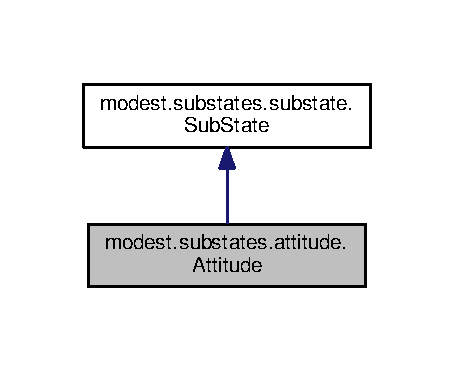
\includegraphics[width=218pt]{classmodest_1_1substates_1_1attitude_1_1Attitude__inherit__graph}
\end{center}
\end{figure}


Collaboration diagram for modest.\+substates.\+attitude.\+Attitude\+:\nopagebreak
\begin{figure}[H]
\begin{center}
\leavevmode
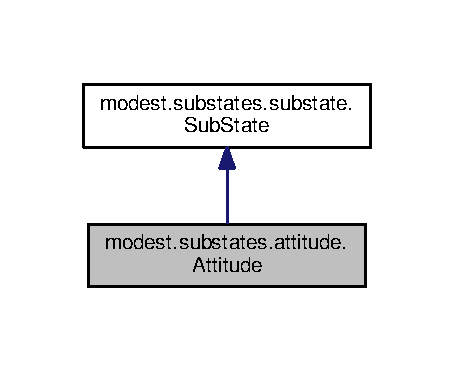
\includegraphics[width=218pt]{classmodest_1_1substates_1_1attitude_1_1Attitude__coll__graph}
\end{center}
\end{figure}
\subsection*{Public Member Functions}
\begin{DoxyCompactItemize}
\item 
def \hyperlink{classmodest_1_1substates_1_1attitude_1_1Attitude_a6ae719302c377bbdb530a2edc4aa9f63}{\+\_\+\+\_\+init\+\_\+\+\_\+} (self, attitude\+Quaternion=Quaternion(\mbox{[}1, 0, 0, 0\mbox{]}), attitude\+Error\+Covariance=np.\+eye(3), gyro\+Bias=np.\+zeros(3), gyro\+Bias\+Covariance=np.\+eye(3), t=0)
\begin{DoxyCompactList}\small\item\em The \hyperlink{classmodest_1_1substates_1_1attitude_1_1Attitude_a6ae719302c377bbdb530a2edc4aa9f63}{\+\_\+\+\_\+init\+\_\+\+\_\+} method initializes the 6\+D\+OF attitude estimator \end{DoxyCompactList}\item 
def \hyperlink{classmodest_1_1substates_1_1attitude_1_1Attitude_a7ed2c772a331dadab761afd11d980c9e}{store\+State\+Vector} (self, sv\+Dict)
\begin{DoxyCompactList}\small\item\em store\+State\+Vector is responsible for taking an updated version of the state vector, and storing it in the class variables. \end{DoxyCompactList}\item 
def \hyperlink{classmodest_1_1substates_1_1attitude_1_1Attitude_a07af5c587e6576e3421197a20880222e}{time\+Update} (self, dT, dynamics=None)
\begin{DoxyCompactList}\small\item\em time\+Update returns the time-\/update matrices, and handles the internal time update of the attitude estimate \hyperlink{classmodest_1_1substates_1_1attitude_1_1Attitude_a22a550534d908153baef2e52f7142c5e}{q\+Hat}. \end{DoxyCompactList}\item 
def \hyperlink{classmodest_1_1substates_1_1attitude_1_1Attitude_ac150d71af97353d06dda45984d20dbab}{get\+Measurement\+Matrices} (self, measurement, source=None)
\begin{DoxyCompactList}\small\item\em get\+Measurement\+Matrices computes and returns measurement update matrices \end{DoxyCompactList}\item 
def \hyperlink{classmodest_1_1substates_1_1attitude_1_1Attitude_ae21ed62061b674b0108f205df2122083}{quaternion\+Time\+Update\+Matrix} (self, my\+Omega, deltaT)
\begin{DoxyCompactList}\small\item\em quaternion\+Time\+Update\+Matrix produces a time-\/update matrix for the attitude quaternion \end{DoxyCompactList}\item 
def \hyperlink{classmodest_1_1substates_1_1attitude_1_1Attitude_a06165c15ac5d7422a7bcd1e3f7ac24e7}{error\+State\+Time\+Update\+Matrix} (self, my\+Omega, deltaT)
\begin{DoxyCompactList}\small\item\em error\+State\+Time\+Update\+Matrix produces a time-\/update matrix for the attitude error state \end{DoxyCompactList}\item 
def \hyperlink{classmodest_1_1substates_1_1attitude_1_1Attitude_a11f6e9a0803c6843d7c89061ffbb3c2c}{process\+Noise\+Matrix} (self, deltaT, omega\+Var, bias\+Var)
\begin{DoxyCompactList}\small\item\em process\+Noise\+Matrix generates a the process noise matrix \end{DoxyCompactList}\item 
def \hyperlink{classmodest_1_1substates_1_1attitude_1_1Attitude_a1506706112528d3d926a77121bac7b1c}{Ra\+Dec\+Meas\+Matrices} (self, source, measurement)
\begin{DoxyCompactList}\small\item\em Ra\+Dec\+Meas\+Matrices generates measurement matrices for a angle measurement of a point source. \end{DoxyCompactList}\item 
def \hyperlink{classmodest_1_1substates_1_1attitude_1_1Attitude_aaca8893538cf2e6118214ea9cef69055}{euler\+Angles} (self)
\begin{DoxyCompactList}\small\item\em euler\+Angles computes the Euler angles (roll, pitch and yaw) based on the current attitude. \end{DoxyCompactList}\item 
def \hyperlink{classmodest_1_1substates_1_1attitude_1_1Attitude_a6fdadf88372f53c3ac216eaf015947db}{Ra\+Dec\+Roll} (self)
\begin{DoxyCompactList}\small\item\em Ra\+Dec\+Roll returns the current attitude in terms of right ascension, declination, and roll \end{DoxyCompactList}\item 
def \hyperlink{classmodest_1_1substates_1_1attitude_1_1Attitude_ae6d69671cf2517be4ad69bee7498e665}{sid\+Unit\+Vec} (self, Ra\+Dec)
\begin{DoxyCompactList}\small\item\em sid\+Unit\+Vec generates a unit vector from two angles \end{DoxyCompactList}\item 
def \hyperlink{classmodest_1_1substates_1_1attitude_1_1Attitude_ae6f156a198d9c2328ddffde498c1ca19}{skew\+Symmetric} (self, vector)
\begin{DoxyCompactList}\small\item\em skew\+Symmetric generates a skew-\/symmetric matrix from a 3x1 vector \end{DoxyCompactList}\end{DoxyCompactItemize}
\begin{Indent}{\bf Mandatory Sub\+State Functions}\par
{\em The following functions are functions which are required for the Sub\+State to function as a sub-\/state in State.\+Modular\+Filter. }\begin{DoxyCompactItemize}
\item 
def \hyperlink{classmodest_1_1substates_1_1substate_1_1SubState_aa18c8238415131b4b63cef0e4b2ff9fd}{get\+State\+Vector} (self)
\begin{DoxyCompactList}\small\item\em \hyperlink{classmodest_1_1substates_1_1substate_1_1SubState_aa18c8238415131b4b63cef0e4b2ff9fd}{get\+State\+Vector} returns the most recent value of the state vector \end{DoxyCompactList}\item 
def \hyperlink{classmodest_1_1substates_1_1substate_1_1SubState_a6e308aadd13962e476d2892ec728e3a5}{covariance} (self)
\begin{DoxyCompactList}\small\item\em \hyperlink{classmodest_1_1substates_1_1substate_1_1SubState_a6e308aadd13962e476d2892ec728e3a5}{covariance} returns the \hyperlink{classmodest_1_1substates_1_1substate_1_1SubState}{Sub\+State} covariance matrix \end{DoxyCompactList}\item 
def \hyperlink{classmodest_1_1substates_1_1substate_1_1SubState_ab9027f6d1d7d57c47731612f519b7ee6}{dimension} (self)
\begin{DoxyCompactList}\small\item\em \hyperlink{classmodest_1_1substates_1_1substate_1_1SubState_ab9027f6d1d7d57c47731612f519b7ee6}{dimension} returns the dimension of the sub-\/state vector \end{DoxyCompactList}\end{DoxyCompactItemize}
\end{Indent}
\begin{Indent}{\bf Plotting Functions}\par
{\em These functions provide generalized plotting capabilities }\begin{DoxyCompactItemize}
\item 
def \hyperlink{classmodest_1_1substates_1_1substate_1_1SubState_a1adac64be88eab0a64bb952518c4268f}{initialize\+Real\+Time\+Plot} (self, plot\+Handle=None, axis\+Handle=None)
\item 
def \hyperlink{classmodest_1_1substates_1_1substate_1_1SubState_a2deb7d1ca3105eb20e50fa7e67298355}{real\+Time\+Plot} (self, normalized=True)
\end{DoxyCompactItemize}
\end{Indent}
\subsection*{Public Attributes}
\begin{DoxyCompactItemize}
\item 
\hyperlink{classmodest_1_1substates_1_1attitude_1_1Attitude_a22a550534d908153baef2e52f7142c5e}{q\+Hat}
\begin{DoxyCompactList}\small\item\em Current estimate of attitude, stored as a Quaternion object Mathematically generally referred to as $\mathbf{\hat{q}}^{-}_{k}$ for the a priori value, or $\mathbf{\hat{q}}^{+}_{k}$ for the a posteriori value. \end{DoxyCompactList}\item 
\hyperlink{classmodest_1_1substates_1_1attitude_1_1Attitude_aac0bc92dc53893d2f190c1252690053c}{b\+Hat}
\begin{DoxyCompactList}\small\item\em Current estimate of gyro bias. \end{DoxyCompactList}\item 
\hyperlink{classmodest_1_1substates_1_1attitude_1_1Attitude_a2f79616ca660e0cc1e628adf94738249}{P\+Hat}
\begin{DoxyCompactList}\small\item\em Current joint covariance matrix. \end{DoxyCompactList}\item 
\hyperlink{classmodest_1_1substates_1_1attitude_1_1Attitude_abc1a273c6fd65c839184ae644b68f010}{last\+Meas\+ID}
\begin{DoxyCompactList}\small\item\em Last measurement used to generate measurement matrices. \end{DoxyCompactList}\item 
\hyperlink{classmodest_1_1substates_1_1attitude_1_1Attitude_a0ec5bf8475ca5c175e4a516d2ac68fdf}{last\+Source\+ID}
\begin{DoxyCompactList}\small\item\em Last signal used to generate measurement matrices. \end{DoxyCompactList}\item 
\hyperlink{classmodest_1_1substates_1_1attitude_1_1Attitude_add344f4323848f4ccdd9e59d699310a0}{last\+Meas\+Mat}
\begin{DoxyCompactList}\small\item\em Last set of measurement matrices. \end{DoxyCompactList}\item 
\hyperlink{classmodest_1_1substates_1_1substate_1_1SubState_a38c12c9d0899bc1161f3502b584517a2}{state\+Vector\+History}
\begin{DoxyCompactList}\small\item\em Stores the time-\/history of the sub-\/state state vector. \end{DoxyCompactList}\item 
\hyperlink{classmodest_1_1substates_1_1substate_1_1SubState_a37ded775b84cea85b4dce0f1b16286c4}{R\+T\+Plot\+Handle}
\begin{DoxyCompactList}\small\item\em Stores handle for real-\/time plotting. \end{DoxyCompactList}\item 
\hyperlink{classmodest_1_1substates_1_1substate_1_1SubState_a9fefae1facc797a1132fb61a55e9ffa1}{R\+T\+Plot\+Data}
\item 
\hyperlink{classmodest_1_1substates_1_1substate_1_1SubState_a497ccbb6658589b02568e87c6382222e}{R\+T\+Paxis\+Handle}
\end{DoxyCompactItemize}


\subsection{Detailed Description}
Estimates the attitude of a vehicle in three dimensions, along with three gyro bias states. 

This class contains a six-\/state attitude estimator\+: three attitude states and three gyro bias states.

This class can function as a stand-\/alone class, or it can function as a \char`\"{}\+Sub\+State\char`\"{} of the State.\+Modular\+Filter class. The functions required for use as a Sub\+State are defined first after {\bfseries init}, then functions specific to this class are defined next.

The state uses quaternions to store attitude, which avoids issues of gimbal lock and increases numerical stability over other approaches, such as Euler angles. The quaternion itself is not treated as a part of the state vector. Rather, the state vector includes three attitude \char`\"{}error states,\char`\"{} which are updated at each measurement, then used to correct the attitude quaternion. After each correction, the error states are set back to zero.

The algorithms used for the state update mostly come from the book \char`\"{}\+Fundamentals of Spacecraft Attitude Determination and Control\char`\"{} (F\+S\+A\+DC) by Markley and Crassidis. Chapter, section and page numbers will be referenced where appropriate. 

Definition at line 38 of file attitude.\+py.



\subsection{Constructor \& Destructor Documentation}
\index{modest\+::substates\+::attitude\+::\+Attitude@{modest\+::substates\+::attitude\+::\+Attitude}!\+\_\+\+\_\+init\+\_\+\+\_\+@{\+\_\+\+\_\+init\+\_\+\+\_\+}}
\index{\+\_\+\+\_\+init\+\_\+\+\_\+@{\+\_\+\+\_\+init\+\_\+\+\_\+}!modest\+::substates\+::attitude\+::\+Attitude@{modest\+::substates\+::attitude\+::\+Attitude}}
\subsubsection[{\texorpdfstring{\+\_\+\+\_\+init\+\_\+\+\_\+(self, attitude\+Quaternion=\+Quaternion([1, 0, 0, 0]), attitude\+Error\+Covariance=np.\+eye(3), gyro\+Bias=np.\+zeros(3), gyro\+Bias\+Covariance=np.\+eye(3), t=0)}{__init__(self, attitudeQuaternion=Quaternion([1, 0, 0, 0]), attitudeErrorCovariance=np.eye(3), gyroBias=np.zeros(3), gyroBiasCovariance=np.eye(3), t=0)}}]{\setlength{\rightskip}{0pt plus 5cm}def modest.\+substates.\+attitude.\+Attitude.\+\_\+\+\_\+init\+\_\+\+\_\+ (
\begin{DoxyParamCaption}
\item[{}]{self, }
\item[{}]{attitude\+Quaternion = {\ttfamily Quaternion(\mbox{[}1,0,0,0\mbox{]})}, }
\item[{}]{attitude\+Error\+Covariance = {\ttfamily np.eye(3)}, }
\item[{}]{gyro\+Bias = {\ttfamily np.zeros(3)}, }
\item[{}]{gyro\+Bias\+Covariance = {\ttfamily np.eye(3)}, }
\item[{}]{t = {\ttfamily 0}}
\end{DoxyParamCaption}
)}\hypertarget{classmodest_1_1substates_1_1attitude_1_1Attitude_a6ae719302c377bbdb530a2edc4aa9f63}{}\label{classmodest_1_1substates_1_1attitude_1_1Attitude_a6ae719302c377bbdb530a2edc4aa9f63}


The \hyperlink{classmodest_1_1substates_1_1attitude_1_1Attitude_a6ae719302c377bbdb530a2edc4aa9f63}{\+\_\+\+\_\+init\+\_\+\+\_\+} method initializes the 6\+D\+OF attitude estimator 

This function is responsible for initializing an instance of the \hyperlink{classmodest_1_1substates_1_1attitude_1_1Attitude}{Attitude} class and storing all the variables as member variables.


\begin{DoxyParams}{Parameters}
{\em self} & The object pointer \\
\hline
{\em attitude\+Quaternion} & A pyquaternion.\+Quaternion object containing the initial attitude estimate. This variable gets stored as \hyperlink{classmodest_1_1substates_1_1attitude_1_1Attitude_a22a550534d908153baef2e52f7142c5e}{q\+Hat}. \\
\hline
{\em attitude\+Error\+Covariance} & A 3x3 numpy array containing the covariance of the current attitude estimate. This matrix is used to form the upper diagonal part of \hyperlink{classmodest_1_1substates_1_1attitude_1_1Attitude_a2f79616ca660e0cc1e628adf94738249}{P\+Hat}. \\
\hline
{\em gyro\+Bias} & A 3 dimensional numpy array containing the estimate of gyro bias. This array is stored as \hyperlink{classmodest_1_1substates_1_1attitude_1_1Attitude_aac0bc92dc53893d2f190c1252690053c}{b\+Hat}. \\
\hline
{\em gyro\+Bias\+Covariance} & A 3x3 numpy array containing the estimate of covariance of gyro bias. This array is used to form the lower diagonal part of \hyperlink{classmodest_1_1substates_1_1attitude_1_1Attitude_a2f79616ca660e0cc1e628adf94738249}{P\+Hat}. \\
\hline
\end{DoxyParams}


Definition at line 64 of file attitude.\+py.



\subsection{Member Function Documentation}
\index{modest\+::substates\+::attitude\+::\+Attitude@{modest\+::substates\+::attitude\+::\+Attitude}!covariance@{covariance}}
\index{covariance@{covariance}!modest\+::substates\+::attitude\+::\+Attitude@{modest\+::substates\+::attitude\+::\+Attitude}}
\subsubsection[{\texorpdfstring{covariance(self)}{covariance(self)}}]{\setlength{\rightskip}{0pt plus 5cm}def modest.\+substates.\+substate.\+Sub\+State.\+covariance (
\begin{DoxyParamCaption}
\item[{}]{self}
\end{DoxyParamCaption}
)\hspace{0.3cm}{\ttfamily [inherited]}}\hypertarget{classmodest_1_1substates_1_1substate_1_1SubState_a6e308aadd13962e476d2892ec728e3a5}{}\label{classmodest_1_1substates_1_1substate_1_1SubState_a6e308aadd13962e476d2892ec728e3a5}


\hyperlink{classmodest_1_1substates_1_1substate_1_1SubState_a6e308aadd13962e476d2892ec728e3a5}{covariance} returns the \hyperlink{classmodest_1_1substates_1_1substate_1_1SubState}{Sub\+State} covariance matrix 

The \hyperlink{classmodest_1_1substates_1_1substate_1_1SubState_a6e308aadd13962e476d2892ec728e3a5}{covariance} method returns the covariance of the estimate of the substate.

\begin{DoxyRefDesc}{Todo}
\item[\hyperlink{todo__todo000001}{Todo}]Currently, this method only returns the covariance of the most recent state estimate. Ideally, there should be an optional time parameter which would allow the user to get the covaraince matrix at a specified time (or the closest to that specified time).\end{DoxyRefDesc}



\begin{DoxyParams}{Parameters}
{\em self} & The object pointer\\
\hline
\end{DoxyParams}
\begin{DoxyReturn}{Returns}
Returns the covaraince matrix 
\end{DoxyReturn}


Definition at line 172 of file substate.\+py.

\index{modest\+::substates\+::attitude\+::\+Attitude@{modest\+::substates\+::attitude\+::\+Attitude}!dimension@{dimension}}
\index{dimension@{dimension}!modest\+::substates\+::attitude\+::\+Attitude@{modest\+::substates\+::attitude\+::\+Attitude}}
\subsubsection[{\texorpdfstring{dimension(self)}{dimension(self)}}]{\setlength{\rightskip}{0pt plus 5cm}def modest.\+substates.\+substate.\+Sub\+State.\+dimension (
\begin{DoxyParamCaption}
\item[{}]{self}
\end{DoxyParamCaption}
)\hspace{0.3cm}{\ttfamily [inherited]}}\hypertarget{classmodest_1_1substates_1_1substate_1_1SubState_ab9027f6d1d7d57c47731612f519b7ee6}{}\label{classmodest_1_1substates_1_1substate_1_1SubState_ab9027f6d1d7d57c47731612f519b7ee6}


\hyperlink{classmodest_1_1substates_1_1substate_1_1SubState_ab9027f6d1d7d57c47731612f519b7ee6}{dimension} returns the dimension of the sub-\/state vector 

The \hyperlink{classmodest_1_1substates_1_1substate_1_1SubState_ab9027f6d1d7d57c47731612f519b7ee6}{dimension} method returns the dimension of the sub-\/state vector estimated by the \hyperlink{classmodest_1_1substates_1_1substate_1_1SubState}{Sub\+State}. This is the dimension as seen by the \hyperlink{namespacemodest_1_1ModularFilter}{Modular\+Filter} estimator.

The default implementation is to return the class variable \hyperlink{classmodest_1_1substates_1_1substate_1_1SubState_a5b1c0756a69da7f293a415c7d2d77843}{\+\_\+\+\_\+dimension\+\_\+\+\_\+}, which is saved at initialization. This is designated as a \char`\"{}protected\char`\"{} variable, and should not change during the course of the \hyperlink{classmodest_1_1substates_1_1substate_1_1SubState}{Sub\+State}\textquotesingle{}s lifetime. If child class overwrites this implementation, care should be taken to ensure that the value returned by \hyperlink{classmodest_1_1substates_1_1substate_1_1SubState_ab9027f6d1d7d57c47731612f519b7ee6}{dimension} does not change over \hyperlink{classmodest_1_1substates_1_1substate_1_1SubState}{Sub\+State} object lifetime.

For \hyperlink{classmodest_1_1substates_1_1substate_1_1SubState}{Sub\+State} objects with auxilary states, or other quantities related to the state vector but not directly estimated by the \hyperlink{namespacemodest_1_1ModularFilter}{Modular\+Filter}, \hyperlink{classmodest_1_1substates_1_1substate_1_1SubState_ab9027f6d1d7d57c47731612f519b7ee6}{dimension} should not count these states as part of the total dimension.


\begin{DoxyParams}{Parameters}
{\em self} & The object pointer\\
\hline
\end{DoxyParams}
\begin{DoxyReturn}{Returns}
Returns the dimension of state vector 
\end{DoxyReturn}


Definition at line 197 of file substate.\+py.

\index{modest\+::substates\+::attitude\+::\+Attitude@{modest\+::substates\+::attitude\+::\+Attitude}!error\+State\+Time\+Update\+Matrix@{error\+State\+Time\+Update\+Matrix}}
\index{error\+State\+Time\+Update\+Matrix@{error\+State\+Time\+Update\+Matrix}!modest\+::substates\+::attitude\+::\+Attitude@{modest\+::substates\+::attitude\+::\+Attitude}}
\subsubsection[{\texorpdfstring{error\+State\+Time\+Update\+Matrix(self, my\+Omega, delta\+T)}{errorStateTimeUpdateMatrix(self, myOmega, deltaT)}}]{\setlength{\rightskip}{0pt plus 5cm}def modest.\+substates.\+attitude.\+Attitude.\+error\+State\+Time\+Update\+Matrix (
\begin{DoxyParamCaption}
\item[{}]{self, }
\item[{}]{my\+Omega, }
\item[{}]{deltaT}
\end{DoxyParamCaption}
)}\hypertarget{classmodest_1_1substates_1_1attitude_1_1Attitude_a06165c15ac5d7422a7bcd1e3f7ac24e7}{}\label{classmodest_1_1substates_1_1attitude_1_1Attitude_a06165c15ac5d7422a7bcd1e3f7ac24e7}


error\+State\+Time\+Update\+Matrix produces a time-\/update matrix for the attitude error state 

This function the discrete-\/time error-\/state transition matrix. This is the matrix which propagates the attitude error state covariance and gyro bias covariance forward in time based on time ellapsed and angular velocity estimate.

The error-\/state transition matrix is defined as follows\+:

\[ \boldsymbol{\Phi} = \begin{bmatrix} \boldsymbol{\Phi}_{11} & \boldsymbol{\Phi}_{12} \\ \boldsymbol{\Phi}_{21} & \boldsymbol{\Phi}_{22} \\ \end{bmatrix} \]

where

\[ \boldsymbol{\Phi}_{11} = \eye[3] - \left[\omegaVec[est=True,aPriori=True, t=k] \times \right] \frac {\textrm{sin}(||\omegaVec[est=True,aPriori=True, t=k]|| \Delta t)} {||\omegaVec[est=True,aPriori=True, t=k]||} + \left[\omegaVec[est=True,aPriori=True, t=k] \times \right]^2 \frac {1 - \textrm{cos}(1 - ||\omegaVec[est=True,aPriori=True, t=k]|| \Delta t)} {||\omegaVec[est=True,aPriori=True, t=k]||^2} \]

\[ \boldsymbol{\Phi}_{12} = \left[\omegaVec[est=True,aPriori=True, t=k] \times \right] \frac {1 - \textrm{cos}(1 - ||\omegaVec[est=True,aPriori=True, t=k]|| \Delta t)} {||\omegaVec[est=True,aPriori=True, t=k]||^2} - \eye[3]\Delta t - \left[\omegaVec[est=True,aPriori=True, t=k] \times \right]^2 \frac {||\omegaVec[est=True,aPriori=True, t=k]|| \Delta t - \textrm{sin}(||\omegaVec[est=True,aPriori=True, t=k]|| \Delta t)} {||\omegaVec[est=True,aPriori=True, t=k]||^3} \]

\[ \boldsymbol{\Phi}_{21} = \mathbf{0}_{3 \times 3} \]

\[ \boldsymbol{\Phi}_{22} = \eye[3] \]

See Fundamentals of Spacecraft \hyperlink{classmodest_1_1substates_1_1attitude_1_1Attitude}{Attitude} Determination and Control, Section 6.\+2.\+4, page 258, equation 6.\+83 for more details and derivation.


\begin{DoxyParams}{Parameters}
{\em self} & The object pointer \\
\hline
{\em my\+Omega} & The angular velocity estimate used to update the attitude quaternion \\
\hline
{\em deltaT} & The amount of time elapsed for the time-\/update, used for numerical integration of kinematics equation.\\
\hline
\end{DoxyParams}
\begin{DoxyReturn}{Returns}
Returns the error-\/state time update matrix, $\boldsymbol{\Phi}$ 
\end{DoxyReturn}


Definition at line 464 of file attitude.\+py.

\index{modest\+::substates\+::attitude\+::\+Attitude@{modest\+::substates\+::attitude\+::\+Attitude}!euler\+Angles@{euler\+Angles}}
\index{euler\+Angles@{euler\+Angles}!modest\+::substates\+::attitude\+::\+Attitude@{modest\+::substates\+::attitude\+::\+Attitude}}
\subsubsection[{\texorpdfstring{euler\+Angles(self)}{eulerAngles(self)}}]{\setlength{\rightskip}{0pt plus 5cm}def modest.\+substates.\+attitude.\+Attitude.\+euler\+Angles (
\begin{DoxyParamCaption}
\item[{}]{self}
\end{DoxyParamCaption}
)}\hypertarget{classmodest_1_1substates_1_1attitude_1_1Attitude_aaca8893538cf2e6118214ea9cef69055}{}\label{classmodest_1_1substates_1_1attitude_1_1Attitude_aaca8893538cf2e6118214ea9cef69055}


euler\+Angles computes the Euler angles (roll, pitch and yaw) based on the current attitude. 

This function computes the Euler angles (or, technically the \char`\"{}\+Tait-\/\+Bryan angles\char`\"{}), i.\+e. roll, pitch and yaw from the current attitude quaternion \hyperlink{classmodest_1_1substates_1_1attitude_1_1Attitude_a22a550534d908153baef2e52f7142c5e}{q\+Hat}.

\begin{DoxyNote}{Note}
See Wikipedia\textquotesingle{}s article on the \href{https://en.wikipedia.org/wiki/Euler_angles}{\tt equatorial coordinate system} for more details.
\end{DoxyNote}

\begin{DoxyParams}{Parameters}
{\em self} & The object pointer\\
\hline
\end{DoxyParams}
\begin{DoxyReturn}{Returns}
A list containing the three angles 
\end{DoxyReturn}


Definition at line 695 of file attitude.\+py.

\index{modest\+::substates\+::attitude\+::\+Attitude@{modest\+::substates\+::attitude\+::\+Attitude}!get\+Measurement\+Matrices@{get\+Measurement\+Matrices}}
\index{get\+Measurement\+Matrices@{get\+Measurement\+Matrices}!modest\+::substates\+::attitude\+::\+Attitude@{modest\+::substates\+::attitude\+::\+Attitude}}
\subsubsection[{\texorpdfstring{get\+Measurement\+Matrices(self, measurement, source=\+None)}{getMeasurementMatrices(self, measurement, source=None)}}]{\setlength{\rightskip}{0pt plus 5cm}def modest.\+substates.\+attitude.\+Attitude.\+get\+Measurement\+Matrices (
\begin{DoxyParamCaption}
\item[{}]{self, }
\item[{}]{measurement, }
\item[{}]{source = {\ttfamily None}}
\end{DoxyParamCaption}
)}\hypertarget{classmodest_1_1substates_1_1attitude_1_1Attitude_ac150d71af97353d06dda45984d20dbab}{}\label{classmodest_1_1substates_1_1attitude_1_1Attitude_ac150d71af97353d06dda45984d20dbab}


get\+Measurement\+Matrices computes and returns measurement update matrices 

This function receives a dictionary containing a measurement, along with an object that contains the source model of the measurement. If the source is a Signals.\+Point\+Source type signal, then it generates unit-\/vector attitude measurement type matrices. Otherwise, the function returns dicts populated with None.

\begin{DoxyNote}{Note}
This function is one of mandatory functions required for AttitudeS to function as a sub-\/state of State.\+Modular\+Filter.
\end{DoxyNote}

\begin{DoxyParams}{Parameters}
{\em self} & The object pointer \\
\hline
{\em measurement} & A dictionary containing measurement information \\
\hline
{\em source} & The source object that produced the measurement\\
\hline
\end{DoxyParams}
\begin{DoxyReturn}{Returns}
A dictionary containing the measurement matrices H, R, and dY
\end{DoxyReturn}
\begin{DoxySeeAlso}{See also}
Sub\+States.\+Sub\+State.\+get\+Measurement\+Matrices 
\end{DoxySeeAlso}


Definition at line 285 of file attitude.\+py.

\index{modest\+::substates\+::attitude\+::\+Attitude@{modest\+::substates\+::attitude\+::\+Attitude}!get\+State\+Vector@{get\+State\+Vector}}
\index{get\+State\+Vector@{get\+State\+Vector}!modest\+::substates\+::attitude\+::\+Attitude@{modest\+::substates\+::attitude\+::\+Attitude}}
\subsubsection[{\texorpdfstring{get\+State\+Vector(self)}{getStateVector(self)}}]{\setlength{\rightskip}{0pt plus 5cm}def modest.\+substates.\+substate.\+Sub\+State.\+get\+State\+Vector (
\begin{DoxyParamCaption}
\item[{}]{self}
\end{DoxyParamCaption}
)\hspace{0.3cm}{\ttfamily [inherited]}}\hypertarget{classmodest_1_1substates_1_1substate_1_1SubState_aa18c8238415131b4b63cef0e4b2ff9fd}{}\label{classmodest_1_1substates_1_1substate_1_1SubState_aa18c8238415131b4b63cef0e4b2ff9fd}


\hyperlink{classmodest_1_1substates_1_1substate_1_1SubState_aa18c8238415131b4b63cef0e4b2ff9fd}{get\+State\+Vector} returns the most recent value of the state vector 

The \hyperlink{classmodest_1_1substates_1_1substate_1_1SubState_aa18c8238415131b4b63cef0e4b2ff9fd}{get\+State\+Vector} method is responsible for returning a dictionary object containing, at minimim, the following items\+:


\begin{DoxyItemize}
\item \textquotesingle{}state\+Vector\textquotesingle{}\+: A length \hyperlink{classmodest_1_1substates_1_1substate_1_1SubState_ab9027f6d1d7d57c47731612f519b7ee6}{dimension} array containing the most recent state vector estimate
\item \textquotesingle{}covariance\textquotesingle{}\+: A (\hyperlink{classmodest_1_1substates_1_1substate_1_1SubState_ab9027f6d1d7d57c47731612f519b7ee6}{dimension} x \hyperlink{classmodest_1_1substates_1_1substate_1_1SubState_ab9027f6d1d7d57c47731612f519b7ee6}{dimension}) array containing the most recent covariance matrix
\item \textquotesingle{}a\+Priori\textquotesingle{}\+: A boolean indicating if the most recent estimate is the
\item result of a time update (a\+Priori=True) or a measurement update (a\+Priori=False)
\end{DoxyItemize}

This function can be used as-\/is


\begin{DoxyParams}{Parameters}
{\em self} & The object pointer\\
\hline
\end{DoxyParams}
\begin{DoxyReturn}{Returns}
The dictionary containing the state vector, covariance matrix, and a\+Priori status 
\end{DoxyReturn}


Definition at line 129 of file substate.\+py.

\index{modest\+::substates\+::attitude\+::\+Attitude@{modest\+::substates\+::attitude\+::\+Attitude}!initialize\+Real\+Time\+Plot@{initialize\+Real\+Time\+Plot}}
\index{initialize\+Real\+Time\+Plot@{initialize\+Real\+Time\+Plot}!modest\+::substates\+::attitude\+::\+Attitude@{modest\+::substates\+::attitude\+::\+Attitude}}
\subsubsection[{\texorpdfstring{initialize\+Real\+Time\+Plot(self, plot\+Handle=\+None, axis\+Handle=\+None)}{initializeRealTimePlot(self, plotHandle=None, axisHandle=None)}}]{\setlength{\rightskip}{0pt plus 5cm}def modest.\+substates.\+substate.\+Sub\+State.\+initialize\+Real\+Time\+Plot (
\begin{DoxyParamCaption}
\item[{}]{self, }
\item[{}]{plot\+Handle = {\ttfamily None}, }
\item[{}]{axis\+Handle = {\ttfamily None}}
\end{DoxyParamCaption}
)\hspace{0.3cm}{\ttfamily [inherited]}}\hypertarget{classmodest_1_1substates_1_1substate_1_1SubState_a1adac64be88eab0a64bb952518c4268f}{}\label{classmodest_1_1substates_1_1substate_1_1SubState_a1adac64be88eab0a64bb952518c4268f}


Definition at line 257 of file substate.\+py.

\index{modest\+::substates\+::attitude\+::\+Attitude@{modest\+::substates\+::attitude\+::\+Attitude}!process\+Noise\+Matrix@{process\+Noise\+Matrix}}
\index{process\+Noise\+Matrix@{process\+Noise\+Matrix}!modest\+::substates\+::attitude\+::\+Attitude@{modest\+::substates\+::attitude\+::\+Attitude}}
\subsubsection[{\texorpdfstring{process\+Noise\+Matrix(self, delta\+T, omega\+Var, bias\+Var)}{processNoiseMatrix(self, deltaT, omegaVar, biasVar)}}]{\setlength{\rightskip}{0pt plus 5cm}def modest.\+substates.\+attitude.\+Attitude.\+process\+Noise\+Matrix (
\begin{DoxyParamCaption}
\item[{}]{self, }
\item[{}]{deltaT, }
\item[{}]{omega\+Var, }
\item[{}]{bias\+Var}
\end{DoxyParamCaption}
)}\hypertarget{classmodest_1_1substates_1_1attitude_1_1Attitude_a11f6e9a0803c6843d7c89061ffbb3c2c}{}\label{classmodest_1_1substates_1_1attitude_1_1Attitude_a11f6e9a0803c6843d7c89061ffbb3c2c}


process\+Noise\+Matrix generates a the process noise matrix 

This function generates the process noise matrix for time update of attitude error covariance and gyro bias covariance. The process noise matrix is a function propagation time, angular velocity noise, and gyro bias noise. It is defined as follows\+:

\[ \mathbf{Q} = \begin{bmatrix} \left(\sigma_v^2 \Delta t + \frac{1}{3}\sigma_u^2 \Delta t^3\right) \eye[3] & -\left( \frac{1}{2} \sigma_u^2 \Delta t^2 \right) \eye[3] \\ -\left( \frac{1}{2} \sigma_u^2 \Delta t^2 \right) \eye[3] & \left( \sigma_u^2 \Delta t \right) \eye[3] \end{bmatrix} \]

where $\sigma_v^2$ is the angular velocity noise (i.\+e. gyro measurement noise) and $ \sigma_u^2 $ is the gyro bias process noise.

See Fundamentals of Spacecraft \hyperlink{classmodest_1_1substates_1_1attitude_1_1Attitude}{Attitude} Determination and Control, Section 6.\+2.\+4, page 260, equation 6.\+93 for derivation and more details.


\begin{DoxyParams}{Parameters}
{\em self} & The object pointer \\
\hline
{\em deltaT} & The amount of time corresponding to the time update \\
\hline
{\em omega\+Var} & The variance of the angular velocity (gyro) measurement \\
\hline
{\em bias\+Var} & The variance of the gias bias process noise (indicates how much the gyro bias changes over time) \\
\hline
\end{DoxyParams}
\begin{DoxyReturn}{Returns}
Returns the comibined 6x6 process noise matrix 
\end{DoxyReturn}


Definition at line 534 of file attitude.\+py.

\index{modest\+::substates\+::attitude\+::\+Attitude@{modest\+::substates\+::attitude\+::\+Attitude}!quaternion\+Time\+Update\+Matrix@{quaternion\+Time\+Update\+Matrix}}
\index{quaternion\+Time\+Update\+Matrix@{quaternion\+Time\+Update\+Matrix}!modest\+::substates\+::attitude\+::\+Attitude@{modest\+::substates\+::attitude\+::\+Attitude}}
\subsubsection[{\texorpdfstring{quaternion\+Time\+Update\+Matrix(self, my\+Omega, delta\+T)}{quaternionTimeUpdateMatrix(self, myOmega, deltaT)}}]{\setlength{\rightskip}{0pt plus 5cm}def modest.\+substates.\+attitude.\+Attitude.\+quaternion\+Time\+Update\+Matrix (
\begin{DoxyParamCaption}
\item[{}]{self, }
\item[{}]{my\+Omega, }
\item[{}]{deltaT}
\end{DoxyParamCaption}
)}\hypertarget{classmodest_1_1substates_1_1attitude_1_1Attitude_ae21ed62061b674b0108f205df2122083}{}\label{classmodest_1_1substates_1_1attitude_1_1Attitude_ae21ed62061b674b0108f205df2122083}


quaternion\+Time\+Update\+Matrix produces a time-\/update matrix for the attitude quaternion 

This function produces a 4x4 matrix which, when multiplied by an attitude quaternion, rotates the quaternion by an amount corresponding to the angular velocity and time ellapsed. The attitude quaternion is updated as follows\+:

\[ \attVec[est=True,aPriori=True, t=k+1] \approx \bar{\Theta}(\omegaVec[est=True,aPriori=True, t=k], \Delta T) \attVec[est=True, aPriori=False, t=k] \]

where

\[ \bar{\Theta}( \omegaVec[est=True,aPriori=True, t=k], \Delta T ) = \begin{bmatrix} \textrm{cos} \left(\frac{1}{2} ||\omegaVec[est=True,aPriori=True, t=k]|| \Delta t \right) I_3 - \left[\boldsymbol{\hat{\Psi}}_k^+ \times \right] & \left[\boldsymbol{\hat{\Psi}}_k^+ \times \right] \\ - \left[\boldsymbol{\hat{\Psi}}_k^+ \times \right] & \textrm{cos} \left(\frac{1}{2} ||\mathbf{\hat{\omega}}_k^+|| \Delta t \right) \end{bmatrix} \]

and

\[ \left[\boldsymbol{\hat{\Psi}}_k^+ \times \right] = \frac{ \textrm{sin}\left(\frac{1}{2} || \omegaVec[est=True,aPriori=True, t=k] || \Delta t \right) \omegaVec[est=True,aPriori=True, t=k] }{ || \omegaVec[est=True,aPriori=True, t=k] || } \]

The matrix returned by this function is $\bar{\Theta}(\omegaVec[est=True,aPriori=True, t=k], \Delta T)$.

See Fundamentals of Spacecraft \hyperlink{classmodest_1_1substates_1_1attitude_1_1Attitude}{Attitude} Determination and Control, Section 6.\+2.\+2, page 251, equation 6.\+60 for more details.


\begin{DoxyParams}{Parameters}
{\em self} & The object pointer \\
\hline
{\em my\+Omega} & The angular velocity estimate used to update the attitude quaternion \\
\hline
{\em deltaT} & The amount of time elapsed for the time-\/update, used for numerical integration of kinematics equation.\\
\hline
\end{DoxyParams}
\begin{DoxyReturn}{Returns}
The quaternion time-\/update matrix $\bar{\Theta}(\omegaVec[est=True,aPriori=True, t=k], \Delta T)$ 
\end{DoxyReturn}


Definition at line 380 of file attitude.\+py.

\index{modest\+::substates\+::attitude\+::\+Attitude@{modest\+::substates\+::attitude\+::\+Attitude}!Ra\+Dec\+Meas\+Matrices@{Ra\+Dec\+Meas\+Matrices}}
\index{Ra\+Dec\+Meas\+Matrices@{Ra\+Dec\+Meas\+Matrices}!modest\+::substates\+::attitude\+::\+Attitude@{modest\+::substates\+::attitude\+::\+Attitude}}
\subsubsection[{\texorpdfstring{Ra\+Dec\+Meas\+Matrices(self, source, measurement)}{RaDecMeasMatrices(self, source, measurement)}}]{\setlength{\rightskip}{0pt plus 5cm}def modest.\+substates.\+attitude.\+Attitude.\+Ra\+Dec\+Meas\+Matrices (
\begin{DoxyParamCaption}
\item[{}]{self, }
\item[{}]{source, }
\item[{}]{measurement}
\end{DoxyParamCaption}
)}\hypertarget{classmodest_1_1substates_1_1attitude_1_1Attitude_a1506706112528d3d926a77121bac7b1c}{}\label{classmodest_1_1substates_1_1attitude_1_1Attitude_a1506706112528d3d926a77121bac7b1c}


Ra\+Dec\+Meas\+Matrices generates measurement matrices for a angle measurement of a point source. 

This function generates the set of measurement matrices $ \mathbf{H} $, $ \mathbf{dY} $, and $ \mathbf{R} $ corresponding to an inferred unit vector measurement from a set of two angle measurments (local right ascension and declination of a point source).

The measurement matrices are a function of the measurement itself, the source from which the measurement originated, and the current estimate of attitude, \hyperlink{classmodest_1_1substates_1_1attitude_1_1Attitude_a22a550534d908153baef2e52f7142c5e}{q\+Hat}. They are defined as follows\+:

\[ \mathbf{H}_k[\sv[aPriori=True,timeIndex=k]] = A(\attVec[est=True,aPriori=True,t=k]) \unitVec[signalSource=S, frame=nav] \times \]

\[ \mathbf{dY} = \measurementVec[S](\RADEC) - A(\attVec[est=True,aPriori=True,t=k]) \unitVec[signalSource=S, frame=nav] \]

\[ \mathbf{R} = \eye[3] \sigma^2_{\RADEC} \]

The measured unit vector is a unit vector computed from the measured angles, using \hyperlink{classmodest_1_1substates_1_1attitude_1_1Attitude_ae6d69671cf2517be4ad69bee7498e665}{sid\+Unit\+Vec}.

See Fundamentals of Spacecraft \hyperlink{classmodest_1_1substates_1_1attitude_1_1Attitude}{Attitude} Determination and Control, Section 6.\+2.\+4, page 257, Table 6.\+3 for more details and derivation.

\begin{DoxyNote}{Note}
Currently, the measurement noise matrix is an identity matrix mutiplied by the angle measurement error. This is my interpretation of Section 6.\+2.\+3 in F\+S\+A\+DC. However, if we derive the measurement noise matrix using the usual E\+KF method, we get a different result which results in an unstable estimator. I\textquotesingle{}m not convinced I understand why this method is right, or why the E\+KF method is unstable, but it works, so we\textquotesingle{}re using it for now.
\end{DoxyNote}

\begin{DoxyParams}{Parameters}
{\em self} & The object pointer \\
\hline
{\em source} & A Signals.\+Point\+Source object from which the measurement was generated. \\
\hline
{\em measurement} & A dictionary containing the right ascension and declination measurements as sub-\/dictionaries, each with their own value and variance.\\
\hline
\end{DoxyParams}
\begin{DoxyReturn}{Returns}
A dictionary containing the measurement matrices H, R, and dY 
\end{DoxyReturn}


Definition at line 613 of file attitude.\+py.

\index{modest\+::substates\+::attitude\+::\+Attitude@{modest\+::substates\+::attitude\+::\+Attitude}!Ra\+Dec\+Roll@{Ra\+Dec\+Roll}}
\index{Ra\+Dec\+Roll@{Ra\+Dec\+Roll}!modest\+::substates\+::attitude\+::\+Attitude@{modest\+::substates\+::attitude\+::\+Attitude}}
\subsubsection[{\texorpdfstring{Ra\+Dec\+Roll(self)}{RaDecRoll(self)}}]{\setlength{\rightskip}{0pt plus 5cm}def modest.\+substates.\+attitude.\+Attitude.\+Ra\+Dec\+Roll (
\begin{DoxyParamCaption}
\item[{}]{self}
\end{DoxyParamCaption}
)}\hypertarget{classmodest_1_1substates_1_1attitude_1_1Attitude_a6fdadf88372f53c3ac216eaf015947db}{}\label{classmodest_1_1substates_1_1attitude_1_1Attitude_a6fdadf88372f53c3ac216eaf015947db}


Ra\+Dec\+Roll returns the current attitude in terms of right ascension, declination, and roll 

This function essentially computes the euler angles (1-\/2-\/3) from the current attitude quaternion \hyperlink{classmodest_1_1substates_1_1attitude_1_1Attitude_a22a550534d908153baef2e52f7142c5e}{q\+Hat} and returns them in reverse order (3-\/2-\/1). This is helpful because the attitude of spacecraft is commonly expressed in terms of R\+A-\/\+Dec-\/\+Roll, rather than roll-\/pitch-\/yaw which is more standard in other aerospace applications.

\begin{DoxyNote}{Note}
See Wikipedia\textquotesingle{}s article on the \href{https://en.wikipedia.org/wiki/Equatorial_coordinate_system}{\tt equatorial coordinate system} for more details.
\end{DoxyNote}

\begin{DoxyParams}{Parameters}
{\em self} & The object pointer\\
\hline
\end{DoxyParams}
\begin{DoxyReturn}{Returns}
A list containing the three angles 
\end{DoxyReturn}


Definition at line 719 of file attitude.\+py.

\index{modest\+::substates\+::attitude\+::\+Attitude@{modest\+::substates\+::attitude\+::\+Attitude}!real\+Time\+Plot@{real\+Time\+Plot}}
\index{real\+Time\+Plot@{real\+Time\+Plot}!modest\+::substates\+::attitude\+::\+Attitude@{modest\+::substates\+::attitude\+::\+Attitude}}
\subsubsection[{\texorpdfstring{real\+Time\+Plot(self, normalized=\+True)}{realTimePlot(self, normalized=True)}}]{\setlength{\rightskip}{0pt plus 5cm}def modest.\+substates.\+substate.\+Sub\+State.\+real\+Time\+Plot (
\begin{DoxyParamCaption}
\item[{}]{self, }
\item[{}]{normalized = {\ttfamily True}}
\end{DoxyParamCaption}
)\hspace{0.3cm}{\ttfamily [inherited]}}\hypertarget{classmodest_1_1substates_1_1substate_1_1SubState_a2deb7d1ca3105eb20e50fa7e67298355}{}\label{classmodest_1_1substates_1_1substate_1_1SubState_a2deb7d1ca3105eb20e50fa7e67298355}


Definition at line 283 of file substate.\+py.

\index{modest\+::substates\+::attitude\+::\+Attitude@{modest\+::substates\+::attitude\+::\+Attitude}!sid\+Unit\+Vec@{sid\+Unit\+Vec}}
\index{sid\+Unit\+Vec@{sid\+Unit\+Vec}!modest\+::substates\+::attitude\+::\+Attitude@{modest\+::substates\+::attitude\+::\+Attitude}}
\subsubsection[{\texorpdfstring{sid\+Unit\+Vec(self, Ra\+Dec)}{sidUnitVec(self, RaDec)}}]{\setlength{\rightskip}{0pt plus 5cm}def modest.\+substates.\+attitude.\+Attitude.\+sid\+Unit\+Vec (
\begin{DoxyParamCaption}
\item[{}]{self, }
\item[{}]{Ra\+Dec}
\end{DoxyParamCaption}
)}\hypertarget{classmodest_1_1substates_1_1attitude_1_1Attitude_ae6d69671cf2517be4ad69bee7498e665}{}\label{classmodest_1_1substates_1_1attitude_1_1Attitude_ae6d69671cf2517be4ad69bee7498e665}


sid\+Unit\+Vec generates a unit vector from two angles 

This function computes the unit vector in siderial coordinates from a measurement of right ascension and declination. This is a \char`\"{}helper\char`\"{} function; it doesn\textquotesingle{}t really need to be included in the class and could be moved to a seperate library probably.


\begin{DoxyParams}{Parameters}
{\em self} & Object pointer \\
\hline
{\em Ra\+Dec} & A dictionary containing the two angles\\
\hline
\end{DoxyParams}
\begin{DoxyReturn}{Returns}
A unit vector generated from the angles given 
\end{DoxyReturn}


Definition at line 738 of file attitude.\+py.

\index{modest\+::substates\+::attitude\+::\+Attitude@{modest\+::substates\+::attitude\+::\+Attitude}!skew\+Symmetric@{skew\+Symmetric}}
\index{skew\+Symmetric@{skew\+Symmetric}!modest\+::substates\+::attitude\+::\+Attitude@{modest\+::substates\+::attitude\+::\+Attitude}}
\subsubsection[{\texorpdfstring{skew\+Symmetric(self, vector)}{skewSymmetric(self, vector)}}]{\setlength{\rightskip}{0pt plus 5cm}def modest.\+substates.\+attitude.\+Attitude.\+skew\+Symmetric (
\begin{DoxyParamCaption}
\item[{}]{self, }
\item[{}]{vector}
\end{DoxyParamCaption}
)}\hypertarget{classmodest_1_1substates_1_1attitude_1_1Attitude_ae6f156a198d9c2328ddffde498c1ca19}{}\label{classmodest_1_1substates_1_1attitude_1_1Attitude_ae6f156a198d9c2328ddffde498c1ca19}


skew\+Symmetric generates a skew-\/symmetric matrix from a 3x1 vector 

This function generates a skew symmetric matrix from a 3x1 vector. It is a \char`\"{}helper\char`\"{} function and doesn\textquotesingle{}t actually need to be a member function. It could (should?) be moved to its own library.


\begin{DoxyParams}{Parameters}
{\em self} & Object pointer \\
\hline
{\em vector} & The vector\\
\hline
\end{DoxyParams}
\begin{DoxyReturn}{Returns}
The skew symmetric matrix 
\end{DoxyReturn}


Definition at line 760 of file attitude.\+py.

\index{modest\+::substates\+::attitude\+::\+Attitude@{modest\+::substates\+::attitude\+::\+Attitude}!store\+State\+Vector@{store\+State\+Vector}}
\index{store\+State\+Vector@{store\+State\+Vector}!modest\+::substates\+::attitude\+::\+Attitude@{modest\+::substates\+::attitude\+::\+Attitude}}
\subsubsection[{\texorpdfstring{store\+State\+Vector(self, sv\+Dict)}{storeStateVector(self, svDict)}}]{\setlength{\rightskip}{0pt plus 5cm}def modest.\+substates.\+attitude.\+Attitude.\+store\+State\+Vector (
\begin{DoxyParamCaption}
\item[{}]{self, }
\item[{}]{sv\+Dict}
\end{DoxyParamCaption}
)}\hypertarget{classmodest_1_1substates_1_1attitude_1_1Attitude_a7ed2c772a331dadab761afd11d980c9e}{}\label{classmodest_1_1substates_1_1attitude_1_1Attitude_a7ed2c772a331dadab761afd11d980c9e}


store\+State\+Vector is responsible for taking an updated version of the state vector, and storing it in the class variables. 

This function is designed to receive a time or measurement updated state vector and covariance, and store it. This function is used by State.\+Modular\+Filter to store a jointly updated state.

Depending on whether the state vector is the result of a time update (a\+Priori=True) or a measurement update (a\+Priori=False), the function may disregard the value of the attitude error state. This is because this class handles the time-\/update of \hyperlink{classmodest_1_1substates_1_1attitude_1_1Attitude_a22a550534d908153baef2e52f7142c5e}{q\+Hat} internally, so the updated attitude error state is only relevant after a measurement update.


\begin{DoxyParams}{Parameters}
{\em self} & The object pointer \\
\hline
{\em sv\+Dict} & A dictionary containing the current state vector information. state vector is \char`\"{}a priori\char`\"{} or \char`\"{}a posteriori.\char`\"{}\\
\hline
\end{DoxyParams}
\begin{DoxySeeAlso}{See also}
Sub\+States.\+Sub\+State.\+store\+State\+Vector 
\end{DoxySeeAlso}


Definition at line 146 of file attitude.\+py.

\index{modest\+::substates\+::attitude\+::\+Attitude@{modest\+::substates\+::attitude\+::\+Attitude}!time\+Update@{time\+Update}}
\index{time\+Update@{time\+Update}!modest\+::substates\+::attitude\+::\+Attitude@{modest\+::substates\+::attitude\+::\+Attitude}}
\subsubsection[{\texorpdfstring{time\+Update(self, d\+T, dynamics=\+None)}{timeUpdate(self, dT, dynamics=None)}}]{\setlength{\rightskip}{0pt plus 5cm}def modest.\+substates.\+attitude.\+Attitude.\+time\+Update (
\begin{DoxyParamCaption}
\item[{}]{self, }
\item[{}]{dT, }
\item[{}]{dynamics = {\ttfamily None}}
\end{DoxyParamCaption}
)}\hypertarget{classmodest_1_1substates_1_1attitude_1_1Attitude_a07af5c587e6576e3421197a20880222e}{}\label{classmodest_1_1substates_1_1attitude_1_1Attitude_a07af5c587e6576e3421197a20880222e}


time\+Update returns the time-\/update matrices, and handles the internal time update of the attitude estimate \hyperlink{classmodest_1_1substates_1_1attitude_1_1Attitude_a22a550534d908153baef2e52f7142c5e}{q\+Hat}. 

This function generates the time-\/update matrices F and Q, to be used for a time update, either locally or jointly as part of a State.\+Modular\+Filter.

This function looks for angular velocity (omega) and bias variance in the dynamics dict, and uses these to construct the time update matrices. If these are not included in the dynamics dict, then the function assumes these values to be zero.

This function also updates the attitude quaternion internally. It does not update the covariance matrix however; this must be done externally.


\begin{DoxyParams}{Parameters}
{\em self} & The object pointer \\
\hline
{\em dynamics} & A dict containing information about the dynamics.\\
\hline
\end{DoxyParams}
\begin{DoxyReturn}{Returns}
A dict containing the state transition matrix (\char`\"{}\+F\char`\"{}) and the process noise matrix (\char`\"{}\+Q\char`\"{})
\end{DoxyReturn}
\begin{DoxySeeAlso}{See also}
Sub\+States.\+Sub\+State.\+time\+Update 
\end{DoxySeeAlso}


Definition at line 217 of file attitude.\+py.



\subsection{Member Data Documentation}
\index{modest\+::substates\+::attitude\+::\+Attitude@{modest\+::substates\+::attitude\+::\+Attitude}!b\+Hat@{b\+Hat}}
\index{b\+Hat@{b\+Hat}!modest\+::substates\+::attitude\+::\+Attitude@{modest\+::substates\+::attitude\+::\+Attitude}}
\subsubsection[{\texorpdfstring{b\+Hat}{bHat}}]{\setlength{\rightskip}{0pt plus 5cm}modest.\+substates.\+attitude.\+Attitude.\+b\+Hat}\hypertarget{classmodest_1_1substates_1_1attitude_1_1Attitude_aac0bc92dc53893d2f190c1252690053c}{}\label{classmodest_1_1substates_1_1attitude_1_1Attitude_aac0bc92dc53893d2f190c1252690053c}


Current estimate of gyro bias. 



Definition at line 74 of file attitude.\+py.

\index{modest\+::substates\+::attitude\+::\+Attitude@{modest\+::substates\+::attitude\+::\+Attitude}!last\+Meas\+ID@{last\+Meas\+ID}}
\index{last\+Meas\+ID@{last\+Meas\+ID}!modest\+::substates\+::attitude\+::\+Attitude@{modest\+::substates\+::attitude\+::\+Attitude}}
\subsubsection[{\texorpdfstring{last\+Meas\+ID}{lastMeasID}}]{\setlength{\rightskip}{0pt plus 5cm}modest.\+substates.\+attitude.\+Attitude.\+last\+Meas\+ID}\hypertarget{classmodest_1_1substates_1_1attitude_1_1Attitude_abc1a273c6fd65c839184ae644b68f010}{}\label{classmodest_1_1substates_1_1attitude_1_1Attitude_abc1a273c6fd65c839184ae644b68f010}


Last measurement used to generate measurement matrices. 



Definition at line 86 of file attitude.\+py.

\index{modest\+::substates\+::attitude\+::\+Attitude@{modest\+::substates\+::attitude\+::\+Attitude}!last\+Meas\+Mat@{last\+Meas\+Mat}}
\index{last\+Meas\+Mat@{last\+Meas\+Mat}!modest\+::substates\+::attitude\+::\+Attitude@{modest\+::substates\+::attitude\+::\+Attitude}}
\subsubsection[{\texorpdfstring{last\+Meas\+Mat}{lastMeasMat}}]{\setlength{\rightskip}{0pt plus 5cm}modest.\+substates.\+attitude.\+Attitude.\+last\+Meas\+Mat}\hypertarget{classmodest_1_1substates_1_1attitude_1_1Attitude_add344f4323848f4ccdd9e59d699310a0}{}\label{classmodest_1_1substates_1_1attitude_1_1Attitude_add344f4323848f4ccdd9e59d699310a0}


Last set of measurement matrices. 

This allows class to avoid redundant computation of the same set of measurement matrices. 

Definition at line 94 of file attitude.\+py.

\index{modest\+::substates\+::attitude\+::\+Attitude@{modest\+::substates\+::attitude\+::\+Attitude}!last\+Source\+ID@{last\+Source\+ID}}
\index{last\+Source\+ID@{last\+Source\+ID}!modest\+::substates\+::attitude\+::\+Attitude@{modest\+::substates\+::attitude\+::\+Attitude}}
\subsubsection[{\texorpdfstring{last\+Source\+ID}{lastSourceID}}]{\setlength{\rightskip}{0pt plus 5cm}modest.\+substates.\+attitude.\+Attitude.\+last\+Source\+ID}\hypertarget{classmodest_1_1substates_1_1attitude_1_1Attitude_a0ec5bf8475ca5c175e4a516d2ac68fdf}{}\label{classmodest_1_1substates_1_1attitude_1_1Attitude_a0ec5bf8475ca5c175e4a516d2ac68fdf}


Last signal used to generate measurement matrices. 



Definition at line 89 of file attitude.\+py.

\index{modest\+::substates\+::attitude\+::\+Attitude@{modest\+::substates\+::attitude\+::\+Attitude}!P\+Hat@{P\+Hat}}
\index{P\+Hat@{P\+Hat}!modest\+::substates\+::attitude\+::\+Attitude@{modest\+::substates\+::attitude\+::\+Attitude}}
\subsubsection[{\texorpdfstring{P\+Hat}{PHat}}]{\setlength{\rightskip}{0pt plus 5cm}modest.\+substates.\+attitude.\+Attitude.\+P\+Hat}\hypertarget{classmodest_1_1substates_1_1attitude_1_1Attitude_a2f79616ca660e0cc1e628adf94738249}{}\label{classmodest_1_1substates_1_1attitude_1_1Attitude_a2f79616ca660e0cc1e628adf94738249}


Current joint covariance matrix. 

Upper 3x3 diagonal contains covariance of the attitude estimate (related to \hyperlink{classmodest_1_1substates_1_1attitude_1_1Attitude_a22a550534d908153baef2e52f7142c5e}{q\+Hat}), while lower 3x3 diagonal contains the covariance of the gyro bias \hyperlink{classmodest_1_1substates_1_1attitude_1_1Attitude_aac0bc92dc53893d2f190c1252690053c}{b\+Hat}. 

Definition at line 80 of file attitude.\+py.

\index{modest\+::substates\+::attitude\+::\+Attitude@{modest\+::substates\+::attitude\+::\+Attitude}!q\+Hat@{q\+Hat}}
\index{q\+Hat@{q\+Hat}!modest\+::substates\+::attitude\+::\+Attitude@{modest\+::substates\+::attitude\+::\+Attitude}}
\subsubsection[{\texorpdfstring{q\+Hat}{qHat}}]{\setlength{\rightskip}{0pt plus 5cm}modest.\+substates.\+attitude.\+Attitude.\+q\+Hat}\hypertarget{classmodest_1_1substates_1_1attitude_1_1Attitude_a22a550534d908153baef2e52f7142c5e}{}\label{classmodest_1_1substates_1_1attitude_1_1Attitude_a22a550534d908153baef2e52f7142c5e}


Current estimate of attitude, stored as a Quaternion object Mathematically generally referred to as $\mathbf{\hat{q}}^{-}_{k}$ for the a priori value, or $\mathbf{\hat{q}}^{+}_{k}$ for the a posteriori value. 



Definition at line 71 of file attitude.\+py.

\index{modest\+::substates\+::attitude\+::\+Attitude@{modest\+::substates\+::attitude\+::\+Attitude}!R\+T\+Paxis\+Handle@{R\+T\+Paxis\+Handle}}
\index{R\+T\+Paxis\+Handle@{R\+T\+Paxis\+Handle}!modest\+::substates\+::attitude\+::\+Attitude@{modest\+::substates\+::attitude\+::\+Attitude}}
\subsubsection[{\texorpdfstring{R\+T\+Paxis\+Handle}{RTPaxisHandle}}]{\setlength{\rightskip}{0pt plus 5cm}modest.\+substates.\+substate.\+Sub\+State.\+R\+T\+Paxis\+Handle\hspace{0.3cm}{\ttfamily [inherited]}}\hypertarget{classmodest_1_1substates_1_1substate_1_1SubState_a497ccbb6658589b02568e87c6382222e}{}\label{classmodest_1_1substates_1_1substate_1_1SubState_a497ccbb6658589b02568e87c6382222e}


Definition at line 265 of file substate.\+py.

\index{modest\+::substates\+::attitude\+::\+Attitude@{modest\+::substates\+::attitude\+::\+Attitude}!R\+T\+Plot\+Data@{R\+T\+Plot\+Data}}
\index{R\+T\+Plot\+Data@{R\+T\+Plot\+Data}!modest\+::substates\+::attitude\+::\+Attitude@{modest\+::substates\+::attitude\+::\+Attitude}}
\subsubsection[{\texorpdfstring{R\+T\+Plot\+Data}{RTPlotData}}]{\setlength{\rightskip}{0pt plus 5cm}modest.\+substates.\+substate.\+Sub\+State.\+R\+T\+Plot\+Data\hspace{0.3cm}{\ttfamily [inherited]}}\hypertarget{classmodest_1_1substates_1_1substate_1_1SubState_a9fefae1facc797a1132fb61a55e9ffa1}{}\label{classmodest_1_1substates_1_1substate_1_1SubState_a9fefae1facc797a1132fb61a55e9ffa1}


Definition at line 100 of file substate.\+py.

\index{modest\+::substates\+::attitude\+::\+Attitude@{modest\+::substates\+::attitude\+::\+Attitude}!R\+T\+Plot\+Handle@{R\+T\+Plot\+Handle}}
\index{R\+T\+Plot\+Handle@{R\+T\+Plot\+Handle}!modest\+::substates\+::attitude\+::\+Attitude@{modest\+::substates\+::attitude\+::\+Attitude}}
\subsubsection[{\texorpdfstring{R\+T\+Plot\+Handle}{RTPlotHandle}}]{\setlength{\rightskip}{0pt plus 5cm}modest.\+substates.\+substate.\+Sub\+State.\+R\+T\+Plot\+Handle\hspace{0.3cm}{\ttfamily [inherited]}}\hypertarget{classmodest_1_1substates_1_1substate_1_1SubState_a37ded775b84cea85b4dce0f1b16286c4}{}\label{classmodest_1_1substates_1_1substate_1_1SubState_a37ded775b84cea85b4dce0f1b16286c4}


Stores handle for real-\/time plotting. 



Definition at line 98 of file substate.\+py.

\index{modest\+::substates\+::attitude\+::\+Attitude@{modest\+::substates\+::attitude\+::\+Attitude}!state\+Vector\+History@{state\+Vector\+History}}
\index{state\+Vector\+History@{state\+Vector\+History}!modest\+::substates\+::attitude\+::\+Attitude@{modest\+::substates\+::attitude\+::\+Attitude}}
\subsubsection[{\texorpdfstring{state\+Vector\+History}{stateVectorHistory}}]{\setlength{\rightskip}{0pt plus 5cm}modest.\+substates.\+substate.\+Sub\+State.\+state\+Vector\+History\hspace{0.3cm}{\ttfamily [inherited]}}\hypertarget{classmodest_1_1substates_1_1substate_1_1SubState_a38c12c9d0899bc1161f3502b584517a2}{}\label{classmodest_1_1substates_1_1substate_1_1SubState_a38c12c9d0899bc1161f3502b584517a2}


Stores the time-\/history of the sub-\/state state vector. 



Definition at line 95 of file substate.\+py.



The documentation for this class was generated from the following file\+:\begin{DoxyCompactItemize}
\item 
modest/substates/\hyperlink{attitude_8py}{attitude.\+py}\end{DoxyCompactItemize}

\hypertarget{classmodest_1_1spacecraft_1_1chandra_1_1Chandra}{}\section{modest.\+spacecraft.\+chandra.\+Chandra Class Reference}
\label{classmodest_1_1spacecraft_1_1chandra_1_1Chandra}\index{modest.\+spacecraft.\+chandra.\+Chandra@{modest.\+spacecraft.\+chandra.\+Chandra}}
\subsection*{Public Member Functions}
\begin{DoxyCompactItemize}
\item 
def \hyperlink{classmodest_1_1spacecraft_1_1chandra_1_1Chandra_aed18c770b4ea3b2c4e37d60199a6ef02}{\+\_\+\+\_\+init\+\_\+\+\_\+} (self, events\+File, ephemeris\+File, aspect\+File, gyro\+File, user\+Data, ureg, t\+Start\+Offset=-\/0.\+1)
\end{DoxyCompactItemize}
\subsection*{Public Attributes}
\begin{DoxyCompactItemize}
\item 
\hyperlink{classmodest_1_1spacecraft_1_1chandra_1_1Chandra_aff4dd4f943d4b0dcafd9d2f894accbb4}{detector}
\item 
\hyperlink{classmodest_1_1spacecraft_1_1chandra_1_1Chandra_af6f4c5308431c32943cc592c8346ecd7}{aspect\+Data}
\item 
\hyperlink{classmodest_1_1spacecraft_1_1chandra_1_1Chandra_a36ed104ae479e208b38458de53ed5d02}{gyro\+Data}
\item 
\hyperlink{classmodest_1_1spacecraft_1_1chandra_1_1Chandra_a6157130227b1be71b55cc53b9b477fcd}{ephem\+Data}
\item 
\hyperlink{classmodest_1_1spacecraft_1_1chandra_1_1Chandra_aacf53cc2a851ca6597e8fcbca16b2b9a}{t\+Start}
\item 
\hyperlink{classmodest_1_1spacecraft_1_1chandra_1_1Chandra_a512fc9678fa06febebd872b6654f34a1}{dynamics}
\end{DoxyCompactItemize}


\subsection{Detailed Description}


Definition at line 8 of file chandra.\+py.



\subsection{Constructor \& Destructor Documentation}
\index{modest\+::spacecraft\+::chandra\+::\+Chandra@{modest\+::spacecraft\+::chandra\+::\+Chandra}!\+\_\+\+\_\+init\+\_\+\+\_\+@{\+\_\+\+\_\+init\+\_\+\+\_\+}}
\index{\+\_\+\+\_\+init\+\_\+\+\_\+@{\+\_\+\+\_\+init\+\_\+\+\_\+}!modest\+::spacecraft\+::chandra\+::\+Chandra@{modest\+::spacecraft\+::chandra\+::\+Chandra}}
\subsubsection[{\texorpdfstring{\+\_\+\+\_\+init\+\_\+\+\_\+(self, events\+File, ephemeris\+File, aspect\+File, gyro\+File, user\+Data, ureg, t\+Start\+Offset=-\/0.\+1)}{__init__(self, eventsFile, ephemerisFile, aspectFile, gyroFile, userData, ureg, tStartOffset=-0.1)}}]{\setlength{\rightskip}{0pt plus 5cm}def modest.\+spacecraft.\+chandra.\+Chandra.\+\_\+\+\_\+init\+\_\+\+\_\+ (
\begin{DoxyParamCaption}
\item[{}]{self, }
\item[{}]{events\+File, }
\item[{}]{ephemeris\+File, }
\item[{}]{aspect\+File, }
\item[{}]{gyro\+File, }
\item[{}]{user\+Data, }
\item[{}]{ureg, }
\item[{}]{t\+Start\+Offset = {\ttfamily -\/0.1}}
\end{DoxyParamCaption}
)}\hypertarget{classmodest_1_1spacecraft_1_1chandra_1_1Chandra_aed18c770b4ea3b2c4e37d60199a6ef02}{}\label{classmodest_1_1spacecraft_1_1chandra_1_1Chandra_aed18c770b4ea3b2c4e37d60199a6ef02}


Definition at line 18 of file chandra.\+py.



\subsection{Member Data Documentation}
\index{modest\+::spacecraft\+::chandra\+::\+Chandra@{modest\+::spacecraft\+::chandra\+::\+Chandra}!aspect\+Data@{aspect\+Data}}
\index{aspect\+Data@{aspect\+Data}!modest\+::spacecraft\+::chandra\+::\+Chandra@{modest\+::spacecraft\+::chandra\+::\+Chandra}}
\subsubsection[{\texorpdfstring{aspect\+Data}{aspectData}}]{\setlength{\rightskip}{0pt plus 5cm}modest.\+spacecraft.\+chandra.\+Chandra.\+aspect\+Data}\hypertarget{classmodest_1_1spacecraft_1_1chandra_1_1Chandra_af6f4c5308431c32943cc592c8346ecd7}{}\label{classmodest_1_1spacecraft_1_1chandra_1_1Chandra_af6f4c5308431c32943cc592c8346ecd7}


Definition at line 26 of file chandra.\+py.

\index{modest\+::spacecraft\+::chandra\+::\+Chandra@{modest\+::spacecraft\+::chandra\+::\+Chandra}!detector@{detector}}
\index{detector@{detector}!modest\+::spacecraft\+::chandra\+::\+Chandra@{modest\+::spacecraft\+::chandra\+::\+Chandra}}
\subsubsection[{\texorpdfstring{detector}{detector}}]{\setlength{\rightskip}{0pt plus 5cm}modest.\+spacecraft.\+chandra.\+Chandra.\+detector}\hypertarget{classmodest_1_1spacecraft_1_1chandra_1_1Chandra_aff4dd4f943d4b0dcafd9d2f894accbb4}{}\label{classmodest_1_1spacecraft_1_1chandra_1_1Chandra_aff4dd4f943d4b0dcafd9d2f894accbb4}


Definition at line 19 of file chandra.\+py.

\index{modest\+::spacecraft\+::chandra\+::\+Chandra@{modest\+::spacecraft\+::chandra\+::\+Chandra}!dynamics@{dynamics}}
\index{dynamics@{dynamics}!modest\+::spacecraft\+::chandra\+::\+Chandra@{modest\+::spacecraft\+::chandra\+::\+Chandra}}
\subsubsection[{\texorpdfstring{dynamics}{dynamics}}]{\setlength{\rightskip}{0pt plus 5cm}modest.\+spacecraft.\+chandra.\+Chandra.\+dynamics}\hypertarget{classmodest_1_1spacecraft_1_1chandra_1_1Chandra_a512fc9678fa06febebd872b6654f34a1}{}\label{classmodest_1_1spacecraft_1_1chandra_1_1Chandra_a512fc9678fa06febebd872b6654f34a1}


Definition at line 36 of file chandra.\+py.

\index{modest\+::spacecraft\+::chandra\+::\+Chandra@{modest\+::spacecraft\+::chandra\+::\+Chandra}!ephem\+Data@{ephem\+Data}}
\index{ephem\+Data@{ephem\+Data}!modest\+::spacecraft\+::chandra\+::\+Chandra@{modest\+::spacecraft\+::chandra\+::\+Chandra}}
\subsubsection[{\texorpdfstring{ephem\+Data}{ephemData}}]{\setlength{\rightskip}{0pt plus 5cm}modest.\+spacecraft.\+chandra.\+Chandra.\+ephem\+Data}\hypertarget{classmodest_1_1spacecraft_1_1chandra_1_1Chandra_a6157130227b1be71b55cc53b9b477fcd}{}\label{classmodest_1_1spacecraft_1_1chandra_1_1Chandra_a6157130227b1be71b55cc53b9b477fcd}


Definition at line 32 of file chandra.\+py.

\index{modest\+::spacecraft\+::chandra\+::\+Chandra@{modest\+::spacecraft\+::chandra\+::\+Chandra}!gyro\+Data@{gyro\+Data}}
\index{gyro\+Data@{gyro\+Data}!modest\+::spacecraft\+::chandra\+::\+Chandra@{modest\+::spacecraft\+::chandra\+::\+Chandra}}
\subsubsection[{\texorpdfstring{gyro\+Data}{gyroData}}]{\setlength{\rightskip}{0pt plus 5cm}modest.\+spacecraft.\+chandra.\+Chandra.\+gyro\+Data}\hypertarget{classmodest_1_1spacecraft_1_1chandra_1_1Chandra_a36ed104ae479e208b38458de53ed5d02}{}\label{classmodest_1_1spacecraft_1_1chandra_1_1Chandra_a36ed104ae479e208b38458de53ed5d02}


Definition at line 29 of file chandra.\+py.

\index{modest\+::spacecraft\+::chandra\+::\+Chandra@{modest\+::spacecraft\+::chandra\+::\+Chandra}!t\+Start@{t\+Start}}
\index{t\+Start@{t\+Start}!modest\+::spacecraft\+::chandra\+::\+Chandra@{modest\+::spacecraft\+::chandra\+::\+Chandra}}
\subsubsection[{\texorpdfstring{t\+Start}{tStart}}]{\setlength{\rightskip}{0pt plus 5cm}modest.\+spacecraft.\+chandra.\+Chandra.\+t\+Start}\hypertarget{classmodest_1_1spacecraft_1_1chandra_1_1Chandra_aacf53cc2a851ca6597e8fcbca16b2b9a}{}\label{classmodest_1_1spacecraft_1_1chandra_1_1Chandra_aacf53cc2a851ca6597e8fcbca16b2b9a}


Definition at line 34 of file chandra.\+py.



The documentation for this class was generated from the following file\+:\begin{DoxyCompactItemize}
\item 
modest/spacecraft/\hyperlink{chandra_8py}{chandra.\+py}\end{DoxyCompactItemize}

\hypertarget{classmodest_1_1spacecraft_1_1chandra_1_1ChandraDetector}{}\section{modest.\+spacecraft.\+chandra.\+Chandra\+Detector Class Reference}
\label{classmodest_1_1spacecraft_1_1chandra_1_1ChandraDetector}\index{modest.\+spacecraft.\+chandra.\+Chandra\+Detector@{modest.\+spacecraft.\+chandra.\+Chandra\+Detector}}
\subsection*{Public Member Functions}
\begin{DoxyCompactItemize}
\item 
def \hyperlink{classmodest_1_1spacecraft_1_1chandra_1_1ChandraDetector_a15d9e87637981cfaef03dfc955f081ef}{\+\_\+\+\_\+init\+\_\+\+\_\+} (self, events\+File, user\+Data, ureg)
\item 
def \hyperlink{classmodest_1_1spacecraft_1_1chandra_1_1ChandraDetector_ab4230e87a9e24ad26003b07e36578faa}{get\+Photon\+Measurement} (self, index)
\end{DoxyCompactItemize}
\subsection*{Public Attributes}
\begin{DoxyCompactItemize}
\item 
\hyperlink{classmodest_1_1spacecraft_1_1chandra_1_1ChandraDetector_ac7c43945033c49fd9019269d724bf173}{photon\+Events}
\item 
\hyperlink{classmodest_1_1spacecraft_1_1chandra_1_1ChandraDetector_aec4bcd6338c7314387b5b7be08117d4b}{photon\+Events\+Header}
\item 
\hyperlink{classmodest_1_1spacecraft_1_1chandra_1_1ChandraDetector_aace6412cc4c3b98b8c127364f434b196}{Name}
\item 
\hyperlink{classmodest_1_1spacecraft_1_1chandra_1_1ChandraDetector_a9368465ea944d450b607cd256c9ca265}{photon\+X\+Key}
\item 
\hyperlink{classmodest_1_1spacecraft_1_1chandra_1_1ChandraDetector_af59eb340da4b61a41631801d2510246b}{photon\+Y\+Key}
\item 
\hyperlink{classmodest_1_1spacecraft_1_1chandra_1_1ChandraDetector_a95236fdcc4372f2a3af51536b1be6ece}{photon\+X\+Units}
\item 
\hyperlink{classmodest_1_1spacecraft_1_1chandra_1_1ChandraDetector_ad2929fae20dc04bef67749c4890a8dce}{photon\+Y\+Units}
\item 
\hyperlink{classmodest_1_1spacecraft_1_1chandra_1_1ChandraDetector_ab78cc698e928c6ff3ab182fc3f241990}{time\+Of\+Arrival\+Units}
\item 
\hyperlink{classmodest_1_1spacecraft_1_1chandra_1_1ChandraDetector_a5301d26739b9fd619f0d82a13ad24880}{time\+Conversion\+Factor}
\item 
\hyperlink{classmodest_1_1spacecraft_1_1chandra_1_1ChandraDetector_a1a8e3064bd35d00d792fe476a972233f}{time\+Resolution}
\item 
\hyperlink{classmodest_1_1spacecraft_1_1chandra_1_1ChandraDetector_a5bc5ab1fcbd46cd16b152aa3820de840}{T\+O\+A\+\_\+\+Std\+Dev}
\item 
\hyperlink{classmodest_1_1spacecraft_1_1chandra_1_1ChandraDetector_a04cbb28585d94cebebbbb3fea44dc366}{pixel\+ResolutionX}
\item 
\hyperlink{classmodest_1_1spacecraft_1_1chandra_1_1ChandraDetector_ae69f57c1ce54292ebeac99f6375e9e0c}{pixel\+ResolutionY}
\item 
\hyperlink{classmodest_1_1spacecraft_1_1chandra_1_1ChandraDetector_ab618f9a01fdce3840055c0dde52f1b0f}{F\+OV}
\item 
\hyperlink{classmodest_1_1spacecraft_1_1chandra_1_1ChandraDetector_af46def578cb9a03e8ad058198bb3fb00}{A\+O\+A\+\_\+x\+Std\+Dev}
\item 
\hyperlink{classmodest_1_1spacecraft_1_1chandra_1_1ChandraDetector_a63dbcae0376566580e15e90ed6d43d6e}{A\+O\+A\+\_\+y\+Std\+Dev}
\item 
\hyperlink{classmodest_1_1spacecraft_1_1chandra_1_1ChandraDetector_ab9dd653c27aabc7b15feb31b6b939218}{detector\+OffsetX}
\item 
\hyperlink{classmodest_1_1spacecraft_1_1chandra_1_1ChandraDetector_a0ba3efc9bbb500a4e061f1e59d7d9cae}{detector\+OffsetY}
\item 
\hyperlink{classmodest_1_1spacecraft_1_1chandra_1_1ChandraDetector_a5237e5e5aa9610319efc0b0577129152}{A\+O\+A\+\_\+x\+Var}
\item 
\hyperlink{classmodest_1_1spacecraft_1_1chandra_1_1ChandraDetector_af2aec3d08e18e08ad751f76f34bd1807}{A\+O\+A\+\_\+y\+Var}
\item 
\hyperlink{classmodest_1_1spacecraft_1_1chandra_1_1ChandraDetector_a45e346c0f4de1208fd405e8735bb4135}{T\+O\+A\+\_\+var}
\item 
\hyperlink{classmodest_1_1spacecraft_1_1chandra_1_1ChandraDetector_a7ea6a8de562ce6d1a24c31d87c4d70e1}{extracted\+Photon\+Events}
\item 
\hyperlink{classmodest_1_1spacecraft_1_1chandra_1_1ChandraDetector_a3e4c6570287462c64b9aae54c28d1b03}{photon\+Event\+Count}
\item 
\hyperlink{classmodest_1_1spacecraft_1_1chandra_1_1ChandraDetector_ab631efc116ca4b41fb15a81322a7ce47}{target\+Object}
\end{DoxyCompactItemize}


\subsection{Detailed Description}


Definition at line 47 of file chandra.\+py.



\subsection{Constructor \& Destructor Documentation}
\index{modest\+::spacecraft\+::chandra\+::\+Chandra\+Detector@{modest\+::spacecraft\+::chandra\+::\+Chandra\+Detector}!\+\_\+\+\_\+init\+\_\+\+\_\+@{\+\_\+\+\_\+init\+\_\+\+\_\+}}
\index{\+\_\+\+\_\+init\+\_\+\+\_\+@{\+\_\+\+\_\+init\+\_\+\+\_\+}!modest\+::spacecraft\+::chandra\+::\+Chandra\+Detector@{modest\+::spacecraft\+::chandra\+::\+Chandra\+Detector}}
\subsubsection[{\texorpdfstring{\+\_\+\+\_\+init\+\_\+\+\_\+(self, events\+File, user\+Data, ureg)}{__init__(self, eventsFile, userData, ureg)}}]{\setlength{\rightskip}{0pt plus 5cm}def modest.\+spacecraft.\+chandra.\+Chandra\+Detector.\+\_\+\+\_\+init\+\_\+\+\_\+ (
\begin{DoxyParamCaption}
\item[{}]{self, }
\item[{}]{events\+File, }
\item[{}]{user\+Data, }
\item[{}]{ureg}
\end{DoxyParamCaption}
)}\hypertarget{classmodest_1_1spacecraft_1_1chandra_1_1ChandraDetector_a15d9e87637981cfaef03dfc955f081ef}{}\label{classmodest_1_1spacecraft_1_1chandra_1_1ChandraDetector_a15d9e87637981cfaef03dfc955f081ef}


Definition at line 53 of file chandra.\+py.



\subsection{Member Function Documentation}
\index{modest\+::spacecraft\+::chandra\+::\+Chandra\+Detector@{modest\+::spacecraft\+::chandra\+::\+Chandra\+Detector}!get\+Photon\+Measurement@{get\+Photon\+Measurement}}
\index{get\+Photon\+Measurement@{get\+Photon\+Measurement}!modest\+::spacecraft\+::chandra\+::\+Chandra\+Detector@{modest\+::spacecraft\+::chandra\+::\+Chandra\+Detector}}
\subsubsection[{\texorpdfstring{get\+Photon\+Measurement(self, index)}{getPhotonMeasurement(self, index)}}]{\setlength{\rightskip}{0pt plus 5cm}def modest.\+spacecraft.\+chandra.\+Chandra\+Detector.\+get\+Photon\+Measurement (
\begin{DoxyParamCaption}
\item[{}]{self, }
\item[{}]{index}
\end{DoxyParamCaption}
)}\hypertarget{classmodest_1_1spacecraft_1_1chandra_1_1ChandraDetector_ab4230e87a9e24ad26003b07e36578faa}{}\label{classmodest_1_1spacecraft_1_1chandra_1_1ChandraDetector_ab4230e87a9e24ad26003b07e36578faa}


Definition at line 166 of file chandra.\+py.



\subsection{Member Data Documentation}
\index{modest\+::spacecraft\+::chandra\+::\+Chandra\+Detector@{modest\+::spacecraft\+::chandra\+::\+Chandra\+Detector}!A\+O\+A\+\_\+x\+Std\+Dev@{A\+O\+A\+\_\+x\+Std\+Dev}}
\index{A\+O\+A\+\_\+x\+Std\+Dev@{A\+O\+A\+\_\+x\+Std\+Dev}!modest\+::spacecraft\+::chandra\+::\+Chandra\+Detector@{modest\+::spacecraft\+::chandra\+::\+Chandra\+Detector}}
\subsubsection[{\texorpdfstring{A\+O\+A\+\_\+x\+Std\+Dev}{AOA_xStdDev}}]{\setlength{\rightskip}{0pt plus 5cm}modest.\+spacecraft.\+chandra.\+Chandra\+Detector.\+A\+O\+A\+\_\+x\+Std\+Dev}\hypertarget{classmodest_1_1spacecraft_1_1chandra_1_1ChandraDetector_af46def578cb9a03e8ad058198bb3fb00}{}\label{classmodest_1_1spacecraft_1_1chandra_1_1ChandraDetector_af46def578cb9a03e8ad058198bb3fb00}


Definition at line 119 of file chandra.\+py.

\index{modest\+::spacecraft\+::chandra\+::\+Chandra\+Detector@{modest\+::spacecraft\+::chandra\+::\+Chandra\+Detector}!A\+O\+A\+\_\+x\+Var@{A\+O\+A\+\_\+x\+Var}}
\index{A\+O\+A\+\_\+x\+Var@{A\+O\+A\+\_\+x\+Var}!modest\+::spacecraft\+::chandra\+::\+Chandra\+Detector@{modest\+::spacecraft\+::chandra\+::\+Chandra\+Detector}}
\subsubsection[{\texorpdfstring{A\+O\+A\+\_\+x\+Var}{AOA_xVar}}]{\setlength{\rightskip}{0pt plus 5cm}modest.\+spacecraft.\+chandra.\+Chandra\+Detector.\+A\+O\+A\+\_\+x\+Var}\hypertarget{classmodest_1_1spacecraft_1_1chandra_1_1ChandraDetector_a5237e5e5aa9610319efc0b0577129152}{}\label{classmodest_1_1spacecraft_1_1chandra_1_1ChandraDetector_a5237e5e5aa9610319efc0b0577129152}


Definition at line 147 of file chandra.\+py.

\index{modest\+::spacecraft\+::chandra\+::\+Chandra\+Detector@{modest\+::spacecraft\+::chandra\+::\+Chandra\+Detector}!A\+O\+A\+\_\+y\+Std\+Dev@{A\+O\+A\+\_\+y\+Std\+Dev}}
\index{A\+O\+A\+\_\+y\+Std\+Dev@{A\+O\+A\+\_\+y\+Std\+Dev}!modest\+::spacecraft\+::chandra\+::\+Chandra\+Detector@{modest\+::spacecraft\+::chandra\+::\+Chandra\+Detector}}
\subsubsection[{\texorpdfstring{A\+O\+A\+\_\+y\+Std\+Dev}{AOA_yStdDev}}]{\setlength{\rightskip}{0pt plus 5cm}modest.\+spacecraft.\+chandra.\+Chandra\+Detector.\+A\+O\+A\+\_\+y\+Std\+Dev}\hypertarget{classmodest_1_1spacecraft_1_1chandra_1_1ChandraDetector_a63dbcae0376566580e15e90ed6d43d6e}{}\label{classmodest_1_1spacecraft_1_1chandra_1_1ChandraDetector_a63dbcae0376566580e15e90ed6d43d6e}


Definition at line 120 of file chandra.\+py.

\index{modest\+::spacecraft\+::chandra\+::\+Chandra\+Detector@{modest\+::spacecraft\+::chandra\+::\+Chandra\+Detector}!A\+O\+A\+\_\+y\+Var@{A\+O\+A\+\_\+y\+Var}}
\index{A\+O\+A\+\_\+y\+Var@{A\+O\+A\+\_\+y\+Var}!modest\+::spacecraft\+::chandra\+::\+Chandra\+Detector@{modest\+::spacecraft\+::chandra\+::\+Chandra\+Detector}}
\subsubsection[{\texorpdfstring{A\+O\+A\+\_\+y\+Var}{AOA_yVar}}]{\setlength{\rightskip}{0pt plus 5cm}modest.\+spacecraft.\+chandra.\+Chandra\+Detector.\+A\+O\+A\+\_\+y\+Var}\hypertarget{classmodest_1_1spacecraft_1_1chandra_1_1ChandraDetector_af2aec3d08e18e08ad751f76f34bd1807}{}\label{classmodest_1_1spacecraft_1_1chandra_1_1ChandraDetector_af2aec3d08e18e08ad751f76f34bd1807}


Definition at line 148 of file chandra.\+py.

\index{modest\+::spacecraft\+::chandra\+::\+Chandra\+Detector@{modest\+::spacecraft\+::chandra\+::\+Chandra\+Detector}!detector\+OffsetX@{detector\+OffsetX}}
\index{detector\+OffsetX@{detector\+OffsetX}!modest\+::spacecraft\+::chandra\+::\+Chandra\+Detector@{modest\+::spacecraft\+::chandra\+::\+Chandra\+Detector}}
\subsubsection[{\texorpdfstring{detector\+OffsetX}{detectorOffsetX}}]{\setlength{\rightskip}{0pt plus 5cm}modest.\+spacecraft.\+chandra.\+Chandra\+Detector.\+detector\+OffsetX}\hypertarget{classmodest_1_1spacecraft_1_1chandra_1_1ChandraDetector_ab9dd653c27aabc7b15feb31b6b939218}{}\label{classmodest_1_1spacecraft_1_1chandra_1_1ChandraDetector_ab9dd653c27aabc7b15feb31b6b939218}


Definition at line 133 of file chandra.\+py.

\index{modest\+::spacecraft\+::chandra\+::\+Chandra\+Detector@{modest\+::spacecraft\+::chandra\+::\+Chandra\+Detector}!detector\+OffsetY@{detector\+OffsetY}}
\index{detector\+OffsetY@{detector\+OffsetY}!modest\+::spacecraft\+::chandra\+::\+Chandra\+Detector@{modest\+::spacecraft\+::chandra\+::\+Chandra\+Detector}}
\subsubsection[{\texorpdfstring{detector\+OffsetY}{detectorOffsetY}}]{\setlength{\rightskip}{0pt plus 5cm}modest.\+spacecraft.\+chandra.\+Chandra\+Detector.\+detector\+OffsetY}\hypertarget{classmodest_1_1spacecraft_1_1chandra_1_1ChandraDetector_a0ba3efc9bbb500a4e061f1e59d7d9cae}{}\label{classmodest_1_1spacecraft_1_1chandra_1_1ChandraDetector_a0ba3efc9bbb500a4e061f1e59d7d9cae}


Definition at line 139 of file chandra.\+py.

\index{modest\+::spacecraft\+::chandra\+::\+Chandra\+Detector@{modest\+::spacecraft\+::chandra\+::\+Chandra\+Detector}!extracted\+Photon\+Events@{extracted\+Photon\+Events}}
\index{extracted\+Photon\+Events@{extracted\+Photon\+Events}!modest\+::spacecraft\+::chandra\+::\+Chandra\+Detector@{modest\+::spacecraft\+::chandra\+::\+Chandra\+Detector}}
\subsubsection[{\texorpdfstring{extracted\+Photon\+Events}{extractedPhotonEvents}}]{\setlength{\rightskip}{0pt plus 5cm}modest.\+spacecraft.\+chandra.\+Chandra\+Detector.\+extracted\+Photon\+Events}\hypertarget{classmodest_1_1spacecraft_1_1chandra_1_1ChandraDetector_a7ea6a8de562ce6d1a24c31d87c4d70e1}{}\label{classmodest_1_1spacecraft_1_1chandra_1_1ChandraDetector_a7ea6a8de562ce6d1a24c31d87c4d70e1}


Definition at line 151 of file chandra.\+py.

\index{modest\+::spacecraft\+::chandra\+::\+Chandra\+Detector@{modest\+::spacecraft\+::chandra\+::\+Chandra\+Detector}!F\+OV@{F\+OV}}
\index{F\+OV@{F\+OV}!modest\+::spacecraft\+::chandra\+::\+Chandra\+Detector@{modest\+::spacecraft\+::chandra\+::\+Chandra\+Detector}}
\subsubsection[{\texorpdfstring{F\+OV}{FOV}}]{\setlength{\rightskip}{0pt plus 5cm}modest.\+spacecraft.\+chandra.\+Chandra\+Detector.\+F\+OV}\hypertarget{classmodest_1_1spacecraft_1_1chandra_1_1ChandraDetector_ab618f9a01fdce3840055c0dde52f1b0f}{}\label{classmodest_1_1spacecraft_1_1chandra_1_1ChandraDetector_ab618f9a01fdce3840055c0dde52f1b0f}


Definition at line 110 of file chandra.\+py.

\index{modest\+::spacecraft\+::chandra\+::\+Chandra\+Detector@{modest\+::spacecraft\+::chandra\+::\+Chandra\+Detector}!Name@{Name}}
\index{Name@{Name}!modest\+::spacecraft\+::chandra\+::\+Chandra\+Detector@{modest\+::spacecraft\+::chandra\+::\+Chandra\+Detector}}
\subsubsection[{\texorpdfstring{Name}{Name}}]{\setlength{\rightskip}{0pt plus 5cm}modest.\+spacecraft.\+chandra.\+Chandra\+Detector.\+Name}\hypertarget{classmodest_1_1spacecraft_1_1chandra_1_1ChandraDetector_aace6412cc4c3b98b8c127364f434b196}{}\label{classmodest_1_1spacecraft_1_1chandra_1_1ChandraDetector_aace6412cc4c3b98b8c127364f434b196}


Definition at line 59 of file chandra.\+py.

\index{modest\+::spacecraft\+::chandra\+::\+Chandra\+Detector@{modest\+::spacecraft\+::chandra\+::\+Chandra\+Detector}!photon\+Event\+Count@{photon\+Event\+Count}}
\index{photon\+Event\+Count@{photon\+Event\+Count}!modest\+::spacecraft\+::chandra\+::\+Chandra\+Detector@{modest\+::spacecraft\+::chandra\+::\+Chandra\+Detector}}
\subsubsection[{\texorpdfstring{photon\+Event\+Count}{photonEventCount}}]{\setlength{\rightskip}{0pt plus 5cm}modest.\+spacecraft.\+chandra.\+Chandra\+Detector.\+photon\+Event\+Count}\hypertarget{classmodest_1_1spacecraft_1_1chandra_1_1ChandraDetector_a3e4c6570287462c64b9aae54c28d1b03}{}\label{classmodest_1_1spacecraft_1_1chandra_1_1ChandraDetector_a3e4c6570287462c64b9aae54c28d1b03}


Definition at line 157 of file chandra.\+py.

\index{modest\+::spacecraft\+::chandra\+::\+Chandra\+Detector@{modest\+::spacecraft\+::chandra\+::\+Chandra\+Detector}!photon\+Events@{photon\+Events}}
\index{photon\+Events@{photon\+Events}!modest\+::spacecraft\+::chandra\+::\+Chandra\+Detector@{modest\+::spacecraft\+::chandra\+::\+Chandra\+Detector}}
\subsubsection[{\texorpdfstring{photon\+Events}{photonEvents}}]{\setlength{\rightskip}{0pt plus 5cm}modest.\+spacecraft.\+chandra.\+Chandra\+Detector.\+photon\+Events}\hypertarget{classmodest_1_1spacecraft_1_1chandra_1_1ChandraDetector_ac7c43945033c49fd9019269d724bf173}{}\label{classmodest_1_1spacecraft_1_1chandra_1_1ChandraDetector_ac7c43945033c49fd9019269d724bf173}


Definition at line 56 of file chandra.\+py.

\index{modest\+::spacecraft\+::chandra\+::\+Chandra\+Detector@{modest\+::spacecraft\+::chandra\+::\+Chandra\+Detector}!photon\+Events\+Header@{photon\+Events\+Header}}
\index{photon\+Events\+Header@{photon\+Events\+Header}!modest\+::spacecraft\+::chandra\+::\+Chandra\+Detector@{modest\+::spacecraft\+::chandra\+::\+Chandra\+Detector}}
\subsubsection[{\texorpdfstring{photon\+Events\+Header}{photonEventsHeader}}]{\setlength{\rightskip}{0pt plus 5cm}modest.\+spacecraft.\+chandra.\+Chandra\+Detector.\+photon\+Events\+Header}\hypertarget{classmodest_1_1spacecraft_1_1chandra_1_1ChandraDetector_aec4bcd6338c7314387b5b7be08117d4b}{}\label{classmodest_1_1spacecraft_1_1chandra_1_1ChandraDetector_aec4bcd6338c7314387b5b7be08117d4b}


Definition at line 57 of file chandra.\+py.

\index{modest\+::spacecraft\+::chandra\+::\+Chandra\+Detector@{modest\+::spacecraft\+::chandra\+::\+Chandra\+Detector}!photon\+X\+Key@{photon\+X\+Key}}
\index{photon\+X\+Key@{photon\+X\+Key}!modest\+::spacecraft\+::chandra\+::\+Chandra\+Detector@{modest\+::spacecraft\+::chandra\+::\+Chandra\+Detector}}
\subsubsection[{\texorpdfstring{photon\+X\+Key}{photonXKey}}]{\setlength{\rightskip}{0pt plus 5cm}modest.\+spacecraft.\+chandra.\+Chandra\+Detector.\+photon\+X\+Key}\hypertarget{classmodest_1_1spacecraft_1_1chandra_1_1ChandraDetector_a9368465ea944d450b607cd256c9ca265}{}\label{classmodest_1_1spacecraft_1_1chandra_1_1ChandraDetector_a9368465ea944d450b607cd256c9ca265}


Definition at line 61 of file chandra.\+py.

\index{modest\+::spacecraft\+::chandra\+::\+Chandra\+Detector@{modest\+::spacecraft\+::chandra\+::\+Chandra\+Detector}!photon\+X\+Units@{photon\+X\+Units}}
\index{photon\+X\+Units@{photon\+X\+Units}!modest\+::spacecraft\+::chandra\+::\+Chandra\+Detector@{modest\+::spacecraft\+::chandra\+::\+Chandra\+Detector}}
\subsubsection[{\texorpdfstring{photon\+X\+Units}{photonXUnits}}]{\setlength{\rightskip}{0pt plus 5cm}modest.\+spacecraft.\+chandra.\+Chandra\+Detector.\+photon\+X\+Units}\hypertarget{classmodest_1_1spacecraft_1_1chandra_1_1ChandraDetector_a95236fdcc4372f2a3af51536b1be6ece}{}\label{classmodest_1_1spacecraft_1_1chandra_1_1ChandraDetector_a95236fdcc4372f2a3af51536b1be6ece}


Definition at line 66 of file chandra.\+py.

\index{modest\+::spacecraft\+::chandra\+::\+Chandra\+Detector@{modest\+::spacecraft\+::chandra\+::\+Chandra\+Detector}!photon\+Y\+Key@{photon\+Y\+Key}}
\index{photon\+Y\+Key@{photon\+Y\+Key}!modest\+::spacecraft\+::chandra\+::\+Chandra\+Detector@{modest\+::spacecraft\+::chandra\+::\+Chandra\+Detector}}
\subsubsection[{\texorpdfstring{photon\+Y\+Key}{photonYKey}}]{\setlength{\rightskip}{0pt plus 5cm}modest.\+spacecraft.\+chandra.\+Chandra\+Detector.\+photon\+Y\+Key}\hypertarget{classmodest_1_1spacecraft_1_1chandra_1_1ChandraDetector_af59eb340da4b61a41631801d2510246b}{}\label{classmodest_1_1spacecraft_1_1chandra_1_1ChandraDetector_af59eb340da4b61a41631801d2510246b}


Definition at line 62 of file chandra.\+py.

\index{modest\+::spacecraft\+::chandra\+::\+Chandra\+Detector@{modest\+::spacecraft\+::chandra\+::\+Chandra\+Detector}!photon\+Y\+Units@{photon\+Y\+Units}}
\index{photon\+Y\+Units@{photon\+Y\+Units}!modest\+::spacecraft\+::chandra\+::\+Chandra\+Detector@{modest\+::spacecraft\+::chandra\+::\+Chandra\+Detector}}
\subsubsection[{\texorpdfstring{photon\+Y\+Units}{photonYUnits}}]{\setlength{\rightskip}{0pt plus 5cm}modest.\+spacecraft.\+chandra.\+Chandra\+Detector.\+photon\+Y\+Units}\hypertarget{classmodest_1_1spacecraft_1_1chandra_1_1ChandraDetector_ad2929fae20dc04bef67749c4890a8dce}{}\label{classmodest_1_1spacecraft_1_1chandra_1_1ChandraDetector_ad2929fae20dc04bef67749c4890a8dce}


Definition at line 71 of file chandra.\+py.

\index{modest\+::spacecraft\+::chandra\+::\+Chandra\+Detector@{modest\+::spacecraft\+::chandra\+::\+Chandra\+Detector}!pixel\+ResolutionX@{pixel\+ResolutionX}}
\index{pixel\+ResolutionX@{pixel\+ResolutionX}!modest\+::spacecraft\+::chandra\+::\+Chandra\+Detector@{modest\+::spacecraft\+::chandra\+::\+Chandra\+Detector}}
\subsubsection[{\texorpdfstring{pixel\+ResolutionX}{pixelResolutionX}}]{\setlength{\rightskip}{0pt plus 5cm}modest.\+spacecraft.\+chandra.\+Chandra\+Detector.\+pixel\+ResolutionX}\hypertarget{classmodest_1_1spacecraft_1_1chandra_1_1ChandraDetector_a04cbb28585d94cebebbbb3fea44dc366}{}\label{classmodest_1_1spacecraft_1_1chandra_1_1ChandraDetector_a04cbb28585d94cebebbbb3fea44dc366}


Definition at line 101 of file chandra.\+py.

\index{modest\+::spacecraft\+::chandra\+::\+Chandra\+Detector@{modest\+::spacecraft\+::chandra\+::\+Chandra\+Detector}!pixel\+ResolutionY@{pixel\+ResolutionY}}
\index{pixel\+ResolutionY@{pixel\+ResolutionY}!modest\+::spacecraft\+::chandra\+::\+Chandra\+Detector@{modest\+::spacecraft\+::chandra\+::\+Chandra\+Detector}}
\subsubsection[{\texorpdfstring{pixel\+ResolutionY}{pixelResolutionY}}]{\setlength{\rightskip}{0pt plus 5cm}modest.\+spacecraft.\+chandra.\+Chandra\+Detector.\+pixel\+ResolutionY}\hypertarget{classmodest_1_1spacecraft_1_1chandra_1_1ChandraDetector_ae69f57c1ce54292ebeac99f6375e9e0c}{}\label{classmodest_1_1spacecraft_1_1chandra_1_1ChandraDetector_ae69f57c1ce54292ebeac99f6375e9e0c}


Definition at line 105 of file chandra.\+py.

\index{modest\+::spacecraft\+::chandra\+::\+Chandra\+Detector@{modest\+::spacecraft\+::chandra\+::\+Chandra\+Detector}!target\+Object@{target\+Object}}
\index{target\+Object@{target\+Object}!modest\+::spacecraft\+::chandra\+::\+Chandra\+Detector@{modest\+::spacecraft\+::chandra\+::\+Chandra\+Detector}}
\subsubsection[{\texorpdfstring{target\+Object}{targetObject}}]{\setlength{\rightskip}{0pt plus 5cm}modest.\+spacecraft.\+chandra.\+Chandra\+Detector.\+target\+Object}\hypertarget{classmodest_1_1spacecraft_1_1chandra_1_1ChandraDetector_ab631efc116ca4b41fb15a81322a7ce47}{}\label{classmodest_1_1spacecraft_1_1chandra_1_1ChandraDetector_ab631efc116ca4b41fb15a81322a7ce47}


Definition at line 158 of file chandra.\+py.

\index{modest\+::spacecraft\+::chandra\+::\+Chandra\+Detector@{modest\+::spacecraft\+::chandra\+::\+Chandra\+Detector}!time\+Conversion\+Factor@{time\+Conversion\+Factor}}
\index{time\+Conversion\+Factor@{time\+Conversion\+Factor}!modest\+::spacecraft\+::chandra\+::\+Chandra\+Detector@{modest\+::spacecraft\+::chandra\+::\+Chandra\+Detector}}
\subsubsection[{\texorpdfstring{time\+Conversion\+Factor}{timeConversionFactor}}]{\setlength{\rightskip}{0pt plus 5cm}modest.\+spacecraft.\+chandra.\+Chandra\+Detector.\+time\+Conversion\+Factor}\hypertarget{classmodest_1_1spacecraft_1_1chandra_1_1ChandraDetector_a5301d26739b9fd619f0d82a13ad24880}{}\label{classmodest_1_1spacecraft_1_1chandra_1_1ChandraDetector_a5301d26739b9fd619f0d82a13ad24880}


Definition at line 83 of file chandra.\+py.

\index{modest\+::spacecraft\+::chandra\+::\+Chandra\+Detector@{modest\+::spacecraft\+::chandra\+::\+Chandra\+Detector}!time\+Of\+Arrival\+Units@{time\+Of\+Arrival\+Units}}
\index{time\+Of\+Arrival\+Units@{time\+Of\+Arrival\+Units}!modest\+::spacecraft\+::chandra\+::\+Chandra\+Detector@{modest\+::spacecraft\+::chandra\+::\+Chandra\+Detector}}
\subsubsection[{\texorpdfstring{time\+Of\+Arrival\+Units}{timeOfArrivalUnits}}]{\setlength{\rightskip}{0pt plus 5cm}modest.\+spacecraft.\+chandra.\+Chandra\+Detector.\+time\+Of\+Arrival\+Units}\hypertarget{classmodest_1_1spacecraft_1_1chandra_1_1ChandraDetector_ab78cc698e928c6ff3ab182fc3f241990}{}\label{classmodest_1_1spacecraft_1_1chandra_1_1ChandraDetector_ab78cc698e928c6ff3ab182fc3f241990}


Definition at line 76 of file chandra.\+py.

\index{modest\+::spacecraft\+::chandra\+::\+Chandra\+Detector@{modest\+::spacecraft\+::chandra\+::\+Chandra\+Detector}!time\+Resolution@{time\+Resolution}}
\index{time\+Resolution@{time\+Resolution}!modest\+::spacecraft\+::chandra\+::\+Chandra\+Detector@{modest\+::spacecraft\+::chandra\+::\+Chandra\+Detector}}
\subsubsection[{\texorpdfstring{time\+Resolution}{timeResolution}}]{\setlength{\rightskip}{0pt plus 5cm}modest.\+spacecraft.\+chandra.\+Chandra\+Detector.\+time\+Resolution}\hypertarget{classmodest_1_1spacecraft_1_1chandra_1_1ChandraDetector_a1a8e3064bd35d00d792fe476a972233f}{}\label{classmodest_1_1spacecraft_1_1chandra_1_1ChandraDetector_a1a8e3064bd35d00d792fe476a972233f}


Definition at line 86 of file chandra.\+py.

\index{modest\+::spacecraft\+::chandra\+::\+Chandra\+Detector@{modest\+::spacecraft\+::chandra\+::\+Chandra\+Detector}!T\+O\+A\+\_\+\+Std\+Dev@{T\+O\+A\+\_\+\+Std\+Dev}}
\index{T\+O\+A\+\_\+\+Std\+Dev@{T\+O\+A\+\_\+\+Std\+Dev}!modest\+::spacecraft\+::chandra\+::\+Chandra\+Detector@{modest\+::spacecraft\+::chandra\+::\+Chandra\+Detector}}
\subsubsection[{\texorpdfstring{T\+O\+A\+\_\+\+Std\+Dev}{TOA_StdDev}}]{\setlength{\rightskip}{0pt plus 5cm}modest.\+spacecraft.\+chandra.\+Chandra\+Detector.\+T\+O\+A\+\_\+\+Std\+Dev}\hypertarget{classmodest_1_1spacecraft_1_1chandra_1_1ChandraDetector_a5bc5ab1fcbd46cd16b152aa3820de840}{}\label{classmodest_1_1spacecraft_1_1chandra_1_1ChandraDetector_a5bc5ab1fcbd46cd16b152aa3820de840}


Definition at line 92 of file chandra.\+py.

\index{modest\+::spacecraft\+::chandra\+::\+Chandra\+Detector@{modest\+::spacecraft\+::chandra\+::\+Chandra\+Detector}!T\+O\+A\+\_\+var@{T\+O\+A\+\_\+var}}
\index{T\+O\+A\+\_\+var@{T\+O\+A\+\_\+var}!modest\+::spacecraft\+::chandra\+::\+Chandra\+Detector@{modest\+::spacecraft\+::chandra\+::\+Chandra\+Detector}}
\subsubsection[{\texorpdfstring{T\+O\+A\+\_\+var}{TOA_var}}]{\setlength{\rightskip}{0pt plus 5cm}modest.\+spacecraft.\+chandra.\+Chandra\+Detector.\+T\+O\+A\+\_\+var}\hypertarget{classmodest_1_1spacecraft_1_1chandra_1_1ChandraDetector_a45e346c0f4de1208fd405e8735bb4135}{}\label{classmodest_1_1spacecraft_1_1chandra_1_1ChandraDetector_a45e346c0f4de1208fd405e8735bb4135}


Definition at line 149 of file chandra.\+py.



The documentation for this class was generated from the following file\+:\begin{DoxyCompactItemize}
\item 
modest/spacecraft/\hyperlink{chandra_8py}{chandra.\+py}\end{DoxyCompactItemize}

\hypertarget{classmodest_1_1spacecraft_1_1chandra_1_1ChandraDynamics}{}\section{modest.\+spacecraft.\+chandra.\+Chandra\+Dynamics Class Reference}
\label{classmodest_1_1spacecraft_1_1chandra_1_1ChandraDynamics}\index{modest.\+spacecraft.\+chandra.\+Chandra\+Dynamics@{modest.\+spacecraft.\+chandra.\+Chandra\+Dynamics}}
\subsection*{Public Member Functions}
\begin{DoxyCompactItemize}
\item 
def \hyperlink{classmodest_1_1spacecraft_1_1chandra_1_1ChandraDynamics_abb3690d722013b2d58b9581367509b62}{\+\_\+\+\_\+init\+\_\+\+\_\+} (self, ephem\+File, aspect\+File, gyro\+File, user\+Data, ureg, \hyperlink{classmodest_1_1spacecraft_1_1chandra_1_1ChandraDynamics_a9452eb26e394075494e1f5c3a621c87c}{t\+Start})
\item 
def \hyperlink{classmodest_1_1spacecraft_1_1chandra_1_1ChandraDynamics_aaeabce36a85e8afb6b661766baf44bb3}{chandra\+Time\+To\+Time\+Scale\+Obj} (self, chandra\+Time)
\item 
def \hyperlink{classmodest_1_1spacecraft_1_1chandra_1_1ChandraDynamics_ab29c36b3952f493f4a18c43cd0b28ce7}{position} (self, t)
\item 
def \hyperlink{classmodest_1_1spacecraft_1_1chandra_1_1ChandraDynamics_a583da7bd7466cb54f6c82973aae80903}{velocity} (self, t)
\item 
def \hyperlink{classmodest_1_1spacecraft_1_1chandra_1_1ChandraDynamics_a252a35c8cbeea66f100749e617f7d221}{attitude} (self, t, returnQ=True)
\item 
def \hyperlink{classmodest_1_1spacecraft_1_1chandra_1_1ChandraDynamics_aa24d12e3250a4d3ac3b6d986eba5e471}{omega} (self, t)
\end{DoxyCompactItemize}
\subsection*{Public Attributes}
\begin{DoxyCompactItemize}
\item 
\hyperlink{classmodest_1_1spacecraft_1_1chandra_1_1ChandraDynamics_a9452eb26e394075494e1f5c3a621c87c}{t\+Start}
\item 
\hyperlink{classmodest_1_1spacecraft_1_1chandra_1_1ChandraDynamics_a125e53edd0dd24e5a982947bf5053913}{recorded\+R\+A\+Units}
\item 
\hyperlink{classmodest_1_1spacecraft_1_1chandra_1_1ChandraDynamics_af4ded860f3473bcf94a104e5a99c3c15}{recorded\+D\+E\+C\+Units}
\item 
\hyperlink{classmodest_1_1spacecraft_1_1chandra_1_1ChandraDynamics_ad99131d48ee842bbc401a560c199c744}{recorded\+Roll\+Units}
\item 
\hyperlink{classmodest_1_1spacecraft_1_1chandra_1_1ChandraDynamics_a14d24cfa07599c0d0a5011bc961ff7f3}{gyro\+Units}
\item 
\hyperlink{classmodest_1_1spacecraft_1_1chandra_1_1ChandraDynamics_aba11edaafb844edad6e00a63dc81efe5}{recorded\+Ra\+Conversion\+Factor}
\item 
\hyperlink{classmodest_1_1spacecraft_1_1chandra_1_1ChandraDynamics_ab3bd27682f648ccadadc0f2ea4d94a00}{recorded\+Dec\+Conversion\+Factor}
\item 
\hyperlink{classmodest_1_1spacecraft_1_1chandra_1_1ChandraDynamics_a75623219c9f19d354a55523742d7965e}{recorded\+Roll\+Conversion\+Factor}
\item 
\hyperlink{classmodest_1_1spacecraft_1_1chandra_1_1ChandraDynamics_afe69133b89c99c1e82d45abbed9f67ce}{gyro\+Conversion\+Factor}
\item 
\hyperlink{classmodest_1_1spacecraft_1_1chandra_1_1ChandraDynamics_a108e84849b631086fb2de9f97c6efd06}{pos\+X\+\_\+\+Units}
\item 
\hyperlink{classmodest_1_1spacecraft_1_1chandra_1_1ChandraDynamics_adf49521ce1df19bdb1173295619a3294}{pos\+Y\+\_\+\+Units}
\item 
\hyperlink{classmodest_1_1spacecraft_1_1chandra_1_1ChandraDynamics_a7214332454c107c6e9b1c00ecb95ab94}{pos\+Z\+\_\+\+Units}
\item 
\hyperlink{classmodest_1_1spacecraft_1_1chandra_1_1ChandraDynamics_aab9e26d67ebaef20419e0a0d4f1685b1}{pos\+X\+Conversion\+Factor}
\item 
\hyperlink{classmodest_1_1spacecraft_1_1chandra_1_1ChandraDynamics_af86d4bc2f351317e101735d97deb5e14}{pos\+Y\+Conversion\+Factor}
\item 
\hyperlink{classmodest_1_1spacecraft_1_1chandra_1_1ChandraDynamics_a6b3caeeb987bacaa5248bd1df37576a6}{pos\+Z\+Conversion\+Factor}
\item 
\hyperlink{classmodest_1_1spacecraft_1_1chandra_1_1ChandraDynamics_a982c52e3ea9eac5de2611e2d7ca107b3}{v\+X\+\_\+\+Units}
\item 
\hyperlink{classmodest_1_1spacecraft_1_1chandra_1_1ChandraDynamics_ae62ac2fe9602e1da420f2175d4dc4646}{v\+Y\+\_\+\+Units}
\item 
\hyperlink{classmodest_1_1spacecraft_1_1chandra_1_1ChandraDynamics_aba402140c63ead7dda6f2c5f98a260d6}{v\+Z\+\_\+\+Units}
\item 
\hyperlink{classmodest_1_1spacecraft_1_1chandra_1_1ChandraDynamics_a91c2693c871a0ff13b4c9f56a440517b}{v\+X\+Conversion\+Factor}
\item 
\hyperlink{classmodest_1_1spacecraft_1_1chandra_1_1ChandraDynamics_a06c1ae73f34994203fcfb2a485248d92}{v\+Y\+Conversion\+Factor}
\item 
\hyperlink{classmodest_1_1spacecraft_1_1chandra_1_1ChandraDynamics_a5e692740d2af9b642b24584e00d4aed1}{v\+Z\+Conversion\+Factor}
\item 
\hyperlink{classmodest_1_1spacecraft_1_1chandra_1_1ChandraDynamics_ab8fa1f9badeff4d0923badaeded814ab}{M\+J\+D\+R\+EF}
\item 
\hyperlink{classmodest_1_1spacecraft_1_1chandra_1_1ChandraDynamics_a5b17d067013c58c5828c4ca357ba47d6}{time\+Zero}
\item 
\hyperlink{classmodest_1_1spacecraft_1_1chandra_1_1ChandraDynamics_a2c5ebd1a4d95dada84b299eae59357e8}{ephem\+Time\+Units}
\item 
\hyperlink{classmodest_1_1spacecraft_1_1chandra_1_1ChandraDynamics_af42804586a4bce942c4c55b0ebc57163}{event\+Time\+Conversion\+Factor}
\item 
\hyperlink{classmodest_1_1spacecraft_1_1chandra_1_1ChandraDynamics_a37a37190589c1c3745f70e1c3482a694}{chandraX}
\item 
\hyperlink{classmodest_1_1spacecraft_1_1chandra_1_1ChandraDynamics_a504151c3de9b1ca938e2a35e3cfd422d}{chandraY}
\item 
\hyperlink{classmodest_1_1spacecraft_1_1chandra_1_1ChandraDynamics_a0359840c5493548504226ef75b403b0d}{chandraZ}
\item 
\hyperlink{classmodest_1_1spacecraft_1_1chandra_1_1ChandraDynamics_a8b3e4821c06a3f3aafb00f55a0549643}{chandra\+VX}
\item 
\hyperlink{classmodest_1_1spacecraft_1_1chandra_1_1ChandraDynamics_ad2b22d98a8c144df6fbfe65a9c02a90f}{chandra\+VY}
\item 
\hyperlink{classmodest_1_1spacecraft_1_1chandra_1_1ChandraDynamics_a716ee8b96a2e1346ae371426fe373a2d}{chandra\+VZ}
\item 
\hyperlink{classmodest_1_1spacecraft_1_1chandra_1_1ChandraDynamics_a59c8f88f8efb46c21dc9196d67ff2b1e}{chandra\+Roll}
\item 
\hyperlink{classmodest_1_1spacecraft_1_1chandra_1_1ChandraDynamics_a5482dfa924b463375b2275805d0adb5e}{chandra\+D\+EC}
\item 
\hyperlink{classmodest_1_1spacecraft_1_1chandra_1_1ChandraDynamics_a6d00225ae1c0689ba29e2acb5dd37b23}{chandra\+RA}
\item 
\hyperlink{classmodest_1_1spacecraft_1_1chandra_1_1ChandraDynamics_afbde5ed043208401d1391e2508470a55}{chandra\+OmegaX}
\item 
\hyperlink{classmodest_1_1spacecraft_1_1chandra_1_1ChandraDynamics_afa3400f2f4c4eece1e7f30b4b2417caa}{chandra\+OmegaY}
\item 
\hyperlink{classmodest_1_1spacecraft_1_1chandra_1_1ChandraDynamics_acafb15d9219d4132e86060714b665f1b}{chandra\+OmegaZ}
\item 
\hyperlink{classmodest_1_1spacecraft_1_1chandra_1_1ChandraDynamics_abe97d4114895e675fc0e5088235d8c9c}{time\+Obj\+Type}
\end{DoxyCompactItemize}


\subsection{Detailed Description}


Definition at line 193 of file chandra.\+py.



\subsection{Constructor \& Destructor Documentation}
\index{modest\+::spacecraft\+::chandra\+::\+Chandra\+Dynamics@{modest\+::spacecraft\+::chandra\+::\+Chandra\+Dynamics}!\+\_\+\+\_\+init\+\_\+\+\_\+@{\+\_\+\+\_\+init\+\_\+\+\_\+}}
\index{\+\_\+\+\_\+init\+\_\+\+\_\+@{\+\_\+\+\_\+init\+\_\+\+\_\+}!modest\+::spacecraft\+::chandra\+::\+Chandra\+Dynamics@{modest\+::spacecraft\+::chandra\+::\+Chandra\+Dynamics}}
\subsubsection[{\texorpdfstring{\+\_\+\+\_\+init\+\_\+\+\_\+(self, ephem\+File, aspect\+File, gyro\+File, user\+Data, ureg, t\+Start)}{__init__(self, ephemFile, aspectFile, gyroFile, userData, ureg, tStart)}}]{\setlength{\rightskip}{0pt plus 5cm}def modest.\+spacecraft.\+chandra.\+Chandra\+Dynamics.\+\_\+\+\_\+init\+\_\+\+\_\+ (
\begin{DoxyParamCaption}
\item[{}]{self, }
\item[{}]{ephem\+File, }
\item[{}]{aspect\+File, }
\item[{}]{gyro\+File, }
\item[{}]{user\+Data, }
\item[{}]{ureg, }
\item[{}]{t\+Start}
\end{DoxyParamCaption}
)}\hypertarget{classmodest_1_1spacecraft_1_1chandra_1_1ChandraDynamics_abb3690d722013b2d58b9581367509b62}{}\label{classmodest_1_1spacecraft_1_1chandra_1_1ChandraDynamics_abb3690d722013b2d58b9581367509b62}


Definition at line 202 of file chandra.\+py.



\subsection{Member Function Documentation}
\index{modest\+::spacecraft\+::chandra\+::\+Chandra\+Dynamics@{modest\+::spacecraft\+::chandra\+::\+Chandra\+Dynamics}!attitude@{attitude}}
\index{attitude@{attitude}!modest\+::spacecraft\+::chandra\+::\+Chandra\+Dynamics@{modest\+::spacecraft\+::chandra\+::\+Chandra\+Dynamics}}
\subsubsection[{\texorpdfstring{attitude(self, t, return\+Q=\+True)}{attitude(self, t, returnQ=True)}}]{\setlength{\rightskip}{0pt plus 5cm}def modest.\+spacecraft.\+chandra.\+Chandra\+Dynamics.\+attitude (
\begin{DoxyParamCaption}
\item[{}]{self, }
\item[{}]{t, }
\item[{}]{returnQ = {\ttfamily True}}
\end{DoxyParamCaption}
)}\hypertarget{classmodest_1_1spacecraft_1_1chandra_1_1ChandraDynamics_a252a35c8cbeea66f100749e617f7d221}{}\label{classmodest_1_1spacecraft_1_1chandra_1_1ChandraDynamics_a252a35c8cbeea66f100749e617f7d221}


Definition at line 346 of file chandra.\+py.

\index{modest\+::spacecraft\+::chandra\+::\+Chandra\+Dynamics@{modest\+::spacecraft\+::chandra\+::\+Chandra\+Dynamics}!chandra\+Time\+To\+Time\+Scale\+Obj@{chandra\+Time\+To\+Time\+Scale\+Obj}}
\index{chandra\+Time\+To\+Time\+Scale\+Obj@{chandra\+Time\+To\+Time\+Scale\+Obj}!modest\+::spacecraft\+::chandra\+::\+Chandra\+Dynamics@{modest\+::spacecraft\+::chandra\+::\+Chandra\+Dynamics}}
\subsubsection[{\texorpdfstring{chandra\+Time\+To\+Time\+Scale\+Obj(self, chandra\+Time)}{chandraTimeToTimeScaleObj(self, chandraTime)}}]{\setlength{\rightskip}{0pt plus 5cm}def modest.\+spacecraft.\+chandra.\+Chandra\+Dynamics.\+chandra\+Time\+To\+Time\+Scale\+Obj (
\begin{DoxyParamCaption}
\item[{}]{self, }
\item[{}]{chandra\+Time}
\end{DoxyParamCaption}
)}\hypertarget{classmodest_1_1spacecraft_1_1chandra_1_1ChandraDynamics_aaeabce36a85e8afb6b661766baf44bb3}{}\label{classmodest_1_1spacecraft_1_1chandra_1_1ChandraDynamics_aaeabce36a85e8afb6b661766baf44bb3}
\begin{DoxyVerb}See http://cxc.harvard.edu/contrib/arots/time/time_tutorial.html
for information
\end{DoxyVerb}
 

Definition at line 290 of file chandra.\+py.

\index{modest\+::spacecraft\+::chandra\+::\+Chandra\+Dynamics@{modest\+::spacecraft\+::chandra\+::\+Chandra\+Dynamics}!omega@{omega}}
\index{omega@{omega}!modest\+::spacecraft\+::chandra\+::\+Chandra\+Dynamics@{modest\+::spacecraft\+::chandra\+::\+Chandra\+Dynamics}}
\subsubsection[{\texorpdfstring{omega(self, t)}{omega(self, t)}}]{\setlength{\rightskip}{0pt plus 5cm}def modest.\+spacecraft.\+chandra.\+Chandra\+Dynamics.\+omega (
\begin{DoxyParamCaption}
\item[{}]{self, }
\item[{}]{t}
\end{DoxyParamCaption}
)}\hypertarget{classmodest_1_1spacecraft_1_1chandra_1_1ChandraDynamics_aa24d12e3250a4d3ac3b6d986eba5e471}{}\label{classmodest_1_1spacecraft_1_1chandra_1_1ChandraDynamics_aa24d12e3250a4d3ac3b6d986eba5e471}


Definition at line 366 of file chandra.\+py.

\index{modest\+::spacecraft\+::chandra\+::\+Chandra\+Dynamics@{modest\+::spacecraft\+::chandra\+::\+Chandra\+Dynamics}!position@{position}}
\index{position@{position}!modest\+::spacecraft\+::chandra\+::\+Chandra\+Dynamics@{modest\+::spacecraft\+::chandra\+::\+Chandra\+Dynamics}}
\subsubsection[{\texorpdfstring{position(self, t)}{position(self, t)}}]{\setlength{\rightskip}{0pt plus 5cm}def modest.\+spacecraft.\+chandra.\+Chandra\+Dynamics.\+position (
\begin{DoxyParamCaption}
\item[{}]{self, }
\item[{}]{t}
\end{DoxyParamCaption}
)}\hypertarget{classmodest_1_1spacecraft_1_1chandra_1_1ChandraDynamics_ab29c36b3952f493f4a18c43cd0b28ce7}{}\label{classmodest_1_1spacecraft_1_1chandra_1_1ChandraDynamics_ab29c36b3952f493f4a18c43cd0b28ce7}


Definition at line 305 of file chandra.\+py.

\index{modest\+::spacecraft\+::chandra\+::\+Chandra\+Dynamics@{modest\+::spacecraft\+::chandra\+::\+Chandra\+Dynamics}!velocity@{velocity}}
\index{velocity@{velocity}!modest\+::spacecraft\+::chandra\+::\+Chandra\+Dynamics@{modest\+::spacecraft\+::chandra\+::\+Chandra\+Dynamics}}
\subsubsection[{\texorpdfstring{velocity(self, t)}{velocity(self, t)}}]{\setlength{\rightskip}{0pt plus 5cm}def modest.\+spacecraft.\+chandra.\+Chandra\+Dynamics.\+velocity (
\begin{DoxyParamCaption}
\item[{}]{self, }
\item[{}]{t}
\end{DoxyParamCaption}
)}\hypertarget{classmodest_1_1spacecraft_1_1chandra_1_1ChandraDynamics_a583da7bd7466cb54f6c82973aae80903}{}\label{classmodest_1_1spacecraft_1_1chandra_1_1ChandraDynamics_a583da7bd7466cb54f6c82973aae80903}


Definition at line 325 of file chandra.\+py.



\subsection{Member Data Documentation}
\index{modest\+::spacecraft\+::chandra\+::\+Chandra\+Dynamics@{modest\+::spacecraft\+::chandra\+::\+Chandra\+Dynamics}!chandra\+D\+EC@{chandra\+D\+EC}}
\index{chandra\+D\+EC@{chandra\+D\+EC}!modest\+::spacecraft\+::chandra\+::\+Chandra\+Dynamics@{modest\+::spacecraft\+::chandra\+::\+Chandra\+Dynamics}}
\subsubsection[{\texorpdfstring{chandra\+D\+EC}{chandraDEC}}]{\setlength{\rightskip}{0pt plus 5cm}modest.\+spacecraft.\+chandra.\+Chandra\+Dynamics.\+chandra\+D\+EC}\hypertarget{classmodest_1_1spacecraft_1_1chandra_1_1ChandraDynamics_a5482dfa924b463375b2275805d0adb5e}{}\label{classmodest_1_1spacecraft_1_1chandra_1_1ChandraDynamics_a5482dfa924b463375b2275805d0adb5e}


Definition at line 278 of file chandra.\+py.

\index{modest\+::spacecraft\+::chandra\+::\+Chandra\+Dynamics@{modest\+::spacecraft\+::chandra\+::\+Chandra\+Dynamics}!chandra\+OmegaX@{chandra\+OmegaX}}
\index{chandra\+OmegaX@{chandra\+OmegaX}!modest\+::spacecraft\+::chandra\+::\+Chandra\+Dynamics@{modest\+::spacecraft\+::chandra\+::\+Chandra\+Dynamics}}
\subsubsection[{\texorpdfstring{chandra\+OmegaX}{chandraOmegaX}}]{\setlength{\rightskip}{0pt plus 5cm}modest.\+spacecraft.\+chandra.\+Chandra\+Dynamics.\+chandra\+OmegaX}\hypertarget{classmodest_1_1spacecraft_1_1chandra_1_1ChandraDynamics_afbde5ed043208401d1391e2508470a55}{}\label{classmodest_1_1spacecraft_1_1chandra_1_1ChandraDynamics_afbde5ed043208401d1391e2508470a55}


Definition at line 280 of file chandra.\+py.

\index{modest\+::spacecraft\+::chandra\+::\+Chandra\+Dynamics@{modest\+::spacecraft\+::chandra\+::\+Chandra\+Dynamics}!chandra\+OmegaY@{chandra\+OmegaY}}
\index{chandra\+OmegaY@{chandra\+OmegaY}!modest\+::spacecraft\+::chandra\+::\+Chandra\+Dynamics@{modest\+::spacecraft\+::chandra\+::\+Chandra\+Dynamics}}
\subsubsection[{\texorpdfstring{chandra\+OmegaY}{chandraOmegaY}}]{\setlength{\rightskip}{0pt plus 5cm}modest.\+spacecraft.\+chandra.\+Chandra\+Dynamics.\+chandra\+OmegaY}\hypertarget{classmodest_1_1spacecraft_1_1chandra_1_1ChandraDynamics_afa3400f2f4c4eece1e7f30b4b2417caa}{}\label{classmodest_1_1spacecraft_1_1chandra_1_1ChandraDynamics_afa3400f2f4c4eece1e7f30b4b2417caa}


Definition at line 281 of file chandra.\+py.

\index{modest\+::spacecraft\+::chandra\+::\+Chandra\+Dynamics@{modest\+::spacecraft\+::chandra\+::\+Chandra\+Dynamics}!chandra\+OmegaZ@{chandra\+OmegaZ}}
\index{chandra\+OmegaZ@{chandra\+OmegaZ}!modest\+::spacecraft\+::chandra\+::\+Chandra\+Dynamics@{modest\+::spacecraft\+::chandra\+::\+Chandra\+Dynamics}}
\subsubsection[{\texorpdfstring{chandra\+OmegaZ}{chandraOmegaZ}}]{\setlength{\rightskip}{0pt plus 5cm}modest.\+spacecraft.\+chandra.\+Chandra\+Dynamics.\+chandra\+OmegaZ}\hypertarget{classmodest_1_1spacecraft_1_1chandra_1_1ChandraDynamics_acafb15d9219d4132e86060714b665f1b}{}\label{classmodest_1_1spacecraft_1_1chandra_1_1ChandraDynamics_acafb15d9219d4132e86060714b665f1b}


Definition at line 282 of file chandra.\+py.

\index{modest\+::spacecraft\+::chandra\+::\+Chandra\+Dynamics@{modest\+::spacecraft\+::chandra\+::\+Chandra\+Dynamics}!chandra\+RA@{chandra\+RA}}
\index{chandra\+RA@{chandra\+RA}!modest\+::spacecraft\+::chandra\+::\+Chandra\+Dynamics@{modest\+::spacecraft\+::chandra\+::\+Chandra\+Dynamics}}
\subsubsection[{\texorpdfstring{chandra\+RA}{chandraRA}}]{\setlength{\rightskip}{0pt plus 5cm}modest.\+spacecraft.\+chandra.\+Chandra\+Dynamics.\+chandra\+RA}\hypertarget{classmodest_1_1spacecraft_1_1chandra_1_1ChandraDynamics_a6d00225ae1c0689ba29e2acb5dd37b23}{}\label{classmodest_1_1spacecraft_1_1chandra_1_1ChandraDynamics_a6d00225ae1c0689ba29e2acb5dd37b23}


Definition at line 279 of file chandra.\+py.

\index{modest\+::spacecraft\+::chandra\+::\+Chandra\+Dynamics@{modest\+::spacecraft\+::chandra\+::\+Chandra\+Dynamics}!chandra\+Roll@{chandra\+Roll}}
\index{chandra\+Roll@{chandra\+Roll}!modest\+::spacecraft\+::chandra\+::\+Chandra\+Dynamics@{modest\+::spacecraft\+::chandra\+::\+Chandra\+Dynamics}}
\subsubsection[{\texorpdfstring{chandra\+Roll}{chandraRoll}}]{\setlength{\rightskip}{0pt plus 5cm}modest.\+spacecraft.\+chandra.\+Chandra\+Dynamics.\+chandra\+Roll}\hypertarget{classmodest_1_1spacecraft_1_1chandra_1_1ChandraDynamics_a59c8f88f8efb46c21dc9196d67ff2b1e}{}\label{classmodest_1_1spacecraft_1_1chandra_1_1ChandraDynamics_a59c8f88f8efb46c21dc9196d67ff2b1e}


Definition at line 277 of file chandra.\+py.

\index{modest\+::spacecraft\+::chandra\+::\+Chandra\+Dynamics@{modest\+::spacecraft\+::chandra\+::\+Chandra\+Dynamics}!chandra\+VX@{chandra\+VX}}
\index{chandra\+VX@{chandra\+VX}!modest\+::spacecraft\+::chandra\+::\+Chandra\+Dynamics@{modest\+::spacecraft\+::chandra\+::\+Chandra\+Dynamics}}
\subsubsection[{\texorpdfstring{chandra\+VX}{chandraVX}}]{\setlength{\rightskip}{0pt plus 5cm}modest.\+spacecraft.\+chandra.\+Chandra\+Dynamics.\+chandra\+VX}\hypertarget{classmodest_1_1spacecraft_1_1chandra_1_1ChandraDynamics_a8b3e4821c06a3f3aafb00f55a0549643}{}\label{classmodest_1_1spacecraft_1_1chandra_1_1ChandraDynamics_a8b3e4821c06a3f3aafb00f55a0549643}


Definition at line 273 of file chandra.\+py.

\index{modest\+::spacecraft\+::chandra\+::\+Chandra\+Dynamics@{modest\+::spacecraft\+::chandra\+::\+Chandra\+Dynamics}!chandra\+VY@{chandra\+VY}}
\index{chandra\+VY@{chandra\+VY}!modest\+::spacecraft\+::chandra\+::\+Chandra\+Dynamics@{modest\+::spacecraft\+::chandra\+::\+Chandra\+Dynamics}}
\subsubsection[{\texorpdfstring{chandra\+VY}{chandraVY}}]{\setlength{\rightskip}{0pt plus 5cm}modest.\+spacecraft.\+chandra.\+Chandra\+Dynamics.\+chandra\+VY}\hypertarget{classmodest_1_1spacecraft_1_1chandra_1_1ChandraDynamics_ad2b22d98a8c144df6fbfe65a9c02a90f}{}\label{classmodest_1_1spacecraft_1_1chandra_1_1ChandraDynamics_ad2b22d98a8c144df6fbfe65a9c02a90f}


Definition at line 274 of file chandra.\+py.

\index{modest\+::spacecraft\+::chandra\+::\+Chandra\+Dynamics@{modest\+::spacecraft\+::chandra\+::\+Chandra\+Dynamics}!chandra\+VZ@{chandra\+VZ}}
\index{chandra\+VZ@{chandra\+VZ}!modest\+::spacecraft\+::chandra\+::\+Chandra\+Dynamics@{modest\+::spacecraft\+::chandra\+::\+Chandra\+Dynamics}}
\subsubsection[{\texorpdfstring{chandra\+VZ}{chandraVZ}}]{\setlength{\rightskip}{0pt plus 5cm}modest.\+spacecraft.\+chandra.\+Chandra\+Dynamics.\+chandra\+VZ}\hypertarget{classmodest_1_1spacecraft_1_1chandra_1_1ChandraDynamics_a716ee8b96a2e1346ae371426fe373a2d}{}\label{classmodest_1_1spacecraft_1_1chandra_1_1ChandraDynamics_a716ee8b96a2e1346ae371426fe373a2d}


Definition at line 275 of file chandra.\+py.

\index{modest\+::spacecraft\+::chandra\+::\+Chandra\+Dynamics@{modest\+::spacecraft\+::chandra\+::\+Chandra\+Dynamics}!chandraX@{chandraX}}
\index{chandraX@{chandraX}!modest\+::spacecraft\+::chandra\+::\+Chandra\+Dynamics@{modest\+::spacecraft\+::chandra\+::\+Chandra\+Dynamics}}
\subsubsection[{\texorpdfstring{chandraX}{chandraX}}]{\setlength{\rightskip}{0pt plus 5cm}modest.\+spacecraft.\+chandra.\+Chandra\+Dynamics.\+chandraX}\hypertarget{classmodest_1_1spacecraft_1_1chandra_1_1ChandraDynamics_a37a37190589c1c3745f70e1c3482a694}{}\label{classmodest_1_1spacecraft_1_1chandra_1_1ChandraDynamics_a37a37190589c1c3745f70e1c3482a694}


Definition at line 270 of file chandra.\+py.

\index{modest\+::spacecraft\+::chandra\+::\+Chandra\+Dynamics@{modest\+::spacecraft\+::chandra\+::\+Chandra\+Dynamics}!chandraY@{chandraY}}
\index{chandraY@{chandraY}!modest\+::spacecraft\+::chandra\+::\+Chandra\+Dynamics@{modest\+::spacecraft\+::chandra\+::\+Chandra\+Dynamics}}
\subsubsection[{\texorpdfstring{chandraY}{chandraY}}]{\setlength{\rightskip}{0pt plus 5cm}modest.\+spacecraft.\+chandra.\+Chandra\+Dynamics.\+chandraY}\hypertarget{classmodest_1_1spacecraft_1_1chandra_1_1ChandraDynamics_a504151c3de9b1ca938e2a35e3cfd422d}{}\label{classmodest_1_1spacecraft_1_1chandra_1_1ChandraDynamics_a504151c3de9b1ca938e2a35e3cfd422d}


Definition at line 271 of file chandra.\+py.

\index{modest\+::spacecraft\+::chandra\+::\+Chandra\+Dynamics@{modest\+::spacecraft\+::chandra\+::\+Chandra\+Dynamics}!chandraZ@{chandraZ}}
\index{chandraZ@{chandraZ}!modest\+::spacecraft\+::chandra\+::\+Chandra\+Dynamics@{modest\+::spacecraft\+::chandra\+::\+Chandra\+Dynamics}}
\subsubsection[{\texorpdfstring{chandraZ}{chandraZ}}]{\setlength{\rightskip}{0pt plus 5cm}modest.\+spacecraft.\+chandra.\+Chandra\+Dynamics.\+chandraZ}\hypertarget{classmodest_1_1spacecraft_1_1chandra_1_1ChandraDynamics_a0359840c5493548504226ef75b403b0d}{}\label{classmodest_1_1spacecraft_1_1chandra_1_1ChandraDynamics_a0359840c5493548504226ef75b403b0d}


Definition at line 272 of file chandra.\+py.

\index{modest\+::spacecraft\+::chandra\+::\+Chandra\+Dynamics@{modest\+::spacecraft\+::chandra\+::\+Chandra\+Dynamics}!ephem\+Time\+Units@{ephem\+Time\+Units}}
\index{ephem\+Time\+Units@{ephem\+Time\+Units}!modest\+::spacecraft\+::chandra\+::\+Chandra\+Dynamics@{modest\+::spacecraft\+::chandra\+::\+Chandra\+Dynamics}}
\subsubsection[{\texorpdfstring{ephem\+Time\+Units}{ephemTimeUnits}}]{\setlength{\rightskip}{0pt plus 5cm}modest.\+spacecraft.\+chandra.\+Chandra\+Dynamics.\+ephem\+Time\+Units}\hypertarget{classmodest_1_1spacecraft_1_1chandra_1_1ChandraDynamics_a2c5ebd1a4d95dada84b299eae59357e8}{}\label{classmodest_1_1spacecraft_1_1chandra_1_1ChandraDynamics_a2c5ebd1a4d95dada84b299eae59357e8}


Definition at line 262 of file chandra.\+py.

\index{modest\+::spacecraft\+::chandra\+::\+Chandra\+Dynamics@{modest\+::spacecraft\+::chandra\+::\+Chandra\+Dynamics}!event\+Time\+Conversion\+Factor@{event\+Time\+Conversion\+Factor}}
\index{event\+Time\+Conversion\+Factor@{event\+Time\+Conversion\+Factor}!modest\+::spacecraft\+::chandra\+::\+Chandra\+Dynamics@{modest\+::spacecraft\+::chandra\+::\+Chandra\+Dynamics}}
\subsubsection[{\texorpdfstring{event\+Time\+Conversion\+Factor}{eventTimeConversionFactor}}]{\setlength{\rightskip}{0pt plus 5cm}modest.\+spacecraft.\+chandra.\+Chandra\+Dynamics.\+event\+Time\+Conversion\+Factor}\hypertarget{classmodest_1_1spacecraft_1_1chandra_1_1ChandraDynamics_af42804586a4bce942c4c55b0ebc57163}{}\label{classmodest_1_1spacecraft_1_1chandra_1_1ChandraDynamics_af42804586a4bce942c4c55b0ebc57163}


Definition at line 265 of file chandra.\+py.

\index{modest\+::spacecraft\+::chandra\+::\+Chandra\+Dynamics@{modest\+::spacecraft\+::chandra\+::\+Chandra\+Dynamics}!gyro\+Conversion\+Factor@{gyro\+Conversion\+Factor}}
\index{gyro\+Conversion\+Factor@{gyro\+Conversion\+Factor}!modest\+::spacecraft\+::chandra\+::\+Chandra\+Dynamics@{modest\+::spacecraft\+::chandra\+::\+Chandra\+Dynamics}}
\subsubsection[{\texorpdfstring{gyro\+Conversion\+Factor}{gyroConversionFactor}}]{\setlength{\rightskip}{0pt plus 5cm}modest.\+spacecraft.\+chandra.\+Chandra\+Dynamics.\+gyro\+Conversion\+Factor}\hypertarget{classmodest_1_1spacecraft_1_1chandra_1_1ChandraDynamics_afe69133b89c99c1e82d45abbed9f67ce}{}\label{classmodest_1_1spacecraft_1_1chandra_1_1ChandraDynamics_afe69133b89c99c1e82d45abbed9f67ce}


Definition at line 232 of file chandra.\+py.

\index{modest\+::spacecraft\+::chandra\+::\+Chandra\+Dynamics@{modest\+::spacecraft\+::chandra\+::\+Chandra\+Dynamics}!gyro\+Units@{gyro\+Units}}
\index{gyro\+Units@{gyro\+Units}!modest\+::spacecraft\+::chandra\+::\+Chandra\+Dynamics@{modest\+::spacecraft\+::chandra\+::\+Chandra\+Dynamics}}
\subsubsection[{\texorpdfstring{gyro\+Units}{gyroUnits}}]{\setlength{\rightskip}{0pt plus 5cm}modest.\+spacecraft.\+chandra.\+Chandra\+Dynamics.\+gyro\+Units}\hypertarget{classmodest_1_1spacecraft_1_1chandra_1_1ChandraDynamics_a14d24cfa07599c0d0a5011bc961ff7f3}{}\label{classmodest_1_1spacecraft_1_1chandra_1_1ChandraDynamics_a14d24cfa07599c0d0a5011bc961ff7f3}


Definition at line 225 of file chandra.\+py.

\index{modest\+::spacecraft\+::chandra\+::\+Chandra\+Dynamics@{modest\+::spacecraft\+::chandra\+::\+Chandra\+Dynamics}!M\+J\+D\+R\+EF@{M\+J\+D\+R\+EF}}
\index{M\+J\+D\+R\+EF@{M\+J\+D\+R\+EF}!modest\+::spacecraft\+::chandra\+::\+Chandra\+Dynamics@{modest\+::spacecraft\+::chandra\+::\+Chandra\+Dynamics}}
\subsubsection[{\texorpdfstring{M\+J\+D\+R\+EF}{MJDREF}}]{\setlength{\rightskip}{0pt plus 5cm}modest.\+spacecraft.\+chandra.\+Chandra\+Dynamics.\+M\+J\+D\+R\+EF}\hypertarget{classmodest_1_1spacecraft_1_1chandra_1_1ChandraDynamics_ab8fa1f9badeff4d0923badaeded814ab}{}\label{classmodest_1_1spacecraft_1_1chandra_1_1ChandraDynamics_ab8fa1f9badeff4d0923badaeded814ab}


Definition at line 255 of file chandra.\+py.

\index{modest\+::spacecraft\+::chandra\+::\+Chandra\+Dynamics@{modest\+::spacecraft\+::chandra\+::\+Chandra\+Dynamics}!pos\+X\+\_\+\+Units@{pos\+X\+\_\+\+Units}}
\index{pos\+X\+\_\+\+Units@{pos\+X\+\_\+\+Units}!modest\+::spacecraft\+::chandra\+::\+Chandra\+Dynamics@{modest\+::spacecraft\+::chandra\+::\+Chandra\+Dynamics}}
\subsubsection[{\texorpdfstring{pos\+X\+\_\+\+Units}{posX_Units}}]{\setlength{\rightskip}{0pt plus 5cm}modest.\+spacecraft.\+chandra.\+Chandra\+Dynamics.\+pos\+X\+\_\+\+Units}\hypertarget{classmodest_1_1spacecraft_1_1chandra_1_1ChandraDynamics_a108e84849b631086fb2de9f97c6efd06}{}\label{classmodest_1_1spacecraft_1_1chandra_1_1ChandraDynamics_a108e84849b631086fb2de9f97c6efd06}


Definition at line 236 of file chandra.\+py.

\index{modest\+::spacecraft\+::chandra\+::\+Chandra\+Dynamics@{modest\+::spacecraft\+::chandra\+::\+Chandra\+Dynamics}!pos\+X\+Conversion\+Factor@{pos\+X\+Conversion\+Factor}}
\index{pos\+X\+Conversion\+Factor@{pos\+X\+Conversion\+Factor}!modest\+::spacecraft\+::chandra\+::\+Chandra\+Dynamics@{modest\+::spacecraft\+::chandra\+::\+Chandra\+Dynamics}}
\subsubsection[{\texorpdfstring{pos\+X\+Conversion\+Factor}{posXConversionFactor}}]{\setlength{\rightskip}{0pt plus 5cm}modest.\+spacecraft.\+chandra.\+Chandra\+Dynamics.\+pos\+X\+Conversion\+Factor}\hypertarget{classmodest_1_1spacecraft_1_1chandra_1_1ChandraDynamics_aab9e26d67ebaef20419e0a0d4f1685b1}{}\label{classmodest_1_1spacecraft_1_1chandra_1_1ChandraDynamics_aab9e26d67ebaef20419e0a0d4f1685b1}


Definition at line 240 of file chandra.\+py.

\index{modest\+::spacecraft\+::chandra\+::\+Chandra\+Dynamics@{modest\+::spacecraft\+::chandra\+::\+Chandra\+Dynamics}!pos\+Y\+\_\+\+Units@{pos\+Y\+\_\+\+Units}}
\index{pos\+Y\+\_\+\+Units@{pos\+Y\+\_\+\+Units}!modest\+::spacecraft\+::chandra\+::\+Chandra\+Dynamics@{modest\+::spacecraft\+::chandra\+::\+Chandra\+Dynamics}}
\subsubsection[{\texorpdfstring{pos\+Y\+\_\+\+Units}{posY_Units}}]{\setlength{\rightskip}{0pt plus 5cm}modest.\+spacecraft.\+chandra.\+Chandra\+Dynamics.\+pos\+Y\+\_\+\+Units}\hypertarget{classmodest_1_1spacecraft_1_1chandra_1_1ChandraDynamics_adf49521ce1df19bdb1173295619a3294}{}\label{classmodest_1_1spacecraft_1_1chandra_1_1ChandraDynamics_adf49521ce1df19bdb1173295619a3294}


Definition at line 237 of file chandra.\+py.

\index{modest\+::spacecraft\+::chandra\+::\+Chandra\+Dynamics@{modest\+::spacecraft\+::chandra\+::\+Chandra\+Dynamics}!pos\+Y\+Conversion\+Factor@{pos\+Y\+Conversion\+Factor}}
\index{pos\+Y\+Conversion\+Factor@{pos\+Y\+Conversion\+Factor}!modest\+::spacecraft\+::chandra\+::\+Chandra\+Dynamics@{modest\+::spacecraft\+::chandra\+::\+Chandra\+Dynamics}}
\subsubsection[{\texorpdfstring{pos\+Y\+Conversion\+Factor}{posYConversionFactor}}]{\setlength{\rightskip}{0pt plus 5cm}modest.\+spacecraft.\+chandra.\+Chandra\+Dynamics.\+pos\+Y\+Conversion\+Factor}\hypertarget{classmodest_1_1spacecraft_1_1chandra_1_1ChandraDynamics_af86d4bc2f351317e101735d97deb5e14}{}\label{classmodest_1_1spacecraft_1_1chandra_1_1ChandraDynamics_af86d4bc2f351317e101735d97deb5e14}


Definition at line 241 of file chandra.\+py.

\index{modest\+::spacecraft\+::chandra\+::\+Chandra\+Dynamics@{modest\+::spacecraft\+::chandra\+::\+Chandra\+Dynamics}!pos\+Z\+\_\+\+Units@{pos\+Z\+\_\+\+Units}}
\index{pos\+Z\+\_\+\+Units@{pos\+Z\+\_\+\+Units}!modest\+::spacecraft\+::chandra\+::\+Chandra\+Dynamics@{modest\+::spacecraft\+::chandra\+::\+Chandra\+Dynamics}}
\subsubsection[{\texorpdfstring{pos\+Z\+\_\+\+Units}{posZ_Units}}]{\setlength{\rightskip}{0pt plus 5cm}modest.\+spacecraft.\+chandra.\+Chandra\+Dynamics.\+pos\+Z\+\_\+\+Units}\hypertarget{classmodest_1_1spacecraft_1_1chandra_1_1ChandraDynamics_a7214332454c107c6e9b1c00ecb95ab94}{}\label{classmodest_1_1spacecraft_1_1chandra_1_1ChandraDynamics_a7214332454c107c6e9b1c00ecb95ab94}


Definition at line 238 of file chandra.\+py.

\index{modest\+::spacecraft\+::chandra\+::\+Chandra\+Dynamics@{modest\+::spacecraft\+::chandra\+::\+Chandra\+Dynamics}!pos\+Z\+Conversion\+Factor@{pos\+Z\+Conversion\+Factor}}
\index{pos\+Z\+Conversion\+Factor@{pos\+Z\+Conversion\+Factor}!modest\+::spacecraft\+::chandra\+::\+Chandra\+Dynamics@{modest\+::spacecraft\+::chandra\+::\+Chandra\+Dynamics}}
\subsubsection[{\texorpdfstring{pos\+Z\+Conversion\+Factor}{posZConversionFactor}}]{\setlength{\rightskip}{0pt plus 5cm}modest.\+spacecraft.\+chandra.\+Chandra\+Dynamics.\+pos\+Z\+Conversion\+Factor}\hypertarget{classmodest_1_1spacecraft_1_1chandra_1_1ChandraDynamics_a6b3caeeb987bacaa5248bd1df37576a6}{}\label{classmodest_1_1spacecraft_1_1chandra_1_1ChandraDynamics_a6b3caeeb987bacaa5248bd1df37576a6}


Definition at line 242 of file chandra.\+py.

\index{modest\+::spacecraft\+::chandra\+::\+Chandra\+Dynamics@{modest\+::spacecraft\+::chandra\+::\+Chandra\+Dynamics}!recorded\+Dec\+Conversion\+Factor@{recorded\+Dec\+Conversion\+Factor}}
\index{recorded\+Dec\+Conversion\+Factor@{recorded\+Dec\+Conversion\+Factor}!modest\+::spacecraft\+::chandra\+::\+Chandra\+Dynamics@{modest\+::spacecraft\+::chandra\+::\+Chandra\+Dynamics}}
\subsubsection[{\texorpdfstring{recorded\+Dec\+Conversion\+Factor}{recordedDecConversionFactor}}]{\setlength{\rightskip}{0pt plus 5cm}modest.\+spacecraft.\+chandra.\+Chandra\+Dynamics.\+recorded\+Dec\+Conversion\+Factor}\hypertarget{classmodest_1_1spacecraft_1_1chandra_1_1ChandraDynamics_ab3bd27682f648ccadadc0f2ea4d94a00}{}\label{classmodest_1_1spacecraft_1_1chandra_1_1ChandraDynamics_ab3bd27682f648ccadadc0f2ea4d94a00}


Definition at line 230 of file chandra.\+py.

\index{modest\+::spacecraft\+::chandra\+::\+Chandra\+Dynamics@{modest\+::spacecraft\+::chandra\+::\+Chandra\+Dynamics}!recorded\+D\+E\+C\+Units@{recorded\+D\+E\+C\+Units}}
\index{recorded\+D\+E\+C\+Units@{recorded\+D\+E\+C\+Units}!modest\+::spacecraft\+::chandra\+::\+Chandra\+Dynamics@{modest\+::spacecraft\+::chandra\+::\+Chandra\+Dynamics}}
\subsubsection[{\texorpdfstring{recorded\+D\+E\+C\+Units}{recordedDECUnits}}]{\setlength{\rightskip}{0pt plus 5cm}modest.\+spacecraft.\+chandra.\+Chandra\+Dynamics.\+recorded\+D\+E\+C\+Units}\hypertarget{classmodest_1_1spacecraft_1_1chandra_1_1ChandraDynamics_af4ded860f3473bcf94a104e5a99c3c15}{}\label{classmodest_1_1spacecraft_1_1chandra_1_1ChandraDynamics_af4ded860f3473bcf94a104e5a99c3c15}


Definition at line 218 of file chandra.\+py.

\index{modest\+::spacecraft\+::chandra\+::\+Chandra\+Dynamics@{modest\+::spacecraft\+::chandra\+::\+Chandra\+Dynamics}!recorded\+Ra\+Conversion\+Factor@{recorded\+Ra\+Conversion\+Factor}}
\index{recorded\+Ra\+Conversion\+Factor@{recorded\+Ra\+Conversion\+Factor}!modest\+::spacecraft\+::chandra\+::\+Chandra\+Dynamics@{modest\+::spacecraft\+::chandra\+::\+Chandra\+Dynamics}}
\subsubsection[{\texorpdfstring{recorded\+Ra\+Conversion\+Factor}{recordedRaConversionFactor}}]{\setlength{\rightskip}{0pt plus 5cm}modest.\+spacecraft.\+chandra.\+Chandra\+Dynamics.\+recorded\+Ra\+Conversion\+Factor}\hypertarget{classmodest_1_1spacecraft_1_1chandra_1_1ChandraDynamics_aba11edaafb844edad6e00a63dc81efe5}{}\label{classmodest_1_1spacecraft_1_1chandra_1_1ChandraDynamics_aba11edaafb844edad6e00a63dc81efe5}


Definition at line 229 of file chandra.\+py.

\index{modest\+::spacecraft\+::chandra\+::\+Chandra\+Dynamics@{modest\+::spacecraft\+::chandra\+::\+Chandra\+Dynamics}!recorded\+R\+A\+Units@{recorded\+R\+A\+Units}}
\index{recorded\+R\+A\+Units@{recorded\+R\+A\+Units}!modest\+::spacecraft\+::chandra\+::\+Chandra\+Dynamics@{modest\+::spacecraft\+::chandra\+::\+Chandra\+Dynamics}}
\subsubsection[{\texorpdfstring{recorded\+R\+A\+Units}{recordedRAUnits}}]{\setlength{\rightskip}{0pt plus 5cm}modest.\+spacecraft.\+chandra.\+Chandra\+Dynamics.\+recorded\+R\+A\+Units}\hypertarget{classmodest_1_1spacecraft_1_1chandra_1_1ChandraDynamics_a125e53edd0dd24e5a982947bf5053913}{}\label{classmodest_1_1spacecraft_1_1chandra_1_1ChandraDynamics_a125e53edd0dd24e5a982947bf5053913}


Definition at line 215 of file chandra.\+py.

\index{modest\+::spacecraft\+::chandra\+::\+Chandra\+Dynamics@{modest\+::spacecraft\+::chandra\+::\+Chandra\+Dynamics}!recorded\+Roll\+Conversion\+Factor@{recorded\+Roll\+Conversion\+Factor}}
\index{recorded\+Roll\+Conversion\+Factor@{recorded\+Roll\+Conversion\+Factor}!modest\+::spacecraft\+::chandra\+::\+Chandra\+Dynamics@{modest\+::spacecraft\+::chandra\+::\+Chandra\+Dynamics}}
\subsubsection[{\texorpdfstring{recorded\+Roll\+Conversion\+Factor}{recordedRollConversionFactor}}]{\setlength{\rightskip}{0pt plus 5cm}modest.\+spacecraft.\+chandra.\+Chandra\+Dynamics.\+recorded\+Roll\+Conversion\+Factor}\hypertarget{classmodest_1_1spacecraft_1_1chandra_1_1ChandraDynamics_a75623219c9f19d354a55523742d7965e}{}\label{classmodest_1_1spacecraft_1_1chandra_1_1ChandraDynamics_a75623219c9f19d354a55523742d7965e}


Definition at line 231 of file chandra.\+py.

\index{modest\+::spacecraft\+::chandra\+::\+Chandra\+Dynamics@{modest\+::spacecraft\+::chandra\+::\+Chandra\+Dynamics}!recorded\+Roll\+Units@{recorded\+Roll\+Units}}
\index{recorded\+Roll\+Units@{recorded\+Roll\+Units}!modest\+::spacecraft\+::chandra\+::\+Chandra\+Dynamics@{modest\+::spacecraft\+::chandra\+::\+Chandra\+Dynamics}}
\subsubsection[{\texorpdfstring{recorded\+Roll\+Units}{recordedRollUnits}}]{\setlength{\rightskip}{0pt plus 5cm}modest.\+spacecraft.\+chandra.\+Chandra\+Dynamics.\+recorded\+Roll\+Units}\hypertarget{classmodest_1_1spacecraft_1_1chandra_1_1ChandraDynamics_ad99131d48ee842bbc401a560c199c744}{}\label{classmodest_1_1spacecraft_1_1chandra_1_1ChandraDynamics_ad99131d48ee842bbc401a560c199c744}


Definition at line 221 of file chandra.\+py.

\index{modest\+::spacecraft\+::chandra\+::\+Chandra\+Dynamics@{modest\+::spacecraft\+::chandra\+::\+Chandra\+Dynamics}!time\+Obj\+Type@{time\+Obj\+Type}}
\index{time\+Obj\+Type@{time\+Obj\+Type}!modest\+::spacecraft\+::chandra\+::\+Chandra\+Dynamics@{modest\+::spacecraft\+::chandra\+::\+Chandra\+Dynamics}}
\subsubsection[{\texorpdfstring{time\+Obj\+Type}{timeObjType}}]{\setlength{\rightskip}{0pt plus 5cm}modest.\+spacecraft.\+chandra.\+Chandra\+Dynamics.\+time\+Obj\+Type}\hypertarget{classmodest_1_1spacecraft_1_1chandra_1_1ChandraDynamics_abe97d4114895e675fc0e5088235d8c9c}{}\label{classmodest_1_1spacecraft_1_1chandra_1_1ChandraDynamics_abe97d4114895e675fc0e5088235d8c9c}


Definition at line 284 of file chandra.\+py.

\index{modest\+::spacecraft\+::chandra\+::\+Chandra\+Dynamics@{modest\+::spacecraft\+::chandra\+::\+Chandra\+Dynamics}!time\+Zero@{time\+Zero}}
\index{time\+Zero@{time\+Zero}!modest\+::spacecraft\+::chandra\+::\+Chandra\+Dynamics@{modest\+::spacecraft\+::chandra\+::\+Chandra\+Dynamics}}
\subsubsection[{\texorpdfstring{time\+Zero}{timeZero}}]{\setlength{\rightskip}{0pt plus 5cm}modest.\+spacecraft.\+chandra.\+Chandra\+Dynamics.\+time\+Zero}\hypertarget{classmodest_1_1spacecraft_1_1chandra_1_1ChandraDynamics_a5b17d067013c58c5828c4ca357ba47d6}{}\label{classmodest_1_1spacecraft_1_1chandra_1_1ChandraDynamics_a5b17d067013c58c5828c4ca357ba47d6}


Definition at line 256 of file chandra.\+py.

\index{modest\+::spacecraft\+::chandra\+::\+Chandra\+Dynamics@{modest\+::spacecraft\+::chandra\+::\+Chandra\+Dynamics}!t\+Start@{t\+Start}}
\index{t\+Start@{t\+Start}!modest\+::spacecraft\+::chandra\+::\+Chandra\+Dynamics@{modest\+::spacecraft\+::chandra\+::\+Chandra\+Dynamics}}
\subsubsection[{\texorpdfstring{t\+Start}{tStart}}]{\setlength{\rightskip}{0pt plus 5cm}modest.\+spacecraft.\+chandra.\+Chandra\+Dynamics.\+t\+Start}\hypertarget{classmodest_1_1spacecraft_1_1chandra_1_1ChandraDynamics_a9452eb26e394075494e1f5c3a621c87c}{}\label{classmodest_1_1spacecraft_1_1chandra_1_1ChandraDynamics_a9452eb26e394075494e1f5c3a621c87c}


Definition at line 203 of file chandra.\+py.

\index{modest\+::spacecraft\+::chandra\+::\+Chandra\+Dynamics@{modest\+::spacecraft\+::chandra\+::\+Chandra\+Dynamics}!v\+X\+\_\+\+Units@{v\+X\+\_\+\+Units}}
\index{v\+X\+\_\+\+Units@{v\+X\+\_\+\+Units}!modest\+::spacecraft\+::chandra\+::\+Chandra\+Dynamics@{modest\+::spacecraft\+::chandra\+::\+Chandra\+Dynamics}}
\subsubsection[{\texorpdfstring{v\+X\+\_\+\+Units}{vX_Units}}]{\setlength{\rightskip}{0pt plus 5cm}modest.\+spacecraft.\+chandra.\+Chandra\+Dynamics.\+v\+X\+\_\+\+Units}\hypertarget{classmodest_1_1spacecraft_1_1chandra_1_1ChandraDynamics_a982c52e3ea9eac5de2611e2d7ca107b3}{}\label{classmodest_1_1spacecraft_1_1chandra_1_1ChandraDynamics_a982c52e3ea9eac5de2611e2d7ca107b3}


Definition at line 245 of file chandra.\+py.

\index{modest\+::spacecraft\+::chandra\+::\+Chandra\+Dynamics@{modest\+::spacecraft\+::chandra\+::\+Chandra\+Dynamics}!v\+X\+Conversion\+Factor@{v\+X\+Conversion\+Factor}}
\index{v\+X\+Conversion\+Factor@{v\+X\+Conversion\+Factor}!modest\+::spacecraft\+::chandra\+::\+Chandra\+Dynamics@{modest\+::spacecraft\+::chandra\+::\+Chandra\+Dynamics}}
\subsubsection[{\texorpdfstring{v\+X\+Conversion\+Factor}{vXConversionFactor}}]{\setlength{\rightskip}{0pt plus 5cm}modest.\+spacecraft.\+chandra.\+Chandra\+Dynamics.\+v\+X\+Conversion\+Factor}\hypertarget{classmodest_1_1spacecraft_1_1chandra_1_1ChandraDynamics_a91c2693c871a0ff13b4c9f56a440517b}{}\label{classmodest_1_1spacecraft_1_1chandra_1_1ChandraDynamics_a91c2693c871a0ff13b4c9f56a440517b}


Definition at line 249 of file chandra.\+py.

\index{modest\+::spacecraft\+::chandra\+::\+Chandra\+Dynamics@{modest\+::spacecraft\+::chandra\+::\+Chandra\+Dynamics}!v\+Y\+\_\+\+Units@{v\+Y\+\_\+\+Units}}
\index{v\+Y\+\_\+\+Units@{v\+Y\+\_\+\+Units}!modest\+::spacecraft\+::chandra\+::\+Chandra\+Dynamics@{modest\+::spacecraft\+::chandra\+::\+Chandra\+Dynamics}}
\subsubsection[{\texorpdfstring{v\+Y\+\_\+\+Units}{vY_Units}}]{\setlength{\rightskip}{0pt plus 5cm}modest.\+spacecraft.\+chandra.\+Chandra\+Dynamics.\+v\+Y\+\_\+\+Units}\hypertarget{classmodest_1_1spacecraft_1_1chandra_1_1ChandraDynamics_ae62ac2fe9602e1da420f2175d4dc4646}{}\label{classmodest_1_1spacecraft_1_1chandra_1_1ChandraDynamics_ae62ac2fe9602e1da420f2175d4dc4646}


Definition at line 246 of file chandra.\+py.

\index{modest\+::spacecraft\+::chandra\+::\+Chandra\+Dynamics@{modest\+::spacecraft\+::chandra\+::\+Chandra\+Dynamics}!v\+Y\+Conversion\+Factor@{v\+Y\+Conversion\+Factor}}
\index{v\+Y\+Conversion\+Factor@{v\+Y\+Conversion\+Factor}!modest\+::spacecraft\+::chandra\+::\+Chandra\+Dynamics@{modest\+::spacecraft\+::chandra\+::\+Chandra\+Dynamics}}
\subsubsection[{\texorpdfstring{v\+Y\+Conversion\+Factor}{vYConversionFactor}}]{\setlength{\rightskip}{0pt plus 5cm}modest.\+spacecraft.\+chandra.\+Chandra\+Dynamics.\+v\+Y\+Conversion\+Factor}\hypertarget{classmodest_1_1spacecraft_1_1chandra_1_1ChandraDynamics_a06c1ae73f34994203fcfb2a485248d92}{}\label{classmodest_1_1spacecraft_1_1chandra_1_1ChandraDynamics_a06c1ae73f34994203fcfb2a485248d92}


Definition at line 250 of file chandra.\+py.

\index{modest\+::spacecraft\+::chandra\+::\+Chandra\+Dynamics@{modest\+::spacecraft\+::chandra\+::\+Chandra\+Dynamics}!v\+Z\+\_\+\+Units@{v\+Z\+\_\+\+Units}}
\index{v\+Z\+\_\+\+Units@{v\+Z\+\_\+\+Units}!modest\+::spacecraft\+::chandra\+::\+Chandra\+Dynamics@{modest\+::spacecraft\+::chandra\+::\+Chandra\+Dynamics}}
\subsubsection[{\texorpdfstring{v\+Z\+\_\+\+Units}{vZ_Units}}]{\setlength{\rightskip}{0pt plus 5cm}modest.\+spacecraft.\+chandra.\+Chandra\+Dynamics.\+v\+Z\+\_\+\+Units}\hypertarget{classmodest_1_1spacecraft_1_1chandra_1_1ChandraDynamics_aba402140c63ead7dda6f2c5f98a260d6}{}\label{classmodest_1_1spacecraft_1_1chandra_1_1ChandraDynamics_aba402140c63ead7dda6f2c5f98a260d6}


Definition at line 247 of file chandra.\+py.

\index{modest\+::spacecraft\+::chandra\+::\+Chandra\+Dynamics@{modest\+::spacecraft\+::chandra\+::\+Chandra\+Dynamics}!v\+Z\+Conversion\+Factor@{v\+Z\+Conversion\+Factor}}
\index{v\+Z\+Conversion\+Factor@{v\+Z\+Conversion\+Factor}!modest\+::spacecraft\+::chandra\+::\+Chandra\+Dynamics@{modest\+::spacecraft\+::chandra\+::\+Chandra\+Dynamics}}
\subsubsection[{\texorpdfstring{v\+Z\+Conversion\+Factor}{vZConversionFactor}}]{\setlength{\rightskip}{0pt plus 5cm}modest.\+spacecraft.\+chandra.\+Chandra\+Dynamics.\+v\+Z\+Conversion\+Factor}\hypertarget{classmodest_1_1spacecraft_1_1chandra_1_1ChandraDynamics_a5e692740d2af9b642b24584e00d4aed1}{}\label{classmodest_1_1spacecraft_1_1chandra_1_1ChandraDynamics_a5e692740d2af9b642b24584e00d4aed1}


Definition at line 251 of file chandra.\+py.



The documentation for this class was generated from the following file\+:\begin{DoxyCompactItemize}
\item 
modest/spacecraft/\hyperlink{chandra_8py}{chandra.\+py}\end{DoxyCompactItemize}

\hypertarget{classmodest_1_1substates_1_1correlationvector_1_1CorrelationVector}{}\section{modest.\+substates.\+correlationvector.\+Correlation\+Vector Class Reference}
\label{classmodest_1_1substates_1_1correlationvector_1_1CorrelationVector}\index{modest.\+substates.\+correlationvector.\+Correlation\+Vector@{modest.\+substates.\+correlationvector.\+Correlation\+Vector}}


\hyperlink{classmodest_1_1substates_1_1correlationvector_1_1CorrelationVector}{Correlation\+Vector} estimates the correlation vector and delay between a signal and a time-\/delayed measurement of that signal.  




Inheritance diagram for modest.\+substates.\+correlationvector.\+Correlation\+Vector\+:
\nopagebreak
\begin{figure}[H]
\begin{center}
\leavevmode
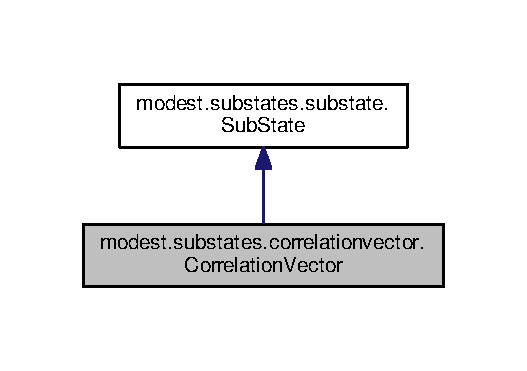
\includegraphics[width=253pt]{classmodest_1_1substates_1_1correlationvector_1_1CorrelationVector__inherit__graph}
\end{center}
\end{figure}


Collaboration diagram for modest.\+substates.\+correlationvector.\+Correlation\+Vector\+:
\nopagebreak
\begin{figure}[H]
\begin{center}
\leavevmode
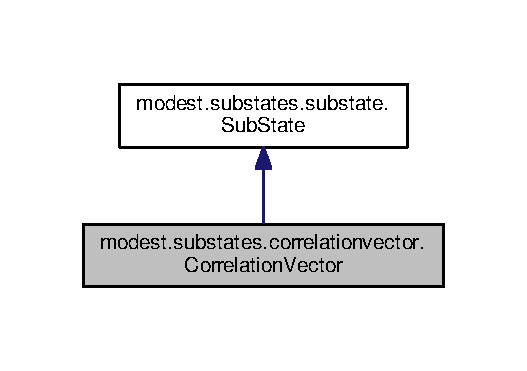
\includegraphics[width=253pt]{classmodest_1_1substates_1_1correlationvector_1_1CorrelationVector__coll__graph}
\end{center}
\end{figure}
\subsection*{Public Member Functions}
\begin{DoxyCompactItemize}
\item 
def \hyperlink{classmodest_1_1substates_1_1correlationvector_1_1CorrelationVector_ab344abe2451cdb5e476960cd3745eb62}{\+\_\+\+\_\+init\+\_\+\+\_\+} (self, true\+Signal, filter\+Order, dT, \hyperlink{classmodest_1_1substates_1_1correlationvector_1_1CorrelationVector_a127ca6c8eed6a2e822dbac7e83458bf3}{t}=0, \hyperlink{classmodest_1_1substates_1_1correlationvector_1_1CorrelationVector_a81da583ee9077067b6aaa354fd8a8c49}{correlation\+Vector}=None, \hyperlink{classmodest_1_1substates_1_1correlationvector_1_1CorrelationVector_a03bf36ec74d2fa70eeec14da348bec0c}{correlation\+Vector\+Covariance}=None, \hyperlink{classmodest_1_1substates_1_1correlationvector_1_1CorrelationVector_aa1565b9972d60149f335e3b923cac371}{signal\+Delay}=0, \hyperlink{classmodest_1_1substates_1_1correlationvector_1_1CorrelationVector_ab0c6ffbea793ae20593e85d033341595}{delay\+Var}=0, \hyperlink{classmodest_1_1substates_1_1correlationvector_1_1CorrelationVector_a9af2ca612576e52c84e98757e53085a8}{a\+Priori}=True, \hyperlink{classmodest_1_1substates_1_1correlationvector_1_1CorrelationVector_a9dbc1cdcfab963b133537b54f0a6d7a6}{center\+Peak}=True, \hyperlink{classmodest_1_1substates_1_1correlationvector_1_1CorrelationVector_af2be8d7129fd0453208af5268fdddc22}{peak\+Fit\+Points}=1, \hyperlink{classmodest_1_1substates_1_1correlationvector_1_1CorrelationVector_ab1756128cdec161ea22557d756745195}{process\+Noise}=1e-\/12, measurement\+Noise\+Scale\+Factor=1)
\begin{DoxyCompactList}\small\item\em \hyperlink{classmodest_1_1substates_1_1correlationvector_1_1CorrelationVector_ab344abe2451cdb5e476960cd3745eb62}{\+\_\+\+\_\+init\+\_\+\+\_\+} is responsible for initializing a correlation vector estimator \end{DoxyCompactList}\item 
def \hyperlink{classmodest_1_1substates_1_1correlationvector_1_1CorrelationVector_a3514ce57ec201ece8a5144f515d2d02c}{build\+Time\+Update\+Matrices} (self, deltaT, dynamics, h)
\begin{DoxyCompactList}\small\item\em \hyperlink{classmodest_1_1substates_1_1correlationvector_1_1CorrelationVector_a3514ce57ec201ece8a5144f515d2d02c}{build\+Time\+Update\+Matrices} constructs the correlation vector time update matrices \end{DoxyCompactList}\end{DoxyCompactItemize}
\begin{Indent}{\bf Mandatory Sub\+State Functions}\par
{\em The following functions are required in order for this class to be used as a substate in Modular\+Filter.

The inside of the functions may be changed or updated, but their \char`\"{}black box\char`\"{} behavior must remain the same; i.\+e. they must still perform the same essential functions and return the same things. }\begin{DoxyCompactItemize}
\item 
def \hyperlink{classmodest_1_1substates_1_1correlationvector_1_1CorrelationVector_a70ed47697f09424e62e52133fdfb59de}{store\+State\+Vector} (self, sv\+Dict)
\begin{DoxyCompactList}\small\item\em \hyperlink{classmodest_1_1substates_1_1correlationvector_1_1CorrelationVector_a70ed47697f09424e62e52133fdfb59de}{store\+State\+Vector} stores an updated estimate of the state vector \end{DoxyCompactList}\item 
def \hyperlink{classmodest_1_1substates_1_1correlationvector_1_1CorrelationVector_a59c13e5fa26ba27717494f687ec78ef8}{time\+Update} (self, dT, dynamics=None)
\begin{DoxyCompactList}\small\item\em \hyperlink{classmodest_1_1substates_1_1correlationvector_1_1CorrelationVector_a59c13e5fa26ba27717494f687ec78ef8}{time\+Update} returns the matrices for performing the correlation vector time update. \end{DoxyCompactList}\item 
def \hyperlink{classmodest_1_1substates_1_1correlationvector_1_1CorrelationVector_a2fb13d8c6fffa49ee641dd918a64db4b}{get\+Measurement\+Matrices} (self, measurement, source=None)
\begin{DoxyCompactList}\small\item\em \hyperlink{classmodest_1_1substates_1_1correlationvector_1_1CorrelationVector_a70ed47697f09424e62e52133fdfb59de}{store\+State\+Vector} stores an updated estimate of the state vector \end{DoxyCompactList}\end{DoxyCompactItemize}
\end{Indent}
\begin{Indent}{\bf Mandatory Sub\+State Functions}\par
{\em The following functions are functions which are required for the Sub\+State to function as a sub-\/state in State.\+Modular\+Filter. }\begin{DoxyCompactItemize}
\item 
def \hyperlink{classmodest_1_1substates_1_1substate_1_1SubState_aa18c8238415131b4b63cef0e4b2ff9fd}{get\+State\+Vector} (self)
\begin{DoxyCompactList}\small\item\em \hyperlink{classmodest_1_1substates_1_1substate_1_1SubState_aa18c8238415131b4b63cef0e4b2ff9fd}{get\+State\+Vector} returns the most recent value of the state vector \end{DoxyCompactList}\item 
def \hyperlink{classmodest_1_1substates_1_1substate_1_1SubState_a6e308aadd13962e476d2892ec728e3a5}{covariance} (self)
\begin{DoxyCompactList}\small\item\em \hyperlink{classmodest_1_1substates_1_1substate_1_1SubState_a6e308aadd13962e476d2892ec728e3a5}{covariance} returns the \hyperlink{classmodest_1_1substates_1_1substate_1_1SubState}{Sub\+State} covariance matrix \end{DoxyCompactList}\item 
def \hyperlink{classmodest_1_1substates_1_1substate_1_1SubState_ab9027f6d1d7d57c47731612f519b7ee6}{dimension} (self)
\begin{DoxyCompactList}\small\item\em \hyperlink{classmodest_1_1substates_1_1substate_1_1SubState_ab9027f6d1d7d57c47731612f519b7ee6}{dimension} returns the dimension of the sub-\/state vector \end{DoxyCompactList}\end{DoxyCompactItemize}
\end{Indent}
\begin{Indent}{\bf Plotting Functions}\par
{\em These functions provide generalized plotting capabilities }\begin{DoxyCompactItemize}
\item 
def \hyperlink{classmodest_1_1substates_1_1substate_1_1SubState_a1adac64be88eab0a64bb952518c4268f}{initialize\+Real\+Time\+Plot} (self, plot\+Handle=None, axis\+Handle=None)
\item 
def \hyperlink{classmodest_1_1substates_1_1substate_1_1SubState_a2deb7d1ca3105eb20e50fa7e67298355}{real\+Time\+Plot} (self, normalized=True)
\end{DoxyCompactItemize}
\end{Indent}
\subsection*{Public Attributes}
\begin{DoxyCompactItemize}
\item 
\hyperlink{classmodest_1_1substates_1_1correlationvector_1_1CorrelationVector_a127ca6c8eed6a2e822dbac7e83458bf3}{t}
\begin{DoxyCompactList}\small\item\em \hyperlink{classmodest_1_1substates_1_1correlationvector_1_1CorrelationVector_a127ca6c8eed6a2e822dbac7e83458bf3}{t} The current time \end{DoxyCompactList}\item 
\hyperlink{classmodest_1_1substates_1_1correlationvector_1_1CorrelationVector_a9af2ca612576e52c84e98757e53085a8}{a\+Priori}
\begin{DoxyCompactList}\small\item\em \hyperlink{classmodest_1_1substates_1_1correlationvector_1_1CorrelationVector_a9af2ca612576e52c84e98757e53085a8}{a\+Priori} Indicates whether the current state vector is the result of a time update (\hyperlink{classmodest_1_1substates_1_1correlationvector_1_1CorrelationVector_a9af2ca612576e52c84e98757e53085a8}{a\+Priori} = True) or a measurement update (\hyperlink{classmodest_1_1substates_1_1correlationvector_1_1CorrelationVector_a9af2ca612576e52c84e98757e53085a8}{a\+Priori} = False) \end{DoxyCompactList}\item 
\hyperlink{classmodest_1_1substates_1_1correlationvector_1_1CorrelationVector_a81da583ee9077067b6aaa354fd8a8c49}{correlation\+Vector}
\begin{DoxyCompactList}\small\item\em \hyperlink{classmodest_1_1substates_1_1correlationvector_1_1CorrelationVector_a81da583ee9077067b6aaa354fd8a8c49}{correlation\+Vector} is the current estimate of the correlation vector between the incoming signal measurements and the \hyperlink{classmodest_1_1substates_1_1correlationvector_1_1CorrelationVector_af2f52cea1c695f36dd100f529c322e94}{\+\_\+\+\_\+true\+Signal\+\_\+\+\_\+} \end{DoxyCompactList}\item 
\hyperlink{classmodest_1_1substates_1_1correlationvector_1_1CorrelationVector_a03bf36ec74d2fa70eeec14da348bec0c}{correlation\+Vector\+Covariance}
\begin{DoxyCompactList}\small\item\em \hyperlink{classmodest_1_1substates_1_1correlationvector_1_1CorrelationVector_a03bf36ec74d2fa70eeec14da348bec0c}{correlation\+Vector\+Covariance} is the covariance matrix of the correlation vector estimate, \hyperlink{classmodest_1_1substates_1_1correlationvector_1_1CorrelationVector_a81da583ee9077067b6aaa354fd8a8c49}{correlation\+Vector} \end{DoxyCompactList}\item 
\hyperlink{classmodest_1_1substates_1_1correlationvector_1_1CorrelationVector_aa1565b9972d60149f335e3b923cac371}{signal\+Delay}
\begin{DoxyCompactList}\small\item\em \hyperlink{classmodest_1_1substates_1_1correlationvector_1_1CorrelationVector_aa1565b9972d60149f335e3b923cac371}{signal\+Delay} is the current estimate of the delay between the incoming signal measurements and the \hyperlink{classmodest_1_1substates_1_1correlationvector_1_1CorrelationVector_af2f52cea1c695f36dd100f529c322e94}{\+\_\+\+\_\+true\+Signal\+\_\+\+\_\+} \end{DoxyCompactList}\item 
\hyperlink{classmodest_1_1substates_1_1correlationvector_1_1CorrelationVector_ab0c6ffbea793ae20593e85d033341595}{delay\+Var}
\begin{DoxyCompactList}\small\item\em \hyperlink{classmodest_1_1substates_1_1correlationvector_1_1CorrelationVector_ab0c6ffbea793ae20593e85d033341595}{delay\+Var} is the variance of the signal delay estimate \hyperlink{classmodest_1_1substates_1_1correlationvector_1_1CorrelationVector_aa1565b9972d60149f335e3b923cac371}{signal\+Delay} \end{DoxyCompactList}\item 
\hyperlink{classmodest_1_1substates_1_1correlationvector_1_1CorrelationVector_a9dbc1cdcfab963b133537b54f0a6d7a6}{center\+Peak}
\begin{DoxyCompactList}\small\item\em \hyperlink{classmodest_1_1substates_1_1correlationvector_1_1CorrelationVector_a9dbc1cdcfab963b133537b54f0a6d7a6}{center\+Peak} indicates whether the correlation vector is shifted to maintain the peak at the 0th tap \end{DoxyCompactList}\item 
\hyperlink{classmodest_1_1substates_1_1correlationvector_1_1CorrelationVector_af2be8d7129fd0453208af5268fdddc22}{peak\+Fit\+Points}
\begin{DoxyCompactList}\small\item\em \hyperlink{classmodest_1_1substates_1_1correlationvector_1_1CorrelationVector_af2be8d7129fd0453208af5268fdddc22}{peak\+Fit\+Points} is a variable which controls the number of points used for quadratically estimating the location of the correlation vector peak \end{DoxyCompactList}\item 
\hyperlink{classmodest_1_1substates_1_1correlationvector_1_1CorrelationVector_ab1756128cdec161ea22557d756745195}{process\+Noise}
\begin{DoxyCompactList}\small\item\em \hyperlink{classmodest_1_1substates_1_1correlationvector_1_1CorrelationVector_ab1756128cdec161ea22557d756745195}{process\+Noise} is the scalar value used to generate an additional process noise term in \hyperlink{classmodest_1_1substates_1_1correlationvector_1_1CorrelationVector_a59c13e5fa26ba27717494f687ec78ef8}{time\+Update}. \end{DoxyCompactList}\item 
\hyperlink{classmodest_1_1substates_1_1correlationvector_1_1CorrelationVector_ae1c71753aea17170b58bd9fabc62c037}{measurement\+Noise\+Scale\+Factor}
\begin{DoxyCompactList}\small\item\em \hyperlink{classmodest_1_1substates_1_1correlationvector_1_1CorrelationVector_ae1c71753aea17170b58bd9fabc62c037}{measurement\+Noise\+Scale\+Factor} is a factor used to scale the measurement noise matrix. \end{DoxyCompactList}\item 
\hyperlink{classmodest_1_1substates_1_1substate_1_1SubState_a38c12c9d0899bc1161f3502b584517a2}{state\+Vector\+History}
\begin{DoxyCompactList}\small\item\em Stores the time-\/history of the sub-\/state state vector. \end{DoxyCompactList}\item 
\hyperlink{classmodest_1_1substates_1_1substate_1_1SubState_a37ded775b84cea85b4dce0f1b16286c4}{R\+T\+Plot\+Handle}
\begin{DoxyCompactList}\small\item\em Stores handle for real-\/time plotting. \end{DoxyCompactList}\item 
\hyperlink{classmodest_1_1substates_1_1substate_1_1SubState_a9fefae1facc797a1132fb61a55e9ffa1}{R\+T\+Plot\+Data}
\item 
\hyperlink{classmodest_1_1substates_1_1substate_1_1SubState_a497ccbb6658589b02568e87c6382222e}{R\+T\+Paxis\+Handle}
\end{DoxyCompactItemize}
\subsection*{Private Attributes}
\begin{DoxyCompactItemize}
\item 
\hyperlink{classmodest_1_1substates_1_1correlationvector_1_1CorrelationVector_a4a6aacd90c573941e4f097a034bdb76c}{\+\_\+\+\_\+unit\+Vec\+To\+Signal\+\_\+\+\_\+}
\begin{DoxyCompactList}\small\item\em \hyperlink{classmodest_1_1substates_1_1correlationvector_1_1CorrelationVector_a4a6aacd90c573941e4f097a034bdb76c}{\+\_\+\+\_\+unit\+Vec\+To\+Signal\+\_\+\+\_\+} is a unit vector which points to the signal source \end{DoxyCompactList}\item 
\hyperlink{classmodest_1_1substates_1_1correlationvector_1_1CorrelationVector_af2f52cea1c695f36dd100f529c322e94}{\+\_\+\+\_\+true\+Signal\+\_\+\+\_\+}
\begin{DoxyCompactList}\small\item\em \hyperlink{classmodest_1_1substates_1_1correlationvector_1_1CorrelationVector_af2f52cea1c695f36dd100f529c322e94}{\+\_\+\+\_\+true\+Signal\+\_\+\+\_\+} is a signal object that contains the \char`\"{}true\char`\"{} signal for which the correlation vector is being estimated \end{DoxyCompactList}\item 
\hyperlink{classmodest_1_1substates_1_1correlationvector_1_1CorrelationVector_a6454cf8c143629a28cf684f6abbf4830}{\+\_\+\+\_\+filter\+Order\+\_\+\+\_\+}
\begin{DoxyCompactList}\small\item\em \hyperlink{classmodest_1_1substates_1_1correlationvector_1_1CorrelationVector_a6454cf8c143629a28cf684f6abbf4830}{\+\_\+\+\_\+filter\+Order\+\_\+\+\_\+} is the number of \char`\"{}taps\char`\"{} in the estimated correlation vector, \hyperlink{classmodest_1_1substates_1_1correlationvector_1_1CorrelationVector_a81da583ee9077067b6aaa354fd8a8c49}{correlation\+Vector}. \end{DoxyCompactList}\item 
\hyperlink{classmodest_1_1substates_1_1correlationvector_1_1CorrelationVector_a402e91c0356dd1a8b778916eec7bdd86}{\+\_\+\+\_\+d\+T\+\_\+\+\_\+}
\begin{DoxyCompactList}\small\item\em \hyperlink{classmodest_1_1substates_1_1correlationvector_1_1CorrelationVector_a402e91c0356dd1a8b778916eec7bdd86}{\+\_\+\+\_\+d\+T\+\_\+\+\_\+} is the \char`\"{}sample period\char`\"{} or \char`\"{}bin size\char`\"{} of the estimated correlation vector \end{DoxyCompactList}\end{DoxyCompactItemize}
\subsection*{Functions Specific to \#Correlation\+Vector}
\label{_amgrpb77571167b4af2d56b573fb28e024ebf}%
The following remaining functions are not required in order for this class to be used as a Sub\+State, and may be changed as needed, including inputs and outputs.\begin{DoxyCompactItemize}
\item 
def \hyperlink{classmodest_1_1substates_1_1correlationvector_1_1CorrelationVector_a71f11fa45819ecb464890be81ecc9781}{get\+T\+O\+A\+Measurement\+Matrices} (self, measurement, corr\+Vec)
\begin{DoxyCompactList}\small\item\em \hyperlink{classmodest_1_1substates_1_1correlationvector_1_1CorrelationVector_a0d0188e2923b59ba3e620927f1aaf84a}{compute\+Signal\+Delay} computes the delay between the \hyperlink{classmodest_1_1substates_1_1correlationvector_1_1CorrelationVector_af2f52cea1c695f36dd100f529c322e94}{\+\_\+\+\_\+true\+Signal\+\_\+\+\_\+} and measurements based on a correlation vector \end{DoxyCompactList}\item 
def \hyperlink{classmodest_1_1substates_1_1correlationvector_1_1CorrelationVector_a0d0188e2923b59ba3e620927f1aaf84a}{compute\+Signal\+Delay} (self, c, P)
\begin{DoxyCompactList}\small\item\em \hyperlink{classmodest_1_1substates_1_1correlationvector_1_1CorrelationVector_a0d0188e2923b59ba3e620927f1aaf84a}{compute\+Signal\+Delay} computes the delay between the \hyperlink{classmodest_1_1substates_1_1correlationvector_1_1CorrelationVector_af2f52cea1c695f36dd100f529c322e94}{\+\_\+\+\_\+true\+Signal\+\_\+\+\_\+} and measurements based on a correlation vector \end{DoxyCompactList}\item 
def \hyperlink{classmodest_1_1substates_1_1correlationvector_1_1CorrelationVector_a7bd7d1e68287728a48a414440c55c988}{estimate\+Signal\+Delay\+UT} (self, h, P)
\begin{DoxyCompactList}\small\item\em \hyperlink{classmodest_1_1substates_1_1correlationvector_1_1CorrelationVector_a7bd7d1e68287728a48a414440c55c988}{estimate\+Signal\+Delay\+UT} uses a unscented tranform to estimate the delay corresponding to a correlation vector \end{DoxyCompactList}\item 
def \hyperlink{classmodest_1_1substates_1_1correlationvector_1_1CorrelationVector_a5b95e0a827fb233f2f1a40f2cff9d3f0}{speed\+Of\+Light} (self)
\begin{DoxyCompactList}\small\item\em \hyperlink{classmodest_1_1substates_1_1correlationvector_1_1CorrelationVector_a0d0188e2923b59ba3e620927f1aaf84a}{compute\+Signal\+Delay} computes the delay between the \hyperlink{classmodest_1_1substates_1_1correlationvector_1_1CorrelationVector_af2f52cea1c695f36dd100f529c322e94}{\+\_\+\+\_\+true\+Signal\+\_\+\+\_\+} and measurements based on a correlation vector \end{DoxyCompactList}\item 
def \hyperlink{classmodest_1_1substates_1_1correlationvector_1_1CorrelationVector_a033e07143d7a0aeefb3136d42a380ee3}{sinc\+Diff} (x)
\begin{DoxyCompactList}\small\item\em \hyperlink{classmodest_1_1substates_1_1correlationvector_1_1CorrelationVector_a0d0188e2923b59ba3e620927f1aaf84a}{compute\+Signal\+Delay} computes the delay between the \hyperlink{classmodest_1_1substates_1_1correlationvector_1_1CorrelationVector_af2f52cea1c695f36dd100f529c322e94}{\+\_\+\+\_\+true\+Signal\+\_\+\+\_\+} and measurements based on a correlation vector \end{DoxyCompactList}\end{DoxyCompactItemize}


\subsection{Detailed Description}
\hyperlink{classmodest_1_1substates_1_1correlationvector_1_1CorrelationVector}{Correlation\+Vector} estimates the correlation vector and delay between a signal and a time-\/delayed measurement of that signal. 

This class contains an estimator which estimates the correlation vector between a signal (the \hyperlink{classmodest_1_1substates_1_1correlationvector_1_1CorrelationVector_af2f52cea1c695f36dd100f529c322e94}{\+\_\+\+\_\+true\+Signal\+\_\+\+\_\+}) and measurements of that signal. This correlation vector is then used to estimate the delay between the \hyperlink{classmodest_1_1substates_1_1correlationvector_1_1CorrelationVector_af2f52cea1c695f36dd100f529c322e94}{\+\_\+\+\_\+true\+Signal\+\_\+\+\_\+} and the measurements of that signal.

The estimator in this class currently assumes that the signal source is \char`\"{}distant,\char`\"{} or infinitely far away. This implies that the unit vector to the signal source is perfectly known, and not changing. A later implementation could include the option of having a non-\/distant signal source, in which the unit vector is changing as a function of position and therefore uncertain.

\begin{DoxyNote}{Note}
This class is essentially an implementation of the estimator presented in \href{https://doi.org/10.2514/1.G002650}{\tt Recursive Range Estimation Using Astrophysical Signals of Opportunity}, J. Runnels, D. Gebre, Journal of Guidance, Control and Dynamics, 2017. Some equations from the paper are included in the class documentation for reference. A more detailed discussion and derivation of the estimator can be found in the journal article.. 
\end{DoxyNote}


Definition at line 36 of file correlationvector.\+py.



\subsection{Constructor \& Destructor Documentation}
\index{modest\+::substates\+::correlationvector\+::\+Correlation\+Vector@{modest\+::substates\+::correlationvector\+::\+Correlation\+Vector}!\+\_\+\+\_\+init\+\_\+\+\_\+@{\+\_\+\+\_\+init\+\_\+\+\_\+}}
\index{\+\_\+\+\_\+init\+\_\+\+\_\+@{\+\_\+\+\_\+init\+\_\+\+\_\+}!modest\+::substates\+::correlationvector\+::\+Correlation\+Vector@{modest\+::substates\+::correlationvector\+::\+Correlation\+Vector}}
\subsubsection[{\texorpdfstring{\+\_\+\+\_\+init\+\_\+\+\_\+(self, true\+Signal, filter\+Order, d\+T, t=0, correlation\+Vector=\+None, correlation\+Vector\+Covariance=\+None, signal\+Delay=0, delay\+Var=0, a\+Priori=\+True, center\+Peak=\+True, peak\+Fit\+Points=1, process\+Noise=1e-\/12, measurement\+Noise\+Scale\+Factor=1)}{__init__(self, trueSignal, filterOrder, dT, t=0, correlationVector=None, correlationVectorCovariance=None, signalDelay=0, delayVar=0, aPriori=True, centerPeak=True, peakFitPoints=1, processNoise=1e-12, measurementNoiseScaleFactor=1)}}]{\setlength{\rightskip}{0pt plus 5cm}def modest.\+substates.\+correlationvector.\+Correlation\+Vector.\+\_\+\+\_\+init\+\_\+\+\_\+ (
\begin{DoxyParamCaption}
\item[{}]{self, }
\item[{}]{true\+Signal, }
\item[{}]{filter\+Order, }
\item[{}]{dT, }
\item[{}]{t = {\ttfamily 0}, }
\item[{}]{correlation\+Vector = {\ttfamily None}, }
\item[{}]{correlation\+Vector\+Covariance = {\ttfamily None}, }
\item[{}]{signal\+Delay = {\ttfamily 0}, }
\item[{}]{delay\+Var = {\ttfamily 0}, }
\item[{}]{a\+Priori = {\ttfamily True}, }
\item[{}]{center\+Peak = {\ttfamily True}, }
\item[{}]{peak\+Fit\+Points = {\ttfamily 1}, }
\item[{}]{process\+Noise = {\ttfamily 1e-\/12}, }
\item[{}]{measurement\+Noise\+Scale\+Factor = {\ttfamily 1}}
\end{DoxyParamCaption}
)}\hypertarget{classmodest_1_1substates_1_1correlationvector_1_1CorrelationVector_ab344abe2451cdb5e476960cd3745eb62}{}\label{classmodest_1_1substates_1_1correlationvector_1_1CorrelationVector_ab344abe2451cdb5e476960cd3745eb62}


\hyperlink{classmodest_1_1substates_1_1correlationvector_1_1CorrelationVector_ab344abe2451cdb5e476960cd3745eb62}{\+\_\+\+\_\+init\+\_\+\+\_\+} is responsible for initializing a correlation vector estimator 

The primary function of the \hyperlink{classmodest_1_1substates_1_1correlationvector_1_1CorrelationVector_ab344abe2451cdb5e476960cd3745eb62}{\+\_\+\+\_\+init\+\_\+\+\_\+} method is to initialize the correlation vector estimator, and store the relevant user inputs. A few key user inputs are required in order to initialize the filter. Additionally, because the algorithm is relatively complicated, there are a number of optional tuning parameters which may be inputed at initialization.

In general, the parameters which are required inputs are the ones that are critical for initialization of the filter, and should not be changed during the course of the filter\textquotesingle{}s lifetime. These inputs are stored as \char`\"{}private\char`\"{} variables; indicating that the should not be changed during the object\textquotesingle{}s lifetime.

The optional inputs, on the other hand, are inputs which are used in the estimation functions (\hyperlink{classmodest_1_1substates_1_1correlationvector_1_1CorrelationVector_a59c13e5fa26ba27717494f687ec78ef8}{time\+Update}, \hyperlink{classmodest_1_1substates_1_1correlationvector_1_1CorrelationVector_a2fb13d8c6fffa49ee641dd918a64db4b}{get\+Measurement\+Matrices}, etc.). These parameters could conceivably be changed during the lifetime of the filter without causing problems, and the user may want to change them depending on external factors. These parameters are initalized with default values, and stored as public variables that the user can in theory change.

There are also a set of class variables which are publicly accessable and which hold the most recent state estimate. These exist primarily for convenience, and are never actually used within the class. Modifying them will have no affect on the state estimates. The only way to modify a state estimate is through the \hyperlink{classmodest_1_1substates_1_1correlationvector_1_1CorrelationVector_a70ed47697f09424e62e52133fdfb59de}{store\+State\+Vector} method.

The \hyperlink{classmodest_1_1substates_1_1correlationvector_1_1CorrelationVector_ab344abe2451cdb5e476960cd3745eb62}{\+\_\+\+\_\+init\+\_\+\+\_\+} method also checks the user inputs to ensure that they are consistent with how they will be used in the class (where applicable).

The true\+Signal input is checked to see whether it has the following methods\+:
\begin{DoxyItemize}
\item flux()
\item peak\+Amplitude()
\item signal\+I\+D()
\item unit\+Vec()
\end{DoxyItemize}


\begin{DoxyParams}[1]{Parameters}
 & {\em true\+Signal} & An object that describes the signal for which correlation should be estimated. \\
\hline
 & {\em filter\+Order} & The number of bins or \char`\"{}taps\char`\"{} in the correlation vector \\
\hline
 & {\em dT} & The sampling period, or time-\/step between bins in the correlation vector\\
\hline
 & {\em t} & (optional) The initial starting time. If no value is passed, initialized to zero by default. \\
\hline
 & {\em correlation\+Vector} & (optional) The initial value of the correlation vector. If not supplied, the correlation vector will be initialized based on the filter \hyperlink{classmodest_1_1substates_1_1correlationvector_1_1CorrelationVector_a402e91c0356dd1a8b778916eec7bdd86}{\+\_\+\+\_\+d\+T\+\_\+\+\_\+} and maximum flux of the \hyperlink{classmodest_1_1substates_1_1correlationvector_1_1CorrelationVector_af2f52cea1c695f36dd100f529c322e94}{\+\_\+\+\_\+true\+Signal\+\_\+\+\_\+}. \\
\hline
 & {\em correlation\+Vector\+Covariance} & (optional) The initial value of the correlation vector estimate covariance. If not supplied, the covariance matrix will be initialized based on the filter \hyperlink{classmodest_1_1substates_1_1correlationvector_1_1CorrelationVector_a402e91c0356dd1a8b778916eec7bdd86}{\+\_\+\+\_\+d\+T\+\_\+\+\_\+} and maximum flux of \hyperlink{classmodest_1_1substates_1_1correlationvector_1_1CorrelationVector_af2f52cea1c695f36dd100f529c322e94}{\+\_\+\+\_\+true\+Signal\+\_\+\+\_\+}. \\
\hline
 & {\em signal\+Delay} & (optional) The initial estimate of delay between the \hyperlink{classmodest_1_1substates_1_1correlationvector_1_1CorrelationVector_af2f52cea1c695f36dd100f529c322e94}{\+\_\+\+\_\+true\+Signal\+\_\+\+\_\+} and the signal measurements. If not supplied, \hyperlink{classmodest_1_1substates_1_1correlationvector_1_1CorrelationVector_aa1565b9972d60149f335e3b923cac371}{signal\+Delay} is initialized to zero. \\
\hline
 & {\em delay\+Var} & (optional) The variance of the estimate of delay \\
\hline
 & {\em a\+Priori} & (optional) Indicates whether initial estimates are a priori or a posteriori. Default=True\\
\hline
 & {\em center\+Peak} & (optional) Boolean indicating whether the correlation vector should be \char`\"{}shifted\char`\"{} after each update to keep the peak centered at the zero index. Default is True. \\
\hline
 & {\em peak\+Fit\+Points} & (optional) Number of points used on either side of max for quadratic fit in \hyperlink{classmodest_1_1substates_1_1correlationvector_1_1CorrelationVector_a0d0188e2923b59ba3e620927f1aaf84a}{compute\+Signal\+Delay}. Minimum is 1, default is 1. \\
\hline
 & {\em process\+Noise} & (optional) Scalar term of additional process noise added to covariance matrix in time update. Default is 1e-\/12 \\
\hline
 & {\em measurement\+Noise\+Scale\+Factor} & (optional) Scale factor to inflate the measurement noise. Default is 1. \\
\hline
\end{DoxyParams}


Definition at line 125 of file correlationvector.\+py.



\subsection{Member Function Documentation}
\index{modest\+::substates\+::correlationvector\+::\+Correlation\+Vector@{modest\+::substates\+::correlationvector\+::\+Correlation\+Vector}!build\+Time\+Update\+Matrices@{build\+Time\+Update\+Matrices}}
\index{build\+Time\+Update\+Matrices@{build\+Time\+Update\+Matrices}!modest\+::substates\+::correlationvector\+::\+Correlation\+Vector@{modest\+::substates\+::correlationvector\+::\+Correlation\+Vector}}
\subsubsection[{\texorpdfstring{build\+Time\+Update\+Matrices(self, delta\+T, dynamics, h)}{buildTimeUpdateMatrices(self, deltaT, dynamics, h)}}]{\setlength{\rightskip}{0pt plus 5cm}def modest.\+substates.\+correlationvector.\+Correlation\+Vector.\+build\+Time\+Update\+Matrices (
\begin{DoxyParamCaption}
\item[{}]{self, }
\item[{}]{deltaT, }
\item[{}]{dynamics, }
\item[{}]{h}
\end{DoxyParamCaption}
)}\hypertarget{classmodest_1_1substates_1_1correlationvector_1_1CorrelationVector_a3514ce57ec201ece8a5144f515d2d02c}{}\label{classmodest_1_1substates_1_1correlationvector_1_1CorrelationVector_a3514ce57ec201ece8a5144f515d2d02c}


\hyperlink{classmodest_1_1substates_1_1correlationvector_1_1CorrelationVector_a3514ce57ec201ece8a5144f515d2d02c}{build\+Time\+Update\+Matrices} constructs the correlation vector time update matrices 

The \hyperlink{classmodest_1_1substates_1_1correlationvector_1_1CorrelationVector_a3514ce57ec201ece8a5144f515d2d02c}{build\+Time\+Update\+Matrices} method constructs the matrices required to perform the time update of the correlation vector sub-\/state.

The time update matrices are a function of the estimated spacecraft velocity ( $\mathbf{v}$), velocity variance ( $\mathbf{P}_{\mathbf{v}}$), and the elapsed time over which the time update occurs ( $\Delta T$). The matrices are constructed as follows\+:

\[ \mathbf{F}_{j \to k} = \begin{bmatrix} \textrm{sinc}(\hat{\delta}) & \hdots & \textrm{sinc}(\hat{\delta} + N - 1) \\ \vdots & \ddots & \vdots \\ \textrm{sinc}(\hat{\delta} - N + 1) & \hdots & \textrm{sinc}(\hat{\delta}) \end{bmatrix} \]

\[ \mathbf{L}_{j} = \begin{bmatrix} \frac{\textrm{cos}}{(\hat{\delta})} - \frac{\textrm{sin}}{(\hat{\delta}^2)} & \hdots \\ \vdots & \ddots \\ \end{bmatrix} \sv[timeIndex = k] \]

\[ Q_{\delta} = \left(\frac{(k-j)}{c}\right)^2 {\LOSVec[S]}^T \mathbf{P}_{\mathbf{v}} \LOSVec[S] \]

where

\[ \hat{\delta}_{j \to k} = \frac{\mathbf{v} \LOSVec[S] \Delta T}{c T} \]


\begin{DoxyParams}{Parameters}
{\em self} & The object pointer \\
\hline
{\em deltaT} & The amount of time over which the time update is occuring \\
\hline
{\em dynamics} & A dictionary containing the relevant dynamics for the time update \\
\hline
{\em h} & The current correlation vector\\
\hline
\end{DoxyParams}
\begin{DoxyReturn}{Returns}
A dictionary containing the matrices $\mathbf{F}$, $\mathbf{L}$, and the scalar 
\end{DoxyReturn}


Definition at line 353 of file correlationvector.\+py.

\index{modest\+::substates\+::correlationvector\+::\+Correlation\+Vector@{modest\+::substates\+::correlationvector\+::\+Correlation\+Vector}!compute\+Signal\+Delay@{compute\+Signal\+Delay}}
\index{compute\+Signal\+Delay@{compute\+Signal\+Delay}!modest\+::substates\+::correlationvector\+::\+Correlation\+Vector@{modest\+::substates\+::correlationvector\+::\+Correlation\+Vector}}
\subsubsection[{\texorpdfstring{compute\+Signal\+Delay(self, c, P)}{computeSignalDelay(self, c, P)}}]{\setlength{\rightskip}{0pt plus 5cm}def modest.\+substates.\+correlationvector.\+Correlation\+Vector.\+compute\+Signal\+Delay (
\begin{DoxyParamCaption}
\item[{}]{self, }
\item[{}]{c, }
\item[{}]{P}
\end{DoxyParamCaption}
)}\hypertarget{classmodest_1_1substates_1_1correlationvector_1_1CorrelationVector_a0d0188e2923b59ba3e620927f1aaf84a}{}\label{classmodest_1_1substates_1_1correlationvector_1_1CorrelationVector_a0d0188e2923b59ba3e620927f1aaf84a}


\hyperlink{classmodest_1_1substates_1_1correlationvector_1_1CorrelationVector_a0d0188e2923b59ba3e620927f1aaf84a}{compute\+Signal\+Delay} computes the delay between the \hyperlink{classmodest_1_1substates_1_1correlationvector_1_1CorrelationVector_af2f52cea1c695f36dd100f529c322e94}{\+\_\+\+\_\+true\+Signal\+\_\+\+\_\+} and measurements based on a correlation vector 

The \hyperlink{classmodest_1_1substates_1_1correlationvector_1_1CorrelationVector_a0d0188e2923b59ba3e620927f1aaf84a}{compute\+Signal\+Delay} function is a rudimentary function which takes an estimate of the correlation vector and uses it to estimate the location of the peak. It functions by finding the tap with the maximum value, and then fitting a quadratic to the points surrounding the maximum value tap. The number of points to which the quadratic is fitted is determined by the value of \hyperlink{classmodest_1_1substates_1_1correlationvector_1_1CorrelationVector_af2be8d7129fd0453208af5268fdddc22}{peak\+Fit\+Points}; the number of points is equal to $2 * n + 1$ where $n = $ \hyperlink{classmodest_1_1substates_1_1correlationvector_1_1CorrelationVector_af2be8d7129fd0453208af5268fdddc22}{peak\+Fit\+Points}.

The delay estimate that is returned is in units of \hyperlink{classmodest_1_1substates_1_1correlationvector_1_1CorrelationVector_a402e91c0356dd1a8b778916eec7bdd86}{\+\_\+\+\_\+d\+T\+\_\+\+\_\+}. So, a returned value of 2 would imply that the peak is located at 2, and therefore the delay corresponding to the correlation vector is 2 \hyperlink{classmodest_1_1substates_1_1correlationvector_1_1CorrelationVector_a402e91c0356dd1a8b778916eec7bdd86}{\+\_\+\+\_\+d\+T\+\_\+\+\_\+}.

The returned delay may not include previously accumulated \hyperlink{classmodest_1_1substates_1_1correlationvector_1_1CorrelationVector_aa1565b9972d60149f335e3b923cac371}{signal\+Delay} between the signal and the measurements. See the \hyperlink{classmodest_1_1substates_1_1correlationvector_1_1CorrelationVector_a70ed47697f09424e62e52133fdfb59de}{store\+State\+Vector} function for more information on how the \hyperlink{classmodest_1_1substates_1_1correlationvector_1_1CorrelationVector_aa1565b9972d60149f335e3b923cac371}{signal\+Delay} is stored and accumulated delay is accounted for.


\begin{DoxyParams}{Parameters}
{\em self} & The object pointer \\
\hline
{\em c} & The correlation vector \\
\hline
{\em P} & the correlation vector covariance matrix\\
\hline
\end{DoxyParams}
\begin{DoxyReturn}{Returns}
The estimate of the delay 
\end{DoxyReturn}


Definition at line 509 of file correlationvector.\+py.

\index{modest\+::substates\+::correlationvector\+::\+Correlation\+Vector@{modest\+::substates\+::correlationvector\+::\+Correlation\+Vector}!covariance@{covariance}}
\index{covariance@{covariance}!modest\+::substates\+::correlationvector\+::\+Correlation\+Vector@{modest\+::substates\+::correlationvector\+::\+Correlation\+Vector}}
\subsubsection[{\texorpdfstring{covariance(self)}{covariance(self)}}]{\setlength{\rightskip}{0pt plus 5cm}def modest.\+substates.\+substate.\+Sub\+State.\+covariance (
\begin{DoxyParamCaption}
\item[{}]{self}
\end{DoxyParamCaption}
)\hspace{0.3cm}{\ttfamily [inherited]}}\hypertarget{classmodest_1_1substates_1_1substate_1_1SubState_a6e308aadd13962e476d2892ec728e3a5}{}\label{classmodest_1_1substates_1_1substate_1_1SubState_a6e308aadd13962e476d2892ec728e3a5}


\hyperlink{classmodest_1_1substates_1_1substate_1_1SubState_a6e308aadd13962e476d2892ec728e3a5}{covariance} returns the \hyperlink{classmodest_1_1substates_1_1substate_1_1SubState}{Sub\+State} covariance matrix 

The \hyperlink{classmodest_1_1substates_1_1substate_1_1SubState_a6e308aadd13962e476d2892ec728e3a5}{covariance} method returns the covariance of the estimate of the substate.

\begin{DoxyRefDesc}{Todo}
\item[\hyperlink{todo__todo000001}{Todo}]Currently, this method only returns the covariance of the most recent state estimate. Ideally, there should be an optional time parameter which would allow the user to get the covaraince matrix at a specified time (or the closest to that specified time).\end{DoxyRefDesc}



\begin{DoxyParams}{Parameters}
{\em self} & The object pointer\\
\hline
\end{DoxyParams}
\begin{DoxyReturn}{Returns}
Returns the covaraince matrix 
\end{DoxyReturn}


Definition at line 173 of file substate.\+py.

\index{modest\+::substates\+::correlationvector\+::\+Correlation\+Vector@{modest\+::substates\+::correlationvector\+::\+Correlation\+Vector}!dimension@{dimension}}
\index{dimension@{dimension}!modest\+::substates\+::correlationvector\+::\+Correlation\+Vector@{modest\+::substates\+::correlationvector\+::\+Correlation\+Vector}}
\subsubsection[{\texorpdfstring{dimension(self)}{dimension(self)}}]{\setlength{\rightskip}{0pt plus 5cm}def modest.\+substates.\+substate.\+Sub\+State.\+dimension (
\begin{DoxyParamCaption}
\item[{}]{self}
\end{DoxyParamCaption}
)\hspace{0.3cm}{\ttfamily [inherited]}}\hypertarget{classmodest_1_1substates_1_1substate_1_1SubState_ab9027f6d1d7d57c47731612f519b7ee6}{}\label{classmodest_1_1substates_1_1substate_1_1SubState_ab9027f6d1d7d57c47731612f519b7ee6}


\hyperlink{classmodest_1_1substates_1_1substate_1_1SubState_ab9027f6d1d7d57c47731612f519b7ee6}{dimension} returns the dimension of the sub-\/state vector 

The \hyperlink{classmodest_1_1substates_1_1substate_1_1SubState_ab9027f6d1d7d57c47731612f519b7ee6}{dimension} method returns the dimension of the sub-\/state vector estimated by the \hyperlink{classmodest_1_1substates_1_1substate_1_1SubState}{Sub\+State}. This is the dimension as seen by the Modular\+Filter estimator.

The default implementation is to return the class variable \hyperlink{classmodest_1_1substates_1_1substate_1_1SubState_a5b1c0756a69da7f293a415c7d2d77843}{\+\_\+\+\_\+dimension\+\_\+\+\_\+}, which is saved at initialization. This is designated as a \char`\"{}protected\char`\"{} variable, and should not change during the course of the \hyperlink{classmodest_1_1substates_1_1substate_1_1SubState}{Sub\+State}\textquotesingle{}s lifetime. If child class overwrites this implementation, care should be taken to ensure that the value returned by \hyperlink{classmodest_1_1substates_1_1substate_1_1SubState_ab9027f6d1d7d57c47731612f519b7ee6}{dimension} does not change over \hyperlink{classmodest_1_1substates_1_1substate_1_1SubState}{Sub\+State} object lifetime.

For \hyperlink{classmodest_1_1substates_1_1substate_1_1SubState}{Sub\+State} objects with auxilary states, or other quantities related to the state vector but not directly estimated by the Modular\+Filter, \hyperlink{classmodest_1_1substates_1_1substate_1_1SubState_ab9027f6d1d7d57c47731612f519b7ee6}{dimension} should not count these states as part of the total dimension.


\begin{DoxyParams}{Parameters}
{\em self} & The object pointer\\
\hline
\end{DoxyParams}
\begin{DoxyReturn}{Returns}
Returns the dimension of state vector 
\end{DoxyReturn}


Definition at line 198 of file substate.\+py.

\index{modest\+::substates\+::correlationvector\+::\+Correlation\+Vector@{modest\+::substates\+::correlationvector\+::\+Correlation\+Vector}!estimate\+Signal\+Delay\+UT@{estimate\+Signal\+Delay\+UT}}
\index{estimate\+Signal\+Delay\+UT@{estimate\+Signal\+Delay\+UT}!modest\+::substates\+::correlationvector\+::\+Correlation\+Vector@{modest\+::substates\+::correlationvector\+::\+Correlation\+Vector}}
\subsubsection[{\texorpdfstring{estimate\+Signal\+Delay\+U\+T(self, h, P)}{estimateSignalDelayUT(self, h, P)}}]{\setlength{\rightskip}{0pt plus 5cm}def modest.\+substates.\+correlationvector.\+Correlation\+Vector.\+estimate\+Signal\+Delay\+UT (
\begin{DoxyParamCaption}
\item[{}]{self, }
\item[{}]{h, }
\item[{}]{P}
\end{DoxyParamCaption}
)}\hypertarget{classmodest_1_1substates_1_1correlationvector_1_1CorrelationVector_a7bd7d1e68287728a48a414440c55c988}{}\label{classmodest_1_1substates_1_1correlationvector_1_1CorrelationVector_a7bd7d1e68287728a48a414440c55c988}


\hyperlink{classmodest_1_1substates_1_1correlationvector_1_1CorrelationVector_a7bd7d1e68287728a48a414440c55c988}{estimate\+Signal\+Delay\+UT} uses a unscented tranform to estimate the delay corresponding to a correlation vector 

The \hyperlink{classmodest_1_1substates_1_1correlationvector_1_1CorrelationVector_a7bd7d1e68287728a48a414440c55c988}{estimate\+Signal\+Delay\+UT} method is responsible for computing the estimated value of delay corresponding to a correlation vector, as well as the variance of that estimate. These values are computed using a unscented transform (i.\+e. sigma-\/point) approach.

The method receives the an estimate of the correlation vector, as well as the covariance matrix corresponding to that vector. From there it computes a set of n sigma points (where n is the length of the correlation vector), and for each of the generated sigma point vectors, it computes the peak location using the \hyperlink{classmodest_1_1substates_1_1correlationvector_1_1CorrelationVector_a0d0188e2923b59ba3e620927f1aaf84a}{compute\+Signal\+Delay} method.


\begin{DoxyParams}{Parameters}
{\em self} & The object pointer \\
\hline
{\em h} & The correlation vector \\
\hline
{\em P} & The correlation vector covariance matrix\\
\hline
\end{DoxyParams}
\begin{DoxyReturn}{Returns}
A dict containing the estimate of the peak location (\char`\"{}mean\+Delay\char`\"{}) and the estimate variance (\char`\"{}var\+Delay\char`\"{}) 
\end{DoxyReturn}


Definition at line 584 of file correlationvector.\+py.

\index{modest\+::substates\+::correlationvector\+::\+Correlation\+Vector@{modest\+::substates\+::correlationvector\+::\+Correlation\+Vector}!get\+Measurement\+Matrices@{get\+Measurement\+Matrices}}
\index{get\+Measurement\+Matrices@{get\+Measurement\+Matrices}!modest\+::substates\+::correlationvector\+::\+Correlation\+Vector@{modest\+::substates\+::correlationvector\+::\+Correlation\+Vector}}
\subsubsection[{\texorpdfstring{get\+Measurement\+Matrices(self, measurement, source=\+None)}{getMeasurementMatrices(self, measurement, source=None)}}]{\setlength{\rightskip}{0pt plus 5cm}def modest.\+substates.\+correlationvector.\+Correlation\+Vector.\+get\+Measurement\+Matrices (
\begin{DoxyParamCaption}
\item[{}]{self, }
\item[{}]{measurement, }
\item[{}]{source = {\ttfamily None}}
\end{DoxyParamCaption}
)}\hypertarget{classmodest_1_1substates_1_1correlationvector_1_1CorrelationVector_a2fb13d8c6fffa49ee641dd918a64db4b}{}\label{classmodest_1_1substates_1_1correlationvector_1_1CorrelationVector_a2fb13d8c6fffa49ee641dd918a64db4b}


\hyperlink{classmodest_1_1substates_1_1correlationvector_1_1CorrelationVector_a70ed47697f09424e62e52133fdfb59de}{store\+State\+Vector} stores an updated estimate of the state vector 



Definition at line 281 of file correlationvector.\+py.

\index{modest\+::substates\+::correlationvector\+::\+Correlation\+Vector@{modest\+::substates\+::correlationvector\+::\+Correlation\+Vector}!get\+State\+Vector@{get\+State\+Vector}}
\index{get\+State\+Vector@{get\+State\+Vector}!modest\+::substates\+::correlationvector\+::\+Correlation\+Vector@{modest\+::substates\+::correlationvector\+::\+Correlation\+Vector}}
\subsubsection[{\texorpdfstring{get\+State\+Vector(self)}{getStateVector(self)}}]{\setlength{\rightskip}{0pt plus 5cm}def modest.\+substates.\+substate.\+Sub\+State.\+get\+State\+Vector (
\begin{DoxyParamCaption}
\item[{}]{self}
\end{DoxyParamCaption}
)\hspace{0.3cm}{\ttfamily [inherited]}}\hypertarget{classmodest_1_1substates_1_1substate_1_1SubState_aa18c8238415131b4b63cef0e4b2ff9fd}{}\label{classmodest_1_1substates_1_1substate_1_1SubState_aa18c8238415131b4b63cef0e4b2ff9fd}


\hyperlink{classmodest_1_1substates_1_1substate_1_1SubState_aa18c8238415131b4b63cef0e4b2ff9fd}{get\+State\+Vector} returns the most recent value of the state vector 

The \hyperlink{classmodest_1_1substates_1_1substate_1_1SubState_aa18c8238415131b4b63cef0e4b2ff9fd}{get\+State\+Vector} method is responsible for returning a dictionary object containing, at minimim, the following items\+:


\begin{DoxyItemize}
\item \textquotesingle{}state\+Vector\textquotesingle{}\+: A length \hyperlink{classmodest_1_1substates_1_1substate_1_1SubState_ab9027f6d1d7d57c47731612f519b7ee6}{dimension} array containing the most recent state vector estimate
\item \textquotesingle{}covariance\textquotesingle{}\+: A (\hyperlink{classmodest_1_1substates_1_1substate_1_1SubState_ab9027f6d1d7d57c47731612f519b7ee6}{dimension} x \hyperlink{classmodest_1_1substates_1_1substate_1_1SubState_ab9027f6d1d7d57c47731612f519b7ee6}{dimension}) array containing the most recent covariance matrix
\item \textquotesingle{}a\+Priori\textquotesingle{}\+: A boolean indicating if the most recent estimate is the
\item result of a time update (a\+Priori=True) or a measurement update (a\+Priori=False)
\end{DoxyItemize}

This function can be used as-\/is


\begin{DoxyParams}{Parameters}
{\em self} & The object pointer\\
\hline
\end{DoxyParams}
\begin{DoxyReturn}{Returns}
The dictionary containing the state vector, covariance matrix, and a\+Priori status 
\end{DoxyReturn}


Definition at line 130 of file substate.\+py.

\index{modest\+::substates\+::correlationvector\+::\+Correlation\+Vector@{modest\+::substates\+::correlationvector\+::\+Correlation\+Vector}!get\+T\+O\+A\+Measurement\+Matrices@{get\+T\+O\+A\+Measurement\+Matrices}}
\index{get\+T\+O\+A\+Measurement\+Matrices@{get\+T\+O\+A\+Measurement\+Matrices}!modest\+::substates\+::correlationvector\+::\+Correlation\+Vector@{modest\+::substates\+::correlationvector\+::\+Correlation\+Vector}}
\subsubsection[{\texorpdfstring{get\+T\+O\+A\+Measurement\+Matrices(self, measurement, corr\+Vec)}{getTOAMeasurementMatrices(self, measurement, corrVec)}}]{\setlength{\rightskip}{0pt plus 5cm}def modest.\+substates.\+correlationvector.\+Correlation\+Vector.\+get\+T\+O\+A\+Measurement\+Matrices (
\begin{DoxyParamCaption}
\item[{}]{self, }
\item[{}]{measurement, }
\item[{}]{corr\+Vec}
\end{DoxyParamCaption}
)}\hypertarget{classmodest_1_1substates_1_1correlationvector_1_1CorrelationVector_a71f11fa45819ecb464890be81ecc9781}{}\label{classmodest_1_1substates_1_1correlationvector_1_1CorrelationVector_a71f11fa45819ecb464890be81ecc9781}


\hyperlink{classmodest_1_1substates_1_1correlationvector_1_1CorrelationVector_a0d0188e2923b59ba3e620927f1aaf84a}{compute\+Signal\+Delay} computes the delay between the \hyperlink{classmodest_1_1substates_1_1correlationvector_1_1CorrelationVector_af2f52cea1c695f36dd100f529c322e94}{\+\_\+\+\_\+true\+Signal\+\_\+\+\_\+} and measurements based on a correlation vector 

The \hyperlink{classmodest_1_1substates_1_1correlationvector_1_1CorrelationVector_a0d0188e2923b59ba3e620927f1aaf84a}{compute\+Signal\+Delay} function is a rudimentary function which takes an estimate of the correlation vector and uses it to estimate the location of the peak. It functions by finding the tap with the maximum value, and then fitting a quadratic to the points surrounding the maximum value tap. The number of points to which the quadratic is fitted is determined by the value of \hyperlink{classmodest_1_1substates_1_1correlationvector_1_1CorrelationVector_af2be8d7129fd0453208af5268fdddc22}{peak\+Fit\+Points}; the number of points is equal to $2 * n + 1$ where $n = $ \hyperlink{classmodest_1_1substates_1_1correlationvector_1_1CorrelationVector_af2be8d7129fd0453208af5268fdddc22}{peak\+Fit\+Points}.

The delay estimate that is returned is in units of \hyperlink{classmodest_1_1substates_1_1correlationvector_1_1CorrelationVector_a402e91c0356dd1a8b778916eec7bdd86}{\+\_\+\+\_\+d\+T\+\_\+\+\_\+}. So, a returned value of 2 would imply that the peak is located at 2, and therefore the delay corresponding to the correlation vector is 2 \hyperlink{classmodest_1_1substates_1_1correlationvector_1_1CorrelationVector_a402e91c0356dd1a8b778916eec7bdd86}{\+\_\+\+\_\+d\+T\+\_\+\+\_\+}.

The returned delay may not include previously accumulated \hyperlink{classmodest_1_1substates_1_1correlationvector_1_1CorrelationVector_aa1565b9972d60149f335e3b923cac371}{signal\+Delay} between the signal and the measurements. See the \hyperlink{classmodest_1_1substates_1_1correlationvector_1_1CorrelationVector_a70ed47697f09424e62e52133fdfb59de}{store\+State\+Vector} function for more information on how the \hyperlink{classmodest_1_1substates_1_1correlationvector_1_1CorrelationVector_aa1565b9972d60149f335e3b923cac371}{signal\+Delay} is stored and accumulated delay is accounted for.


\begin{DoxyParams}{Parameters}
{\em self} & The object pointer \\
\hline
{\em c} & The correlation vector \\
\hline
{\em P} & the correlation vector covariance matrix\\
\hline
\end{DoxyParams}
\begin{DoxyReturn}{Returns}
The estimate of the delay 
\end{DoxyReturn}


Definition at line 441 of file correlationvector.\+py.

\index{modest\+::substates\+::correlationvector\+::\+Correlation\+Vector@{modest\+::substates\+::correlationvector\+::\+Correlation\+Vector}!initialize\+Real\+Time\+Plot@{initialize\+Real\+Time\+Plot}}
\index{initialize\+Real\+Time\+Plot@{initialize\+Real\+Time\+Plot}!modest\+::substates\+::correlationvector\+::\+Correlation\+Vector@{modest\+::substates\+::correlationvector\+::\+Correlation\+Vector}}
\subsubsection[{\texorpdfstring{initialize\+Real\+Time\+Plot(self, plot\+Handle=\+None, axis\+Handle=\+None)}{initializeRealTimePlot(self, plotHandle=None, axisHandle=None)}}]{\setlength{\rightskip}{0pt plus 5cm}def modest.\+substates.\+substate.\+Sub\+State.\+initialize\+Real\+Time\+Plot (
\begin{DoxyParamCaption}
\item[{}]{self, }
\item[{}]{plot\+Handle = {\ttfamily None}, }
\item[{}]{axis\+Handle = {\ttfamily None}}
\end{DoxyParamCaption}
)\hspace{0.3cm}{\ttfamily [inherited]}}\hypertarget{classmodest_1_1substates_1_1substate_1_1SubState_a1adac64be88eab0a64bb952518c4268f}{}\label{classmodest_1_1substates_1_1substate_1_1SubState_a1adac64be88eab0a64bb952518c4268f}


Definition at line 258 of file substate.\+py.

\index{modest\+::substates\+::correlationvector\+::\+Correlation\+Vector@{modest\+::substates\+::correlationvector\+::\+Correlation\+Vector}!real\+Time\+Plot@{real\+Time\+Plot}}
\index{real\+Time\+Plot@{real\+Time\+Plot}!modest\+::substates\+::correlationvector\+::\+Correlation\+Vector@{modest\+::substates\+::correlationvector\+::\+Correlation\+Vector}}
\subsubsection[{\texorpdfstring{real\+Time\+Plot(self, normalized=\+True)}{realTimePlot(self, normalized=True)}}]{\setlength{\rightskip}{0pt plus 5cm}def modest.\+substates.\+substate.\+Sub\+State.\+real\+Time\+Plot (
\begin{DoxyParamCaption}
\item[{}]{self, }
\item[{}]{normalized = {\ttfamily True}}
\end{DoxyParamCaption}
)\hspace{0.3cm}{\ttfamily [inherited]}}\hypertarget{classmodest_1_1substates_1_1substate_1_1SubState_a2deb7d1ca3105eb20e50fa7e67298355}{}\label{classmodest_1_1substates_1_1substate_1_1SubState_a2deb7d1ca3105eb20e50fa7e67298355}


Definition at line 285 of file substate.\+py.

\index{modest\+::substates\+::correlationvector\+::\+Correlation\+Vector@{modest\+::substates\+::correlationvector\+::\+Correlation\+Vector}!sinc\+Diff@{sinc\+Diff}}
\index{sinc\+Diff@{sinc\+Diff}!modest\+::substates\+::correlationvector\+::\+Correlation\+Vector@{modest\+::substates\+::correlationvector\+::\+Correlation\+Vector}}
\subsubsection[{\texorpdfstring{sinc\+Diff(x)}{sincDiff(x)}}]{\setlength{\rightskip}{0pt plus 5cm}def modest.\+substates.\+correlationvector.\+Correlation\+Vector.\+sinc\+Diff (
\begin{DoxyParamCaption}
\item[{}]{x}
\end{DoxyParamCaption}
)\hspace{0.3cm}{\ttfamily [static]}}\hypertarget{classmodest_1_1substates_1_1correlationvector_1_1CorrelationVector_a033e07143d7a0aeefb3136d42a380ee3}{}\label{classmodest_1_1substates_1_1correlationvector_1_1CorrelationVector_a033e07143d7a0aeefb3136d42a380ee3}


\hyperlink{classmodest_1_1substates_1_1correlationvector_1_1CorrelationVector_a0d0188e2923b59ba3e620927f1aaf84a}{compute\+Signal\+Delay} computes the delay between the \hyperlink{classmodest_1_1substates_1_1correlationvector_1_1CorrelationVector_af2f52cea1c695f36dd100f529c322e94}{\+\_\+\+\_\+true\+Signal\+\_\+\+\_\+} and measurements based on a correlation vector 

The \hyperlink{classmodest_1_1substates_1_1correlationvector_1_1CorrelationVector_a0d0188e2923b59ba3e620927f1aaf84a}{compute\+Signal\+Delay} function is a rudimentary function which takes an estimate of the correlation vector and uses it to estimate the location of the peak. It functions by finding the tap with the maximum value, and then fitting a quadratic to the points surrounding the maximum value tap. The number of points to which the quadratic is fitted is determined by the value of \hyperlink{classmodest_1_1substates_1_1correlationvector_1_1CorrelationVector_af2be8d7129fd0453208af5268fdddc22}{peak\+Fit\+Points}; the number of points is equal to $2 * n + 1$ where $n = $ \hyperlink{classmodest_1_1substates_1_1correlationvector_1_1CorrelationVector_af2be8d7129fd0453208af5268fdddc22}{peak\+Fit\+Points}.

The delay estimate that is returned is in units of \hyperlink{classmodest_1_1substates_1_1correlationvector_1_1CorrelationVector_a402e91c0356dd1a8b778916eec7bdd86}{\+\_\+\+\_\+d\+T\+\_\+\+\_\+}. So, a returned value of 2 would imply that the peak is located at 2, and therefore the delay corresponding to the correlation vector is 2 \hyperlink{classmodest_1_1substates_1_1correlationvector_1_1CorrelationVector_a402e91c0356dd1a8b778916eec7bdd86}{\+\_\+\+\_\+d\+T\+\_\+\+\_\+}.

The returned delay may not include previously accumulated \hyperlink{classmodest_1_1substates_1_1correlationvector_1_1CorrelationVector_aa1565b9972d60149f335e3b923cac371}{signal\+Delay} between the signal and the measurements. See the \hyperlink{classmodest_1_1substates_1_1correlationvector_1_1CorrelationVector_a70ed47697f09424e62e52133fdfb59de}{store\+State\+Vector} function for more information on how the \hyperlink{classmodest_1_1substates_1_1correlationvector_1_1CorrelationVector_aa1565b9972d60149f335e3b923cac371}{signal\+Delay} is stored and accumulated delay is accounted for.


\begin{DoxyParams}{Parameters}
{\em self} & The object pointer \\
\hline
{\em c} & The correlation vector \\
\hline
{\em P} & the correlation vector covariance matrix\\
\hline
\end{DoxyParams}
\begin{DoxyReturn}{Returns}
The estimate of the delay 
\end{DoxyReturn}


Definition at line 615 of file correlationvector.\+py.

\index{modest\+::substates\+::correlationvector\+::\+Correlation\+Vector@{modest\+::substates\+::correlationvector\+::\+Correlation\+Vector}!speed\+Of\+Light@{speed\+Of\+Light}}
\index{speed\+Of\+Light@{speed\+Of\+Light}!modest\+::substates\+::correlationvector\+::\+Correlation\+Vector@{modest\+::substates\+::correlationvector\+::\+Correlation\+Vector}}
\subsubsection[{\texorpdfstring{speed\+Of\+Light(self)}{speedOfLight(self)}}]{\setlength{\rightskip}{0pt plus 5cm}def modest.\+substates.\+correlationvector.\+Correlation\+Vector.\+speed\+Of\+Light (
\begin{DoxyParamCaption}
\item[{}]{self}
\end{DoxyParamCaption}
)}\hypertarget{classmodest_1_1substates_1_1correlationvector_1_1CorrelationVector_a5b95e0a827fb233f2f1a40f2cff9d3f0}{}\label{classmodest_1_1substates_1_1correlationvector_1_1CorrelationVector_a5b95e0a827fb233f2f1a40f2cff9d3f0}


\hyperlink{classmodest_1_1substates_1_1correlationvector_1_1CorrelationVector_a0d0188e2923b59ba3e620927f1aaf84a}{compute\+Signal\+Delay} computes the delay between the \hyperlink{classmodest_1_1substates_1_1correlationvector_1_1CorrelationVector_af2f52cea1c695f36dd100f529c322e94}{\+\_\+\+\_\+true\+Signal\+\_\+\+\_\+} and measurements based on a correlation vector 

The \hyperlink{classmodest_1_1substates_1_1correlationvector_1_1CorrelationVector_a0d0188e2923b59ba3e620927f1aaf84a}{compute\+Signal\+Delay} function is a rudimentary function which takes an estimate of the correlation vector and uses it to estimate the location of the peak. It functions by finding the tap with the maximum value, and then fitting a quadratic to the points surrounding the maximum value tap. The number of points to which the quadratic is fitted is determined by the value of \hyperlink{classmodest_1_1substates_1_1correlationvector_1_1CorrelationVector_af2be8d7129fd0453208af5268fdddc22}{peak\+Fit\+Points}; the number of points is equal to $2 * n + 1$ where $n = $ \hyperlink{classmodest_1_1substates_1_1correlationvector_1_1CorrelationVector_af2be8d7129fd0453208af5268fdddc22}{peak\+Fit\+Points}.

The delay estimate that is returned is in units of \hyperlink{classmodest_1_1substates_1_1correlationvector_1_1CorrelationVector_a402e91c0356dd1a8b778916eec7bdd86}{\+\_\+\+\_\+d\+T\+\_\+\+\_\+}. So, a returned value of 2 would imply that the peak is located at 2, and therefore the delay corresponding to the correlation vector is 2 \hyperlink{classmodest_1_1substates_1_1correlationvector_1_1CorrelationVector_a402e91c0356dd1a8b778916eec7bdd86}{\+\_\+\+\_\+d\+T\+\_\+\+\_\+}.

The returned delay may not include previously accumulated \hyperlink{classmodest_1_1substates_1_1correlationvector_1_1CorrelationVector_aa1565b9972d60149f335e3b923cac371}{signal\+Delay} between the signal and the measurements. See the \hyperlink{classmodest_1_1substates_1_1correlationvector_1_1CorrelationVector_a70ed47697f09424e62e52133fdfb59de}{store\+State\+Vector} function for more information on how the \hyperlink{classmodest_1_1substates_1_1correlationvector_1_1CorrelationVector_aa1565b9972d60149f335e3b923cac371}{signal\+Delay} is stored and accumulated delay is accounted for.


\begin{DoxyParams}{Parameters}
{\em self} & The object pointer \\
\hline
{\em c} & The correlation vector \\
\hline
{\em P} & the correlation vector covariance matrix\\
\hline
\end{DoxyParams}
\begin{DoxyReturn}{Returns}
The estimate of the delay 
\end{DoxyReturn}


Definition at line 611 of file correlationvector.\+py.

\index{modest\+::substates\+::correlationvector\+::\+Correlation\+Vector@{modest\+::substates\+::correlationvector\+::\+Correlation\+Vector}!store\+State\+Vector@{store\+State\+Vector}}
\index{store\+State\+Vector@{store\+State\+Vector}!modest\+::substates\+::correlationvector\+::\+Correlation\+Vector@{modest\+::substates\+::correlationvector\+::\+Correlation\+Vector}}
\subsubsection[{\texorpdfstring{store\+State\+Vector(self, sv\+Dict)}{storeStateVector(self, svDict)}}]{\setlength{\rightskip}{0pt plus 5cm}def modest.\+substates.\+correlationvector.\+Correlation\+Vector.\+store\+State\+Vector (
\begin{DoxyParamCaption}
\item[{}]{self, }
\item[{}]{sv\+Dict}
\end{DoxyParamCaption}
)}\hypertarget{classmodest_1_1substates_1_1correlationvector_1_1CorrelationVector_a70ed47697f09424e62e52133fdfb59de}{}\label{classmodest_1_1substates_1_1correlationvector_1_1CorrelationVector_a70ed47697f09424e62e52133fdfb59de}


\hyperlink{classmodest_1_1substates_1_1correlationvector_1_1CorrelationVector_a70ed47697f09424e62e52133fdfb59de}{store\+State\+Vector} stores an updated estimate of the state vector 



Definition at line 223 of file correlationvector.\+py.

\index{modest\+::substates\+::correlationvector\+::\+Correlation\+Vector@{modest\+::substates\+::correlationvector\+::\+Correlation\+Vector}!time\+Update@{time\+Update}}
\index{time\+Update@{time\+Update}!modest\+::substates\+::correlationvector\+::\+Correlation\+Vector@{modest\+::substates\+::correlationvector\+::\+Correlation\+Vector}}
\subsubsection[{\texorpdfstring{time\+Update(self, d\+T, dynamics=\+None)}{timeUpdate(self, dT, dynamics=None)}}]{\setlength{\rightskip}{0pt plus 5cm}def modest.\+substates.\+correlationvector.\+Correlation\+Vector.\+time\+Update (
\begin{DoxyParamCaption}
\item[{}]{self, }
\item[{}]{dT, }
\item[{}]{dynamics = {\ttfamily None}}
\end{DoxyParamCaption}
)}\hypertarget{classmodest_1_1substates_1_1correlationvector_1_1CorrelationVector_a59c13e5fa26ba27717494f687ec78ef8}{}\label{classmodest_1_1substates_1_1correlationvector_1_1CorrelationVector_a59c13e5fa26ba27717494f687ec78ef8}


\hyperlink{classmodest_1_1substates_1_1correlationvector_1_1CorrelationVector_a59c13e5fa26ba27717494f687ec78ef8}{time\+Update} returns the matrices for performing the correlation vector time update. 

This function calls the \hyperlink{classmodest_1_1substates_1_1correlationvector_1_1CorrelationVector_a3514ce57ec201ece8a5144f515d2d02c}{build\+Time\+Update\+Matrices} method to generate the time-\/update matrices.


\begin{DoxyParams}{Parameters}
{\em self} & The object pointer \\
\hline
{\em dT} & The amount of time ellapsed over which the time update is to be performed \\
\hline
{\em dynamics} & A dictionary containing the dynamics for the time update (e.\+g. velocity)\\
\hline
\end{DoxyParams}
\begin{DoxySeeAlso}{See also}
Sub\+States.\+Sub\+State.\+time\+Update 
\end{DoxySeeAlso}


Definition at line 264 of file correlationvector.\+py.



\subsection{Member Data Documentation}
\index{modest\+::substates\+::correlationvector\+::\+Correlation\+Vector@{modest\+::substates\+::correlationvector\+::\+Correlation\+Vector}!\+\_\+\+\_\+d\+T\+\_\+\+\_\+@{\+\_\+\+\_\+d\+T\+\_\+\+\_\+}}
\index{\+\_\+\+\_\+d\+T\+\_\+\+\_\+@{\+\_\+\+\_\+d\+T\+\_\+\+\_\+}!modest\+::substates\+::correlationvector\+::\+Correlation\+Vector@{modest\+::substates\+::correlationvector\+::\+Correlation\+Vector}}
\subsubsection[{\texorpdfstring{\+\_\+\+\_\+d\+T\+\_\+\+\_\+}{__dT__}}]{\setlength{\rightskip}{0pt plus 5cm}modest.\+substates.\+correlationvector.\+Correlation\+Vector.\+\_\+\+\_\+d\+T\+\_\+\+\_\+\hspace{0.3cm}{\ttfamily [private]}}\hypertarget{classmodest_1_1substates_1_1correlationvector_1_1CorrelationVector_a402e91c0356dd1a8b778916eec7bdd86}{}\label{classmodest_1_1substates_1_1correlationvector_1_1CorrelationVector_a402e91c0356dd1a8b778916eec7bdd86}


\hyperlink{classmodest_1_1substates_1_1correlationvector_1_1CorrelationVector_a402e91c0356dd1a8b778916eec7bdd86}{\+\_\+\+\_\+d\+T\+\_\+\+\_\+} is the \char`\"{}sample period\char`\"{} or \char`\"{}bin size\char`\"{} of the estimated correlation vector 



Definition at line 141 of file correlationvector.\+py.

\index{modest\+::substates\+::correlationvector\+::\+Correlation\+Vector@{modest\+::substates\+::correlationvector\+::\+Correlation\+Vector}!\+\_\+\+\_\+filter\+Order\+\_\+\+\_\+@{\+\_\+\+\_\+filter\+Order\+\_\+\+\_\+}}
\index{\+\_\+\+\_\+filter\+Order\+\_\+\+\_\+@{\+\_\+\+\_\+filter\+Order\+\_\+\+\_\+}!modest\+::substates\+::correlationvector\+::\+Correlation\+Vector@{modest\+::substates\+::correlationvector\+::\+Correlation\+Vector}}
\subsubsection[{\texorpdfstring{\+\_\+\+\_\+filter\+Order\+\_\+\+\_\+}{__filterOrder__}}]{\setlength{\rightskip}{0pt plus 5cm}modest.\+substates.\+correlationvector.\+Correlation\+Vector.\+\_\+\+\_\+filter\+Order\+\_\+\+\_\+\hspace{0.3cm}{\ttfamily [private]}}\hypertarget{classmodest_1_1substates_1_1correlationvector_1_1CorrelationVector_a6454cf8c143629a28cf684f6abbf4830}{}\label{classmodest_1_1substates_1_1correlationvector_1_1CorrelationVector_a6454cf8c143629a28cf684f6abbf4830}


\hyperlink{classmodest_1_1substates_1_1correlationvector_1_1CorrelationVector_a6454cf8c143629a28cf684f6abbf4830}{\+\_\+\+\_\+filter\+Order\+\_\+\+\_\+} is the number of \char`\"{}taps\char`\"{} in the estimated correlation vector, \hyperlink{classmodest_1_1substates_1_1correlationvector_1_1CorrelationVector_a81da583ee9077067b6aaa354fd8a8c49}{correlation\+Vector}. 



Definition at line 137 of file correlationvector.\+py.

\index{modest\+::substates\+::correlationvector\+::\+Correlation\+Vector@{modest\+::substates\+::correlationvector\+::\+Correlation\+Vector}!\+\_\+\+\_\+true\+Signal\+\_\+\+\_\+@{\+\_\+\+\_\+true\+Signal\+\_\+\+\_\+}}
\index{\+\_\+\+\_\+true\+Signal\+\_\+\+\_\+@{\+\_\+\+\_\+true\+Signal\+\_\+\+\_\+}!modest\+::substates\+::correlationvector\+::\+Correlation\+Vector@{modest\+::substates\+::correlationvector\+::\+Correlation\+Vector}}
\subsubsection[{\texorpdfstring{\+\_\+\+\_\+true\+Signal\+\_\+\+\_\+}{__trueSignal__}}]{\setlength{\rightskip}{0pt plus 5cm}modest.\+substates.\+correlationvector.\+Correlation\+Vector.\+\_\+\+\_\+true\+Signal\+\_\+\+\_\+\hspace{0.3cm}{\ttfamily [private]}}\hypertarget{classmodest_1_1substates_1_1correlationvector_1_1CorrelationVector_af2f52cea1c695f36dd100f529c322e94}{}\label{classmodest_1_1substates_1_1correlationvector_1_1CorrelationVector_af2f52cea1c695f36dd100f529c322e94}


\hyperlink{classmodest_1_1substates_1_1correlationvector_1_1CorrelationVector_af2f52cea1c695f36dd100f529c322e94}{\+\_\+\+\_\+true\+Signal\+\_\+\+\_\+} is a signal object that contains the \char`\"{}true\char`\"{} signal for which the correlation vector is being estimated 



Definition at line 133 of file correlationvector.\+py.

\index{modest\+::substates\+::correlationvector\+::\+Correlation\+Vector@{modest\+::substates\+::correlationvector\+::\+Correlation\+Vector}!\+\_\+\+\_\+unit\+Vec\+To\+Signal\+\_\+\+\_\+@{\+\_\+\+\_\+unit\+Vec\+To\+Signal\+\_\+\+\_\+}}
\index{\+\_\+\+\_\+unit\+Vec\+To\+Signal\+\_\+\+\_\+@{\+\_\+\+\_\+unit\+Vec\+To\+Signal\+\_\+\+\_\+}!modest\+::substates\+::correlationvector\+::\+Correlation\+Vector@{modest\+::substates\+::correlationvector\+::\+Correlation\+Vector}}
\subsubsection[{\texorpdfstring{\+\_\+\+\_\+unit\+Vec\+To\+Signal\+\_\+\+\_\+}{__unitVecToSignal__}}]{\setlength{\rightskip}{0pt plus 5cm}modest.\+substates.\+correlationvector.\+Correlation\+Vector.\+\_\+\+\_\+unit\+Vec\+To\+Signal\+\_\+\+\_\+\hspace{0.3cm}{\ttfamily [private]}}\hypertarget{classmodest_1_1substates_1_1correlationvector_1_1CorrelationVector_a4a6aacd90c573941e4f097a034bdb76c}{}\label{classmodest_1_1substates_1_1correlationvector_1_1CorrelationVector_a4a6aacd90c573941e4f097a034bdb76c}


\hyperlink{classmodest_1_1substates_1_1correlationvector_1_1CorrelationVector_a4a6aacd90c573941e4f097a034bdb76c}{\+\_\+\+\_\+unit\+Vec\+To\+Signal\+\_\+\+\_\+} is a unit vector which points to the signal source 



Definition at line 129 of file correlationvector.\+py.

\index{modest\+::substates\+::correlationvector\+::\+Correlation\+Vector@{modest\+::substates\+::correlationvector\+::\+Correlation\+Vector}!a\+Priori@{a\+Priori}}
\index{a\+Priori@{a\+Priori}!modest\+::substates\+::correlationvector\+::\+Correlation\+Vector@{modest\+::substates\+::correlationvector\+::\+Correlation\+Vector}}
\subsubsection[{\texorpdfstring{a\+Priori}{aPriori}}]{\setlength{\rightskip}{0pt plus 5cm}modest.\+substates.\+correlationvector.\+Correlation\+Vector.\+a\+Priori}\hypertarget{classmodest_1_1substates_1_1correlationvector_1_1CorrelationVector_a9af2ca612576e52c84e98757e53085a8}{}\label{classmodest_1_1substates_1_1correlationvector_1_1CorrelationVector_a9af2ca612576e52c84e98757e53085a8}


\hyperlink{classmodest_1_1substates_1_1correlationvector_1_1CorrelationVector_a9af2ca612576e52c84e98757e53085a8}{a\+Priori} Indicates whether the current state vector is the result of a time update (\hyperlink{classmodest_1_1substates_1_1correlationvector_1_1CorrelationVector_a9af2ca612576e52c84e98757e53085a8}{a\+Priori} = True) or a measurement update (\hyperlink{classmodest_1_1substates_1_1correlationvector_1_1CorrelationVector_a9af2ca612576e52c84e98757e53085a8}{a\+Priori} = False) 



Definition at line 149 of file correlationvector.\+py.

\index{modest\+::substates\+::correlationvector\+::\+Correlation\+Vector@{modest\+::substates\+::correlationvector\+::\+Correlation\+Vector}!center\+Peak@{center\+Peak}}
\index{center\+Peak@{center\+Peak}!modest\+::substates\+::correlationvector\+::\+Correlation\+Vector@{modest\+::substates\+::correlationvector\+::\+Correlation\+Vector}}
\subsubsection[{\texorpdfstring{center\+Peak}{centerPeak}}]{\setlength{\rightskip}{0pt plus 5cm}modest.\+substates.\+correlationvector.\+Correlation\+Vector.\+center\+Peak}\hypertarget{classmodest_1_1substates_1_1correlationvector_1_1CorrelationVector_a9dbc1cdcfab963b133537b54f0a6d7a6}{}\label{classmodest_1_1substates_1_1correlationvector_1_1CorrelationVector_a9dbc1cdcfab963b133537b54f0a6d7a6}


\hyperlink{classmodest_1_1substates_1_1correlationvector_1_1CorrelationVector_a9dbc1cdcfab963b133537b54f0a6d7a6}{center\+Peak} indicates whether the correlation vector is shifted to maintain the peak at the 0th tap 



Definition at line 180 of file correlationvector.\+py.

\index{modest\+::substates\+::correlationvector\+::\+Correlation\+Vector@{modest\+::substates\+::correlationvector\+::\+Correlation\+Vector}!correlation\+Vector@{correlation\+Vector}}
\index{correlation\+Vector@{correlation\+Vector}!modest\+::substates\+::correlationvector\+::\+Correlation\+Vector@{modest\+::substates\+::correlationvector\+::\+Correlation\+Vector}}
\subsubsection[{\texorpdfstring{correlation\+Vector}{correlationVector}}]{\setlength{\rightskip}{0pt plus 5cm}modest.\+substates.\+correlationvector.\+Correlation\+Vector.\+correlation\+Vector}\hypertarget{classmodest_1_1substates_1_1correlationvector_1_1CorrelationVector_a81da583ee9077067b6aaa354fd8a8c49}{}\label{classmodest_1_1substates_1_1correlationvector_1_1CorrelationVector_a81da583ee9077067b6aaa354fd8a8c49}


\hyperlink{classmodest_1_1substates_1_1correlationvector_1_1CorrelationVector_a81da583ee9077067b6aaa354fd8a8c49}{correlation\+Vector} is the current estimate of the correlation vector between the incoming signal measurements and the \hyperlink{classmodest_1_1substates_1_1correlationvector_1_1CorrelationVector_af2f52cea1c695f36dd100f529c322e94}{\+\_\+\+\_\+true\+Signal\+\_\+\+\_\+} 



Definition at line 159 of file correlationvector.\+py.

\index{modest\+::substates\+::correlationvector\+::\+Correlation\+Vector@{modest\+::substates\+::correlationvector\+::\+Correlation\+Vector}!correlation\+Vector\+Covariance@{correlation\+Vector\+Covariance}}
\index{correlation\+Vector\+Covariance@{correlation\+Vector\+Covariance}!modest\+::substates\+::correlationvector\+::\+Correlation\+Vector@{modest\+::substates\+::correlationvector\+::\+Correlation\+Vector}}
\subsubsection[{\texorpdfstring{correlation\+Vector\+Covariance}{correlationVectorCovariance}}]{\setlength{\rightskip}{0pt plus 5cm}modest.\+substates.\+correlationvector.\+Correlation\+Vector.\+correlation\+Vector\+Covariance}\hypertarget{classmodest_1_1substates_1_1correlationvector_1_1CorrelationVector_a03bf36ec74d2fa70eeec14da348bec0c}{}\label{classmodest_1_1substates_1_1correlationvector_1_1CorrelationVector_a03bf36ec74d2fa70eeec14da348bec0c}


\hyperlink{classmodest_1_1substates_1_1correlationvector_1_1CorrelationVector_a03bf36ec74d2fa70eeec14da348bec0c}{correlation\+Vector\+Covariance} is the covariance matrix of the correlation vector estimate, \hyperlink{classmodest_1_1substates_1_1correlationvector_1_1CorrelationVector_a81da583ee9077067b6aaa354fd8a8c49}{correlation\+Vector} 



Definition at line 168 of file correlationvector.\+py.

\index{modest\+::substates\+::correlationvector\+::\+Correlation\+Vector@{modest\+::substates\+::correlationvector\+::\+Correlation\+Vector}!delay\+Var@{delay\+Var}}
\index{delay\+Var@{delay\+Var}!modest\+::substates\+::correlationvector\+::\+Correlation\+Vector@{modest\+::substates\+::correlationvector\+::\+Correlation\+Vector}}
\subsubsection[{\texorpdfstring{delay\+Var}{delayVar}}]{\setlength{\rightskip}{0pt plus 5cm}modest.\+substates.\+correlationvector.\+Correlation\+Vector.\+delay\+Var}\hypertarget{classmodest_1_1substates_1_1correlationvector_1_1CorrelationVector_ab0c6ffbea793ae20593e85d033341595}{}\label{classmodest_1_1substates_1_1correlationvector_1_1CorrelationVector_ab0c6ffbea793ae20593e85d033341595}


\hyperlink{classmodest_1_1substates_1_1correlationvector_1_1CorrelationVector_ab0c6ffbea793ae20593e85d033341595}{delay\+Var} is the variance of the signal delay estimate \hyperlink{classmodest_1_1substates_1_1correlationvector_1_1CorrelationVector_aa1565b9972d60149f335e3b923cac371}{signal\+Delay} 



Definition at line 176 of file correlationvector.\+py.

\index{modest\+::substates\+::correlationvector\+::\+Correlation\+Vector@{modest\+::substates\+::correlationvector\+::\+Correlation\+Vector}!measurement\+Noise\+Scale\+Factor@{measurement\+Noise\+Scale\+Factor}}
\index{measurement\+Noise\+Scale\+Factor@{measurement\+Noise\+Scale\+Factor}!modest\+::substates\+::correlationvector\+::\+Correlation\+Vector@{modest\+::substates\+::correlationvector\+::\+Correlation\+Vector}}
\subsubsection[{\texorpdfstring{measurement\+Noise\+Scale\+Factor}{measurementNoiseScaleFactor}}]{\setlength{\rightskip}{0pt plus 5cm}modest.\+substates.\+correlationvector.\+Correlation\+Vector.\+measurement\+Noise\+Scale\+Factor}\hypertarget{classmodest_1_1substates_1_1correlationvector_1_1CorrelationVector_ae1c71753aea17170b58bd9fabc62c037}{}\label{classmodest_1_1substates_1_1correlationvector_1_1CorrelationVector_ae1c71753aea17170b58bd9fabc62c037}


\hyperlink{classmodest_1_1substates_1_1correlationvector_1_1CorrelationVector_ae1c71753aea17170b58bd9fabc62c037}{measurement\+Noise\+Scale\+Factor} is a factor used to scale the measurement noise matrix. 

The default value is 1 (no scaling). 

Definition at line 193 of file correlationvector.\+py.

\index{modest\+::substates\+::correlationvector\+::\+Correlation\+Vector@{modest\+::substates\+::correlationvector\+::\+Correlation\+Vector}!peak\+Fit\+Points@{peak\+Fit\+Points}}
\index{peak\+Fit\+Points@{peak\+Fit\+Points}!modest\+::substates\+::correlationvector\+::\+Correlation\+Vector@{modest\+::substates\+::correlationvector\+::\+Correlation\+Vector}}
\subsubsection[{\texorpdfstring{peak\+Fit\+Points}{peakFitPoints}}]{\setlength{\rightskip}{0pt plus 5cm}modest.\+substates.\+correlationvector.\+Correlation\+Vector.\+peak\+Fit\+Points}\hypertarget{classmodest_1_1substates_1_1correlationvector_1_1CorrelationVector_af2be8d7129fd0453208af5268fdddc22}{}\label{classmodest_1_1substates_1_1correlationvector_1_1CorrelationVector_af2be8d7129fd0453208af5268fdddc22}


\hyperlink{classmodest_1_1substates_1_1correlationvector_1_1CorrelationVector_af2be8d7129fd0453208af5268fdddc22}{peak\+Fit\+Points} is a variable which controls the number of points used for quadratically estimating the location of the correlation vector peak 



Definition at line 185 of file correlationvector.\+py.

\index{modest\+::substates\+::correlationvector\+::\+Correlation\+Vector@{modest\+::substates\+::correlationvector\+::\+Correlation\+Vector}!process\+Noise@{process\+Noise}}
\index{process\+Noise@{process\+Noise}!modest\+::substates\+::correlationvector\+::\+Correlation\+Vector@{modest\+::substates\+::correlationvector\+::\+Correlation\+Vector}}
\subsubsection[{\texorpdfstring{process\+Noise}{processNoise}}]{\setlength{\rightskip}{0pt plus 5cm}modest.\+substates.\+correlationvector.\+Correlation\+Vector.\+process\+Noise}\hypertarget{classmodest_1_1substates_1_1correlationvector_1_1CorrelationVector_ab1756128cdec161ea22557d756745195}{}\label{classmodest_1_1substates_1_1correlationvector_1_1CorrelationVector_ab1756128cdec161ea22557d756745195}


\hyperlink{classmodest_1_1substates_1_1correlationvector_1_1CorrelationVector_ab1756128cdec161ea22557d756745195}{process\+Noise} is the scalar value used to generate an additional process noise term in \hyperlink{classmodest_1_1substates_1_1correlationvector_1_1CorrelationVector_a59c13e5fa26ba27717494f687ec78ef8}{time\+Update}. 



Definition at line 189 of file correlationvector.\+py.

\index{modest\+::substates\+::correlationvector\+::\+Correlation\+Vector@{modest\+::substates\+::correlationvector\+::\+Correlation\+Vector}!R\+T\+Paxis\+Handle@{R\+T\+Paxis\+Handle}}
\index{R\+T\+Paxis\+Handle@{R\+T\+Paxis\+Handle}!modest\+::substates\+::correlationvector\+::\+Correlation\+Vector@{modest\+::substates\+::correlationvector\+::\+Correlation\+Vector}}
\subsubsection[{\texorpdfstring{R\+T\+Paxis\+Handle}{RTPaxisHandle}}]{\setlength{\rightskip}{0pt plus 5cm}modest.\+substates.\+substate.\+Sub\+State.\+R\+T\+Paxis\+Handle\hspace{0.3cm}{\ttfamily [inherited]}}\hypertarget{classmodest_1_1substates_1_1substate_1_1SubState_a497ccbb6658589b02568e87c6382222e}{}\label{classmodest_1_1substates_1_1substate_1_1SubState_a497ccbb6658589b02568e87c6382222e}


Definition at line 266 of file substate.\+py.

\index{modest\+::substates\+::correlationvector\+::\+Correlation\+Vector@{modest\+::substates\+::correlationvector\+::\+Correlation\+Vector}!R\+T\+Plot\+Data@{R\+T\+Plot\+Data}}
\index{R\+T\+Plot\+Data@{R\+T\+Plot\+Data}!modest\+::substates\+::correlationvector\+::\+Correlation\+Vector@{modest\+::substates\+::correlationvector\+::\+Correlation\+Vector}}
\subsubsection[{\texorpdfstring{R\+T\+Plot\+Data}{RTPlotData}}]{\setlength{\rightskip}{0pt plus 5cm}modest.\+substates.\+substate.\+Sub\+State.\+R\+T\+Plot\+Data\hspace{0.3cm}{\ttfamily [inherited]}}\hypertarget{classmodest_1_1substates_1_1substate_1_1SubState_a9fefae1facc797a1132fb61a55e9ffa1}{}\label{classmodest_1_1substates_1_1substate_1_1SubState_a9fefae1facc797a1132fb61a55e9ffa1}


Definition at line 101 of file substate.\+py.

\index{modest\+::substates\+::correlationvector\+::\+Correlation\+Vector@{modest\+::substates\+::correlationvector\+::\+Correlation\+Vector}!R\+T\+Plot\+Handle@{R\+T\+Plot\+Handle}}
\index{R\+T\+Plot\+Handle@{R\+T\+Plot\+Handle}!modest\+::substates\+::correlationvector\+::\+Correlation\+Vector@{modest\+::substates\+::correlationvector\+::\+Correlation\+Vector}}
\subsubsection[{\texorpdfstring{R\+T\+Plot\+Handle}{RTPlotHandle}}]{\setlength{\rightskip}{0pt plus 5cm}modest.\+substates.\+substate.\+Sub\+State.\+R\+T\+Plot\+Handle\hspace{0.3cm}{\ttfamily [inherited]}}\hypertarget{classmodest_1_1substates_1_1substate_1_1SubState_a37ded775b84cea85b4dce0f1b16286c4}{}\label{classmodest_1_1substates_1_1substate_1_1SubState_a37ded775b84cea85b4dce0f1b16286c4}


Stores handle for real-\/time plotting. 



Definition at line 99 of file substate.\+py.

\index{modest\+::substates\+::correlationvector\+::\+Correlation\+Vector@{modest\+::substates\+::correlationvector\+::\+Correlation\+Vector}!signal\+Delay@{signal\+Delay}}
\index{signal\+Delay@{signal\+Delay}!modest\+::substates\+::correlationvector\+::\+Correlation\+Vector@{modest\+::substates\+::correlationvector\+::\+Correlation\+Vector}}
\subsubsection[{\texorpdfstring{signal\+Delay}{signalDelay}}]{\setlength{\rightskip}{0pt plus 5cm}modest.\+substates.\+correlationvector.\+Correlation\+Vector.\+signal\+Delay}\hypertarget{classmodest_1_1substates_1_1correlationvector_1_1CorrelationVector_aa1565b9972d60149f335e3b923cac371}{}\label{classmodest_1_1substates_1_1correlationvector_1_1CorrelationVector_aa1565b9972d60149f335e3b923cac371}


\hyperlink{classmodest_1_1substates_1_1correlationvector_1_1CorrelationVector_aa1565b9972d60149f335e3b923cac371}{signal\+Delay} is the current estimate of the delay between the incoming signal measurements and the \hyperlink{classmodest_1_1substates_1_1correlationvector_1_1CorrelationVector_af2f52cea1c695f36dd100f529c322e94}{\+\_\+\+\_\+true\+Signal\+\_\+\+\_\+} 



Definition at line 172 of file correlationvector.\+py.

\index{modest\+::substates\+::correlationvector\+::\+Correlation\+Vector@{modest\+::substates\+::correlationvector\+::\+Correlation\+Vector}!state\+Vector\+History@{state\+Vector\+History}}
\index{state\+Vector\+History@{state\+Vector\+History}!modest\+::substates\+::correlationvector\+::\+Correlation\+Vector@{modest\+::substates\+::correlationvector\+::\+Correlation\+Vector}}
\subsubsection[{\texorpdfstring{state\+Vector\+History}{stateVectorHistory}}]{\setlength{\rightskip}{0pt plus 5cm}modest.\+substates.\+substate.\+Sub\+State.\+state\+Vector\+History\hspace{0.3cm}{\ttfamily [inherited]}}\hypertarget{classmodest_1_1substates_1_1substate_1_1SubState_a38c12c9d0899bc1161f3502b584517a2}{}\label{classmodest_1_1substates_1_1substate_1_1SubState_a38c12c9d0899bc1161f3502b584517a2}


Stores the time-\/history of the sub-\/state state vector. 



Definition at line 96 of file substate.\+py.

\index{modest\+::substates\+::correlationvector\+::\+Correlation\+Vector@{modest\+::substates\+::correlationvector\+::\+Correlation\+Vector}!t@{t}}
\index{t@{t}!modest\+::substates\+::correlationvector\+::\+Correlation\+Vector@{modest\+::substates\+::correlationvector\+::\+Correlation\+Vector}}
\subsubsection[{\texorpdfstring{t}{t}}]{\setlength{\rightskip}{0pt plus 5cm}modest.\+substates.\+correlationvector.\+Correlation\+Vector.\+t}\hypertarget{classmodest_1_1substates_1_1correlationvector_1_1CorrelationVector_a127ca6c8eed6a2e822dbac7e83458bf3}{}\label{classmodest_1_1substates_1_1correlationvector_1_1CorrelationVector_a127ca6c8eed6a2e822dbac7e83458bf3}


\hyperlink{classmodest_1_1substates_1_1correlationvector_1_1CorrelationVector_a127ca6c8eed6a2e822dbac7e83458bf3}{t} The current time 



Definition at line 144 of file correlationvector.\+py.



The documentation for this class was generated from the following file\+:\begin{DoxyCompactItemize}
\item 
modest/substates/\hyperlink{correlationvector_8py}{correlationvector.\+py}\end{DoxyCompactItemize}

\hypertarget{classmodest_1_1utils_1_1covarianceUtils_1_1covarianceContainer}{}\section{modest.\+utils.\+covariance\+Utils.\+covariance\+Container Class Reference}
\label{classmodest_1_1utils_1_1covarianceUtils_1_1covarianceContainer}\index{modest.\+utils.\+covariance\+Utils.\+covariance\+Container@{modest.\+utils.\+covariance\+Utils.\+covariance\+Container}}
\subsection*{Public Member Functions}
\begin{DoxyCompactItemize}
\item 
def \hyperlink{classmodest_1_1utils_1_1covarianceUtils_1_1covarianceContainer_aa1979c01cad0f39e79ffc78f4e2bfa2a}{\+\_\+\+\_\+init\+\_\+\+\_\+} (self, cov\+Mat, \hyperlink{classmodest_1_1utils_1_1covarianceUtils_1_1covarianceContainer_aff87f133296f048ecbffb6de78c5cf81}{form})
\item 
def \hyperlink{classmodest_1_1utils_1_1covarianceUtils_1_1covarianceContainer_aaf4830f57a00feb6a49c2e1b772c3119}{convert\+Covariance} (self, new\+Form)
\item 
def \hyperlink{classmodest_1_1utils_1_1covarianceUtils_1_1covarianceContainer_a1c067b518b040c5e5ad42f2237727af0}{\+\_\+\+\_\+add\+\_\+\+\_\+} (self, other)
\item 
def \hyperlink{classmodest_1_1utils_1_1covarianceUtils_1_1covarianceContainer_a56951c337c92251cedf74c92cc5c7be2}{\+\_\+\+\_\+getitem\+\_\+\+\_\+} (self, key)
\item 
def \hyperlink{classmodest_1_1utils_1_1covarianceUtils_1_1covarianceContainer_a4dd3d1dd01411e1d7fa6fe16b6440ac0}{\+\_\+\+\_\+setitem\+\_\+\+\_\+} (self, key, new\+Val)
\item 
def \hyperlink{classmodest_1_1utils_1_1covarianceUtils_1_1covarianceContainer_aa81e2cb9af095cb7373c4b8d93fabccd}{\+\_\+\+\_\+repr\+\_\+\+\_\+} (self)
\item 
def \hyperlink{classmodest_1_1utils_1_1covarianceUtils_1_1covarianceContainer_a38becff5ec0b60d93b023baf2aa8bcd7}{mahalanobis\+Distance} (self, dX)
\end{DoxyCompactItemize}
\subsection*{Public Attributes}
\begin{DoxyCompactItemize}
\item 
\hyperlink{classmodest_1_1utils_1_1covarianceUtils_1_1covarianceContainer_abe099ec2109ec206be8f327a13bf700b}{value}
\item 
\hyperlink{classmodest_1_1utils_1_1covarianceUtils_1_1covarianceContainer_aff87f133296f048ecbffb6de78c5cf81}{form}
\end{DoxyCompactItemize}
\subsection*{Static Private Attributes}
\begin{DoxyCompactItemize}
\item 
list \hyperlink{classmodest_1_1utils_1_1covarianceUtils_1_1covarianceContainer_add9aa2d6085df971ef0cd9e0d38f30eb}{\+\_\+recougnized\+Forms} = \mbox{[}\textquotesingle{}covariance\textquotesingle{}, \textquotesingle{}cholesky\textquotesingle{}\mbox{]}
\end{DoxyCompactItemize}


\subsection{Detailed Description}


Definition at line 3 of file covariance\+Utils.\+py.



\subsection{Constructor \& Destructor Documentation}
\index{modest\+::utils\+::covariance\+Utils\+::covariance\+Container@{modest\+::utils\+::covariance\+Utils\+::covariance\+Container}!\+\_\+\+\_\+init\+\_\+\+\_\+@{\+\_\+\+\_\+init\+\_\+\+\_\+}}
\index{\+\_\+\+\_\+init\+\_\+\+\_\+@{\+\_\+\+\_\+init\+\_\+\+\_\+}!modest\+::utils\+::covariance\+Utils\+::covariance\+Container@{modest\+::utils\+::covariance\+Utils\+::covariance\+Container}}
\subsubsection[{\texorpdfstring{\+\_\+\+\_\+init\+\_\+\+\_\+(self, cov\+Mat, form)}{__init__(self, covMat, form)}}]{\setlength{\rightskip}{0pt plus 5cm}def modest.\+utils.\+covariance\+Utils.\+covariance\+Container.\+\_\+\+\_\+init\+\_\+\+\_\+ (
\begin{DoxyParamCaption}
\item[{}]{self, }
\item[{}]{cov\+Mat, }
\item[{}]{form}
\end{DoxyParamCaption}
)}\hypertarget{classmodest_1_1utils_1_1covarianceUtils_1_1covarianceContainer_aa1979c01cad0f39e79ffc78f4e2bfa2a}{}\label{classmodest_1_1utils_1_1covarianceUtils_1_1covarianceContainer_aa1979c01cad0f39e79ffc78f4e2bfa2a}


Definition at line 5 of file covariance\+Utils.\+py.



\subsection{Member Function Documentation}
\index{modest\+::utils\+::covariance\+Utils\+::covariance\+Container@{modest\+::utils\+::covariance\+Utils\+::covariance\+Container}!\+\_\+\+\_\+add\+\_\+\+\_\+@{\+\_\+\+\_\+add\+\_\+\+\_\+}}
\index{\+\_\+\+\_\+add\+\_\+\+\_\+@{\+\_\+\+\_\+add\+\_\+\+\_\+}!modest\+::utils\+::covariance\+Utils\+::covariance\+Container@{modest\+::utils\+::covariance\+Utils\+::covariance\+Container}}
\subsubsection[{\texorpdfstring{\+\_\+\+\_\+add\+\_\+\+\_\+(self, other)}{__add__(self, other)}}]{\setlength{\rightskip}{0pt plus 5cm}def modest.\+utils.\+covariance\+Utils.\+covariance\+Container.\+\_\+\+\_\+add\+\_\+\+\_\+ (
\begin{DoxyParamCaption}
\item[{}]{self, }
\item[{}]{other}
\end{DoxyParamCaption}
)}\hypertarget{classmodest_1_1utils_1_1covarianceUtils_1_1covarianceContainer_a1c067b518b040c5e5ad42f2237727af0}{}\label{classmodest_1_1utils_1_1covarianceUtils_1_1covarianceContainer_a1c067b518b040c5e5ad42f2237727af0}


Definition at line 34 of file covariance\+Utils.\+py.

\index{modest\+::utils\+::covariance\+Utils\+::covariance\+Container@{modest\+::utils\+::covariance\+Utils\+::covariance\+Container}!\+\_\+\+\_\+getitem\+\_\+\+\_\+@{\+\_\+\+\_\+getitem\+\_\+\+\_\+}}
\index{\+\_\+\+\_\+getitem\+\_\+\+\_\+@{\+\_\+\+\_\+getitem\+\_\+\+\_\+}!modest\+::utils\+::covariance\+Utils\+::covariance\+Container@{modest\+::utils\+::covariance\+Utils\+::covariance\+Container}}
\subsubsection[{\texorpdfstring{\+\_\+\+\_\+getitem\+\_\+\+\_\+(self, key)}{__getitem__(self, key)}}]{\setlength{\rightskip}{0pt plus 5cm}def modest.\+utils.\+covariance\+Utils.\+covariance\+Container.\+\_\+\+\_\+getitem\+\_\+\+\_\+ (
\begin{DoxyParamCaption}
\item[{}]{self, }
\item[{}]{key}
\end{DoxyParamCaption}
)}\hypertarget{classmodest_1_1utils_1_1covarianceUtils_1_1covarianceContainer_a56951c337c92251cedf74c92cc5c7be2}{}\label{classmodest_1_1utils_1_1covarianceUtils_1_1covarianceContainer_a56951c337c92251cedf74c92cc5c7be2}


Definition at line 50 of file covariance\+Utils.\+py.

\index{modest\+::utils\+::covariance\+Utils\+::covariance\+Container@{modest\+::utils\+::covariance\+Utils\+::covariance\+Container}!\+\_\+\+\_\+repr\+\_\+\+\_\+@{\+\_\+\+\_\+repr\+\_\+\+\_\+}}
\index{\+\_\+\+\_\+repr\+\_\+\+\_\+@{\+\_\+\+\_\+repr\+\_\+\+\_\+}!modest\+::utils\+::covariance\+Utils\+::covariance\+Container@{modest\+::utils\+::covariance\+Utils\+::covariance\+Container}}
\subsubsection[{\texorpdfstring{\+\_\+\+\_\+repr\+\_\+\+\_\+(self)}{__repr__(self)}}]{\setlength{\rightskip}{0pt plus 5cm}def modest.\+utils.\+covariance\+Utils.\+covariance\+Container.\+\_\+\+\_\+repr\+\_\+\+\_\+ (
\begin{DoxyParamCaption}
\item[{}]{self}
\end{DoxyParamCaption}
)}\hypertarget{classmodest_1_1utils_1_1covarianceUtils_1_1covarianceContainer_aa81e2cb9af095cb7373c4b8d93fabccd}{}\label{classmodest_1_1utils_1_1covarianceUtils_1_1covarianceContainer_aa81e2cb9af095cb7373c4b8d93fabccd}


Definition at line 59 of file covariance\+Utils.\+py.

\index{modest\+::utils\+::covariance\+Utils\+::covariance\+Container@{modest\+::utils\+::covariance\+Utils\+::covariance\+Container}!\+\_\+\+\_\+setitem\+\_\+\+\_\+@{\+\_\+\+\_\+setitem\+\_\+\+\_\+}}
\index{\+\_\+\+\_\+setitem\+\_\+\+\_\+@{\+\_\+\+\_\+setitem\+\_\+\+\_\+}!modest\+::utils\+::covariance\+Utils\+::covariance\+Container@{modest\+::utils\+::covariance\+Utils\+::covariance\+Container}}
\subsubsection[{\texorpdfstring{\+\_\+\+\_\+setitem\+\_\+\+\_\+(self, key, new\+Val)}{__setitem__(self, key, newVal)}}]{\setlength{\rightskip}{0pt plus 5cm}def modest.\+utils.\+covariance\+Utils.\+covariance\+Container.\+\_\+\+\_\+setitem\+\_\+\+\_\+ (
\begin{DoxyParamCaption}
\item[{}]{self, }
\item[{}]{key, }
\item[{}]{new\+Val}
\end{DoxyParamCaption}
)}\hypertarget{classmodest_1_1utils_1_1covarianceUtils_1_1covarianceContainer_a4dd3d1dd01411e1d7fa6fe16b6440ac0}{}\label{classmodest_1_1utils_1_1covarianceUtils_1_1covarianceContainer_a4dd3d1dd01411e1d7fa6fe16b6440ac0}


Definition at line 53 of file covariance\+Utils.\+py.

\index{modest\+::utils\+::covariance\+Utils\+::covariance\+Container@{modest\+::utils\+::covariance\+Utils\+::covariance\+Container}!convert\+Covariance@{convert\+Covariance}}
\index{convert\+Covariance@{convert\+Covariance}!modest\+::utils\+::covariance\+Utils\+::covariance\+Container@{modest\+::utils\+::covariance\+Utils\+::covariance\+Container}}
\subsubsection[{\texorpdfstring{convert\+Covariance(self, new\+Form)}{convertCovariance(self, newForm)}}]{\setlength{\rightskip}{0pt plus 5cm}def modest.\+utils.\+covariance\+Utils.\+covariance\+Container.\+convert\+Covariance (
\begin{DoxyParamCaption}
\item[{}]{self, }
\item[{}]{new\+Form}
\end{DoxyParamCaption}
)}\hypertarget{classmodest_1_1utils_1_1covarianceUtils_1_1covarianceContainer_aaf4830f57a00feb6a49c2e1b772c3119}{}\label{classmodest_1_1utils_1_1covarianceUtils_1_1covarianceContainer_aaf4830f57a00feb6a49c2e1b772c3119}


Definition at line 12 of file covariance\+Utils.\+py.

\index{modest\+::utils\+::covariance\+Utils\+::covariance\+Container@{modest\+::utils\+::covariance\+Utils\+::covariance\+Container}!mahalanobis\+Distance@{mahalanobis\+Distance}}
\index{mahalanobis\+Distance@{mahalanobis\+Distance}!modest\+::utils\+::covariance\+Utils\+::covariance\+Container@{modest\+::utils\+::covariance\+Utils\+::covariance\+Container}}
\subsubsection[{\texorpdfstring{mahalanobis\+Distance(self, d\+X)}{mahalanobisDistance(self, dX)}}]{\setlength{\rightskip}{0pt plus 5cm}def modest.\+utils.\+covariance\+Utils.\+covariance\+Container.\+mahalanobis\+Distance (
\begin{DoxyParamCaption}
\item[{}]{self, }
\item[{}]{dX}
\end{DoxyParamCaption}
)}\hypertarget{classmodest_1_1utils_1_1covarianceUtils_1_1covarianceContainer_a38becff5ec0b60d93b023baf2aa8bcd7}{}\label{classmodest_1_1utils_1_1covarianceUtils_1_1covarianceContainer_a38becff5ec0b60d93b023baf2aa8bcd7}


Definition at line 63 of file covariance\+Utils.\+py.



\subsection{Member Data Documentation}
\index{modest\+::utils\+::covariance\+Utils\+::covariance\+Container@{modest\+::utils\+::covariance\+Utils\+::covariance\+Container}!\+\_\+recougnized\+Forms@{\+\_\+recougnized\+Forms}}
\index{\+\_\+recougnized\+Forms@{\+\_\+recougnized\+Forms}!modest\+::utils\+::covariance\+Utils\+::covariance\+Container@{modest\+::utils\+::covariance\+Utils\+::covariance\+Container}}
\subsubsection[{\texorpdfstring{\+\_\+recougnized\+Forms}{_recougnizedForms}}]{\setlength{\rightskip}{0pt plus 5cm}list modest.\+utils.\+covariance\+Utils.\+covariance\+Container.\+\_\+recougnized\+Forms = \mbox{[}\textquotesingle{}covariance\textquotesingle{}, \textquotesingle{}cholesky\textquotesingle{}\mbox{]}\hspace{0.3cm}{\ttfamily [static]}, {\ttfamily [private]}}\hypertarget{classmodest_1_1utils_1_1covarianceUtils_1_1covarianceContainer_add9aa2d6085df971ef0cd9e0d38f30eb}{}\label{classmodest_1_1utils_1_1covarianceUtils_1_1covarianceContainer_add9aa2d6085df971ef0cd9e0d38f30eb}


Definition at line 4 of file covariance\+Utils.\+py.

\index{modest\+::utils\+::covariance\+Utils\+::covariance\+Container@{modest\+::utils\+::covariance\+Utils\+::covariance\+Container}!form@{form}}
\index{form@{form}!modest\+::utils\+::covariance\+Utils\+::covariance\+Container@{modest\+::utils\+::covariance\+Utils\+::covariance\+Container}}
\subsubsection[{\texorpdfstring{form}{form}}]{\setlength{\rightskip}{0pt plus 5cm}modest.\+utils.\+covariance\+Utils.\+covariance\+Container.\+form}\hypertarget{classmodest_1_1utils_1_1covarianceUtils_1_1covarianceContainer_aff87f133296f048ecbffb6de78c5cf81}{}\label{classmodest_1_1utils_1_1covarianceUtils_1_1covarianceContainer_aff87f133296f048ecbffb6de78c5cf81}


Definition at line 9 of file covariance\+Utils.\+py.

\index{modest\+::utils\+::covariance\+Utils\+::covariance\+Container@{modest\+::utils\+::covariance\+Utils\+::covariance\+Container}!value@{value}}
\index{value@{value}!modest\+::utils\+::covariance\+Utils\+::covariance\+Container@{modest\+::utils\+::covariance\+Utils\+::covariance\+Container}}
\subsubsection[{\texorpdfstring{value}{value}}]{\setlength{\rightskip}{0pt plus 5cm}modest.\+utils.\+covariance\+Utils.\+covariance\+Container.\+value}\hypertarget{classmodest_1_1utils_1_1covarianceUtils_1_1covarianceContainer_abe099ec2109ec206be8f327a13bf700b}{}\label{classmodest_1_1utils_1_1covarianceUtils_1_1covarianceContainer_abe099ec2109ec206be8f327a13bf700b}


Definition at line 6 of file covariance\+Utils.\+py.



The documentation for this class was generated from the following file\+:\begin{DoxyCompactItemize}
\item 
modest/utils/\hyperlink{covarianceUtils_8py}{covariance\+Utils.\+py}\end{DoxyCompactItemize}

\hypertarget{classmodest_1_1signals_1_1poissonsource_1_1DynamicPoissonSource}{}\section{modest.\+signals.\+poissonsource.\+Dynamic\+Poisson\+Source Class Reference}
\label{classmodest_1_1signals_1_1poissonsource_1_1DynamicPoissonSource}\index{modest.\+signals.\+poissonsource.\+Dynamic\+Poisson\+Source@{modest.\+signals.\+poissonsource.\+Dynamic\+Poisson\+Source}}


Inheritance diagram for modest.\+signals.\+poissonsource.\+Dynamic\+Poisson\+Source\+:
\nopagebreak
\begin{figure}[H]
\begin{center}
\leavevmode
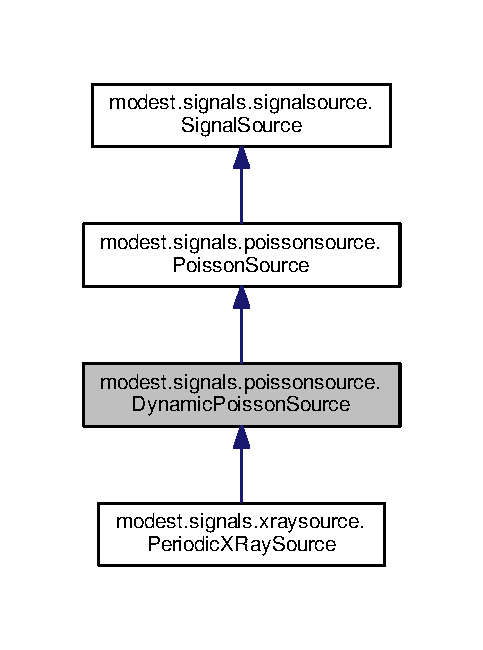
\includegraphics[width=232pt]{classmodest_1_1signals_1_1poissonsource_1_1DynamicPoissonSource__inherit__graph}
\end{center}
\end{figure}


Collaboration diagram for modest.\+signals.\+poissonsource.\+Dynamic\+Poisson\+Source\+:
\nopagebreak
\begin{figure}[H]
\begin{center}
\leavevmode
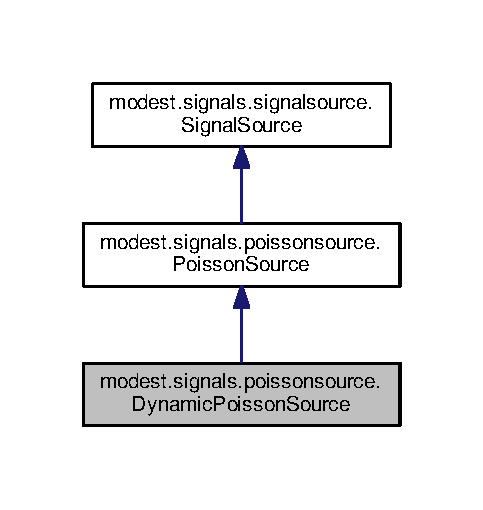
\includegraphics[width=232pt]{classmodest_1_1signals_1_1poissonsource_1_1DynamicPoissonSource__coll__graph}
\end{center}
\end{figure}
\subsection*{Public Member Functions}
\begin{DoxyCompactItemize}
\item 
def \hyperlink{classmodest_1_1signals_1_1poissonsource_1_1DynamicPoissonSource_a03a62ccbee75ae9feb563f63f046b20d}{\+\_\+\+\_\+init\+\_\+\+\_\+} (self, max\+Flux)
\item 
def \hyperlink{classmodest_1_1signals_1_1poissonsource_1_1DynamicPoissonSource_aa6030c607a4bded71c622f5f132c9bfe}{get\+Signal} (self, state, t, t\+Var=None)
\item 
def \hyperlink{classmodest_1_1signals_1_1poissonsource_1_1DynamicPoissonSource_a086252814ef8c2ddd3f4331dcfbbb827}{compute\+Association\+Probability} (self, measurement, state)
\item 
def \hyperlink{classmodest_1_1signals_1_1signalsource_1_1SignalSource_a3d32dbed840ea9ac775b226f0a654831}{compute\+Association\+Probability} (self, measurement, state\+Dict, validation\+Threshold=0)
\item 
def \hyperlink{classmodest_1_1signals_1_1signalsource_1_1SignalSource_a9a64c6a9c2954f6ad61e4ca3518ea8ab}{signal\+ID} (self)
\end{DoxyCompactItemize}
\subsection*{Public Attributes}
\begin{DoxyCompactItemize}
\item 
\hyperlink{classmodest_1_1signals_1_1poissonsource_1_1PoissonSource_a34395fc83bd8743a0a5ee69f9392a606}{last\+Time}
\item 
\hyperlink{classmodest_1_1signals_1_1poissonsource_1_1PoissonSource_a6f2c657ad936b921715d826ac74f7fe5}{flux}
\end{DoxyCompactItemize}
\subsection*{Static Public Attributes}
\begin{DoxyCompactItemize}
\item 
int \hyperlink{classmodest_1_1signals_1_1signalsource_1_1SignalSource_a453eafb550b551adbec0903deb63dfce}{next\+Signal\+ID} = 0
\end{DoxyCompactItemize}
\subsection*{Static Private Attributes}
\begin{DoxyCompactItemize}
\item 
\hyperlink{classmodest_1_1signals_1_1poissonsource_1_1DynamicPoissonSource_aa41498abaa3f69680ada7902aba5890f}{\+\_\+\+\_\+metaclass\+\_\+\+\_\+} = A\+B\+C\+Meta
\end{DoxyCompactItemize}


\subsection{Detailed Description}


Definition at line 46 of file poissonsource.\+py.



\subsection{Constructor \& Destructor Documentation}
\index{modest\+::signals\+::poissonsource\+::\+Dynamic\+Poisson\+Source@{modest\+::signals\+::poissonsource\+::\+Dynamic\+Poisson\+Source}!\+\_\+\+\_\+init\+\_\+\+\_\+@{\+\_\+\+\_\+init\+\_\+\+\_\+}}
\index{\+\_\+\+\_\+init\+\_\+\+\_\+@{\+\_\+\+\_\+init\+\_\+\+\_\+}!modest\+::signals\+::poissonsource\+::\+Dynamic\+Poisson\+Source@{modest\+::signals\+::poissonsource\+::\+Dynamic\+Poisson\+Source}}
\subsubsection[{\texorpdfstring{\+\_\+\+\_\+init\+\_\+\+\_\+(self, max\+Flux)}{__init__(self, maxFlux)}}]{\setlength{\rightskip}{0pt plus 5cm}def modest.\+signals.\+poissonsource.\+Dynamic\+Poisson\+Source.\+\_\+\+\_\+init\+\_\+\+\_\+ (
\begin{DoxyParamCaption}
\item[{}]{self, }
\item[{}]{max\+Flux}
\end{DoxyParamCaption}
)}\hypertarget{classmodest_1_1signals_1_1poissonsource_1_1DynamicPoissonSource_a03a62ccbee75ae9feb563f63f046b20d}{}\label{classmodest_1_1signals_1_1poissonsource_1_1DynamicPoissonSource_a03a62ccbee75ae9feb563f63f046b20d}


Definition at line 53 of file poissonsource.\+py.



\subsection{Member Function Documentation}
\index{modest\+::signals\+::poissonsource\+::\+Dynamic\+Poisson\+Source@{modest\+::signals\+::poissonsource\+::\+Dynamic\+Poisson\+Source}!compute\+Association\+Probability@{compute\+Association\+Probability}}
\index{compute\+Association\+Probability@{compute\+Association\+Probability}!modest\+::signals\+::poissonsource\+::\+Dynamic\+Poisson\+Source@{modest\+::signals\+::poissonsource\+::\+Dynamic\+Poisson\+Source}}
\subsubsection[{\texorpdfstring{compute\+Association\+Probability(self, measurement, state\+Dict, validation\+Threshold=0)}{computeAssociationProbability(self, measurement, stateDict, validationThreshold=0)}}]{\setlength{\rightskip}{0pt plus 5cm}def modest.\+signals.\+signalsource.\+Signal\+Source.\+compute\+Association\+Probability (
\begin{DoxyParamCaption}
\item[{}]{self, }
\item[{}]{measurement, }
\item[{}]{state\+Dict, }
\item[{}]{validation\+Threshold = {\ttfamily 0}}
\end{DoxyParamCaption}
)\hspace{0.3cm}{\ttfamily [inherited]}}\hypertarget{classmodest_1_1signals_1_1signalsource_1_1SignalSource_a3d32dbed840ea9ac775b226f0a654831}{}\label{classmodest_1_1signals_1_1signalsource_1_1SignalSource_a3d32dbed840ea9ac775b226f0a654831}


Definition at line 26 of file signalsource.\+py.

\index{modest\+::signals\+::poissonsource\+::\+Dynamic\+Poisson\+Source@{modest\+::signals\+::poissonsource\+::\+Dynamic\+Poisson\+Source}!compute\+Association\+Probability@{compute\+Association\+Probability}}
\index{compute\+Association\+Probability@{compute\+Association\+Probability}!modest\+::signals\+::poissonsource\+::\+Dynamic\+Poisson\+Source@{modest\+::signals\+::poissonsource\+::\+Dynamic\+Poisson\+Source}}
\subsubsection[{\texorpdfstring{compute\+Association\+Probability(self, measurement, state)}{computeAssociationProbability(self, measurement, state)}}]{\setlength{\rightskip}{0pt plus 5cm}def modest.\+signals.\+poissonsource.\+Dynamic\+Poisson\+Source.\+compute\+Association\+Probability (
\begin{DoxyParamCaption}
\item[{}]{self, }
\item[{}]{measurement, }
\item[{}]{state}
\end{DoxyParamCaption}
)}\hypertarget{classmodest_1_1signals_1_1poissonsource_1_1DynamicPoissonSource_a086252814ef8c2ddd3f4331dcfbbb827}{}\label{classmodest_1_1signals_1_1poissonsource_1_1DynamicPoissonSource_a086252814ef8c2ddd3f4331dcfbbb827}


Definition at line 73 of file poissonsource.\+py.

\index{modest\+::signals\+::poissonsource\+::\+Dynamic\+Poisson\+Source@{modest\+::signals\+::poissonsource\+::\+Dynamic\+Poisson\+Source}!get\+Signal@{get\+Signal}}
\index{get\+Signal@{get\+Signal}!modest\+::signals\+::poissonsource\+::\+Dynamic\+Poisson\+Source@{modest\+::signals\+::poissonsource\+::\+Dynamic\+Poisson\+Source}}
\subsubsection[{\texorpdfstring{get\+Signal(self, state, t, t\+Var=\+None)}{getSignal(self, state, t, tVar=None)}}]{\setlength{\rightskip}{0pt plus 5cm}def modest.\+signals.\+poissonsource.\+Dynamic\+Poisson\+Source.\+get\+Signal (
\begin{DoxyParamCaption}
\item[{}]{self, }
\item[{}]{state, }
\item[{}]{t, }
\item[{}]{t\+Var = {\ttfamily None}}
\end{DoxyParamCaption}
)}\hypertarget{classmodest_1_1signals_1_1poissonsource_1_1DynamicPoissonSource_aa6030c607a4bded71c622f5f132c9bfe}{}\label{classmodest_1_1signals_1_1poissonsource_1_1DynamicPoissonSource_aa6030c607a4bded71c622f5f132c9bfe}


Definition at line 63 of file poissonsource.\+py.

\index{modest\+::signals\+::poissonsource\+::\+Dynamic\+Poisson\+Source@{modest\+::signals\+::poissonsource\+::\+Dynamic\+Poisson\+Source}!signal\+ID@{signal\+ID}}
\index{signal\+ID@{signal\+ID}!modest\+::signals\+::poissonsource\+::\+Dynamic\+Poisson\+Source@{modest\+::signals\+::poissonsource\+::\+Dynamic\+Poisson\+Source}}
\subsubsection[{\texorpdfstring{signal\+I\+D(self)}{signalID(self)}}]{\setlength{\rightskip}{0pt plus 5cm}def modest.\+signals.\+signalsource.\+Signal\+Source.\+signal\+ID (
\begin{DoxyParamCaption}
\item[{}]{self}
\end{DoxyParamCaption}
)\hspace{0.3cm}{\ttfamily [inherited]}}\hypertarget{classmodest_1_1signals_1_1signalsource_1_1SignalSource_a9a64c6a9c2954f6ad61e4ca3518ea8ab}{}\label{classmodest_1_1signals_1_1signalsource_1_1SignalSource_a9a64c6a9c2954f6ad61e4ca3518ea8ab}


Definition at line 17 of file signalsource.\+py.



\subsection{Member Data Documentation}
\index{modest\+::signals\+::poissonsource\+::\+Dynamic\+Poisson\+Source@{modest\+::signals\+::poissonsource\+::\+Dynamic\+Poisson\+Source}!\+\_\+\+\_\+metaclass\+\_\+\+\_\+@{\+\_\+\+\_\+metaclass\+\_\+\+\_\+}}
\index{\+\_\+\+\_\+metaclass\+\_\+\+\_\+@{\+\_\+\+\_\+metaclass\+\_\+\+\_\+}!modest\+::signals\+::poissonsource\+::\+Dynamic\+Poisson\+Source@{modest\+::signals\+::poissonsource\+::\+Dynamic\+Poisson\+Source}}
\subsubsection[{\texorpdfstring{\+\_\+\+\_\+metaclass\+\_\+\+\_\+}{__metaclass__}}]{\setlength{\rightskip}{0pt plus 5cm}modest.\+signals.\+poissonsource.\+Dynamic\+Poisson\+Source.\+\_\+\+\_\+metaclass\+\_\+\+\_\+ = A\+B\+C\+Meta\hspace{0.3cm}{\ttfamily [static]}, {\ttfamily [private]}}\hypertarget{classmodest_1_1signals_1_1poissonsource_1_1DynamicPoissonSource_aa41498abaa3f69680ada7902aba5890f}{}\label{classmodest_1_1signals_1_1poissonsource_1_1DynamicPoissonSource_aa41498abaa3f69680ada7902aba5890f}


Definition at line 48 of file poissonsource.\+py.

\index{modest\+::signals\+::poissonsource\+::\+Dynamic\+Poisson\+Source@{modest\+::signals\+::poissonsource\+::\+Dynamic\+Poisson\+Source}!flux@{flux}}
\index{flux@{flux}!modest\+::signals\+::poissonsource\+::\+Dynamic\+Poisson\+Source@{modest\+::signals\+::poissonsource\+::\+Dynamic\+Poisson\+Source}}
\subsubsection[{\texorpdfstring{flux}{flux}}]{\setlength{\rightskip}{0pt plus 5cm}modest.\+signals.\+poissonsource.\+Poisson\+Source.\+flux\hspace{0.3cm}{\ttfamily [inherited]}}\hypertarget{classmodest_1_1signals_1_1poissonsource_1_1PoissonSource_a6f2c657ad936b921715d826ac74f7fe5}{}\label{classmodest_1_1signals_1_1poissonsource_1_1PoissonSource_a6f2c657ad936b921715d826ac74f7fe5}


Definition at line 14 of file poissonsource.\+py.

\index{modest\+::signals\+::poissonsource\+::\+Dynamic\+Poisson\+Source@{modest\+::signals\+::poissonsource\+::\+Dynamic\+Poisson\+Source}!last\+Time@{last\+Time}}
\index{last\+Time@{last\+Time}!modest\+::signals\+::poissonsource\+::\+Dynamic\+Poisson\+Source@{modest\+::signals\+::poissonsource\+::\+Dynamic\+Poisson\+Source}}
\subsubsection[{\texorpdfstring{last\+Time}{lastTime}}]{\setlength{\rightskip}{0pt plus 5cm}modest.\+signals.\+poissonsource.\+Poisson\+Source.\+last\+Time\hspace{0.3cm}{\ttfamily [inherited]}}\hypertarget{classmodest_1_1signals_1_1poissonsource_1_1PoissonSource_a34395fc83bd8743a0a5ee69f9392a606}{}\label{classmodest_1_1signals_1_1poissonsource_1_1PoissonSource_a34395fc83bd8743a0a5ee69f9392a606}


Definition at line 13 of file poissonsource.\+py.

\index{modest\+::signals\+::poissonsource\+::\+Dynamic\+Poisson\+Source@{modest\+::signals\+::poissonsource\+::\+Dynamic\+Poisson\+Source}!next\+Signal\+ID@{next\+Signal\+ID}}
\index{next\+Signal\+ID@{next\+Signal\+ID}!modest\+::signals\+::poissonsource\+::\+Dynamic\+Poisson\+Source@{modest\+::signals\+::poissonsource\+::\+Dynamic\+Poisson\+Source}}
\subsubsection[{\texorpdfstring{next\+Signal\+ID}{nextSignalID}}]{\setlength{\rightskip}{0pt plus 5cm}int modest.\+signals.\+signalsource.\+Signal\+Source.\+next\+Signal\+ID = 0\hspace{0.3cm}{\ttfamily [static]}, {\ttfamily [inherited]}}\hypertarget{classmodest_1_1signals_1_1signalsource_1_1SignalSource_a453eafb550b551adbec0903deb63dfce}{}\label{classmodest_1_1signals_1_1signalsource_1_1SignalSource_a453eafb550b551adbec0903deb63dfce}


Definition at line 8 of file signalsource.\+py.



The documentation for this class was generated from the following file\+:\begin{DoxyCompactItemize}
\item 
modest/signals/\hyperlink{poissonsource_8py}{poissonsource.\+py}\end{DoxyCompactItemize}

\hypertarget{classmodest_1_1modularfilter_1_1ModularFilter}{}\section{modest.\+modularfilter.\+Modular\+Filter Class Reference}
\label{classmodest_1_1modularfilter_1_1ModularFilter}\index{modest.\+modularfilter.\+Modular\+Filter@{modest.\+modularfilter.\+Modular\+Filter}}
\subsection*{Public Member Functions}
\begin{DoxyCompactItemize}
\item 
def \hyperlink{classmodest_1_1modularfilter_1_1ModularFilter_a20bc12664d580ca75518948229c10d13}{\+\_\+\+\_\+init\+\_\+\+\_\+} (self, \hyperlink{classmodest_1_1modularfilter_1_1ModularFilter_af91295c2d8f45afe04386215b5fa39aa}{measurement\+Validation\+Threshold}=1e-\/3, time=0, covariance\+Storage=\textquotesingle{}covariance\textquotesingle{})
\item 
def \hyperlink{classmodest_1_1modularfilter_1_1ModularFilter_a6363266b6fbd79b2cb8071c853af60a0}{add\+States} (self, name, state\+Object)
\item 
def \hyperlink{classmodest_1_1modularfilter_1_1ModularFilter_a6833080d980ec89769625721fa8e103d}{add\+Signal\+Source} (self, name, signal\+Source\+Object)
\item 
def \hyperlink{classmodest_1_1modularfilter_1_1ModularFilter_a7487bb7b6cad0d3af34c100d14e2e0a8}{time\+Update\+E\+KF} (self, dT, dynamics=None)
\item 
def \hyperlink{classmodest_1_1modularfilter_1_1ModularFilter_a39d5e1ab6cb950e4854eb909c338372c}{compute\+Association\+Probabilities} (self, measurement)
\item 
def \hyperlink{classmodest_1_1modularfilter_1_1ModularFilter_a493ccf6845ed800d565f1d26d063592c}{measurement\+Update\+E\+KF} (self, measurement, source\+Name)
\item 
def \hyperlink{classmodest_1_1modularfilter_1_1ModularFilter_af1a7d5a4e219c494de176f94997ae110}{measurement\+Update\+ML} (self, measurement)
\item 
def \hyperlink{classmodest_1_1modularfilter_1_1ModularFilter_ac3a26e2a7672ceedf00c48723104d55c}{measurement\+Update\+J\+P\+D\+AF} (self, measurement)
\item 
def \hyperlink{classmodest_1_1modularfilter_1_1ModularFilter_a11fd7a3b3bcd145f32190f53462c974a}{get\+Global\+State\+Vector} (self)
\item 
def \hyperlink{classmodest_1_1modularfilter_1_1ModularFilter_a15412a15695827fc57a0609000a1c9c0}{store\+Global\+State\+Vector} (self, global\+State\+Vector, covariance, a\+Priori=False)
\item 
def \hyperlink{classmodest_1_1modularfilter_1_1ModularFilter_ab1dc914f4939e1219f4f2d0efbafd9dd}{local\+State\+Update\+Matrices} (self, measurement, signal\+Source\+Name, x\+Minus, P\+Minus)
\item 
def \hyperlink{classmodest_1_1modularfilter_1_1ModularFilter_ada608a31a2fb8bee8965042c134ead47}{compute\+Updated\+Stateand\+Covariance} (self, x\+Minus, P\+Minus, dY, H, R)
\item 
def \hyperlink{classmodest_1_1modularfilter_1_1ModularFilter_aafbb97419cd23cddddf96d61e577b584}{initialize\+Real\+Time\+Plot} (self, \hyperlink{classmodest_1_1modularfilter_1_1ModularFilter_a2945291a2115aba2680a7c1a1cf728fc}{plot\+Handle}=None)
\item 
def \hyperlink{classmodest_1_1modularfilter_1_1ModularFilter_a028d2750278a922bb89e895b53112452}{real\+Time\+Plot} (self, normalized=True)
\end{DoxyCompactItemize}
\subsection*{Static Public Member Functions}
\begin{DoxyCompactItemize}
\item 
def \hyperlink{classmodest_1_1modularfilter_1_1ModularFilter_a23cedf0034dc1878c7c7ff2d970640d8}{covariance\+Inverse} (P)
\end{DoxyCompactItemize}
\subsection*{Public Attributes}
\begin{DoxyCompactItemize}
\item 
\hyperlink{classmodest_1_1modularfilter_1_1ModularFilter_a96114547940eb463174477fe4612c999}{covariance\+Storage}
\begin{DoxyCompactList}\small\item\em covariance\+Storage determines how the filter stores and updates covariance, or more generally, uncertainty. \end{DoxyCompactList}\item 
\hyperlink{classmodest_1_1modularfilter_1_1ModularFilter_a2945291a2115aba2680a7c1a1cf728fc}{plot\+Handle}
\item 
\hyperlink{classmodest_1_1modularfilter_1_1ModularFilter_ae7028964e7e7adf58d75b76aef9783f6}{total\+Dimension}
\item 
\hyperlink{classmodest_1_1modularfilter_1_1ModularFilter_ac1b2e8a44ee25a8a2935e6e44a8409e5}{covariance\+Matrix}
\item 
\hyperlink{classmodest_1_1modularfilter_1_1ModularFilter_a80c66c525d5afd61271f13da47148c5d}{sub\+States}
\item 
\hyperlink{classmodest_1_1modularfilter_1_1ModularFilter_a545ac50ec6f67f29ad3420cfc5581812}{signal\+Sources}
\item 
\hyperlink{classmodest_1_1modularfilter_1_1ModularFilter_a917f511b39632b804f3ecf667f5a6d96}{t\+Current}
\item 
\hyperlink{classmodest_1_1modularfilter_1_1ModularFilter_af91295c2d8f45afe04386215b5fa39aa}{measurement\+Validation\+Threshold}
\item 
\hyperlink{classmodest_1_1modularfilter_1_1ModularFilter_a691b2974939eedf436beea187b0714dd}{measurement\+List}
\item 
\hyperlink{classmodest_1_1modularfilter_1_1ModularFilter_adc22328f3634e2b7bdeff883a7398538}{last\+Measurement\+ID}
\item 
\hyperlink{classmodest_1_1modularfilter_1_1ModularFilter_ab68eefa9ffabb7f9b4b4622fd7686fa0}{last\+State\+Vector\+ID}
\end{DoxyCompactItemize}


\subsection{Detailed Description}
This class is designed to facilitate a variety of estimation algorithms in a modular way, i.\+e. in a way that allows maximum amount of flexibility with minimum amount of code duplication.

The idea behind this class is that all of the functions which are \char`\"{}generic\char`\"{} to an estimation algorithm can be written just once, as a part of this class. Then the code contained here can be implemented on a variety of different estimation problems without having to duplicate code.

The basic estimation model implemented here works as follows. The overall state, i.\+e. all of the quantities to be estimated, are represented by Sub\+States.\+Sub\+State objects. Measurements of these states are represented by Signals.\+Signal\+Source objects. The \hyperlink{classmodest_1_1modularfilter_1_1ModularFilter}{Modular\+Filter} class is responsible for doing time-\/updates and measurement-\/updates on these states. These objects are responsible for doing all of the things that are particular to those states, and those signals, respectively. For instance, generation of time-\/update and measurement update matrices is handled by the Sub\+States.\+Sub\+State objects. 

Definition at line 48 of file modularfilter.\+py.



\subsection{Constructor \& Destructor Documentation}
\index{modest\+::modularfilter\+::\+Modular\+Filter@{modest\+::modularfilter\+::\+Modular\+Filter}!\+\_\+\+\_\+init\+\_\+\+\_\+@{\+\_\+\+\_\+init\+\_\+\+\_\+}}
\index{\+\_\+\+\_\+init\+\_\+\+\_\+@{\+\_\+\+\_\+init\+\_\+\+\_\+}!modest\+::modularfilter\+::\+Modular\+Filter@{modest\+::modularfilter\+::\+Modular\+Filter}}
\subsubsection[{\texorpdfstring{\+\_\+\+\_\+init\+\_\+\+\_\+(self, measurement\+Validation\+Threshold=1e-\/3, time=0, covariance\+Storage=\textquotesingle{}covariance\textquotesingle{})}{__init__(self, measurementValidationThreshold=1e-3, time=0, covarianceStorage='covariance')}}]{\setlength{\rightskip}{0pt plus 5cm}def modest.\+modularfilter.\+Modular\+Filter.\+\_\+\+\_\+init\+\_\+\+\_\+ (
\begin{DoxyParamCaption}
\item[{}]{self, }
\item[{}]{measurement\+Validation\+Threshold = {\ttfamily 1e-\/3}, }
\item[{}]{time = {\ttfamily 0}, }
\item[{}]{covariance\+Storage = {\ttfamily \textquotesingle{}covariance\textquotesingle{}}}
\end{DoxyParamCaption}
)}\hypertarget{classmodest_1_1modularfilter_1_1ModularFilter_a20bc12664d580ca75518948229c10d13}{}\label{classmodest_1_1modularfilter_1_1ModularFilter_a20bc12664d580ca75518948229c10d13}


Definition at line 54 of file modularfilter.\+py.



\subsection{Member Function Documentation}
\index{modest\+::modularfilter\+::\+Modular\+Filter@{modest\+::modularfilter\+::\+Modular\+Filter}!add\+Signal\+Source@{add\+Signal\+Source}}
\index{add\+Signal\+Source@{add\+Signal\+Source}!modest\+::modularfilter\+::\+Modular\+Filter@{modest\+::modularfilter\+::\+Modular\+Filter}}
\subsubsection[{\texorpdfstring{add\+Signal\+Source(self, name, signal\+Source\+Object)}{addSignalSource(self, name, signalSourceObject)}}]{\setlength{\rightskip}{0pt plus 5cm}def modest.\+modularfilter.\+Modular\+Filter.\+add\+Signal\+Source (
\begin{DoxyParamCaption}
\item[{}]{self, }
\item[{}]{name, }
\item[{}]{signal\+Source\+Object}
\end{DoxyParamCaption}
)}\hypertarget{classmodest_1_1modularfilter_1_1ModularFilter_a6833080d980ec89769625721fa8e103d}{}\label{classmodest_1_1modularfilter_1_1ModularFilter_a6833080d980ec89769625721fa8e103d}


Definition at line 140 of file modularfilter.\+py.

\index{modest\+::modularfilter\+::\+Modular\+Filter@{modest\+::modularfilter\+::\+Modular\+Filter}!add\+States@{add\+States}}
\index{add\+States@{add\+States}!modest\+::modularfilter\+::\+Modular\+Filter@{modest\+::modularfilter\+::\+Modular\+Filter}}
\subsubsection[{\texorpdfstring{add\+States(self, name, state\+Object)}{addStates(self, name, stateObject)}}]{\setlength{\rightskip}{0pt plus 5cm}def modest.\+modularfilter.\+Modular\+Filter.\+add\+States (
\begin{DoxyParamCaption}
\item[{}]{self, }
\item[{}]{name, }
\item[{}]{state\+Object}
\end{DoxyParamCaption}
)}\hypertarget{classmodest_1_1modularfilter_1_1ModularFilter_a6363266b6fbd79b2cb8071c853af60a0}{}\label{classmodest_1_1modularfilter_1_1ModularFilter_a6363266b6fbd79b2cb8071c853af60a0}


Definition at line 90 of file modularfilter.\+py.

\index{modest\+::modularfilter\+::\+Modular\+Filter@{modest\+::modularfilter\+::\+Modular\+Filter}!compute\+Association\+Probabilities@{compute\+Association\+Probabilities}}
\index{compute\+Association\+Probabilities@{compute\+Association\+Probabilities}!modest\+::modularfilter\+::\+Modular\+Filter@{modest\+::modularfilter\+::\+Modular\+Filter}}
\subsubsection[{\texorpdfstring{compute\+Association\+Probabilities(self, measurement)}{computeAssociationProbabilities(self, measurement)}}]{\setlength{\rightskip}{0pt plus 5cm}def modest.\+modularfilter.\+Modular\+Filter.\+compute\+Association\+Probabilities (
\begin{DoxyParamCaption}
\item[{}]{self, }
\item[{}]{measurement}
\end{DoxyParamCaption}
)}\hypertarget{classmodest_1_1modularfilter_1_1ModularFilter_a39d5e1ab6cb950e4854eb909c338372c}{}\label{classmodest_1_1modularfilter_1_1ModularFilter_a39d5e1ab6cb950e4854eb909c338372c}


Definition at line 243 of file modularfilter.\+py.

\index{modest\+::modularfilter\+::\+Modular\+Filter@{modest\+::modularfilter\+::\+Modular\+Filter}!compute\+Updated\+Stateand\+Covariance@{compute\+Updated\+Stateand\+Covariance}}
\index{compute\+Updated\+Stateand\+Covariance@{compute\+Updated\+Stateand\+Covariance}!modest\+::modularfilter\+::\+Modular\+Filter@{modest\+::modularfilter\+::\+Modular\+Filter}}
\subsubsection[{\texorpdfstring{compute\+Updated\+Stateand\+Covariance(self, x\+Minus, P\+Minus, d\+Y, H, R)}{computeUpdatedStateandCovariance(self, xMinus, PMinus, dY, H, R)}}]{\setlength{\rightskip}{0pt plus 5cm}def modest.\+modularfilter.\+Modular\+Filter.\+compute\+Updated\+Stateand\+Covariance (
\begin{DoxyParamCaption}
\item[{}]{self, }
\item[{}]{x\+Minus, }
\item[{}]{P\+Minus, }
\item[{}]{dY, }
\item[{}]{H, }
\item[{}]{R}
\end{DoxyParamCaption}
)}\hypertarget{classmodest_1_1modularfilter_1_1ModularFilter_ada608a31a2fb8bee8965042c134ead47}{}\label{classmodest_1_1modularfilter_1_1ModularFilter_ada608a31a2fb8bee8965042c134ead47}


Definition at line 798 of file modularfilter.\+py.

\index{modest\+::modularfilter\+::\+Modular\+Filter@{modest\+::modularfilter\+::\+Modular\+Filter}!covariance\+Inverse@{covariance\+Inverse}}
\index{covariance\+Inverse@{covariance\+Inverse}!modest\+::modularfilter\+::\+Modular\+Filter@{modest\+::modularfilter\+::\+Modular\+Filter}}
\subsubsection[{\texorpdfstring{covariance\+Inverse(\+P)}{covarianceInverse(P)}}]{\setlength{\rightskip}{0pt plus 5cm}def modest.\+modularfilter.\+Modular\+Filter.\+covariance\+Inverse (
\begin{DoxyParamCaption}
\item[{}]{P}
\end{DoxyParamCaption}
)\hspace{0.3cm}{\ttfamily [static]}}\hypertarget{classmodest_1_1modularfilter_1_1ModularFilter_a23cedf0034dc1878c7c7ff2d970640d8}{}\label{classmodest_1_1modularfilter_1_1ModularFilter_a23cedf0034dc1878c7c7ff2d970640d8}


Definition at line 846 of file modularfilter.\+py.

\index{modest\+::modularfilter\+::\+Modular\+Filter@{modest\+::modularfilter\+::\+Modular\+Filter}!get\+Global\+State\+Vector@{get\+Global\+State\+Vector}}
\index{get\+Global\+State\+Vector@{get\+Global\+State\+Vector}!modest\+::modularfilter\+::\+Modular\+Filter@{modest\+::modularfilter\+::\+Modular\+Filter}}
\subsubsection[{\texorpdfstring{get\+Global\+State\+Vector(self)}{getGlobalStateVector(self)}}]{\setlength{\rightskip}{0pt plus 5cm}def modest.\+modularfilter.\+Modular\+Filter.\+get\+Global\+State\+Vector (
\begin{DoxyParamCaption}
\item[{}]{self}
\end{DoxyParamCaption}
)}\hypertarget{classmodest_1_1modularfilter_1_1ModularFilter_a11fd7a3b3bcd145f32190f53462c974a}{}\label{classmodest_1_1modularfilter_1_1ModularFilter_a11fd7a3b3bcd145f32190f53462c974a}


Definition at line 549 of file modularfilter.\+py.

\index{modest\+::modularfilter\+::\+Modular\+Filter@{modest\+::modularfilter\+::\+Modular\+Filter}!initialize\+Real\+Time\+Plot@{initialize\+Real\+Time\+Plot}}
\index{initialize\+Real\+Time\+Plot@{initialize\+Real\+Time\+Plot}!modest\+::modularfilter\+::\+Modular\+Filter@{modest\+::modularfilter\+::\+Modular\+Filter}}
\subsubsection[{\texorpdfstring{initialize\+Real\+Time\+Plot(self, plot\+Handle=\+None)}{initializeRealTimePlot(self, plotHandle=None)}}]{\setlength{\rightskip}{0pt plus 5cm}def modest.\+modularfilter.\+Modular\+Filter.\+initialize\+Real\+Time\+Plot (
\begin{DoxyParamCaption}
\item[{}]{self, }
\item[{}]{plot\+Handle = {\ttfamily None}}
\end{DoxyParamCaption}
)}\hypertarget{classmodest_1_1modularfilter_1_1ModularFilter_aafbb97419cd23cddddf96d61e577b584}{}\label{classmodest_1_1modularfilter_1_1ModularFilter_aafbb97419cd23cddddf96d61e577b584}


Definition at line 853 of file modularfilter.\+py.

\index{modest\+::modularfilter\+::\+Modular\+Filter@{modest\+::modularfilter\+::\+Modular\+Filter}!local\+State\+Update\+Matrices@{local\+State\+Update\+Matrices}}
\index{local\+State\+Update\+Matrices@{local\+State\+Update\+Matrices}!modest\+::modularfilter\+::\+Modular\+Filter@{modest\+::modularfilter\+::\+Modular\+Filter}}
\subsubsection[{\texorpdfstring{local\+State\+Update\+Matrices(self, measurement, signal\+Source\+Name, x\+Minus, P\+Minus)}{localStateUpdateMatrices(self, measurement, signalSourceName, xMinus, PMinus)}}]{\setlength{\rightskip}{0pt plus 5cm}def modest.\+modularfilter.\+Modular\+Filter.\+local\+State\+Update\+Matrices (
\begin{DoxyParamCaption}
\item[{}]{self, }
\item[{}]{measurement, }
\item[{}]{signal\+Source\+Name, }
\item[{}]{x\+Minus, }
\item[{}]{P\+Minus}
\end{DoxyParamCaption}
)}\hypertarget{classmodest_1_1modularfilter_1_1ModularFilter_ab1dc914f4939e1219f4f2d0efbafd9dd}{}\label{classmodest_1_1modularfilter_1_1ModularFilter_ab1dc914f4939e1219f4f2d0efbafd9dd}


Definition at line 601 of file modularfilter.\+py.

\index{modest\+::modularfilter\+::\+Modular\+Filter@{modest\+::modularfilter\+::\+Modular\+Filter}!measurement\+Update\+E\+KF@{measurement\+Update\+E\+KF}}
\index{measurement\+Update\+E\+KF@{measurement\+Update\+E\+KF}!modest\+::modularfilter\+::\+Modular\+Filter@{modest\+::modularfilter\+::\+Modular\+Filter}}
\subsubsection[{\texorpdfstring{measurement\+Update\+E\+K\+F(self, measurement, source\+Name)}{measurementUpdateEKF(self, measurement, sourceName)}}]{\setlength{\rightskip}{0pt plus 5cm}def modest.\+modularfilter.\+Modular\+Filter.\+measurement\+Update\+E\+KF (
\begin{DoxyParamCaption}
\item[{}]{self, }
\item[{}]{measurement, }
\item[{}]{source\+Name}
\end{DoxyParamCaption}
)}\hypertarget{classmodest_1_1modularfilter_1_1ModularFilter_a493ccf6845ed800d565f1d26d063592c}{}\label{classmodest_1_1modularfilter_1_1ModularFilter_a493ccf6845ed800d565f1d26d063592c}


Definition at line 299 of file modularfilter.\+py.

\index{modest\+::modularfilter\+::\+Modular\+Filter@{modest\+::modularfilter\+::\+Modular\+Filter}!measurement\+Update\+J\+P\+D\+AF@{measurement\+Update\+J\+P\+D\+AF}}
\index{measurement\+Update\+J\+P\+D\+AF@{measurement\+Update\+J\+P\+D\+AF}!modest\+::modularfilter\+::\+Modular\+Filter@{modest\+::modularfilter\+::\+Modular\+Filter}}
\subsubsection[{\texorpdfstring{measurement\+Update\+J\+P\+D\+A\+F(self, measurement)}{measurementUpdateJPDAF(self, measurement)}}]{\setlength{\rightskip}{0pt plus 5cm}def modest.\+modularfilter.\+Modular\+Filter.\+measurement\+Update\+J\+P\+D\+AF (
\begin{DoxyParamCaption}
\item[{}]{self, }
\item[{}]{measurement}
\end{DoxyParamCaption}
)}\hypertarget{classmodest_1_1modularfilter_1_1ModularFilter_ac3a26e2a7672ceedf00c48723104d55c}{}\label{classmodest_1_1modularfilter_1_1ModularFilter_ac3a26e2a7672ceedf00c48723104d55c}


Definition at line 377 of file modularfilter.\+py.

\index{modest\+::modularfilter\+::\+Modular\+Filter@{modest\+::modularfilter\+::\+Modular\+Filter}!measurement\+Update\+ML@{measurement\+Update\+ML}}
\index{measurement\+Update\+ML@{measurement\+Update\+ML}!modest\+::modularfilter\+::\+Modular\+Filter@{modest\+::modularfilter\+::\+Modular\+Filter}}
\subsubsection[{\texorpdfstring{measurement\+Update\+M\+L(self, measurement)}{measurementUpdateML(self, measurement)}}]{\setlength{\rightskip}{0pt plus 5cm}def modest.\+modularfilter.\+Modular\+Filter.\+measurement\+Update\+ML (
\begin{DoxyParamCaption}
\item[{}]{self, }
\item[{}]{measurement}
\end{DoxyParamCaption}
)}\hypertarget{classmodest_1_1modularfilter_1_1ModularFilter_af1a7d5a4e219c494de176f94997ae110}{}\label{classmodest_1_1modularfilter_1_1ModularFilter_af1a7d5a4e219c494de176f94997ae110}


Definition at line 335 of file modularfilter.\+py.

\index{modest\+::modularfilter\+::\+Modular\+Filter@{modest\+::modularfilter\+::\+Modular\+Filter}!real\+Time\+Plot@{real\+Time\+Plot}}
\index{real\+Time\+Plot@{real\+Time\+Plot}!modest\+::modularfilter\+::\+Modular\+Filter@{modest\+::modularfilter\+::\+Modular\+Filter}}
\subsubsection[{\texorpdfstring{real\+Time\+Plot(self, normalized=\+True)}{realTimePlot(self, normalized=True)}}]{\setlength{\rightskip}{0pt plus 5cm}def modest.\+modularfilter.\+Modular\+Filter.\+real\+Time\+Plot (
\begin{DoxyParamCaption}
\item[{}]{self, }
\item[{}]{normalized = {\ttfamily True}}
\end{DoxyParamCaption}
)}\hypertarget{classmodest_1_1modularfilter_1_1ModularFilter_a028d2750278a922bb89e895b53112452}{}\label{classmodest_1_1modularfilter_1_1ModularFilter_a028d2750278a922bb89e895b53112452}


Definition at line 875 of file modularfilter.\+py.

\index{modest\+::modularfilter\+::\+Modular\+Filter@{modest\+::modularfilter\+::\+Modular\+Filter}!store\+Global\+State\+Vector@{store\+Global\+State\+Vector}}
\index{store\+Global\+State\+Vector@{store\+Global\+State\+Vector}!modest\+::modularfilter\+::\+Modular\+Filter@{modest\+::modularfilter\+::\+Modular\+Filter}}
\subsubsection[{\texorpdfstring{store\+Global\+State\+Vector(self, global\+State\+Vector, covariance, a\+Priori=\+False)}{storeGlobalStateVector(self, globalStateVector, covariance, aPriori=False)}}]{\setlength{\rightskip}{0pt plus 5cm}def modest.\+modularfilter.\+Modular\+Filter.\+store\+Global\+State\+Vector (
\begin{DoxyParamCaption}
\item[{}]{self, }
\item[{}]{global\+State\+Vector, }
\item[{}]{covariance, }
\item[{}]{a\+Priori = {\ttfamily False}}
\end{DoxyParamCaption}
)}\hypertarget{classmodest_1_1modularfilter_1_1ModularFilter_a15412a15695827fc57a0609000a1c9c0}{}\label{classmodest_1_1modularfilter_1_1ModularFilter_a15412a15695827fc57a0609000a1c9c0}


Definition at line 563 of file modularfilter.\+py.

\index{modest\+::modularfilter\+::\+Modular\+Filter@{modest\+::modularfilter\+::\+Modular\+Filter}!time\+Update\+E\+KF@{time\+Update\+E\+KF}}
\index{time\+Update\+E\+KF@{time\+Update\+E\+KF}!modest\+::modularfilter\+::\+Modular\+Filter@{modest\+::modularfilter\+::\+Modular\+Filter}}
\subsubsection[{\texorpdfstring{time\+Update\+E\+K\+F(self, d\+T, dynamics=\+None)}{timeUpdateEKF(self, dT, dynamics=None)}}]{\setlength{\rightskip}{0pt plus 5cm}def modest.\+modularfilter.\+Modular\+Filter.\+time\+Update\+E\+KF (
\begin{DoxyParamCaption}
\item[{}]{self, }
\item[{}]{dT, }
\item[{}]{dynamics = {\ttfamily None}}
\end{DoxyParamCaption}
)}\hypertarget{classmodest_1_1modularfilter_1_1ModularFilter_a7487bb7b6cad0d3af34c100d14e2e0a8}{}\label{classmodest_1_1modularfilter_1_1ModularFilter_a7487bb7b6cad0d3af34c100d14e2e0a8}


Definition at line 159 of file modularfilter.\+py.



\subsection{Member Data Documentation}
\index{modest\+::modularfilter\+::\+Modular\+Filter@{modest\+::modularfilter\+::\+Modular\+Filter}!covariance\+Matrix@{covariance\+Matrix}}
\index{covariance\+Matrix@{covariance\+Matrix}!modest\+::modularfilter\+::\+Modular\+Filter@{modest\+::modularfilter\+::\+Modular\+Filter}}
\subsubsection[{\texorpdfstring{covariance\+Matrix}{covarianceMatrix}}]{\setlength{\rightskip}{0pt plus 5cm}modest.\+modularfilter.\+Modular\+Filter.\+covariance\+Matrix}\hypertarget{classmodest_1_1modularfilter_1_1ModularFilter_ac1b2e8a44ee25a8a2935e6e44a8409e5}{}\label{classmodest_1_1modularfilter_1_1ModularFilter_ac1b2e8a44ee25a8a2935e6e44a8409e5}


Definition at line 63 of file modularfilter.\+py.

\index{modest\+::modularfilter\+::\+Modular\+Filter@{modest\+::modularfilter\+::\+Modular\+Filter}!covariance\+Storage@{covariance\+Storage}}
\index{covariance\+Storage@{covariance\+Storage}!modest\+::modularfilter\+::\+Modular\+Filter@{modest\+::modularfilter\+::\+Modular\+Filter}}
\subsubsection[{\texorpdfstring{covariance\+Storage}{covarianceStorage}}]{\setlength{\rightskip}{0pt plus 5cm}modest.\+modularfilter.\+Modular\+Filter.\+covariance\+Storage}\hypertarget{classmodest_1_1modularfilter_1_1ModularFilter_a96114547940eb463174477fe4612c999}{}\label{classmodest_1_1modularfilter_1_1ModularFilter_a96114547940eb463174477fe4612c999}


covariance\+Storage determines how the filter stores and updates covariance, or more generally, uncertainty. 

The standard approach is to use the covariance matrix, as in the standard Kalman filter formulation. 

Definition at line 59 of file modularfilter.\+py.

\index{modest\+::modularfilter\+::\+Modular\+Filter@{modest\+::modularfilter\+::\+Modular\+Filter}!last\+Measurement\+ID@{last\+Measurement\+ID}}
\index{last\+Measurement\+ID@{last\+Measurement\+ID}!modest\+::modularfilter\+::\+Modular\+Filter@{modest\+::modularfilter\+::\+Modular\+Filter}}
\subsubsection[{\texorpdfstring{last\+Measurement\+ID}{lastMeasurementID}}]{\setlength{\rightskip}{0pt plus 5cm}modest.\+modularfilter.\+Modular\+Filter.\+last\+Measurement\+ID}\hypertarget{classmodest_1_1modularfilter_1_1ModularFilter_adc22328f3634e2b7bdeff883a7398538}{}\label{classmodest_1_1modularfilter_1_1ModularFilter_adc22328f3634e2b7bdeff883a7398538}


Definition at line 72 of file modularfilter.\+py.

\index{modest\+::modularfilter\+::\+Modular\+Filter@{modest\+::modularfilter\+::\+Modular\+Filter}!last\+State\+Vector\+ID@{last\+State\+Vector\+ID}}
\index{last\+State\+Vector\+ID@{last\+State\+Vector\+ID}!modest\+::modularfilter\+::\+Modular\+Filter@{modest\+::modularfilter\+::\+Modular\+Filter}}
\subsubsection[{\texorpdfstring{last\+State\+Vector\+ID}{lastStateVectorID}}]{\setlength{\rightskip}{0pt plus 5cm}modest.\+modularfilter.\+Modular\+Filter.\+last\+State\+Vector\+ID}\hypertarget{classmodest_1_1modularfilter_1_1ModularFilter_ab68eefa9ffabb7f9b4b4622fd7686fa0}{}\label{classmodest_1_1modularfilter_1_1ModularFilter_ab68eefa9ffabb7f9b4b4622fd7686fa0}


Definition at line 74 of file modularfilter.\+py.

\index{modest\+::modularfilter\+::\+Modular\+Filter@{modest\+::modularfilter\+::\+Modular\+Filter}!measurement\+List@{measurement\+List}}
\index{measurement\+List@{measurement\+List}!modest\+::modularfilter\+::\+Modular\+Filter@{modest\+::modularfilter\+::\+Modular\+Filter}}
\subsubsection[{\texorpdfstring{measurement\+List}{measurementList}}]{\setlength{\rightskip}{0pt plus 5cm}modest.\+modularfilter.\+Modular\+Filter.\+measurement\+List}\hypertarget{classmodest_1_1modularfilter_1_1ModularFilter_a691b2974939eedf436beea187b0714dd}{}\label{classmodest_1_1modularfilter_1_1ModularFilter_a691b2974939eedf436beea187b0714dd}


Definition at line 71 of file modularfilter.\+py.

\index{modest\+::modularfilter\+::\+Modular\+Filter@{modest\+::modularfilter\+::\+Modular\+Filter}!measurement\+Validation\+Threshold@{measurement\+Validation\+Threshold}}
\index{measurement\+Validation\+Threshold@{measurement\+Validation\+Threshold}!modest\+::modularfilter\+::\+Modular\+Filter@{modest\+::modularfilter\+::\+Modular\+Filter}}
\subsubsection[{\texorpdfstring{measurement\+Validation\+Threshold}{measurementValidationThreshold}}]{\setlength{\rightskip}{0pt plus 5cm}modest.\+modularfilter.\+Modular\+Filter.\+measurement\+Validation\+Threshold}\hypertarget{classmodest_1_1modularfilter_1_1ModularFilter_af91295c2d8f45afe04386215b5fa39aa}{}\label{classmodest_1_1modularfilter_1_1ModularFilter_af91295c2d8f45afe04386215b5fa39aa}


Definition at line 69 of file modularfilter.\+py.

\index{modest\+::modularfilter\+::\+Modular\+Filter@{modest\+::modularfilter\+::\+Modular\+Filter}!plot\+Handle@{plot\+Handle}}
\index{plot\+Handle@{plot\+Handle}!modest\+::modularfilter\+::\+Modular\+Filter@{modest\+::modularfilter\+::\+Modular\+Filter}}
\subsubsection[{\texorpdfstring{plot\+Handle}{plotHandle}}]{\setlength{\rightskip}{0pt plus 5cm}modest.\+modularfilter.\+Modular\+Filter.\+plot\+Handle}\hypertarget{classmodest_1_1modularfilter_1_1ModularFilter_a2945291a2115aba2680a7c1a1cf728fc}{}\label{classmodest_1_1modularfilter_1_1ModularFilter_a2945291a2115aba2680a7c1a1cf728fc}


Definition at line 60 of file modularfilter.\+py.

\index{modest\+::modularfilter\+::\+Modular\+Filter@{modest\+::modularfilter\+::\+Modular\+Filter}!signal\+Sources@{signal\+Sources}}
\index{signal\+Sources@{signal\+Sources}!modest\+::modularfilter\+::\+Modular\+Filter@{modest\+::modularfilter\+::\+Modular\+Filter}}
\subsubsection[{\texorpdfstring{signal\+Sources}{signalSources}}]{\setlength{\rightskip}{0pt plus 5cm}modest.\+modularfilter.\+Modular\+Filter.\+signal\+Sources}\hypertarget{classmodest_1_1modularfilter_1_1ModularFilter_a545ac50ec6f67f29ad3420cfc5581812}{}\label{classmodest_1_1modularfilter_1_1ModularFilter_a545ac50ec6f67f29ad3420cfc5581812}


Definition at line 66 of file modularfilter.\+py.

\index{modest\+::modularfilter\+::\+Modular\+Filter@{modest\+::modularfilter\+::\+Modular\+Filter}!sub\+States@{sub\+States}}
\index{sub\+States@{sub\+States}!modest\+::modularfilter\+::\+Modular\+Filter@{modest\+::modularfilter\+::\+Modular\+Filter}}
\subsubsection[{\texorpdfstring{sub\+States}{subStates}}]{\setlength{\rightskip}{0pt plus 5cm}modest.\+modularfilter.\+Modular\+Filter.\+sub\+States}\hypertarget{classmodest_1_1modularfilter_1_1ModularFilter_a80c66c525d5afd61271f13da47148c5d}{}\label{classmodest_1_1modularfilter_1_1ModularFilter_a80c66c525d5afd61271f13da47148c5d}


Definition at line 65 of file modularfilter.\+py.

\index{modest\+::modularfilter\+::\+Modular\+Filter@{modest\+::modularfilter\+::\+Modular\+Filter}!t\+Current@{t\+Current}}
\index{t\+Current@{t\+Current}!modest\+::modularfilter\+::\+Modular\+Filter@{modest\+::modularfilter\+::\+Modular\+Filter}}
\subsubsection[{\texorpdfstring{t\+Current}{tCurrent}}]{\setlength{\rightskip}{0pt plus 5cm}modest.\+modularfilter.\+Modular\+Filter.\+t\+Current}\hypertarget{classmodest_1_1modularfilter_1_1ModularFilter_a917f511b39632b804f3ecf667f5a6d96}{}\label{classmodest_1_1modularfilter_1_1ModularFilter_a917f511b39632b804f3ecf667f5a6d96}


Definition at line 67 of file modularfilter.\+py.

\index{modest\+::modularfilter\+::\+Modular\+Filter@{modest\+::modularfilter\+::\+Modular\+Filter}!total\+Dimension@{total\+Dimension}}
\index{total\+Dimension@{total\+Dimension}!modest\+::modularfilter\+::\+Modular\+Filter@{modest\+::modularfilter\+::\+Modular\+Filter}}
\subsubsection[{\texorpdfstring{total\+Dimension}{totalDimension}}]{\setlength{\rightskip}{0pt plus 5cm}modest.\+modularfilter.\+Modular\+Filter.\+total\+Dimension}\hypertarget{classmodest_1_1modularfilter_1_1ModularFilter_ae7028964e7e7adf58d75b76aef9783f6}{}\label{classmodest_1_1modularfilter_1_1ModularFilter_ae7028964e7e7adf58d75b76aef9783f6}


Definition at line 62 of file modularfilter.\+py.



The documentation for this class was generated from the following file\+:\begin{DoxyCompactItemize}
\item 
modest/\hyperlink{modularfilter_8py}{modularfilter.\+py}\end{DoxyCompactItemize}

\hypertarget{classmodest_1_1signals_1_1oneDimensionalObject_1_1oneDObjectMeasurement}{}\section{modest.\+signals.\+one\+Dimensional\+Object.\+one\+D\+Object\+Measurement Class Reference}
\label{classmodest_1_1signals_1_1oneDimensionalObject_1_1oneDObjectMeasurement}\index{modest.\+signals.\+one\+Dimensional\+Object.\+one\+D\+Object\+Measurement@{modest.\+signals.\+one\+Dimensional\+Object.\+one\+D\+Object\+Measurement}}


Inheritance diagram for modest.\+signals.\+one\+Dimensional\+Object.\+one\+D\+Object\+Measurement\+:
\nopagebreak
\begin{figure}[H]
\begin{center}
\leavevmode
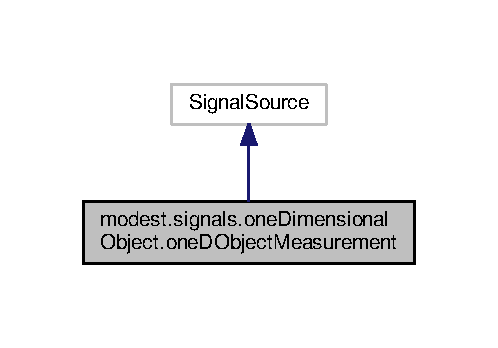
\includegraphics[width=239pt]{classmodest_1_1signals_1_1oneDimensionalObject_1_1oneDObjectMeasurement__inherit__graph}
\end{center}
\end{figure}


Collaboration diagram for modest.\+signals.\+one\+Dimensional\+Object.\+one\+D\+Object\+Measurement\+:
\nopagebreak
\begin{figure}[H]
\begin{center}
\leavevmode
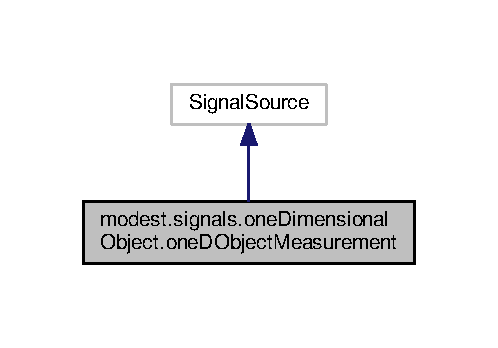
\includegraphics[width=239pt]{classmodest_1_1signals_1_1oneDimensionalObject_1_1oneDObjectMeasurement__coll__graph}
\end{center}
\end{figure}
\subsection*{Public Member Functions}
\begin{DoxyCompactItemize}
\item 
def \hyperlink{classmodest_1_1signals_1_1oneDimensionalObject_1_1oneDObjectMeasurement_aa7849d9c570738c30e90b37c975cc329}{\+\_\+\+\_\+init\+\_\+\+\_\+} (self, \hyperlink{classmodest_1_1signals_1_1oneDimensionalObject_1_1oneDObjectMeasurement_a998f41f9e1ef63fc336f4c1d52c1aa4b}{object\+ID})
\item 
def \hyperlink{classmodest_1_1signals_1_1oneDimensionalObject_1_1oneDObjectMeasurement_a357fb9341c6c3b09864cf24b038936bd}{compute\+Association\+Probability} (self, measurement, state\+Dict, validation\+Threshold=0)
\end{DoxyCompactItemize}
\subsection*{Public Attributes}
\begin{DoxyCompactItemize}
\item 
\hyperlink{classmodest_1_1signals_1_1oneDimensionalObject_1_1oneDObjectMeasurement_a998f41f9e1ef63fc336f4c1d52c1aa4b}{object\+ID}
\end{DoxyCompactItemize}


\subsection{Detailed Description}


Definition at line 5 of file one\+Dimensional\+Object.\+py.



\subsection{Constructor \& Destructor Documentation}
\index{modest\+::signals\+::one\+Dimensional\+Object\+::one\+D\+Object\+Measurement@{modest\+::signals\+::one\+Dimensional\+Object\+::one\+D\+Object\+Measurement}!\+\_\+\+\_\+init\+\_\+\+\_\+@{\+\_\+\+\_\+init\+\_\+\+\_\+}}
\index{\+\_\+\+\_\+init\+\_\+\+\_\+@{\+\_\+\+\_\+init\+\_\+\+\_\+}!modest\+::signals\+::one\+Dimensional\+Object\+::one\+D\+Object\+Measurement@{modest\+::signals\+::one\+Dimensional\+Object\+::one\+D\+Object\+Measurement}}
\subsubsection[{\texorpdfstring{\+\_\+\+\_\+init\+\_\+\+\_\+(self, object\+I\+D)}{__init__(self, objectID)}}]{\setlength{\rightskip}{0pt plus 5cm}def modest.\+signals.\+one\+Dimensional\+Object.\+one\+D\+Object\+Measurement.\+\_\+\+\_\+init\+\_\+\+\_\+ (
\begin{DoxyParamCaption}
\item[{}]{self, }
\item[{}]{object\+ID}
\end{DoxyParamCaption}
)}\hypertarget{classmodest_1_1signals_1_1oneDimensionalObject_1_1oneDObjectMeasurement_aa7849d9c570738c30e90b37c975cc329}{}\label{classmodest_1_1signals_1_1oneDimensionalObject_1_1oneDObjectMeasurement_aa7849d9c570738c30e90b37c975cc329}


Definition at line 6 of file one\+Dimensional\+Object.\+py.



\subsection{Member Function Documentation}
\index{modest\+::signals\+::one\+Dimensional\+Object\+::one\+D\+Object\+Measurement@{modest\+::signals\+::one\+Dimensional\+Object\+::one\+D\+Object\+Measurement}!compute\+Association\+Probability@{compute\+Association\+Probability}}
\index{compute\+Association\+Probability@{compute\+Association\+Probability}!modest\+::signals\+::one\+Dimensional\+Object\+::one\+D\+Object\+Measurement@{modest\+::signals\+::one\+Dimensional\+Object\+::one\+D\+Object\+Measurement}}
\subsubsection[{\texorpdfstring{compute\+Association\+Probability(self, measurement, state\+Dict, validation\+Threshold=0)}{computeAssociationProbability(self, measurement, stateDict, validationThreshold=0)}}]{\setlength{\rightskip}{0pt plus 5cm}def modest.\+signals.\+one\+Dimensional\+Object.\+one\+D\+Object\+Measurement.\+compute\+Association\+Probability (
\begin{DoxyParamCaption}
\item[{}]{self, }
\item[{}]{measurement, }
\item[{}]{state\+Dict, }
\item[{}]{validation\+Threshold = {\ttfamily 0}}
\end{DoxyParamCaption}
)}\hypertarget{classmodest_1_1signals_1_1oneDimensionalObject_1_1oneDObjectMeasurement_a357fb9341c6c3b09864cf24b038936bd}{}\label{classmodest_1_1signals_1_1oneDimensionalObject_1_1oneDObjectMeasurement_a357fb9341c6c3b09864cf24b038936bd}


Definition at line 10 of file one\+Dimensional\+Object.\+py.



\subsection{Member Data Documentation}
\index{modest\+::signals\+::one\+Dimensional\+Object\+::one\+D\+Object\+Measurement@{modest\+::signals\+::one\+Dimensional\+Object\+::one\+D\+Object\+Measurement}!object\+ID@{object\+ID}}
\index{object\+ID@{object\+ID}!modest\+::signals\+::one\+Dimensional\+Object\+::one\+D\+Object\+Measurement@{modest\+::signals\+::one\+Dimensional\+Object\+::one\+D\+Object\+Measurement}}
\subsubsection[{\texorpdfstring{object\+ID}{objectID}}]{\setlength{\rightskip}{0pt plus 5cm}modest.\+signals.\+one\+Dimensional\+Object.\+one\+D\+Object\+Measurement.\+object\+ID}\hypertarget{classmodest_1_1signals_1_1oneDimensionalObject_1_1oneDObjectMeasurement_a998f41f9e1ef63fc336f4c1d52c1aa4b}{}\label{classmodest_1_1signals_1_1oneDimensionalObject_1_1oneDObjectMeasurement_a998f41f9e1ef63fc336f4c1d52c1aa4b}


Definition at line 7 of file one\+Dimensional\+Object.\+py.



The documentation for this class was generated from the following file\+:\begin{DoxyCompactItemize}
\item 
modest/signals/\hyperlink{oneDimensionalObject_8py}{one\+Dimensional\+Object.\+py}\end{DoxyCompactItemize}

\hypertarget{classmodest_1_1substates_1_1oneDimensionalPositionVelocity_1_1oneDPositionVelocity}{}\section{modest.\+substates.\+one\+Dimensional\+Position\+Velocity.\+one\+D\+Position\+Velocity Class Reference}
\label{classmodest_1_1substates_1_1oneDimensionalPositionVelocity_1_1oneDPositionVelocity}\index{modest.\+substates.\+one\+Dimensional\+Position\+Velocity.\+one\+D\+Position\+Velocity@{modest.\+substates.\+one\+Dimensional\+Position\+Velocity.\+one\+D\+Position\+Velocity}}


Inheritance diagram for modest.\+substates.\+one\+Dimensional\+Position\+Velocity.\+one\+D\+Position\+Velocity\+:
\nopagebreak
\begin{figure}[H]
\begin{center}
\leavevmode
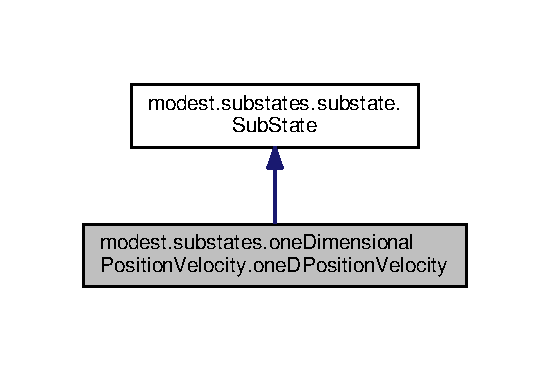
\includegraphics[width=264pt]{classmodest_1_1substates_1_1oneDimensionalPositionVelocity_1_1oneDPositionVelocity__inherit__graph}
\end{center}
\end{figure}


Collaboration diagram for modest.\+substates.\+one\+Dimensional\+Position\+Velocity.\+one\+D\+Position\+Velocity\+:
\nopagebreak
\begin{figure}[H]
\begin{center}
\leavevmode
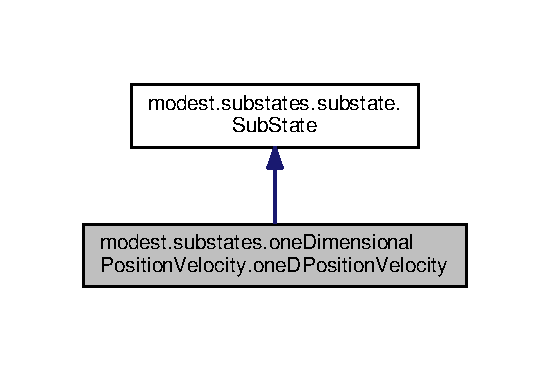
\includegraphics[width=264pt]{classmodest_1_1substates_1_1oneDimensionalPositionVelocity_1_1oneDPositionVelocity__coll__graph}
\end{center}
\end{figure}
\subsection*{Public Member Functions}
\begin{DoxyCompactItemize}
\item 
def \hyperlink{classmodest_1_1substates_1_1oneDimensionalPositionVelocity_1_1oneDPositionVelocity_a01dab857d13926a0297edd0e15fc4f55}{\+\_\+\+\_\+init\+\_\+\+\_\+} (self, \hyperlink{classmodest_1_1substates_1_1oneDimensionalPositionVelocity_1_1oneDPositionVelocity_a805e7dfe302ac83ca52c1b15b171b93e}{object\+ID}, \hyperlink{classmodest_1_1substates_1_1substate_1_1SubState_a38c12c9d0899bc1161f3502b584517a2}{state\+Vector\+History}, covariance\+Storage=\textquotesingle{}\hyperlink{classmodest_1_1substates_1_1substate_1_1SubState_a6e308aadd13962e476d2892ec728e3a5}{covariance}\textquotesingle{}, \hyperlink{classmodest_1_1substates_1_1oneDimensionalPositionVelocity_1_1oneDPositionVelocity_adfefff9b378df18fdb575973cdb6cb52}{bias\+State}=True, \hyperlink{classmodest_1_1substates_1_1oneDimensionalPositionVelocity_1_1oneDPositionVelocity_adafaa6e838c7ecf09b4397bf46310622}{artificial\+Bias\+Meas}=True, \hyperlink{classmodest_1_1substates_1_1oneDimensionalPositionVelocity_1_1oneDPositionVelocity_a4fc82761e11022f9643504aa5e2123b5}{bias\+State\+Time\+Constant}=0.\+9, \hyperlink{classmodest_1_1substates_1_1oneDimensionalPositionVelocity_1_1oneDPositionVelocity_ac365e7ee6e0ca28406ec88129d286429}{bias\+State\+Process\+Noise\+Var}=1e-\/3, bias\+Meas\+Var=1)
\item 
def \hyperlink{classmodest_1_1substates_1_1oneDimensionalPositionVelocity_1_1oneDPositionVelocity_af2b9f31a579e0cc41b96ecc8bbe37f2a}{store\+State\+Vector} (self, sv\+Dict)
\item 
def \hyperlink{classmodest_1_1substates_1_1oneDimensionalPositionVelocity_1_1oneDPositionVelocity_a4f45b205f5a2c41f82c8916d3afcbbce}{time\+Update} (self, dT, dynamics=None)
\item 
def \hyperlink{classmodest_1_1substates_1_1oneDimensionalPositionVelocity_1_1oneDPositionVelocity_a71b8ca17a8732b89e1dcaed2fcc5b3df}{get\+Measurement\+Matrices} (self, measurement, source=None)
\end{DoxyCompactItemize}
\begin{Indent}{\bf Mandatory Sub\+State Functions}\par
{\em The following functions are functions which are required for the Sub\+State to function as a sub-\/state in State.\+Modular\+Filter. }\begin{DoxyCompactItemize}
\item 
def \hyperlink{classmodest_1_1substates_1_1substate_1_1SubState_a1d8050de59c58969164f577899a55aa2}{get\+State\+Vector} (self, t=None)
\begin{DoxyCompactList}\small\item\em \hyperlink{classmodest_1_1substates_1_1substate_1_1SubState_a1d8050de59c58969164f577899a55aa2}{get\+State\+Vector} returns the most recent value of the state vector \end{DoxyCompactList}\item 
def \hyperlink{classmodest_1_1substates_1_1substate_1_1SubState_a6e308aadd13962e476d2892ec728e3a5}{covariance} (self)
\begin{DoxyCompactList}\small\item\em \hyperlink{classmodest_1_1substates_1_1substate_1_1SubState_a6e308aadd13962e476d2892ec728e3a5}{covariance} returns the \hyperlink{classmodest_1_1substates_1_1substate_1_1SubState}{Sub\+State} covariance matrix \end{DoxyCompactList}\item 
def \hyperlink{classmodest_1_1substates_1_1substate_1_1SubState_ab9027f6d1d7d57c47731612f519b7ee6}{dimension} (self)
\begin{DoxyCompactList}\small\item\em \hyperlink{classmodest_1_1substates_1_1substate_1_1SubState_ab9027f6d1d7d57c47731612f519b7ee6}{dimension} returns the dimension of the sub-\/state vector \end{DoxyCompactList}\end{DoxyCompactItemize}
\end{Indent}
\begin{Indent}{\bf Plotting Functions}\par
{\em These functions provide generalized plotting capabilities }\begin{DoxyCompactItemize}
\item 
def \hyperlink{classmodest_1_1substates_1_1substate_1_1SubState_a1adac64be88eab0a64bb952518c4268f}{initialize\+Real\+Time\+Plot} (self, plot\+Handle=None, axis\+Handle=None)
\item 
def \hyperlink{classmodest_1_1substates_1_1substate_1_1SubState_a2deb7d1ca3105eb20e50fa7e67298355}{real\+Time\+Plot} (self, normalized=True)
\item 
def \hyperlink{classmodest_1_1substates_1_1substate_1_1SubState_a643678c1193dd4029683a437e84229ac}{time\+History\+Plot} (self)
\item 
def \hyperlink{classmodest_1_1substates_1_1substate_1_1SubState_a1853d44036e3ed35ada02414ea29f8ab}{initialize\+Time\+History\+Plot} (self, plot\+Handle=None)
\end{DoxyCompactItemize}
\end{Indent}
\subsection*{Public Attributes}
\begin{DoxyCompactItemize}
\item 
\hyperlink{classmodest_1_1substates_1_1oneDimensionalPositionVelocity_1_1oneDPositionVelocity_adfefff9b378df18fdb575973cdb6cb52}{bias\+State}
\item 
\hyperlink{classmodest_1_1substates_1_1oneDimensionalPositionVelocity_1_1oneDPositionVelocity_a685cabbbc121aa8e0bca238d5dd1b370}{state\+Vector}
\item 
\hyperlink{classmodest_1_1substates_1_1oneDimensionalPositionVelocity_1_1oneDPositionVelocity_a805e7dfe302ac83ca52c1b15b171b93e}{object\+ID}
\item 
\hyperlink{classmodest_1_1substates_1_1oneDimensionalPositionVelocity_1_1oneDPositionVelocity_aeb9271160372d8db32e9317dd520bb8a}{velocity\+Var}
\item 
\hyperlink{classmodest_1_1substates_1_1oneDimensionalPositionVelocity_1_1oneDPositionVelocity_a4fa306721c79ec47a2e56d366e68002b}{position\+Var}
\item 
\hyperlink{classmodest_1_1substates_1_1oneDimensionalPositionVelocity_1_1oneDPositionVelocity_a11e9f155c003f833abc8dd013a04588d}{current\+Position}
\item 
\hyperlink{classmodest_1_1substates_1_1oneDimensionalPositionVelocity_1_1oneDPositionVelocity_a111816573a8073e5c0d9d04754480592}{current\+Velocity}
\item 
\hyperlink{classmodest_1_1substates_1_1oneDimensionalPositionVelocity_1_1oneDPositionVelocity_a57a153463c607dec6f91d0ce735eb5a9}{current\+Bias\+State}
\item 
\hyperlink{classmodest_1_1substates_1_1oneDimensionalPositionVelocity_1_1oneDPositionVelocity_adafaa6e838c7ecf09b4397bf46310622}{artificial\+Bias\+Meas}
\item 
\hyperlink{classmodest_1_1substates_1_1oneDimensionalPositionVelocity_1_1oneDPositionVelocity_ac365e7ee6e0ca28406ec88129d286429}{bias\+State\+Process\+Noise\+Var}
\item 
\hyperlink{classmodest_1_1substates_1_1oneDimensionalPositionVelocity_1_1oneDPositionVelocity_a4fc82761e11022f9643504aa5e2123b5}{bias\+State\+Time\+Constant}
\item 
\hyperlink{classmodest_1_1substates_1_1oneDimensionalPositionVelocity_1_1oneDPositionVelocity_a2666c203f3b0af4e17069ad5c80072c2}{artificial\+Bias\+Meas\+Var}
\item 
\hyperlink{classmodest_1_1substates_1_1substate_1_1SubState_a38c12c9d0899bc1161f3502b584517a2}{state\+Vector\+History}
\begin{DoxyCompactList}\small\item\em Stores the time-\/history of the sub-\/state state vector. \end{DoxyCompactList}\item 
\hyperlink{classmodest_1_1substates_1_1substate_1_1SubState_a9b7a77e3b7dc14fc85962cda84e8cd58}{time\+List}
\item 
\hyperlink{classmodest_1_1substates_1_1substate_1_1SubState_a37ded775b84cea85b4dce0f1b16286c4}{R\+T\+Plot\+Handle}
\begin{DoxyCompactList}\small\item\em Stores handle for real-\/time plotting. \end{DoxyCompactList}\item 
\hyperlink{classmodest_1_1substates_1_1substate_1_1SubState_af1d5d3bbdf73cf1e78925c835f1c616e}{T\+H\+Plot\+Handle}
\item 
\hyperlink{classmodest_1_1substates_1_1substate_1_1SubState_a9fefae1facc797a1132fb61a55e9ffa1}{R\+T\+Plot\+Data}
\item 
\hyperlink{classmodest_1_1substates_1_1substate_1_1SubState_a497ccbb6658589b02568e87c6382222e}{R\+T\+Paxis\+Handle}
\item 
\hyperlink{classmodest_1_1substates_1_1substate_1_1SubState_a22c12497c37f47d54d4ea909f6423222}{T\+H\+Paxis\+List}
\item 
\hyperlink{classmodest_1_1substates_1_1substate_1_1SubState_a0e1d545f7ede186d89db38ca613633cf}{T\+H\+Plot\+Data\+List}
\item 
\hyperlink{classmodest_1_1substates_1_1substate_1_1SubState_a9659535520a27090d79be1957ecce2eb}{T\+H\+Plot\+Object\+List}
\end{DoxyCompactItemize}


\subsection{Detailed Description}


Definition at line 6 of file one\+Dimensional\+Position\+Velocity.\+py.



\subsection{Constructor \& Destructor Documentation}
\index{modest\+::substates\+::one\+Dimensional\+Position\+Velocity\+::one\+D\+Position\+Velocity@{modest\+::substates\+::one\+Dimensional\+Position\+Velocity\+::one\+D\+Position\+Velocity}!\+\_\+\+\_\+init\+\_\+\+\_\+@{\+\_\+\+\_\+init\+\_\+\+\_\+}}
\index{\+\_\+\+\_\+init\+\_\+\+\_\+@{\+\_\+\+\_\+init\+\_\+\+\_\+}!modest\+::substates\+::one\+Dimensional\+Position\+Velocity\+::one\+D\+Position\+Velocity@{modest\+::substates\+::one\+Dimensional\+Position\+Velocity\+::one\+D\+Position\+Velocity}}
\subsubsection[{\texorpdfstring{\+\_\+\+\_\+init\+\_\+\+\_\+(self, object\+I\+D, state\+Vector\+History, covariance\+Storage=\textquotesingle{}covariance\textquotesingle{}, bias\+State=\+True, artificial\+Bias\+Meas=\+True, bias\+State\+Time\+Constant=0.\+9, bias\+State\+Process\+Noise\+Var=1e-\/3, bias\+Meas\+Var=1)}{__init__(self, objectID, stateVectorHistory, covarianceStorage='covariance', biasState=True, artificialBiasMeas=True, biasStateTimeConstant=0.9, biasStateProcessNoiseVar=1e-3, biasMeasVar=1)}}]{\setlength{\rightskip}{0pt plus 5cm}def modest.\+substates.\+one\+Dimensional\+Position\+Velocity.\+one\+D\+Position\+Velocity.\+\_\+\+\_\+init\+\_\+\+\_\+ (
\begin{DoxyParamCaption}
\item[{}]{self, }
\item[{}]{object\+ID, }
\item[{}]{state\+Vector\+History, }
\item[{}]{covariance\+Storage = {\ttfamily \textquotesingle{}{\bf covariance}\textquotesingle{}}, }
\item[{}]{bias\+State = {\ttfamily True}, }
\item[{}]{artificial\+Bias\+Meas = {\ttfamily True}, }
\item[{}]{bias\+State\+Time\+Constant = {\ttfamily 0.9}, }
\item[{}]{bias\+State\+Process\+Noise\+Var = {\ttfamily 1e-\/3}, }
\item[{}]{bias\+Meas\+Var = {\ttfamily 1}}
\end{DoxyParamCaption}
)}\hypertarget{classmodest_1_1substates_1_1oneDimensionalPositionVelocity_1_1oneDPositionVelocity_a01dab857d13926a0297edd0e15fc4f55}{}\label{classmodest_1_1substates_1_1oneDimensionalPositionVelocity_1_1oneDPositionVelocity_a01dab857d13926a0297edd0e15fc4f55}


Definition at line 17 of file one\+Dimensional\+Position\+Velocity.\+py.



\subsection{Member Function Documentation}
\index{modest\+::substates\+::one\+Dimensional\+Position\+Velocity\+::one\+D\+Position\+Velocity@{modest\+::substates\+::one\+Dimensional\+Position\+Velocity\+::one\+D\+Position\+Velocity}!covariance@{covariance}}
\index{covariance@{covariance}!modest\+::substates\+::one\+Dimensional\+Position\+Velocity\+::one\+D\+Position\+Velocity@{modest\+::substates\+::one\+Dimensional\+Position\+Velocity\+::one\+D\+Position\+Velocity}}
\subsubsection[{\texorpdfstring{covariance(self)}{covariance(self)}}]{\setlength{\rightskip}{0pt plus 5cm}def modest.\+substates.\+substate.\+Sub\+State.\+covariance (
\begin{DoxyParamCaption}
\item[{}]{self}
\end{DoxyParamCaption}
)\hspace{0.3cm}{\ttfamily [inherited]}}\hypertarget{classmodest_1_1substates_1_1substate_1_1SubState_a6e308aadd13962e476d2892ec728e3a5}{}\label{classmodest_1_1substates_1_1substate_1_1SubState_a6e308aadd13962e476d2892ec728e3a5}


\hyperlink{classmodest_1_1substates_1_1substate_1_1SubState_a6e308aadd13962e476d2892ec728e3a5}{covariance} returns the \hyperlink{classmodest_1_1substates_1_1substate_1_1SubState}{Sub\+State} covariance matrix 

The \hyperlink{classmodest_1_1substates_1_1substate_1_1SubState_a6e308aadd13962e476d2892ec728e3a5}{covariance} method returns the covariance of the estimate of the substate.

\begin{DoxyRefDesc}{Todo}
\item[\hyperlink{todo__todo000001}{Todo}]Currently, this method only returns the covariance of the most recent state estimate. Ideally, there should be an optional time parameter which would allow the user to get the covaraince matrix at a specified time (or the closest to that specified time).\end{DoxyRefDesc}



\begin{DoxyParams}{Parameters}
{\em self} & The object pointer\\
\hline
\end{DoxyParams}
\begin{DoxyReturn}{Returns}
Returns the covaraince matrix 
\end{DoxyReturn}


Definition at line 185 of file substate.\+py.

\index{modest\+::substates\+::one\+Dimensional\+Position\+Velocity\+::one\+D\+Position\+Velocity@{modest\+::substates\+::one\+Dimensional\+Position\+Velocity\+::one\+D\+Position\+Velocity}!dimension@{dimension}}
\index{dimension@{dimension}!modest\+::substates\+::one\+Dimensional\+Position\+Velocity\+::one\+D\+Position\+Velocity@{modest\+::substates\+::one\+Dimensional\+Position\+Velocity\+::one\+D\+Position\+Velocity}}
\subsubsection[{\texorpdfstring{dimension(self)}{dimension(self)}}]{\setlength{\rightskip}{0pt plus 5cm}def modest.\+substates.\+substate.\+Sub\+State.\+dimension (
\begin{DoxyParamCaption}
\item[{}]{self}
\end{DoxyParamCaption}
)\hspace{0.3cm}{\ttfamily [inherited]}}\hypertarget{classmodest_1_1substates_1_1substate_1_1SubState_ab9027f6d1d7d57c47731612f519b7ee6}{}\label{classmodest_1_1substates_1_1substate_1_1SubState_ab9027f6d1d7d57c47731612f519b7ee6}


\hyperlink{classmodest_1_1substates_1_1substate_1_1SubState_ab9027f6d1d7d57c47731612f519b7ee6}{dimension} returns the dimension of the sub-\/state vector 

The \hyperlink{classmodest_1_1substates_1_1substate_1_1SubState_ab9027f6d1d7d57c47731612f519b7ee6}{dimension} method returns the dimension of the sub-\/state vector estimated by the \hyperlink{classmodest_1_1substates_1_1substate_1_1SubState}{Sub\+State}. This is the dimension as seen by the Modular\+Filter estimator.

The default implementation is to return the class variable \hyperlink{classmodest_1_1substates_1_1substate_1_1SubState_a5b1c0756a69da7f293a415c7d2d77843}{\+\_\+\+\_\+dimension\+\_\+\+\_\+}, which is saved at initialization. This is designated as a \char`\"{}protected\char`\"{} variable, and should not change during the course of the \hyperlink{classmodest_1_1substates_1_1substate_1_1SubState}{Sub\+State}\textquotesingle{}s lifetime. If child class overwrites this implementation, care should be taken to ensure that the value returned by \hyperlink{classmodest_1_1substates_1_1substate_1_1SubState_ab9027f6d1d7d57c47731612f519b7ee6}{dimension} does not change over \hyperlink{classmodest_1_1substates_1_1substate_1_1SubState}{Sub\+State} object lifetime.

For \hyperlink{classmodest_1_1substates_1_1substate_1_1SubState}{Sub\+State} objects with auxilary states, or other quantities related to the state vector but not directly estimated by the Modular\+Filter, \hyperlink{classmodest_1_1substates_1_1substate_1_1SubState_ab9027f6d1d7d57c47731612f519b7ee6}{dimension} should not count these states as part of the total dimension.


\begin{DoxyParams}{Parameters}
{\em self} & The object pointer\\
\hline
\end{DoxyParams}
\begin{DoxyReturn}{Returns}
Returns the dimension of state vector 
\end{DoxyReturn}


Definition at line 211 of file substate.\+py.

\index{modest\+::substates\+::one\+Dimensional\+Position\+Velocity\+::one\+D\+Position\+Velocity@{modest\+::substates\+::one\+Dimensional\+Position\+Velocity\+::one\+D\+Position\+Velocity}!get\+Measurement\+Matrices@{get\+Measurement\+Matrices}}
\index{get\+Measurement\+Matrices@{get\+Measurement\+Matrices}!modest\+::substates\+::one\+Dimensional\+Position\+Velocity\+::one\+D\+Position\+Velocity@{modest\+::substates\+::one\+Dimensional\+Position\+Velocity\+::one\+D\+Position\+Velocity}}
\subsubsection[{\texorpdfstring{get\+Measurement\+Matrices(self, measurement, source=\+None)}{getMeasurementMatrices(self, measurement, source=None)}}]{\setlength{\rightskip}{0pt plus 5cm}def modest.\+substates.\+one\+Dimensional\+Position\+Velocity.\+one\+D\+Position\+Velocity.\+get\+Measurement\+Matrices (
\begin{DoxyParamCaption}
\item[{}]{self, }
\item[{}]{measurement, }
\item[{}]{source = {\ttfamily None}}
\end{DoxyParamCaption}
)}\hypertarget{classmodest_1_1substates_1_1oneDimensionalPositionVelocity_1_1oneDPositionVelocity_a71b8ca17a8732b89e1dcaed2fcc5b3df}{}\label{classmodest_1_1substates_1_1oneDimensionalPositionVelocity_1_1oneDPositionVelocity_a71b8ca17a8732b89e1dcaed2fcc5b3df}


Definition at line 118 of file one\+Dimensional\+Position\+Velocity.\+py.

\index{modest\+::substates\+::one\+Dimensional\+Position\+Velocity\+::one\+D\+Position\+Velocity@{modest\+::substates\+::one\+Dimensional\+Position\+Velocity\+::one\+D\+Position\+Velocity}!get\+State\+Vector@{get\+State\+Vector}}
\index{get\+State\+Vector@{get\+State\+Vector}!modest\+::substates\+::one\+Dimensional\+Position\+Velocity\+::one\+D\+Position\+Velocity@{modest\+::substates\+::one\+Dimensional\+Position\+Velocity\+::one\+D\+Position\+Velocity}}
\subsubsection[{\texorpdfstring{get\+State\+Vector(self, t=\+None)}{getStateVector(self, t=None)}}]{\setlength{\rightskip}{0pt plus 5cm}def modest.\+substates.\+substate.\+Sub\+State.\+get\+State\+Vector (
\begin{DoxyParamCaption}
\item[{}]{self, }
\item[{}]{t = {\ttfamily None}}
\end{DoxyParamCaption}
)\hspace{0.3cm}{\ttfamily [inherited]}}\hypertarget{classmodest_1_1substates_1_1substate_1_1SubState_a1d8050de59c58969164f577899a55aa2}{}\label{classmodest_1_1substates_1_1substate_1_1SubState_a1d8050de59c58969164f577899a55aa2}


\hyperlink{classmodest_1_1substates_1_1substate_1_1SubState_a1d8050de59c58969164f577899a55aa2}{get\+State\+Vector} returns the most recent value of the state vector 

The \hyperlink{classmodest_1_1substates_1_1substate_1_1SubState_a1d8050de59c58969164f577899a55aa2}{get\+State\+Vector} method is responsible for returning a dictionary object containing, at minimim, the following items\+:


\begin{DoxyItemize}
\item \textquotesingle{}state\+Vector\textquotesingle{}\+: A length \hyperlink{classmodest_1_1substates_1_1substate_1_1SubState_ab9027f6d1d7d57c47731612f519b7ee6}{dimension} array containing the most recent state vector estimate
\item \textquotesingle{}covariance\textquotesingle{}\+: A (\hyperlink{classmodest_1_1substates_1_1substate_1_1SubState_ab9027f6d1d7d57c47731612f519b7ee6}{dimension} x \hyperlink{classmodest_1_1substates_1_1substate_1_1SubState_ab9027f6d1d7d57c47731612f519b7ee6}{dimension}) array containing the most recent covariance matrix
\item \textquotesingle{}a\+Priori\textquotesingle{}\+: A boolean indicating if the most recent estimate is the
\item result of a time update (a\+Priori=True) or a measurement update (a\+Priori=False)
\end{DoxyItemize}

This function can be used as-\/is, or can be overloaded to perform additional tasks specific to the substate.


\begin{DoxyParams}{Parameters}
{\em self} & The object pointer\\
\hline
\end{DoxyParams}
\begin{DoxyReturn}{Returns}
The dictionary containing the state vector, covariance matrix, and a\+Priori status 
\end{DoxyReturn}


Definition at line 135 of file substate.\+py.

\index{modest\+::substates\+::one\+Dimensional\+Position\+Velocity\+::one\+D\+Position\+Velocity@{modest\+::substates\+::one\+Dimensional\+Position\+Velocity\+::one\+D\+Position\+Velocity}!initialize\+Real\+Time\+Plot@{initialize\+Real\+Time\+Plot}}
\index{initialize\+Real\+Time\+Plot@{initialize\+Real\+Time\+Plot}!modest\+::substates\+::one\+Dimensional\+Position\+Velocity\+::one\+D\+Position\+Velocity@{modest\+::substates\+::one\+Dimensional\+Position\+Velocity\+::one\+D\+Position\+Velocity}}
\subsubsection[{\texorpdfstring{initialize\+Real\+Time\+Plot(self, plot\+Handle=\+None, axis\+Handle=\+None)}{initializeRealTimePlot(self, plotHandle=None, axisHandle=None)}}]{\setlength{\rightskip}{0pt plus 5cm}def modest.\+substates.\+substate.\+Sub\+State.\+initialize\+Real\+Time\+Plot (
\begin{DoxyParamCaption}
\item[{}]{self, }
\item[{}]{plot\+Handle = {\ttfamily None}, }
\item[{}]{axis\+Handle = {\ttfamily None}}
\end{DoxyParamCaption}
)\hspace{0.3cm}{\ttfamily [inherited]}}\hypertarget{classmodest_1_1substates_1_1substate_1_1SubState_a1adac64be88eab0a64bb952518c4268f}{}\label{classmodest_1_1substates_1_1substate_1_1SubState_a1adac64be88eab0a64bb952518c4268f}


Definition at line 271 of file substate.\+py.

\index{modest\+::substates\+::one\+Dimensional\+Position\+Velocity\+::one\+D\+Position\+Velocity@{modest\+::substates\+::one\+Dimensional\+Position\+Velocity\+::one\+D\+Position\+Velocity}!initialize\+Time\+History\+Plot@{initialize\+Time\+History\+Plot}}
\index{initialize\+Time\+History\+Plot@{initialize\+Time\+History\+Plot}!modest\+::substates\+::one\+Dimensional\+Position\+Velocity\+::one\+D\+Position\+Velocity@{modest\+::substates\+::one\+Dimensional\+Position\+Velocity\+::one\+D\+Position\+Velocity}}
\subsubsection[{\texorpdfstring{initialize\+Time\+History\+Plot(self, plot\+Handle=\+None)}{initializeTimeHistoryPlot(self, plotHandle=None)}}]{\setlength{\rightskip}{0pt plus 5cm}def modest.\+substates.\+substate.\+Sub\+State.\+initialize\+Time\+History\+Plot (
\begin{DoxyParamCaption}
\item[{}]{self, }
\item[{}]{plot\+Handle = {\ttfamily None}}
\end{DoxyParamCaption}
)\hspace{0.3cm}{\ttfamily [inherited]}}\hypertarget{classmodest_1_1substates_1_1substate_1_1SubState_a1853d44036e3ed35ada02414ea29f8ab}{}\label{classmodest_1_1substates_1_1substate_1_1SubState_a1853d44036e3ed35ada02414ea29f8ab}


Definition at line 350 of file substate.\+py.

\index{modest\+::substates\+::one\+Dimensional\+Position\+Velocity\+::one\+D\+Position\+Velocity@{modest\+::substates\+::one\+Dimensional\+Position\+Velocity\+::one\+D\+Position\+Velocity}!real\+Time\+Plot@{real\+Time\+Plot}}
\index{real\+Time\+Plot@{real\+Time\+Plot}!modest\+::substates\+::one\+Dimensional\+Position\+Velocity\+::one\+D\+Position\+Velocity@{modest\+::substates\+::one\+Dimensional\+Position\+Velocity\+::one\+D\+Position\+Velocity}}
\subsubsection[{\texorpdfstring{real\+Time\+Plot(self, normalized=\+True)}{realTimePlot(self, normalized=True)}}]{\setlength{\rightskip}{0pt plus 5cm}def modest.\+substates.\+substate.\+Sub\+State.\+real\+Time\+Plot (
\begin{DoxyParamCaption}
\item[{}]{self, }
\item[{}]{normalized = {\ttfamily True}}
\end{DoxyParamCaption}
)\hspace{0.3cm}{\ttfamily [inherited]}}\hypertarget{classmodest_1_1substates_1_1substate_1_1SubState_a2deb7d1ca3105eb20e50fa7e67298355}{}\label{classmodest_1_1substates_1_1substate_1_1SubState_a2deb7d1ca3105eb20e50fa7e67298355}


Definition at line 298 of file substate.\+py.

\index{modest\+::substates\+::one\+Dimensional\+Position\+Velocity\+::one\+D\+Position\+Velocity@{modest\+::substates\+::one\+Dimensional\+Position\+Velocity\+::one\+D\+Position\+Velocity}!store\+State\+Vector@{store\+State\+Vector}}
\index{store\+State\+Vector@{store\+State\+Vector}!modest\+::substates\+::one\+Dimensional\+Position\+Velocity\+::one\+D\+Position\+Velocity@{modest\+::substates\+::one\+Dimensional\+Position\+Velocity\+::one\+D\+Position\+Velocity}}
\subsubsection[{\texorpdfstring{store\+State\+Vector(self, sv\+Dict)}{storeStateVector(self, svDict)}}]{\setlength{\rightskip}{0pt plus 5cm}def modest.\+substates.\+one\+Dimensional\+Position\+Velocity.\+one\+D\+Position\+Velocity.\+store\+State\+Vector (
\begin{DoxyParamCaption}
\item[{}]{self, }
\item[{}]{sv\+Dict}
\end{DoxyParamCaption}
)}\hypertarget{classmodest_1_1substates_1_1oneDimensionalPositionVelocity_1_1oneDPositionVelocity_af2b9f31a579e0cc41b96ecc8bbe37f2a}{}\label{classmodest_1_1substates_1_1oneDimensionalPositionVelocity_1_1oneDPositionVelocity_af2b9f31a579e0cc41b96ecc8bbe37f2a}


Definition at line 48 of file one\+Dimensional\+Position\+Velocity.\+py.

\index{modest\+::substates\+::one\+Dimensional\+Position\+Velocity\+::one\+D\+Position\+Velocity@{modest\+::substates\+::one\+Dimensional\+Position\+Velocity\+::one\+D\+Position\+Velocity}!time\+History\+Plot@{time\+History\+Plot}}
\index{time\+History\+Plot@{time\+History\+Plot}!modest\+::substates\+::one\+Dimensional\+Position\+Velocity\+::one\+D\+Position\+Velocity@{modest\+::substates\+::one\+Dimensional\+Position\+Velocity\+::one\+D\+Position\+Velocity}}
\subsubsection[{\texorpdfstring{time\+History\+Plot(self)}{timeHistoryPlot(self)}}]{\setlength{\rightskip}{0pt plus 5cm}def modest.\+substates.\+substate.\+Sub\+State.\+time\+History\+Plot (
\begin{DoxyParamCaption}
\item[{}]{self}
\end{DoxyParamCaption}
)\hspace{0.3cm}{\ttfamily [inherited]}}\hypertarget{classmodest_1_1substates_1_1substate_1_1SubState_a643678c1193dd4029683a437e84229ac}{}\label{classmodest_1_1substates_1_1substate_1_1SubState_a643678c1193dd4029683a437e84229ac}


Definition at line 328 of file substate.\+py.

\index{modest\+::substates\+::one\+Dimensional\+Position\+Velocity\+::one\+D\+Position\+Velocity@{modest\+::substates\+::one\+Dimensional\+Position\+Velocity\+::one\+D\+Position\+Velocity}!time\+Update@{time\+Update}}
\index{time\+Update@{time\+Update}!modest\+::substates\+::one\+Dimensional\+Position\+Velocity\+::one\+D\+Position\+Velocity@{modest\+::substates\+::one\+Dimensional\+Position\+Velocity\+::one\+D\+Position\+Velocity}}
\subsubsection[{\texorpdfstring{time\+Update(self, d\+T, dynamics=\+None)}{timeUpdate(self, dT, dynamics=None)}}]{\setlength{\rightskip}{0pt plus 5cm}def modest.\+substates.\+one\+Dimensional\+Position\+Velocity.\+one\+D\+Position\+Velocity.\+time\+Update (
\begin{DoxyParamCaption}
\item[{}]{self, }
\item[{}]{dT, }
\item[{}]{dynamics = {\ttfamily None}}
\end{DoxyParamCaption}
)}\hypertarget{classmodest_1_1substates_1_1oneDimensionalPositionVelocity_1_1oneDPositionVelocity_a4f45b205f5a2c41f82c8916d3afcbbce}{}\label{classmodest_1_1substates_1_1oneDimensionalPositionVelocity_1_1oneDPositionVelocity_a4f45b205f5a2c41f82c8916d3afcbbce}


Definition at line 74 of file one\+Dimensional\+Position\+Velocity.\+py.



\subsection{Member Data Documentation}
\index{modest\+::substates\+::one\+Dimensional\+Position\+Velocity\+::one\+D\+Position\+Velocity@{modest\+::substates\+::one\+Dimensional\+Position\+Velocity\+::one\+D\+Position\+Velocity}!artificial\+Bias\+Meas@{artificial\+Bias\+Meas}}
\index{artificial\+Bias\+Meas@{artificial\+Bias\+Meas}!modest\+::substates\+::one\+Dimensional\+Position\+Velocity\+::one\+D\+Position\+Velocity@{modest\+::substates\+::one\+Dimensional\+Position\+Velocity\+::one\+D\+Position\+Velocity}}
\subsubsection[{\texorpdfstring{artificial\+Bias\+Meas}{artificialBiasMeas}}]{\setlength{\rightskip}{0pt plus 5cm}modest.\+substates.\+one\+Dimensional\+Position\+Velocity.\+one\+D\+Position\+Velocity.\+artificial\+Bias\+Meas}\hypertarget{classmodest_1_1substates_1_1oneDimensionalPositionVelocity_1_1oneDPositionVelocity_adafaa6e838c7ecf09b4397bf46310622}{}\label{classmodest_1_1substates_1_1oneDimensionalPositionVelocity_1_1oneDPositionVelocity_adafaa6e838c7ecf09b4397bf46310622}


Definition at line 42 of file one\+Dimensional\+Position\+Velocity.\+py.

\index{modest\+::substates\+::one\+Dimensional\+Position\+Velocity\+::one\+D\+Position\+Velocity@{modest\+::substates\+::one\+Dimensional\+Position\+Velocity\+::one\+D\+Position\+Velocity}!artificial\+Bias\+Meas\+Var@{artificial\+Bias\+Meas\+Var}}
\index{artificial\+Bias\+Meas\+Var@{artificial\+Bias\+Meas\+Var}!modest\+::substates\+::one\+Dimensional\+Position\+Velocity\+::one\+D\+Position\+Velocity@{modest\+::substates\+::one\+Dimensional\+Position\+Velocity\+::one\+D\+Position\+Velocity}}
\subsubsection[{\texorpdfstring{artificial\+Bias\+Meas\+Var}{artificialBiasMeasVar}}]{\setlength{\rightskip}{0pt plus 5cm}modest.\+substates.\+one\+Dimensional\+Position\+Velocity.\+one\+D\+Position\+Velocity.\+artificial\+Bias\+Meas\+Var}\hypertarget{classmodest_1_1substates_1_1oneDimensionalPositionVelocity_1_1oneDPositionVelocity_a2666c203f3b0af4e17069ad5c80072c2}{}\label{classmodest_1_1substates_1_1oneDimensionalPositionVelocity_1_1oneDPositionVelocity_a2666c203f3b0af4e17069ad5c80072c2}


Definition at line 46 of file one\+Dimensional\+Position\+Velocity.\+py.

\index{modest\+::substates\+::one\+Dimensional\+Position\+Velocity\+::one\+D\+Position\+Velocity@{modest\+::substates\+::one\+Dimensional\+Position\+Velocity\+::one\+D\+Position\+Velocity}!bias\+State@{bias\+State}}
\index{bias\+State@{bias\+State}!modest\+::substates\+::one\+Dimensional\+Position\+Velocity\+::one\+D\+Position\+Velocity@{modest\+::substates\+::one\+Dimensional\+Position\+Velocity\+::one\+D\+Position\+Velocity}}
\subsubsection[{\texorpdfstring{bias\+State}{biasState}}]{\setlength{\rightskip}{0pt plus 5cm}modest.\+substates.\+one\+Dimensional\+Position\+Velocity.\+one\+D\+Position\+Velocity.\+bias\+State}\hypertarget{classmodest_1_1substates_1_1oneDimensionalPositionVelocity_1_1oneDPositionVelocity_adfefff9b378df18fdb575973cdb6cb52}{}\label{classmodest_1_1substates_1_1oneDimensionalPositionVelocity_1_1oneDPositionVelocity_adfefff9b378df18fdb575973cdb6cb52}


Definition at line 23 of file one\+Dimensional\+Position\+Velocity.\+py.

\index{modest\+::substates\+::one\+Dimensional\+Position\+Velocity\+::one\+D\+Position\+Velocity@{modest\+::substates\+::one\+Dimensional\+Position\+Velocity\+::one\+D\+Position\+Velocity}!bias\+State\+Process\+Noise\+Var@{bias\+State\+Process\+Noise\+Var}}
\index{bias\+State\+Process\+Noise\+Var@{bias\+State\+Process\+Noise\+Var}!modest\+::substates\+::one\+Dimensional\+Position\+Velocity\+::one\+D\+Position\+Velocity@{modest\+::substates\+::one\+Dimensional\+Position\+Velocity\+::one\+D\+Position\+Velocity}}
\subsubsection[{\texorpdfstring{bias\+State\+Process\+Noise\+Var}{biasStateProcessNoiseVar}}]{\setlength{\rightskip}{0pt plus 5cm}modest.\+substates.\+one\+Dimensional\+Position\+Velocity.\+one\+D\+Position\+Velocity.\+bias\+State\+Process\+Noise\+Var}\hypertarget{classmodest_1_1substates_1_1oneDimensionalPositionVelocity_1_1oneDPositionVelocity_ac365e7ee6e0ca28406ec88129d286429}{}\label{classmodest_1_1substates_1_1oneDimensionalPositionVelocity_1_1oneDPositionVelocity_ac365e7ee6e0ca28406ec88129d286429}


Definition at line 44 of file one\+Dimensional\+Position\+Velocity.\+py.

\index{modest\+::substates\+::one\+Dimensional\+Position\+Velocity\+::one\+D\+Position\+Velocity@{modest\+::substates\+::one\+Dimensional\+Position\+Velocity\+::one\+D\+Position\+Velocity}!bias\+State\+Time\+Constant@{bias\+State\+Time\+Constant}}
\index{bias\+State\+Time\+Constant@{bias\+State\+Time\+Constant}!modest\+::substates\+::one\+Dimensional\+Position\+Velocity\+::one\+D\+Position\+Velocity@{modest\+::substates\+::one\+Dimensional\+Position\+Velocity\+::one\+D\+Position\+Velocity}}
\subsubsection[{\texorpdfstring{bias\+State\+Time\+Constant}{biasStateTimeConstant}}]{\setlength{\rightskip}{0pt plus 5cm}modest.\+substates.\+one\+Dimensional\+Position\+Velocity.\+one\+D\+Position\+Velocity.\+bias\+State\+Time\+Constant}\hypertarget{classmodest_1_1substates_1_1oneDimensionalPositionVelocity_1_1oneDPositionVelocity_a4fc82761e11022f9643504aa5e2123b5}{}\label{classmodest_1_1substates_1_1oneDimensionalPositionVelocity_1_1oneDPositionVelocity_a4fc82761e11022f9643504aa5e2123b5}


Definition at line 45 of file one\+Dimensional\+Position\+Velocity.\+py.

\index{modest\+::substates\+::one\+Dimensional\+Position\+Velocity\+::one\+D\+Position\+Velocity@{modest\+::substates\+::one\+Dimensional\+Position\+Velocity\+::one\+D\+Position\+Velocity}!current\+Bias\+State@{current\+Bias\+State}}
\index{current\+Bias\+State@{current\+Bias\+State}!modest\+::substates\+::one\+Dimensional\+Position\+Velocity\+::one\+D\+Position\+Velocity@{modest\+::substates\+::one\+Dimensional\+Position\+Velocity\+::one\+D\+Position\+Velocity}}
\subsubsection[{\texorpdfstring{current\+Bias\+State}{currentBiasState}}]{\setlength{\rightskip}{0pt plus 5cm}modest.\+substates.\+one\+Dimensional\+Position\+Velocity.\+one\+D\+Position\+Velocity.\+current\+Bias\+State}\hypertarget{classmodest_1_1substates_1_1oneDimensionalPositionVelocity_1_1oneDPositionVelocity_a57a153463c607dec6f91d0ce735eb5a9}{}\label{classmodest_1_1substates_1_1oneDimensionalPositionVelocity_1_1oneDPositionVelocity_a57a153463c607dec6f91d0ce735eb5a9}


Definition at line 40 of file one\+Dimensional\+Position\+Velocity.\+py.

\index{modest\+::substates\+::one\+Dimensional\+Position\+Velocity\+::one\+D\+Position\+Velocity@{modest\+::substates\+::one\+Dimensional\+Position\+Velocity\+::one\+D\+Position\+Velocity}!current\+Position@{current\+Position}}
\index{current\+Position@{current\+Position}!modest\+::substates\+::one\+Dimensional\+Position\+Velocity\+::one\+D\+Position\+Velocity@{modest\+::substates\+::one\+Dimensional\+Position\+Velocity\+::one\+D\+Position\+Velocity}}
\subsubsection[{\texorpdfstring{current\+Position}{currentPosition}}]{\setlength{\rightskip}{0pt plus 5cm}modest.\+substates.\+one\+Dimensional\+Position\+Velocity.\+one\+D\+Position\+Velocity.\+current\+Position}\hypertarget{classmodest_1_1substates_1_1oneDimensionalPositionVelocity_1_1oneDPositionVelocity_a11e9f155c003f833abc8dd013a04588d}{}\label{classmodest_1_1substates_1_1oneDimensionalPositionVelocity_1_1oneDPositionVelocity_a11e9f155c003f833abc8dd013a04588d}


Definition at line 38 of file one\+Dimensional\+Position\+Velocity.\+py.

\index{modest\+::substates\+::one\+Dimensional\+Position\+Velocity\+::one\+D\+Position\+Velocity@{modest\+::substates\+::one\+Dimensional\+Position\+Velocity\+::one\+D\+Position\+Velocity}!current\+Velocity@{current\+Velocity}}
\index{current\+Velocity@{current\+Velocity}!modest\+::substates\+::one\+Dimensional\+Position\+Velocity\+::one\+D\+Position\+Velocity@{modest\+::substates\+::one\+Dimensional\+Position\+Velocity\+::one\+D\+Position\+Velocity}}
\subsubsection[{\texorpdfstring{current\+Velocity}{currentVelocity}}]{\setlength{\rightskip}{0pt plus 5cm}modest.\+substates.\+one\+Dimensional\+Position\+Velocity.\+one\+D\+Position\+Velocity.\+current\+Velocity}\hypertarget{classmodest_1_1substates_1_1oneDimensionalPositionVelocity_1_1oneDPositionVelocity_a111816573a8073e5c0d9d04754480592}{}\label{classmodest_1_1substates_1_1oneDimensionalPositionVelocity_1_1oneDPositionVelocity_a111816573a8073e5c0d9d04754480592}


Definition at line 39 of file one\+Dimensional\+Position\+Velocity.\+py.

\index{modest\+::substates\+::one\+Dimensional\+Position\+Velocity\+::one\+D\+Position\+Velocity@{modest\+::substates\+::one\+Dimensional\+Position\+Velocity\+::one\+D\+Position\+Velocity}!object\+ID@{object\+ID}}
\index{object\+ID@{object\+ID}!modest\+::substates\+::one\+Dimensional\+Position\+Velocity\+::one\+D\+Position\+Velocity@{modest\+::substates\+::one\+Dimensional\+Position\+Velocity\+::one\+D\+Position\+Velocity}}
\subsubsection[{\texorpdfstring{object\+ID}{objectID}}]{\setlength{\rightskip}{0pt plus 5cm}modest.\+substates.\+one\+Dimensional\+Position\+Velocity.\+one\+D\+Position\+Velocity.\+object\+ID}\hypertarget{classmodest_1_1substates_1_1oneDimensionalPositionVelocity_1_1oneDPositionVelocity_a805e7dfe302ac83ca52c1b15b171b93e}{}\label{classmodest_1_1substates_1_1oneDimensionalPositionVelocity_1_1oneDPositionVelocity_a805e7dfe302ac83ca52c1b15b171b93e}


Definition at line 29 of file one\+Dimensional\+Position\+Velocity.\+py.

\index{modest\+::substates\+::one\+Dimensional\+Position\+Velocity\+::one\+D\+Position\+Velocity@{modest\+::substates\+::one\+Dimensional\+Position\+Velocity\+::one\+D\+Position\+Velocity}!position\+Var@{position\+Var}}
\index{position\+Var@{position\+Var}!modest\+::substates\+::one\+Dimensional\+Position\+Velocity\+::one\+D\+Position\+Velocity@{modest\+::substates\+::one\+Dimensional\+Position\+Velocity\+::one\+D\+Position\+Velocity}}
\subsubsection[{\texorpdfstring{position\+Var}{positionVar}}]{\setlength{\rightskip}{0pt plus 5cm}modest.\+substates.\+one\+Dimensional\+Position\+Velocity.\+one\+D\+Position\+Velocity.\+position\+Var}\hypertarget{classmodest_1_1substates_1_1oneDimensionalPositionVelocity_1_1oneDPositionVelocity_a4fa306721c79ec47a2e56d366e68002b}{}\label{classmodest_1_1substates_1_1oneDimensionalPositionVelocity_1_1oneDPositionVelocity_a4fa306721c79ec47a2e56d366e68002b}


Definition at line 33 of file one\+Dimensional\+Position\+Velocity.\+py.

\index{modest\+::substates\+::one\+Dimensional\+Position\+Velocity\+::one\+D\+Position\+Velocity@{modest\+::substates\+::one\+Dimensional\+Position\+Velocity\+::one\+D\+Position\+Velocity}!R\+T\+Paxis\+Handle@{R\+T\+Paxis\+Handle}}
\index{R\+T\+Paxis\+Handle@{R\+T\+Paxis\+Handle}!modest\+::substates\+::one\+Dimensional\+Position\+Velocity\+::one\+D\+Position\+Velocity@{modest\+::substates\+::one\+Dimensional\+Position\+Velocity\+::one\+D\+Position\+Velocity}}
\subsubsection[{\texorpdfstring{R\+T\+Paxis\+Handle}{RTPaxisHandle}}]{\setlength{\rightskip}{0pt plus 5cm}modest.\+substates.\+substate.\+Sub\+State.\+R\+T\+Paxis\+Handle\hspace{0.3cm}{\ttfamily [inherited]}}\hypertarget{classmodest_1_1substates_1_1substate_1_1SubState_a497ccbb6658589b02568e87c6382222e}{}\label{classmodest_1_1substates_1_1substate_1_1SubState_a497ccbb6658589b02568e87c6382222e}


Definition at line 279 of file substate.\+py.

\index{modest\+::substates\+::one\+Dimensional\+Position\+Velocity\+::one\+D\+Position\+Velocity@{modest\+::substates\+::one\+Dimensional\+Position\+Velocity\+::one\+D\+Position\+Velocity}!R\+T\+Plot\+Data@{R\+T\+Plot\+Data}}
\index{R\+T\+Plot\+Data@{R\+T\+Plot\+Data}!modest\+::substates\+::one\+Dimensional\+Position\+Velocity\+::one\+D\+Position\+Velocity@{modest\+::substates\+::one\+Dimensional\+Position\+Velocity\+::one\+D\+Position\+Velocity}}
\subsubsection[{\texorpdfstring{R\+T\+Plot\+Data}{RTPlotData}}]{\setlength{\rightskip}{0pt plus 5cm}modest.\+substates.\+substate.\+Sub\+State.\+R\+T\+Plot\+Data\hspace{0.3cm}{\ttfamily [inherited]}}\hypertarget{classmodest_1_1substates_1_1substate_1_1SubState_a9fefae1facc797a1132fb61a55e9ffa1}{}\label{classmodest_1_1substates_1_1substate_1_1SubState_a9fefae1facc797a1132fb61a55e9ffa1}


Definition at line 105 of file substate.\+py.

\index{modest\+::substates\+::one\+Dimensional\+Position\+Velocity\+::one\+D\+Position\+Velocity@{modest\+::substates\+::one\+Dimensional\+Position\+Velocity\+::one\+D\+Position\+Velocity}!R\+T\+Plot\+Handle@{R\+T\+Plot\+Handle}}
\index{R\+T\+Plot\+Handle@{R\+T\+Plot\+Handle}!modest\+::substates\+::one\+Dimensional\+Position\+Velocity\+::one\+D\+Position\+Velocity@{modest\+::substates\+::one\+Dimensional\+Position\+Velocity\+::one\+D\+Position\+Velocity}}
\subsubsection[{\texorpdfstring{R\+T\+Plot\+Handle}{RTPlotHandle}}]{\setlength{\rightskip}{0pt plus 5cm}modest.\+substates.\+substate.\+Sub\+State.\+R\+T\+Plot\+Handle\hspace{0.3cm}{\ttfamily [inherited]}}\hypertarget{classmodest_1_1substates_1_1substate_1_1SubState_a37ded775b84cea85b4dce0f1b16286c4}{}\label{classmodest_1_1substates_1_1substate_1_1SubState_a37ded775b84cea85b4dce0f1b16286c4}


Stores handle for real-\/time plotting. 



Definition at line 102 of file substate.\+py.

\index{modest\+::substates\+::one\+Dimensional\+Position\+Velocity\+::one\+D\+Position\+Velocity@{modest\+::substates\+::one\+Dimensional\+Position\+Velocity\+::one\+D\+Position\+Velocity}!state\+Vector@{state\+Vector}}
\index{state\+Vector@{state\+Vector}!modest\+::substates\+::one\+Dimensional\+Position\+Velocity\+::one\+D\+Position\+Velocity@{modest\+::substates\+::one\+Dimensional\+Position\+Velocity\+::one\+D\+Position\+Velocity}}
\subsubsection[{\texorpdfstring{state\+Vector}{stateVector}}]{\setlength{\rightskip}{0pt plus 5cm}modest.\+substates.\+one\+Dimensional\+Position\+Velocity.\+one\+D\+Position\+Velocity.\+state\+Vector}\hypertarget{classmodest_1_1substates_1_1oneDimensionalPositionVelocity_1_1oneDPositionVelocity_a685cabbbc121aa8e0bca238d5dd1b370}{}\label{classmodest_1_1substates_1_1oneDimensionalPositionVelocity_1_1oneDPositionVelocity_a685cabbbc121aa8e0bca238d5dd1b370}


Definition at line 28 of file one\+Dimensional\+Position\+Velocity.\+py.

\index{modest\+::substates\+::one\+Dimensional\+Position\+Velocity\+::one\+D\+Position\+Velocity@{modest\+::substates\+::one\+Dimensional\+Position\+Velocity\+::one\+D\+Position\+Velocity}!state\+Vector\+History@{state\+Vector\+History}}
\index{state\+Vector\+History@{state\+Vector\+History}!modest\+::substates\+::one\+Dimensional\+Position\+Velocity\+::one\+D\+Position\+Velocity@{modest\+::substates\+::one\+Dimensional\+Position\+Velocity\+::one\+D\+Position\+Velocity}}
\subsubsection[{\texorpdfstring{state\+Vector\+History}{stateVectorHistory}}]{\setlength{\rightskip}{0pt plus 5cm}modest.\+substates.\+substate.\+Sub\+State.\+state\+Vector\+History\hspace{0.3cm}{\ttfamily [inherited]}}\hypertarget{classmodest_1_1substates_1_1substate_1_1SubState_a38c12c9d0899bc1161f3502b584517a2}{}\label{classmodest_1_1substates_1_1substate_1_1SubState_a38c12c9d0899bc1161f3502b584517a2}


Stores the time-\/history of the sub-\/state state vector. 

self.\+state\+Vector\+History = Smart\+Panda(data=state\+Vector\+History) 

Definition at line 98 of file substate.\+py.

\index{modest\+::substates\+::one\+Dimensional\+Position\+Velocity\+::one\+D\+Position\+Velocity@{modest\+::substates\+::one\+Dimensional\+Position\+Velocity\+::one\+D\+Position\+Velocity}!T\+H\+Paxis\+List@{T\+H\+Paxis\+List}}
\index{T\+H\+Paxis\+List@{T\+H\+Paxis\+List}!modest\+::substates\+::one\+Dimensional\+Position\+Velocity\+::one\+D\+Position\+Velocity@{modest\+::substates\+::one\+Dimensional\+Position\+Velocity\+::one\+D\+Position\+Velocity}}
\subsubsection[{\texorpdfstring{T\+H\+Paxis\+List}{THPaxisList}}]{\setlength{\rightskip}{0pt plus 5cm}modest.\+substates.\+substate.\+Sub\+State.\+T\+H\+Paxis\+List\hspace{0.3cm}{\ttfamily [inherited]}}\hypertarget{classmodest_1_1substates_1_1substate_1_1SubState_a22c12497c37f47d54d4ea909f6423222}{}\label{classmodest_1_1substates_1_1substate_1_1SubState_a22c12497c37f47d54d4ea909f6423222}


Definition at line 360 of file substate.\+py.

\index{modest\+::substates\+::one\+Dimensional\+Position\+Velocity\+::one\+D\+Position\+Velocity@{modest\+::substates\+::one\+Dimensional\+Position\+Velocity\+::one\+D\+Position\+Velocity}!T\+H\+Plot\+Data\+List@{T\+H\+Plot\+Data\+List}}
\index{T\+H\+Plot\+Data\+List@{T\+H\+Plot\+Data\+List}!modest\+::substates\+::one\+Dimensional\+Position\+Velocity\+::one\+D\+Position\+Velocity@{modest\+::substates\+::one\+Dimensional\+Position\+Velocity\+::one\+D\+Position\+Velocity}}
\subsubsection[{\texorpdfstring{T\+H\+Plot\+Data\+List}{THPlotDataList}}]{\setlength{\rightskip}{0pt plus 5cm}modest.\+substates.\+substate.\+Sub\+State.\+T\+H\+Plot\+Data\+List\hspace{0.3cm}{\ttfamily [inherited]}}\hypertarget{classmodest_1_1substates_1_1substate_1_1SubState_a0e1d545f7ede186d89db38ca613633cf}{}\label{classmodest_1_1substates_1_1substate_1_1SubState_a0e1d545f7ede186d89db38ca613633cf}


Definition at line 361 of file substate.\+py.

\index{modest\+::substates\+::one\+Dimensional\+Position\+Velocity\+::one\+D\+Position\+Velocity@{modest\+::substates\+::one\+Dimensional\+Position\+Velocity\+::one\+D\+Position\+Velocity}!T\+H\+Plot\+Handle@{T\+H\+Plot\+Handle}}
\index{T\+H\+Plot\+Handle@{T\+H\+Plot\+Handle}!modest\+::substates\+::one\+Dimensional\+Position\+Velocity\+::one\+D\+Position\+Velocity@{modest\+::substates\+::one\+Dimensional\+Position\+Velocity\+::one\+D\+Position\+Velocity}}
\subsubsection[{\texorpdfstring{T\+H\+Plot\+Handle}{THPlotHandle}}]{\setlength{\rightskip}{0pt plus 5cm}modest.\+substates.\+substate.\+Sub\+State.\+T\+H\+Plot\+Handle\hspace{0.3cm}{\ttfamily [inherited]}}\hypertarget{classmodest_1_1substates_1_1substate_1_1SubState_af1d5d3bbdf73cf1e78925c835f1c616e}{}\label{classmodest_1_1substates_1_1substate_1_1SubState_af1d5d3bbdf73cf1e78925c835f1c616e}


Definition at line 103 of file substate.\+py.

\index{modest\+::substates\+::one\+Dimensional\+Position\+Velocity\+::one\+D\+Position\+Velocity@{modest\+::substates\+::one\+Dimensional\+Position\+Velocity\+::one\+D\+Position\+Velocity}!T\+H\+Plot\+Object\+List@{T\+H\+Plot\+Object\+List}}
\index{T\+H\+Plot\+Object\+List@{T\+H\+Plot\+Object\+List}!modest\+::substates\+::one\+Dimensional\+Position\+Velocity\+::one\+D\+Position\+Velocity@{modest\+::substates\+::one\+Dimensional\+Position\+Velocity\+::one\+D\+Position\+Velocity}}
\subsubsection[{\texorpdfstring{T\+H\+Plot\+Object\+List}{THPlotObjectList}}]{\setlength{\rightskip}{0pt plus 5cm}modest.\+substates.\+substate.\+Sub\+State.\+T\+H\+Plot\+Object\+List\hspace{0.3cm}{\ttfamily [inherited]}}\hypertarget{classmodest_1_1substates_1_1substate_1_1SubState_a9659535520a27090d79be1957ecce2eb}{}\label{classmodest_1_1substates_1_1substate_1_1SubState_a9659535520a27090d79be1957ecce2eb}


Definition at line 362 of file substate.\+py.

\index{modest\+::substates\+::one\+Dimensional\+Position\+Velocity\+::one\+D\+Position\+Velocity@{modest\+::substates\+::one\+Dimensional\+Position\+Velocity\+::one\+D\+Position\+Velocity}!time\+List@{time\+List}}
\index{time\+List@{time\+List}!modest\+::substates\+::one\+Dimensional\+Position\+Velocity\+::one\+D\+Position\+Velocity@{modest\+::substates\+::one\+Dimensional\+Position\+Velocity\+::one\+D\+Position\+Velocity}}
\subsubsection[{\texorpdfstring{time\+List}{timeList}}]{\setlength{\rightskip}{0pt plus 5cm}modest.\+substates.\+substate.\+Sub\+State.\+time\+List\hspace{0.3cm}{\ttfamily [inherited]}}\hypertarget{classmodest_1_1substates_1_1substate_1_1SubState_a9b7a77e3b7dc14fc85962cda84e8cd58}{}\label{classmodest_1_1substates_1_1substate_1_1SubState_a9b7a77e3b7dc14fc85962cda84e8cd58}


Definition at line 99 of file substate.\+py.

\index{modest\+::substates\+::one\+Dimensional\+Position\+Velocity\+::one\+D\+Position\+Velocity@{modest\+::substates\+::one\+Dimensional\+Position\+Velocity\+::one\+D\+Position\+Velocity}!velocity\+Var@{velocity\+Var}}
\index{velocity\+Var@{velocity\+Var}!modest\+::substates\+::one\+Dimensional\+Position\+Velocity\+::one\+D\+Position\+Velocity@{modest\+::substates\+::one\+Dimensional\+Position\+Velocity\+::one\+D\+Position\+Velocity}}
\subsubsection[{\texorpdfstring{velocity\+Var}{velocityVar}}]{\setlength{\rightskip}{0pt plus 5cm}modest.\+substates.\+one\+Dimensional\+Position\+Velocity.\+one\+D\+Position\+Velocity.\+velocity\+Var}\hypertarget{classmodest_1_1substates_1_1oneDimensionalPositionVelocity_1_1oneDPositionVelocity_aeb9271160372d8db32e9317dd520bb8a}{}\label{classmodest_1_1substates_1_1oneDimensionalPositionVelocity_1_1oneDPositionVelocity_aeb9271160372d8db32e9317dd520bb8a}


Definition at line 30 of file one\+Dimensional\+Position\+Velocity.\+py.



The documentation for this class was generated from the following file\+:\begin{DoxyCompactItemize}
\item 
modest/substates/\hyperlink{oneDimensionalPositionVelocity_8py}{one\+Dimensional\+Position\+Velocity.\+py}\end{DoxyCompactItemize}

\hypertarget{classPeriodicPoissonSource}{}\section{Periodic\+Poisson\+Source Class Reference}
\label{classPeriodicPoissonSource}\index{Periodic\+Poisson\+Source@{Periodic\+Poisson\+Source}}


class which models the signal from a periodic poisson source, e.\+g.  




\subsection{Detailed Description}
class which models the signal from a periodic poisson source, e.\+g. 

a pulsar. 

The documentation for this class was generated from the following file\+:\begin{DoxyCompactItemize}
\item 
modest/signals/\hyperlink{xraysource_8py}{xraysource.\+py}\end{DoxyCompactItemize}

\hypertarget{classPeriodicPoissonSource}{}\section{Periodic\+Poisson\+Source Class Reference}
\label{classPeriodicPoissonSource}\index{Periodic\+Poisson\+Source@{Periodic\+Poisson\+Source}}


class which models the signal from a periodic poisson source, e.\+g.  




\subsection{Detailed Description}
class which models the signal from a periodic poisson source, e.\+g. 

a pulsar. 

The documentation for this class was generated from the following file\+:\begin{DoxyCompactItemize}
\item 
modest/signals/\hyperlink{xraysource_8py}{xraysource.\+py}\end{DoxyCompactItemize}

\hypertarget{classmodest_1_1signals_1_1xraysource_1_1PeriodicXRaySource}{}\section{modest.\+signals.\+xraysource.\+Periodic\+X\+Ray\+Source Class Reference}
\label{classmodest_1_1signals_1_1xraysource_1_1PeriodicXRaySource}\index{modest.\+signals.\+xraysource.\+Periodic\+X\+Ray\+Source@{modest.\+signals.\+xraysource.\+Periodic\+X\+Ray\+Source}}


Inheritance diagram for modest.\+signals.\+xraysource.\+Periodic\+X\+Ray\+Source\+:\nopagebreak
\begin{figure}[H]
\begin{center}
\leavevmode
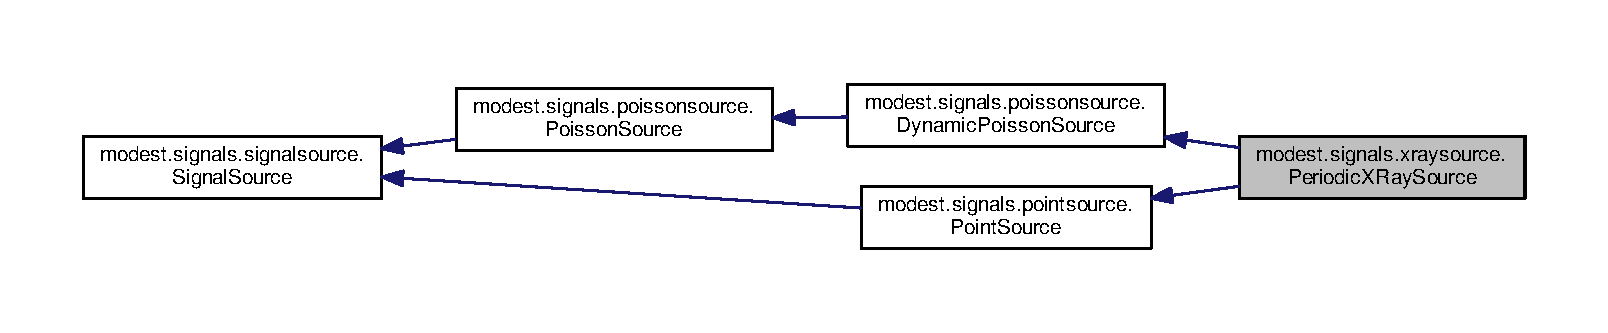
\includegraphics[width=350pt]{classmodest_1_1signals_1_1xraysource_1_1PeriodicXRaySource__inherit__graph}
\end{center}
\end{figure}


Collaboration diagram for modest.\+signals.\+xraysource.\+Periodic\+X\+Ray\+Source\+:\nopagebreak
\begin{figure}[H]
\begin{center}
\leavevmode
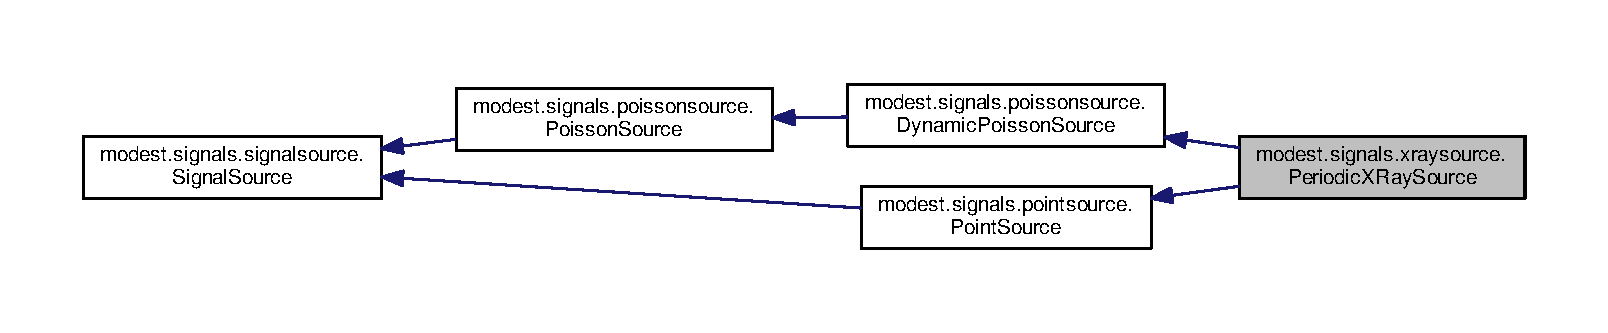
\includegraphics[width=350pt]{classmodest_1_1signals_1_1xraysource_1_1PeriodicXRaySource__coll__graph}
\end{center}
\end{figure}
\subsection*{Public Member Functions}
\begin{DoxyCompactItemize}
\item 
def \hyperlink{classmodest_1_1signals_1_1xraysource_1_1PeriodicXRaySource_af2583ad4d79406264881778edf1283fc}{\+\_\+\+\_\+init\+\_\+\+\_\+} (self, \hyperlink{classmodest_1_1signals_1_1xraysource_1_1PeriodicXRaySource_a50e061bb97d0dd6ab7f344370c6b35a4}{profile}, \hyperlink{classmodest_1_1signals_1_1xraysource_1_1PeriodicXRaySource_ac227ebef6424695360f2771765b4a4a7}{avg\+Photon\+Flux}=None, \hyperlink{classmodest_1_1signals_1_1xraysource_1_1PeriodicXRaySource_a5f968d9c80e5315d1657eac2ffca4e73}{pulsed\+Fraction}=None, P\+A\+R\+File=None, move\+Peak\+To\+Zero=True, \hyperlink{classmodest_1_1signals_1_1xraysource_1_1PeriodicXRaySource_ac7490bebcc1d508b7813ea274cc36702}{normalize\+Profile}=True, \hyperlink{classmodest_1_1signals_1_1xraysource_1_1PeriodicXRaySource_ad885c269b3b042b3d094412683ef3476}{phase\+Derivatives}=None, \hyperlink{classmodest_1_1signals_1_1xraysource_1_1PeriodicXRaySource_aeb6d4a8057d3ee58c81e69fb97b9eef7}{pulsar\+Period}=None, RA=None, D\+EC=None, \hyperlink{classmodest_1_1signals_1_1xraysource_1_1PeriodicXRaySource_aecd53533d34a4f821f4010c197edc2e8}{T\+Z\+R\+M\+JD}=None, \hyperlink{classmodest_1_1signals_1_1xraysource_1_1PeriodicXRaySource_aac8308319d4f31067e1087660a15db03}{name}=None, \hyperlink{classmodest_1_1signals_1_1pointsource_1_1PointSource_a0924a2233bb4fd23e50d024e4f1b048e}{attitude\+State\+Name}=\textquotesingle{}attitude\textquotesingle{}, \hyperlink{classmodest_1_1signals_1_1poissonsource_1_1DynamicPoissonSource_ac7f62303bb8a417a1ddefb032c707bcd}{correlation\+State\+Name}=None)
\item 
def \hyperlink{classmodest_1_1signals_1_1xraysource_1_1PeriodicXRaySource_a50045a93644e23cbaa88a4b4458694e2}{process\+Profile} (self, \hyperlink{classmodest_1_1signals_1_1xraysource_1_1PeriodicXRaySource_a50e061bb97d0dd6ab7f344370c6b35a4}{profile}, \hyperlink{classmodest_1_1signals_1_1xraysource_1_1PeriodicXRaySource_ac7490bebcc1d508b7813ea274cc36702}{normalize\+Profile}=True, move\+Peak\+To\+Zero=True)
\item 
def \hyperlink{classmodest_1_1signals_1_1xraysource_1_1PeriodicXRaySource_a98ef4d72f127017fab68dcdeab0dad64}{process\+P\+A\+R\+File} (self, P\+A\+R\+File, replace\+Current\+Values=False)
\item 
def \hyperlink{classmodest_1_1signals_1_1xraysource_1_1PeriodicXRaySource_a20315b15ec1f6141e35a029b5cabf717}{compute\+Single\+Period\+Integral} (self)
\item 
def \hyperlink{classmodest_1_1signals_1_1xraysource_1_1PeriodicXRaySource_a3ea2f37c1387cc682819e667a8ce7f1e}{get\+Phase} (self, observatory\+Time)
\item 
def \hyperlink{classmodest_1_1signals_1_1xraysource_1_1PeriodicXRaySource_a9949b9a2d7a2ed0e4bb731e3e4fb7d2f}{get\+Signal\+M\+JD} (self, M\+JD)
\begin{DoxyCompactList}\small\item\em \hyperlink{classmodest_1_1signals_1_1xraysource_1_1PeriodicXRaySource_a9949b9a2d7a2ed0e4bb731e3e4fb7d2f}{get\+Signal\+M\+JD} is a wrapper function that returns the photon flux at a given Modified Julian Date \end{DoxyCompactList}\item 
def \hyperlink{classmodest_1_1signals_1_1xraysource_1_1PeriodicXRaySource_ac446c2e2083dbd59865c96c34dd6623f}{get\+Signal} (self, observatory\+Time, t\+Var=None, state=None)
\begin{DoxyCompactList}\small\item\em \hyperlink{classmodest_1_1signals_1_1xraysource_1_1PeriodicXRaySource_ac446c2e2083dbd59865c96c34dd6623f}{get\+Signal} is responsible for returning the photon flux from the pulsar at a given time \end{DoxyCompactList}\item 
def \hyperlink{classmodest_1_1signals_1_1xraysource_1_1PeriodicXRaySource_a252850e9966b3281a193c834cb687646}{get\+Pulse\+From\+Phase} (self, phase)
\item 
def \hyperlink{classmodest_1_1signals_1_1xraysource_1_1PeriodicXRaySource_abdd0337b42d16288c8ad3dede15a99f2}{M\+J\+D2seconds} (self, M\+JD)
\item 
def \hyperlink{classmodest_1_1signals_1_1xraysource_1_1PeriodicXRaySource_a023967f167c21ca3a6020eb36dd7a7d7}{seconds2\+M\+JD} (self, seconds)
\item 
def \hyperlink{classmodest_1_1signals_1_1xraysource_1_1PeriodicXRaySource_ae9e8cdc926982f0cfbf038b6857a5c83}{compute\+Association\+Probability} (self, measurement, state\+Dict, validation\+Threshold=0)
\item 
def \hyperlink{classmodest_1_1signals_1_1xraysource_1_1PeriodicXRaySource_a640937825e6219bc7cc27168ed0e7fb0}{plot} (self, n\+Periods=1, t\+Var=None, figure\+Handle=None)
\item 
def \hyperlink{classmodest_1_1signals_1_1poissonsource_1_1DynamicPoissonSource_a6c8820d8007c848d745f9313efdb970c}{compute\+Association\+Probability} (self, measurement, state\+Dict)
\item 
def \hyperlink{classmodest_1_1signals_1_1signalsource_1_1SignalSource_a9a64c6a9c2954f6ad61e4ca3518ea8ab}{signal\+ID} (self)
\item 
def \hyperlink{classmodest_1_1signals_1_1pointsource_1_1PointSource_a295eb1a487e18c77029585ac2785db80}{Ra\+Dec} (self)
\item 
def \hyperlink{classmodest_1_1signals_1_1pointsource_1_1PointSource_a133933430a784107258901e257778221}{unit\+Vec} (self, \hyperlink{classmodest_1_1signals_1_1pointsource_1_1PointSource_a295eb1a487e18c77029585ac2785db80}{Ra\+Dec}=None)
\item 
def \hyperlink{classmodest_1_1signals_1_1signalsource_1_1SignalSource_a9a64c6a9c2954f6ad61e4ca3518ea8ab}{signal\+ID} (self)
\end{DoxyCompactItemize}
\subsection*{Static Public Member Functions}
\begin{DoxyCompactItemize}
\item 
def \hyperlink{classmodest_1_1signals_1_1xraysource_1_1PeriodicXRaySource_ae9e07e0f728014ba3b6af0022d6367fe}{hms2rad} (h, m, s)
\item 
def \hyperlink{classmodest_1_1signals_1_1xraysource_1_1PeriodicXRaySource_a117b7c3ff21b26887d74fce01ffad0a8}{dms2rad} (d, m, s)
\end{DoxyCompactItemize}
\subsection*{Public Attributes}
\begin{DoxyCompactItemize}
\item 
\hyperlink{classmodest_1_1signals_1_1xraysource_1_1PeriodicXRaySource_ad885c269b3b042b3d094412683ef3476}{phase\+Derivatives}
\begin{DoxyCompactList}\small\item\em Stores the derivatives of phase with respect to time  \hyperlink{classmodest_1_1signals_1_1xraysource_1_1PeriodicXRaySource_ad885c269b3b042b3d094412683ef3476}{phase\+Derivatives} is a dict which contains the derivatives of phase with respect to time. \end{DoxyCompactList}\item 
\hyperlink{classmodest_1_1signals_1_1xraysource_1_1PeriodicXRaySource_aecd53533d34a4f821f4010c197edc2e8}{T\+Z\+R\+M\+JD}
\begin{DoxyCompactList}\small\item\em \hyperlink{classmodest_1_1signals_1_1xraysource_1_1PeriodicXRaySource_aecd53533d34a4f821f4010c197edc2e8}{T\+Z\+R\+M\+JD} stores the Modified Julian Date (M\+JD) corresponding to t=0 seconds. \end{DoxyCompactList}\item 
\hyperlink{classmodest_1_1signals_1_1xraysource_1_1PeriodicXRaySource_aac8308319d4f31067e1087660a15db03}{name}
\begin{DoxyCompactList}\small\item\em \hyperlink{classmodest_1_1signals_1_1xraysource_1_1PeriodicXRaySource_aac8308319d4f31067e1087660a15db03}{name} is an arbitrary string that is used to identify the signal. \end{DoxyCompactList}\item 
\hyperlink{classmodest_1_1signals_1_1xraysource_1_1PeriodicXRaySource_ac227ebef6424695360f2771765b4a4a7}{avg\+Photon\+Flux}
\begin{DoxyCompactList}\small\item\em \#average\+Photon\+Flux is the mean value of photons expected to arrive from the signal per second (units of photons/second) \end{DoxyCompactList}\item 
\hyperlink{classmodest_1_1signals_1_1xraysource_1_1PeriodicXRaySource_a5f968d9c80e5315d1657eac2ffca4e73}{pulsed\+Fraction}
\begin{DoxyCompactList}\small\item\em \hyperlink{classmodest_1_1signals_1_1xraysource_1_1PeriodicXRaySource_a5f968d9c80e5315d1657eac2ffca4e73}{pulsed\+Fraction} is a value from 0 to 1 which indicates what percentage of the \hyperlink{classmodest_1_1signals_1_1xraysource_1_1PeriodicXRaySource_ac227ebef6424695360f2771765b4a4a7}{avg\+Photon\+Flux} is \char`\"{}pulsed\char`\"{} and what percentage is constant/background \end{DoxyCompactList}\item 
\hyperlink{classmodest_1_1signals_1_1xraysource_1_1PeriodicXRaySource_ac7490bebcc1d508b7813ea274cc36702}{normalize\+Profile}
\begin{DoxyCompactList}\small\item\em \hyperlink{classmodest_1_1signals_1_1xraysource_1_1PeriodicXRaySource_ac7490bebcc1d508b7813ea274cc36702}{normalize\+Profile} is a boolean flag used to indicate whether the profile is normalized from zero to one. \end{DoxyCompactList}\item 
\hyperlink{classmodest_1_1signals_1_1xraysource_1_1PeriodicXRaySource_aeb6d4a8057d3ee58c81e69fb97b9eef7}{pulsar\+Period}
\begin{DoxyCompactList}\small\item\em \hyperlink{classmodest_1_1signals_1_1xraysource_1_1PeriodicXRaySource_aeb6d4a8057d3ee58c81e69fb97b9eef7}{pulsar\+Period} is the amouont of time (in seconds) for one complete pulsar pulse. \end{DoxyCompactList}\item 
\hyperlink{classmodest_1_1signals_1_1xraysource_1_1PeriodicXRaySource_a50e061bb97d0dd6ab7f344370c6b35a4}{profile}
\begin{DoxyCompactList}\small\item\em \hyperlink{classmodest_1_1signals_1_1xraysource_1_1PeriodicXRaySource_a50e061bb97d0dd6ab7f344370c6b35a4}{profile} is a numpy array containing the numerical value of flux over a single period of the signal. \end{DoxyCompactList}\item 
\hyperlink{classmodest_1_1signals_1_1xraysource_1_1PeriodicXRaySource_aaf45141c09e1fd35c80c49907fa44497}{profile\+Index}
\item 
\hyperlink{classmodest_1_1signals_1_1xraysource_1_1PeriodicXRaySource_ab193c1d52a5bd8b0798bf407abcca72d}{single\+Period\+Integral}
\item 
\hyperlink{classmodest_1_1signals_1_1xraysource_1_1PeriodicXRaySource_a9d4e5488915741b792df74c256782777}{profile\+Len}
\item 
\hyperlink{classmodest_1_1signals_1_1xraysource_1_1PeriodicXRaySource_a25ab09a55afd1da4f019ad580770e5f4}{photons\+Per\+Period}
\item 
\hyperlink{classmodest_1_1signals_1_1xraysource_1_1PeriodicXRaySource_ab9ca2f0588f7e2f23c5301e05070fe99}{peak\+Amplitude}
\item 
\hyperlink{classmodest_1_1signals_1_1xraysource_1_1PeriodicXRaySource_a1f4469f0818f93136c6c228bd6fb5a09}{scale\+Factor}
\item 
\hyperlink{classmodest_1_1signals_1_1xraysource_1_1PeriodicXRaySource_a3a04d3f0609b7454efc4ef9cdcd7b219}{background\+Count\+Rate}
\item 
\hyperlink{classmodest_1_1signals_1_1poissonsource_1_1DynamicPoissonSource_ac7f62303bb8a417a1ddefb032c707bcd}{correlation\+State\+Name}
\item 
\hyperlink{classmodest_1_1signals_1_1poissonsource_1_1PoissonSource_a34395fc83bd8743a0a5ee69f9392a606}{last\+Time}
\item 
\hyperlink{classmodest_1_1signals_1_1poissonsource_1_1PoissonSource_a6f2c657ad936b921715d826ac74f7fe5}{flux}
\item 
\hyperlink{classmodest_1_1signals_1_1pointsource_1_1PointSource_a0924a2233bb4fd23e50d024e4f1b048e}{attitude\+State\+Name}
\end{DoxyCompactItemize}
\subsection*{Static Public Attributes}
\begin{DoxyCompactItemize}
\item 
int \hyperlink{classmodest_1_1signals_1_1signalsource_1_1SignalSource_a453eafb550b551adbec0903deb63dfce}{next\+Signal\+ID} = 0
\item 
int \hyperlink{classmodest_1_1signals_1_1signalsource_1_1SignalSource_a453eafb550b551adbec0903deb63dfce}{next\+Signal\+ID} = 0
\end{DoxyCompactItemize}


\subsection{Detailed Description}


Definition at line 88 of file xraysource.\+py.



\subsection{Constructor \& Destructor Documentation}
\index{modest\+::signals\+::xraysource\+::\+Periodic\+X\+Ray\+Source@{modest\+::signals\+::xraysource\+::\+Periodic\+X\+Ray\+Source}!\+\_\+\+\_\+init\+\_\+\+\_\+@{\+\_\+\+\_\+init\+\_\+\+\_\+}}
\index{\+\_\+\+\_\+init\+\_\+\+\_\+@{\+\_\+\+\_\+init\+\_\+\+\_\+}!modest\+::signals\+::xraysource\+::\+Periodic\+X\+Ray\+Source@{modest\+::signals\+::xraysource\+::\+Periodic\+X\+Ray\+Source}}
\subsubsection[{\texorpdfstring{\+\_\+\+\_\+init\+\_\+\+\_\+(self, profile, avg\+Photon\+Flux=\+None, pulsed\+Fraction=\+None, P\+A\+R\+File=\+None, move\+Peak\+To\+Zero=\+True, normalize\+Profile=\+True, phase\+Derivatives=\+None, pulsar\+Period=\+None, R\+A=\+None, D\+E\+C=\+None, T\+Z\+R\+M\+J\+D=\+None, name=\+None, attitude\+State\+Name=\textquotesingle{}attitude\textquotesingle{}, correlation\+State\+Name=\+None)}{__init__(self, profile, avgPhotonFlux=None, pulsedFraction=None, PARFile=None, movePeakToZero=True, normalizeProfile=True, phaseDerivatives=None, pulsarPeriod=None, RA=None, DEC=None, TZRMJD=None, name=None, attitudeStateName='attitude', correlationStateName=None)}}]{\setlength{\rightskip}{0pt plus 5cm}def modest.\+signals.\+xraysource.\+Periodic\+X\+Ray\+Source.\+\_\+\+\_\+init\+\_\+\+\_\+ (
\begin{DoxyParamCaption}
\item[{}]{self, }
\item[{}]{profile, }
\item[{}]{avg\+Photon\+Flux = {\ttfamily None}, }
\item[{}]{pulsed\+Fraction = {\ttfamily None}, }
\item[{}]{P\+A\+R\+File = {\ttfamily None}, }
\item[{}]{move\+Peak\+To\+Zero = {\ttfamily True}, }
\item[{}]{normalize\+Profile = {\ttfamily True}, }
\item[{}]{phase\+Derivatives = {\ttfamily None}, }
\item[{}]{pulsar\+Period = {\ttfamily None}, }
\item[{}]{RA = {\ttfamily None}, }
\item[{}]{D\+EC = {\ttfamily None}, }
\item[{}]{T\+Z\+R\+M\+JD = {\ttfamily None}, }
\item[{}]{name = {\ttfamily None}, }
\item[{}]{attitude\+State\+Name = {\ttfamily \textquotesingle{}attitude\textquotesingle{}}, }
\item[{}]{correlation\+State\+Name = {\ttfamily None}}
\end{DoxyParamCaption}
)}\hypertarget{classmodest_1_1signals_1_1xraysource_1_1PeriodicXRaySource_af2583ad4d79406264881778edf1283fc}{}\label{classmodest_1_1signals_1_1xraysource_1_1PeriodicXRaySource_af2583ad4d79406264881778edf1283fc}


Definition at line 105 of file xraysource.\+py.



\subsection{Member Function Documentation}
\index{modest\+::signals\+::xraysource\+::\+Periodic\+X\+Ray\+Source@{modest\+::signals\+::xraysource\+::\+Periodic\+X\+Ray\+Source}!compute\+Association\+Probability@{compute\+Association\+Probability}}
\index{compute\+Association\+Probability@{compute\+Association\+Probability}!modest\+::signals\+::xraysource\+::\+Periodic\+X\+Ray\+Source@{modest\+::signals\+::xraysource\+::\+Periodic\+X\+Ray\+Source}}
\subsubsection[{\texorpdfstring{compute\+Association\+Probability(self, measurement, state\+Dict)}{computeAssociationProbability(self, measurement, stateDict)}}]{\setlength{\rightskip}{0pt plus 5cm}def modest.\+signals.\+poissonsource.\+Dynamic\+Poisson\+Source.\+compute\+Association\+Probability (
\begin{DoxyParamCaption}
\item[{}]{self, }
\item[{}]{measurement, }
\item[{}]{state\+Dict}
\end{DoxyParamCaption}
)\hspace{0.3cm}{\ttfamily [inherited]}}\hypertarget{classmodest_1_1signals_1_1poissonsource_1_1DynamicPoissonSource_a6c8820d8007c848d745f9313efdb970c}{}\label{classmodest_1_1signals_1_1poissonsource_1_1DynamicPoissonSource_a6c8820d8007c848d745f9313efdb970c}


Definition at line 74 of file poissonsource.\+py.

\index{modest\+::signals\+::xraysource\+::\+Periodic\+X\+Ray\+Source@{modest\+::signals\+::xraysource\+::\+Periodic\+X\+Ray\+Source}!compute\+Association\+Probability@{compute\+Association\+Probability}}
\index{compute\+Association\+Probability@{compute\+Association\+Probability}!modest\+::signals\+::xraysource\+::\+Periodic\+X\+Ray\+Source@{modest\+::signals\+::xraysource\+::\+Periodic\+X\+Ray\+Source}}
\subsubsection[{\texorpdfstring{compute\+Association\+Probability(self, measurement, state\+Dict, validation\+Threshold=0)}{computeAssociationProbability(self, measurement, stateDict, validationThreshold=0)}}]{\setlength{\rightskip}{0pt plus 5cm}def modest.\+signals.\+xraysource.\+Periodic\+X\+Ray\+Source.\+compute\+Association\+Probability (
\begin{DoxyParamCaption}
\item[{}]{self, }
\item[{}]{measurement, }
\item[{}]{state\+Dict, }
\item[{}]{validation\+Threshold = {\ttfamily 0}}
\end{DoxyParamCaption}
)}\hypertarget{classmodest_1_1signals_1_1xraysource_1_1PeriodicXRaySource_ae9e8cdc926982f0cfbf038b6857a5c83}{}\label{classmodest_1_1signals_1_1xraysource_1_1PeriodicXRaySource_ae9e8cdc926982f0cfbf038b6857a5c83}


Definition at line 549 of file xraysource.\+py.

\index{modest\+::signals\+::xraysource\+::\+Periodic\+X\+Ray\+Source@{modest\+::signals\+::xraysource\+::\+Periodic\+X\+Ray\+Source}!compute\+Single\+Period\+Integral@{compute\+Single\+Period\+Integral}}
\index{compute\+Single\+Period\+Integral@{compute\+Single\+Period\+Integral}!modest\+::signals\+::xraysource\+::\+Periodic\+X\+Ray\+Source@{modest\+::signals\+::xraysource\+::\+Periodic\+X\+Ray\+Source}}
\subsubsection[{\texorpdfstring{compute\+Single\+Period\+Integral(self)}{computeSinglePeriodIntegral(self)}}]{\setlength{\rightskip}{0pt plus 5cm}def modest.\+signals.\+xraysource.\+Periodic\+X\+Ray\+Source.\+compute\+Single\+Period\+Integral (
\begin{DoxyParamCaption}
\item[{}]{self}
\end{DoxyParamCaption}
)}\hypertarget{classmodest_1_1signals_1_1xraysource_1_1PeriodicXRaySource_a20315b15ec1f6141e35a029b5cabf717}{}\label{classmodest_1_1signals_1_1xraysource_1_1PeriodicXRaySource_a20315b15ec1f6141e35a029b5cabf717}


Definition at line 328 of file xraysource.\+py.

\index{modest\+::signals\+::xraysource\+::\+Periodic\+X\+Ray\+Source@{modest\+::signals\+::xraysource\+::\+Periodic\+X\+Ray\+Source}!dms2rad@{dms2rad}}
\index{dms2rad@{dms2rad}!modest\+::signals\+::xraysource\+::\+Periodic\+X\+Ray\+Source@{modest\+::signals\+::xraysource\+::\+Periodic\+X\+Ray\+Source}}
\subsubsection[{\texorpdfstring{dms2rad(d, m, s)}{dms2rad(d, m, s)}}]{\setlength{\rightskip}{0pt plus 5cm}def modest.\+signals.\+xraysource.\+Periodic\+X\+Ray\+Source.\+dms2rad (
\begin{DoxyParamCaption}
\item[{}]{d, }
\item[{}]{m, }
\item[{}]{s}
\end{DoxyParamCaption}
)\hspace{0.3cm}{\ttfamily [static]}}\hypertarget{classmodest_1_1signals_1_1xraysource_1_1PeriodicXRaySource_a117b7c3ff21b26887d74fce01ffad0a8}{}\label{classmodest_1_1signals_1_1xraysource_1_1PeriodicXRaySource_a117b7c3ff21b26887d74fce01ffad0a8}


Definition at line 593 of file xraysource.\+py.

\index{modest\+::signals\+::xraysource\+::\+Periodic\+X\+Ray\+Source@{modest\+::signals\+::xraysource\+::\+Periodic\+X\+Ray\+Source}!get\+Phase@{get\+Phase}}
\index{get\+Phase@{get\+Phase}!modest\+::signals\+::xraysource\+::\+Periodic\+X\+Ray\+Source@{modest\+::signals\+::xraysource\+::\+Periodic\+X\+Ray\+Source}}
\subsubsection[{\texorpdfstring{get\+Phase(self, observatory\+Time)}{getPhase(self, observatoryTime)}}]{\setlength{\rightskip}{0pt plus 5cm}def modest.\+signals.\+xraysource.\+Periodic\+X\+Ray\+Source.\+get\+Phase (
\begin{DoxyParamCaption}
\item[{}]{self, }
\item[{}]{observatory\+Time}
\end{DoxyParamCaption}
)}\hypertarget{classmodest_1_1signals_1_1xraysource_1_1PeriodicXRaySource_a3ea2f37c1387cc682819e667a8ce7f1e}{}\label{classmodest_1_1signals_1_1xraysource_1_1PeriodicXRaySource_a3ea2f37c1387cc682819e667a8ce7f1e}


Definition at line 387 of file xraysource.\+py.

\index{modest\+::signals\+::xraysource\+::\+Periodic\+X\+Ray\+Source@{modest\+::signals\+::xraysource\+::\+Periodic\+X\+Ray\+Source}!get\+Pulse\+From\+Phase@{get\+Pulse\+From\+Phase}}
\index{get\+Pulse\+From\+Phase@{get\+Pulse\+From\+Phase}!modest\+::signals\+::xraysource\+::\+Periodic\+X\+Ray\+Source@{modest\+::signals\+::xraysource\+::\+Periodic\+X\+Ray\+Source}}
\subsubsection[{\texorpdfstring{get\+Pulse\+From\+Phase(self, phase)}{getPulseFromPhase(self, phase)}}]{\setlength{\rightskip}{0pt plus 5cm}def modest.\+signals.\+xraysource.\+Periodic\+X\+Ray\+Source.\+get\+Pulse\+From\+Phase (
\begin{DoxyParamCaption}
\item[{}]{self, }
\item[{}]{phase}
\end{DoxyParamCaption}
)}\hypertarget{classmodest_1_1signals_1_1xraysource_1_1PeriodicXRaySource_a252850e9966b3281a193c834cb687646}{}\label{classmodest_1_1signals_1_1xraysource_1_1PeriodicXRaySource_a252850e9966b3281a193c834cb687646}


Definition at line 526 of file xraysource.\+py.

\index{modest\+::signals\+::xraysource\+::\+Periodic\+X\+Ray\+Source@{modest\+::signals\+::xraysource\+::\+Periodic\+X\+Ray\+Source}!get\+Signal@{get\+Signal}}
\index{get\+Signal@{get\+Signal}!modest\+::signals\+::xraysource\+::\+Periodic\+X\+Ray\+Source@{modest\+::signals\+::xraysource\+::\+Periodic\+X\+Ray\+Source}}
\subsubsection[{\texorpdfstring{get\+Signal(self, observatory\+Time, t\+Var=\+None, state=\+None)}{getSignal(self, observatoryTime, tVar=None, state=None)}}]{\setlength{\rightskip}{0pt plus 5cm}def modest.\+signals.\+xraysource.\+Periodic\+X\+Ray\+Source.\+get\+Signal (
\begin{DoxyParamCaption}
\item[{}]{self, }
\item[{}]{observatory\+Time, }
\item[{}]{t\+Var = {\ttfamily None}, }
\item[{}]{state = {\ttfamily None}}
\end{DoxyParamCaption}
)}\hypertarget{classmodest_1_1signals_1_1xraysource_1_1PeriodicXRaySource_ac446c2e2083dbd59865c96c34dd6623f}{}\label{classmodest_1_1signals_1_1xraysource_1_1PeriodicXRaySource_ac446c2e2083dbd59865c96c34dd6623f}


\hyperlink{classmodest_1_1signals_1_1xraysource_1_1PeriodicXRaySource_ac446c2e2083dbd59865c96c34dd6623f}{get\+Signal} is responsible for returning the photon flux from the pulsar at a given time 

The \hyperlink{classmodest_1_1signals_1_1xraysource_1_1PeriodicXRaySource_ac446c2e2083dbd59865c96c34dd6623f}{get\+Signal} method is the method which is responsible for returning the current value of flux from the signal source at a given time. If there is uncertainty in the time, then the expected value of the signal is returned. Uncertainty in time is indicated by the optional t\+Var argument.

In every case, the method calls the \hyperlink{classmodest_1_1signals_1_1xraysource_1_1PeriodicXRaySource_a3ea2f37c1387cc682819e667a8ce7f1e}{get\+Phase} method to determine the current signal source phase. If no uncertainty in time is passed, then the \hyperlink{classmodest_1_1signals_1_1xraysource_1_1PeriodicXRaySource_a252850e9966b3281a193c834cb687646}{get\+Pulse\+From\+Phase} method is called to lookup/interpolate the current flux based on the phase and the signal \hyperlink{classmodest_1_1signals_1_1xraysource_1_1PeriodicXRaySource_a50e061bb97d0dd6ab7f344370c6b35a4}{profile}.

If a value is passed for t\+Var, then the process is more complicated. Rather than simply look up the signal value from the phase, the function returns an approximation of the expected value of the signal, given the mean and variance of time.

Normally, the expected value would be computed by integrating the product of the true distribution of time (probably a normal distribution) with the flux as a function of time. However, due to the non-\/analytical nature of the flux function, the direct computation of this integral is intractable. To overcome this limitation, the time distributuion is approximated as a moment-\/matched uniform distribution. Using this approximation, the approximate integral may be directly computed simply by looking up the start and end values of \hyperlink{classmodest_1_1signals_1_1xraysource_1_1PeriodicXRaySource_ab193c1d52a5bd8b0798bf407abcca72d}{single\+Period\+Integral}, and dividing by the appropriate scaling factor.


\begin{DoxyParams}{Parameters}
{\em self} & The object pointer \\
\hline
{\em observatory\+Time} & The time for which to compute the signal \\
\hline
{\em t\+Var} & (optional) The variance of the time estimate\\
\hline
\end{DoxyParams}
\begin{DoxyReturn}{Returns}
The signal at the requested time 
\end{DoxyReturn}


Definition at line 454 of file xraysource.\+py.

\index{modest\+::signals\+::xraysource\+::\+Periodic\+X\+Ray\+Source@{modest\+::signals\+::xraysource\+::\+Periodic\+X\+Ray\+Source}!get\+Signal\+M\+JD@{get\+Signal\+M\+JD}}
\index{get\+Signal\+M\+JD@{get\+Signal\+M\+JD}!modest\+::signals\+::xraysource\+::\+Periodic\+X\+Ray\+Source@{modest\+::signals\+::xraysource\+::\+Periodic\+X\+Ray\+Source}}
\subsubsection[{\texorpdfstring{get\+Signal\+M\+J\+D(self, M\+J\+D)}{getSignalMJD(self, MJD)}}]{\setlength{\rightskip}{0pt plus 5cm}def modest.\+signals.\+xraysource.\+Periodic\+X\+Ray\+Source.\+get\+Signal\+M\+JD (
\begin{DoxyParamCaption}
\item[{}]{self, }
\item[{}]{M\+JD}
\end{DoxyParamCaption}
)}\hypertarget{classmodest_1_1signals_1_1xraysource_1_1PeriodicXRaySource_a9949b9a2d7a2ed0e4bb731e3e4fb7d2f}{}\label{classmodest_1_1signals_1_1xraysource_1_1PeriodicXRaySource_a9949b9a2d7a2ed0e4bb731e3e4fb7d2f}


\hyperlink{classmodest_1_1signals_1_1xraysource_1_1PeriodicXRaySource_a9949b9a2d7a2ed0e4bb731e3e4fb7d2f}{get\+Signal\+M\+JD} is a wrapper function that returns the photon flux at a given Modified Julian Date 


\begin{DoxyParams}{Parameters}
{\em self} & The object pointer \\
\hline
{\em M\+JD} & The Modified Jullian Date for which flux is to be returned\\
\hline
\end{DoxyParams}
\begin{DoxyReturn}{Returns}
The signal at the requested date 
\end{DoxyReturn}


Definition at line 410 of file xraysource.\+py.

\index{modest\+::signals\+::xraysource\+::\+Periodic\+X\+Ray\+Source@{modest\+::signals\+::xraysource\+::\+Periodic\+X\+Ray\+Source}!hms2rad@{hms2rad}}
\index{hms2rad@{hms2rad}!modest\+::signals\+::xraysource\+::\+Periodic\+X\+Ray\+Source@{modest\+::signals\+::xraysource\+::\+Periodic\+X\+Ray\+Source}}
\subsubsection[{\texorpdfstring{hms2rad(h, m, s)}{hms2rad(h, m, s)}}]{\setlength{\rightskip}{0pt plus 5cm}def modest.\+signals.\+xraysource.\+Periodic\+X\+Ray\+Source.\+hms2rad (
\begin{DoxyParamCaption}
\item[{}]{h, }
\item[{}]{m, }
\item[{}]{s}
\end{DoxyParamCaption}
)\hspace{0.3cm}{\ttfamily [static]}}\hypertarget{classmodest_1_1signals_1_1xraysource_1_1PeriodicXRaySource_ae9e07e0f728014ba3b6af0022d6367fe}{}\label{classmodest_1_1signals_1_1xraysource_1_1PeriodicXRaySource_ae9e07e0f728014ba3b6af0022d6367fe}


Definition at line 587 of file xraysource.\+py.

\index{modest\+::signals\+::xraysource\+::\+Periodic\+X\+Ray\+Source@{modest\+::signals\+::xraysource\+::\+Periodic\+X\+Ray\+Source}!M\+J\+D2seconds@{M\+J\+D2seconds}}
\index{M\+J\+D2seconds@{M\+J\+D2seconds}!modest\+::signals\+::xraysource\+::\+Periodic\+X\+Ray\+Source@{modest\+::signals\+::xraysource\+::\+Periodic\+X\+Ray\+Source}}
\subsubsection[{\texorpdfstring{M\+J\+D2seconds(self, M\+J\+D)}{MJD2seconds(self, MJD)}}]{\setlength{\rightskip}{0pt plus 5cm}def modest.\+signals.\+xraysource.\+Periodic\+X\+Ray\+Source.\+M\+J\+D2seconds (
\begin{DoxyParamCaption}
\item[{}]{self, }
\item[{}]{M\+JD}
\end{DoxyParamCaption}
)}\hypertarget{classmodest_1_1signals_1_1xraysource_1_1PeriodicXRaySource_abdd0337b42d16288c8ad3dede15a99f2}{}\label{classmodest_1_1signals_1_1xraysource_1_1PeriodicXRaySource_abdd0337b42d16288c8ad3dede15a99f2}


Definition at line 535 of file xraysource.\+py.

\index{modest\+::signals\+::xraysource\+::\+Periodic\+X\+Ray\+Source@{modest\+::signals\+::xraysource\+::\+Periodic\+X\+Ray\+Source}!plot@{plot}}
\index{plot@{plot}!modest\+::signals\+::xraysource\+::\+Periodic\+X\+Ray\+Source@{modest\+::signals\+::xraysource\+::\+Periodic\+X\+Ray\+Source}}
\subsubsection[{\texorpdfstring{plot(self, n\+Periods=1, t\+Var=\+None, figure\+Handle=\+None)}{plot(self, nPeriods=1, tVar=None, figureHandle=None)}}]{\setlength{\rightskip}{0pt plus 5cm}def modest.\+signals.\+xraysource.\+Periodic\+X\+Ray\+Source.\+plot (
\begin{DoxyParamCaption}
\item[{}]{self, }
\item[{}]{n\+Periods = {\ttfamily 1}, }
\item[{}]{t\+Var = {\ttfamily None}, }
\item[{}]{figure\+Handle = {\ttfamily None}}
\end{DoxyParamCaption}
)}\hypertarget{classmodest_1_1signals_1_1xraysource_1_1PeriodicXRaySource_a640937825e6219bc7cc27168ed0e7fb0}{}\label{classmodest_1_1signals_1_1xraysource_1_1PeriodicXRaySource_a640937825e6219bc7cc27168ed0e7fb0}


Definition at line 569 of file xraysource.\+py.

\index{modest\+::signals\+::xraysource\+::\+Periodic\+X\+Ray\+Source@{modest\+::signals\+::xraysource\+::\+Periodic\+X\+Ray\+Source}!process\+P\+A\+R\+File@{process\+P\+A\+R\+File}}
\index{process\+P\+A\+R\+File@{process\+P\+A\+R\+File}!modest\+::signals\+::xraysource\+::\+Periodic\+X\+Ray\+Source@{modest\+::signals\+::xraysource\+::\+Periodic\+X\+Ray\+Source}}
\subsubsection[{\texorpdfstring{process\+P\+A\+R\+File(self, P\+A\+R\+File, replace\+Current\+Values=\+False)}{processPARFile(self, PARFile, replaceCurrentValues=False)}}]{\setlength{\rightskip}{0pt plus 5cm}def modest.\+signals.\+xraysource.\+Periodic\+X\+Ray\+Source.\+process\+P\+A\+R\+File (
\begin{DoxyParamCaption}
\item[{}]{self, }
\item[{}]{P\+A\+R\+File, }
\item[{}]{replace\+Current\+Values = {\ttfamily False}}
\end{DoxyParamCaption}
)}\hypertarget{classmodest_1_1signals_1_1xraysource_1_1PeriodicXRaySource_a98ef4d72f127017fab68dcdeab0dad64}{}\label{classmodest_1_1signals_1_1xraysource_1_1PeriodicXRaySource_a98ef4d72f127017fab68dcdeab0dad64}


Definition at line 248 of file xraysource.\+py.

\index{modest\+::signals\+::xraysource\+::\+Periodic\+X\+Ray\+Source@{modest\+::signals\+::xraysource\+::\+Periodic\+X\+Ray\+Source}!process\+Profile@{process\+Profile}}
\index{process\+Profile@{process\+Profile}!modest\+::signals\+::xraysource\+::\+Periodic\+X\+Ray\+Source@{modest\+::signals\+::xraysource\+::\+Periodic\+X\+Ray\+Source}}
\subsubsection[{\texorpdfstring{process\+Profile(self, profile, normalize\+Profile=\+True, move\+Peak\+To\+Zero=\+True)}{processProfile(self, profile, normalizeProfile=True, movePeakToZero=True)}}]{\setlength{\rightskip}{0pt plus 5cm}def modest.\+signals.\+xraysource.\+Periodic\+X\+Ray\+Source.\+process\+Profile (
\begin{DoxyParamCaption}
\item[{}]{self, }
\item[{}]{profile, }
\item[{}]{normalize\+Profile = {\ttfamily True}, }
\item[{}]{move\+Peak\+To\+Zero = {\ttfamily True}}
\end{DoxyParamCaption}
)}\hypertarget{classmodest_1_1signals_1_1xraysource_1_1PeriodicXRaySource_a50045a93644e23cbaa88a4b4458694e2}{}\label{classmodest_1_1signals_1_1xraysource_1_1PeriodicXRaySource_a50045a93644e23cbaa88a4b4458694e2}


Definition at line 206 of file xraysource.\+py.

\index{modest\+::signals\+::xraysource\+::\+Periodic\+X\+Ray\+Source@{modest\+::signals\+::xraysource\+::\+Periodic\+X\+Ray\+Source}!Ra\+Dec@{Ra\+Dec}}
\index{Ra\+Dec@{Ra\+Dec}!modest\+::signals\+::xraysource\+::\+Periodic\+X\+Ray\+Source@{modest\+::signals\+::xraysource\+::\+Periodic\+X\+Ray\+Source}}
\subsubsection[{\texorpdfstring{Ra\+Dec(self)}{RaDec(self)}}]{\setlength{\rightskip}{0pt plus 5cm}def modest.\+signals.\+pointsource.\+Point\+Source.\+Ra\+Dec (
\begin{DoxyParamCaption}
\item[{}]{self}
\end{DoxyParamCaption}
)\hspace{0.3cm}{\ttfamily [inherited]}}\hypertarget{classmodest_1_1signals_1_1pointsource_1_1PointSource_a295eb1a487e18c77029585ac2785db80}{}\label{classmodest_1_1signals_1_1pointsource_1_1PointSource_a295eb1a487e18c77029585ac2785db80}


Definition at line 21 of file pointsource.\+py.

\index{modest\+::signals\+::xraysource\+::\+Periodic\+X\+Ray\+Source@{modest\+::signals\+::xraysource\+::\+Periodic\+X\+Ray\+Source}!seconds2\+M\+JD@{seconds2\+M\+JD}}
\index{seconds2\+M\+JD@{seconds2\+M\+JD}!modest\+::signals\+::xraysource\+::\+Periodic\+X\+Ray\+Source@{modest\+::signals\+::xraysource\+::\+Periodic\+X\+Ray\+Source}}
\subsubsection[{\texorpdfstring{seconds2\+M\+J\+D(self, seconds)}{seconds2MJD(self, seconds)}}]{\setlength{\rightskip}{0pt plus 5cm}def modest.\+signals.\+xraysource.\+Periodic\+X\+Ray\+Source.\+seconds2\+M\+JD (
\begin{DoxyParamCaption}
\item[{}]{self, }
\item[{}]{seconds}
\end{DoxyParamCaption}
)}\hypertarget{classmodest_1_1signals_1_1xraysource_1_1PeriodicXRaySource_a023967f167c21ca3a6020eb36dd7a7d7}{}\label{classmodest_1_1signals_1_1xraysource_1_1PeriodicXRaySource_a023967f167c21ca3a6020eb36dd7a7d7}


Definition at line 541 of file xraysource.\+py.

\index{modest\+::signals\+::xraysource\+::\+Periodic\+X\+Ray\+Source@{modest\+::signals\+::xraysource\+::\+Periodic\+X\+Ray\+Source}!signal\+ID@{signal\+ID}}
\index{signal\+ID@{signal\+ID}!modest\+::signals\+::xraysource\+::\+Periodic\+X\+Ray\+Source@{modest\+::signals\+::xraysource\+::\+Periodic\+X\+Ray\+Source}}
\subsubsection[{\texorpdfstring{signal\+I\+D(self)}{signalID(self)}}]{\setlength{\rightskip}{0pt plus 5cm}def modest.\+signals.\+signalsource.\+Signal\+Source.\+signal\+ID (
\begin{DoxyParamCaption}
\item[{}]{self}
\end{DoxyParamCaption}
)\hspace{0.3cm}{\ttfamily [inherited]}}\hypertarget{classmodest_1_1signals_1_1signalsource_1_1SignalSource_a9a64c6a9c2954f6ad61e4ca3518ea8ab}{}\label{classmodest_1_1signals_1_1signalsource_1_1SignalSource_a9a64c6a9c2954f6ad61e4ca3518ea8ab}


Definition at line 17 of file signalsource.\+py.

\index{modest\+::signals\+::xraysource\+::\+Periodic\+X\+Ray\+Source@{modest\+::signals\+::xraysource\+::\+Periodic\+X\+Ray\+Source}!signal\+ID@{signal\+ID}}
\index{signal\+ID@{signal\+ID}!modest\+::signals\+::xraysource\+::\+Periodic\+X\+Ray\+Source@{modest\+::signals\+::xraysource\+::\+Periodic\+X\+Ray\+Source}}
\subsubsection[{\texorpdfstring{signal\+I\+D(self)}{signalID(self)}}]{\setlength{\rightskip}{0pt plus 5cm}def modest.\+signals.\+signalsource.\+Signal\+Source.\+signal\+ID (
\begin{DoxyParamCaption}
\item[{}]{self}
\end{DoxyParamCaption}
)\hspace{0.3cm}{\ttfamily [inherited]}}\hypertarget{classmodest_1_1signals_1_1signalsource_1_1SignalSource_a9a64c6a9c2954f6ad61e4ca3518ea8ab}{}\label{classmodest_1_1signals_1_1signalsource_1_1SignalSource_a9a64c6a9c2954f6ad61e4ca3518ea8ab}


Definition at line 17 of file signalsource.\+py.

\index{modest\+::signals\+::xraysource\+::\+Periodic\+X\+Ray\+Source@{modest\+::signals\+::xraysource\+::\+Periodic\+X\+Ray\+Source}!unit\+Vec@{unit\+Vec}}
\index{unit\+Vec@{unit\+Vec}!modest\+::signals\+::xraysource\+::\+Periodic\+X\+Ray\+Source@{modest\+::signals\+::xraysource\+::\+Periodic\+X\+Ray\+Source}}
\subsubsection[{\texorpdfstring{unit\+Vec(self, Ra\+Dec=\+None)}{unitVec(self, RaDec=None)}}]{\setlength{\rightskip}{0pt plus 5cm}def modest.\+signals.\+pointsource.\+Point\+Source.\+unit\+Vec (
\begin{DoxyParamCaption}
\item[{}]{self, }
\item[{}]{Ra\+Dec = {\ttfamily None}}
\end{DoxyParamCaption}
)\hspace{0.3cm}{\ttfamily [inherited]}}\hypertarget{classmodest_1_1signals_1_1pointsource_1_1PointSource_a133933430a784107258901e257778221}{}\label{classmodest_1_1signals_1_1pointsource_1_1PointSource_a133933430a784107258901e257778221}


Definition at line 26 of file pointsource.\+py.



\subsection{Member Data Documentation}
\index{modest\+::signals\+::xraysource\+::\+Periodic\+X\+Ray\+Source@{modest\+::signals\+::xraysource\+::\+Periodic\+X\+Ray\+Source}!attitude\+State\+Name@{attitude\+State\+Name}}
\index{attitude\+State\+Name@{attitude\+State\+Name}!modest\+::signals\+::xraysource\+::\+Periodic\+X\+Ray\+Source@{modest\+::signals\+::xraysource\+::\+Periodic\+X\+Ray\+Source}}
\subsubsection[{\texorpdfstring{attitude\+State\+Name}{attitudeStateName}}]{\setlength{\rightskip}{0pt plus 5cm}modest.\+signals.\+pointsource.\+Point\+Source.\+attitude\+State\+Name\hspace{0.3cm}{\ttfamily [inherited]}}\hypertarget{classmodest_1_1signals_1_1pointsource_1_1PointSource_a0924a2233bb4fd23e50d024e4f1b048e}{}\label{classmodest_1_1signals_1_1pointsource_1_1PointSource_a0924a2233bb4fd23e50d024e4f1b048e}


Definition at line 17 of file pointsource.\+py.

\index{modest\+::signals\+::xraysource\+::\+Periodic\+X\+Ray\+Source@{modest\+::signals\+::xraysource\+::\+Periodic\+X\+Ray\+Source}!avg\+Photon\+Flux@{avg\+Photon\+Flux}}
\index{avg\+Photon\+Flux@{avg\+Photon\+Flux}!modest\+::signals\+::xraysource\+::\+Periodic\+X\+Ray\+Source@{modest\+::signals\+::xraysource\+::\+Periodic\+X\+Ray\+Source}}
\subsubsection[{\texorpdfstring{avg\+Photon\+Flux}{avgPhotonFlux}}]{\setlength{\rightskip}{0pt plus 5cm}modest.\+signals.\+xraysource.\+Periodic\+X\+Ray\+Source.\+avg\+Photon\+Flux}\hypertarget{classmodest_1_1signals_1_1xraysource_1_1PeriodicXRaySource_ac227ebef6424695360f2771765b4a4a7}{}\label{classmodest_1_1signals_1_1xraysource_1_1PeriodicXRaySource_ac227ebef6424695360f2771765b4a4a7}


\#average\+Photon\+Flux is the mean value of photons expected to arrive from the signal per second (units of photons/second) 



Definition at line 138 of file xraysource.\+py.

\index{modest\+::signals\+::xraysource\+::\+Periodic\+X\+Ray\+Source@{modest\+::signals\+::xraysource\+::\+Periodic\+X\+Ray\+Source}!background\+Count\+Rate@{background\+Count\+Rate}}
\index{background\+Count\+Rate@{background\+Count\+Rate}!modest\+::signals\+::xraysource\+::\+Periodic\+X\+Ray\+Source@{modest\+::signals\+::xraysource\+::\+Periodic\+X\+Ray\+Source}}
\subsubsection[{\texorpdfstring{background\+Count\+Rate}{backgroundCountRate}}]{\setlength{\rightskip}{0pt plus 5cm}modest.\+signals.\+xraysource.\+Periodic\+X\+Ray\+Source.\+background\+Count\+Rate}\hypertarget{classmodest_1_1signals_1_1xraysource_1_1PeriodicXRaySource_a3a04d3f0609b7454efc4ef9cdcd7b219}{}\label{classmodest_1_1signals_1_1xraysource_1_1PeriodicXRaySource_a3a04d3f0609b7454efc4ef9cdcd7b219}


Definition at line 369 of file xraysource.\+py.

\index{modest\+::signals\+::xraysource\+::\+Periodic\+X\+Ray\+Source@{modest\+::signals\+::xraysource\+::\+Periodic\+X\+Ray\+Source}!correlation\+State\+Name@{correlation\+State\+Name}}
\index{correlation\+State\+Name@{correlation\+State\+Name}!modest\+::signals\+::xraysource\+::\+Periodic\+X\+Ray\+Source@{modest\+::signals\+::xraysource\+::\+Periodic\+X\+Ray\+Source}}
\subsubsection[{\texorpdfstring{correlation\+State\+Name}{correlationStateName}}]{\setlength{\rightskip}{0pt plus 5cm}modest.\+signals.\+poissonsource.\+Dynamic\+Poisson\+Source.\+correlation\+State\+Name\hspace{0.3cm}{\ttfamily [inherited]}}\hypertarget{classmodest_1_1signals_1_1poissonsource_1_1DynamicPoissonSource_ac7f62303bb8a417a1ddefb032c707bcd}{}\label{classmodest_1_1signals_1_1poissonsource_1_1DynamicPoissonSource_ac7f62303bb8a417a1ddefb032c707bcd}


Definition at line 54 of file poissonsource.\+py.

\index{modest\+::signals\+::xraysource\+::\+Periodic\+X\+Ray\+Source@{modest\+::signals\+::xraysource\+::\+Periodic\+X\+Ray\+Source}!flux@{flux}}
\index{flux@{flux}!modest\+::signals\+::xraysource\+::\+Periodic\+X\+Ray\+Source@{modest\+::signals\+::xraysource\+::\+Periodic\+X\+Ray\+Source}}
\subsubsection[{\texorpdfstring{flux}{flux}}]{\setlength{\rightskip}{0pt plus 5cm}modest.\+signals.\+poissonsource.\+Poisson\+Source.\+flux\hspace{0.3cm}{\ttfamily [inherited]}}\hypertarget{classmodest_1_1signals_1_1poissonsource_1_1PoissonSource_a6f2c657ad936b921715d826ac74f7fe5}{}\label{classmodest_1_1signals_1_1poissonsource_1_1PoissonSource_a6f2c657ad936b921715d826ac74f7fe5}


Definition at line 14 of file poissonsource.\+py.

\index{modest\+::signals\+::xraysource\+::\+Periodic\+X\+Ray\+Source@{modest\+::signals\+::xraysource\+::\+Periodic\+X\+Ray\+Source}!last\+Time@{last\+Time}}
\index{last\+Time@{last\+Time}!modest\+::signals\+::xraysource\+::\+Periodic\+X\+Ray\+Source@{modest\+::signals\+::xraysource\+::\+Periodic\+X\+Ray\+Source}}
\subsubsection[{\texorpdfstring{last\+Time}{lastTime}}]{\setlength{\rightskip}{0pt plus 5cm}modest.\+signals.\+poissonsource.\+Poisson\+Source.\+last\+Time\hspace{0.3cm}{\ttfamily [inherited]}}\hypertarget{classmodest_1_1signals_1_1poissonsource_1_1PoissonSource_a34395fc83bd8743a0a5ee69f9392a606}{}\label{classmodest_1_1signals_1_1poissonsource_1_1PoissonSource_a34395fc83bd8743a0a5ee69f9392a606}


Definition at line 13 of file poissonsource.\+py.

\index{modest\+::signals\+::xraysource\+::\+Periodic\+X\+Ray\+Source@{modest\+::signals\+::xraysource\+::\+Periodic\+X\+Ray\+Source}!name@{name}}
\index{name@{name}!modest\+::signals\+::xraysource\+::\+Periodic\+X\+Ray\+Source@{modest\+::signals\+::xraysource\+::\+Periodic\+X\+Ray\+Source}}
\subsubsection[{\texorpdfstring{name}{name}}]{\setlength{\rightskip}{0pt plus 5cm}modest.\+signals.\+xraysource.\+Periodic\+X\+Ray\+Source.\+name}\hypertarget{classmodest_1_1signals_1_1xraysource_1_1PeriodicXRaySource_aac8308319d4f31067e1087660a15db03}{}\label{classmodest_1_1signals_1_1xraysource_1_1PeriodicXRaySource_aac8308319d4f31067e1087660a15db03}


\hyperlink{classmodest_1_1signals_1_1xraysource_1_1PeriodicXRaySource_aac8308319d4f31067e1087660a15db03}{name} is an arbitrary string that is used to identify the signal. 

Can be set to whatever the user wants, since it is only used for display purposes. Usually set to the astrophysical signal\textquotesingle{}s name (i.\+e. \char`\"{}\+Crab Pulsar\char`\"{} or \char`\"{}\+P\+S\+R B0531+21\char`\"{}) 

Definition at line 134 of file xraysource.\+py.

\index{modest\+::signals\+::xraysource\+::\+Periodic\+X\+Ray\+Source@{modest\+::signals\+::xraysource\+::\+Periodic\+X\+Ray\+Source}!next\+Signal\+ID@{next\+Signal\+ID}}
\index{next\+Signal\+ID@{next\+Signal\+ID}!modest\+::signals\+::xraysource\+::\+Periodic\+X\+Ray\+Source@{modest\+::signals\+::xraysource\+::\+Periodic\+X\+Ray\+Source}}
\subsubsection[{\texorpdfstring{next\+Signal\+ID}{nextSignalID}}]{\setlength{\rightskip}{0pt plus 5cm}int modest.\+signals.\+signalsource.\+Signal\+Source.\+next\+Signal\+ID = 0\hspace{0.3cm}{\ttfamily [static]}, {\ttfamily [inherited]}}\hypertarget{classmodest_1_1signals_1_1signalsource_1_1SignalSource_a453eafb550b551adbec0903deb63dfce}{}\label{classmodest_1_1signals_1_1signalsource_1_1SignalSource_a453eafb550b551adbec0903deb63dfce}


Definition at line 8 of file signalsource.\+py.

\index{modest\+::signals\+::xraysource\+::\+Periodic\+X\+Ray\+Source@{modest\+::signals\+::xraysource\+::\+Periodic\+X\+Ray\+Source}!next\+Signal\+ID@{next\+Signal\+ID}}
\index{next\+Signal\+ID@{next\+Signal\+ID}!modest\+::signals\+::xraysource\+::\+Periodic\+X\+Ray\+Source@{modest\+::signals\+::xraysource\+::\+Periodic\+X\+Ray\+Source}}
\subsubsection[{\texorpdfstring{next\+Signal\+ID}{nextSignalID}}]{\setlength{\rightskip}{0pt plus 5cm}int modest.\+signals.\+signalsource.\+Signal\+Source.\+next\+Signal\+ID = 0\hspace{0.3cm}{\ttfamily [static]}, {\ttfamily [inherited]}}\hypertarget{classmodest_1_1signals_1_1signalsource_1_1SignalSource_a453eafb550b551adbec0903deb63dfce}{}\label{classmodest_1_1signals_1_1signalsource_1_1SignalSource_a453eafb550b551adbec0903deb63dfce}


Definition at line 8 of file signalsource.\+py.

\index{modest\+::signals\+::xraysource\+::\+Periodic\+X\+Ray\+Source@{modest\+::signals\+::xraysource\+::\+Periodic\+X\+Ray\+Source}!normalize\+Profile@{normalize\+Profile}}
\index{normalize\+Profile@{normalize\+Profile}!modest\+::signals\+::xraysource\+::\+Periodic\+X\+Ray\+Source@{modest\+::signals\+::xraysource\+::\+Periodic\+X\+Ray\+Source}}
\subsubsection[{\texorpdfstring{normalize\+Profile}{normalizeProfile}}]{\setlength{\rightskip}{0pt plus 5cm}modest.\+signals.\+xraysource.\+Periodic\+X\+Ray\+Source.\+normalize\+Profile}\hypertarget{classmodest_1_1signals_1_1xraysource_1_1PeriodicXRaySource_ac7490bebcc1d508b7813ea274cc36702}{}\label{classmodest_1_1signals_1_1xraysource_1_1PeriodicXRaySource_ac7490bebcc1d508b7813ea274cc36702}


\hyperlink{classmodest_1_1signals_1_1xraysource_1_1PeriodicXRaySource_ac7490bebcc1d508b7813ea274cc36702}{normalize\+Profile} is a boolean flag used to indicate whether the profile is normalized from zero to one. 

If so, then the signal should be multiplied by \hyperlink{classmodest_1_1signals_1_1xraysource_1_1PeriodicXRaySource_ab9ca2f0588f7e2f23c5301e05070fe99}{peak\+Amplitude}. 

Definition at line 176 of file xraysource.\+py.

\index{modest\+::signals\+::xraysource\+::\+Periodic\+X\+Ray\+Source@{modest\+::signals\+::xraysource\+::\+Periodic\+X\+Ray\+Source}!peak\+Amplitude@{peak\+Amplitude}}
\index{peak\+Amplitude@{peak\+Amplitude}!modest\+::signals\+::xraysource\+::\+Periodic\+X\+Ray\+Source@{modest\+::signals\+::xraysource\+::\+Periodic\+X\+Ray\+Source}}
\subsubsection[{\texorpdfstring{peak\+Amplitude}{peakAmplitude}}]{\setlength{\rightskip}{0pt plus 5cm}modest.\+signals.\+xraysource.\+Periodic\+X\+Ray\+Source.\+peak\+Amplitude}\hypertarget{classmodest_1_1signals_1_1xraysource_1_1PeriodicXRaySource_ab9ca2f0588f7e2f23c5301e05070fe99}{}\label{classmodest_1_1signals_1_1xraysource_1_1PeriodicXRaySource_ab9ca2f0588f7e2f23c5301e05070fe99}


Definition at line 362 of file xraysource.\+py.

\index{modest\+::signals\+::xraysource\+::\+Periodic\+X\+Ray\+Source@{modest\+::signals\+::xraysource\+::\+Periodic\+X\+Ray\+Source}!phase\+Derivatives@{phase\+Derivatives}}
\index{phase\+Derivatives@{phase\+Derivatives}!modest\+::signals\+::xraysource\+::\+Periodic\+X\+Ray\+Source@{modest\+::signals\+::xraysource\+::\+Periodic\+X\+Ray\+Source}}
\subsubsection[{\texorpdfstring{phase\+Derivatives}{phaseDerivatives}}]{\setlength{\rightskip}{0pt plus 5cm}modest.\+signals.\+xraysource.\+Periodic\+X\+Ray\+Source.\+phase\+Derivatives}\hypertarget{classmodest_1_1signals_1_1xraysource_1_1PeriodicXRaySource_ad885c269b3b042b3d094412683ef3476}{}\label{classmodest_1_1signals_1_1xraysource_1_1PeriodicXRaySource_ad885c269b3b042b3d094412683ef3476}


Stores the derivatives of phase with respect to time  \hyperlink{classmodest_1_1signals_1_1xraysource_1_1PeriodicXRaySource_ad885c269b3b042b3d094412683ef3476}{phase\+Derivatives} is a dict which contains the derivatives of phase with respect to time. 

The 0th derivative of phase is simply a constant phase offset (zero by default). The 1st derivative of phase is frequency. Higher order derivatives reflect the change in frequency with respect to time.

The dict keys should be integers which indicate the order of the derivative. e.\+g. 
\begin{DoxyCode}
1 phaseDerivatives = \{0: 0, 1: 29.7417, 2: -3.7184e-19, 3: 1.1949e-20\}
\end{DoxyCode}
 (Phase derivatives shown for Crab Nebula pulsar) 

Definition at line 123 of file xraysource.\+py.

\index{modest\+::signals\+::xraysource\+::\+Periodic\+X\+Ray\+Source@{modest\+::signals\+::xraysource\+::\+Periodic\+X\+Ray\+Source}!photons\+Per\+Period@{photons\+Per\+Period}}
\index{photons\+Per\+Period@{photons\+Per\+Period}!modest\+::signals\+::xraysource\+::\+Periodic\+X\+Ray\+Source@{modest\+::signals\+::xraysource\+::\+Periodic\+X\+Ray\+Source}}
\subsubsection[{\texorpdfstring{photons\+Per\+Period}{photonsPerPeriod}}]{\setlength{\rightskip}{0pt plus 5cm}modest.\+signals.\+xraysource.\+Periodic\+X\+Ray\+Source.\+photons\+Per\+Period}\hypertarget{classmodest_1_1signals_1_1xraysource_1_1PeriodicXRaySource_a25ab09a55afd1da4f019ad580770e5f4}{}\label{classmodest_1_1signals_1_1xraysource_1_1PeriodicXRaySource_a25ab09a55afd1da4f019ad580770e5f4}


Definition at line 356 of file xraysource.\+py.

\index{modest\+::signals\+::xraysource\+::\+Periodic\+X\+Ray\+Source@{modest\+::signals\+::xraysource\+::\+Periodic\+X\+Ray\+Source}!profile@{profile}}
\index{profile@{profile}!modest\+::signals\+::xraysource\+::\+Periodic\+X\+Ray\+Source@{modest\+::signals\+::xraysource\+::\+Periodic\+X\+Ray\+Source}}
\subsubsection[{\texorpdfstring{profile}{profile}}]{\setlength{\rightskip}{0pt plus 5cm}modest.\+signals.\+xraysource.\+Periodic\+X\+Ray\+Source.\+profile}\hypertarget{classmodest_1_1signals_1_1xraysource_1_1PeriodicXRaySource_a50e061bb97d0dd6ab7f344370c6b35a4}{}\label{classmodest_1_1signals_1_1xraysource_1_1PeriodicXRaySource_a50e061bb97d0dd6ab7f344370c6b35a4}


\hyperlink{classmodest_1_1signals_1_1xraysource_1_1PeriodicXRaySource_a50e061bb97d0dd6ab7f344370c6b35a4}{profile} is a numpy array containing the numerical value of flux over a single period of the signal. 

The \hyperlink{classmodest_1_1signals_1_1xraysource_1_1PeriodicXRaySource_a50e061bb97d0dd6ab7f344370c6b35a4}{profile} array contains the signal profile of the pulsar (or periodic source) being modeled. If the user selected to normalize the profle, then the profile will be normalized from zero to one, and then scaled based on the average flux value. If the profile is not normalized, then the raw values will be used for computing the signal. If the profile is normalized but no average flux value is received, a warning will be issued. 

Definition at line 241 of file xraysource.\+py.

\index{modest\+::signals\+::xraysource\+::\+Periodic\+X\+Ray\+Source@{modest\+::signals\+::xraysource\+::\+Periodic\+X\+Ray\+Source}!profile\+Index@{profile\+Index}}
\index{profile\+Index@{profile\+Index}!modest\+::signals\+::xraysource\+::\+Periodic\+X\+Ray\+Source@{modest\+::signals\+::xraysource\+::\+Periodic\+X\+Ray\+Source}}
\subsubsection[{\texorpdfstring{profile\+Index}{profileIndex}}]{\setlength{\rightskip}{0pt plus 5cm}modest.\+signals.\+xraysource.\+Periodic\+X\+Ray\+Source.\+profile\+Index}\hypertarget{classmodest_1_1signals_1_1xraysource_1_1PeriodicXRaySource_aaf45141c09e1fd35c80c49907fa44497}{}\label{classmodest_1_1signals_1_1xraysource_1_1PeriodicXRaySource_aaf45141c09e1fd35c80c49907fa44497}


Definition at line 242 of file xraysource.\+py.

\index{modest\+::signals\+::xraysource\+::\+Periodic\+X\+Ray\+Source@{modest\+::signals\+::xraysource\+::\+Periodic\+X\+Ray\+Source}!profile\+Len@{profile\+Len}}
\index{profile\+Len@{profile\+Len}!modest\+::signals\+::xraysource\+::\+Periodic\+X\+Ray\+Source@{modest\+::signals\+::xraysource\+::\+Periodic\+X\+Ray\+Source}}
\subsubsection[{\texorpdfstring{profile\+Len}{profileLen}}]{\setlength{\rightskip}{0pt plus 5cm}modest.\+signals.\+xraysource.\+Periodic\+X\+Ray\+Source.\+profile\+Len}\hypertarget{classmodest_1_1signals_1_1xraysource_1_1PeriodicXRaySource_a9d4e5488915741b792df74c256782777}{}\label{classmodest_1_1signals_1_1xraysource_1_1PeriodicXRaySource_a9d4e5488915741b792df74c256782777}


Definition at line 338 of file xraysource.\+py.

\index{modest\+::signals\+::xraysource\+::\+Periodic\+X\+Ray\+Source@{modest\+::signals\+::xraysource\+::\+Periodic\+X\+Ray\+Source}!pulsar\+Period@{pulsar\+Period}}
\index{pulsar\+Period@{pulsar\+Period}!modest\+::signals\+::xraysource\+::\+Periodic\+X\+Ray\+Source@{modest\+::signals\+::xraysource\+::\+Periodic\+X\+Ray\+Source}}
\subsubsection[{\texorpdfstring{pulsar\+Period}{pulsarPeriod}}]{\setlength{\rightskip}{0pt plus 5cm}modest.\+signals.\+xraysource.\+Periodic\+X\+Ray\+Source.\+pulsar\+Period}\hypertarget{classmodest_1_1signals_1_1xraysource_1_1PeriodicXRaySource_aeb6d4a8057d3ee58c81e69fb97b9eef7}{}\label{classmodest_1_1signals_1_1xraysource_1_1PeriodicXRaySource_aeb6d4a8057d3ee58c81e69fb97b9eef7}


\hyperlink{classmodest_1_1signals_1_1xraysource_1_1PeriodicXRaySource_aeb6d4a8057d3ee58c81e69fb97b9eef7}{pulsar\+Period} is the amouont of time (in seconds) for one complete pulsar pulse. 



Definition at line 189 of file xraysource.\+py.

\index{modest\+::signals\+::xraysource\+::\+Periodic\+X\+Ray\+Source@{modest\+::signals\+::xraysource\+::\+Periodic\+X\+Ray\+Source}!pulsed\+Fraction@{pulsed\+Fraction}}
\index{pulsed\+Fraction@{pulsed\+Fraction}!modest\+::signals\+::xraysource\+::\+Periodic\+X\+Ray\+Source@{modest\+::signals\+::xraysource\+::\+Periodic\+X\+Ray\+Source}}
\subsubsection[{\texorpdfstring{pulsed\+Fraction}{pulsedFraction}}]{\setlength{\rightskip}{0pt plus 5cm}modest.\+signals.\+xraysource.\+Periodic\+X\+Ray\+Source.\+pulsed\+Fraction}\hypertarget{classmodest_1_1signals_1_1xraysource_1_1PeriodicXRaySource_a5f968d9c80e5315d1657eac2ffca4e73}{}\label{classmodest_1_1signals_1_1xraysource_1_1PeriodicXRaySource_a5f968d9c80e5315d1657eac2ffca4e73}


\hyperlink{classmodest_1_1signals_1_1xraysource_1_1PeriodicXRaySource_a5f968d9c80e5315d1657eac2ffca4e73}{pulsed\+Fraction} is a value from 0 to 1 which indicates what percentage of the \hyperlink{classmodest_1_1signals_1_1xraysource_1_1PeriodicXRaySource_ac227ebef6424695360f2771765b4a4a7}{avg\+Photon\+Flux} is \char`\"{}pulsed\char`\"{} and what percentage is constant/background 



Definition at line 143 of file xraysource.\+py.

\index{modest\+::signals\+::xraysource\+::\+Periodic\+X\+Ray\+Source@{modest\+::signals\+::xraysource\+::\+Periodic\+X\+Ray\+Source}!scale\+Factor@{scale\+Factor}}
\index{scale\+Factor@{scale\+Factor}!modest\+::signals\+::xraysource\+::\+Periodic\+X\+Ray\+Source@{modest\+::signals\+::xraysource\+::\+Periodic\+X\+Ray\+Source}}
\subsubsection[{\texorpdfstring{scale\+Factor}{scaleFactor}}]{\setlength{\rightskip}{0pt plus 5cm}modest.\+signals.\+xraysource.\+Periodic\+X\+Ray\+Source.\+scale\+Factor}\hypertarget{classmodest_1_1signals_1_1xraysource_1_1PeriodicXRaySource_a1f4469f0818f93136c6c228bd6fb5a09}{}\label{classmodest_1_1signals_1_1xraysource_1_1PeriodicXRaySource_a1f4469f0818f93136c6c228bd6fb5a09}


Definition at line 368 of file xraysource.\+py.

\index{modest\+::signals\+::xraysource\+::\+Periodic\+X\+Ray\+Source@{modest\+::signals\+::xraysource\+::\+Periodic\+X\+Ray\+Source}!single\+Period\+Integral@{single\+Period\+Integral}}
\index{single\+Period\+Integral@{single\+Period\+Integral}!modest\+::signals\+::xraysource\+::\+Periodic\+X\+Ray\+Source@{modest\+::signals\+::xraysource\+::\+Periodic\+X\+Ray\+Source}}
\subsubsection[{\texorpdfstring{single\+Period\+Integral}{singlePeriodIntegral}}]{\setlength{\rightskip}{0pt plus 5cm}modest.\+signals.\+xraysource.\+Periodic\+X\+Ray\+Source.\+single\+Period\+Integral}\hypertarget{classmodest_1_1signals_1_1xraysource_1_1PeriodicXRaySource_ab193c1d52a5bd8b0798bf407abcca72d}{}\label{classmodest_1_1signals_1_1xraysource_1_1PeriodicXRaySource_ab193c1d52a5bd8b0798bf407abcca72d}


Definition at line 332 of file xraysource.\+py.

\index{modest\+::signals\+::xraysource\+::\+Periodic\+X\+Ray\+Source@{modest\+::signals\+::xraysource\+::\+Periodic\+X\+Ray\+Source}!T\+Z\+R\+M\+JD@{T\+Z\+R\+M\+JD}}
\index{T\+Z\+R\+M\+JD@{T\+Z\+R\+M\+JD}!modest\+::signals\+::xraysource\+::\+Periodic\+X\+Ray\+Source@{modest\+::signals\+::xraysource\+::\+Periodic\+X\+Ray\+Source}}
\subsubsection[{\texorpdfstring{T\+Z\+R\+M\+JD}{TZRMJD}}]{\setlength{\rightskip}{0pt plus 5cm}modest.\+signals.\+xraysource.\+Periodic\+X\+Ray\+Source.\+T\+Z\+R\+M\+JD}\hypertarget{classmodest_1_1signals_1_1xraysource_1_1PeriodicXRaySource_aecd53533d34a4f821f4010c197edc2e8}{}\label{classmodest_1_1signals_1_1xraysource_1_1PeriodicXRaySource_aecd53533d34a4f821f4010c197edc2e8}


\hyperlink{classmodest_1_1signals_1_1xraysource_1_1PeriodicXRaySource_aecd53533d34a4f821f4010c197edc2e8}{T\+Z\+R\+M\+JD} stores the Modified Julian Date (M\+JD) corresponding to t=0 seconds. 



Definition at line 128 of file xraysource.\+py.



The documentation for this class was generated from the following file\+:\begin{DoxyCompactItemize}
\item 
modest/signals/\hyperlink{xraysource_8py}{xraysource.\+py}\end{DoxyCompactItemize}

\hypertarget{classmodest_1_1signals_1_1periodicxraysource_1_1PeriodicXRaySource}{}\section{modest.\+signals.\+periodicxraysource.\+Periodic\+X\+Ray\+Source Class Reference}
\label{classmodest_1_1signals_1_1periodicxraysource_1_1PeriodicXRaySource}\index{modest.\+signals.\+periodicxraysource.\+Periodic\+X\+Ray\+Source@{modest.\+signals.\+periodicxraysource.\+Periodic\+X\+Ray\+Source}}


Inheritance diagram for modest.\+signals.\+periodicxraysource.\+Periodic\+X\+Ray\+Source\+:
\nopagebreak
\begin{figure}[H]
\begin{center}
\leavevmode
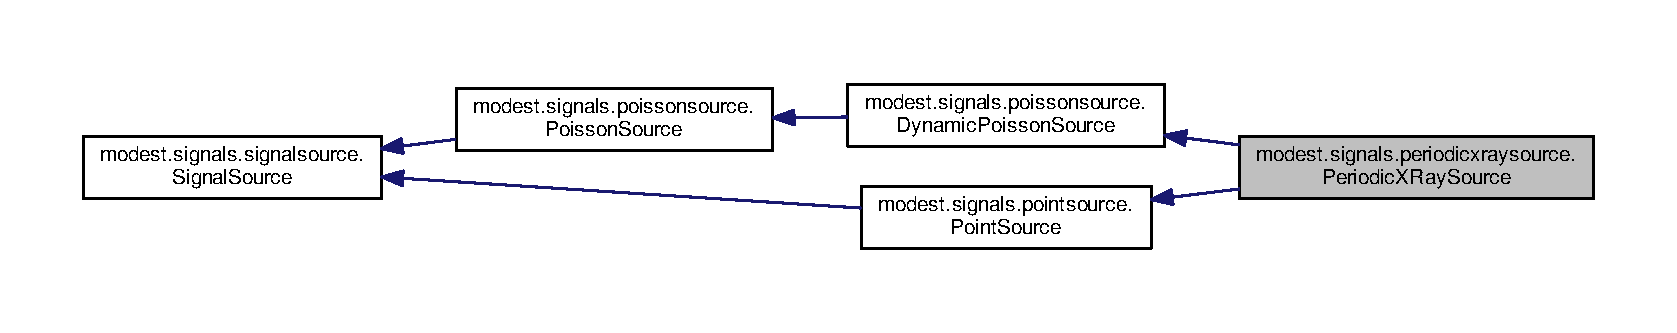
\includegraphics[width=350pt]{classmodest_1_1signals_1_1periodicxraysource_1_1PeriodicXRaySource__inherit__graph}
\end{center}
\end{figure}


Collaboration diagram for modest.\+signals.\+periodicxraysource.\+Periodic\+X\+Ray\+Source\+:
\nopagebreak
\begin{figure}[H]
\begin{center}
\leavevmode
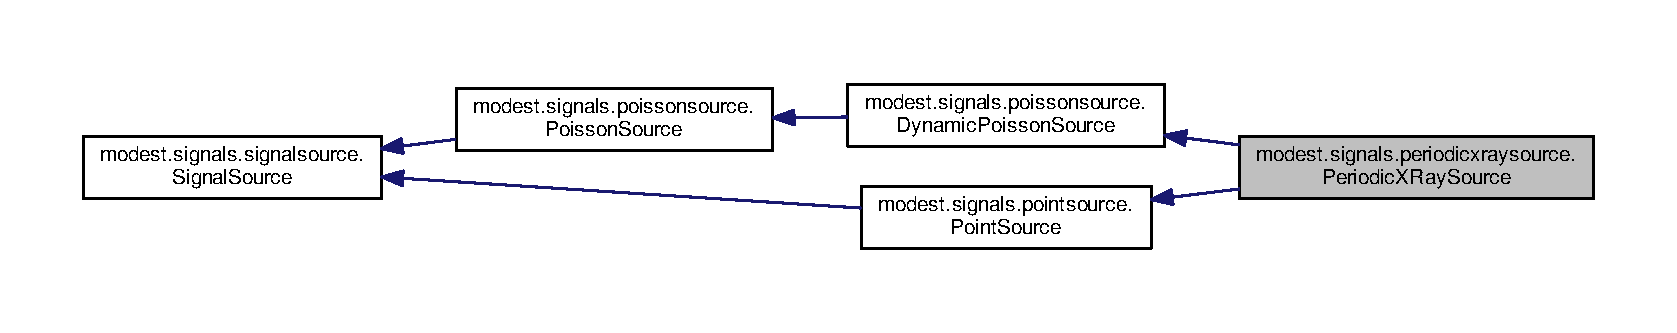
\includegraphics[width=350pt]{classmodest_1_1signals_1_1periodicxraysource_1_1PeriodicXRaySource__coll__graph}
\end{center}
\end{figure}
\subsection*{Public Member Functions}
\begin{DoxyCompactItemize}
\item 
def \hyperlink{classmodest_1_1signals_1_1periodicxraysource_1_1PeriodicXRaySource_a0aaaf0d5a5d2b15bb4c7ddefbaaab8c9}{\+\_\+\+\_\+init\+\_\+\+\_\+} (self, \hyperlink{classmodest_1_1signals_1_1periodicxraysource_1_1PeriodicXRaySource_a584d852c7e7be3d7a3ceb886575e9039}{profile}, \hyperlink{classmodest_1_1signals_1_1periodicxraysource_1_1PeriodicXRaySource_ab18463cedaf7e9ea17447e46f341bbb0}{avg\+Photon\+Flux}=None, \hyperlink{classmodest_1_1signals_1_1periodicxraysource_1_1PeriodicXRaySource_af76a5783d522dde15f37a9c48aa04391}{pulsed\+Fraction}=None, P\+A\+R\+File=None, move\+Peak\+To\+Zero=True, \hyperlink{classmodest_1_1signals_1_1periodicxraysource_1_1PeriodicXRaySource_a61df217b2685c2ccf9b0220044849a3c}{normalize\+Profile}=True, \hyperlink{classmodest_1_1signals_1_1periodicxraysource_1_1PeriodicXRaySource_aba99ee47fdedf6cb2fe5a78fc85d1baa}{phase\+Derivatives}=None, \hyperlink{classmodest_1_1signals_1_1periodicxraysource_1_1PeriodicXRaySource_a85fd954a8c19067087bbcb41a43a9f75}{pulsar\+Period}=None, RA=None, D\+EC=None, \hyperlink{classmodest_1_1signals_1_1periodicxraysource_1_1PeriodicXRaySource_a5300e5a9624bd81d7e2c8f2322653713}{observatory\+M\+J\+D\+R\+EF}=None, \hyperlink{classmodest_1_1signals_1_1periodicxraysource_1_1PeriodicXRaySource_a623878bc6ceaa59a60e0f3942768ba5c}{T\+Z\+R\+M\+JD}=None, \hyperlink{classmodest_1_1signals_1_1periodicxraysource_1_1PeriodicXRaySource_ae41de05104c0279bd59a47ff188020ea}{P\+E\+P\+O\+CH}=None, \hyperlink{classmodest_1_1signals_1_1periodicxraysource_1_1PeriodicXRaySource_aec42837776d331b803fe786647763be5}{name}=None, \hyperlink{classmodest_1_1signals_1_1pointsource_1_1PointSource_a0924a2233bb4fd23e50d024e4f1b048e}{attitude\+State\+Name}=\textquotesingle{}attitude\textquotesingle{}, \hyperlink{classmodest_1_1signals_1_1poissonsource_1_1DynamicPoissonSource_ac7f62303bb8a417a1ddefb032c707bcd}{correlation\+State\+Name}=None, use\+Profile\+Column=None, start\+Time=0, \hyperlink{classmodest_1_1signals_1_1pointsource_1_1PointSource_a984b5a75c9e94cb3527707b9ac976f9e}{extent}=0)
\item 
def \hyperlink{classmodest_1_1signals_1_1periodicxraysource_1_1PeriodicXRaySource_a9ee13a48b0501c8c8cbb662cd0d2c422}{process\+Profile} (self, \hyperlink{classmodest_1_1signals_1_1periodicxraysource_1_1PeriodicXRaySource_a584d852c7e7be3d7a3ceb886575e9039}{profile}, \hyperlink{classmodest_1_1signals_1_1periodicxraysource_1_1PeriodicXRaySource_a61df217b2685c2ccf9b0220044849a3c}{normalize\+Profile}=True, move\+Peak\+To\+Zero=True, use\+Profile\+Column=None)
\item 
def \hyperlink{classmodest_1_1signals_1_1periodicxraysource_1_1PeriodicXRaySource_a82addf4d6862423b3318da346cdb865e}{process\+P\+A\+R\+File} (self, P\+A\+R\+File, replace\+Current\+Values=False)
\item 
def \hyperlink{classmodest_1_1signals_1_1periodicxraysource_1_1PeriodicXRaySource_a3a07196809dc99abd81902fd7ed23eee}{compute\+Single\+Period\+Integral} (self)
\item 
def \hyperlink{classmodest_1_1signals_1_1periodicxraysource_1_1PeriodicXRaySource_aa1e5d06f2e4fd0908b7ba377162fa13f}{get\+Phase} (self, observatory\+Time)
\item 
def \hyperlink{classmodest_1_1signals_1_1periodicxraysource_1_1PeriodicXRaySource_a74531a4aacffcc59e47fda15793ede15}{get\+Frequency} (self, observatory\+Time)
\item 
def \hyperlink{classmodest_1_1signals_1_1periodicxraysource_1_1PeriodicXRaySource_a663b8e24a1d92b99a506a1b7e5535430}{get\+Period} (self, observatory\+Time)
\item 
def \hyperlink{classmodest_1_1signals_1_1periodicxraysource_1_1PeriodicXRaySource_a395746b94b58da20807c92633febffce}{get\+Signal\+M\+JD} (self, M\+JD)
\begin{DoxyCompactList}\small\item\em \hyperlink{classmodest_1_1signals_1_1periodicxraysource_1_1PeriodicXRaySource_a395746b94b58da20807c92633febffce}{get\+Signal\+M\+JD} is a wrapper function that returns the photon flux at a given Modified Julian Date \end{DoxyCompactList}\item 
def \hyperlink{classmodest_1_1signals_1_1periodicxraysource_1_1PeriodicXRaySource_a6cecf87c13cb6f104d9b7d45a3658fc8}{get\+Signal} (self, observatory\+Time, t\+Var=None)
\begin{DoxyCompactList}\small\item\em \hyperlink{classmodest_1_1signals_1_1periodicxraysource_1_1PeriodicXRaySource_a6cecf87c13cb6f104d9b7d45a3658fc8}{get\+Signal} is responsible for returning the photon flux from the pulsar at a given time \end{DoxyCompactList}\item 
def \hyperlink{classmodest_1_1signals_1_1periodicxraysource_1_1PeriodicXRaySource_ae933b6544c37c11a2298cb8fdd9d83a8}{signal\+Integral} (self, t\+Start, t\+Stop, state=None)
\item 
def \hyperlink{classmodest_1_1signals_1_1periodicxraysource_1_1PeriodicXRaySource_a0f4b278270d67daf1ecd3c1829de575f}{get\+Pulse\+From\+Phase} (self, phase)
\item 
def \hyperlink{classmodest_1_1signals_1_1periodicxraysource_1_1PeriodicXRaySource_a75b3899dab7d513677ec0057078a6e11}{M\+J\+D2seconds} (self, M\+JD)
\item 
def \hyperlink{classmodest_1_1signals_1_1periodicxraysource_1_1PeriodicXRaySource_a05579d0ee00b0070689a5472e2d078df}{seconds2\+M\+JD} (self, seconds)
\item 
def \hyperlink{classmodest_1_1signals_1_1periodicxraysource_1_1PeriodicXRaySource_aa978de937dca63b09fdc00a8ab927966}{compute\+Association\+Probability} (self, measurement, state\+Dict, validation\+Threshold=0)
\item 
def \hyperlink{classmodest_1_1signals_1_1periodicxraysource_1_1PeriodicXRaySource_aac2cb4da7cca8856c598e1e5a744796c}{plot} (self, n\+Periods=1, t\+Var=None, figure\+Handle=None, n\+Points=1000)
\item 
def \hyperlink{classmodest_1_1signals_1_1periodicxraysource_1_1PeriodicXRaySource_aa2cac6c15e836a557255a4b8e9ffb289}{generate\+Photon\+Arrivals} (self, t\+Max, t0=0, position=None, attitude=None, F\+OV=None, A\+O\+A\+\_\+\+Std\+Dev=None, T\+O\+A\+\_\+\+Std\+Dev=None)
\item 
def \hyperlink{classmodest_1_1signals_1_1periodicxraysource_1_1PeriodicXRaySource_ab14c776a1c0b691a509eb423da85227c}{speed\+Of\+Light} (self)
\item 
def \hyperlink{classmodest_1_1signals_1_1poissonsource_1_1DynamicPoissonSource_a01804453d22cab5811218a98557a8b0c}{get\+Signal} (self, t, t\+Var=None, state=None)
\item 
def \hyperlink{classmodest_1_1signals_1_1poissonsource_1_1DynamicPoissonSource_a6c8820d8007c848d745f9313efdb970c}{compute\+Association\+Probability} (self, measurement, state\+Dict)
\item 
def \hyperlink{classmodest_1_1signals_1_1signalsource_1_1SignalSource_a9a64c6a9c2954f6ad61e4ca3518ea8ab}{signal\+ID} (self)
\item 
def \hyperlink{classmodest_1_1signals_1_1pointsource_1_1PointSource_a295eb1a487e18c77029585ac2785db80}{Ra\+Dec} (self)
\item 
def \hyperlink{classmodest_1_1signals_1_1pointsource_1_1PointSource_a133933430a784107258901e257778221}{unit\+Vec} (self, \hyperlink{classmodest_1_1signals_1_1pointsource_1_1PointSource_a295eb1a487e18c77029585ac2785db80}{Ra\+Dec}=None)
\item 
def \hyperlink{classmodest_1_1signals_1_1pointsource_1_1PointSource_abf359a17cf5bec4c51deef87c9e92cce}{generate\+Arrival\+Vector} (self, attitudeQ, A\+O\+A\+\_\+\+Std\+Dev=None)
\item 
def \hyperlink{classmodest_1_1signals_1_1signalsource_1_1SignalSource_a9a64c6a9c2954f6ad61e4ca3518ea8ab}{signal\+ID} (self)
\end{DoxyCompactItemize}
\subsection*{Public Attributes}
\begin{DoxyCompactItemize}
\item 
\hyperlink{classmodest_1_1signals_1_1periodicxraysource_1_1PeriodicXRaySource_aba99ee47fdedf6cb2fe5a78fc85d1baa}{phase\+Derivatives}
\begin{DoxyCompactList}\small\item\em Stores the derivatives of phase with respect to time  \hyperlink{classmodest_1_1signals_1_1periodicxraysource_1_1PeriodicXRaySource_aba99ee47fdedf6cb2fe5a78fc85d1baa}{phase\+Derivatives} is a dict which contains the derivatives of phase with respect to time. \end{DoxyCompactList}\item 
\hyperlink{classmodest_1_1signals_1_1periodicxraysource_1_1PeriodicXRaySource_a623878bc6ceaa59a60e0f3942768ba5c}{T\+Z\+R\+M\+JD}
\begin{DoxyCompactList}\small\item\em \hyperlink{classmodest_1_1signals_1_1periodicxraysource_1_1PeriodicXRaySource_a623878bc6ceaa59a60e0f3942768ba5c}{T\+Z\+R\+M\+JD} stores the Modified Julian Date (M\+JD) corresponding to t=0 seconds (for the purpose of computing the pulsar phase) \end{DoxyCompactList}\item 
\hyperlink{classmodest_1_1signals_1_1periodicxraysource_1_1PeriodicXRaySource_ae41de05104c0279bd59a47ff188020ea}{P\+E\+P\+O\+CH}
\item 
\hyperlink{classmodest_1_1signals_1_1periodicxraysource_1_1PeriodicXRaySource_a5300e5a9624bd81d7e2c8f2322653713}{observatory\+M\+J\+D\+R\+EF}
\begin{DoxyCompactList}\small\item\em \hyperlink{classmodest_1_1signals_1_1periodicxraysource_1_1PeriodicXRaySource_a5300e5a9624bd81d7e2c8f2322653713}{observatory\+M\+J\+D\+R\+EF} stores the M\+JD corresponding to t=0 seconds for photon observations \end{DoxyCompactList}\item 
\hyperlink{classmodest_1_1signals_1_1periodicxraysource_1_1PeriodicXRaySource_aec42837776d331b803fe786647763be5}{name}
\begin{DoxyCompactList}\small\item\em \hyperlink{classmodest_1_1signals_1_1periodicxraysource_1_1PeriodicXRaySource_aec42837776d331b803fe786647763be5}{name} is an arbitrary string that is used to identify the signal. \end{DoxyCompactList}\item 
\hyperlink{classmodest_1_1signals_1_1periodicxraysource_1_1PeriodicXRaySource_ab18463cedaf7e9ea17447e46f341bbb0}{avg\+Photon\+Flux}
\begin{DoxyCompactList}\small\item\em \#average\+Photon\+Flux is the mean value of photons expected to arrive from the signal per second (units of photons/second) \end{DoxyCompactList}\item 
\hyperlink{classmodest_1_1signals_1_1periodicxraysource_1_1PeriodicXRaySource_af76a5783d522dde15f37a9c48aa04391}{pulsed\+Fraction}
\begin{DoxyCompactList}\small\item\em \hyperlink{classmodest_1_1signals_1_1periodicxraysource_1_1PeriodicXRaySource_af76a5783d522dde15f37a9c48aa04391}{pulsed\+Fraction} is a value from 0 to 1 which indicates what percentage of the \hyperlink{classmodest_1_1signals_1_1periodicxraysource_1_1PeriodicXRaySource_ab18463cedaf7e9ea17447e46f341bbb0}{avg\+Photon\+Flux} is \char`\"{}pulsed\char`\"{} and what percentage is constant/background \end{DoxyCompactList}\item 
\hyperlink{classmodest_1_1signals_1_1periodicxraysource_1_1PeriodicXRaySource_a61df217b2685c2ccf9b0220044849a3c}{normalize\+Profile}
\begin{DoxyCompactList}\small\item\em \hyperlink{classmodest_1_1signals_1_1periodicxraysource_1_1PeriodicXRaySource_a61df217b2685c2ccf9b0220044849a3c}{normalize\+Profile} is a boolean flag used to indicate whether the profile is normalized from zero to one. \end{DoxyCompactList}\item 
\hyperlink{classmodest_1_1signals_1_1periodicxraysource_1_1PeriodicXRaySource_ac8781ace6f2f18d79a5114a0ce6224cc}{T\+Zero\+Diff}
\item 
\hyperlink{classmodest_1_1signals_1_1periodicxraysource_1_1PeriodicXRaySource_a85fd954a8c19067087bbcb41a43a9f75}{pulsar\+Period}
\begin{DoxyCompactList}\small\item\em \hyperlink{classmodest_1_1signals_1_1periodicxraysource_1_1PeriodicXRaySource_a85fd954a8c19067087bbcb41a43a9f75}{pulsar\+Period} is the amouont of time (in seconds) for one complete pulsar pulse. \end{DoxyCompactList}\item 
\hyperlink{classmodest_1_1signals_1_1periodicxraysource_1_1PeriodicXRaySource_a584d852c7e7be3d7a3ceb886575e9039}{profile}
\begin{DoxyCompactList}\small\item\em \hyperlink{classmodest_1_1signals_1_1periodicxraysource_1_1PeriodicXRaySource_a584d852c7e7be3d7a3ceb886575e9039}{profile} is a numpy array containing the numerical value of flux over a single period of the signal. \end{DoxyCompactList}\item 
\hyperlink{classmodest_1_1signals_1_1periodicxraysource_1_1PeriodicXRaySource_a008ccf30a31f3d1641df7c2504b95523}{profile\+Index}
\item 
\hyperlink{classmodest_1_1signals_1_1periodicxraysource_1_1PeriodicXRaySource_a387d8eb4fb739b49b8a51fe687a45082}{single\+Period\+Integral}
\item 
\hyperlink{classmodest_1_1signals_1_1periodicxraysource_1_1PeriodicXRaySource_ac1eeb6c4af724737f6568e2ad8f1e05c}{profile\+Len}
\item 
\hyperlink{classmodest_1_1signals_1_1periodicxraysource_1_1PeriodicXRaySource_ad8a98679b8f8b313457be3519bbc6fe2}{photons\+Per\+Period}
\item 
\hyperlink{classmodest_1_1signals_1_1periodicxraysource_1_1PeriodicXRaySource_a50a65021397b8cab83f2941e9b2d9036}{peak\+Amplitude}
\item 
\hyperlink{classmodest_1_1signals_1_1periodicxraysource_1_1PeriodicXRaySource_aa54bef8e6c3c0b7d9d8321897dd4eb27}{scale\+Factor}
\item 
\hyperlink{classmodest_1_1signals_1_1periodicxraysource_1_1PeriodicXRaySource_a27d4737b3a521750007ab14954802876}{background\+Count\+Rate}
\item 
\hyperlink{classmodest_1_1signals_1_1poissonsource_1_1DynamicPoissonSource_ac7f62303bb8a417a1ddefb032c707bcd}{correlation\+State\+Name}
\item 
\hyperlink{classmodest_1_1signals_1_1poissonsource_1_1PoissonSource_a34395fc83bd8743a0a5ee69f9392a606}{last\+Time}
\item 
\hyperlink{classmodest_1_1signals_1_1poissonsource_1_1PoissonSource_a6f2c657ad936b921715d826ac74f7fe5}{flux}
\item 
\hyperlink{classmodest_1_1signals_1_1pointsource_1_1PointSource_ac2dd52c4e1f7e6264c9d59a5ffbc43d1}{use\+Unit\+Vector}
\item 
\hyperlink{classmodest_1_1signals_1_1pointsource_1_1PointSource_a0924a2233bb4fd23e50d024e4f1b048e}{attitude\+State\+Name}
\item 
\hyperlink{classmodest_1_1signals_1_1pointsource_1_1PointSource_afde4a069238f53aaa11fbc54584b7a64}{last\+P\+DF}
\item 
\hyperlink{classmodest_1_1signals_1_1pointsource_1_1PointSource_a984b5a75c9e94cb3527707b9ac976f9e}{extent}
\end{DoxyCompactItemize}
\subsection*{Static Public Attributes}
\begin{DoxyCompactItemize}
\item 
int \hyperlink{classmodest_1_1signals_1_1signalsource_1_1SignalSource_a453eafb550b551adbec0903deb63dfce}{next\+Signal\+ID} = 0
\item 
int \hyperlink{classmodest_1_1signals_1_1signalsource_1_1SignalSource_a453eafb550b551adbec0903deb63dfce}{next\+Signal\+ID} = 0
\end{DoxyCompactItemize}


\subsection{Detailed Description}


Definition at line 18 of file periodicxraysource.\+py.



\subsection{Constructor \& Destructor Documentation}
\index{modest\+::signals\+::periodicxraysource\+::\+Periodic\+X\+Ray\+Source@{modest\+::signals\+::periodicxraysource\+::\+Periodic\+X\+Ray\+Source}!\+\_\+\+\_\+init\+\_\+\+\_\+@{\+\_\+\+\_\+init\+\_\+\+\_\+}}
\index{\+\_\+\+\_\+init\+\_\+\+\_\+@{\+\_\+\+\_\+init\+\_\+\+\_\+}!modest\+::signals\+::periodicxraysource\+::\+Periodic\+X\+Ray\+Source@{modest\+::signals\+::periodicxraysource\+::\+Periodic\+X\+Ray\+Source}}
\subsubsection[{\texorpdfstring{\+\_\+\+\_\+init\+\_\+\+\_\+(self, profile, avg\+Photon\+Flux=\+None, pulsed\+Fraction=\+None, P\+A\+R\+File=\+None, move\+Peak\+To\+Zero=\+True, normalize\+Profile=\+True, phase\+Derivatives=\+None, pulsar\+Period=\+None, R\+A=\+None, D\+E\+C=\+None, observatory\+M\+J\+D\+R\+E\+F=\+None, T\+Z\+R\+M\+J\+D=\+None, P\+E\+P\+O\+C\+H=\+None, name=\+None, attitude\+State\+Name=\textquotesingle{}attitude\textquotesingle{}, correlation\+State\+Name=\+None, use\+Profile\+Column=\+None, start\+Time=0, extent=0)}{__init__(self, profile, avgPhotonFlux=None, pulsedFraction=None, PARFile=None, movePeakToZero=True, normalizeProfile=True, phaseDerivatives=None, pulsarPeriod=None, RA=None, DEC=None, observatoryMJDREF=None, TZRMJD=None, PEPOCH=None, name=None, attitudeStateName='attitude', correlationStateName=None, useProfileColumn=None, startTime=0, extent=0)}}]{\setlength{\rightskip}{0pt plus 5cm}def modest.\+signals.\+periodicxraysource.\+Periodic\+X\+Ray\+Source.\+\_\+\+\_\+init\+\_\+\+\_\+ (
\begin{DoxyParamCaption}
\item[{}]{self, }
\item[{}]{profile, }
\item[{}]{avg\+Photon\+Flux = {\ttfamily None}, }
\item[{}]{pulsed\+Fraction = {\ttfamily None}, }
\item[{}]{P\+A\+R\+File = {\ttfamily None}, }
\item[{}]{move\+Peak\+To\+Zero = {\ttfamily True}, }
\item[{}]{normalize\+Profile = {\ttfamily True}, }
\item[{}]{phase\+Derivatives = {\ttfamily None}, }
\item[{}]{pulsar\+Period = {\ttfamily None}, }
\item[{}]{RA = {\ttfamily None}, }
\item[{}]{D\+EC = {\ttfamily None}, }
\item[{}]{observatory\+M\+J\+D\+R\+EF = {\ttfamily None}, }
\item[{}]{T\+Z\+R\+M\+JD = {\ttfamily None}, }
\item[{}]{P\+E\+P\+O\+CH = {\ttfamily None}, }
\item[{}]{name = {\ttfamily None}, }
\item[{}]{attitude\+State\+Name = {\ttfamily \textquotesingle{}attitude\textquotesingle{}}, }
\item[{}]{correlation\+State\+Name = {\ttfamily None}, }
\item[{}]{use\+Profile\+Column = {\ttfamily None}, }
\item[{}]{start\+Time = {\ttfamily 0}, }
\item[{}]{extent = {\ttfamily 0}}
\end{DoxyParamCaption}
)}\hypertarget{classmodest_1_1signals_1_1periodicxraysource_1_1PeriodicXRaySource_a0aaaf0d5a5d2b15bb4c7ddefbaaab8c9}{}\label{classmodest_1_1signals_1_1periodicxraysource_1_1PeriodicXRaySource_a0aaaf0d5a5d2b15bb4c7ddefbaaab8c9}


Definition at line 40 of file periodicxraysource.\+py.



\subsection{Member Function Documentation}
\index{modest\+::signals\+::periodicxraysource\+::\+Periodic\+X\+Ray\+Source@{modest\+::signals\+::periodicxraysource\+::\+Periodic\+X\+Ray\+Source}!compute\+Association\+Probability@{compute\+Association\+Probability}}
\index{compute\+Association\+Probability@{compute\+Association\+Probability}!modest\+::signals\+::periodicxraysource\+::\+Periodic\+X\+Ray\+Source@{modest\+::signals\+::periodicxraysource\+::\+Periodic\+X\+Ray\+Source}}
\subsubsection[{\texorpdfstring{compute\+Association\+Probability(self, measurement, state\+Dict)}{computeAssociationProbability(self, measurement, stateDict)}}]{\setlength{\rightskip}{0pt plus 5cm}def modest.\+signals.\+poissonsource.\+Dynamic\+Poisson\+Source.\+compute\+Association\+Probability (
\begin{DoxyParamCaption}
\item[{}]{self, }
\item[{}]{measurement, }
\item[{}]{state\+Dict}
\end{DoxyParamCaption}
)\hspace{0.3cm}{\ttfamily [inherited]}}\hypertarget{classmodest_1_1signals_1_1poissonsource_1_1DynamicPoissonSource_a6c8820d8007c848d745f9313efdb970c}{}\label{classmodest_1_1signals_1_1poissonsource_1_1DynamicPoissonSource_a6c8820d8007c848d745f9313efdb970c}


Definition at line 113 of file poissonsource.\+py.

\index{modest\+::signals\+::periodicxraysource\+::\+Periodic\+X\+Ray\+Source@{modest\+::signals\+::periodicxraysource\+::\+Periodic\+X\+Ray\+Source}!compute\+Association\+Probability@{compute\+Association\+Probability}}
\index{compute\+Association\+Probability@{compute\+Association\+Probability}!modest\+::signals\+::periodicxraysource\+::\+Periodic\+X\+Ray\+Source@{modest\+::signals\+::periodicxraysource\+::\+Periodic\+X\+Ray\+Source}}
\subsubsection[{\texorpdfstring{compute\+Association\+Probability(self, measurement, state\+Dict, validation\+Threshold=0)}{computeAssociationProbability(self, measurement, stateDict, validationThreshold=0)}}]{\setlength{\rightskip}{0pt plus 5cm}def modest.\+signals.\+periodicxraysource.\+Periodic\+X\+Ray\+Source.\+compute\+Association\+Probability (
\begin{DoxyParamCaption}
\item[{}]{self, }
\item[{}]{measurement, }
\item[{}]{state\+Dict, }
\item[{}]{validation\+Threshold = {\ttfamily 0}}
\end{DoxyParamCaption}
)}\hypertarget{classmodest_1_1signals_1_1periodicxraysource_1_1PeriodicXRaySource_aa978de937dca63b09fdc00a8ab927966}{}\label{classmodest_1_1signals_1_1periodicxraysource_1_1PeriodicXRaySource_aa978de937dca63b09fdc00a8ab927966}


Definition at line 586 of file periodicxraysource.\+py.

\index{modest\+::signals\+::periodicxraysource\+::\+Periodic\+X\+Ray\+Source@{modest\+::signals\+::periodicxraysource\+::\+Periodic\+X\+Ray\+Source}!compute\+Single\+Period\+Integral@{compute\+Single\+Period\+Integral}}
\index{compute\+Single\+Period\+Integral@{compute\+Single\+Period\+Integral}!modest\+::signals\+::periodicxraysource\+::\+Periodic\+X\+Ray\+Source@{modest\+::signals\+::periodicxraysource\+::\+Periodic\+X\+Ray\+Source}}
\subsubsection[{\texorpdfstring{compute\+Single\+Period\+Integral(self)}{computeSinglePeriodIntegral(self)}}]{\setlength{\rightskip}{0pt plus 5cm}def modest.\+signals.\+periodicxraysource.\+Periodic\+X\+Ray\+Source.\+compute\+Single\+Period\+Integral (
\begin{DoxyParamCaption}
\item[{}]{self}
\end{DoxyParamCaption}
)}\hypertarget{classmodest_1_1signals_1_1periodicxraysource_1_1PeriodicXRaySource_a3a07196809dc99abd81902fd7ed23eee}{}\label{classmodest_1_1signals_1_1periodicxraysource_1_1PeriodicXRaySource_a3a07196809dc99abd81902fd7ed23eee}


Definition at line 291 of file periodicxraysource.\+py.

\index{modest\+::signals\+::periodicxraysource\+::\+Periodic\+X\+Ray\+Source@{modest\+::signals\+::periodicxraysource\+::\+Periodic\+X\+Ray\+Source}!generate\+Arrival\+Vector@{generate\+Arrival\+Vector}}
\index{generate\+Arrival\+Vector@{generate\+Arrival\+Vector}!modest\+::signals\+::periodicxraysource\+::\+Periodic\+X\+Ray\+Source@{modest\+::signals\+::periodicxraysource\+::\+Periodic\+X\+Ray\+Source}}
\subsubsection[{\texorpdfstring{generate\+Arrival\+Vector(self, attitude\+Q, A\+O\+A\+\_\+\+Std\+Dev=\+None)}{generateArrivalVector(self, attitudeQ, AOA_StdDev=None)}}]{\setlength{\rightskip}{0pt plus 5cm}def modest.\+signals.\+pointsource.\+Point\+Source.\+generate\+Arrival\+Vector (
\begin{DoxyParamCaption}
\item[{}]{self, }
\item[{}]{attitudeQ, }
\item[{}]{A\+O\+A\+\_\+\+Std\+Dev = {\ttfamily None}}
\end{DoxyParamCaption}
)\hspace{0.3cm}{\ttfamily [inherited]}}\hypertarget{classmodest_1_1signals_1_1pointsource_1_1PointSource_abf359a17cf5bec4c51deef87c9e92cce}{}\label{classmodest_1_1signals_1_1pointsource_1_1PointSource_abf359a17cf5bec4c51deef87c9e92cce}


Definition at line 143 of file pointsource.\+py.

\index{modest\+::signals\+::periodicxraysource\+::\+Periodic\+X\+Ray\+Source@{modest\+::signals\+::periodicxraysource\+::\+Periodic\+X\+Ray\+Source}!generate\+Photon\+Arrivals@{generate\+Photon\+Arrivals}}
\index{generate\+Photon\+Arrivals@{generate\+Photon\+Arrivals}!modest\+::signals\+::periodicxraysource\+::\+Periodic\+X\+Ray\+Source@{modest\+::signals\+::periodicxraysource\+::\+Periodic\+X\+Ray\+Source}}
\subsubsection[{\texorpdfstring{generate\+Photon\+Arrivals(self, t\+Max, t0=0, position=\+None, attitude=\+None, F\+O\+V=\+None, A\+O\+A\+\_\+\+Std\+Dev=\+None, T\+O\+A\+\_\+\+Std\+Dev=\+None)}{generatePhotonArrivals(self, tMax, t0=0, position=None, attitude=None, FOV=None, AOA_StdDev=None, TOA_StdDev=None)}}]{\setlength{\rightskip}{0pt plus 5cm}def modest.\+signals.\+periodicxraysource.\+Periodic\+X\+Ray\+Source.\+generate\+Photon\+Arrivals (
\begin{DoxyParamCaption}
\item[{}]{self, }
\item[{}]{t\+Max, }
\item[{}]{t0 = {\ttfamily 0}, }
\item[{}]{position = {\ttfamily None}, }
\item[{}]{attitude = {\ttfamily None}, }
\item[{}]{F\+OV = {\ttfamily None}, }
\item[{}]{A\+O\+A\+\_\+\+Std\+Dev = {\ttfamily None}, }
\item[{}]{T\+O\+A\+\_\+\+Std\+Dev = {\ttfamily None}}
\end{DoxyParamCaption}
)}\hypertarget{classmodest_1_1signals_1_1periodicxraysource_1_1PeriodicXRaySource_aa2cac6c15e836a557255a4b8e9ffb289}{}\label{classmodest_1_1signals_1_1periodicxraysource_1_1PeriodicXRaySource_aa2cac6c15e836a557255a4b8e9ffb289}


Definition at line 645 of file periodicxraysource.\+py.

\index{modest\+::signals\+::periodicxraysource\+::\+Periodic\+X\+Ray\+Source@{modest\+::signals\+::periodicxraysource\+::\+Periodic\+X\+Ray\+Source}!get\+Frequency@{get\+Frequency}}
\index{get\+Frequency@{get\+Frequency}!modest\+::signals\+::periodicxraysource\+::\+Periodic\+X\+Ray\+Source@{modest\+::signals\+::periodicxraysource\+::\+Periodic\+X\+Ray\+Source}}
\subsubsection[{\texorpdfstring{get\+Frequency(self, observatory\+Time)}{getFrequency(self, observatoryTime)}}]{\setlength{\rightskip}{0pt plus 5cm}def modest.\+signals.\+periodicxraysource.\+Periodic\+X\+Ray\+Source.\+get\+Frequency (
\begin{DoxyParamCaption}
\item[{}]{self, }
\item[{}]{observatory\+Time}
\end{DoxyParamCaption}
)}\hypertarget{classmodest_1_1signals_1_1periodicxraysource_1_1PeriodicXRaySource_a74531a4aacffcc59e47fda15793ede15}{}\label{classmodest_1_1signals_1_1periodicxraysource_1_1PeriodicXRaySource_a74531a4aacffcc59e47fda15793ede15}


Definition at line 367 of file periodicxraysource.\+py.

\index{modest\+::signals\+::periodicxraysource\+::\+Periodic\+X\+Ray\+Source@{modest\+::signals\+::periodicxraysource\+::\+Periodic\+X\+Ray\+Source}!get\+Period@{get\+Period}}
\index{get\+Period@{get\+Period}!modest\+::signals\+::periodicxraysource\+::\+Periodic\+X\+Ray\+Source@{modest\+::signals\+::periodicxraysource\+::\+Periodic\+X\+Ray\+Source}}
\subsubsection[{\texorpdfstring{get\+Period(self, observatory\+Time)}{getPeriod(self, observatoryTime)}}]{\setlength{\rightskip}{0pt plus 5cm}def modest.\+signals.\+periodicxraysource.\+Periodic\+X\+Ray\+Source.\+get\+Period (
\begin{DoxyParamCaption}
\item[{}]{self, }
\item[{}]{observatory\+Time}
\end{DoxyParamCaption}
)}\hypertarget{classmodest_1_1signals_1_1periodicxraysource_1_1PeriodicXRaySource_a663b8e24a1d92b99a506a1b7e5535430}{}\label{classmodest_1_1signals_1_1periodicxraysource_1_1PeriodicXRaySource_a663b8e24a1d92b99a506a1b7e5535430}


Definition at line 385 of file periodicxraysource.\+py.

\index{modest\+::signals\+::periodicxraysource\+::\+Periodic\+X\+Ray\+Source@{modest\+::signals\+::periodicxraysource\+::\+Periodic\+X\+Ray\+Source}!get\+Phase@{get\+Phase}}
\index{get\+Phase@{get\+Phase}!modest\+::signals\+::periodicxraysource\+::\+Periodic\+X\+Ray\+Source@{modest\+::signals\+::periodicxraysource\+::\+Periodic\+X\+Ray\+Source}}
\subsubsection[{\texorpdfstring{get\+Phase(self, observatory\+Time)}{getPhase(self, observatoryTime)}}]{\setlength{\rightskip}{0pt plus 5cm}def modest.\+signals.\+periodicxraysource.\+Periodic\+X\+Ray\+Source.\+get\+Phase (
\begin{DoxyParamCaption}
\item[{}]{self, }
\item[{}]{observatory\+Time}
\end{DoxyParamCaption}
)}\hypertarget{classmodest_1_1signals_1_1periodicxraysource_1_1PeriodicXRaySource_aa1e5d06f2e4fd0908b7ba377162fa13f}{}\label{classmodest_1_1signals_1_1periodicxraysource_1_1PeriodicXRaySource_aa1e5d06f2e4fd0908b7ba377162fa13f}


Definition at line 350 of file periodicxraysource.\+py.

\index{modest\+::signals\+::periodicxraysource\+::\+Periodic\+X\+Ray\+Source@{modest\+::signals\+::periodicxraysource\+::\+Periodic\+X\+Ray\+Source}!get\+Pulse\+From\+Phase@{get\+Pulse\+From\+Phase}}
\index{get\+Pulse\+From\+Phase@{get\+Pulse\+From\+Phase}!modest\+::signals\+::periodicxraysource\+::\+Periodic\+X\+Ray\+Source@{modest\+::signals\+::periodicxraysource\+::\+Periodic\+X\+Ray\+Source}}
\subsubsection[{\texorpdfstring{get\+Pulse\+From\+Phase(self, phase)}{getPulseFromPhase(self, phase)}}]{\setlength{\rightskip}{0pt plus 5cm}def modest.\+signals.\+periodicxraysource.\+Periodic\+X\+Ray\+Source.\+get\+Pulse\+From\+Phase (
\begin{DoxyParamCaption}
\item[{}]{self, }
\item[{}]{phase}
\end{DoxyParamCaption}
)}\hypertarget{classmodest_1_1signals_1_1periodicxraysource_1_1PeriodicXRaySource_a0f4b278270d67daf1ecd3c1829de575f}{}\label{classmodest_1_1signals_1_1periodicxraysource_1_1PeriodicXRaySource_a0f4b278270d67daf1ecd3c1829de575f}


Definition at line 563 of file periodicxraysource.\+py.

\index{modest\+::signals\+::periodicxraysource\+::\+Periodic\+X\+Ray\+Source@{modest\+::signals\+::periodicxraysource\+::\+Periodic\+X\+Ray\+Source}!get\+Signal@{get\+Signal}}
\index{get\+Signal@{get\+Signal}!modest\+::signals\+::periodicxraysource\+::\+Periodic\+X\+Ray\+Source@{modest\+::signals\+::periodicxraysource\+::\+Periodic\+X\+Ray\+Source}}
\subsubsection[{\texorpdfstring{get\+Signal(self, t, t\+Var=\+None, state=\+None)}{getSignal(self, t, tVar=None, state=None)}}]{\setlength{\rightskip}{0pt plus 5cm}def modest.\+signals.\+poissonsource.\+Dynamic\+Poisson\+Source.\+get\+Signal (
\begin{DoxyParamCaption}
\item[{}]{self, }
\item[{}]{t, }
\item[{}]{t\+Var = {\ttfamily None}, }
\item[{}]{state = {\ttfamily None}}
\end{DoxyParamCaption}
)\hspace{0.3cm}{\ttfamily [inherited]}}\hypertarget{classmodest_1_1signals_1_1poissonsource_1_1DynamicPoissonSource_a01804453d22cab5811218a98557a8b0c}{}\label{classmodest_1_1signals_1_1poissonsource_1_1DynamicPoissonSource_a01804453d22cab5811218a98557a8b0c}


Definition at line 103 of file poissonsource.\+py.

\index{modest\+::signals\+::periodicxraysource\+::\+Periodic\+X\+Ray\+Source@{modest\+::signals\+::periodicxraysource\+::\+Periodic\+X\+Ray\+Source}!get\+Signal@{get\+Signal}}
\index{get\+Signal@{get\+Signal}!modest\+::signals\+::periodicxraysource\+::\+Periodic\+X\+Ray\+Source@{modest\+::signals\+::periodicxraysource\+::\+Periodic\+X\+Ray\+Source}}
\subsubsection[{\texorpdfstring{get\+Signal(self, observatory\+Time, t\+Var=\+None)}{getSignal(self, observatoryTime, tVar=None)}}]{\setlength{\rightskip}{0pt plus 5cm}def modest.\+signals.\+periodicxraysource.\+Periodic\+X\+Ray\+Source.\+get\+Signal (
\begin{DoxyParamCaption}
\item[{}]{self, }
\item[{}]{observatory\+Time, }
\item[{}]{t\+Var = {\ttfamily None}}
\end{DoxyParamCaption}
)}\hypertarget{classmodest_1_1signals_1_1periodicxraysource_1_1PeriodicXRaySource_a6cecf87c13cb6f104d9b7d45a3658fc8}{}\label{classmodest_1_1signals_1_1periodicxraysource_1_1PeriodicXRaySource_a6cecf87c13cb6f104d9b7d45a3658fc8}


\hyperlink{classmodest_1_1signals_1_1periodicxraysource_1_1PeriodicXRaySource_a6cecf87c13cb6f104d9b7d45a3658fc8}{get\+Signal} is responsible for returning the photon flux from the pulsar at a given time 

The \hyperlink{classmodest_1_1signals_1_1periodicxraysource_1_1PeriodicXRaySource_a6cecf87c13cb6f104d9b7d45a3658fc8}{get\+Signal} method is the method which is responsible for returning the current value of flux from the signal source at a given time. If there is uncertainty in the time, then the expected value of the signal is returned. Uncertainty in time is indicated by the optional t\+Var argument.

In every case, the method calls the \hyperlink{classmodest_1_1signals_1_1periodicxraysource_1_1PeriodicXRaySource_aa1e5d06f2e4fd0908b7ba377162fa13f}{get\+Phase} method to determine the current signal source phase. If no uncertainty in time is passed, then the \hyperlink{classmodest_1_1signals_1_1periodicxraysource_1_1PeriodicXRaySource_a0f4b278270d67daf1ecd3c1829de575f}{get\+Pulse\+From\+Phase} method is called to lookup/interpolate the current flux based on the phase and the signal \hyperlink{classmodest_1_1signals_1_1periodicxraysource_1_1PeriodicXRaySource_a584d852c7e7be3d7a3ceb886575e9039}{profile}.

If a value is passed for t\+Var, then the process is more complicated. Rather than simply look up the signal value from the phase, the function returns an approximation of the expected value of the signal, given the mean and variance of time.

Normally, the expected value would be computed by integrating the product of the true distribution of time (probably a normal distribution) with the flux as a function of time. However, due to the non-\/analytical nature of the flux function, the direct computation of this integral is intractable. To overcome this limitation, the time distributuion is approximated as a moment-\/matched uniform distribution. Using this approximation, the approximate integral may be directly computed simply by looking up the start and end values of \hyperlink{classmodest_1_1signals_1_1periodicxraysource_1_1PeriodicXRaySource_a387d8eb4fb739b49b8a51fe687a45082}{single\+Period\+Integral}, and dividing by the appropriate scaling factor.


\begin{DoxyParams}{Parameters}
{\em self} & The object pointer \\
\hline
{\em observatory\+Time} & The time for which to compute the signal \\
\hline
{\em t\+Var} & (optional) The variance of the time estimate\\
\hline
\end{DoxyParams}
\begin{DoxyReturn}{Returns}
The signal at the requested time 
\end{DoxyReturn}


Definition at line 442 of file periodicxraysource.\+py.

\index{modest\+::signals\+::periodicxraysource\+::\+Periodic\+X\+Ray\+Source@{modest\+::signals\+::periodicxraysource\+::\+Periodic\+X\+Ray\+Source}!get\+Signal\+M\+JD@{get\+Signal\+M\+JD}}
\index{get\+Signal\+M\+JD@{get\+Signal\+M\+JD}!modest\+::signals\+::periodicxraysource\+::\+Periodic\+X\+Ray\+Source@{modest\+::signals\+::periodicxraysource\+::\+Periodic\+X\+Ray\+Source}}
\subsubsection[{\texorpdfstring{get\+Signal\+M\+J\+D(self, M\+J\+D)}{getSignalMJD(self, MJD)}}]{\setlength{\rightskip}{0pt plus 5cm}def modest.\+signals.\+periodicxraysource.\+Periodic\+X\+Ray\+Source.\+get\+Signal\+M\+JD (
\begin{DoxyParamCaption}
\item[{}]{self, }
\item[{}]{M\+JD}
\end{DoxyParamCaption}
)}\hypertarget{classmodest_1_1signals_1_1periodicxraysource_1_1PeriodicXRaySource_a395746b94b58da20807c92633febffce}{}\label{classmodest_1_1signals_1_1periodicxraysource_1_1PeriodicXRaySource_a395746b94b58da20807c92633febffce}


\hyperlink{classmodest_1_1signals_1_1periodicxraysource_1_1PeriodicXRaySource_a395746b94b58da20807c92633febffce}{get\+Signal\+M\+JD} is a wrapper function that returns the photon flux at a given Modified Julian Date 


\begin{DoxyParams}{Parameters}
{\em self} & The object pointer \\
\hline
{\em M\+JD} & The Modified Jullian Date for which flux is to be returned\\
\hline
\end{DoxyParams}
\begin{DoxyReturn}{Returns}
The signal at the requested date 
\end{DoxyReturn}


Definition at line 398 of file periodicxraysource.\+py.

\index{modest\+::signals\+::periodicxraysource\+::\+Periodic\+X\+Ray\+Source@{modest\+::signals\+::periodicxraysource\+::\+Periodic\+X\+Ray\+Source}!M\+J\+D2seconds@{M\+J\+D2seconds}}
\index{M\+J\+D2seconds@{M\+J\+D2seconds}!modest\+::signals\+::periodicxraysource\+::\+Periodic\+X\+Ray\+Source@{modest\+::signals\+::periodicxraysource\+::\+Periodic\+X\+Ray\+Source}}
\subsubsection[{\texorpdfstring{M\+J\+D2seconds(self, M\+J\+D)}{MJD2seconds(self, MJD)}}]{\setlength{\rightskip}{0pt plus 5cm}def modest.\+signals.\+periodicxraysource.\+Periodic\+X\+Ray\+Source.\+M\+J\+D2seconds (
\begin{DoxyParamCaption}
\item[{}]{self, }
\item[{}]{M\+JD}
\end{DoxyParamCaption}
)}\hypertarget{classmodest_1_1signals_1_1periodicxraysource_1_1PeriodicXRaySource_a75b3899dab7d513677ec0057078a6e11}{}\label{classmodest_1_1signals_1_1periodicxraysource_1_1PeriodicXRaySource_a75b3899dab7d513677ec0057078a6e11}


Definition at line 572 of file periodicxraysource.\+py.

\index{modest\+::signals\+::periodicxraysource\+::\+Periodic\+X\+Ray\+Source@{modest\+::signals\+::periodicxraysource\+::\+Periodic\+X\+Ray\+Source}!plot@{plot}}
\index{plot@{plot}!modest\+::signals\+::periodicxraysource\+::\+Periodic\+X\+Ray\+Source@{modest\+::signals\+::periodicxraysource\+::\+Periodic\+X\+Ray\+Source}}
\subsubsection[{\texorpdfstring{plot(self, n\+Periods=1, t\+Var=\+None, figure\+Handle=\+None, n\+Points=1000)}{plot(self, nPeriods=1, tVar=None, figureHandle=None, nPoints=1000)}}]{\setlength{\rightskip}{0pt plus 5cm}def modest.\+signals.\+periodicxraysource.\+Periodic\+X\+Ray\+Source.\+plot (
\begin{DoxyParamCaption}
\item[{}]{self, }
\item[{}]{n\+Periods = {\ttfamily 1}, }
\item[{}]{t\+Var = {\ttfamily None}, }
\item[{}]{figure\+Handle = {\ttfamily None}, }
\item[{}]{n\+Points = {\ttfamily 1000}}
\end{DoxyParamCaption}
)}\hypertarget{classmodest_1_1signals_1_1periodicxraysource_1_1PeriodicXRaySource_aac2cb4da7cca8856c598e1e5a744796c}{}\label{classmodest_1_1signals_1_1periodicxraysource_1_1PeriodicXRaySource_aac2cb4da7cca8856c598e1e5a744796c}


Definition at line 620 of file periodicxraysource.\+py.

\index{modest\+::signals\+::periodicxraysource\+::\+Periodic\+X\+Ray\+Source@{modest\+::signals\+::periodicxraysource\+::\+Periodic\+X\+Ray\+Source}!process\+P\+A\+R\+File@{process\+P\+A\+R\+File}}
\index{process\+P\+A\+R\+File@{process\+P\+A\+R\+File}!modest\+::signals\+::periodicxraysource\+::\+Periodic\+X\+Ray\+Source@{modest\+::signals\+::periodicxraysource\+::\+Periodic\+X\+Ray\+Source}}
\subsubsection[{\texorpdfstring{process\+P\+A\+R\+File(self, P\+A\+R\+File, replace\+Current\+Values=\+False)}{processPARFile(self, PARFile, replaceCurrentValues=False)}}]{\setlength{\rightskip}{0pt plus 5cm}def modest.\+signals.\+periodicxraysource.\+Periodic\+X\+Ray\+Source.\+process\+P\+A\+R\+File (
\begin{DoxyParamCaption}
\item[{}]{self, }
\item[{}]{P\+A\+R\+File, }
\item[{}]{replace\+Current\+Values = {\ttfamily False}}
\end{DoxyParamCaption}
)}\hypertarget{classmodest_1_1signals_1_1periodicxraysource_1_1PeriodicXRaySource_a82addf4d6862423b3318da346cdb865e}{}\label{classmodest_1_1signals_1_1periodicxraysource_1_1PeriodicXRaySource_a82addf4d6862423b3318da346cdb865e}


Definition at line 205 of file periodicxraysource.\+py.

\index{modest\+::signals\+::periodicxraysource\+::\+Periodic\+X\+Ray\+Source@{modest\+::signals\+::periodicxraysource\+::\+Periodic\+X\+Ray\+Source}!process\+Profile@{process\+Profile}}
\index{process\+Profile@{process\+Profile}!modest\+::signals\+::periodicxraysource\+::\+Periodic\+X\+Ray\+Source@{modest\+::signals\+::periodicxraysource\+::\+Periodic\+X\+Ray\+Source}}
\subsubsection[{\texorpdfstring{process\+Profile(self, profile, normalize\+Profile=\+True, move\+Peak\+To\+Zero=\+True, use\+Profile\+Column=\+None)}{processProfile(self, profile, normalizeProfile=True, movePeakToZero=True, useProfileColumn=None)}}]{\setlength{\rightskip}{0pt plus 5cm}def modest.\+signals.\+periodicxraysource.\+Periodic\+X\+Ray\+Source.\+process\+Profile (
\begin{DoxyParamCaption}
\item[{}]{self, }
\item[{}]{profile, }
\item[{}]{normalize\+Profile = {\ttfamily True}, }
\item[{}]{move\+Peak\+To\+Zero = {\ttfamily True}, }
\item[{}]{use\+Profile\+Column = {\ttfamily None}}
\end{DoxyParamCaption}
)}\hypertarget{classmodest_1_1signals_1_1periodicxraysource_1_1PeriodicXRaySource_a9ee13a48b0501c8c8cbb662cd0d2c422}{}\label{classmodest_1_1signals_1_1periodicxraysource_1_1PeriodicXRaySource_a9ee13a48b0501c8c8cbb662cd0d2c422}


Definition at line 160 of file periodicxraysource.\+py.

\index{modest\+::signals\+::periodicxraysource\+::\+Periodic\+X\+Ray\+Source@{modest\+::signals\+::periodicxraysource\+::\+Periodic\+X\+Ray\+Source}!Ra\+Dec@{Ra\+Dec}}
\index{Ra\+Dec@{Ra\+Dec}!modest\+::signals\+::periodicxraysource\+::\+Periodic\+X\+Ray\+Source@{modest\+::signals\+::periodicxraysource\+::\+Periodic\+X\+Ray\+Source}}
\subsubsection[{\texorpdfstring{Ra\+Dec(self)}{RaDec(self)}}]{\setlength{\rightskip}{0pt plus 5cm}def modest.\+signals.\+pointsource.\+Point\+Source.\+Ra\+Dec (
\begin{DoxyParamCaption}
\item[{}]{self}
\end{DoxyParamCaption}
)\hspace{0.3cm}{\ttfamily [inherited]}}\hypertarget{classmodest_1_1signals_1_1pointsource_1_1PointSource_a295eb1a487e18c77029585ac2785db80}{}\label{classmodest_1_1signals_1_1pointsource_1_1PointSource_a295eb1a487e18c77029585ac2785db80}


Definition at line 26 of file pointsource.\+py.

\index{modest\+::signals\+::periodicxraysource\+::\+Periodic\+X\+Ray\+Source@{modest\+::signals\+::periodicxraysource\+::\+Periodic\+X\+Ray\+Source}!seconds2\+M\+JD@{seconds2\+M\+JD}}
\index{seconds2\+M\+JD@{seconds2\+M\+JD}!modest\+::signals\+::periodicxraysource\+::\+Periodic\+X\+Ray\+Source@{modest\+::signals\+::periodicxraysource\+::\+Periodic\+X\+Ray\+Source}}
\subsubsection[{\texorpdfstring{seconds2\+M\+J\+D(self, seconds)}{seconds2MJD(self, seconds)}}]{\setlength{\rightskip}{0pt plus 5cm}def modest.\+signals.\+periodicxraysource.\+Periodic\+X\+Ray\+Source.\+seconds2\+M\+JD (
\begin{DoxyParamCaption}
\item[{}]{self, }
\item[{}]{seconds}
\end{DoxyParamCaption}
)}\hypertarget{classmodest_1_1signals_1_1periodicxraysource_1_1PeriodicXRaySource_a05579d0ee00b0070689a5472e2d078df}{}\label{classmodest_1_1signals_1_1periodicxraysource_1_1PeriodicXRaySource_a05579d0ee00b0070689a5472e2d078df}


Definition at line 578 of file periodicxraysource.\+py.

\index{modest\+::signals\+::periodicxraysource\+::\+Periodic\+X\+Ray\+Source@{modest\+::signals\+::periodicxraysource\+::\+Periodic\+X\+Ray\+Source}!signal\+ID@{signal\+ID}}
\index{signal\+ID@{signal\+ID}!modest\+::signals\+::periodicxraysource\+::\+Periodic\+X\+Ray\+Source@{modest\+::signals\+::periodicxraysource\+::\+Periodic\+X\+Ray\+Source}}
\subsubsection[{\texorpdfstring{signal\+I\+D(self)}{signalID(self)}}]{\setlength{\rightskip}{0pt plus 5cm}def modest.\+signals.\+signalsource.\+Signal\+Source.\+signal\+ID (
\begin{DoxyParamCaption}
\item[{}]{self}
\end{DoxyParamCaption}
)\hspace{0.3cm}{\ttfamily [inherited]}}\hypertarget{classmodest_1_1signals_1_1signalsource_1_1SignalSource_a9a64c6a9c2954f6ad61e4ca3518ea8ab}{}\label{classmodest_1_1signals_1_1signalsource_1_1SignalSource_a9a64c6a9c2954f6ad61e4ca3518ea8ab}


Definition at line 17 of file signalsource.\+py.

\index{modest\+::signals\+::periodicxraysource\+::\+Periodic\+X\+Ray\+Source@{modest\+::signals\+::periodicxraysource\+::\+Periodic\+X\+Ray\+Source}!signal\+ID@{signal\+ID}}
\index{signal\+ID@{signal\+ID}!modest\+::signals\+::periodicxraysource\+::\+Periodic\+X\+Ray\+Source@{modest\+::signals\+::periodicxraysource\+::\+Periodic\+X\+Ray\+Source}}
\subsubsection[{\texorpdfstring{signal\+I\+D(self)}{signalID(self)}}]{\setlength{\rightskip}{0pt plus 5cm}def modest.\+signals.\+signalsource.\+Signal\+Source.\+signal\+ID (
\begin{DoxyParamCaption}
\item[{}]{self}
\end{DoxyParamCaption}
)\hspace{0.3cm}{\ttfamily [inherited]}}\hypertarget{classmodest_1_1signals_1_1signalsource_1_1SignalSource_a9a64c6a9c2954f6ad61e4ca3518ea8ab}{}\label{classmodest_1_1signals_1_1signalsource_1_1SignalSource_a9a64c6a9c2954f6ad61e4ca3518ea8ab}


Definition at line 17 of file signalsource.\+py.

\index{modest\+::signals\+::periodicxraysource\+::\+Periodic\+X\+Ray\+Source@{modest\+::signals\+::periodicxraysource\+::\+Periodic\+X\+Ray\+Source}!signal\+Integral@{signal\+Integral}}
\index{signal\+Integral@{signal\+Integral}!modest\+::signals\+::periodicxraysource\+::\+Periodic\+X\+Ray\+Source@{modest\+::signals\+::periodicxraysource\+::\+Periodic\+X\+Ray\+Source}}
\subsubsection[{\texorpdfstring{signal\+Integral(self, t\+Start, t\+Stop, state=\+None)}{signalIntegral(self, tStart, tStop, state=None)}}]{\setlength{\rightskip}{0pt plus 5cm}def modest.\+signals.\+periodicxraysource.\+Periodic\+X\+Ray\+Source.\+signal\+Integral (
\begin{DoxyParamCaption}
\item[{}]{self, }
\item[{}]{t\+Start, }
\item[{}]{t\+Stop, }
\item[{}]{state = {\ttfamily None}}
\end{DoxyParamCaption}
)}\hypertarget{classmodest_1_1signals_1_1periodicxraysource_1_1PeriodicXRaySource_ae933b6544c37c11a2298cb8fdd9d83a8}{}\label{classmodest_1_1signals_1_1periodicxraysource_1_1PeriodicXRaySource_ae933b6544c37c11a2298cb8fdd9d83a8}


Definition at line 518 of file periodicxraysource.\+py.

\index{modest\+::signals\+::periodicxraysource\+::\+Periodic\+X\+Ray\+Source@{modest\+::signals\+::periodicxraysource\+::\+Periodic\+X\+Ray\+Source}!speed\+Of\+Light@{speed\+Of\+Light}}
\index{speed\+Of\+Light@{speed\+Of\+Light}!modest\+::signals\+::periodicxraysource\+::\+Periodic\+X\+Ray\+Source@{modest\+::signals\+::periodicxraysource\+::\+Periodic\+X\+Ray\+Source}}
\subsubsection[{\texorpdfstring{speed\+Of\+Light(self)}{speedOfLight(self)}}]{\setlength{\rightskip}{0pt plus 5cm}def modest.\+signals.\+periodicxraysource.\+Periodic\+X\+Ray\+Source.\+speed\+Of\+Light (
\begin{DoxyParamCaption}
\item[{}]{self}
\end{DoxyParamCaption}
)}\hypertarget{classmodest_1_1signals_1_1periodicxraysource_1_1PeriodicXRaySource_ab14c776a1c0b691a509eb423da85227c}{}\label{classmodest_1_1signals_1_1periodicxraysource_1_1PeriodicXRaySource_ab14c776a1c0b691a509eb423da85227c}


Definition at line 746 of file periodicxraysource.\+py.

\index{modest\+::signals\+::periodicxraysource\+::\+Periodic\+X\+Ray\+Source@{modest\+::signals\+::periodicxraysource\+::\+Periodic\+X\+Ray\+Source}!unit\+Vec@{unit\+Vec}}
\index{unit\+Vec@{unit\+Vec}!modest\+::signals\+::periodicxraysource\+::\+Periodic\+X\+Ray\+Source@{modest\+::signals\+::periodicxraysource\+::\+Periodic\+X\+Ray\+Source}}
\subsubsection[{\texorpdfstring{unit\+Vec(self, Ra\+Dec=\+None)}{unitVec(self, RaDec=None)}}]{\setlength{\rightskip}{0pt plus 5cm}def modest.\+signals.\+pointsource.\+Point\+Source.\+unit\+Vec (
\begin{DoxyParamCaption}
\item[{}]{self, }
\item[{}]{Ra\+Dec = {\ttfamily None}}
\end{DoxyParamCaption}
)\hspace{0.3cm}{\ttfamily [inherited]}}\hypertarget{classmodest_1_1signals_1_1pointsource_1_1PointSource_a133933430a784107258901e257778221}{}\label{classmodest_1_1signals_1_1pointsource_1_1PointSource_a133933430a784107258901e257778221}


Definition at line 31 of file pointsource.\+py.



\subsection{Member Data Documentation}
\index{modest\+::signals\+::periodicxraysource\+::\+Periodic\+X\+Ray\+Source@{modest\+::signals\+::periodicxraysource\+::\+Periodic\+X\+Ray\+Source}!attitude\+State\+Name@{attitude\+State\+Name}}
\index{attitude\+State\+Name@{attitude\+State\+Name}!modest\+::signals\+::periodicxraysource\+::\+Periodic\+X\+Ray\+Source@{modest\+::signals\+::periodicxraysource\+::\+Periodic\+X\+Ray\+Source}}
\subsubsection[{\texorpdfstring{attitude\+State\+Name}{attitudeStateName}}]{\setlength{\rightskip}{0pt plus 5cm}modest.\+signals.\+pointsource.\+Point\+Source.\+attitude\+State\+Name\hspace{0.3cm}{\ttfamily [inherited]}}\hypertarget{classmodest_1_1signals_1_1pointsource_1_1PointSource_a0924a2233bb4fd23e50d024e4f1b048e}{}\label{classmodest_1_1signals_1_1pointsource_1_1PointSource_a0924a2233bb4fd23e50d024e4f1b048e}


Definition at line 21 of file pointsource.\+py.

\index{modest\+::signals\+::periodicxraysource\+::\+Periodic\+X\+Ray\+Source@{modest\+::signals\+::periodicxraysource\+::\+Periodic\+X\+Ray\+Source}!avg\+Photon\+Flux@{avg\+Photon\+Flux}}
\index{avg\+Photon\+Flux@{avg\+Photon\+Flux}!modest\+::signals\+::periodicxraysource\+::\+Periodic\+X\+Ray\+Source@{modest\+::signals\+::periodicxraysource\+::\+Periodic\+X\+Ray\+Source}}
\subsubsection[{\texorpdfstring{avg\+Photon\+Flux}{avgPhotonFlux}}]{\setlength{\rightskip}{0pt plus 5cm}modest.\+signals.\+periodicxraysource.\+Periodic\+X\+Ray\+Source.\+avg\+Photon\+Flux}\hypertarget{classmodest_1_1signals_1_1periodicxraysource_1_1PeriodicXRaySource_ab18463cedaf7e9ea17447e46f341bbb0}{}\label{classmodest_1_1signals_1_1periodicxraysource_1_1PeriodicXRaySource_ab18463cedaf7e9ea17447e46f341bbb0}


\#average\+Photon\+Flux is the mean value of photons expected to arrive from the signal per second (units of photons/second) 



Definition at line 79 of file periodicxraysource.\+py.

\index{modest\+::signals\+::periodicxraysource\+::\+Periodic\+X\+Ray\+Source@{modest\+::signals\+::periodicxraysource\+::\+Periodic\+X\+Ray\+Source}!background\+Count\+Rate@{background\+Count\+Rate}}
\index{background\+Count\+Rate@{background\+Count\+Rate}!modest\+::signals\+::periodicxraysource\+::\+Periodic\+X\+Ray\+Source@{modest\+::signals\+::periodicxraysource\+::\+Periodic\+X\+Ray\+Source}}
\subsubsection[{\texorpdfstring{background\+Count\+Rate}{backgroundCountRate}}]{\setlength{\rightskip}{0pt plus 5cm}modest.\+signals.\+periodicxraysource.\+Periodic\+X\+Ray\+Source.\+background\+Count\+Rate}\hypertarget{classmodest_1_1signals_1_1periodicxraysource_1_1PeriodicXRaySource_a27d4737b3a521750007ab14954802876}{}\label{classmodest_1_1signals_1_1periodicxraysource_1_1PeriodicXRaySource_a27d4737b3a521750007ab14954802876}


Definition at line 332 of file periodicxraysource.\+py.

\index{modest\+::signals\+::periodicxraysource\+::\+Periodic\+X\+Ray\+Source@{modest\+::signals\+::periodicxraysource\+::\+Periodic\+X\+Ray\+Source}!correlation\+State\+Name@{correlation\+State\+Name}}
\index{correlation\+State\+Name@{correlation\+State\+Name}!modest\+::signals\+::periodicxraysource\+::\+Periodic\+X\+Ray\+Source@{modest\+::signals\+::periodicxraysource\+::\+Periodic\+X\+Ray\+Source}}
\subsubsection[{\texorpdfstring{correlation\+State\+Name}{correlationStateName}}]{\setlength{\rightskip}{0pt plus 5cm}modest.\+signals.\+poissonsource.\+Dynamic\+Poisson\+Source.\+correlation\+State\+Name\hspace{0.3cm}{\ttfamily [inherited]}}\hypertarget{classmodest_1_1signals_1_1poissonsource_1_1DynamicPoissonSource_ac7f62303bb8a417a1ddefb032c707bcd}{}\label{classmodest_1_1signals_1_1poissonsource_1_1DynamicPoissonSource_ac7f62303bb8a417a1ddefb032c707bcd}


Definition at line 93 of file poissonsource.\+py.

\index{modest\+::signals\+::periodicxraysource\+::\+Periodic\+X\+Ray\+Source@{modest\+::signals\+::periodicxraysource\+::\+Periodic\+X\+Ray\+Source}!extent@{extent}}
\index{extent@{extent}!modest\+::signals\+::periodicxraysource\+::\+Periodic\+X\+Ray\+Source@{modest\+::signals\+::periodicxraysource\+::\+Periodic\+X\+Ray\+Source}}
\subsubsection[{\texorpdfstring{extent}{extent}}]{\setlength{\rightskip}{0pt plus 5cm}modest.\+signals.\+pointsource.\+Point\+Source.\+extent\hspace{0.3cm}{\ttfamily [inherited]}}\hypertarget{classmodest_1_1signals_1_1pointsource_1_1PointSource_a984b5a75c9e94cb3527707b9ac976f9e}{}\label{classmodest_1_1signals_1_1pointsource_1_1PointSource_a984b5a75c9e94cb3527707b9ac976f9e}


Definition at line 23 of file pointsource.\+py.

\index{modest\+::signals\+::periodicxraysource\+::\+Periodic\+X\+Ray\+Source@{modest\+::signals\+::periodicxraysource\+::\+Periodic\+X\+Ray\+Source}!flux@{flux}}
\index{flux@{flux}!modest\+::signals\+::periodicxraysource\+::\+Periodic\+X\+Ray\+Source@{modest\+::signals\+::periodicxraysource\+::\+Periodic\+X\+Ray\+Source}}
\subsubsection[{\texorpdfstring{flux}{flux}}]{\setlength{\rightskip}{0pt plus 5cm}modest.\+signals.\+poissonsource.\+Poisson\+Source.\+flux\hspace{0.3cm}{\ttfamily [inherited]}}\hypertarget{classmodest_1_1signals_1_1poissonsource_1_1PoissonSource_a6f2c657ad936b921715d826ac74f7fe5}{}\label{classmodest_1_1signals_1_1poissonsource_1_1PoissonSource_a6f2c657ad936b921715d826ac74f7fe5}


Definition at line 16 of file poissonsource.\+py.

\index{modest\+::signals\+::periodicxraysource\+::\+Periodic\+X\+Ray\+Source@{modest\+::signals\+::periodicxraysource\+::\+Periodic\+X\+Ray\+Source}!last\+P\+DF@{last\+P\+DF}}
\index{last\+P\+DF@{last\+P\+DF}!modest\+::signals\+::periodicxraysource\+::\+Periodic\+X\+Ray\+Source@{modest\+::signals\+::periodicxraysource\+::\+Periodic\+X\+Ray\+Source}}
\subsubsection[{\texorpdfstring{last\+P\+DF}{lastPDF}}]{\setlength{\rightskip}{0pt plus 5cm}modest.\+signals.\+pointsource.\+Point\+Source.\+last\+P\+DF\hspace{0.3cm}{\ttfamily [inherited]}}\hypertarget{classmodest_1_1signals_1_1pointsource_1_1PointSource_afde4a069238f53aaa11fbc54584b7a64}{}\label{classmodest_1_1signals_1_1pointsource_1_1PointSource_afde4a069238f53aaa11fbc54584b7a64}


Definition at line 22 of file pointsource.\+py.

\index{modest\+::signals\+::periodicxraysource\+::\+Periodic\+X\+Ray\+Source@{modest\+::signals\+::periodicxraysource\+::\+Periodic\+X\+Ray\+Source}!last\+Time@{last\+Time}}
\index{last\+Time@{last\+Time}!modest\+::signals\+::periodicxraysource\+::\+Periodic\+X\+Ray\+Source@{modest\+::signals\+::periodicxraysource\+::\+Periodic\+X\+Ray\+Source}}
\subsubsection[{\texorpdfstring{last\+Time}{lastTime}}]{\setlength{\rightskip}{0pt plus 5cm}modest.\+signals.\+poissonsource.\+Poisson\+Source.\+last\+Time\hspace{0.3cm}{\ttfamily [inherited]}}\hypertarget{classmodest_1_1signals_1_1poissonsource_1_1PoissonSource_a34395fc83bd8743a0a5ee69f9392a606}{}\label{classmodest_1_1signals_1_1poissonsource_1_1PoissonSource_a34395fc83bd8743a0a5ee69f9392a606}


Definition at line 15 of file poissonsource.\+py.

\index{modest\+::signals\+::periodicxraysource\+::\+Periodic\+X\+Ray\+Source@{modest\+::signals\+::periodicxraysource\+::\+Periodic\+X\+Ray\+Source}!name@{name}}
\index{name@{name}!modest\+::signals\+::periodicxraysource\+::\+Periodic\+X\+Ray\+Source@{modest\+::signals\+::periodicxraysource\+::\+Periodic\+X\+Ray\+Source}}
\subsubsection[{\texorpdfstring{name}{name}}]{\setlength{\rightskip}{0pt plus 5cm}modest.\+signals.\+periodicxraysource.\+Periodic\+X\+Ray\+Source.\+name}\hypertarget{classmodest_1_1signals_1_1periodicxraysource_1_1PeriodicXRaySource_aec42837776d331b803fe786647763be5}{}\label{classmodest_1_1signals_1_1periodicxraysource_1_1PeriodicXRaySource_aec42837776d331b803fe786647763be5}


\hyperlink{classmodest_1_1signals_1_1periodicxraysource_1_1PeriodicXRaySource_aec42837776d331b803fe786647763be5}{name} is an arbitrary string that is used to identify the signal. 

Can be set to whatever the user wants, since it is only used for display purposes. Usually set to the astrophysical signal\textquotesingle{}s name (i.\+e. \char`\"{}\+Crab Pulsar\char`\"{} or \char`\"{}\+P\+S\+R B0531+21\char`\"{}) 

Definition at line 75 of file periodicxraysource.\+py.

\index{modest\+::signals\+::periodicxraysource\+::\+Periodic\+X\+Ray\+Source@{modest\+::signals\+::periodicxraysource\+::\+Periodic\+X\+Ray\+Source}!next\+Signal\+ID@{next\+Signal\+ID}}
\index{next\+Signal\+ID@{next\+Signal\+ID}!modest\+::signals\+::periodicxraysource\+::\+Periodic\+X\+Ray\+Source@{modest\+::signals\+::periodicxraysource\+::\+Periodic\+X\+Ray\+Source}}
\subsubsection[{\texorpdfstring{next\+Signal\+ID}{nextSignalID}}]{\setlength{\rightskip}{0pt plus 5cm}int modest.\+signals.\+signalsource.\+Signal\+Source.\+next\+Signal\+ID = 0\hspace{0.3cm}{\ttfamily [static]}, {\ttfamily [inherited]}}\hypertarget{classmodest_1_1signals_1_1signalsource_1_1SignalSource_a453eafb550b551adbec0903deb63dfce}{}\label{classmodest_1_1signals_1_1signalsource_1_1SignalSource_a453eafb550b551adbec0903deb63dfce}


Definition at line 8 of file signalsource.\+py.

\index{modest\+::signals\+::periodicxraysource\+::\+Periodic\+X\+Ray\+Source@{modest\+::signals\+::periodicxraysource\+::\+Periodic\+X\+Ray\+Source}!next\+Signal\+ID@{next\+Signal\+ID}}
\index{next\+Signal\+ID@{next\+Signal\+ID}!modest\+::signals\+::periodicxraysource\+::\+Periodic\+X\+Ray\+Source@{modest\+::signals\+::periodicxraysource\+::\+Periodic\+X\+Ray\+Source}}
\subsubsection[{\texorpdfstring{next\+Signal\+ID}{nextSignalID}}]{\setlength{\rightskip}{0pt plus 5cm}int modest.\+signals.\+signalsource.\+Signal\+Source.\+next\+Signal\+ID = 0\hspace{0.3cm}{\ttfamily [static]}, {\ttfamily [inherited]}}\hypertarget{classmodest_1_1signals_1_1signalsource_1_1SignalSource_a453eafb550b551adbec0903deb63dfce}{}\label{classmodest_1_1signals_1_1signalsource_1_1SignalSource_a453eafb550b551adbec0903deb63dfce}


Definition at line 8 of file signalsource.\+py.

\index{modest\+::signals\+::periodicxraysource\+::\+Periodic\+X\+Ray\+Source@{modest\+::signals\+::periodicxraysource\+::\+Periodic\+X\+Ray\+Source}!normalize\+Profile@{normalize\+Profile}}
\index{normalize\+Profile@{normalize\+Profile}!modest\+::signals\+::periodicxraysource\+::\+Periodic\+X\+Ray\+Source@{modest\+::signals\+::periodicxraysource\+::\+Periodic\+X\+Ray\+Source}}
\subsubsection[{\texorpdfstring{normalize\+Profile}{normalizeProfile}}]{\setlength{\rightskip}{0pt plus 5cm}modest.\+signals.\+periodicxraysource.\+Periodic\+X\+Ray\+Source.\+normalize\+Profile}\hypertarget{classmodest_1_1signals_1_1periodicxraysource_1_1PeriodicXRaySource_a61df217b2685c2ccf9b0220044849a3c}{}\label{classmodest_1_1signals_1_1periodicxraysource_1_1PeriodicXRaySource_a61df217b2685c2ccf9b0220044849a3c}


\hyperlink{classmodest_1_1signals_1_1periodicxraysource_1_1PeriodicXRaySource_a61df217b2685c2ccf9b0220044849a3c}{normalize\+Profile} is a boolean flag used to indicate whether the profile is normalized from zero to one. 

If so, then the signal should be multiplied by \hyperlink{classmodest_1_1signals_1_1periodicxraysource_1_1PeriodicXRaySource_a50a65021397b8cab83f2941e9b2d9036}{peak\+Amplitude}. 

Definition at line 120 of file periodicxraysource.\+py.

\index{modest\+::signals\+::periodicxraysource\+::\+Periodic\+X\+Ray\+Source@{modest\+::signals\+::periodicxraysource\+::\+Periodic\+X\+Ray\+Source}!observatory\+M\+J\+D\+R\+EF@{observatory\+M\+J\+D\+R\+EF}}
\index{observatory\+M\+J\+D\+R\+EF@{observatory\+M\+J\+D\+R\+EF}!modest\+::signals\+::periodicxraysource\+::\+Periodic\+X\+Ray\+Source@{modest\+::signals\+::periodicxraysource\+::\+Periodic\+X\+Ray\+Source}}
\subsubsection[{\texorpdfstring{observatory\+M\+J\+D\+R\+EF}{observatoryMJDREF}}]{\setlength{\rightskip}{0pt plus 5cm}modest.\+signals.\+periodicxraysource.\+Periodic\+X\+Ray\+Source.\+observatory\+M\+J\+D\+R\+EF}\hypertarget{classmodest_1_1signals_1_1periodicxraysource_1_1PeriodicXRaySource_a5300e5a9624bd81d7e2c8f2322653713}{}\label{classmodest_1_1signals_1_1periodicxraysource_1_1PeriodicXRaySource_a5300e5a9624bd81d7e2c8f2322653713}


\hyperlink{classmodest_1_1signals_1_1periodicxraysource_1_1PeriodicXRaySource_a5300e5a9624bd81d7e2c8f2322653713}{observatory\+M\+J\+D\+R\+EF} stores the M\+JD corresponding to t=0 seconds for photon observations 



Definition at line 69 of file periodicxraysource.\+py.

\index{modest\+::signals\+::periodicxraysource\+::\+Periodic\+X\+Ray\+Source@{modest\+::signals\+::periodicxraysource\+::\+Periodic\+X\+Ray\+Source}!peak\+Amplitude@{peak\+Amplitude}}
\index{peak\+Amplitude@{peak\+Amplitude}!modest\+::signals\+::periodicxraysource\+::\+Periodic\+X\+Ray\+Source@{modest\+::signals\+::periodicxraysource\+::\+Periodic\+X\+Ray\+Source}}
\subsubsection[{\texorpdfstring{peak\+Amplitude}{peakAmplitude}}]{\setlength{\rightskip}{0pt plus 5cm}modest.\+signals.\+periodicxraysource.\+Periodic\+X\+Ray\+Source.\+peak\+Amplitude}\hypertarget{classmodest_1_1signals_1_1periodicxraysource_1_1PeriodicXRaySource_a50a65021397b8cab83f2941e9b2d9036}{}\label{classmodest_1_1signals_1_1periodicxraysource_1_1PeriodicXRaySource_a50a65021397b8cab83f2941e9b2d9036}


Definition at line 325 of file periodicxraysource.\+py.

\index{modest\+::signals\+::periodicxraysource\+::\+Periodic\+X\+Ray\+Source@{modest\+::signals\+::periodicxraysource\+::\+Periodic\+X\+Ray\+Source}!P\+E\+P\+O\+CH@{P\+E\+P\+O\+CH}}
\index{P\+E\+P\+O\+CH@{P\+E\+P\+O\+CH}!modest\+::signals\+::periodicxraysource\+::\+Periodic\+X\+Ray\+Source@{modest\+::signals\+::periodicxraysource\+::\+Periodic\+X\+Ray\+Source}}
\subsubsection[{\texorpdfstring{P\+E\+P\+O\+CH}{PEPOCH}}]{\setlength{\rightskip}{0pt plus 5cm}modest.\+signals.\+periodicxraysource.\+Periodic\+X\+Ray\+Source.\+P\+E\+P\+O\+CH}\hypertarget{classmodest_1_1signals_1_1periodicxraysource_1_1PeriodicXRaySource_ae41de05104c0279bd59a47ff188020ea}{}\label{classmodest_1_1signals_1_1periodicxraysource_1_1PeriodicXRaySource_ae41de05104c0279bd59a47ff188020ea}


Definition at line 65 of file periodicxraysource.\+py.

\index{modest\+::signals\+::periodicxraysource\+::\+Periodic\+X\+Ray\+Source@{modest\+::signals\+::periodicxraysource\+::\+Periodic\+X\+Ray\+Source}!phase\+Derivatives@{phase\+Derivatives}}
\index{phase\+Derivatives@{phase\+Derivatives}!modest\+::signals\+::periodicxraysource\+::\+Periodic\+X\+Ray\+Source@{modest\+::signals\+::periodicxraysource\+::\+Periodic\+X\+Ray\+Source}}
\subsubsection[{\texorpdfstring{phase\+Derivatives}{phaseDerivatives}}]{\setlength{\rightskip}{0pt plus 5cm}modest.\+signals.\+periodicxraysource.\+Periodic\+X\+Ray\+Source.\+phase\+Derivatives}\hypertarget{classmodest_1_1signals_1_1periodicxraysource_1_1PeriodicXRaySource_aba99ee47fdedf6cb2fe5a78fc85d1baa}{}\label{classmodest_1_1signals_1_1periodicxraysource_1_1PeriodicXRaySource_aba99ee47fdedf6cb2fe5a78fc85d1baa}


Stores the derivatives of phase with respect to time  \hyperlink{classmodest_1_1signals_1_1periodicxraysource_1_1PeriodicXRaySource_aba99ee47fdedf6cb2fe5a78fc85d1baa}{phase\+Derivatives} is a dict which contains the derivatives of phase with respect to time. 

The 0th derivative of phase is simply a constant phase offset (zero by default). The 1st derivative of phase is frequency. Higher order derivatives reflect the change in frequency with respect to time.

The dict keys should be integers which indicate the order of the derivative. e.\+g. 
\begin{DoxyCode}
1 phaseDerivatives = \{0: 0, 1: 29.7417, 2: -3.7184e-19, 3: 1.1949e-20\}
\end{DoxyCode}
 (Phase derivatives shown for Crab Nebula pulsar) 

Definition at line 58 of file periodicxraysource.\+py.

\index{modest\+::signals\+::periodicxraysource\+::\+Periodic\+X\+Ray\+Source@{modest\+::signals\+::periodicxraysource\+::\+Periodic\+X\+Ray\+Source}!photons\+Per\+Period@{photons\+Per\+Period}}
\index{photons\+Per\+Period@{photons\+Per\+Period}!modest\+::signals\+::periodicxraysource\+::\+Periodic\+X\+Ray\+Source@{modest\+::signals\+::periodicxraysource\+::\+Periodic\+X\+Ray\+Source}}
\subsubsection[{\texorpdfstring{photons\+Per\+Period}{photonsPerPeriod}}]{\setlength{\rightskip}{0pt plus 5cm}modest.\+signals.\+periodicxraysource.\+Periodic\+X\+Ray\+Source.\+photons\+Per\+Period}\hypertarget{classmodest_1_1signals_1_1periodicxraysource_1_1PeriodicXRaySource_ad8a98679b8f8b313457be3519bbc6fe2}{}\label{classmodest_1_1signals_1_1periodicxraysource_1_1PeriodicXRaySource_ad8a98679b8f8b313457be3519bbc6fe2}


Definition at line 319 of file periodicxraysource.\+py.

\index{modest\+::signals\+::periodicxraysource\+::\+Periodic\+X\+Ray\+Source@{modest\+::signals\+::periodicxraysource\+::\+Periodic\+X\+Ray\+Source}!profile@{profile}}
\index{profile@{profile}!modest\+::signals\+::periodicxraysource\+::\+Periodic\+X\+Ray\+Source@{modest\+::signals\+::periodicxraysource\+::\+Periodic\+X\+Ray\+Source}}
\subsubsection[{\texorpdfstring{profile}{profile}}]{\setlength{\rightskip}{0pt plus 5cm}modest.\+signals.\+periodicxraysource.\+Periodic\+X\+Ray\+Source.\+profile}\hypertarget{classmodest_1_1signals_1_1periodicxraysource_1_1PeriodicXRaySource_a584d852c7e7be3d7a3ceb886575e9039}{}\label{classmodest_1_1signals_1_1periodicxraysource_1_1PeriodicXRaySource_a584d852c7e7be3d7a3ceb886575e9039}


\hyperlink{classmodest_1_1signals_1_1periodicxraysource_1_1PeriodicXRaySource_a584d852c7e7be3d7a3ceb886575e9039}{profile} is a numpy array containing the numerical value of flux over a single period of the signal. 

The \hyperlink{classmodest_1_1signals_1_1periodicxraysource_1_1PeriodicXRaySource_a584d852c7e7be3d7a3ceb886575e9039}{profile} array contains the signal profile of the pulsar (or periodic source) being modeled. If the user selected to normalize the profle, then the profile will be normalized from zero to one, and then scaled based on the average flux value. If the profile is not normalized, then the raw values will be used for computing the signal. If the profile is normalized but no average flux value is received, a warning will be issued. 

Definition at line 198 of file periodicxraysource.\+py.

\index{modest\+::signals\+::periodicxraysource\+::\+Periodic\+X\+Ray\+Source@{modest\+::signals\+::periodicxraysource\+::\+Periodic\+X\+Ray\+Source}!profile\+Index@{profile\+Index}}
\index{profile\+Index@{profile\+Index}!modest\+::signals\+::periodicxraysource\+::\+Periodic\+X\+Ray\+Source@{modest\+::signals\+::periodicxraysource\+::\+Periodic\+X\+Ray\+Source}}
\subsubsection[{\texorpdfstring{profile\+Index}{profileIndex}}]{\setlength{\rightskip}{0pt plus 5cm}modest.\+signals.\+periodicxraysource.\+Periodic\+X\+Ray\+Source.\+profile\+Index}\hypertarget{classmodest_1_1signals_1_1periodicxraysource_1_1PeriodicXRaySource_a008ccf30a31f3d1641df7c2504b95523}{}\label{classmodest_1_1signals_1_1periodicxraysource_1_1PeriodicXRaySource_a008ccf30a31f3d1641df7c2504b95523}


Definition at line 199 of file periodicxraysource.\+py.

\index{modest\+::signals\+::periodicxraysource\+::\+Periodic\+X\+Ray\+Source@{modest\+::signals\+::periodicxraysource\+::\+Periodic\+X\+Ray\+Source}!profile\+Len@{profile\+Len}}
\index{profile\+Len@{profile\+Len}!modest\+::signals\+::periodicxraysource\+::\+Periodic\+X\+Ray\+Source@{modest\+::signals\+::periodicxraysource\+::\+Periodic\+X\+Ray\+Source}}
\subsubsection[{\texorpdfstring{profile\+Len}{profileLen}}]{\setlength{\rightskip}{0pt plus 5cm}modest.\+signals.\+periodicxraysource.\+Periodic\+X\+Ray\+Source.\+profile\+Len}\hypertarget{classmodest_1_1signals_1_1periodicxraysource_1_1PeriodicXRaySource_ac1eeb6c4af724737f6568e2ad8f1e05c}{}\label{classmodest_1_1signals_1_1periodicxraysource_1_1PeriodicXRaySource_ac1eeb6c4af724737f6568e2ad8f1e05c}


Definition at line 301 of file periodicxraysource.\+py.

\index{modest\+::signals\+::periodicxraysource\+::\+Periodic\+X\+Ray\+Source@{modest\+::signals\+::periodicxraysource\+::\+Periodic\+X\+Ray\+Source}!pulsar\+Period@{pulsar\+Period}}
\index{pulsar\+Period@{pulsar\+Period}!modest\+::signals\+::periodicxraysource\+::\+Periodic\+X\+Ray\+Source@{modest\+::signals\+::periodicxraysource\+::\+Periodic\+X\+Ray\+Source}}
\subsubsection[{\texorpdfstring{pulsar\+Period}{pulsarPeriod}}]{\setlength{\rightskip}{0pt plus 5cm}modest.\+signals.\+periodicxraysource.\+Periodic\+X\+Ray\+Source.\+pulsar\+Period}\hypertarget{classmodest_1_1signals_1_1periodicxraysource_1_1PeriodicXRaySource_a85fd954a8c19067087bbcb41a43a9f75}{}\label{classmodest_1_1signals_1_1periodicxraysource_1_1PeriodicXRaySource_a85fd954a8c19067087bbcb41a43a9f75}


\hyperlink{classmodest_1_1signals_1_1periodicxraysource_1_1PeriodicXRaySource_a85fd954a8c19067087bbcb41a43a9f75}{pulsar\+Period} is the amouont of time (in seconds) for one complete pulsar pulse. 



Definition at line 141 of file periodicxraysource.\+py.

\index{modest\+::signals\+::periodicxraysource\+::\+Periodic\+X\+Ray\+Source@{modest\+::signals\+::periodicxraysource\+::\+Periodic\+X\+Ray\+Source}!pulsed\+Fraction@{pulsed\+Fraction}}
\index{pulsed\+Fraction@{pulsed\+Fraction}!modest\+::signals\+::periodicxraysource\+::\+Periodic\+X\+Ray\+Source@{modest\+::signals\+::periodicxraysource\+::\+Periodic\+X\+Ray\+Source}}
\subsubsection[{\texorpdfstring{pulsed\+Fraction}{pulsedFraction}}]{\setlength{\rightskip}{0pt plus 5cm}modest.\+signals.\+periodicxraysource.\+Periodic\+X\+Ray\+Source.\+pulsed\+Fraction}\hypertarget{classmodest_1_1signals_1_1periodicxraysource_1_1PeriodicXRaySource_af76a5783d522dde15f37a9c48aa04391}{}\label{classmodest_1_1signals_1_1periodicxraysource_1_1PeriodicXRaySource_af76a5783d522dde15f37a9c48aa04391}


\hyperlink{classmodest_1_1signals_1_1periodicxraysource_1_1PeriodicXRaySource_af76a5783d522dde15f37a9c48aa04391}{pulsed\+Fraction} is a value from 0 to 1 which indicates what percentage of the \hyperlink{classmodest_1_1signals_1_1periodicxraysource_1_1PeriodicXRaySource_ab18463cedaf7e9ea17447e46f341bbb0}{avg\+Photon\+Flux} is \char`\"{}pulsed\char`\"{} and what percentage is constant/background 



Definition at line 84 of file periodicxraysource.\+py.

\index{modest\+::signals\+::periodicxraysource\+::\+Periodic\+X\+Ray\+Source@{modest\+::signals\+::periodicxraysource\+::\+Periodic\+X\+Ray\+Source}!scale\+Factor@{scale\+Factor}}
\index{scale\+Factor@{scale\+Factor}!modest\+::signals\+::periodicxraysource\+::\+Periodic\+X\+Ray\+Source@{modest\+::signals\+::periodicxraysource\+::\+Periodic\+X\+Ray\+Source}}
\subsubsection[{\texorpdfstring{scale\+Factor}{scaleFactor}}]{\setlength{\rightskip}{0pt plus 5cm}modest.\+signals.\+periodicxraysource.\+Periodic\+X\+Ray\+Source.\+scale\+Factor}\hypertarget{classmodest_1_1signals_1_1periodicxraysource_1_1PeriodicXRaySource_aa54bef8e6c3c0b7d9d8321897dd4eb27}{}\label{classmodest_1_1signals_1_1periodicxraysource_1_1PeriodicXRaySource_aa54bef8e6c3c0b7d9d8321897dd4eb27}


Definition at line 331 of file periodicxraysource.\+py.

\index{modest\+::signals\+::periodicxraysource\+::\+Periodic\+X\+Ray\+Source@{modest\+::signals\+::periodicxraysource\+::\+Periodic\+X\+Ray\+Source}!single\+Period\+Integral@{single\+Period\+Integral}}
\index{single\+Period\+Integral@{single\+Period\+Integral}!modest\+::signals\+::periodicxraysource\+::\+Periodic\+X\+Ray\+Source@{modest\+::signals\+::periodicxraysource\+::\+Periodic\+X\+Ray\+Source}}
\subsubsection[{\texorpdfstring{single\+Period\+Integral}{singlePeriodIntegral}}]{\setlength{\rightskip}{0pt plus 5cm}modest.\+signals.\+periodicxraysource.\+Periodic\+X\+Ray\+Source.\+single\+Period\+Integral}\hypertarget{classmodest_1_1signals_1_1periodicxraysource_1_1PeriodicXRaySource_a387d8eb4fb739b49b8a51fe687a45082}{}\label{classmodest_1_1signals_1_1periodicxraysource_1_1PeriodicXRaySource_a387d8eb4fb739b49b8a51fe687a45082}


Definition at line 295 of file periodicxraysource.\+py.

\index{modest\+::signals\+::periodicxraysource\+::\+Periodic\+X\+Ray\+Source@{modest\+::signals\+::periodicxraysource\+::\+Periodic\+X\+Ray\+Source}!T\+Zero\+Diff@{T\+Zero\+Diff}}
\index{T\+Zero\+Diff@{T\+Zero\+Diff}!modest\+::signals\+::periodicxraysource\+::\+Periodic\+X\+Ray\+Source@{modest\+::signals\+::periodicxraysource\+::\+Periodic\+X\+Ray\+Source}}
\subsubsection[{\texorpdfstring{T\+Zero\+Diff}{TZeroDiff}}]{\setlength{\rightskip}{0pt plus 5cm}modest.\+signals.\+periodicxraysource.\+Periodic\+X\+Ray\+Source.\+T\+Zero\+Diff}\hypertarget{classmodest_1_1signals_1_1periodicxraysource_1_1PeriodicXRaySource_ac8781ace6f2f18d79a5114a0ce6224cc}{}\label{classmodest_1_1signals_1_1periodicxraysource_1_1PeriodicXRaySource_ac8781ace6f2f18d79a5114a0ce6224cc}


Definition at line 129 of file periodicxraysource.\+py.

\index{modest\+::signals\+::periodicxraysource\+::\+Periodic\+X\+Ray\+Source@{modest\+::signals\+::periodicxraysource\+::\+Periodic\+X\+Ray\+Source}!T\+Z\+R\+M\+JD@{T\+Z\+R\+M\+JD}}
\index{T\+Z\+R\+M\+JD@{T\+Z\+R\+M\+JD}!modest\+::signals\+::periodicxraysource\+::\+Periodic\+X\+Ray\+Source@{modest\+::signals\+::periodicxraysource\+::\+Periodic\+X\+Ray\+Source}}
\subsubsection[{\texorpdfstring{T\+Z\+R\+M\+JD}{TZRMJD}}]{\setlength{\rightskip}{0pt plus 5cm}modest.\+signals.\+periodicxraysource.\+Periodic\+X\+Ray\+Source.\+T\+Z\+R\+M\+JD}\hypertarget{classmodest_1_1signals_1_1periodicxraysource_1_1PeriodicXRaySource_a623878bc6ceaa59a60e0f3942768ba5c}{}\label{classmodest_1_1signals_1_1periodicxraysource_1_1PeriodicXRaySource_a623878bc6ceaa59a60e0f3942768ba5c}


\hyperlink{classmodest_1_1signals_1_1periodicxraysource_1_1PeriodicXRaySource_a623878bc6ceaa59a60e0f3942768ba5c}{T\+Z\+R\+M\+JD} stores the Modified Julian Date (M\+JD) corresponding to t=0 seconds (for the purpose of computing the pulsar phase) 



Definition at line 63 of file periodicxraysource.\+py.

\index{modest\+::signals\+::periodicxraysource\+::\+Periodic\+X\+Ray\+Source@{modest\+::signals\+::periodicxraysource\+::\+Periodic\+X\+Ray\+Source}!use\+Unit\+Vector@{use\+Unit\+Vector}}
\index{use\+Unit\+Vector@{use\+Unit\+Vector}!modest\+::signals\+::periodicxraysource\+::\+Periodic\+X\+Ray\+Source@{modest\+::signals\+::periodicxraysource\+::\+Periodic\+X\+Ray\+Source}}
\subsubsection[{\texorpdfstring{use\+Unit\+Vector}{useUnitVector}}]{\setlength{\rightskip}{0pt plus 5cm}modest.\+signals.\+pointsource.\+Point\+Source.\+use\+Unit\+Vector\hspace{0.3cm}{\ttfamily [inherited]}}\hypertarget{classmodest_1_1signals_1_1pointsource_1_1PointSource_ac2dd52c4e1f7e6264c9d59a5ffbc43d1}{}\label{classmodest_1_1signals_1_1pointsource_1_1PointSource_ac2dd52c4e1f7e6264c9d59a5ffbc43d1}


Definition at line 16 of file pointsource.\+py.



The documentation for this class was generated from the following file\+:\begin{DoxyCompactItemize}
\item 
modest/signals/\hyperlink{periodicxraysource_8py}{periodicxraysource.\+py}\end{DoxyCompactItemize}

\hypertarget{classmodest_1_1signals_1_1pointsource_1_1PointSource}{}\section{modest.\+signals.\+pointsource.\+Point\+Source Class Reference}
\label{classmodest_1_1signals_1_1pointsource_1_1PointSource}\index{modest.\+signals.\+pointsource.\+Point\+Source@{modest.\+signals.\+pointsource.\+Point\+Source}}


Inheritance diagram for modest.\+signals.\+pointsource.\+Point\+Source\+:\nopagebreak
\begin{figure}[H]
\begin{center}
\leavevmode
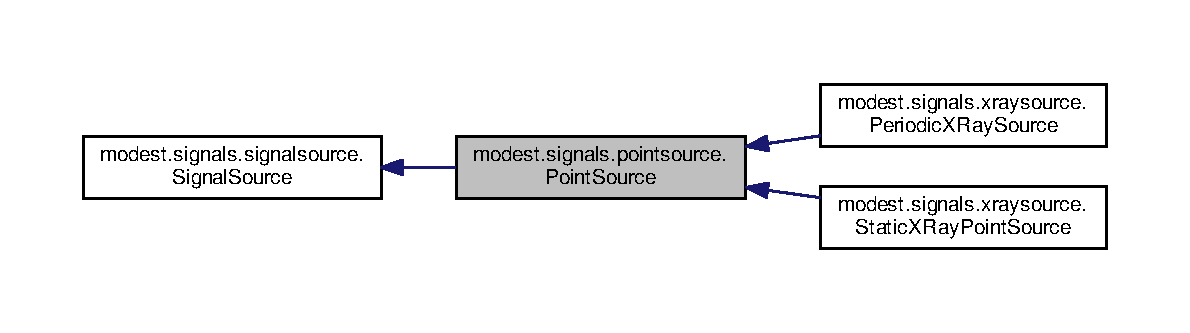
\includegraphics[width=223pt]{classmodest_1_1signals_1_1pointsource_1_1PointSource__inherit__graph}
\end{center}
\end{figure}


Collaboration diagram for modest.\+signals.\+pointsource.\+Point\+Source\+:\nopagebreak
\begin{figure}[H]
\begin{center}
\leavevmode
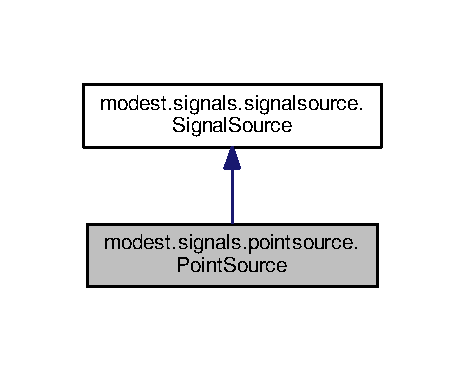
\includegraphics[width=223pt]{classmodest_1_1signals_1_1pointsource_1_1PointSource__coll__graph}
\end{center}
\end{figure}
\subsection*{Public Member Functions}
\begin{DoxyCompactItemize}
\item 
def \hyperlink{classmodest_1_1signals_1_1pointsource_1_1PointSource_a32143ad5b008b5e763fb2bb4cd984924}{\+\_\+\+\_\+init\+\_\+\+\_\+} (self, RA, D\+EC, \hyperlink{classmodest_1_1signals_1_1pointsource_1_1PointSource_a0924a2233bb4fd23e50d024e4f1b048e}{attitude\+State\+Name}=\textquotesingle{}attitude\textquotesingle{})
\item 
def \hyperlink{classmodest_1_1signals_1_1pointsource_1_1PointSource_a295eb1a487e18c77029585ac2785db80}{Ra\+Dec} (self)
\item 
def \hyperlink{classmodest_1_1signals_1_1pointsource_1_1PointSource_aa51308fcb654e7183d332ed824965397}{unit\+Vec} (self, \hyperlink{classmodest_1_1signals_1_1pointsource_1_1PointSource_a295eb1a487e18c77029585ac2785db80}{Ra\+Dec})
\item 
def \hyperlink{classmodest_1_1signals_1_1pointsource_1_1PointSource_a8bdf640e312bbf3a56efd0e89d496361}{compute\+Association\+Probability} (self, measurement, state\+Dict, validation\+Threshold=0)
\item 
def \hyperlink{classmodest_1_1signals_1_1signalsource_1_1SignalSource_a9a64c6a9c2954f6ad61e4ca3518ea8ab}{signal\+ID} (self)
\end{DoxyCompactItemize}
\subsection*{Public Attributes}
\begin{DoxyCompactItemize}
\item 
\hyperlink{classmodest_1_1signals_1_1pointsource_1_1PointSource_a0924a2233bb4fd23e50d024e4f1b048e}{attitude\+State\+Name}
\end{DoxyCompactItemize}
\subsection*{Static Public Attributes}
\begin{DoxyCompactItemize}
\item 
int \hyperlink{classmodest_1_1signals_1_1signalsource_1_1SignalSource_a453eafb550b551adbec0903deb63dfce}{next\+Signal\+ID} = 0
\end{DoxyCompactItemize}
\subsection*{Private Attributes}
\begin{DoxyCompactItemize}
\item 
\hyperlink{classmodest_1_1signals_1_1pointsource_1_1PointSource_a387c0a61a8be5dadf9bd746c0558abbb}{\+\_\+\+\_\+\+R\+A\+\_\+\+\_\+}
\item 
\hyperlink{classmodest_1_1signals_1_1pointsource_1_1PointSource_a72742886f580c8c14109e9c338cf5d1b}{\+\_\+\+\_\+\+D\+E\+C\+\_\+\+\_\+}
\item 
\hyperlink{classmodest_1_1signals_1_1pointsource_1_1PointSource_a2f5e54ab758c3b6126f7a5b1785520ff}{\+\_\+\+\_\+\+Ra\+Dec\+\_\+\+\_\+}
\end{DoxyCompactItemize}


\subsection{Detailed Description}


Definition at line 6 of file pointsource.\+py.



\subsection{Constructor \& Destructor Documentation}
\index{modest\+::signals\+::pointsource\+::\+Point\+Source@{modest\+::signals\+::pointsource\+::\+Point\+Source}!\+\_\+\+\_\+init\+\_\+\+\_\+@{\+\_\+\+\_\+init\+\_\+\+\_\+}}
\index{\+\_\+\+\_\+init\+\_\+\+\_\+@{\+\_\+\+\_\+init\+\_\+\+\_\+}!modest\+::signals\+::pointsource\+::\+Point\+Source@{modest\+::signals\+::pointsource\+::\+Point\+Source}}
\subsubsection[{\texorpdfstring{\+\_\+\+\_\+init\+\_\+\+\_\+(self, R\+A, D\+E\+C, attitude\+State\+Name=\textquotesingle{}attitude\textquotesingle{})}{__init__(self, RA, DEC, attitudeStateName='attitude')}}]{\setlength{\rightskip}{0pt plus 5cm}def modest.\+signals.\+pointsource.\+Point\+Source.\+\_\+\+\_\+init\+\_\+\+\_\+ (
\begin{DoxyParamCaption}
\item[{}]{self, }
\item[{}]{RA, }
\item[{}]{D\+EC, }
\item[{}]{attitude\+State\+Name = {\ttfamily \textquotesingle{}attitude\textquotesingle{}}}
\end{DoxyParamCaption}
)}\hypertarget{classmodest_1_1signals_1_1pointsource_1_1PointSource_a32143ad5b008b5e763fb2bb4cd984924}{}\label{classmodest_1_1signals_1_1pointsource_1_1PointSource_a32143ad5b008b5e763fb2bb4cd984924}


Definition at line 12 of file pointsource.\+py.



\subsection{Member Function Documentation}
\index{modest\+::signals\+::pointsource\+::\+Point\+Source@{modest\+::signals\+::pointsource\+::\+Point\+Source}!compute\+Association\+Probability@{compute\+Association\+Probability}}
\index{compute\+Association\+Probability@{compute\+Association\+Probability}!modest\+::signals\+::pointsource\+::\+Point\+Source@{modest\+::signals\+::pointsource\+::\+Point\+Source}}
\subsubsection[{\texorpdfstring{compute\+Association\+Probability(self, measurement, state\+Dict, validation\+Threshold=0)}{computeAssociationProbability(self, measurement, stateDict, validationThreshold=0)}}]{\setlength{\rightskip}{0pt plus 5cm}def modest.\+signals.\+pointsource.\+Point\+Source.\+compute\+Association\+Probability (
\begin{DoxyParamCaption}
\item[{}]{self, }
\item[{}]{measurement, }
\item[{}]{state\+Dict, }
\item[{}]{validation\+Threshold = {\ttfamily 0}}
\end{DoxyParamCaption}
)}\hypertarget{classmodest_1_1signals_1_1pointsource_1_1PointSource_a8bdf640e312bbf3a56efd0e89d496361}{}\label{classmodest_1_1signals_1_1pointsource_1_1PointSource_a8bdf640e312bbf3a56efd0e89d496361}


Definition at line 39 of file pointsource.\+py.

\index{modest\+::signals\+::pointsource\+::\+Point\+Source@{modest\+::signals\+::pointsource\+::\+Point\+Source}!Ra\+Dec@{Ra\+Dec}}
\index{Ra\+Dec@{Ra\+Dec}!modest\+::signals\+::pointsource\+::\+Point\+Source@{modest\+::signals\+::pointsource\+::\+Point\+Source}}
\subsubsection[{\texorpdfstring{Ra\+Dec(self)}{RaDec(self)}}]{\setlength{\rightskip}{0pt plus 5cm}def modest.\+signals.\+pointsource.\+Point\+Source.\+Ra\+Dec (
\begin{DoxyParamCaption}
\item[{}]{self}
\end{DoxyParamCaption}
)}\hypertarget{classmodest_1_1signals_1_1pointsource_1_1PointSource_a295eb1a487e18c77029585ac2785db80}{}\label{classmodest_1_1signals_1_1pointsource_1_1PointSource_a295eb1a487e18c77029585ac2785db80}


Definition at line 21 of file pointsource.\+py.

\index{modest\+::signals\+::pointsource\+::\+Point\+Source@{modest\+::signals\+::pointsource\+::\+Point\+Source}!signal\+ID@{signal\+ID}}
\index{signal\+ID@{signal\+ID}!modest\+::signals\+::pointsource\+::\+Point\+Source@{modest\+::signals\+::pointsource\+::\+Point\+Source}}
\subsubsection[{\texorpdfstring{signal\+I\+D(self)}{signalID(self)}}]{\setlength{\rightskip}{0pt plus 5cm}def modest.\+signals.\+signalsource.\+Signal\+Source.\+signal\+ID (
\begin{DoxyParamCaption}
\item[{}]{self}
\end{DoxyParamCaption}
)\hspace{0.3cm}{\ttfamily [inherited]}}\hypertarget{classmodest_1_1signals_1_1signalsource_1_1SignalSource_a9a64c6a9c2954f6ad61e4ca3518ea8ab}{}\label{classmodest_1_1signals_1_1signalsource_1_1SignalSource_a9a64c6a9c2954f6ad61e4ca3518ea8ab}


Definition at line 14 of file signalsource.\+py.

\index{modest\+::signals\+::pointsource\+::\+Point\+Source@{modest\+::signals\+::pointsource\+::\+Point\+Source}!unit\+Vec@{unit\+Vec}}
\index{unit\+Vec@{unit\+Vec}!modest\+::signals\+::pointsource\+::\+Point\+Source@{modest\+::signals\+::pointsource\+::\+Point\+Source}}
\subsubsection[{\texorpdfstring{unit\+Vec(self, Ra\+Dec)}{unitVec(self, RaDec)}}]{\setlength{\rightskip}{0pt plus 5cm}def modest.\+signals.\+pointsource.\+Point\+Source.\+unit\+Vec (
\begin{DoxyParamCaption}
\item[{}]{self, }
\item[{}]{Ra\+Dec}
\end{DoxyParamCaption}
)}\hypertarget{classmodest_1_1signals_1_1pointsource_1_1PointSource_aa51308fcb654e7183d332ed824965397}{}\label{classmodest_1_1signals_1_1pointsource_1_1PointSource_aa51308fcb654e7183d332ed824965397}


Definition at line 26 of file pointsource.\+py.



\subsection{Member Data Documentation}
\index{modest\+::signals\+::pointsource\+::\+Point\+Source@{modest\+::signals\+::pointsource\+::\+Point\+Source}!\+\_\+\+\_\+\+D\+E\+C\+\_\+\+\_\+@{\+\_\+\+\_\+\+D\+E\+C\+\_\+\+\_\+}}
\index{\+\_\+\+\_\+\+D\+E\+C\+\_\+\+\_\+@{\+\_\+\+\_\+\+D\+E\+C\+\_\+\+\_\+}!modest\+::signals\+::pointsource\+::\+Point\+Source@{modest\+::signals\+::pointsource\+::\+Point\+Source}}
\subsubsection[{\texorpdfstring{\+\_\+\+\_\+\+D\+E\+C\+\_\+\+\_\+}{__DEC__}}]{\setlength{\rightskip}{0pt plus 5cm}modest.\+signals.\+pointsource.\+Point\+Source.\+\_\+\+\_\+\+D\+E\+C\+\_\+\+\_\+\hspace{0.3cm}{\ttfamily [private]}}\hypertarget{classmodest_1_1signals_1_1pointsource_1_1PointSource_a72742886f580c8c14109e9c338cf5d1b}{}\label{classmodest_1_1signals_1_1pointsource_1_1PointSource_a72742886f580c8c14109e9c338cf5d1b}


Definition at line 15 of file pointsource.\+py.

\index{modest\+::signals\+::pointsource\+::\+Point\+Source@{modest\+::signals\+::pointsource\+::\+Point\+Source}!\+\_\+\+\_\+\+R\+A\+\_\+\+\_\+@{\+\_\+\+\_\+\+R\+A\+\_\+\+\_\+}}
\index{\+\_\+\+\_\+\+R\+A\+\_\+\+\_\+@{\+\_\+\+\_\+\+R\+A\+\_\+\+\_\+}!modest\+::signals\+::pointsource\+::\+Point\+Source@{modest\+::signals\+::pointsource\+::\+Point\+Source}}
\subsubsection[{\texorpdfstring{\+\_\+\+\_\+\+R\+A\+\_\+\+\_\+}{__RA__}}]{\setlength{\rightskip}{0pt plus 5cm}modest.\+signals.\+pointsource.\+Point\+Source.\+\_\+\+\_\+\+R\+A\+\_\+\+\_\+\hspace{0.3cm}{\ttfamily [private]}}\hypertarget{classmodest_1_1signals_1_1pointsource_1_1PointSource_a387c0a61a8be5dadf9bd746c0558abbb}{}\label{classmodest_1_1signals_1_1pointsource_1_1PointSource_a387c0a61a8be5dadf9bd746c0558abbb}


Definition at line 14 of file pointsource.\+py.

\index{modest\+::signals\+::pointsource\+::\+Point\+Source@{modest\+::signals\+::pointsource\+::\+Point\+Source}!\+\_\+\+\_\+\+Ra\+Dec\+\_\+\+\_\+@{\+\_\+\+\_\+\+Ra\+Dec\+\_\+\+\_\+}}
\index{\+\_\+\+\_\+\+Ra\+Dec\+\_\+\+\_\+@{\+\_\+\+\_\+\+Ra\+Dec\+\_\+\+\_\+}!modest\+::signals\+::pointsource\+::\+Point\+Source@{modest\+::signals\+::pointsource\+::\+Point\+Source}}
\subsubsection[{\texorpdfstring{\+\_\+\+\_\+\+Ra\+Dec\+\_\+\+\_\+}{__RaDec__}}]{\setlength{\rightskip}{0pt plus 5cm}modest.\+signals.\+pointsource.\+Point\+Source.\+\_\+\+\_\+\+Ra\+Dec\+\_\+\+\_\+\hspace{0.3cm}{\ttfamily [private]}}\hypertarget{classmodest_1_1signals_1_1pointsource_1_1PointSource_a2f5e54ab758c3b6126f7a5b1785520ff}{}\label{classmodest_1_1signals_1_1pointsource_1_1PointSource_a2f5e54ab758c3b6126f7a5b1785520ff}


Definition at line 16 of file pointsource.\+py.

\index{modest\+::signals\+::pointsource\+::\+Point\+Source@{modest\+::signals\+::pointsource\+::\+Point\+Source}!attitude\+State\+Name@{attitude\+State\+Name}}
\index{attitude\+State\+Name@{attitude\+State\+Name}!modest\+::signals\+::pointsource\+::\+Point\+Source@{modest\+::signals\+::pointsource\+::\+Point\+Source}}
\subsubsection[{\texorpdfstring{attitude\+State\+Name}{attitudeStateName}}]{\setlength{\rightskip}{0pt plus 5cm}modest.\+signals.\+pointsource.\+Point\+Source.\+attitude\+State\+Name}\hypertarget{classmodest_1_1signals_1_1pointsource_1_1PointSource_a0924a2233bb4fd23e50d024e4f1b048e}{}\label{classmodest_1_1signals_1_1pointsource_1_1PointSource_a0924a2233bb4fd23e50d024e4f1b048e}


Definition at line 17 of file pointsource.\+py.

\index{modest\+::signals\+::pointsource\+::\+Point\+Source@{modest\+::signals\+::pointsource\+::\+Point\+Source}!next\+Signal\+ID@{next\+Signal\+ID}}
\index{next\+Signal\+ID@{next\+Signal\+ID}!modest\+::signals\+::pointsource\+::\+Point\+Source@{modest\+::signals\+::pointsource\+::\+Point\+Source}}
\subsubsection[{\texorpdfstring{next\+Signal\+ID}{nextSignalID}}]{\setlength{\rightskip}{0pt plus 5cm}int modest.\+signals.\+signalsource.\+Signal\+Source.\+next\+Signal\+ID = 0\hspace{0.3cm}{\ttfamily [static]}, {\ttfamily [inherited]}}\hypertarget{classmodest_1_1signals_1_1signalsource_1_1SignalSource_a453eafb550b551adbec0903deb63dfce}{}\label{classmodest_1_1signals_1_1signalsource_1_1SignalSource_a453eafb550b551adbec0903deb63dfce}


Definition at line 5 of file signalsource.\+py.



The documentation for this class was generated from the following file\+:\begin{DoxyCompactItemize}
\item 
modest/signals/\hyperlink{pointsource_8py}{pointsource.\+py}\end{DoxyCompactItemize}

\hypertarget{classmodest_1_1signals_1_1poissonsource_1_1PoissonSource}{}\section{modest.\+signals.\+poissonsource.\+Poisson\+Source Class Reference}
\label{classmodest_1_1signals_1_1poissonsource_1_1PoissonSource}\index{modest.\+signals.\+poissonsource.\+Poisson\+Source@{modest.\+signals.\+poissonsource.\+Poisson\+Source}}


Inheritance diagram for modest.\+signals.\+poissonsource.\+Poisson\+Source\+:
\nopagebreak
\begin{figure}[H]
\begin{center}
\leavevmode
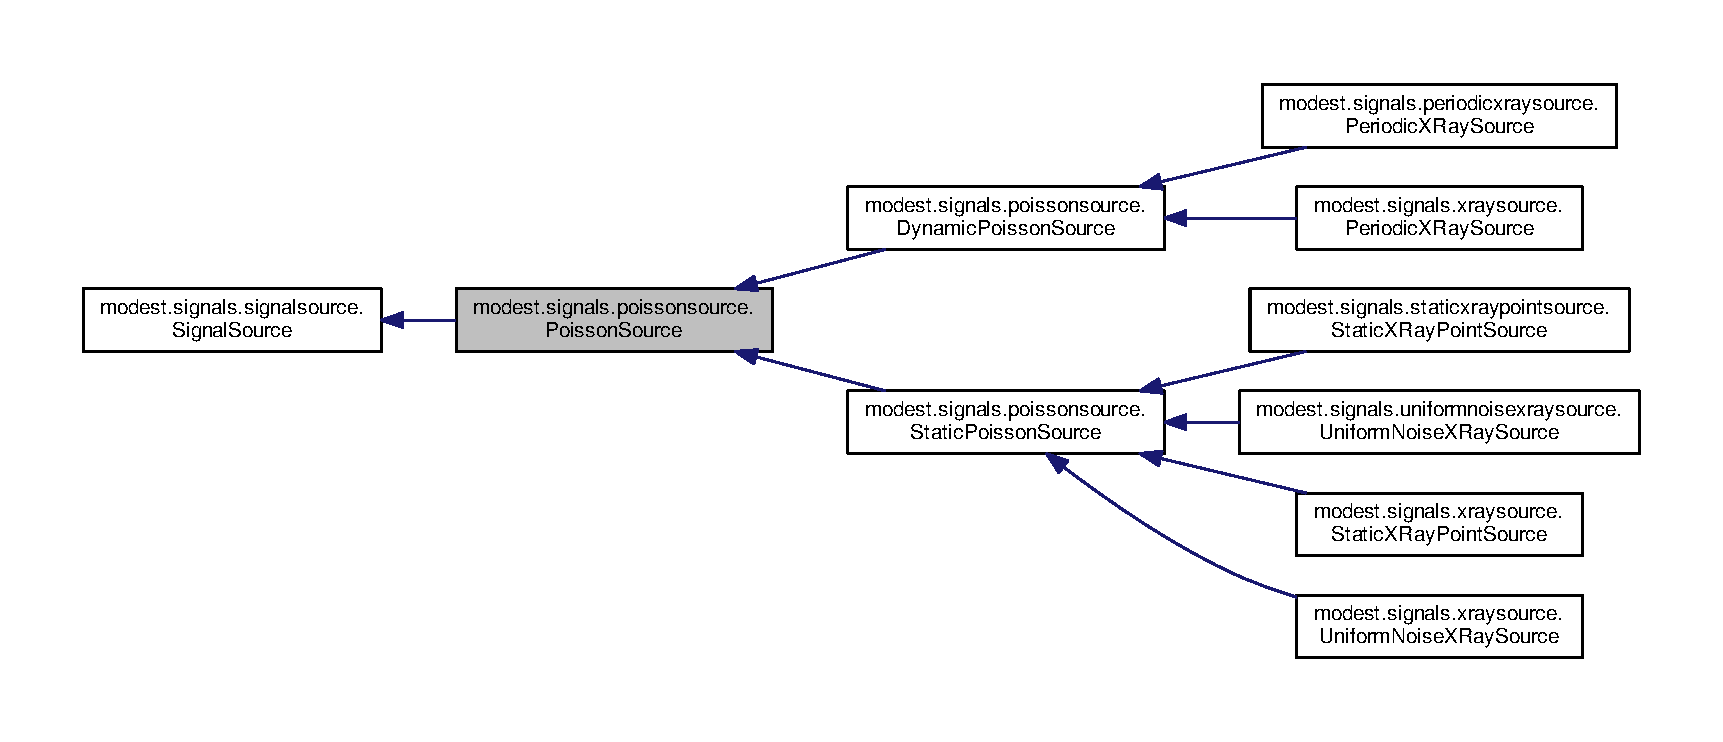
\includegraphics[width=350pt]{classmodest_1_1signals_1_1poissonsource_1_1PoissonSource__inherit__graph}
\end{center}
\end{figure}


Collaboration diagram for modest.\+signals.\+poissonsource.\+Poisson\+Source\+:\nopagebreak
\begin{figure}[H]
\begin{center}
\leavevmode
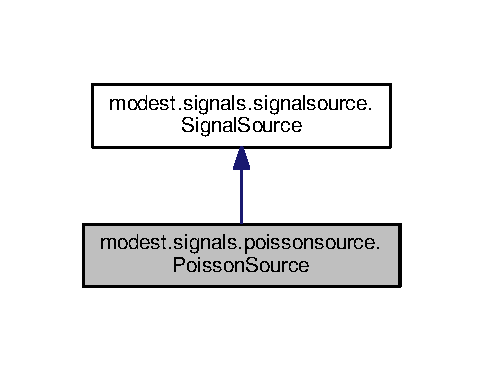
\includegraphics[width=232pt]{classmodest_1_1signals_1_1poissonsource_1_1PoissonSource__coll__graph}
\end{center}
\end{figure}
\subsection*{Public Member Functions}
\begin{DoxyCompactItemize}
\item 
def \hyperlink{classmodest_1_1signals_1_1poissonsource_1_1PoissonSource_ac1abf56553d7e26d2e93b2b3c2c42d97}{\+\_\+\+\_\+init\+\_\+\+\_\+} (self, \hyperlink{classmodest_1_1signals_1_1poissonsource_1_1PoissonSource_a6f2c657ad936b921715d826ac74f7fe5}{flux}, start\+Time=0)
\item 
def \hyperlink{classmodest_1_1signals_1_1poissonsource_1_1PoissonSource_a2f8a73e6f51cbdcd0f1e646d6f4d4574}{compute\+Association\+Probability} (self, current\+Flux, measurement)
\item 
def \hyperlink{classmodest_1_1signals_1_1signalsource_1_1SignalSource_a9a64c6a9c2954f6ad61e4ca3518ea8ab}{signal\+ID} (self)
\item 
def \hyperlink{classmodest_1_1signals_1_1signalsource_1_1SignalSource_a3d32dbed840ea9ac775b226f0a654831}{compute\+Association\+Probability} (self, measurement, state\+Dict, validation\+Threshold=0)
\end{DoxyCompactItemize}
\subsection*{Public Attributes}
\begin{DoxyCompactItemize}
\item 
\hyperlink{classmodest_1_1signals_1_1poissonsource_1_1PoissonSource_a34395fc83bd8743a0a5ee69f9392a606}{last\+Time}
\item 
\hyperlink{classmodest_1_1signals_1_1poissonsource_1_1PoissonSource_a6f2c657ad936b921715d826ac74f7fe5}{flux}
\end{DoxyCompactItemize}
\subsection*{Static Public Attributes}
\begin{DoxyCompactItemize}
\item 
int \hyperlink{classmodest_1_1signals_1_1signalsource_1_1SignalSource_a453eafb550b551adbec0903deb63dfce}{next\+Signal\+ID} = 0
\end{DoxyCompactItemize}


\subsection{Detailed Description}


Definition at line 8 of file poissonsource.\+py.



\subsection{Constructor \& Destructor Documentation}
\index{modest\+::signals\+::poissonsource\+::\+Poisson\+Source@{modest\+::signals\+::poissonsource\+::\+Poisson\+Source}!\+\_\+\+\_\+init\+\_\+\+\_\+@{\+\_\+\+\_\+init\+\_\+\+\_\+}}
\index{\+\_\+\+\_\+init\+\_\+\+\_\+@{\+\_\+\+\_\+init\+\_\+\+\_\+}!modest\+::signals\+::poissonsource\+::\+Poisson\+Source@{modest\+::signals\+::poissonsource\+::\+Poisson\+Source}}
\subsubsection[{\texorpdfstring{\+\_\+\+\_\+init\+\_\+\+\_\+(self, flux, start\+Time=0)}{__init__(self, flux, startTime=0)}}]{\setlength{\rightskip}{0pt plus 5cm}def modest.\+signals.\+poissonsource.\+Poisson\+Source.\+\_\+\+\_\+init\+\_\+\+\_\+ (
\begin{DoxyParamCaption}
\item[{}]{self, }
\item[{}]{flux, }
\item[{}]{start\+Time = {\ttfamily 0}}
\end{DoxyParamCaption}
)}\hypertarget{classmodest_1_1signals_1_1poissonsource_1_1PoissonSource_ac1abf56553d7e26d2e93b2b3c2c42d97}{}\label{classmodest_1_1signals_1_1poissonsource_1_1PoissonSource_ac1abf56553d7e26d2e93b2b3c2c42d97}


Definition at line 13 of file poissonsource.\+py.



\subsection{Member Function Documentation}
\index{modest\+::signals\+::poissonsource\+::\+Poisson\+Source@{modest\+::signals\+::poissonsource\+::\+Poisson\+Source}!compute\+Association\+Probability@{compute\+Association\+Probability}}
\index{compute\+Association\+Probability@{compute\+Association\+Probability}!modest\+::signals\+::poissonsource\+::\+Poisson\+Source@{modest\+::signals\+::poissonsource\+::\+Poisson\+Source}}
\subsubsection[{\texorpdfstring{compute\+Association\+Probability(self, current\+Flux, measurement)}{computeAssociationProbability(self, currentFlux, measurement)}}]{\setlength{\rightskip}{0pt plus 5cm}def modest.\+signals.\+poissonsource.\+Poisson\+Source.\+compute\+Association\+Probability (
\begin{DoxyParamCaption}
\item[{}]{self, }
\item[{}]{current\+Flux, }
\item[{}]{measurement}
\end{DoxyParamCaption}
)}\hypertarget{classmodest_1_1signals_1_1poissonsource_1_1PoissonSource_a2f8a73e6f51cbdcd0f1e646d6f4d4574}{}\label{classmodest_1_1signals_1_1poissonsource_1_1PoissonSource_a2f8a73e6f51cbdcd0f1e646d6f4d4574}


Definition at line 23 of file poissonsource.\+py.

\index{modest\+::signals\+::poissonsource\+::\+Poisson\+Source@{modest\+::signals\+::poissonsource\+::\+Poisson\+Source}!compute\+Association\+Probability@{compute\+Association\+Probability}}
\index{compute\+Association\+Probability@{compute\+Association\+Probability}!modest\+::signals\+::poissonsource\+::\+Poisson\+Source@{modest\+::signals\+::poissonsource\+::\+Poisson\+Source}}
\subsubsection[{\texorpdfstring{compute\+Association\+Probability(self, measurement, state\+Dict, validation\+Threshold=0)}{computeAssociationProbability(self, measurement, stateDict, validationThreshold=0)}}]{\setlength{\rightskip}{0pt plus 5cm}def modest.\+signals.\+signalsource.\+Signal\+Source.\+compute\+Association\+Probability (
\begin{DoxyParamCaption}
\item[{}]{self, }
\item[{}]{measurement, }
\item[{}]{state\+Dict, }
\item[{}]{validation\+Threshold = {\ttfamily 0}}
\end{DoxyParamCaption}
)\hspace{0.3cm}{\ttfamily [inherited]}}\hypertarget{classmodest_1_1signals_1_1signalsource_1_1SignalSource_a3d32dbed840ea9ac775b226f0a654831}{}\label{classmodest_1_1signals_1_1signalsource_1_1SignalSource_a3d32dbed840ea9ac775b226f0a654831}


Definition at line 26 of file signalsource.\+py.

\index{modest\+::signals\+::poissonsource\+::\+Poisson\+Source@{modest\+::signals\+::poissonsource\+::\+Poisson\+Source}!signal\+ID@{signal\+ID}}
\index{signal\+ID@{signal\+ID}!modest\+::signals\+::poissonsource\+::\+Poisson\+Source@{modest\+::signals\+::poissonsource\+::\+Poisson\+Source}}
\subsubsection[{\texorpdfstring{signal\+I\+D(self)}{signalID(self)}}]{\setlength{\rightskip}{0pt plus 5cm}def modest.\+signals.\+signalsource.\+Signal\+Source.\+signal\+ID (
\begin{DoxyParamCaption}
\item[{}]{self}
\end{DoxyParamCaption}
)\hspace{0.3cm}{\ttfamily [inherited]}}\hypertarget{classmodest_1_1signals_1_1signalsource_1_1SignalSource_a9a64c6a9c2954f6ad61e4ca3518ea8ab}{}\label{classmodest_1_1signals_1_1signalsource_1_1SignalSource_a9a64c6a9c2954f6ad61e4ca3518ea8ab}


Definition at line 17 of file signalsource.\+py.



\subsection{Member Data Documentation}
\index{modest\+::signals\+::poissonsource\+::\+Poisson\+Source@{modest\+::signals\+::poissonsource\+::\+Poisson\+Source}!flux@{flux}}
\index{flux@{flux}!modest\+::signals\+::poissonsource\+::\+Poisson\+Source@{modest\+::signals\+::poissonsource\+::\+Poisson\+Source}}
\subsubsection[{\texorpdfstring{flux}{flux}}]{\setlength{\rightskip}{0pt plus 5cm}modest.\+signals.\+poissonsource.\+Poisson\+Source.\+flux}\hypertarget{classmodest_1_1signals_1_1poissonsource_1_1PoissonSource_a6f2c657ad936b921715d826ac74f7fe5}{}\label{classmodest_1_1signals_1_1poissonsource_1_1PoissonSource_a6f2c657ad936b921715d826ac74f7fe5}


Definition at line 16 of file poissonsource.\+py.

\index{modest\+::signals\+::poissonsource\+::\+Poisson\+Source@{modest\+::signals\+::poissonsource\+::\+Poisson\+Source}!last\+Time@{last\+Time}}
\index{last\+Time@{last\+Time}!modest\+::signals\+::poissonsource\+::\+Poisson\+Source@{modest\+::signals\+::poissonsource\+::\+Poisson\+Source}}
\subsubsection[{\texorpdfstring{last\+Time}{lastTime}}]{\setlength{\rightskip}{0pt plus 5cm}modest.\+signals.\+poissonsource.\+Poisson\+Source.\+last\+Time}\hypertarget{classmodest_1_1signals_1_1poissonsource_1_1PoissonSource_a34395fc83bd8743a0a5ee69f9392a606}{}\label{classmodest_1_1signals_1_1poissonsource_1_1PoissonSource_a34395fc83bd8743a0a5ee69f9392a606}


Definition at line 15 of file poissonsource.\+py.

\index{modest\+::signals\+::poissonsource\+::\+Poisson\+Source@{modest\+::signals\+::poissonsource\+::\+Poisson\+Source}!next\+Signal\+ID@{next\+Signal\+ID}}
\index{next\+Signal\+ID@{next\+Signal\+ID}!modest\+::signals\+::poissonsource\+::\+Poisson\+Source@{modest\+::signals\+::poissonsource\+::\+Poisson\+Source}}
\subsubsection[{\texorpdfstring{next\+Signal\+ID}{nextSignalID}}]{\setlength{\rightskip}{0pt plus 5cm}int modest.\+signals.\+signalsource.\+Signal\+Source.\+next\+Signal\+ID = 0\hspace{0.3cm}{\ttfamily [static]}, {\ttfamily [inherited]}}\hypertarget{classmodest_1_1signals_1_1signalsource_1_1SignalSource_a453eafb550b551adbec0903deb63dfce}{}\label{classmodest_1_1signals_1_1signalsource_1_1SignalSource_a453eafb550b551adbec0903deb63dfce}


Definition at line 8 of file signalsource.\+py.



The documentation for this class was generated from the following file\+:\begin{DoxyCompactItemize}
\item 
modest/signals/\hyperlink{poissonsource_8py}{poissonsource.\+py}\end{DoxyCompactItemize}

\hypertarget{classmodest_1_1signals_1_1signalsource_1_1SignalSource}{}\section{modest.\+signals.\+signalsource.\+Signal\+Source Class Reference}
\label{classmodest_1_1signals_1_1signalsource_1_1SignalSource}\index{modest.\+signals.\+signalsource.\+Signal\+Source@{modest.\+signals.\+signalsource.\+Signal\+Source}}


Inheritance diagram for modest.\+signals.\+signalsource.\+Signal\+Source\+:
\nopagebreak
\begin{figure}[H]
\begin{center}
\leavevmode
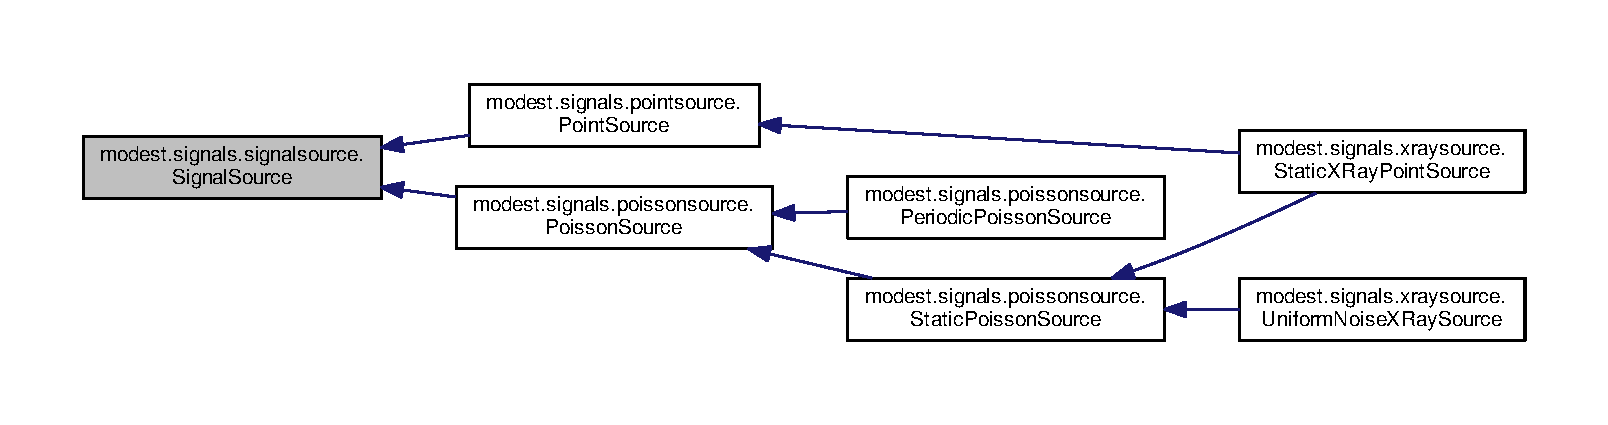
\includegraphics[width=350pt]{classmodest_1_1signals_1_1signalsource_1_1SignalSource__inherit__graph}
\end{center}
\end{figure}
\subsection*{Public Member Functions}
\begin{DoxyCompactItemize}
\item 
def \hyperlink{classmodest_1_1signals_1_1signalsource_1_1SignalSource_abc71be8fa60c2431ee68d4b7752684f0}{\+\_\+\+\_\+init\+\_\+\+\_\+} (self)
\item 
def \hyperlink{classmodest_1_1signals_1_1signalsource_1_1SignalSource_a9a64c6a9c2954f6ad61e4ca3518ea8ab}{signal\+ID} (self)
\item 
def \hyperlink{classmodest_1_1signals_1_1signalsource_1_1SignalSource_a3d32dbed840ea9ac775b226f0a654831}{compute\+Association\+Probability} (self, measurement, state\+Dict, validation\+Threshold=0)
\end{DoxyCompactItemize}
\subsection*{Static Public Attributes}
\begin{DoxyCompactItemize}
\item 
int \hyperlink{classmodest_1_1signals_1_1signalsource_1_1SignalSource_a453eafb550b551adbec0903deb63dfce}{next\+Signal\+ID} = 0
\end{DoxyCompactItemize}
\subsection*{Private Attributes}
\begin{DoxyCompactItemize}
\item 
\hyperlink{classmodest_1_1signals_1_1signalsource_1_1SignalSource_a8b8d7f422fe4de0e2f0add245c05b3c1}{\+\_\+\+\_\+signal\+I\+D\+\_\+\+\_\+}
\end{DoxyCompactItemize}
\subsection*{Static Private Attributes}
\begin{DoxyCompactItemize}
\item 
\hyperlink{classmodest_1_1signals_1_1signalsource_1_1SignalSource_a07d7658d1b008499bcdf05c718638160}{\+\_\+\+\_\+metaclass\+\_\+\+\_\+} = A\+B\+C\+Meta
\end{DoxyCompactItemize}


\subsection{Detailed Description}


Definition at line 6 of file signalsource.\+py.



\subsection{Constructor \& Destructor Documentation}
\index{modest\+::signals\+::signalsource\+::\+Signal\+Source@{modest\+::signals\+::signalsource\+::\+Signal\+Source}!\+\_\+\+\_\+init\+\_\+\+\_\+@{\+\_\+\+\_\+init\+\_\+\+\_\+}}
\index{\+\_\+\+\_\+init\+\_\+\+\_\+@{\+\_\+\+\_\+init\+\_\+\+\_\+}!modest\+::signals\+::signalsource\+::\+Signal\+Source@{modest\+::signals\+::signalsource\+::\+Signal\+Source}}
\subsubsection[{\texorpdfstring{\+\_\+\+\_\+init\+\_\+\+\_\+(self)}{__init__(self)}}]{\setlength{\rightskip}{0pt plus 5cm}def modest.\+signals.\+signalsource.\+Signal\+Source.\+\_\+\+\_\+init\+\_\+\+\_\+ (
\begin{DoxyParamCaption}
\item[{}]{self}
\end{DoxyParamCaption}
)}\hypertarget{classmodest_1_1signals_1_1signalsource_1_1SignalSource_abc71be8fa60c2431ee68d4b7752684f0}{}\label{classmodest_1_1signals_1_1signalsource_1_1SignalSource_abc71be8fa60c2431ee68d4b7752684f0}


Definition at line 12 of file signalsource.\+py.



\subsection{Member Function Documentation}
\index{modest\+::signals\+::signalsource\+::\+Signal\+Source@{modest\+::signals\+::signalsource\+::\+Signal\+Source}!compute\+Association\+Probability@{compute\+Association\+Probability}}
\index{compute\+Association\+Probability@{compute\+Association\+Probability}!modest\+::signals\+::signalsource\+::\+Signal\+Source@{modest\+::signals\+::signalsource\+::\+Signal\+Source}}
\subsubsection[{\texorpdfstring{compute\+Association\+Probability(self, measurement, state\+Dict, validation\+Threshold=0)}{computeAssociationProbability(self, measurement, stateDict, validationThreshold=0)}}]{\setlength{\rightskip}{0pt plus 5cm}def modest.\+signals.\+signalsource.\+Signal\+Source.\+compute\+Association\+Probability (
\begin{DoxyParamCaption}
\item[{}]{self, }
\item[{}]{measurement, }
\item[{}]{state\+Dict, }
\item[{}]{validation\+Threshold = {\ttfamily 0}}
\end{DoxyParamCaption}
)}\hypertarget{classmodest_1_1signals_1_1signalsource_1_1SignalSource_a3d32dbed840ea9ac775b226f0a654831}{}\label{classmodest_1_1signals_1_1signalsource_1_1SignalSource_a3d32dbed840ea9ac775b226f0a654831}


Definition at line 26 of file signalsource.\+py.

\index{modest\+::signals\+::signalsource\+::\+Signal\+Source@{modest\+::signals\+::signalsource\+::\+Signal\+Source}!signal\+ID@{signal\+ID}}
\index{signal\+ID@{signal\+ID}!modest\+::signals\+::signalsource\+::\+Signal\+Source@{modest\+::signals\+::signalsource\+::\+Signal\+Source}}
\subsubsection[{\texorpdfstring{signal\+I\+D(self)}{signalID(self)}}]{\setlength{\rightskip}{0pt plus 5cm}def modest.\+signals.\+signalsource.\+Signal\+Source.\+signal\+ID (
\begin{DoxyParamCaption}
\item[{}]{self}
\end{DoxyParamCaption}
)}\hypertarget{classmodest_1_1signals_1_1signalsource_1_1SignalSource_a9a64c6a9c2954f6ad61e4ca3518ea8ab}{}\label{classmodest_1_1signals_1_1signalsource_1_1SignalSource_a9a64c6a9c2954f6ad61e4ca3518ea8ab}


Definition at line 17 of file signalsource.\+py.



\subsection{Member Data Documentation}
\index{modest\+::signals\+::signalsource\+::\+Signal\+Source@{modest\+::signals\+::signalsource\+::\+Signal\+Source}!\+\_\+\+\_\+metaclass\+\_\+\+\_\+@{\+\_\+\+\_\+metaclass\+\_\+\+\_\+}}
\index{\+\_\+\+\_\+metaclass\+\_\+\+\_\+@{\+\_\+\+\_\+metaclass\+\_\+\+\_\+}!modest\+::signals\+::signalsource\+::\+Signal\+Source@{modest\+::signals\+::signalsource\+::\+Signal\+Source}}
\subsubsection[{\texorpdfstring{\+\_\+\+\_\+metaclass\+\_\+\+\_\+}{__metaclass__}}]{\setlength{\rightskip}{0pt plus 5cm}modest.\+signals.\+signalsource.\+Signal\+Source.\+\_\+\+\_\+metaclass\+\_\+\+\_\+ = A\+B\+C\+Meta\hspace{0.3cm}{\ttfamily [static]}, {\ttfamily [private]}}\hypertarget{classmodest_1_1signals_1_1signalsource_1_1SignalSource_a07d7658d1b008499bcdf05c718638160}{}\label{classmodest_1_1signals_1_1signalsource_1_1SignalSource_a07d7658d1b008499bcdf05c718638160}


Definition at line 7 of file signalsource.\+py.

\index{modest\+::signals\+::signalsource\+::\+Signal\+Source@{modest\+::signals\+::signalsource\+::\+Signal\+Source}!\+\_\+\+\_\+signal\+I\+D\+\_\+\+\_\+@{\+\_\+\+\_\+signal\+I\+D\+\_\+\+\_\+}}
\index{\+\_\+\+\_\+signal\+I\+D\+\_\+\+\_\+@{\+\_\+\+\_\+signal\+I\+D\+\_\+\+\_\+}!modest\+::signals\+::signalsource\+::\+Signal\+Source@{modest\+::signals\+::signalsource\+::\+Signal\+Source}}
\subsubsection[{\texorpdfstring{\+\_\+\+\_\+signal\+I\+D\+\_\+\+\_\+}{__signalID__}}]{\setlength{\rightskip}{0pt plus 5cm}modest.\+signals.\+signalsource.\+Signal\+Source.\+\_\+\+\_\+signal\+I\+D\+\_\+\+\_\+\hspace{0.3cm}{\ttfamily [private]}}\hypertarget{classmodest_1_1signals_1_1signalsource_1_1SignalSource_a8b8d7f422fe4de0e2f0add245c05b3c1}{}\label{classmodest_1_1signals_1_1signalsource_1_1SignalSource_a8b8d7f422fe4de0e2f0add245c05b3c1}


Definition at line 13 of file signalsource.\+py.

\index{modest\+::signals\+::signalsource\+::\+Signal\+Source@{modest\+::signals\+::signalsource\+::\+Signal\+Source}!next\+Signal\+ID@{next\+Signal\+ID}}
\index{next\+Signal\+ID@{next\+Signal\+ID}!modest\+::signals\+::signalsource\+::\+Signal\+Source@{modest\+::signals\+::signalsource\+::\+Signal\+Source}}
\subsubsection[{\texorpdfstring{next\+Signal\+ID}{nextSignalID}}]{\setlength{\rightskip}{0pt plus 5cm}int modest.\+signals.\+signalsource.\+Signal\+Source.\+next\+Signal\+ID = 0\hspace{0.3cm}{\ttfamily [static]}}\hypertarget{classmodest_1_1signals_1_1signalsource_1_1SignalSource_a453eafb550b551adbec0903deb63dfce}{}\label{classmodest_1_1signals_1_1signalsource_1_1SignalSource_a453eafb550b551adbec0903deb63dfce}


Definition at line 8 of file signalsource.\+py.



The documentation for this class was generated from the following file\+:\begin{DoxyCompactItemize}
\item 
modest/signals/\hyperlink{signalsource_8py}{signalsource.\+py}\end{DoxyCompactItemize}

\hypertarget{classmodest_1_1signals_1_1poissonsource_1_1StaticPoissonSource}{}\section{modest.\+signals.\+poissonsource.\+Static\+Poisson\+Source Class Reference}
\label{classmodest_1_1signals_1_1poissonsource_1_1StaticPoissonSource}\index{modest.\+signals.\+poissonsource.\+Static\+Poisson\+Source@{modest.\+signals.\+poissonsource.\+Static\+Poisson\+Source}}


Inheritance diagram for modest.\+signals.\+poissonsource.\+Static\+Poisson\+Source\+:\nopagebreak
\begin{figure}[H]
\begin{center}
\leavevmode
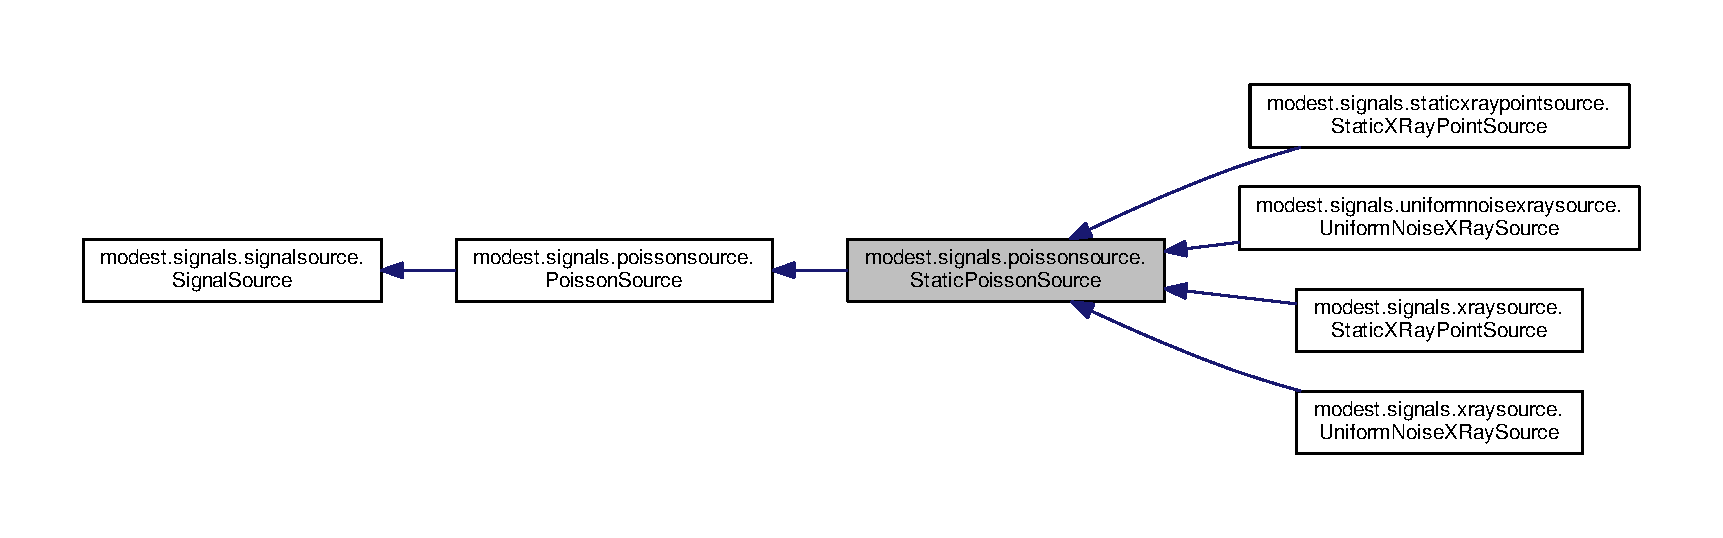
\includegraphics[width=350pt]{classmodest_1_1signals_1_1poissonsource_1_1StaticPoissonSource__inherit__graph}
\end{center}
\end{figure}


Collaboration diagram for modest.\+signals.\+poissonsource.\+Static\+Poisson\+Source\+:\nopagebreak
\begin{figure}[H]
\begin{center}
\leavevmode
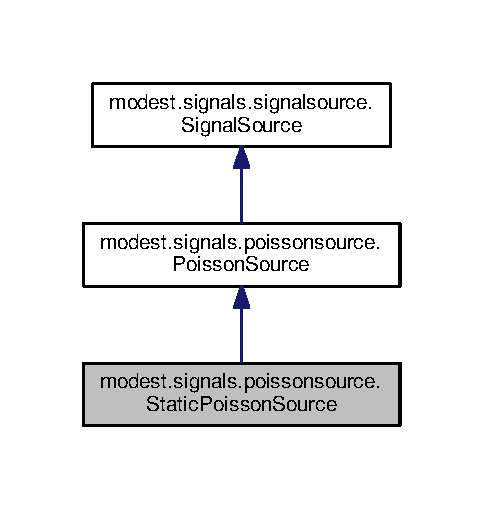
\includegraphics[width=232pt]{classmodest_1_1signals_1_1poissonsource_1_1StaticPoissonSource__coll__graph}
\end{center}
\end{figure}
\subsection*{Public Member Functions}
\begin{DoxyCompactItemize}
\item 
def \hyperlink{classmodest_1_1signals_1_1poissonsource_1_1StaticPoissonSource_aededf35e38bd6e6f148b22911e42e66c}{\+\_\+\+\_\+init\+\_\+\+\_\+} (self, \hyperlink{classmodest_1_1signals_1_1poissonsource_1_1PoissonSource_a6f2c657ad936b921715d826ac74f7fe5}{flux})
\item 
def \hyperlink{classmodest_1_1signals_1_1poissonsource_1_1StaticPoissonSource_a1754d94bff46d97817438bab552afef9}{compute\+Association\+Probability} (self, measurement)
\item 
def \hyperlink{classmodest_1_1signals_1_1poissonsource_1_1PoissonSource_a2f8a73e6f51cbdcd0f1e646d6f4d4574}{compute\+Association\+Probability} (self, current\+Flux, measurement)
\item 
def \hyperlink{classmodest_1_1signals_1_1signalsource_1_1SignalSource_a9a64c6a9c2954f6ad61e4ca3518ea8ab}{signal\+ID} (self)
\end{DoxyCompactItemize}
\subsection*{Public Attributes}
\begin{DoxyCompactItemize}
\item 
\hyperlink{classmodest_1_1signals_1_1poissonsource_1_1PoissonSource_a34395fc83bd8743a0a5ee69f9392a606}{last\+Time}
\item 
\hyperlink{classmodest_1_1signals_1_1poissonsource_1_1PoissonSource_a6f2c657ad936b921715d826ac74f7fe5}{flux}
\end{DoxyCompactItemize}
\subsection*{Static Public Attributes}
\begin{DoxyCompactItemize}
\item 
int \hyperlink{classmodest_1_1signals_1_1signalsource_1_1SignalSource_a453eafb550b551adbec0903deb63dfce}{next\+Signal\+ID} = 0
\end{DoxyCompactItemize}


\subsection{Detailed Description}


Definition at line 27 of file poissonsource.\+py.



\subsection{Constructor \& Destructor Documentation}
\index{modest\+::signals\+::poissonsource\+::\+Static\+Poisson\+Source@{modest\+::signals\+::poissonsource\+::\+Static\+Poisson\+Source}!\+\_\+\+\_\+init\+\_\+\+\_\+@{\+\_\+\+\_\+init\+\_\+\+\_\+}}
\index{\+\_\+\+\_\+init\+\_\+\+\_\+@{\+\_\+\+\_\+init\+\_\+\+\_\+}!modest\+::signals\+::poissonsource\+::\+Static\+Poisson\+Source@{modest\+::signals\+::poissonsource\+::\+Static\+Poisson\+Source}}
\subsubsection[{\texorpdfstring{\+\_\+\+\_\+init\+\_\+\+\_\+(self, flux)}{__init__(self, flux)}}]{\setlength{\rightskip}{0pt plus 5cm}def modest.\+signals.\+poissonsource.\+Static\+Poisson\+Source.\+\_\+\+\_\+init\+\_\+\+\_\+ (
\begin{DoxyParamCaption}
\item[{}]{self, }
\item[{}]{flux}
\end{DoxyParamCaption}
)}\hypertarget{classmodest_1_1signals_1_1poissonsource_1_1StaticPoissonSource_aededf35e38bd6e6f148b22911e42e66c}{}\label{classmodest_1_1signals_1_1poissonsource_1_1StaticPoissonSource_aededf35e38bd6e6f148b22911e42e66c}


Definition at line 31 of file poissonsource.\+py.



\subsection{Member Function Documentation}
\index{modest\+::signals\+::poissonsource\+::\+Static\+Poisson\+Source@{modest\+::signals\+::poissonsource\+::\+Static\+Poisson\+Source}!compute\+Association\+Probability@{compute\+Association\+Probability}}
\index{compute\+Association\+Probability@{compute\+Association\+Probability}!modest\+::signals\+::poissonsource\+::\+Static\+Poisson\+Source@{modest\+::signals\+::poissonsource\+::\+Static\+Poisson\+Source}}
\subsubsection[{\texorpdfstring{compute\+Association\+Probability(self, current\+Flux, measurement)}{computeAssociationProbability(self, currentFlux, measurement)}}]{\setlength{\rightskip}{0pt plus 5cm}def modest.\+signals.\+poissonsource.\+Poisson\+Source.\+compute\+Association\+Probability (
\begin{DoxyParamCaption}
\item[{}]{self, }
\item[{}]{current\+Flux, }
\item[{}]{measurement}
\end{DoxyParamCaption}
)\hspace{0.3cm}{\ttfamily [inherited]}}\hypertarget{classmodest_1_1signals_1_1poissonsource_1_1PoissonSource_a2f8a73e6f51cbdcd0f1e646d6f4d4574}{}\label{classmodest_1_1signals_1_1poissonsource_1_1PoissonSource_a2f8a73e6f51cbdcd0f1e646d6f4d4574}


Definition at line 20 of file poissonsource.\+py.

\index{modest\+::signals\+::poissonsource\+::\+Static\+Poisson\+Source@{modest\+::signals\+::poissonsource\+::\+Static\+Poisson\+Source}!compute\+Association\+Probability@{compute\+Association\+Probability}}
\index{compute\+Association\+Probability@{compute\+Association\+Probability}!modest\+::signals\+::poissonsource\+::\+Static\+Poisson\+Source@{modest\+::signals\+::poissonsource\+::\+Static\+Poisson\+Source}}
\subsubsection[{\texorpdfstring{compute\+Association\+Probability(self, measurement)}{computeAssociationProbability(self, measurement)}}]{\setlength{\rightskip}{0pt plus 5cm}def modest.\+signals.\+poissonsource.\+Static\+Poisson\+Source.\+compute\+Association\+Probability (
\begin{DoxyParamCaption}
\item[{}]{self, }
\item[{}]{measurement}
\end{DoxyParamCaption}
)}\hypertarget{classmodest_1_1signals_1_1poissonsource_1_1StaticPoissonSource_a1754d94bff46d97817438bab552afef9}{}\label{classmodest_1_1signals_1_1poissonsource_1_1StaticPoissonSource_a1754d94bff46d97817438bab552afef9}


Definition at line 37 of file poissonsource.\+py.

\index{modest\+::signals\+::poissonsource\+::\+Static\+Poisson\+Source@{modest\+::signals\+::poissonsource\+::\+Static\+Poisson\+Source}!signal\+ID@{signal\+ID}}
\index{signal\+ID@{signal\+ID}!modest\+::signals\+::poissonsource\+::\+Static\+Poisson\+Source@{modest\+::signals\+::poissonsource\+::\+Static\+Poisson\+Source}}
\subsubsection[{\texorpdfstring{signal\+I\+D(self)}{signalID(self)}}]{\setlength{\rightskip}{0pt plus 5cm}def modest.\+signals.\+signalsource.\+Signal\+Source.\+signal\+ID (
\begin{DoxyParamCaption}
\item[{}]{self}
\end{DoxyParamCaption}
)\hspace{0.3cm}{\ttfamily [inherited]}}\hypertarget{classmodest_1_1signals_1_1signalsource_1_1SignalSource_a9a64c6a9c2954f6ad61e4ca3518ea8ab}{}\label{classmodest_1_1signals_1_1signalsource_1_1SignalSource_a9a64c6a9c2954f6ad61e4ca3518ea8ab}


Definition at line 14 of file signalsource.\+py.



\subsection{Member Data Documentation}
\index{modest\+::signals\+::poissonsource\+::\+Static\+Poisson\+Source@{modest\+::signals\+::poissonsource\+::\+Static\+Poisson\+Source}!flux@{flux}}
\index{flux@{flux}!modest\+::signals\+::poissonsource\+::\+Static\+Poisson\+Source@{modest\+::signals\+::poissonsource\+::\+Static\+Poisson\+Source}}
\subsubsection[{\texorpdfstring{flux}{flux}}]{\setlength{\rightskip}{0pt plus 5cm}modest.\+signals.\+poissonsource.\+Poisson\+Source.\+flux\hspace{0.3cm}{\ttfamily [inherited]}}\hypertarget{classmodest_1_1signals_1_1poissonsource_1_1PoissonSource_a6f2c657ad936b921715d826ac74f7fe5}{}\label{classmodest_1_1signals_1_1poissonsource_1_1PoissonSource_a6f2c657ad936b921715d826ac74f7fe5}


Definition at line 13 of file poissonsource.\+py.

\index{modest\+::signals\+::poissonsource\+::\+Static\+Poisson\+Source@{modest\+::signals\+::poissonsource\+::\+Static\+Poisson\+Source}!last\+Time@{last\+Time}}
\index{last\+Time@{last\+Time}!modest\+::signals\+::poissonsource\+::\+Static\+Poisson\+Source@{modest\+::signals\+::poissonsource\+::\+Static\+Poisson\+Source}}
\subsubsection[{\texorpdfstring{last\+Time}{lastTime}}]{\setlength{\rightskip}{0pt plus 5cm}modest.\+signals.\+poissonsource.\+Poisson\+Source.\+last\+Time\hspace{0.3cm}{\ttfamily [inherited]}}\hypertarget{classmodest_1_1signals_1_1poissonsource_1_1PoissonSource_a34395fc83bd8743a0a5ee69f9392a606}{}\label{classmodest_1_1signals_1_1poissonsource_1_1PoissonSource_a34395fc83bd8743a0a5ee69f9392a606}


Definition at line 12 of file poissonsource.\+py.

\index{modest\+::signals\+::poissonsource\+::\+Static\+Poisson\+Source@{modest\+::signals\+::poissonsource\+::\+Static\+Poisson\+Source}!next\+Signal\+ID@{next\+Signal\+ID}}
\index{next\+Signal\+ID@{next\+Signal\+ID}!modest\+::signals\+::poissonsource\+::\+Static\+Poisson\+Source@{modest\+::signals\+::poissonsource\+::\+Static\+Poisson\+Source}}
\subsubsection[{\texorpdfstring{next\+Signal\+ID}{nextSignalID}}]{\setlength{\rightskip}{0pt plus 5cm}int modest.\+signals.\+signalsource.\+Signal\+Source.\+next\+Signal\+ID = 0\hspace{0.3cm}{\ttfamily [static]}, {\ttfamily [inherited]}}\hypertarget{classmodest_1_1signals_1_1signalsource_1_1SignalSource_a453eafb550b551adbec0903deb63dfce}{}\label{classmodest_1_1signals_1_1signalsource_1_1SignalSource_a453eafb550b551adbec0903deb63dfce}


Definition at line 5 of file signalsource.\+py.



The documentation for this class was generated from the following file\+:\begin{DoxyCompactItemize}
\item 
modest/signals/\hyperlink{poissonsource_8py}{poissonsource.\+py}\end{DoxyCompactItemize}

\hypertarget{classmodest_1_1signals_1_1staticxraypointsource_1_1StaticXRayPointSource}{}\section{modest.\+signals.\+staticxraypointsource.\+Static\+X\+Ray\+Point\+Source Class Reference}
\label{classmodest_1_1signals_1_1staticxraypointsource_1_1StaticXRayPointSource}\index{modest.\+signals.\+staticxraypointsource.\+Static\+X\+Ray\+Point\+Source@{modest.\+signals.\+staticxraypointsource.\+Static\+X\+Ray\+Point\+Source}}


Inheritance diagram for modest.\+signals.\+staticxraypointsource.\+Static\+X\+Ray\+Point\+Source\+:
\nopagebreak
\begin{figure}[H]
\begin{center}
\leavevmode
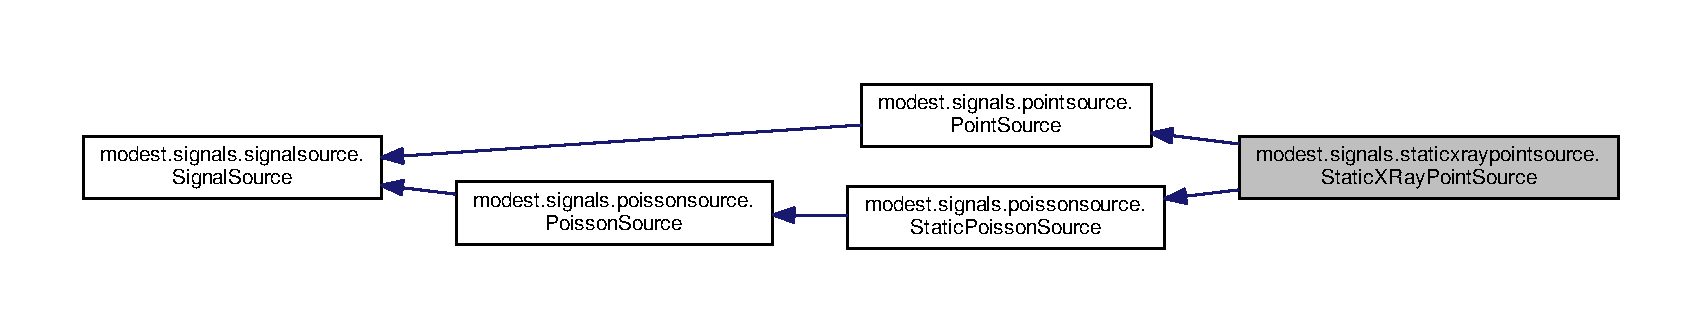
\includegraphics[width=350pt]{classmodest_1_1signals_1_1staticxraypointsource_1_1StaticXRayPointSource__inherit__graph}
\end{center}
\end{figure}


Collaboration diagram for modest.\+signals.\+staticxraypointsource.\+Static\+X\+Ray\+Point\+Source\+:
\nopagebreak
\begin{figure}[H]
\begin{center}
\leavevmode
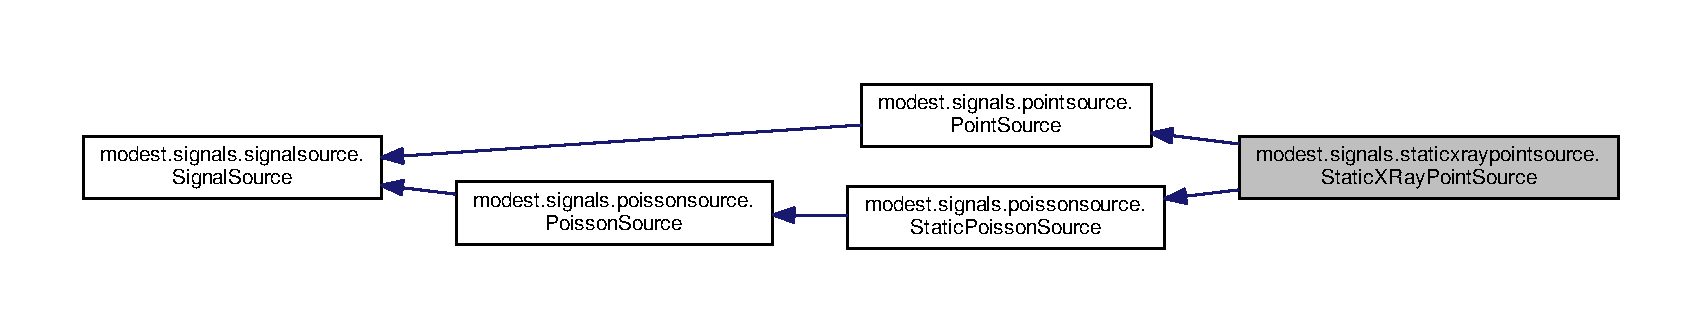
\includegraphics[width=350pt]{classmodest_1_1signals_1_1staticxraypointsource_1_1StaticXRayPointSource__coll__graph}
\end{center}
\end{figure}
\subsection*{Public Member Functions}
\begin{DoxyCompactItemize}
\item 
def \hyperlink{classmodest_1_1signals_1_1staticxraypointsource_1_1StaticXRayPointSource_af3ce1c6b52a940dbbd0e5ac47152bbf4}{\+\_\+\+\_\+init\+\_\+\+\_\+} (self, RA, D\+EC, photon\+Count\+Rate=None, photon\+Energy\+Flux=None, energy\+Range\+KeV=\mbox{[}2, \hyperlink{classmodest_1_1signals_1_1staticxraypointsource_1_1StaticXRayPointSource_a3229134704add2350e5090b2337583f9}{detector\+Area}=1, detector\+F\+OV=np.\+pi, \hyperlink{classmodest_1_1signals_1_1pointsource_1_1PointSource_a0924a2233bb4fd23e50d024e4f1b048e}{attitude\+State\+Name}=\textquotesingle{}attitude\textquotesingle{}, \hyperlink{classmodest_1_1signals_1_1staticxraypointsource_1_1StaticXRayPointSource_adf18ce1f6cf286238d5ae52bd9d3978c}{name}=None, start\+Time=0, \hyperlink{classmodest_1_1signals_1_1pointsource_1_1PointSource_a984b5a75c9e94cb3527707b9ac976f9e}{extent}=0, \hyperlink{classmodest_1_1signals_1_1pointsource_1_1PointSource_ac2dd52c4e1f7e6264c9d59a5ffbc43d1}{use\+Unit\+Vector}=True)
\item 
def \hyperlink{classmodest_1_1signals_1_1staticxraypointsource_1_1StaticXRayPointSource_a323dabf6a6c6b5f52d2667c7d7180461}{compute\+Association\+Probability} (self, measurement, state\+Dict, validation\+Threshold=0)
\item 
def \hyperlink{classmodest_1_1signals_1_1staticxraypointsource_1_1StaticXRayPointSource_a49e8ae1c44a66c1b68742a47b50fb1ed}{generate\+Photon\+Arrivals} (self, t\+Max, t0=0, attitude=None, \hyperlink{classmodest_1_1signals_1_1staticxraypointsource_1_1StaticXRayPointSource_acecc2d36638c023070193dcb64c8a554}{F\+OV}=None, A\+O\+A\+\_\+\+Std\+Dev=None, T\+O\+A\+\_\+\+Std\+Dev=None)
\item 
def \hyperlink{classmodest_1_1signals_1_1pointsource_1_1PointSource_a295eb1a487e18c77029585ac2785db80}{Ra\+Dec} (self)
\item 
def \hyperlink{classmodest_1_1signals_1_1pointsource_1_1PointSource_a133933430a784107258901e257778221}{unit\+Vec} (self, \hyperlink{classmodest_1_1signals_1_1pointsource_1_1PointSource_a295eb1a487e18c77029585ac2785db80}{Ra\+Dec}=None)
\item 
def \hyperlink{classmodest_1_1signals_1_1pointsource_1_1PointSource_abf359a17cf5bec4c51deef87c9e92cce}{generate\+Arrival\+Vector} (self, attitudeQ, A\+O\+A\+\_\+\+Std\+Dev=None)
\item 
def \hyperlink{classmodest_1_1signals_1_1signalsource_1_1SignalSource_a9a64c6a9c2954f6ad61e4ca3518ea8ab}{signal\+ID} (self)
\item 
def \hyperlink{classmodest_1_1signals_1_1poissonsource_1_1StaticPoissonSource_a1754d94bff46d97817438bab552afef9}{compute\+Association\+Probability} (self, measurement)
\item 
def \hyperlink{classmodest_1_1signals_1_1poissonsource_1_1PoissonSource_a2f8a73e6f51cbdcd0f1e646d6f4d4574}{compute\+Association\+Probability} (self, current\+Flux, measurement)
\item 
def \hyperlink{classmodest_1_1signals_1_1poissonsource_1_1StaticPoissonSource_acc0f087c93d5e90070f4cd0be95ace74}{generate\+Events} (self, t\+Max, t0=0)
\item 
def \hyperlink{classmodest_1_1signals_1_1signalsource_1_1SignalSource_a9a64c6a9c2954f6ad61e4ca3518ea8ab}{signal\+ID} (self)
\end{DoxyCompactItemize}
\subsection*{Public Attributes}
\begin{DoxyCompactItemize}
\item 
\hyperlink{classmodest_1_1signals_1_1staticxraypointsource_1_1StaticXRayPointSource_acecc2d36638c023070193dcb64c8a554}{F\+OV}
\item 
\hyperlink{classmodest_1_1signals_1_1staticxraypointsource_1_1StaticXRayPointSource_a3229134704add2350e5090b2337583f9}{detector\+Area}
\item 
\hyperlink{classmodest_1_1signals_1_1staticxraypointsource_1_1StaticXRayPointSource_a695992505d7f10fb7d44a7d0f7c6061e}{peak\+Photon\+Flux}
\item 
\hyperlink{classmodest_1_1signals_1_1staticxraypointsource_1_1StaticXRayPointSource_adf18ce1f6cf286238d5ae52bd9d3978c}{name}
\item 
\hyperlink{classmodest_1_1signals_1_1pointsource_1_1PointSource_ac2dd52c4e1f7e6264c9d59a5ffbc43d1}{use\+Unit\+Vector}
\item 
\hyperlink{classmodest_1_1signals_1_1pointsource_1_1PointSource_a0924a2233bb4fd23e50d024e4f1b048e}{attitude\+State\+Name}
\item 
\hyperlink{classmodest_1_1signals_1_1pointsource_1_1PointSource_afde4a069238f53aaa11fbc54584b7a64}{last\+P\+DF}
\item 
\hyperlink{classmodest_1_1signals_1_1pointsource_1_1PointSource_a984b5a75c9e94cb3527707b9ac976f9e}{extent}
\item 
\hyperlink{classmodest_1_1signals_1_1poissonsource_1_1PoissonSource_a34395fc83bd8743a0a5ee69f9392a606}{last\+Time}
\item 
\hyperlink{classmodest_1_1signals_1_1poissonsource_1_1PoissonSource_a6f2c657ad936b921715d826ac74f7fe5}{flux}
\end{DoxyCompactItemize}
\subsection*{Static Public Attributes}
\begin{DoxyCompactItemize}
\item 
int \hyperlink{classmodest_1_1signals_1_1signalsource_1_1SignalSource_a453eafb550b551adbec0903deb63dfce}{next\+Signal\+ID} = 0
\item 
int \hyperlink{classmodest_1_1signals_1_1signalsource_1_1SignalSource_a453eafb550b551adbec0903deb63dfce}{next\+Signal\+ID} = 0
\end{DoxyCompactItemize}


\subsection{Detailed Description}


Definition at line 20 of file staticxraypointsource.\+py.



\subsection{Constructor \& Destructor Documentation}
\index{modest\+::signals\+::staticxraypointsource\+::\+Static\+X\+Ray\+Point\+Source@{modest\+::signals\+::staticxraypointsource\+::\+Static\+X\+Ray\+Point\+Source}!\+\_\+\+\_\+init\+\_\+\+\_\+@{\+\_\+\+\_\+init\+\_\+\+\_\+}}
\index{\+\_\+\+\_\+init\+\_\+\+\_\+@{\+\_\+\+\_\+init\+\_\+\+\_\+}!modest\+::signals\+::staticxraypointsource\+::\+Static\+X\+Ray\+Point\+Source@{modest\+::signals\+::staticxraypointsource\+::\+Static\+X\+Ray\+Point\+Source}}
\subsubsection[{\texorpdfstring{\+\_\+\+\_\+init\+\_\+\+\_\+(self, R\+A, D\+E\+C, photon\+Count\+Rate=\+None, photon\+Energy\+Flux=\+None, energy\+Range\+Ke\+V=[2, detector\+Area=1, detector\+F\+O\+V=np.\+pi, attitude\+State\+Name=\textquotesingle{}attitude\textquotesingle{}, name=\+None, start\+Time=0, extent=0, use\+Unit\+Vector=\+True)}{__init__(self, RA, DEC, photonCountRate=None, photonEnergyFlux=None, energyRangeKeV=[2, detectorArea=1, detectorFOV=np.pi, attitudeStateName='attitude', name=None, startTime=0, extent=0, useUnitVector=True)}}]{\setlength{\rightskip}{0pt plus 5cm}def modest.\+signals.\+staticxraypointsource.\+Static\+X\+Ray\+Point\+Source.\+\_\+\+\_\+init\+\_\+\+\_\+ (
\begin{DoxyParamCaption}
\item[{}]{self, }
\item[{}]{RA, }
\item[{}]{D\+EC, }
\item[{}]{photon\+Count\+Rate = {\ttfamily None}, }
\item[{}]{photon\+Energy\+Flux = {\ttfamily None}, }
\item[{}]{energy\+Range\+KeV = {\ttfamily \mbox{[}2}, }
\item[{}]{detector\+Area = {\ttfamily 1}, }
\item[{}]{detector\+F\+OV = {\ttfamily np.pi}, }
\item[{}]{attitude\+State\+Name = {\ttfamily \textquotesingle{}attitude\textquotesingle{}}, }
\item[{}]{name = {\ttfamily None}, }
\item[{}]{start\+Time = {\ttfamily 0}, }
\item[{}]{extent = {\ttfamily 0}, }
\item[{}]{use\+Unit\+Vector = {\ttfamily True}}
\end{DoxyParamCaption}
)}\hypertarget{classmodest_1_1signals_1_1staticxraypointsource_1_1StaticXRayPointSource_af3ce1c6b52a940dbbd0e5ac47152bbf4}{}\label{classmodest_1_1signals_1_1staticxraypointsource_1_1StaticXRayPointSource_af3ce1c6b52a940dbbd0e5ac47152bbf4}


Definition at line 36 of file staticxraypointsource.\+py.



\subsection{Member Function Documentation}
\index{modest\+::signals\+::staticxraypointsource\+::\+Static\+X\+Ray\+Point\+Source@{modest\+::signals\+::staticxraypointsource\+::\+Static\+X\+Ray\+Point\+Source}!compute\+Association\+Probability@{compute\+Association\+Probability}}
\index{compute\+Association\+Probability@{compute\+Association\+Probability}!modest\+::signals\+::staticxraypointsource\+::\+Static\+X\+Ray\+Point\+Source@{modest\+::signals\+::staticxraypointsource\+::\+Static\+X\+Ray\+Point\+Source}}
\subsubsection[{\texorpdfstring{compute\+Association\+Probability(self, current\+Flux, measurement)}{computeAssociationProbability(self, currentFlux, measurement)}}]{\setlength{\rightskip}{0pt plus 5cm}def modest.\+signals.\+poissonsource.\+Poisson\+Source.\+compute\+Association\+Probability (
\begin{DoxyParamCaption}
\item[{}]{self, }
\item[{}]{current\+Flux, }
\item[{}]{measurement}
\end{DoxyParamCaption}
)\hspace{0.3cm}{\ttfamily [inherited]}}\hypertarget{classmodest_1_1signals_1_1poissonsource_1_1PoissonSource_a2f8a73e6f51cbdcd0f1e646d6f4d4574}{}\label{classmodest_1_1signals_1_1poissonsource_1_1PoissonSource_a2f8a73e6f51cbdcd0f1e646d6f4d4574}


Definition at line 23 of file poissonsource.\+py.

\index{modest\+::signals\+::staticxraypointsource\+::\+Static\+X\+Ray\+Point\+Source@{modest\+::signals\+::staticxraypointsource\+::\+Static\+X\+Ray\+Point\+Source}!compute\+Association\+Probability@{compute\+Association\+Probability}}
\index{compute\+Association\+Probability@{compute\+Association\+Probability}!modest\+::signals\+::staticxraypointsource\+::\+Static\+X\+Ray\+Point\+Source@{modest\+::signals\+::staticxraypointsource\+::\+Static\+X\+Ray\+Point\+Source}}
\subsubsection[{\texorpdfstring{compute\+Association\+Probability(self, measurement)}{computeAssociationProbability(self, measurement)}}]{\setlength{\rightskip}{0pt plus 5cm}def modest.\+signals.\+poissonsource.\+Static\+Poisson\+Source.\+compute\+Association\+Probability (
\begin{DoxyParamCaption}
\item[{}]{self, }
\item[{}]{measurement}
\end{DoxyParamCaption}
)\hspace{0.3cm}{\ttfamily [inherited]}}\hypertarget{classmodest_1_1signals_1_1poissonsource_1_1StaticPoissonSource_a1754d94bff46d97817438bab552afef9}{}\label{classmodest_1_1signals_1_1poissonsource_1_1StaticPoissonSource_a1754d94bff46d97817438bab552afef9}


Definition at line 42 of file poissonsource.\+py.

\index{modest\+::signals\+::staticxraypointsource\+::\+Static\+X\+Ray\+Point\+Source@{modest\+::signals\+::staticxraypointsource\+::\+Static\+X\+Ray\+Point\+Source}!compute\+Association\+Probability@{compute\+Association\+Probability}}
\index{compute\+Association\+Probability@{compute\+Association\+Probability}!modest\+::signals\+::staticxraypointsource\+::\+Static\+X\+Ray\+Point\+Source@{modest\+::signals\+::staticxraypointsource\+::\+Static\+X\+Ray\+Point\+Source}}
\subsubsection[{\texorpdfstring{compute\+Association\+Probability(self, measurement, state\+Dict, validation\+Threshold=0)}{computeAssociationProbability(self, measurement, stateDict, validationThreshold=0)}}]{\setlength{\rightskip}{0pt plus 5cm}def modest.\+signals.\+staticxraypointsource.\+Static\+X\+Ray\+Point\+Source.\+compute\+Association\+Probability (
\begin{DoxyParamCaption}
\item[{}]{self, }
\item[{}]{measurement, }
\item[{}]{state\+Dict, }
\item[{}]{validation\+Threshold = {\ttfamily 0}}
\end{DoxyParamCaption}
)}\hypertarget{classmodest_1_1signals_1_1staticxraypointsource_1_1StaticXRayPointSource_a323dabf6a6c6b5f52d2667c7d7180461}{}\label{classmodest_1_1signals_1_1staticxraypointsource_1_1StaticXRayPointSource_a323dabf6a6c6b5f52d2667c7d7180461}


Definition at line 71 of file staticxraypointsource.\+py.

\index{modest\+::signals\+::staticxraypointsource\+::\+Static\+X\+Ray\+Point\+Source@{modest\+::signals\+::staticxraypointsource\+::\+Static\+X\+Ray\+Point\+Source}!generate\+Arrival\+Vector@{generate\+Arrival\+Vector}}
\index{generate\+Arrival\+Vector@{generate\+Arrival\+Vector}!modest\+::signals\+::staticxraypointsource\+::\+Static\+X\+Ray\+Point\+Source@{modest\+::signals\+::staticxraypointsource\+::\+Static\+X\+Ray\+Point\+Source}}
\subsubsection[{\texorpdfstring{generate\+Arrival\+Vector(self, attitude\+Q, A\+O\+A\+\_\+\+Std\+Dev=\+None)}{generateArrivalVector(self, attitudeQ, AOA_StdDev=None)}}]{\setlength{\rightskip}{0pt plus 5cm}def modest.\+signals.\+pointsource.\+Point\+Source.\+generate\+Arrival\+Vector (
\begin{DoxyParamCaption}
\item[{}]{self, }
\item[{}]{attitudeQ, }
\item[{}]{A\+O\+A\+\_\+\+Std\+Dev = {\ttfamily None}}
\end{DoxyParamCaption}
)\hspace{0.3cm}{\ttfamily [inherited]}}\hypertarget{classmodest_1_1signals_1_1pointsource_1_1PointSource_abf359a17cf5bec4c51deef87c9e92cce}{}\label{classmodest_1_1signals_1_1pointsource_1_1PointSource_abf359a17cf5bec4c51deef87c9e92cce}


Definition at line 143 of file pointsource.\+py.

\index{modest\+::signals\+::staticxraypointsource\+::\+Static\+X\+Ray\+Point\+Source@{modest\+::signals\+::staticxraypointsource\+::\+Static\+X\+Ray\+Point\+Source}!generate\+Events@{generate\+Events}}
\index{generate\+Events@{generate\+Events}!modest\+::signals\+::staticxraypointsource\+::\+Static\+X\+Ray\+Point\+Source@{modest\+::signals\+::staticxraypointsource\+::\+Static\+X\+Ray\+Point\+Source}}
\subsubsection[{\texorpdfstring{generate\+Events(self, t\+Max, t0=0)}{generateEvents(self, tMax, t0=0)}}]{\setlength{\rightskip}{0pt plus 5cm}def modest.\+signals.\+poissonsource.\+Static\+Poisson\+Source.\+generate\+Events (
\begin{DoxyParamCaption}
\item[{}]{self, }
\item[{}]{t\+Max, }
\item[{}]{t0 = {\ttfamily 0}}
\end{DoxyParamCaption}
)\hspace{0.3cm}{\ttfamily [inherited]}}\hypertarget{classmodest_1_1signals_1_1poissonsource_1_1StaticPoissonSource_acc0f087c93d5e90070f4cd0be95ace74}{}\label{classmodest_1_1signals_1_1poissonsource_1_1StaticPoissonSource_acc0f087c93d5e90070f4cd0be95ace74}


Definition at line 53 of file poissonsource.\+py.

\index{modest\+::signals\+::staticxraypointsource\+::\+Static\+X\+Ray\+Point\+Source@{modest\+::signals\+::staticxraypointsource\+::\+Static\+X\+Ray\+Point\+Source}!generate\+Photon\+Arrivals@{generate\+Photon\+Arrivals}}
\index{generate\+Photon\+Arrivals@{generate\+Photon\+Arrivals}!modest\+::signals\+::staticxraypointsource\+::\+Static\+X\+Ray\+Point\+Source@{modest\+::signals\+::staticxraypointsource\+::\+Static\+X\+Ray\+Point\+Source}}
\subsubsection[{\texorpdfstring{generate\+Photon\+Arrivals(self, t\+Max, t0=0, attitude=\+None, F\+O\+V=\+None, A\+O\+A\+\_\+\+Std\+Dev=\+None, T\+O\+A\+\_\+\+Std\+Dev=\+None)}{generatePhotonArrivals(self, tMax, t0=0, attitude=None, FOV=None, AOA_StdDev=None, TOA_StdDev=None)}}]{\setlength{\rightskip}{0pt plus 5cm}def modest.\+signals.\+staticxraypointsource.\+Static\+X\+Ray\+Point\+Source.\+generate\+Photon\+Arrivals (
\begin{DoxyParamCaption}
\item[{}]{self, }
\item[{}]{t\+Max, }
\item[{}]{t0 = {\ttfamily 0}, }
\item[{}]{attitude = {\ttfamily None}, }
\item[{}]{F\+OV = {\ttfamily None}, }
\item[{}]{A\+O\+A\+\_\+\+Std\+Dev = {\ttfamily None}, }
\item[{}]{T\+O\+A\+\_\+\+Std\+Dev = {\ttfamily None}}
\end{DoxyParamCaption}
)}\hypertarget{classmodest_1_1signals_1_1staticxraypointsource_1_1StaticXRayPointSource_a49e8ae1c44a66c1b68742a47b50fb1ed}{}\label{classmodest_1_1signals_1_1staticxraypointsource_1_1StaticXRayPointSource_a49e8ae1c44a66c1b68742a47b50fb1ed}


Definition at line 94 of file staticxraypointsource.\+py.

\index{modest\+::signals\+::staticxraypointsource\+::\+Static\+X\+Ray\+Point\+Source@{modest\+::signals\+::staticxraypointsource\+::\+Static\+X\+Ray\+Point\+Source}!Ra\+Dec@{Ra\+Dec}}
\index{Ra\+Dec@{Ra\+Dec}!modest\+::signals\+::staticxraypointsource\+::\+Static\+X\+Ray\+Point\+Source@{modest\+::signals\+::staticxraypointsource\+::\+Static\+X\+Ray\+Point\+Source}}
\subsubsection[{\texorpdfstring{Ra\+Dec(self)}{RaDec(self)}}]{\setlength{\rightskip}{0pt plus 5cm}def modest.\+signals.\+pointsource.\+Point\+Source.\+Ra\+Dec (
\begin{DoxyParamCaption}
\item[{}]{self}
\end{DoxyParamCaption}
)\hspace{0.3cm}{\ttfamily [inherited]}}\hypertarget{classmodest_1_1signals_1_1pointsource_1_1PointSource_a295eb1a487e18c77029585ac2785db80}{}\label{classmodest_1_1signals_1_1pointsource_1_1PointSource_a295eb1a487e18c77029585ac2785db80}


Definition at line 26 of file pointsource.\+py.

\index{modest\+::signals\+::staticxraypointsource\+::\+Static\+X\+Ray\+Point\+Source@{modest\+::signals\+::staticxraypointsource\+::\+Static\+X\+Ray\+Point\+Source}!signal\+ID@{signal\+ID}}
\index{signal\+ID@{signal\+ID}!modest\+::signals\+::staticxraypointsource\+::\+Static\+X\+Ray\+Point\+Source@{modest\+::signals\+::staticxraypointsource\+::\+Static\+X\+Ray\+Point\+Source}}
\subsubsection[{\texorpdfstring{signal\+I\+D(self)}{signalID(self)}}]{\setlength{\rightskip}{0pt plus 5cm}def modest.\+signals.\+signalsource.\+Signal\+Source.\+signal\+ID (
\begin{DoxyParamCaption}
\item[{}]{self}
\end{DoxyParamCaption}
)\hspace{0.3cm}{\ttfamily [inherited]}}\hypertarget{classmodest_1_1signals_1_1signalsource_1_1SignalSource_a9a64c6a9c2954f6ad61e4ca3518ea8ab}{}\label{classmodest_1_1signals_1_1signalsource_1_1SignalSource_a9a64c6a9c2954f6ad61e4ca3518ea8ab}


Definition at line 17 of file signalsource.\+py.

\index{modest\+::signals\+::staticxraypointsource\+::\+Static\+X\+Ray\+Point\+Source@{modest\+::signals\+::staticxraypointsource\+::\+Static\+X\+Ray\+Point\+Source}!signal\+ID@{signal\+ID}}
\index{signal\+ID@{signal\+ID}!modest\+::signals\+::staticxraypointsource\+::\+Static\+X\+Ray\+Point\+Source@{modest\+::signals\+::staticxraypointsource\+::\+Static\+X\+Ray\+Point\+Source}}
\subsubsection[{\texorpdfstring{signal\+I\+D(self)}{signalID(self)}}]{\setlength{\rightskip}{0pt plus 5cm}def modest.\+signals.\+signalsource.\+Signal\+Source.\+signal\+ID (
\begin{DoxyParamCaption}
\item[{}]{self}
\end{DoxyParamCaption}
)\hspace{0.3cm}{\ttfamily [inherited]}}\hypertarget{classmodest_1_1signals_1_1signalsource_1_1SignalSource_a9a64c6a9c2954f6ad61e4ca3518ea8ab}{}\label{classmodest_1_1signals_1_1signalsource_1_1SignalSource_a9a64c6a9c2954f6ad61e4ca3518ea8ab}


Definition at line 17 of file signalsource.\+py.

\index{modest\+::signals\+::staticxraypointsource\+::\+Static\+X\+Ray\+Point\+Source@{modest\+::signals\+::staticxraypointsource\+::\+Static\+X\+Ray\+Point\+Source}!unit\+Vec@{unit\+Vec}}
\index{unit\+Vec@{unit\+Vec}!modest\+::signals\+::staticxraypointsource\+::\+Static\+X\+Ray\+Point\+Source@{modest\+::signals\+::staticxraypointsource\+::\+Static\+X\+Ray\+Point\+Source}}
\subsubsection[{\texorpdfstring{unit\+Vec(self, Ra\+Dec=\+None)}{unitVec(self, RaDec=None)}}]{\setlength{\rightskip}{0pt plus 5cm}def modest.\+signals.\+pointsource.\+Point\+Source.\+unit\+Vec (
\begin{DoxyParamCaption}
\item[{}]{self, }
\item[{}]{Ra\+Dec = {\ttfamily None}}
\end{DoxyParamCaption}
)\hspace{0.3cm}{\ttfamily [inherited]}}\hypertarget{classmodest_1_1signals_1_1pointsource_1_1PointSource_a133933430a784107258901e257778221}{}\label{classmodest_1_1signals_1_1pointsource_1_1PointSource_a133933430a784107258901e257778221}


Definition at line 31 of file pointsource.\+py.



\subsection{Member Data Documentation}
\index{modest\+::signals\+::staticxraypointsource\+::\+Static\+X\+Ray\+Point\+Source@{modest\+::signals\+::staticxraypointsource\+::\+Static\+X\+Ray\+Point\+Source}!attitude\+State\+Name@{attitude\+State\+Name}}
\index{attitude\+State\+Name@{attitude\+State\+Name}!modest\+::signals\+::staticxraypointsource\+::\+Static\+X\+Ray\+Point\+Source@{modest\+::signals\+::staticxraypointsource\+::\+Static\+X\+Ray\+Point\+Source}}
\subsubsection[{\texorpdfstring{attitude\+State\+Name}{attitudeStateName}}]{\setlength{\rightskip}{0pt plus 5cm}modest.\+signals.\+pointsource.\+Point\+Source.\+attitude\+State\+Name\hspace{0.3cm}{\ttfamily [inherited]}}\hypertarget{classmodest_1_1signals_1_1pointsource_1_1PointSource_a0924a2233bb4fd23e50d024e4f1b048e}{}\label{classmodest_1_1signals_1_1pointsource_1_1PointSource_a0924a2233bb4fd23e50d024e4f1b048e}


Definition at line 21 of file pointsource.\+py.

\index{modest\+::signals\+::staticxraypointsource\+::\+Static\+X\+Ray\+Point\+Source@{modest\+::signals\+::staticxraypointsource\+::\+Static\+X\+Ray\+Point\+Source}!detector\+Area@{detector\+Area}}
\index{detector\+Area@{detector\+Area}!modest\+::signals\+::staticxraypointsource\+::\+Static\+X\+Ray\+Point\+Source@{modest\+::signals\+::staticxraypointsource\+::\+Static\+X\+Ray\+Point\+Source}}
\subsubsection[{\texorpdfstring{detector\+Area}{detectorArea}}]{\setlength{\rightskip}{0pt plus 5cm}modest.\+signals.\+staticxraypointsource.\+Static\+X\+Ray\+Point\+Source.\+detector\+Area}\hypertarget{classmodest_1_1signals_1_1staticxraypointsource_1_1StaticXRayPointSource_a3229134704add2350e5090b2337583f9}{}\label{classmodest_1_1signals_1_1staticxraypointsource_1_1StaticXRayPointSource_a3229134704add2350e5090b2337583f9}


Definition at line 44 of file staticxraypointsource.\+py.

\index{modest\+::signals\+::staticxraypointsource\+::\+Static\+X\+Ray\+Point\+Source@{modest\+::signals\+::staticxraypointsource\+::\+Static\+X\+Ray\+Point\+Source}!extent@{extent}}
\index{extent@{extent}!modest\+::signals\+::staticxraypointsource\+::\+Static\+X\+Ray\+Point\+Source@{modest\+::signals\+::staticxraypointsource\+::\+Static\+X\+Ray\+Point\+Source}}
\subsubsection[{\texorpdfstring{extent}{extent}}]{\setlength{\rightskip}{0pt plus 5cm}modest.\+signals.\+pointsource.\+Point\+Source.\+extent\hspace{0.3cm}{\ttfamily [inherited]}}\hypertarget{classmodest_1_1signals_1_1pointsource_1_1PointSource_a984b5a75c9e94cb3527707b9ac976f9e}{}\label{classmodest_1_1signals_1_1pointsource_1_1PointSource_a984b5a75c9e94cb3527707b9ac976f9e}


Definition at line 23 of file pointsource.\+py.

\index{modest\+::signals\+::staticxraypointsource\+::\+Static\+X\+Ray\+Point\+Source@{modest\+::signals\+::staticxraypointsource\+::\+Static\+X\+Ray\+Point\+Source}!flux@{flux}}
\index{flux@{flux}!modest\+::signals\+::staticxraypointsource\+::\+Static\+X\+Ray\+Point\+Source@{modest\+::signals\+::staticxraypointsource\+::\+Static\+X\+Ray\+Point\+Source}}
\subsubsection[{\texorpdfstring{flux}{flux}}]{\setlength{\rightskip}{0pt plus 5cm}modest.\+signals.\+poissonsource.\+Poisson\+Source.\+flux\hspace{0.3cm}{\ttfamily [inherited]}}\hypertarget{classmodest_1_1signals_1_1poissonsource_1_1PoissonSource_a6f2c657ad936b921715d826ac74f7fe5}{}\label{classmodest_1_1signals_1_1poissonsource_1_1PoissonSource_a6f2c657ad936b921715d826ac74f7fe5}


Definition at line 16 of file poissonsource.\+py.

\index{modest\+::signals\+::staticxraypointsource\+::\+Static\+X\+Ray\+Point\+Source@{modest\+::signals\+::staticxraypointsource\+::\+Static\+X\+Ray\+Point\+Source}!F\+OV@{F\+OV}}
\index{F\+OV@{F\+OV}!modest\+::signals\+::staticxraypointsource\+::\+Static\+X\+Ray\+Point\+Source@{modest\+::signals\+::staticxraypointsource\+::\+Static\+X\+Ray\+Point\+Source}}
\subsubsection[{\texorpdfstring{F\+OV}{FOV}}]{\setlength{\rightskip}{0pt plus 5cm}modest.\+signals.\+staticxraypointsource.\+Static\+X\+Ray\+Point\+Source.\+F\+OV}\hypertarget{classmodest_1_1signals_1_1staticxraypointsource_1_1StaticXRayPointSource_acecc2d36638c023070193dcb64c8a554}{}\label{classmodest_1_1signals_1_1staticxraypointsource_1_1StaticXRayPointSource_acecc2d36638c023070193dcb64c8a554}


Definition at line 43 of file staticxraypointsource.\+py.

\index{modest\+::signals\+::staticxraypointsource\+::\+Static\+X\+Ray\+Point\+Source@{modest\+::signals\+::staticxraypointsource\+::\+Static\+X\+Ray\+Point\+Source}!last\+P\+DF@{last\+P\+DF}}
\index{last\+P\+DF@{last\+P\+DF}!modest\+::signals\+::staticxraypointsource\+::\+Static\+X\+Ray\+Point\+Source@{modest\+::signals\+::staticxraypointsource\+::\+Static\+X\+Ray\+Point\+Source}}
\subsubsection[{\texorpdfstring{last\+P\+DF}{lastPDF}}]{\setlength{\rightskip}{0pt plus 5cm}modest.\+signals.\+pointsource.\+Point\+Source.\+last\+P\+DF\hspace{0.3cm}{\ttfamily [inherited]}}\hypertarget{classmodest_1_1signals_1_1pointsource_1_1PointSource_afde4a069238f53aaa11fbc54584b7a64}{}\label{classmodest_1_1signals_1_1pointsource_1_1PointSource_afde4a069238f53aaa11fbc54584b7a64}


Definition at line 22 of file pointsource.\+py.

\index{modest\+::signals\+::staticxraypointsource\+::\+Static\+X\+Ray\+Point\+Source@{modest\+::signals\+::staticxraypointsource\+::\+Static\+X\+Ray\+Point\+Source}!last\+Time@{last\+Time}}
\index{last\+Time@{last\+Time}!modest\+::signals\+::staticxraypointsource\+::\+Static\+X\+Ray\+Point\+Source@{modest\+::signals\+::staticxraypointsource\+::\+Static\+X\+Ray\+Point\+Source}}
\subsubsection[{\texorpdfstring{last\+Time}{lastTime}}]{\setlength{\rightskip}{0pt plus 5cm}modest.\+signals.\+poissonsource.\+Poisson\+Source.\+last\+Time\hspace{0.3cm}{\ttfamily [inherited]}}\hypertarget{classmodest_1_1signals_1_1poissonsource_1_1PoissonSource_a34395fc83bd8743a0a5ee69f9392a606}{}\label{classmodest_1_1signals_1_1poissonsource_1_1PoissonSource_a34395fc83bd8743a0a5ee69f9392a606}


Definition at line 15 of file poissonsource.\+py.

\index{modest\+::signals\+::staticxraypointsource\+::\+Static\+X\+Ray\+Point\+Source@{modest\+::signals\+::staticxraypointsource\+::\+Static\+X\+Ray\+Point\+Source}!name@{name}}
\index{name@{name}!modest\+::signals\+::staticxraypointsource\+::\+Static\+X\+Ray\+Point\+Source@{modest\+::signals\+::staticxraypointsource\+::\+Static\+X\+Ray\+Point\+Source}}
\subsubsection[{\texorpdfstring{name}{name}}]{\setlength{\rightskip}{0pt plus 5cm}modest.\+signals.\+staticxraypointsource.\+Static\+X\+Ray\+Point\+Source.\+name}\hypertarget{classmodest_1_1signals_1_1staticxraypointsource_1_1StaticXRayPointSource_adf18ce1f6cf286238d5ae52bd9d3978c}{}\label{classmodest_1_1signals_1_1staticxraypointsource_1_1StaticXRayPointSource_adf18ce1f6cf286238d5ae52bd9d3978c}


Definition at line 60 of file staticxraypointsource.\+py.

\index{modest\+::signals\+::staticxraypointsource\+::\+Static\+X\+Ray\+Point\+Source@{modest\+::signals\+::staticxraypointsource\+::\+Static\+X\+Ray\+Point\+Source}!next\+Signal\+ID@{next\+Signal\+ID}}
\index{next\+Signal\+ID@{next\+Signal\+ID}!modest\+::signals\+::staticxraypointsource\+::\+Static\+X\+Ray\+Point\+Source@{modest\+::signals\+::staticxraypointsource\+::\+Static\+X\+Ray\+Point\+Source}}
\subsubsection[{\texorpdfstring{next\+Signal\+ID}{nextSignalID}}]{\setlength{\rightskip}{0pt plus 5cm}int modest.\+signals.\+signalsource.\+Signal\+Source.\+next\+Signal\+ID = 0\hspace{0.3cm}{\ttfamily [static]}, {\ttfamily [inherited]}}\hypertarget{classmodest_1_1signals_1_1signalsource_1_1SignalSource_a453eafb550b551adbec0903deb63dfce}{}\label{classmodest_1_1signals_1_1signalsource_1_1SignalSource_a453eafb550b551adbec0903deb63dfce}


Definition at line 8 of file signalsource.\+py.

\index{modest\+::signals\+::staticxraypointsource\+::\+Static\+X\+Ray\+Point\+Source@{modest\+::signals\+::staticxraypointsource\+::\+Static\+X\+Ray\+Point\+Source}!next\+Signal\+ID@{next\+Signal\+ID}}
\index{next\+Signal\+ID@{next\+Signal\+ID}!modest\+::signals\+::staticxraypointsource\+::\+Static\+X\+Ray\+Point\+Source@{modest\+::signals\+::staticxraypointsource\+::\+Static\+X\+Ray\+Point\+Source}}
\subsubsection[{\texorpdfstring{next\+Signal\+ID}{nextSignalID}}]{\setlength{\rightskip}{0pt plus 5cm}int modest.\+signals.\+signalsource.\+Signal\+Source.\+next\+Signal\+ID = 0\hspace{0.3cm}{\ttfamily [static]}, {\ttfamily [inherited]}}\hypertarget{classmodest_1_1signals_1_1signalsource_1_1SignalSource_a453eafb550b551adbec0903deb63dfce}{}\label{classmodest_1_1signals_1_1signalsource_1_1SignalSource_a453eafb550b551adbec0903deb63dfce}


Definition at line 8 of file signalsource.\+py.

\index{modest\+::signals\+::staticxraypointsource\+::\+Static\+X\+Ray\+Point\+Source@{modest\+::signals\+::staticxraypointsource\+::\+Static\+X\+Ray\+Point\+Source}!peak\+Photon\+Flux@{peak\+Photon\+Flux}}
\index{peak\+Photon\+Flux@{peak\+Photon\+Flux}!modest\+::signals\+::staticxraypointsource\+::\+Static\+X\+Ray\+Point\+Source@{modest\+::signals\+::staticxraypointsource\+::\+Static\+X\+Ray\+Point\+Source}}
\subsubsection[{\texorpdfstring{peak\+Photon\+Flux}{peakPhotonFlux}}]{\setlength{\rightskip}{0pt plus 5cm}modest.\+signals.\+staticxraypointsource.\+Static\+X\+Ray\+Point\+Source.\+peak\+Photon\+Flux}\hypertarget{classmodest_1_1signals_1_1staticxraypointsource_1_1StaticXRayPointSource_a695992505d7f10fb7d44a7d0f7c6061e}{}\label{classmodest_1_1signals_1_1staticxraypointsource_1_1StaticXRayPointSource_a695992505d7f10fb7d44a7d0f7c6061e}


Definition at line 57 of file staticxraypointsource.\+py.

\index{modest\+::signals\+::staticxraypointsource\+::\+Static\+X\+Ray\+Point\+Source@{modest\+::signals\+::staticxraypointsource\+::\+Static\+X\+Ray\+Point\+Source}!use\+Unit\+Vector@{use\+Unit\+Vector}}
\index{use\+Unit\+Vector@{use\+Unit\+Vector}!modest\+::signals\+::staticxraypointsource\+::\+Static\+X\+Ray\+Point\+Source@{modest\+::signals\+::staticxraypointsource\+::\+Static\+X\+Ray\+Point\+Source}}
\subsubsection[{\texorpdfstring{use\+Unit\+Vector}{useUnitVector}}]{\setlength{\rightskip}{0pt plus 5cm}modest.\+signals.\+pointsource.\+Point\+Source.\+use\+Unit\+Vector\hspace{0.3cm}{\ttfamily [inherited]}}\hypertarget{classmodest_1_1signals_1_1pointsource_1_1PointSource_ac2dd52c4e1f7e6264c9d59a5ffbc43d1}{}\label{classmodest_1_1signals_1_1pointsource_1_1PointSource_ac2dd52c4e1f7e6264c9d59a5ffbc43d1}


Definition at line 16 of file pointsource.\+py.



The documentation for this class was generated from the following file\+:\begin{DoxyCompactItemize}
\item 
modest/signals/\hyperlink{staticxraypointsource_8py}{staticxraypointsource.\+py}\end{DoxyCompactItemize}

\hypertarget{classmodest_1_1signals_1_1xraysource_1_1StaticXRayPointSource}{}\section{modest.\+signals.\+xraysource.\+Static\+X\+Ray\+Point\+Source Class Reference}
\label{classmodest_1_1signals_1_1xraysource_1_1StaticXRayPointSource}\index{modest.\+signals.\+xraysource.\+Static\+X\+Ray\+Point\+Source@{modest.\+signals.\+xraysource.\+Static\+X\+Ray\+Point\+Source}}


Inheritance diagram for modest.\+signals.\+xraysource.\+Static\+X\+Ray\+Point\+Source\+:\nopagebreak
\begin{figure}[H]
\begin{center}
\leavevmode
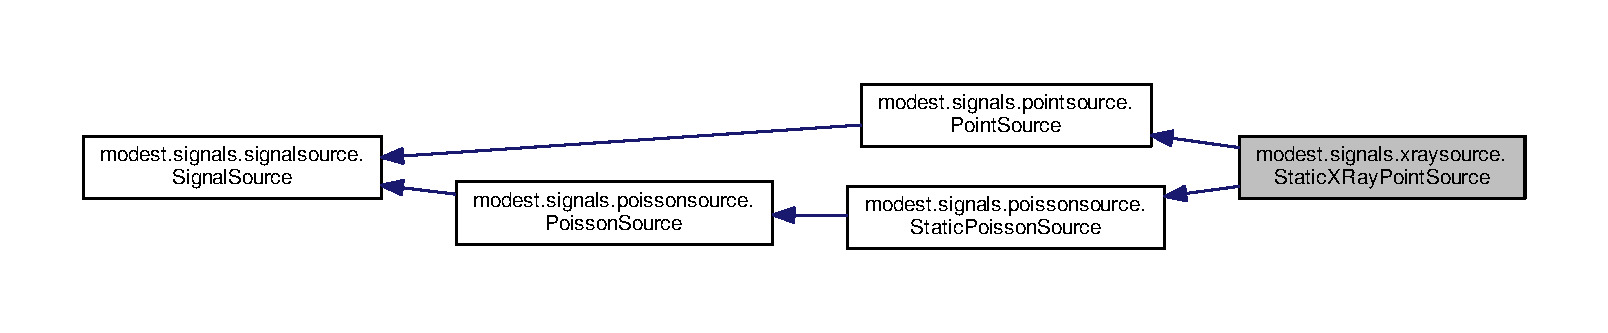
\includegraphics[width=350pt]{classmodest_1_1signals_1_1xraysource_1_1StaticXRayPointSource__inherit__graph}
\end{center}
\end{figure}


Collaboration diagram for modest.\+signals.\+xraysource.\+Static\+X\+Ray\+Point\+Source\+:\nopagebreak
\begin{figure}[H]
\begin{center}
\leavevmode
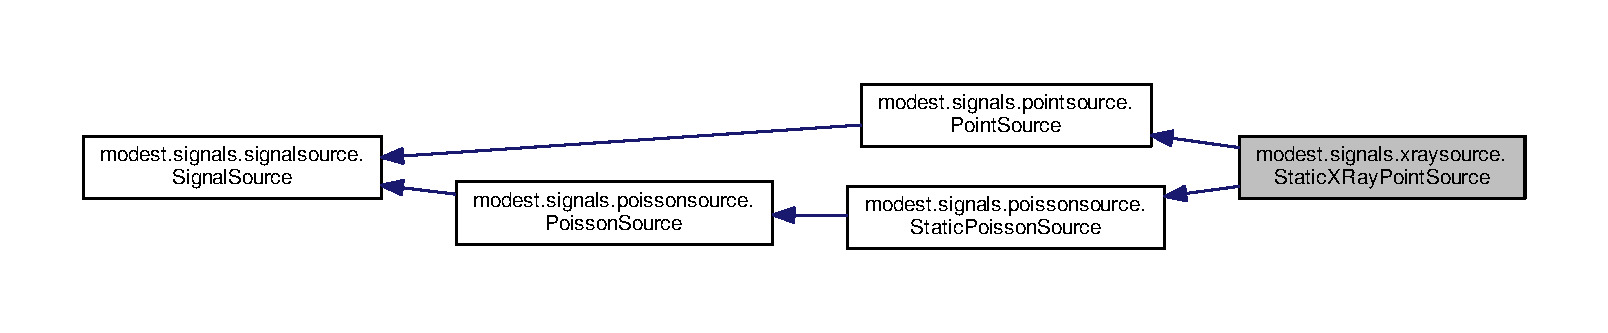
\includegraphics[width=350pt]{classmodest_1_1signals_1_1xraysource_1_1StaticXRayPointSource__coll__graph}
\end{center}
\end{figure}
\subsection*{Public Member Functions}
\begin{DoxyCompactItemize}
\item 
def \hyperlink{classmodest_1_1signals_1_1xraysource_1_1StaticXRayPointSource_abf7bfb177879d4c923da7fbd3d20070e}{\+\_\+\+\_\+init\+\_\+\+\_\+} (self, RA, D\+EC, \hyperlink{classmodest_1_1signals_1_1xraysource_1_1StaticXRayPointSource_a45c2430decc163480da7732af27d1f99}{peak\+Photon\+Flux}, \hyperlink{classmodest_1_1signals_1_1pointsource_1_1PointSource_a0924a2233bb4fd23e50d024e4f1b048e}{attitude\+State\+Name}=\textquotesingle{}attitude\textquotesingle{})
\item 
def \hyperlink{classmodest_1_1signals_1_1xraysource_1_1StaticXRayPointSource_acc2579a19ffce3dffd4dda4ddc66c265}{compute\+Association\+Probability} (self, measurement, state\+Dict, validation\+Threshold=0)
\item 
def \hyperlink{classmodest_1_1signals_1_1pointsource_1_1PointSource_a295eb1a487e18c77029585ac2785db80}{Ra\+Dec} (self)
\item 
def \hyperlink{classmodest_1_1signals_1_1pointsource_1_1PointSource_aa51308fcb654e7183d332ed824965397}{unit\+Vec} (self, \hyperlink{classmodest_1_1signals_1_1pointsource_1_1PointSource_a295eb1a487e18c77029585ac2785db80}{Ra\+Dec})
\item 
def \hyperlink{classmodest_1_1signals_1_1signalsource_1_1SignalSource_a9a64c6a9c2954f6ad61e4ca3518ea8ab}{signal\+ID} (self)
\item 
def \hyperlink{classmodest_1_1signals_1_1poissonsource_1_1StaticPoissonSource_a1754d94bff46d97817438bab552afef9}{compute\+Association\+Probability} (self, measurement)
\item 
def \hyperlink{classmodest_1_1signals_1_1poissonsource_1_1PoissonSource_a2f8a73e6f51cbdcd0f1e646d6f4d4574}{compute\+Association\+Probability} (self, current\+Flux, measurement)
\item 
def \hyperlink{classmodest_1_1signals_1_1signalsource_1_1SignalSource_a9a64c6a9c2954f6ad61e4ca3518ea8ab}{signal\+ID} (self)
\end{DoxyCompactItemize}
\subsection*{Public Attributes}
\begin{DoxyCompactItemize}
\item 
\hyperlink{classmodest_1_1signals_1_1xraysource_1_1StaticXRayPointSource_a45c2430decc163480da7732af27d1f99}{peak\+Photon\+Flux}
\item 
\hyperlink{classmodest_1_1signals_1_1pointsource_1_1PointSource_a0924a2233bb4fd23e50d024e4f1b048e}{attitude\+State\+Name}
\item 
\hyperlink{classmodest_1_1signals_1_1poissonsource_1_1PoissonSource_a34395fc83bd8743a0a5ee69f9392a606}{last\+Time}
\item 
\hyperlink{classmodest_1_1signals_1_1poissonsource_1_1PoissonSource_a6f2c657ad936b921715d826ac74f7fe5}{flux}
\end{DoxyCompactItemize}
\subsection*{Static Public Attributes}
\begin{DoxyCompactItemize}
\item 
int \hyperlink{classmodest_1_1signals_1_1signalsource_1_1SignalSource_a453eafb550b551adbec0903deb63dfce}{next\+Signal\+ID} = 0
\item 
int \hyperlink{classmodest_1_1signals_1_1signalsource_1_1SignalSource_a453eafb550b551adbec0903deb63dfce}{next\+Signal\+ID} = 0
\end{DoxyCompactItemize}


\subsection{Detailed Description}


Definition at line 15 of file xraysource.\+py.



\subsection{Constructor \& Destructor Documentation}
\index{modest\+::signals\+::xraysource\+::\+Static\+X\+Ray\+Point\+Source@{modest\+::signals\+::xraysource\+::\+Static\+X\+Ray\+Point\+Source}!\+\_\+\+\_\+init\+\_\+\+\_\+@{\+\_\+\+\_\+init\+\_\+\+\_\+}}
\index{\+\_\+\+\_\+init\+\_\+\+\_\+@{\+\_\+\+\_\+init\+\_\+\+\_\+}!modest\+::signals\+::xraysource\+::\+Static\+X\+Ray\+Point\+Source@{modest\+::signals\+::xraysource\+::\+Static\+X\+Ray\+Point\+Source}}
\subsubsection[{\texorpdfstring{\+\_\+\+\_\+init\+\_\+\+\_\+(self, R\+A, D\+E\+C, peak\+Photon\+Flux, attitude\+State\+Name=\textquotesingle{}attitude\textquotesingle{})}{__init__(self, RA, DEC, peakPhotonFlux, attitudeStateName='attitude')}}]{\setlength{\rightskip}{0pt plus 5cm}def modest.\+signals.\+xraysource.\+Static\+X\+Ray\+Point\+Source.\+\_\+\+\_\+init\+\_\+\+\_\+ (
\begin{DoxyParamCaption}
\item[{}]{self, }
\item[{}]{RA, }
\item[{}]{D\+EC, }
\item[{}]{peak\+Photon\+Flux, }
\item[{}]{attitude\+State\+Name = {\ttfamily \textquotesingle{}attitude\textquotesingle{}}}
\end{DoxyParamCaption}
)}\hypertarget{classmodest_1_1signals_1_1xraysource_1_1StaticXRayPointSource_abf7bfb177879d4c923da7fbd3d20070e}{}\label{classmodest_1_1signals_1_1xraysource_1_1StaticXRayPointSource_abf7bfb177879d4c923da7fbd3d20070e}


Definition at line 23 of file xraysource.\+py.



\subsection{Member Function Documentation}
\index{modest\+::signals\+::xraysource\+::\+Static\+X\+Ray\+Point\+Source@{modest\+::signals\+::xraysource\+::\+Static\+X\+Ray\+Point\+Source}!compute\+Association\+Probability@{compute\+Association\+Probability}}
\index{compute\+Association\+Probability@{compute\+Association\+Probability}!modest\+::signals\+::xraysource\+::\+Static\+X\+Ray\+Point\+Source@{modest\+::signals\+::xraysource\+::\+Static\+X\+Ray\+Point\+Source}}
\subsubsection[{\texorpdfstring{compute\+Association\+Probability(self, current\+Flux, measurement)}{computeAssociationProbability(self, currentFlux, measurement)}}]{\setlength{\rightskip}{0pt plus 5cm}def modest.\+signals.\+poissonsource.\+Poisson\+Source.\+compute\+Association\+Probability (
\begin{DoxyParamCaption}
\item[{}]{self, }
\item[{}]{current\+Flux, }
\item[{}]{measurement}
\end{DoxyParamCaption}
)\hspace{0.3cm}{\ttfamily [inherited]}}\hypertarget{classmodest_1_1signals_1_1poissonsource_1_1PoissonSource_a2f8a73e6f51cbdcd0f1e646d6f4d4574}{}\label{classmodest_1_1signals_1_1poissonsource_1_1PoissonSource_a2f8a73e6f51cbdcd0f1e646d6f4d4574}


Definition at line 21 of file poissonsource.\+py.

\index{modest\+::signals\+::xraysource\+::\+Static\+X\+Ray\+Point\+Source@{modest\+::signals\+::xraysource\+::\+Static\+X\+Ray\+Point\+Source}!compute\+Association\+Probability@{compute\+Association\+Probability}}
\index{compute\+Association\+Probability@{compute\+Association\+Probability}!modest\+::signals\+::xraysource\+::\+Static\+X\+Ray\+Point\+Source@{modest\+::signals\+::xraysource\+::\+Static\+X\+Ray\+Point\+Source}}
\subsubsection[{\texorpdfstring{compute\+Association\+Probability(self, measurement, state\+Dict, validation\+Threshold=0)}{computeAssociationProbability(self, measurement, stateDict, validationThreshold=0)}}]{\setlength{\rightskip}{0pt plus 5cm}def modest.\+signals.\+xraysource.\+Static\+X\+Ray\+Point\+Source.\+compute\+Association\+Probability (
\begin{DoxyParamCaption}
\item[{}]{self, }
\item[{}]{measurement, }
\item[{}]{state\+Dict, }
\item[{}]{validation\+Threshold = {\ttfamily 0}}
\end{DoxyParamCaption}
)}\hypertarget{classmodest_1_1signals_1_1xraysource_1_1StaticXRayPointSource_acc2579a19ffce3dffd4dda4ddc66c265}{}\label{classmodest_1_1signals_1_1xraysource_1_1StaticXRayPointSource_acc2579a19ffce3dffd4dda4ddc66c265}


Definition at line 36 of file xraysource.\+py.

\index{modest\+::signals\+::xraysource\+::\+Static\+X\+Ray\+Point\+Source@{modest\+::signals\+::xraysource\+::\+Static\+X\+Ray\+Point\+Source}!compute\+Association\+Probability@{compute\+Association\+Probability}}
\index{compute\+Association\+Probability@{compute\+Association\+Probability}!modest\+::signals\+::xraysource\+::\+Static\+X\+Ray\+Point\+Source@{modest\+::signals\+::xraysource\+::\+Static\+X\+Ray\+Point\+Source}}
\subsubsection[{\texorpdfstring{compute\+Association\+Probability(self, measurement)}{computeAssociationProbability(self, measurement)}}]{\setlength{\rightskip}{0pt plus 5cm}def modest.\+signals.\+poissonsource.\+Static\+Poisson\+Source.\+compute\+Association\+Probability (
\begin{DoxyParamCaption}
\item[{}]{self, }
\item[{}]{measurement}
\end{DoxyParamCaption}
)\hspace{0.3cm}{\ttfamily [inherited]}}\hypertarget{classmodest_1_1signals_1_1poissonsource_1_1StaticPoissonSource_a1754d94bff46d97817438bab552afef9}{}\label{classmodest_1_1signals_1_1poissonsource_1_1StaticPoissonSource_a1754d94bff46d97817438bab552afef9}


Definition at line 38 of file poissonsource.\+py.

\index{modest\+::signals\+::xraysource\+::\+Static\+X\+Ray\+Point\+Source@{modest\+::signals\+::xraysource\+::\+Static\+X\+Ray\+Point\+Source}!Ra\+Dec@{Ra\+Dec}}
\index{Ra\+Dec@{Ra\+Dec}!modest\+::signals\+::xraysource\+::\+Static\+X\+Ray\+Point\+Source@{modest\+::signals\+::xraysource\+::\+Static\+X\+Ray\+Point\+Source}}
\subsubsection[{\texorpdfstring{Ra\+Dec(self)}{RaDec(self)}}]{\setlength{\rightskip}{0pt plus 5cm}def modest.\+signals.\+pointsource.\+Point\+Source.\+Ra\+Dec (
\begin{DoxyParamCaption}
\item[{}]{self}
\end{DoxyParamCaption}
)\hspace{0.3cm}{\ttfamily [inherited]}}\hypertarget{classmodest_1_1signals_1_1pointsource_1_1PointSource_a295eb1a487e18c77029585ac2785db80}{}\label{classmodest_1_1signals_1_1pointsource_1_1PointSource_a295eb1a487e18c77029585ac2785db80}


Definition at line 21 of file pointsource.\+py.

\index{modest\+::signals\+::xraysource\+::\+Static\+X\+Ray\+Point\+Source@{modest\+::signals\+::xraysource\+::\+Static\+X\+Ray\+Point\+Source}!signal\+ID@{signal\+ID}}
\index{signal\+ID@{signal\+ID}!modest\+::signals\+::xraysource\+::\+Static\+X\+Ray\+Point\+Source@{modest\+::signals\+::xraysource\+::\+Static\+X\+Ray\+Point\+Source}}
\subsubsection[{\texorpdfstring{signal\+I\+D(self)}{signalID(self)}}]{\setlength{\rightskip}{0pt plus 5cm}def modest.\+signals.\+signalsource.\+Signal\+Source.\+signal\+ID (
\begin{DoxyParamCaption}
\item[{}]{self}
\end{DoxyParamCaption}
)\hspace{0.3cm}{\ttfamily [inherited]}}\hypertarget{classmodest_1_1signals_1_1signalsource_1_1SignalSource_a9a64c6a9c2954f6ad61e4ca3518ea8ab}{}\label{classmodest_1_1signals_1_1signalsource_1_1SignalSource_a9a64c6a9c2954f6ad61e4ca3518ea8ab}


Definition at line 17 of file signalsource.\+py.

\index{modest\+::signals\+::xraysource\+::\+Static\+X\+Ray\+Point\+Source@{modest\+::signals\+::xraysource\+::\+Static\+X\+Ray\+Point\+Source}!signal\+ID@{signal\+ID}}
\index{signal\+ID@{signal\+ID}!modest\+::signals\+::xraysource\+::\+Static\+X\+Ray\+Point\+Source@{modest\+::signals\+::xraysource\+::\+Static\+X\+Ray\+Point\+Source}}
\subsubsection[{\texorpdfstring{signal\+I\+D(self)}{signalID(self)}}]{\setlength{\rightskip}{0pt plus 5cm}def modest.\+signals.\+signalsource.\+Signal\+Source.\+signal\+ID (
\begin{DoxyParamCaption}
\item[{}]{self}
\end{DoxyParamCaption}
)\hspace{0.3cm}{\ttfamily [inherited]}}\hypertarget{classmodest_1_1signals_1_1signalsource_1_1SignalSource_a9a64c6a9c2954f6ad61e4ca3518ea8ab}{}\label{classmodest_1_1signals_1_1signalsource_1_1SignalSource_a9a64c6a9c2954f6ad61e4ca3518ea8ab}


Definition at line 17 of file signalsource.\+py.

\index{modest\+::signals\+::xraysource\+::\+Static\+X\+Ray\+Point\+Source@{modest\+::signals\+::xraysource\+::\+Static\+X\+Ray\+Point\+Source}!unit\+Vec@{unit\+Vec}}
\index{unit\+Vec@{unit\+Vec}!modest\+::signals\+::xraysource\+::\+Static\+X\+Ray\+Point\+Source@{modest\+::signals\+::xraysource\+::\+Static\+X\+Ray\+Point\+Source}}
\subsubsection[{\texorpdfstring{unit\+Vec(self, Ra\+Dec)}{unitVec(self, RaDec)}}]{\setlength{\rightskip}{0pt plus 5cm}def modest.\+signals.\+pointsource.\+Point\+Source.\+unit\+Vec (
\begin{DoxyParamCaption}
\item[{}]{self, }
\item[{}]{Ra\+Dec}
\end{DoxyParamCaption}
)\hspace{0.3cm}{\ttfamily [inherited]}}\hypertarget{classmodest_1_1signals_1_1pointsource_1_1PointSource_aa51308fcb654e7183d332ed824965397}{}\label{classmodest_1_1signals_1_1pointsource_1_1PointSource_aa51308fcb654e7183d332ed824965397}


Definition at line 26 of file pointsource.\+py.



\subsection{Member Data Documentation}
\index{modest\+::signals\+::xraysource\+::\+Static\+X\+Ray\+Point\+Source@{modest\+::signals\+::xraysource\+::\+Static\+X\+Ray\+Point\+Source}!attitude\+State\+Name@{attitude\+State\+Name}}
\index{attitude\+State\+Name@{attitude\+State\+Name}!modest\+::signals\+::xraysource\+::\+Static\+X\+Ray\+Point\+Source@{modest\+::signals\+::xraysource\+::\+Static\+X\+Ray\+Point\+Source}}
\subsubsection[{\texorpdfstring{attitude\+State\+Name}{attitudeStateName}}]{\setlength{\rightskip}{0pt plus 5cm}modest.\+signals.\+pointsource.\+Point\+Source.\+attitude\+State\+Name\hspace{0.3cm}{\ttfamily [inherited]}}\hypertarget{classmodest_1_1signals_1_1pointsource_1_1PointSource_a0924a2233bb4fd23e50d024e4f1b048e}{}\label{classmodest_1_1signals_1_1pointsource_1_1PointSource_a0924a2233bb4fd23e50d024e4f1b048e}


Definition at line 17 of file pointsource.\+py.

\index{modest\+::signals\+::xraysource\+::\+Static\+X\+Ray\+Point\+Source@{modest\+::signals\+::xraysource\+::\+Static\+X\+Ray\+Point\+Source}!flux@{flux}}
\index{flux@{flux}!modest\+::signals\+::xraysource\+::\+Static\+X\+Ray\+Point\+Source@{modest\+::signals\+::xraysource\+::\+Static\+X\+Ray\+Point\+Source}}
\subsubsection[{\texorpdfstring{flux}{flux}}]{\setlength{\rightskip}{0pt plus 5cm}modest.\+signals.\+poissonsource.\+Poisson\+Source.\+flux\hspace{0.3cm}{\ttfamily [inherited]}}\hypertarget{classmodest_1_1signals_1_1poissonsource_1_1PoissonSource_a6f2c657ad936b921715d826ac74f7fe5}{}\label{classmodest_1_1signals_1_1poissonsource_1_1PoissonSource_a6f2c657ad936b921715d826ac74f7fe5}


Definition at line 14 of file poissonsource.\+py.

\index{modest\+::signals\+::xraysource\+::\+Static\+X\+Ray\+Point\+Source@{modest\+::signals\+::xraysource\+::\+Static\+X\+Ray\+Point\+Source}!last\+Time@{last\+Time}}
\index{last\+Time@{last\+Time}!modest\+::signals\+::xraysource\+::\+Static\+X\+Ray\+Point\+Source@{modest\+::signals\+::xraysource\+::\+Static\+X\+Ray\+Point\+Source}}
\subsubsection[{\texorpdfstring{last\+Time}{lastTime}}]{\setlength{\rightskip}{0pt plus 5cm}modest.\+signals.\+poissonsource.\+Poisson\+Source.\+last\+Time\hspace{0.3cm}{\ttfamily [inherited]}}\hypertarget{classmodest_1_1signals_1_1poissonsource_1_1PoissonSource_a34395fc83bd8743a0a5ee69f9392a606}{}\label{classmodest_1_1signals_1_1poissonsource_1_1PoissonSource_a34395fc83bd8743a0a5ee69f9392a606}


Definition at line 13 of file poissonsource.\+py.

\index{modest\+::signals\+::xraysource\+::\+Static\+X\+Ray\+Point\+Source@{modest\+::signals\+::xraysource\+::\+Static\+X\+Ray\+Point\+Source}!next\+Signal\+ID@{next\+Signal\+ID}}
\index{next\+Signal\+ID@{next\+Signal\+ID}!modest\+::signals\+::xraysource\+::\+Static\+X\+Ray\+Point\+Source@{modest\+::signals\+::xraysource\+::\+Static\+X\+Ray\+Point\+Source}}
\subsubsection[{\texorpdfstring{next\+Signal\+ID}{nextSignalID}}]{\setlength{\rightskip}{0pt plus 5cm}int modest.\+signals.\+signalsource.\+Signal\+Source.\+next\+Signal\+ID = 0\hspace{0.3cm}{\ttfamily [static]}, {\ttfamily [inherited]}}\hypertarget{classmodest_1_1signals_1_1signalsource_1_1SignalSource_a453eafb550b551adbec0903deb63dfce}{}\label{classmodest_1_1signals_1_1signalsource_1_1SignalSource_a453eafb550b551adbec0903deb63dfce}


Definition at line 8 of file signalsource.\+py.

\index{modest\+::signals\+::xraysource\+::\+Static\+X\+Ray\+Point\+Source@{modest\+::signals\+::xraysource\+::\+Static\+X\+Ray\+Point\+Source}!next\+Signal\+ID@{next\+Signal\+ID}}
\index{next\+Signal\+ID@{next\+Signal\+ID}!modest\+::signals\+::xraysource\+::\+Static\+X\+Ray\+Point\+Source@{modest\+::signals\+::xraysource\+::\+Static\+X\+Ray\+Point\+Source}}
\subsubsection[{\texorpdfstring{next\+Signal\+ID}{nextSignalID}}]{\setlength{\rightskip}{0pt plus 5cm}int modest.\+signals.\+signalsource.\+Signal\+Source.\+next\+Signal\+ID = 0\hspace{0.3cm}{\ttfamily [static]}, {\ttfamily [inherited]}}\hypertarget{classmodest_1_1signals_1_1signalsource_1_1SignalSource_a453eafb550b551adbec0903deb63dfce}{}\label{classmodest_1_1signals_1_1signalsource_1_1SignalSource_a453eafb550b551adbec0903deb63dfce}


Definition at line 8 of file signalsource.\+py.

\index{modest\+::signals\+::xraysource\+::\+Static\+X\+Ray\+Point\+Source@{modest\+::signals\+::xraysource\+::\+Static\+X\+Ray\+Point\+Source}!peak\+Photon\+Flux@{peak\+Photon\+Flux}}
\index{peak\+Photon\+Flux@{peak\+Photon\+Flux}!modest\+::signals\+::xraysource\+::\+Static\+X\+Ray\+Point\+Source@{modest\+::signals\+::xraysource\+::\+Static\+X\+Ray\+Point\+Source}}
\subsubsection[{\texorpdfstring{peak\+Photon\+Flux}{peakPhotonFlux}}]{\setlength{\rightskip}{0pt plus 5cm}modest.\+signals.\+xraysource.\+Static\+X\+Ray\+Point\+Source.\+peak\+Photon\+Flux}\hypertarget{classmodest_1_1signals_1_1xraysource_1_1StaticXRayPointSource_a45c2430decc163480da7732af27d1f99}{}\label{classmodest_1_1signals_1_1xraysource_1_1StaticXRayPointSource_a45c2430decc163480da7732af27d1f99}


Definition at line 27 of file xraysource.\+py.



The documentation for this class was generated from the following file\+:\begin{DoxyCompactItemize}
\item 
modest/signals/\hyperlink{xraysource_8py}{xraysource.\+py}\end{DoxyCompactItemize}

\hypertarget{classmodest_1_1substates_1_1substate_1_1SubState}{}\section{modest.\+substates.\+substate.\+Sub\+State Class Reference}
\label{classmodest_1_1substates_1_1substate_1_1SubState}\index{modest.\+substates.\+substate.\+Sub\+State@{modest.\+substates.\+substate.\+Sub\+State}}


This is an abstract base class for objects used as sub-\/states in State.\+Modular\+Filter.  




Inheritance diagram for modest.\+substates.\+substate.\+Sub\+State\+:\nopagebreak
\begin{figure}[H]
\begin{center}
\leavevmode
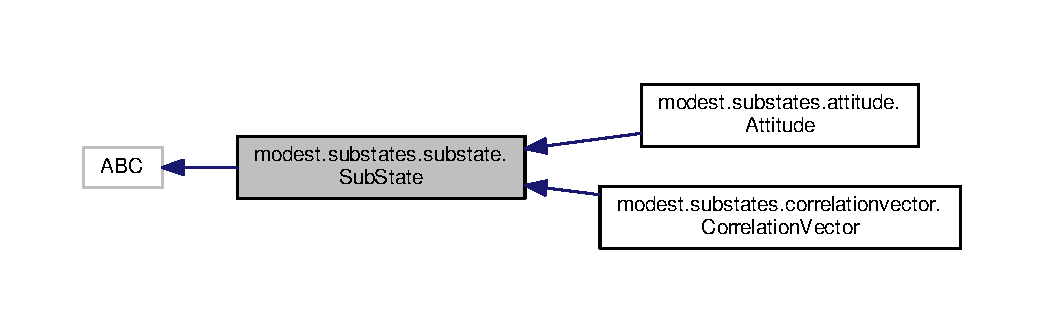
\includegraphics[width=350pt]{classmodest_1_1substates_1_1substate_1_1SubState__inherit__graph}
\end{center}
\end{figure}


Collaboration diagram for modest.\+substates.\+substate.\+Sub\+State\+:\nopagebreak
\begin{figure}[H]
\begin{center}
\leavevmode
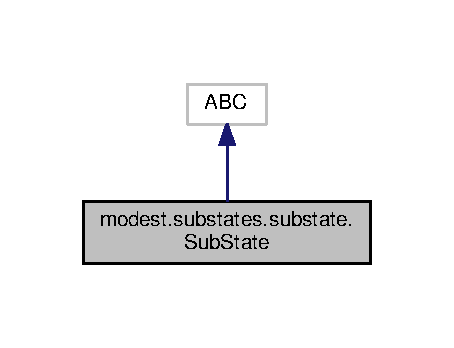
\includegraphics[width=218pt]{classmodest_1_1substates_1_1substate_1_1SubState__coll__graph}
\end{center}
\end{figure}
\subsection*{Public Member Functions}
\begin{DoxyCompactItemize}
\item 
def \hyperlink{classmodest_1_1substates_1_1substate_1_1SubState_a51fb99c0857f81ea659ffeca810672a3}{\+\_\+\+\_\+init\+\_\+\+\_\+} (self, state\+Dimension=None, \hyperlink{classmodest_1_1substates_1_1substate_1_1SubState_a38c12c9d0899bc1161f3502b584517a2}{state\+Vector\+History}=None)
\begin{DoxyCompactList}\small\item\em \hyperlink{classmodest_1_1substates_1_1substate_1_1SubState_a51fb99c0857f81ea659ffeca810672a3}{\+\_\+\+\_\+init\+\_\+\+\_\+} initializes a \hyperlink{classmodest_1_1substates_1_1substate_1_1SubState}{Sub\+State} object \end{DoxyCompactList}\end{DoxyCompactItemize}
\begin{Indent}{\bf Mandatory Sub\+State Functions}\par
{\em The following functions are functions which are required for the \hyperlink{classmodest_1_1substates_1_1substate_1_1SubState}{Sub\+State} to function as a sub-\/state in State.\+Modular\+Filter. }\begin{DoxyCompactItemize}
\item 
def \hyperlink{classmodest_1_1substates_1_1substate_1_1SubState_aa18c8238415131b4b63cef0e4b2ff9fd}{get\+State\+Vector} (self)
\begin{DoxyCompactList}\small\item\em \hyperlink{classmodest_1_1substates_1_1substate_1_1SubState_aa18c8238415131b4b63cef0e4b2ff9fd}{get\+State\+Vector} returns the most recent value of the state vector \end{DoxyCompactList}\item 
def \hyperlink{classmodest_1_1substates_1_1substate_1_1SubState_a3644149dc4cc19c0e32d0b7040998c96}{store\+State\+Vector} (self, sv\+Dict)
\begin{DoxyCompactList}\small\item\em \hyperlink{classmodest_1_1substates_1_1substate_1_1SubState_a3644149dc4cc19c0e32d0b7040998c96}{store\+State\+Vector} stores the most recent value of the state vector. \end{DoxyCompactList}\item 
def \hyperlink{classmodest_1_1substates_1_1substate_1_1SubState_a6e308aadd13962e476d2892ec728e3a5}{covariance} (self)
\begin{DoxyCompactList}\small\item\em \hyperlink{classmodest_1_1substates_1_1substate_1_1SubState_a6e308aadd13962e476d2892ec728e3a5}{covariance} returns the \hyperlink{classmodest_1_1substates_1_1substate_1_1SubState}{Sub\+State} covariance matrix \end{DoxyCompactList}\item 
def \hyperlink{classmodest_1_1substates_1_1substate_1_1SubState_ab9027f6d1d7d57c47731612f519b7ee6}{dimension} (self)
\begin{DoxyCompactList}\small\item\em \hyperlink{classmodest_1_1substates_1_1substate_1_1SubState_ab9027f6d1d7d57c47731612f519b7ee6}{dimension} returns the dimension of the sub-\/state vector \end{DoxyCompactList}\item 
def \hyperlink{classmodest_1_1substates_1_1substate_1_1SubState_a06d147fa5babe4e147b3267e67054ab4}{time\+Update} (self, dT, dynamics=None)
\begin{DoxyCompactList}\small\item\em \hyperlink{classmodest_1_1substates_1_1substate_1_1SubState_a06d147fa5babe4e147b3267e67054ab4}{time\+Update} returns time-\/update matrices \end{DoxyCompactList}\item 
def \hyperlink{classmodest_1_1substates_1_1substate_1_1SubState_a98901b80c96264945362ec50b489a636}{get\+Measurement\+Matrices} (self, measurement, source=None)
\begin{DoxyCompactList}\small\item\em \hyperlink{classmodest_1_1substates_1_1substate_1_1SubState_aa18c8238415131b4b63cef0e4b2ff9fd}{get\+State\+Vector} returns the most recent value of the state vector \end{DoxyCompactList}\end{DoxyCompactItemize}
\end{Indent}
\begin{Indent}{\bf Plotting Functions}\par
{\em These functions provide generalized plotting capabilities }\begin{DoxyCompactItemize}
\item 
def \hyperlink{classmodest_1_1substates_1_1substate_1_1SubState_a1adac64be88eab0a64bb952518c4268f}{initialize\+Real\+Time\+Plot} (self, plot\+Handle=None, axis\+Handle=None)
\item 
def \hyperlink{classmodest_1_1substates_1_1substate_1_1SubState_a2deb7d1ca3105eb20e50fa7e67298355}{real\+Time\+Plot} (self, normalized=True)
\end{DoxyCompactItemize}
\end{Indent}
\subsection*{Public Attributes}
\begin{DoxyCompactItemize}
\item 
\hyperlink{classmodest_1_1substates_1_1substate_1_1SubState_a38c12c9d0899bc1161f3502b584517a2}{state\+Vector\+History}
\begin{DoxyCompactList}\small\item\em Stores the time-\/history of the sub-\/state state vector. \end{DoxyCompactList}\item 
\hyperlink{classmodest_1_1substates_1_1substate_1_1SubState_a37ded775b84cea85b4dce0f1b16286c4}{R\+T\+Plot\+Handle}
\begin{DoxyCompactList}\small\item\em Stores handle for real-\/time plotting. \end{DoxyCompactList}\item 
\hyperlink{classmodest_1_1substates_1_1substate_1_1SubState_a9fefae1facc797a1132fb61a55e9ffa1}{R\+T\+Plot\+Data}
\item 
\hyperlink{classmodest_1_1substates_1_1substate_1_1SubState_a497ccbb6658589b02568e87c6382222e}{R\+T\+Paxis\+Handle}
\end{DoxyCompactItemize}
\subsection*{Private Attributes}
\begin{DoxyCompactItemize}
\item 
\hyperlink{classmodest_1_1substates_1_1substate_1_1SubState_a5b1c0756a69da7f293a415c7d2d77843}{\+\_\+\+\_\+dimension\+\_\+\+\_\+}
\begin{DoxyCompactList}\small\item\em Stores the length of the state vector as seen by the \hyperlink{namespacemodest_1_1ModularFilter}{Modular\+Filter}. \end{DoxyCompactList}\end{DoxyCompactItemize}


\subsection{Detailed Description}
This is an abstract base class for objects used as sub-\/states in State.\+Modular\+Filter. 

\hyperlink{classmodest_1_1substates_1_1substate_1_1SubState}{Sub\+State} is an abstract base class that specifies the methods which are required for an object to function as a sub-\/state of State.\+Modular\+Filter.

Some of these methods are implemented and most likely do not need to be reimplemented in a derived class implementation (for example the \hyperlink{classmodest_1_1substates_1_1substate_1_1SubState_ab9027f6d1d7d57c47731612f519b7ee6}{dimension} and \hyperlink{classmodest_1_1substates_1_1substate_1_1SubState_a6e308aadd13962e476d2892ec728e3a5}{covariance} methods.

Other methods may have a rudimentary implementation that may be suitable for some derived classes, but not others, depending on the specific functionality of the derived class (for instance \hyperlink{classmodest_1_1substates_1_1substate_1_1SubState_aa18c8238415131b4b63cef0e4b2ff9fd}{get\+State\+Vector} and \hyperlink{classmodest_1_1substates_1_1substate_1_1SubState_a3644149dc4cc19c0e32d0b7040998c96}{store\+State\+Vector}).

Finally, some methods are specifically tagged as abstract methods and are not implemented at all. These methods must be implemented in the derived class. This is usually because there is no way to implement even a rudimentary version of what the method is supposed to do without having some knowledge of what kind of substate the derived class contains (for instance \hyperlink{classmodest_1_1substates_1_1substate_1_1SubState_a06d147fa5babe4e147b3267e67054ab4}{time\+Update} and \hyperlink{classmodest_1_1substates_1_1substate_1_1SubState_a98901b80c96264945362ec50b489a636}{get\+Measurement\+Matrices}).

In any case, the documentation for each method of \hyperlink{classmodest_1_1substates_1_1substate_1_1SubState}{Sub\+State} contains a generalized description of what functionality the implementation should provide in a derived class. 

Definition at line 42 of file substate.\+py.



\subsection{Constructor \& Destructor Documentation}
\index{modest\+::substates\+::substate\+::\+Sub\+State@{modest\+::substates\+::substate\+::\+Sub\+State}!\+\_\+\+\_\+init\+\_\+\+\_\+@{\+\_\+\+\_\+init\+\_\+\+\_\+}}
\index{\+\_\+\+\_\+init\+\_\+\+\_\+@{\+\_\+\+\_\+init\+\_\+\+\_\+}!modest\+::substates\+::substate\+::\+Sub\+State@{modest\+::substates\+::substate\+::\+Sub\+State}}
\subsubsection[{\texorpdfstring{\+\_\+\+\_\+init\+\_\+\+\_\+(self, state\+Dimension=\+None, state\+Vector\+History=\+None)}{__init__(self, stateDimension=None, stateVectorHistory=None)}}]{\setlength{\rightskip}{0pt plus 5cm}def modest.\+substates.\+substate.\+Sub\+State.\+\_\+\+\_\+init\+\_\+\+\_\+ (
\begin{DoxyParamCaption}
\item[{}]{self, }
\item[{}]{state\+Dimension = {\ttfamily None}, }
\item[{}]{state\+Vector\+History = {\ttfamily None}}
\end{DoxyParamCaption}
)}\hypertarget{classmodest_1_1substates_1_1substate_1_1SubState_a51fb99c0857f81ea659ffeca810672a3}{}\label{classmodest_1_1substates_1_1substate_1_1SubState_a51fb99c0857f81ea659ffeca810672a3}


\hyperlink{classmodest_1_1substates_1_1substate_1_1SubState_a51fb99c0857f81ea659ffeca810672a3}{\+\_\+\+\_\+init\+\_\+\+\_\+} initializes a \hyperlink{classmodest_1_1substates_1_1substate_1_1SubState}{Sub\+State} object 

The \hyperlink{classmodest_1_1substates_1_1substate_1_1SubState_a51fb99c0857f81ea659ffeca810672a3}{\+\_\+\+\_\+init\+\_\+\+\_\+} method is responsible for initializing a generalized \hyperlink{classmodest_1_1substates_1_1substate_1_1SubState}{Sub\+State} object. The essential functions of \hyperlink{classmodest_1_1substates_1_1substate_1_1SubState_a51fb99c0857f81ea659ffeca810672a3}{\+\_\+\+\_\+init\+\_\+\+\_\+} are to store the dimension of the state, and to initialize a time-\/history of the state in a Smart\+Panda object.

If no values are passed for the initial state estimate dictionary, they will be initialized to the following default values.


\begin{DoxyItemize}
\item \textquotesingle{}state\+Vector\textquotesingle{}\+: A length \hyperlink{classmodest_1_1substates_1_1substate_1_1SubState_ab9027f6d1d7d57c47731612f519b7ee6}{dimension} array of zeros
\item \textquotesingle{}covariance\textquotesingle{}\+: An (\hyperlink{classmodest_1_1substates_1_1substate_1_1SubState_ab9027f6d1d7d57c47731612f519b7ee6}{dimension} x \hyperlink{classmodest_1_1substates_1_1substate_1_1SubState_ab9027f6d1d7d57c47731612f519b7ee6}{dimension}) identity matrix
\item \textquotesingle{}t\textquotesingle{}\+: 0
\end{DoxyItemize}


\begin{DoxyParams}{Parameters}
{\em self} & The object pointer \\
\hline
{\em state\+Dimension} & The dimension of the sub-\/state state vector \\
\hline
{\em state\+Vector\+History} & A dictionary containing the initial state. \\
\hline
\end{DoxyParams}


Definition at line 65 of file substate.\+py.



\subsection{Member Function Documentation}
\index{modest\+::substates\+::substate\+::\+Sub\+State@{modest\+::substates\+::substate\+::\+Sub\+State}!covariance@{covariance}}
\index{covariance@{covariance}!modest\+::substates\+::substate\+::\+Sub\+State@{modest\+::substates\+::substate\+::\+Sub\+State}}
\subsubsection[{\texorpdfstring{covariance(self)}{covariance(self)}}]{\setlength{\rightskip}{0pt plus 5cm}def modest.\+substates.\+substate.\+Sub\+State.\+covariance (
\begin{DoxyParamCaption}
\item[{}]{self}
\end{DoxyParamCaption}
)}\hypertarget{classmodest_1_1substates_1_1substate_1_1SubState_a6e308aadd13962e476d2892ec728e3a5}{}\label{classmodest_1_1substates_1_1substate_1_1SubState_a6e308aadd13962e476d2892ec728e3a5}


\hyperlink{classmodest_1_1substates_1_1substate_1_1SubState_a6e308aadd13962e476d2892ec728e3a5}{covariance} returns the \hyperlink{classmodest_1_1substates_1_1substate_1_1SubState}{Sub\+State} covariance matrix 

The \hyperlink{classmodest_1_1substates_1_1substate_1_1SubState_a6e308aadd13962e476d2892ec728e3a5}{covariance} method returns the covariance of the estimate of the substate.

\begin{DoxyRefDesc}{Todo}
\item[\hyperlink{todo__todo000001}{Todo}]Currently, this method only returns the covariance of the most recent state estimate. Ideally, there should be an optional time parameter which would allow the user to get the covaraince matrix at a specified time (or the closest to that specified time).\end{DoxyRefDesc}



\begin{DoxyParams}{Parameters}
{\em self} & The object pointer\\
\hline
\end{DoxyParams}
\begin{DoxyReturn}{Returns}
Returns the covaraince matrix 
\end{DoxyReturn}


Definition at line 172 of file substate.\+py.

\index{modest\+::substates\+::substate\+::\+Sub\+State@{modest\+::substates\+::substate\+::\+Sub\+State}!dimension@{dimension}}
\index{dimension@{dimension}!modest\+::substates\+::substate\+::\+Sub\+State@{modest\+::substates\+::substate\+::\+Sub\+State}}
\subsubsection[{\texorpdfstring{dimension(self)}{dimension(self)}}]{\setlength{\rightskip}{0pt plus 5cm}def modest.\+substates.\+substate.\+Sub\+State.\+dimension (
\begin{DoxyParamCaption}
\item[{}]{self}
\end{DoxyParamCaption}
)}\hypertarget{classmodest_1_1substates_1_1substate_1_1SubState_ab9027f6d1d7d57c47731612f519b7ee6}{}\label{classmodest_1_1substates_1_1substate_1_1SubState_ab9027f6d1d7d57c47731612f519b7ee6}


\hyperlink{classmodest_1_1substates_1_1substate_1_1SubState_ab9027f6d1d7d57c47731612f519b7ee6}{dimension} returns the dimension of the sub-\/state vector 

The \hyperlink{classmodest_1_1substates_1_1substate_1_1SubState_ab9027f6d1d7d57c47731612f519b7ee6}{dimension} method returns the dimension of the sub-\/state vector estimated by the \hyperlink{classmodest_1_1substates_1_1substate_1_1SubState}{Sub\+State}. This is the dimension as seen by the \hyperlink{namespacemodest_1_1ModularFilter}{Modular\+Filter} estimator.

The default implementation is to return the class variable \hyperlink{classmodest_1_1substates_1_1substate_1_1SubState_a5b1c0756a69da7f293a415c7d2d77843}{\+\_\+\+\_\+dimension\+\_\+\+\_\+}, which is saved at initialization. This is designated as a \char`\"{}protected\char`\"{} variable, and should not change during the course of the \hyperlink{classmodest_1_1substates_1_1substate_1_1SubState}{Sub\+State}\textquotesingle{}s lifetime. If child class overwrites this implementation, care should be taken to ensure that the value returned by \hyperlink{classmodest_1_1substates_1_1substate_1_1SubState_ab9027f6d1d7d57c47731612f519b7ee6}{dimension} does not change over \hyperlink{classmodest_1_1substates_1_1substate_1_1SubState}{Sub\+State} object lifetime.

For \hyperlink{classmodest_1_1substates_1_1substate_1_1SubState}{Sub\+State} objects with auxilary states, or other quantities related to the state vector but not directly estimated by the \hyperlink{namespacemodest_1_1ModularFilter}{Modular\+Filter}, \hyperlink{classmodest_1_1substates_1_1substate_1_1SubState_ab9027f6d1d7d57c47731612f519b7ee6}{dimension} should not count these states as part of the total dimension.


\begin{DoxyParams}{Parameters}
{\em self} & The object pointer\\
\hline
\end{DoxyParams}
\begin{DoxyReturn}{Returns}
Returns the dimension of state vector 
\end{DoxyReturn}


Definition at line 197 of file substate.\+py.

\index{modest\+::substates\+::substate\+::\+Sub\+State@{modest\+::substates\+::substate\+::\+Sub\+State}!get\+Measurement\+Matrices@{get\+Measurement\+Matrices}}
\index{get\+Measurement\+Matrices@{get\+Measurement\+Matrices}!modest\+::substates\+::substate\+::\+Sub\+State@{modest\+::substates\+::substate\+::\+Sub\+State}}
\subsubsection[{\texorpdfstring{get\+Measurement\+Matrices(self, measurement, source=\+None)}{getMeasurementMatrices(self, measurement, source=None)}}]{\setlength{\rightskip}{0pt plus 5cm}def modest.\+substates.\+substate.\+Sub\+State.\+get\+Measurement\+Matrices (
\begin{DoxyParamCaption}
\item[{}]{self, }
\item[{}]{measurement, }
\item[{}]{source = {\ttfamily None}}
\end{DoxyParamCaption}
)}\hypertarget{classmodest_1_1substates_1_1substate_1_1SubState_a98901b80c96264945362ec50b489a636}{}\label{classmodest_1_1substates_1_1substate_1_1SubState_a98901b80c96264945362ec50b489a636}


\hyperlink{classmodest_1_1substates_1_1substate_1_1SubState_aa18c8238415131b4b63cef0e4b2ff9fd}{get\+State\+Vector} returns the most recent value of the state vector 

The \hyperlink{classmodest_1_1substates_1_1substate_1_1SubState_aa18c8238415131b4b63cef0e4b2ff9fd}{get\+State\+Vector} method is responsible for returning a dictionary object containing, at minimim, the following items\+:


\begin{DoxyItemize}
\item \textquotesingle{}state\+Vector\textquotesingle{}\+: A length \hyperlink{classmodest_1_1substates_1_1substate_1_1SubState_ab9027f6d1d7d57c47731612f519b7ee6}{dimension} array containing the most recent state vector estimate
\item \textquotesingle{}covariance\textquotesingle{}\+: A (\hyperlink{classmodest_1_1substates_1_1substate_1_1SubState_ab9027f6d1d7d57c47731612f519b7ee6}{dimension} x \hyperlink{classmodest_1_1substates_1_1substate_1_1SubState_ab9027f6d1d7d57c47731612f519b7ee6}{dimension}) array containing the most recent covariance matrix
\item \textquotesingle{}a\+Priori\textquotesingle{}\+: A boolean indicating if the most recent estimate is the
\item result of a time update (a\+Priori=True) or a measurement update (a\+Priori=False)
\end{DoxyItemize}

This function can be used as-\/is


\begin{DoxyParams}{Parameters}
{\em self} & The object pointer\\
\hline
\end{DoxyParams}
\begin{DoxyReturn}{Returns}
The dictionary containing the state vector, covariance matrix, and a\+Priori status 
\end{DoxyReturn}


Definition at line 240 of file substate.\+py.

\index{modest\+::substates\+::substate\+::\+Sub\+State@{modest\+::substates\+::substate\+::\+Sub\+State}!get\+State\+Vector@{get\+State\+Vector}}
\index{get\+State\+Vector@{get\+State\+Vector}!modest\+::substates\+::substate\+::\+Sub\+State@{modest\+::substates\+::substate\+::\+Sub\+State}}
\subsubsection[{\texorpdfstring{get\+State\+Vector(self)}{getStateVector(self)}}]{\setlength{\rightskip}{0pt plus 5cm}def modest.\+substates.\+substate.\+Sub\+State.\+get\+State\+Vector (
\begin{DoxyParamCaption}
\item[{}]{self}
\end{DoxyParamCaption}
)}\hypertarget{classmodest_1_1substates_1_1substate_1_1SubState_aa18c8238415131b4b63cef0e4b2ff9fd}{}\label{classmodest_1_1substates_1_1substate_1_1SubState_aa18c8238415131b4b63cef0e4b2ff9fd}


\hyperlink{classmodest_1_1substates_1_1substate_1_1SubState_aa18c8238415131b4b63cef0e4b2ff9fd}{get\+State\+Vector} returns the most recent value of the state vector 

The \hyperlink{classmodest_1_1substates_1_1substate_1_1SubState_aa18c8238415131b4b63cef0e4b2ff9fd}{get\+State\+Vector} method is responsible for returning a dictionary object containing, at minimim, the following items\+:


\begin{DoxyItemize}
\item \textquotesingle{}state\+Vector\textquotesingle{}\+: A length \hyperlink{classmodest_1_1substates_1_1substate_1_1SubState_ab9027f6d1d7d57c47731612f519b7ee6}{dimension} array containing the most recent state vector estimate
\item \textquotesingle{}covariance\textquotesingle{}\+: A (\hyperlink{classmodest_1_1substates_1_1substate_1_1SubState_ab9027f6d1d7d57c47731612f519b7ee6}{dimension} x \hyperlink{classmodest_1_1substates_1_1substate_1_1SubState_ab9027f6d1d7d57c47731612f519b7ee6}{dimension}) array containing the most recent covariance matrix
\item \textquotesingle{}a\+Priori\textquotesingle{}\+: A boolean indicating if the most recent estimate is the
\item result of a time update (a\+Priori=True) or a measurement update (a\+Priori=False)
\end{DoxyItemize}

This function can be used as-\/is


\begin{DoxyParams}{Parameters}
{\em self} & The object pointer\\
\hline
\end{DoxyParams}
\begin{DoxyReturn}{Returns}
The dictionary containing the state vector, covariance matrix, and a\+Priori status 
\end{DoxyReturn}


Definition at line 129 of file substate.\+py.

\index{modest\+::substates\+::substate\+::\+Sub\+State@{modest\+::substates\+::substate\+::\+Sub\+State}!initialize\+Real\+Time\+Plot@{initialize\+Real\+Time\+Plot}}
\index{initialize\+Real\+Time\+Plot@{initialize\+Real\+Time\+Plot}!modest\+::substates\+::substate\+::\+Sub\+State@{modest\+::substates\+::substate\+::\+Sub\+State}}
\subsubsection[{\texorpdfstring{initialize\+Real\+Time\+Plot(self, plot\+Handle=\+None, axis\+Handle=\+None)}{initializeRealTimePlot(self, plotHandle=None, axisHandle=None)}}]{\setlength{\rightskip}{0pt plus 5cm}def modest.\+substates.\+substate.\+Sub\+State.\+initialize\+Real\+Time\+Plot (
\begin{DoxyParamCaption}
\item[{}]{self, }
\item[{}]{plot\+Handle = {\ttfamily None}, }
\item[{}]{axis\+Handle = {\ttfamily None}}
\end{DoxyParamCaption}
)}\hypertarget{classmodest_1_1substates_1_1substate_1_1SubState_a1adac64be88eab0a64bb952518c4268f}{}\label{classmodest_1_1substates_1_1substate_1_1SubState_a1adac64be88eab0a64bb952518c4268f}


Definition at line 257 of file substate.\+py.

\index{modest\+::substates\+::substate\+::\+Sub\+State@{modest\+::substates\+::substate\+::\+Sub\+State}!real\+Time\+Plot@{real\+Time\+Plot}}
\index{real\+Time\+Plot@{real\+Time\+Plot}!modest\+::substates\+::substate\+::\+Sub\+State@{modest\+::substates\+::substate\+::\+Sub\+State}}
\subsubsection[{\texorpdfstring{real\+Time\+Plot(self, normalized=\+True)}{realTimePlot(self, normalized=True)}}]{\setlength{\rightskip}{0pt plus 5cm}def modest.\+substates.\+substate.\+Sub\+State.\+real\+Time\+Plot (
\begin{DoxyParamCaption}
\item[{}]{self, }
\item[{}]{normalized = {\ttfamily True}}
\end{DoxyParamCaption}
)}\hypertarget{classmodest_1_1substates_1_1substate_1_1SubState_a2deb7d1ca3105eb20e50fa7e67298355}{}\label{classmodest_1_1substates_1_1substate_1_1SubState_a2deb7d1ca3105eb20e50fa7e67298355}


Definition at line 283 of file substate.\+py.

\index{modest\+::substates\+::substate\+::\+Sub\+State@{modest\+::substates\+::substate\+::\+Sub\+State}!store\+State\+Vector@{store\+State\+Vector}}
\index{store\+State\+Vector@{store\+State\+Vector}!modest\+::substates\+::substate\+::\+Sub\+State@{modest\+::substates\+::substate\+::\+Sub\+State}}
\subsubsection[{\texorpdfstring{store\+State\+Vector(self, sv\+Dict)}{storeStateVector(self, svDict)}}]{\setlength{\rightskip}{0pt plus 5cm}def modest.\+substates.\+substate.\+Sub\+State.\+store\+State\+Vector (
\begin{DoxyParamCaption}
\item[{}]{self, }
\item[{}]{sv\+Dict}
\end{DoxyParamCaption}
)}\hypertarget{classmodest_1_1substates_1_1substate_1_1SubState_a3644149dc4cc19c0e32d0b7040998c96}{}\label{classmodest_1_1substates_1_1substate_1_1SubState_a3644149dc4cc19c0e32d0b7040998c96}


\hyperlink{classmodest_1_1substates_1_1substate_1_1SubState_a3644149dc4cc19c0e32d0b7040998c96}{store\+State\+Vector} stores the most recent value of the state vector. 

The \hyperlink{classmodest_1_1substates_1_1substate_1_1SubState_a3644149dc4cc19c0e32d0b7040998c96}{store\+State\+Vector} method is responsible for storing a dictionary containing the most recent state estimate. In \hyperlink{classmodest_1_1substates_1_1substate_1_1SubState}{Sub\+State} implementation, the functionality is minimal\+: the new dictionary is simply appeneded to the Smart\+Panda list of state vector estimates. However, in some derived classes, it may be nescessary to implement additional functionality. This is particularly true if there are derived quantities that need to be calculated from the updated state vector (for instance, calculating the attitude quaternion from the attitude error states). Also in some cases, the actual value of the state vector may need to be \char`\"{}tweaked\char`\"{} by the \hyperlink{classmodest_1_1substates_1_1substate_1_1SubState}{Sub\+State} derived class.

If an alternative implementation is written for a derived class, it should still call this implementation, or at least make sure that it stores the current state estimate in \hyperlink{classmodest_1_1substates_1_1substate_1_1SubState_a38c12c9d0899bc1161f3502b584517a2}{state\+Vector\+History}.


\begin{DoxyParams}{Parameters}
{\em self} & The object pointer \\
\hline
{\em sv\+Dict} & A dictionary containing the current state estimate. \\
\hline
\end{DoxyParams}


Definition at line 154 of file substate.\+py.

\index{modest\+::substates\+::substate\+::\+Sub\+State@{modest\+::substates\+::substate\+::\+Sub\+State}!time\+Update@{time\+Update}}
\index{time\+Update@{time\+Update}!modest\+::substates\+::substate\+::\+Sub\+State@{modest\+::substates\+::substate\+::\+Sub\+State}}
\subsubsection[{\texorpdfstring{time\+Update(self, d\+T, dynamics=\+None)}{timeUpdate(self, dT, dynamics=None)}}]{\setlength{\rightskip}{0pt plus 5cm}def modest.\+substates.\+substate.\+Sub\+State.\+time\+Update (
\begin{DoxyParamCaption}
\item[{}]{self, }
\item[{}]{dT, }
\item[{}]{dynamics = {\ttfamily None}}
\end{DoxyParamCaption}
)}\hypertarget{classmodest_1_1substates_1_1substate_1_1SubState_a06d147fa5babe4e147b3267e67054ab4}{}\label{classmodest_1_1substates_1_1substate_1_1SubState_a06d147fa5babe4e147b3267e67054ab4}


\hyperlink{classmodest_1_1substates_1_1substate_1_1SubState_a06d147fa5babe4e147b3267e67054ab4}{time\+Update} returns time-\/update matrices 

The \hyperlink{classmodest_1_1substates_1_1substate_1_1SubState_a06d147fa5babe4e147b3267e67054ab4}{time\+Update} method is responsible for returning the E\+KF time update measurement matrices. Specifically, it returns the state update matrix $\mathbf{F}$ and the process noise matrix $\mathbf{Q}$, following the standard \href{https://en.wikipedia.org/wiki/Extended_Kalman_filter}{\tt Extended Kalman Filter} time update equations\+:

\[\sv[timeIndex=k+1, aPriori=True] = \mathbf{F} \sv[timeIndex=k, aPriori=False] \] \[\svVar[timeIndex=k+1, aPriori=True] = \mathbf{F} \svVar[timeIndex=k+1, aPriori=True] \mathbf{F}^{T} + \mathbf{Q} \]

Because these matrices are nescessarily specific to the type of substate being updated, there is no default implementation in the \hyperlink{classmodest_1_1substates_1_1substate_1_1SubState}{Sub\+State} class. Rather, each derived class must implement this method as appropriate for the dynamics of the state being modeled.

In addition, some substates may require additional operations to occur at a time update. For instance, if a substate includes auxillary values (for instance, the attitude quaternion derived from the attitude error state), it may need to be time-\/updated seperately from the other states. In this case, the local implementation of the \hyperlink{classmodest_1_1substates_1_1substate_1_1SubState_a06d147fa5babe4e147b3267e67054ab4}{time\+Update} function is the place to do these updates.


\begin{DoxyParams}{Parameters}
{\em self} & The object pointer \\
\hline
{\em dT} & The ellapsed time over which the time update occurs \\
\hline
{\em dynamics} & A dictionary containing any dynamics infomation which may be needed to update the state, for instance, measured accelerations or angular velocities.\\
\hline
\end{DoxyParams}
\begin{DoxyReturn}{Returns}
A dictionary containing, at minimum, the following items\+:
\begin{DoxyItemize}
\item \char`\"{}\+F\char`\"{}\+: The state time-\/update matrix
\item \char`\"{}\+Q\char`\"{}\+: The process noise matrix 
\end{DoxyItemize}
\end{DoxyReturn}


Definition at line 236 of file substate.\+py.



\subsection{Member Data Documentation}
\index{modest\+::substates\+::substate\+::\+Sub\+State@{modest\+::substates\+::substate\+::\+Sub\+State}!\+\_\+\+\_\+dimension\+\_\+\+\_\+@{\+\_\+\+\_\+dimension\+\_\+\+\_\+}}
\index{\+\_\+\+\_\+dimension\+\_\+\+\_\+@{\+\_\+\+\_\+dimension\+\_\+\+\_\+}!modest\+::substates\+::substate\+::\+Sub\+State@{modest\+::substates\+::substate\+::\+Sub\+State}}
\subsubsection[{\texorpdfstring{\+\_\+\+\_\+dimension\+\_\+\+\_\+}{__dimension__}}]{\setlength{\rightskip}{0pt plus 5cm}modest.\+substates.\+substate.\+Sub\+State.\+\_\+\+\_\+dimension\+\_\+\+\_\+\hspace{0.3cm}{\ttfamily [private]}}\hypertarget{classmodest_1_1substates_1_1substate_1_1SubState_a5b1c0756a69da7f293a415c7d2d77843}{}\label{classmodest_1_1substates_1_1substate_1_1SubState_a5b1c0756a69da7f293a415c7d2d77843}


Stores the length of the state vector as seen by the \hyperlink{namespacemodest_1_1ModularFilter}{Modular\+Filter}. 

See the \hyperlink{classmodest_1_1substates_1_1substate_1_1SubState_ab9027f6d1d7d57c47731612f519b7ee6}{dimension} function for details on implementation. 

Definition at line 74 of file substate.\+py.

\index{modest\+::substates\+::substate\+::\+Sub\+State@{modest\+::substates\+::substate\+::\+Sub\+State}!R\+T\+Paxis\+Handle@{R\+T\+Paxis\+Handle}}
\index{R\+T\+Paxis\+Handle@{R\+T\+Paxis\+Handle}!modest\+::substates\+::substate\+::\+Sub\+State@{modest\+::substates\+::substate\+::\+Sub\+State}}
\subsubsection[{\texorpdfstring{R\+T\+Paxis\+Handle}{RTPaxisHandle}}]{\setlength{\rightskip}{0pt plus 5cm}modest.\+substates.\+substate.\+Sub\+State.\+R\+T\+Paxis\+Handle}\hypertarget{classmodest_1_1substates_1_1substate_1_1SubState_a497ccbb6658589b02568e87c6382222e}{}\label{classmodest_1_1substates_1_1substate_1_1SubState_a497ccbb6658589b02568e87c6382222e}


Definition at line 265 of file substate.\+py.

\index{modest\+::substates\+::substate\+::\+Sub\+State@{modest\+::substates\+::substate\+::\+Sub\+State}!R\+T\+Plot\+Data@{R\+T\+Plot\+Data}}
\index{R\+T\+Plot\+Data@{R\+T\+Plot\+Data}!modest\+::substates\+::substate\+::\+Sub\+State@{modest\+::substates\+::substate\+::\+Sub\+State}}
\subsubsection[{\texorpdfstring{R\+T\+Plot\+Data}{RTPlotData}}]{\setlength{\rightskip}{0pt plus 5cm}modest.\+substates.\+substate.\+Sub\+State.\+R\+T\+Plot\+Data}\hypertarget{classmodest_1_1substates_1_1substate_1_1SubState_a9fefae1facc797a1132fb61a55e9ffa1}{}\label{classmodest_1_1substates_1_1substate_1_1SubState_a9fefae1facc797a1132fb61a55e9ffa1}


Definition at line 100 of file substate.\+py.

\index{modest\+::substates\+::substate\+::\+Sub\+State@{modest\+::substates\+::substate\+::\+Sub\+State}!R\+T\+Plot\+Handle@{R\+T\+Plot\+Handle}}
\index{R\+T\+Plot\+Handle@{R\+T\+Plot\+Handle}!modest\+::substates\+::substate\+::\+Sub\+State@{modest\+::substates\+::substate\+::\+Sub\+State}}
\subsubsection[{\texorpdfstring{R\+T\+Plot\+Handle}{RTPlotHandle}}]{\setlength{\rightskip}{0pt plus 5cm}modest.\+substates.\+substate.\+Sub\+State.\+R\+T\+Plot\+Handle}\hypertarget{classmodest_1_1substates_1_1substate_1_1SubState_a37ded775b84cea85b4dce0f1b16286c4}{}\label{classmodest_1_1substates_1_1substate_1_1SubState_a37ded775b84cea85b4dce0f1b16286c4}


Stores handle for real-\/time plotting. 



Definition at line 98 of file substate.\+py.

\index{modest\+::substates\+::substate\+::\+Sub\+State@{modest\+::substates\+::substate\+::\+Sub\+State}!state\+Vector\+History@{state\+Vector\+History}}
\index{state\+Vector\+History@{state\+Vector\+History}!modest\+::substates\+::substate\+::\+Sub\+State@{modest\+::substates\+::substate\+::\+Sub\+State}}
\subsubsection[{\texorpdfstring{state\+Vector\+History}{stateVectorHistory}}]{\setlength{\rightskip}{0pt plus 5cm}modest.\+substates.\+substate.\+Sub\+State.\+state\+Vector\+History}\hypertarget{classmodest_1_1substates_1_1substate_1_1SubState_a38c12c9d0899bc1161f3502b584517a2}{}\label{classmodest_1_1substates_1_1substate_1_1SubState_a38c12c9d0899bc1161f3502b584517a2}


Stores the time-\/history of the sub-\/state state vector. 



Definition at line 95 of file substate.\+py.



The documentation for this class was generated from the following file\+:\begin{DoxyCompactItemize}
\item 
modest/substates/\hyperlink{substate_8py}{substate.\+py}\end{DoxyCompactItemize}

\hypertarget{classmodest_1_1substates_1_1substatehistory_1_1SubStateHistory}{}\section{modest.\+substates.\+substatehistory.\+Sub\+State\+History Class Reference}
\label{classmodest_1_1substates_1_1substatehistory_1_1SubStateHistory}\index{modest.\+substates.\+substatehistory.\+Sub\+State\+History@{modest.\+substates.\+substatehistory.\+Sub\+State\+History}}
\subsection*{Public Member Functions}
\begin{DoxyCompactItemize}
\item 
def \hyperlink{classmodest_1_1substates_1_1substatehistory_1_1SubStateHistory_a9b3241d53b6f6fc4700205de2f67c9c9}{\+\_\+\+\_\+init\+\_\+\+\_\+} (self, data=None)
\item 
def \hyperlink{classmodest_1_1substates_1_1substatehistory_1_1SubStateHistory_afd2ff2136228989c0ffe1bf060e161c1}{\+\_\+\+\_\+getitem\+\_\+\+\_\+} (self, key)
\item 
def \hyperlink{classmodest_1_1substates_1_1substatehistory_1_1SubStateHistory_a2e4022a0be7f5e5ee1da792ec9c75db7}{\+\_\+\+\_\+setitem\+\_\+\+\_\+} (self, key, item)
\item 
def \hyperlink{classmodest_1_1substates_1_1substatehistory_1_1SubStateHistory_a306c1e24b70225bc2009ef56d559f33c}{append} (self, item)
\item 
def \hyperlink{classmodest_1_1substates_1_1substatehistory_1_1SubStateHistory_a9654b950c535c3da3efb5798ca1b7a93}{typecheck} (self, item)
\end{DoxyCompactItemize}
\subsection*{Public Attributes}
\begin{DoxyCompactItemize}
\item 
\hyperlink{classmodest_1_1substates_1_1substatehistory_1_1SubStateHistory_aae4d508dd3968657af9abde16ff8850e}{column\+Dict}
\end{DoxyCompactItemize}


\subsection{Detailed Description}


Definition at line 1 of file substatehistory.\+py.



\subsection{Constructor \& Destructor Documentation}
\index{modest\+::substates\+::substatehistory\+::\+Sub\+State\+History@{modest\+::substates\+::substatehistory\+::\+Sub\+State\+History}!\+\_\+\+\_\+init\+\_\+\+\_\+@{\+\_\+\+\_\+init\+\_\+\+\_\+}}
\index{\+\_\+\+\_\+init\+\_\+\+\_\+@{\+\_\+\+\_\+init\+\_\+\+\_\+}!modest\+::substates\+::substatehistory\+::\+Sub\+State\+History@{modest\+::substates\+::substatehistory\+::\+Sub\+State\+History}}
\subsubsection[{\texorpdfstring{\+\_\+\+\_\+init\+\_\+\+\_\+(self, data=\+None)}{__init__(self, data=None)}}]{\setlength{\rightskip}{0pt plus 5cm}def modest.\+substates.\+substatehistory.\+Sub\+State\+History.\+\_\+\+\_\+init\+\_\+\+\_\+ (
\begin{DoxyParamCaption}
\item[{}]{self, }
\item[{}]{data = {\ttfamily None}}
\end{DoxyParamCaption}
)}\hypertarget{classmodest_1_1substates_1_1substatehistory_1_1SubStateHistory_a9b3241d53b6f6fc4700205de2f67c9c9}{}\label{classmodest_1_1substates_1_1substatehistory_1_1SubStateHistory_a9b3241d53b6f6fc4700205de2f67c9c9}


Definition at line 6 of file substatehistory.\+py.



\subsection{Member Function Documentation}
\index{modest\+::substates\+::substatehistory\+::\+Sub\+State\+History@{modest\+::substates\+::substatehistory\+::\+Sub\+State\+History}!\+\_\+\+\_\+getitem\+\_\+\+\_\+@{\+\_\+\+\_\+getitem\+\_\+\+\_\+}}
\index{\+\_\+\+\_\+getitem\+\_\+\+\_\+@{\+\_\+\+\_\+getitem\+\_\+\+\_\+}!modest\+::substates\+::substatehistory\+::\+Sub\+State\+History@{modest\+::substates\+::substatehistory\+::\+Sub\+State\+History}}
\subsubsection[{\texorpdfstring{\+\_\+\+\_\+getitem\+\_\+\+\_\+(self, key)}{__getitem__(self, key)}}]{\setlength{\rightskip}{0pt plus 5cm}def modest.\+substates.\+substatehistory.\+Sub\+State\+History.\+\_\+\+\_\+getitem\+\_\+\+\_\+ (
\begin{DoxyParamCaption}
\item[{}]{self, }
\item[{}]{key}
\end{DoxyParamCaption}
)}\hypertarget{classmodest_1_1substates_1_1substatehistory_1_1SubStateHistory_afd2ff2136228989c0ffe1bf060e161c1}{}\label{classmodest_1_1substates_1_1substatehistory_1_1SubStateHistory_afd2ff2136228989c0ffe1bf060e161c1}


Definition at line 19 of file substatehistory.\+py.

\index{modest\+::substates\+::substatehistory\+::\+Sub\+State\+History@{modest\+::substates\+::substatehistory\+::\+Sub\+State\+History}!\+\_\+\+\_\+setitem\+\_\+\+\_\+@{\+\_\+\+\_\+setitem\+\_\+\+\_\+}}
\index{\+\_\+\+\_\+setitem\+\_\+\+\_\+@{\+\_\+\+\_\+setitem\+\_\+\+\_\+}!modest\+::substates\+::substatehistory\+::\+Sub\+State\+History@{modest\+::substates\+::substatehistory\+::\+Sub\+State\+History}}
\subsubsection[{\texorpdfstring{\+\_\+\+\_\+setitem\+\_\+\+\_\+(self, key, item)}{__setitem__(self, key, item)}}]{\setlength{\rightskip}{0pt plus 5cm}def modest.\+substates.\+substatehistory.\+Sub\+State\+History.\+\_\+\+\_\+setitem\+\_\+\+\_\+ (
\begin{DoxyParamCaption}
\item[{}]{self, }
\item[{}]{key, }
\item[{}]{item}
\end{DoxyParamCaption}
)}\hypertarget{classmodest_1_1substates_1_1substatehistory_1_1SubStateHistory_a2e4022a0be7f5e5ee1da792ec9c75db7}{}\label{classmodest_1_1substates_1_1substatehistory_1_1SubStateHistory_a2e4022a0be7f5e5ee1da792ec9c75db7}


Definition at line 29 of file substatehistory.\+py.

\index{modest\+::substates\+::substatehistory\+::\+Sub\+State\+History@{modest\+::substates\+::substatehistory\+::\+Sub\+State\+History}!append@{append}}
\index{append@{append}!modest\+::substates\+::substatehistory\+::\+Sub\+State\+History@{modest\+::substates\+::substatehistory\+::\+Sub\+State\+History}}
\subsubsection[{\texorpdfstring{append(self, item)}{append(self, item)}}]{\setlength{\rightskip}{0pt plus 5cm}def modest.\+substates.\+substatehistory.\+Sub\+State\+History.\+append (
\begin{DoxyParamCaption}
\item[{}]{self, }
\item[{}]{item}
\end{DoxyParamCaption}
)}\hypertarget{classmodest_1_1substates_1_1substatehistory_1_1SubStateHistory_a306c1e24b70225bc2009ef56d559f33c}{}\label{classmodest_1_1substates_1_1substatehistory_1_1SubStateHistory_a306c1e24b70225bc2009ef56d559f33c}


Definition at line 36 of file substatehistory.\+py.

\index{modest\+::substates\+::substatehistory\+::\+Sub\+State\+History@{modest\+::substates\+::substatehistory\+::\+Sub\+State\+History}!typecheck@{typecheck}}
\index{typecheck@{typecheck}!modest\+::substates\+::substatehistory\+::\+Sub\+State\+History@{modest\+::substates\+::substatehistory\+::\+Sub\+State\+History}}
\subsubsection[{\texorpdfstring{typecheck(self, item)}{typecheck(self, item)}}]{\setlength{\rightskip}{0pt plus 5cm}def modest.\+substates.\+substatehistory.\+Sub\+State\+History.\+typecheck (
\begin{DoxyParamCaption}
\item[{}]{self, }
\item[{}]{item}
\end{DoxyParamCaption}
)}\hypertarget{classmodest_1_1substates_1_1substatehistory_1_1SubStateHistory_a9654b950c535c3da3efb5798ca1b7a93}{}\label{classmodest_1_1substates_1_1substatehistory_1_1SubStateHistory_a9654b950c535c3da3efb5798ca1b7a93}


Definition at line 45 of file substatehistory.\+py.



\subsection{Member Data Documentation}
\index{modest\+::substates\+::substatehistory\+::\+Sub\+State\+History@{modest\+::substates\+::substatehistory\+::\+Sub\+State\+History}!column\+Dict@{column\+Dict}}
\index{column\+Dict@{column\+Dict}!modest\+::substates\+::substatehistory\+::\+Sub\+State\+History@{modest\+::substates\+::substatehistory\+::\+Sub\+State\+History}}
\subsubsection[{\texorpdfstring{column\+Dict}{columnDict}}]{\setlength{\rightskip}{0pt plus 5cm}modest.\+substates.\+substatehistory.\+Sub\+State\+History.\+column\+Dict}\hypertarget{classmodest_1_1substates_1_1substatehistory_1_1SubStateHistory_aae4d508dd3968657af9abde16ff8850e}{}\label{classmodest_1_1substates_1_1substatehistory_1_1SubStateHistory_aae4d508dd3968657af9abde16ff8850e}


Definition at line 9 of file substatehistory.\+py.



The documentation for this class was generated from the following file\+:\begin{DoxyCompactItemize}
\item 
modest/substates/\hyperlink{substatehistory_8py}{substatehistory.\+py}\end{DoxyCompactItemize}

\hypertarget{classmodest_1_1signals_1_1uniformnoisexraysource_1_1UniformNoiseXRaySource}{}\section{modest.\+signals.\+uniformnoisexraysource.\+Uniform\+Noise\+X\+Ray\+Source Class Reference}
\label{classmodest_1_1signals_1_1uniformnoisexraysource_1_1UniformNoiseXRaySource}\index{modest.\+signals.\+uniformnoisexraysource.\+Uniform\+Noise\+X\+Ray\+Source@{modest.\+signals.\+uniformnoisexraysource.\+Uniform\+Noise\+X\+Ray\+Source}}


Inheritance diagram for modest.\+signals.\+uniformnoisexraysource.\+Uniform\+Noise\+X\+Ray\+Source\+:
\nopagebreak
\begin{figure}[H]
\begin{center}
\leavevmode
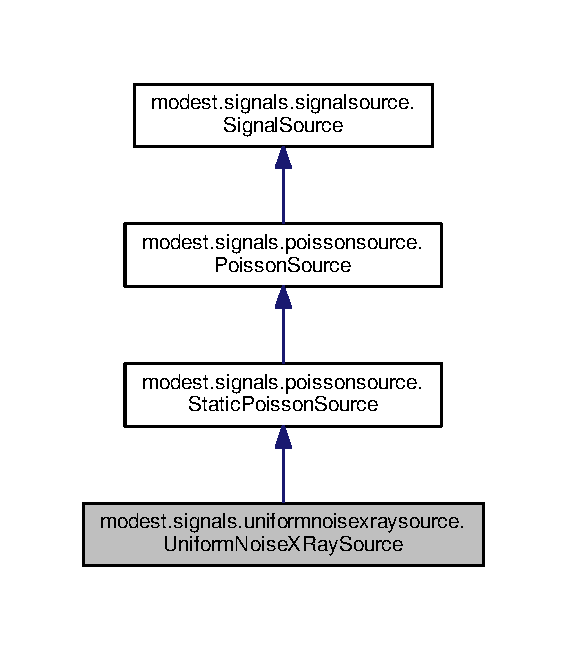
\includegraphics[width=272pt]{classmodest_1_1signals_1_1uniformnoisexraysource_1_1UniformNoiseXRaySource__inherit__graph}
\end{center}
\end{figure}


Collaboration diagram for modest.\+signals.\+uniformnoisexraysource.\+Uniform\+Noise\+X\+Ray\+Source\+:
\nopagebreak
\begin{figure}[H]
\begin{center}
\leavevmode
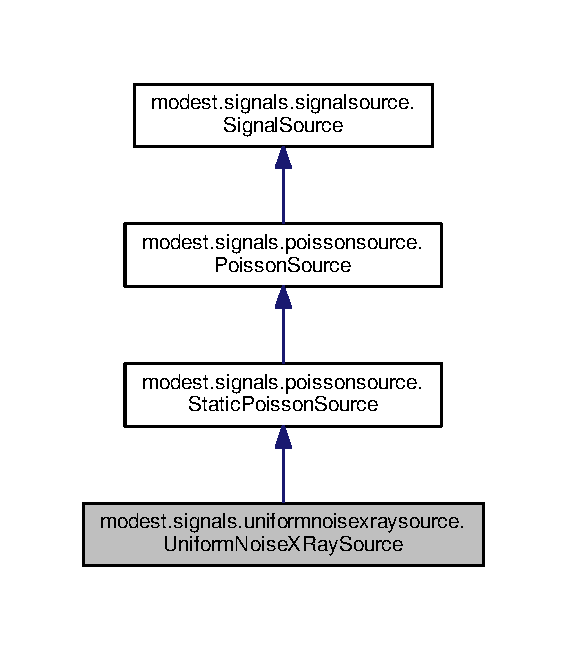
\includegraphics[width=272pt]{classmodest_1_1signals_1_1uniformnoisexraysource_1_1UniformNoiseXRaySource__coll__graph}
\end{center}
\end{figure}
\subsection*{Public Member Functions}
\begin{DoxyCompactItemize}
\item 
def \hyperlink{classmodest_1_1signals_1_1uniformnoisexraysource_1_1UniformNoiseXRaySource_a123b4289c31ce2a595aef68bc940de32}{\+\_\+\+\_\+init\+\_\+\+\_\+} (self, \hyperlink{classmodest_1_1signals_1_1uniformnoisexraysource_1_1UniformNoiseXRaySource_a0f958a631c21f5e56d09e1906a50aa18}{photon\+Flux}=None, energy\+Range\+KeV=\mbox{[}2, detector\+F\+OV=180, \hyperlink{classmodest_1_1signals_1_1uniformnoisexraysource_1_1UniformNoiseXRaySource_a77090ba977ae75035e7d17b1ae458944}{detector\+Area}=1, start\+Time=0)
\item 
def \hyperlink{classmodest_1_1signals_1_1uniformnoisexraysource_1_1UniformNoiseXRaySource_a86a50661bf02e8ca9ffc9df881cc1787}{compute\+Association\+Probability} (self, measurement, state\+Dict, validation\+Threshold=0)
\item 
def \hyperlink{classmodest_1_1signals_1_1uniformnoisexraysource_1_1UniformNoiseXRaySource_a40278f1d8d3399df6dd86f23e55852b7}{generate\+Photon\+Arrivals} (self, t\+Max, t0=0, position=None, attitude=None, \hyperlink{classmodest_1_1signals_1_1uniformnoisexraysource_1_1UniformNoiseXRaySource_a7cfd254af9003d98214119e5d11f226e}{F\+OV}=None, A\+O\+A\+\_\+\+Std\+Dev=None, T\+O\+A\+\_\+\+Std\+Dev=None)
\item 
def \hyperlink{classmodest_1_1signals_1_1uniformnoisexraysource_1_1UniformNoiseXRaySource_ad4c8ce337443a66977e4d2b296ae5e30}{generate\+Uniform\+Arrival\+Vectors} (self, n\+Vectors, \hyperlink{classmodest_1_1signals_1_1uniformnoisexraysource_1_1UniformNoiseXRaySource_a7cfd254af9003d98214119e5d11f226e}{F\+OV}=None)
\item 
def \hyperlink{classmodest_1_1signals_1_1poissonsource_1_1StaticPoissonSource_a1754d94bff46d97817438bab552afef9}{compute\+Association\+Probability} (self, measurement)
\item 
def \hyperlink{classmodest_1_1signals_1_1poissonsource_1_1PoissonSource_a2f8a73e6f51cbdcd0f1e646d6f4d4574}{compute\+Association\+Probability} (self, current\+Flux, measurement)
\item 
def \hyperlink{classmodest_1_1signals_1_1poissonsource_1_1StaticPoissonSource_acc0f087c93d5e90070f4cd0be95ace74}{generate\+Events} (self, t\+Max, t0=0)
\item 
def \hyperlink{classmodest_1_1signals_1_1signalsource_1_1SignalSource_a9a64c6a9c2954f6ad61e4ca3518ea8ab}{signal\+ID} (self)
\end{DoxyCompactItemize}
\subsection*{Public Attributes}
\begin{DoxyCompactItemize}
\item 
\hyperlink{classmodest_1_1signals_1_1uniformnoisexraysource_1_1UniformNoiseXRaySource_a0f958a631c21f5e56d09e1906a50aa18}{photon\+Flux}
\item 
\hyperlink{classmodest_1_1signals_1_1uniformnoisexraysource_1_1UniformNoiseXRaySource_a7cfd254af9003d98214119e5d11f226e}{F\+OV}
\item 
\hyperlink{classmodest_1_1signals_1_1uniformnoisexraysource_1_1UniformNoiseXRaySource_a8cea08a8576dbaaab7da58569eeac3c1}{F\+O\+V\+\_\+\+Solid\+Angle}
\item 
\hyperlink{classmodest_1_1signals_1_1uniformnoisexraysource_1_1UniformNoiseXRaySource_a77090ba977ae75035e7d17b1ae458944}{detector\+Area}
\item 
\hyperlink{classmodest_1_1signals_1_1poissonsource_1_1PoissonSource_a34395fc83bd8743a0a5ee69f9392a606}{last\+Time}
\item 
\hyperlink{classmodest_1_1signals_1_1poissonsource_1_1PoissonSource_a6f2c657ad936b921715d826ac74f7fe5}{flux}
\end{DoxyCompactItemize}
\subsection*{Static Public Attributes}
\begin{DoxyCompactItemize}
\item 
int \hyperlink{classmodest_1_1signals_1_1signalsource_1_1SignalSource_a453eafb550b551adbec0903deb63dfce}{next\+Signal\+ID} = 0
\end{DoxyCompactItemize}


\subsection{Detailed Description}


Definition at line 12 of file uniformnoisexraysource.\+py.



\subsection{Constructor \& Destructor Documentation}
\index{modest\+::signals\+::uniformnoisexraysource\+::\+Uniform\+Noise\+X\+Ray\+Source@{modest\+::signals\+::uniformnoisexraysource\+::\+Uniform\+Noise\+X\+Ray\+Source}!\+\_\+\+\_\+init\+\_\+\+\_\+@{\+\_\+\+\_\+init\+\_\+\+\_\+}}
\index{\+\_\+\+\_\+init\+\_\+\+\_\+@{\+\_\+\+\_\+init\+\_\+\+\_\+}!modest\+::signals\+::uniformnoisexraysource\+::\+Uniform\+Noise\+X\+Ray\+Source@{modest\+::signals\+::uniformnoisexraysource\+::\+Uniform\+Noise\+X\+Ray\+Source}}
\subsubsection[{\texorpdfstring{\+\_\+\+\_\+init\+\_\+\+\_\+(self, photon\+Flux=\+None, energy\+Range\+Ke\+V=[2, detector\+F\+O\+V=180, detector\+Area=1, start\+Time=0)}{__init__(self, photonFlux=None, energyRangeKeV=[2, detectorFOV=180, detectorArea=1, startTime=0)}}]{\setlength{\rightskip}{0pt plus 5cm}def modest.\+signals.\+uniformnoisexraysource.\+Uniform\+Noise\+X\+Ray\+Source.\+\_\+\+\_\+init\+\_\+\+\_\+ (
\begin{DoxyParamCaption}
\item[{}]{self, }
\item[{}]{photon\+Flux = {\ttfamily None}, }
\item[{}]{energy\+Range\+KeV = {\ttfamily \mbox{[}2}, }
\item[{}]{detector\+F\+OV = {\ttfamily 180}, }
\item[{}]{detector\+Area = {\ttfamily 1}, }
\item[{}]{start\+Time = {\ttfamily 0}}
\end{DoxyParamCaption}
)}\hypertarget{classmodest_1_1signals_1_1uniformnoisexraysource_1_1UniformNoiseXRaySource_a123b4289c31ce2a595aef68bc940de32}{}\label{classmodest_1_1signals_1_1uniformnoisexraysource_1_1UniformNoiseXRaySource_a123b4289c31ce2a595aef68bc940de32}


Definition at line 20 of file uniformnoisexraysource.\+py.



\subsection{Member Function Documentation}
\index{modest\+::signals\+::uniformnoisexraysource\+::\+Uniform\+Noise\+X\+Ray\+Source@{modest\+::signals\+::uniformnoisexraysource\+::\+Uniform\+Noise\+X\+Ray\+Source}!compute\+Association\+Probability@{compute\+Association\+Probability}}
\index{compute\+Association\+Probability@{compute\+Association\+Probability}!modest\+::signals\+::uniformnoisexraysource\+::\+Uniform\+Noise\+X\+Ray\+Source@{modest\+::signals\+::uniformnoisexraysource\+::\+Uniform\+Noise\+X\+Ray\+Source}}
\subsubsection[{\texorpdfstring{compute\+Association\+Probability(self, current\+Flux, measurement)}{computeAssociationProbability(self, currentFlux, measurement)}}]{\setlength{\rightskip}{0pt plus 5cm}def modest.\+signals.\+poissonsource.\+Poisson\+Source.\+compute\+Association\+Probability (
\begin{DoxyParamCaption}
\item[{}]{self, }
\item[{}]{current\+Flux, }
\item[{}]{measurement}
\end{DoxyParamCaption}
)\hspace{0.3cm}{\ttfamily [inherited]}}\hypertarget{classmodest_1_1signals_1_1poissonsource_1_1PoissonSource_a2f8a73e6f51cbdcd0f1e646d6f4d4574}{}\label{classmodest_1_1signals_1_1poissonsource_1_1PoissonSource_a2f8a73e6f51cbdcd0f1e646d6f4d4574}


Definition at line 23 of file poissonsource.\+py.

\index{modest\+::signals\+::uniformnoisexraysource\+::\+Uniform\+Noise\+X\+Ray\+Source@{modest\+::signals\+::uniformnoisexraysource\+::\+Uniform\+Noise\+X\+Ray\+Source}!compute\+Association\+Probability@{compute\+Association\+Probability}}
\index{compute\+Association\+Probability@{compute\+Association\+Probability}!modest\+::signals\+::uniformnoisexraysource\+::\+Uniform\+Noise\+X\+Ray\+Source@{modest\+::signals\+::uniformnoisexraysource\+::\+Uniform\+Noise\+X\+Ray\+Source}}
\subsubsection[{\texorpdfstring{compute\+Association\+Probability(self, measurement)}{computeAssociationProbability(self, measurement)}}]{\setlength{\rightskip}{0pt plus 5cm}def modest.\+signals.\+poissonsource.\+Static\+Poisson\+Source.\+compute\+Association\+Probability (
\begin{DoxyParamCaption}
\item[{}]{self, }
\item[{}]{measurement}
\end{DoxyParamCaption}
)\hspace{0.3cm}{\ttfamily [inherited]}}\hypertarget{classmodest_1_1signals_1_1poissonsource_1_1StaticPoissonSource_a1754d94bff46d97817438bab552afef9}{}\label{classmodest_1_1signals_1_1poissonsource_1_1StaticPoissonSource_a1754d94bff46d97817438bab552afef9}


Definition at line 42 of file poissonsource.\+py.

\index{modest\+::signals\+::uniformnoisexraysource\+::\+Uniform\+Noise\+X\+Ray\+Source@{modest\+::signals\+::uniformnoisexraysource\+::\+Uniform\+Noise\+X\+Ray\+Source}!compute\+Association\+Probability@{compute\+Association\+Probability}}
\index{compute\+Association\+Probability@{compute\+Association\+Probability}!modest\+::signals\+::uniformnoisexraysource\+::\+Uniform\+Noise\+X\+Ray\+Source@{modest\+::signals\+::uniformnoisexraysource\+::\+Uniform\+Noise\+X\+Ray\+Source}}
\subsubsection[{\texorpdfstring{compute\+Association\+Probability(self, measurement, state\+Dict, validation\+Threshold=0)}{computeAssociationProbability(self, measurement, stateDict, validationThreshold=0)}}]{\setlength{\rightskip}{0pt plus 5cm}def modest.\+signals.\+uniformnoisexraysource.\+Uniform\+Noise\+X\+Ray\+Source.\+compute\+Association\+Probability (
\begin{DoxyParamCaption}
\item[{}]{self, }
\item[{}]{measurement, }
\item[{}]{state\+Dict, }
\item[{}]{validation\+Threshold = {\ttfamily 0}}
\end{DoxyParamCaption}
)}\hypertarget{classmodest_1_1signals_1_1uniformnoisexraysource_1_1UniformNoiseXRaySource_a86a50661bf02e8ca9ffc9df881cc1787}{}\label{classmodest_1_1signals_1_1uniformnoisexraysource_1_1UniformNoiseXRaySource_a86a50661bf02e8ca9ffc9df881cc1787}


Definition at line 44 of file uniformnoisexraysource.\+py.

\index{modest\+::signals\+::uniformnoisexraysource\+::\+Uniform\+Noise\+X\+Ray\+Source@{modest\+::signals\+::uniformnoisexraysource\+::\+Uniform\+Noise\+X\+Ray\+Source}!generate\+Events@{generate\+Events}}
\index{generate\+Events@{generate\+Events}!modest\+::signals\+::uniformnoisexraysource\+::\+Uniform\+Noise\+X\+Ray\+Source@{modest\+::signals\+::uniformnoisexraysource\+::\+Uniform\+Noise\+X\+Ray\+Source}}
\subsubsection[{\texorpdfstring{generate\+Events(self, t\+Max, t0=0)}{generateEvents(self, tMax, t0=0)}}]{\setlength{\rightskip}{0pt plus 5cm}def modest.\+signals.\+poissonsource.\+Static\+Poisson\+Source.\+generate\+Events (
\begin{DoxyParamCaption}
\item[{}]{self, }
\item[{}]{t\+Max, }
\item[{}]{t0 = {\ttfamily 0}}
\end{DoxyParamCaption}
)\hspace{0.3cm}{\ttfamily [inherited]}}\hypertarget{classmodest_1_1signals_1_1poissonsource_1_1StaticPoissonSource_acc0f087c93d5e90070f4cd0be95ace74}{}\label{classmodest_1_1signals_1_1poissonsource_1_1StaticPoissonSource_acc0f087c93d5e90070f4cd0be95ace74}


Definition at line 53 of file poissonsource.\+py.

\index{modest\+::signals\+::uniformnoisexraysource\+::\+Uniform\+Noise\+X\+Ray\+Source@{modest\+::signals\+::uniformnoisexraysource\+::\+Uniform\+Noise\+X\+Ray\+Source}!generate\+Photon\+Arrivals@{generate\+Photon\+Arrivals}}
\index{generate\+Photon\+Arrivals@{generate\+Photon\+Arrivals}!modest\+::signals\+::uniformnoisexraysource\+::\+Uniform\+Noise\+X\+Ray\+Source@{modest\+::signals\+::uniformnoisexraysource\+::\+Uniform\+Noise\+X\+Ray\+Source}}
\subsubsection[{\texorpdfstring{generate\+Photon\+Arrivals(self, t\+Max, t0=0, position=\+None, attitude=\+None, F\+O\+V=\+None, A\+O\+A\+\_\+\+Std\+Dev=\+None, T\+O\+A\+\_\+\+Std\+Dev=\+None)}{generatePhotonArrivals(self, tMax, t0=0, position=None, attitude=None, FOV=None, AOA_StdDev=None, TOA_StdDev=None)}}]{\setlength{\rightskip}{0pt plus 5cm}def modest.\+signals.\+uniformnoisexraysource.\+Uniform\+Noise\+X\+Ray\+Source.\+generate\+Photon\+Arrivals (
\begin{DoxyParamCaption}
\item[{}]{self, }
\item[{}]{t\+Max, }
\item[{}]{t0 = {\ttfamily 0}, }
\item[{}]{position = {\ttfamily None}, }
\item[{}]{attitude = {\ttfamily None}, }
\item[{}]{F\+OV = {\ttfamily None}, }
\item[{}]{A\+O\+A\+\_\+\+Std\+Dev = {\ttfamily None}, }
\item[{}]{T\+O\+A\+\_\+\+Std\+Dev = {\ttfamily None}}
\end{DoxyParamCaption}
)}\hypertarget{classmodest_1_1signals_1_1uniformnoisexraysource_1_1UniformNoiseXRaySource_a40278f1d8d3399df6dd86f23e55852b7}{}\label{classmodest_1_1signals_1_1uniformnoisexraysource_1_1UniformNoiseXRaySource_a40278f1d8d3399df6dd86f23e55852b7}


Definition at line 69 of file uniformnoisexraysource.\+py.

\index{modest\+::signals\+::uniformnoisexraysource\+::\+Uniform\+Noise\+X\+Ray\+Source@{modest\+::signals\+::uniformnoisexraysource\+::\+Uniform\+Noise\+X\+Ray\+Source}!generate\+Uniform\+Arrival\+Vectors@{generate\+Uniform\+Arrival\+Vectors}}
\index{generate\+Uniform\+Arrival\+Vectors@{generate\+Uniform\+Arrival\+Vectors}!modest\+::signals\+::uniformnoisexraysource\+::\+Uniform\+Noise\+X\+Ray\+Source@{modest\+::signals\+::uniformnoisexraysource\+::\+Uniform\+Noise\+X\+Ray\+Source}}
\subsubsection[{\texorpdfstring{generate\+Uniform\+Arrival\+Vectors(self, n\+Vectors, F\+O\+V=\+None)}{generateUniformArrivalVectors(self, nVectors, FOV=None)}}]{\setlength{\rightskip}{0pt plus 5cm}def modest.\+signals.\+uniformnoisexraysource.\+Uniform\+Noise\+X\+Ray\+Source.\+generate\+Uniform\+Arrival\+Vectors (
\begin{DoxyParamCaption}
\item[{}]{self, }
\item[{}]{n\+Vectors, }
\item[{}]{F\+OV = {\ttfamily None}}
\end{DoxyParamCaption}
)}\hypertarget{classmodest_1_1signals_1_1uniformnoisexraysource_1_1UniformNoiseXRaySource_ad4c8ce337443a66977e4d2b296ae5e30}{}\label{classmodest_1_1signals_1_1uniformnoisexraysource_1_1UniformNoiseXRaySource_ad4c8ce337443a66977e4d2b296ae5e30}


Definition at line 114 of file uniformnoisexraysource.\+py.

\index{modest\+::signals\+::uniformnoisexraysource\+::\+Uniform\+Noise\+X\+Ray\+Source@{modest\+::signals\+::uniformnoisexraysource\+::\+Uniform\+Noise\+X\+Ray\+Source}!signal\+ID@{signal\+ID}}
\index{signal\+ID@{signal\+ID}!modest\+::signals\+::uniformnoisexraysource\+::\+Uniform\+Noise\+X\+Ray\+Source@{modest\+::signals\+::uniformnoisexraysource\+::\+Uniform\+Noise\+X\+Ray\+Source}}
\subsubsection[{\texorpdfstring{signal\+I\+D(self)}{signalID(self)}}]{\setlength{\rightskip}{0pt plus 5cm}def modest.\+signals.\+signalsource.\+Signal\+Source.\+signal\+ID (
\begin{DoxyParamCaption}
\item[{}]{self}
\end{DoxyParamCaption}
)\hspace{0.3cm}{\ttfamily [inherited]}}\hypertarget{classmodest_1_1signals_1_1signalsource_1_1SignalSource_a9a64c6a9c2954f6ad61e4ca3518ea8ab}{}\label{classmodest_1_1signals_1_1signalsource_1_1SignalSource_a9a64c6a9c2954f6ad61e4ca3518ea8ab}


Definition at line 17 of file signalsource.\+py.



\subsection{Member Data Documentation}
\index{modest\+::signals\+::uniformnoisexraysource\+::\+Uniform\+Noise\+X\+Ray\+Source@{modest\+::signals\+::uniformnoisexraysource\+::\+Uniform\+Noise\+X\+Ray\+Source}!detector\+Area@{detector\+Area}}
\index{detector\+Area@{detector\+Area}!modest\+::signals\+::uniformnoisexraysource\+::\+Uniform\+Noise\+X\+Ray\+Source@{modest\+::signals\+::uniformnoisexraysource\+::\+Uniform\+Noise\+X\+Ray\+Source}}
\subsubsection[{\texorpdfstring{detector\+Area}{detectorArea}}]{\setlength{\rightskip}{0pt plus 5cm}modest.\+signals.\+uniformnoisexraysource.\+Uniform\+Noise\+X\+Ray\+Source.\+detector\+Area}\hypertarget{classmodest_1_1signals_1_1uniformnoisexraysource_1_1UniformNoiseXRaySource_a77090ba977ae75035e7d17b1ae458944}{}\label{classmodest_1_1signals_1_1uniformnoisexraysource_1_1UniformNoiseXRaySource_a77090ba977ae75035e7d17b1ae458944}


Definition at line 34 of file uniformnoisexraysource.\+py.

\index{modest\+::signals\+::uniformnoisexraysource\+::\+Uniform\+Noise\+X\+Ray\+Source@{modest\+::signals\+::uniformnoisexraysource\+::\+Uniform\+Noise\+X\+Ray\+Source}!flux@{flux}}
\index{flux@{flux}!modest\+::signals\+::uniformnoisexraysource\+::\+Uniform\+Noise\+X\+Ray\+Source@{modest\+::signals\+::uniformnoisexraysource\+::\+Uniform\+Noise\+X\+Ray\+Source}}
\subsubsection[{\texorpdfstring{flux}{flux}}]{\setlength{\rightskip}{0pt plus 5cm}modest.\+signals.\+poissonsource.\+Poisson\+Source.\+flux\hspace{0.3cm}{\ttfamily [inherited]}}\hypertarget{classmodest_1_1signals_1_1poissonsource_1_1PoissonSource_a6f2c657ad936b921715d826ac74f7fe5}{}\label{classmodest_1_1signals_1_1poissonsource_1_1PoissonSource_a6f2c657ad936b921715d826ac74f7fe5}


Definition at line 16 of file poissonsource.\+py.

\index{modest\+::signals\+::uniformnoisexraysource\+::\+Uniform\+Noise\+X\+Ray\+Source@{modest\+::signals\+::uniformnoisexraysource\+::\+Uniform\+Noise\+X\+Ray\+Source}!F\+OV@{F\+OV}}
\index{F\+OV@{F\+OV}!modest\+::signals\+::uniformnoisexraysource\+::\+Uniform\+Noise\+X\+Ray\+Source@{modest\+::signals\+::uniformnoisexraysource\+::\+Uniform\+Noise\+X\+Ray\+Source}}
\subsubsection[{\texorpdfstring{F\+OV}{FOV}}]{\setlength{\rightskip}{0pt plus 5cm}modest.\+signals.\+uniformnoisexraysource.\+Uniform\+Noise\+X\+Ray\+Source.\+F\+OV}\hypertarget{classmodest_1_1signals_1_1uniformnoisexraysource_1_1UniformNoiseXRaySource_a7cfd254af9003d98214119e5d11f226e}{}\label{classmodest_1_1signals_1_1uniformnoisexraysource_1_1UniformNoiseXRaySource_a7cfd254af9003d98214119e5d11f226e}


Definition at line 32 of file uniformnoisexraysource.\+py.

\index{modest\+::signals\+::uniformnoisexraysource\+::\+Uniform\+Noise\+X\+Ray\+Source@{modest\+::signals\+::uniformnoisexraysource\+::\+Uniform\+Noise\+X\+Ray\+Source}!F\+O\+V\+\_\+\+Solid\+Angle@{F\+O\+V\+\_\+\+Solid\+Angle}}
\index{F\+O\+V\+\_\+\+Solid\+Angle@{F\+O\+V\+\_\+\+Solid\+Angle}!modest\+::signals\+::uniformnoisexraysource\+::\+Uniform\+Noise\+X\+Ray\+Source@{modest\+::signals\+::uniformnoisexraysource\+::\+Uniform\+Noise\+X\+Ray\+Source}}
\subsubsection[{\texorpdfstring{F\+O\+V\+\_\+\+Solid\+Angle}{FOV_SolidAngle}}]{\setlength{\rightskip}{0pt plus 5cm}modest.\+signals.\+uniformnoisexraysource.\+Uniform\+Noise\+X\+Ray\+Source.\+F\+O\+V\+\_\+\+Solid\+Angle}\hypertarget{classmodest_1_1signals_1_1uniformnoisexraysource_1_1UniformNoiseXRaySource_a8cea08a8576dbaaab7da58569eeac3c1}{}\label{classmodest_1_1signals_1_1uniformnoisexraysource_1_1UniformNoiseXRaySource_a8cea08a8576dbaaab7da58569eeac3c1}


Definition at line 33 of file uniformnoisexraysource.\+py.

\index{modest\+::signals\+::uniformnoisexraysource\+::\+Uniform\+Noise\+X\+Ray\+Source@{modest\+::signals\+::uniformnoisexraysource\+::\+Uniform\+Noise\+X\+Ray\+Source}!last\+Time@{last\+Time}}
\index{last\+Time@{last\+Time}!modest\+::signals\+::uniformnoisexraysource\+::\+Uniform\+Noise\+X\+Ray\+Source@{modest\+::signals\+::uniformnoisexraysource\+::\+Uniform\+Noise\+X\+Ray\+Source}}
\subsubsection[{\texorpdfstring{last\+Time}{lastTime}}]{\setlength{\rightskip}{0pt plus 5cm}modest.\+signals.\+poissonsource.\+Poisson\+Source.\+last\+Time\hspace{0.3cm}{\ttfamily [inherited]}}\hypertarget{classmodest_1_1signals_1_1poissonsource_1_1PoissonSource_a34395fc83bd8743a0a5ee69f9392a606}{}\label{classmodest_1_1signals_1_1poissonsource_1_1PoissonSource_a34395fc83bd8743a0a5ee69f9392a606}


Definition at line 15 of file poissonsource.\+py.

\index{modest\+::signals\+::uniformnoisexraysource\+::\+Uniform\+Noise\+X\+Ray\+Source@{modest\+::signals\+::uniformnoisexraysource\+::\+Uniform\+Noise\+X\+Ray\+Source}!next\+Signal\+ID@{next\+Signal\+ID}}
\index{next\+Signal\+ID@{next\+Signal\+ID}!modest\+::signals\+::uniformnoisexraysource\+::\+Uniform\+Noise\+X\+Ray\+Source@{modest\+::signals\+::uniformnoisexraysource\+::\+Uniform\+Noise\+X\+Ray\+Source}}
\subsubsection[{\texorpdfstring{next\+Signal\+ID}{nextSignalID}}]{\setlength{\rightskip}{0pt plus 5cm}int modest.\+signals.\+signalsource.\+Signal\+Source.\+next\+Signal\+ID = 0\hspace{0.3cm}{\ttfamily [static]}, {\ttfamily [inherited]}}\hypertarget{classmodest_1_1signals_1_1signalsource_1_1SignalSource_a453eafb550b551adbec0903deb63dfce}{}\label{classmodest_1_1signals_1_1signalsource_1_1SignalSource_a453eafb550b551adbec0903deb63dfce}


Definition at line 8 of file signalsource.\+py.

\index{modest\+::signals\+::uniformnoisexraysource\+::\+Uniform\+Noise\+X\+Ray\+Source@{modest\+::signals\+::uniformnoisexraysource\+::\+Uniform\+Noise\+X\+Ray\+Source}!photon\+Flux@{photon\+Flux}}
\index{photon\+Flux@{photon\+Flux}!modest\+::signals\+::uniformnoisexraysource\+::\+Uniform\+Noise\+X\+Ray\+Source@{modest\+::signals\+::uniformnoisexraysource\+::\+Uniform\+Noise\+X\+Ray\+Source}}
\subsubsection[{\texorpdfstring{photon\+Flux}{photonFlux}}]{\setlength{\rightskip}{0pt plus 5cm}modest.\+signals.\+uniformnoisexraysource.\+Uniform\+Noise\+X\+Ray\+Source.\+photon\+Flux}\hypertarget{classmodest_1_1signals_1_1uniformnoisexraysource_1_1UniformNoiseXRaySource_a0f958a631c21f5e56d09e1906a50aa18}{}\label{classmodest_1_1signals_1_1uniformnoisexraysource_1_1UniformNoiseXRaySource_a0f958a631c21f5e56d09e1906a50aa18}


Definition at line 22 of file uniformnoisexraysource.\+py.



The documentation for this class was generated from the following file\+:\begin{DoxyCompactItemize}
\item 
modest/signals/\hyperlink{uniformnoisexraysource_8py}{uniformnoisexraysource.\+py}\end{DoxyCompactItemize}

\hypertarget{classmodest_1_1signals_1_1xraysource_1_1UniformNoiseXRaySource}{}\section{modest.\+signals.\+xraysource.\+Uniform\+Noise\+X\+Ray\+Source Class Reference}
\label{classmodest_1_1signals_1_1xraysource_1_1UniformNoiseXRaySource}\index{modest.\+signals.\+xraysource.\+Uniform\+Noise\+X\+Ray\+Source@{modest.\+signals.\+xraysource.\+Uniform\+Noise\+X\+Ray\+Source}}


Inheritance diagram for modest.\+signals.\+xraysource.\+Uniform\+Noise\+X\+Ray\+Source\+:\nopagebreak
\begin{figure}[H]
\begin{center}
\leavevmode
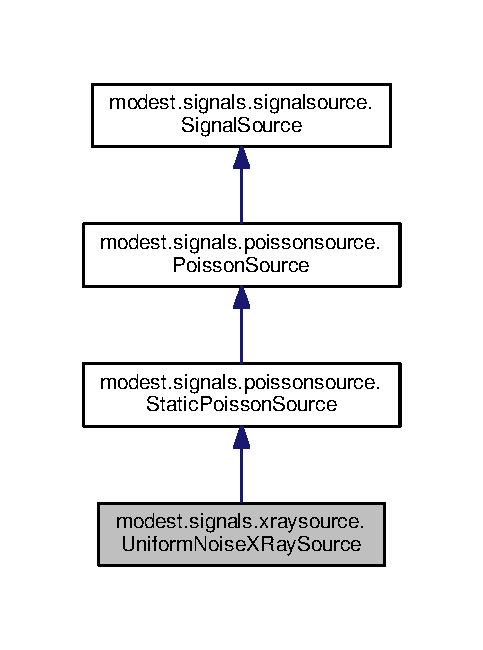
\includegraphics[width=232pt]{classmodest_1_1signals_1_1xraysource_1_1UniformNoiseXRaySource__inherit__graph}
\end{center}
\end{figure}


Collaboration diagram for modest.\+signals.\+xraysource.\+Uniform\+Noise\+X\+Ray\+Source\+:\nopagebreak
\begin{figure}[H]
\begin{center}
\leavevmode
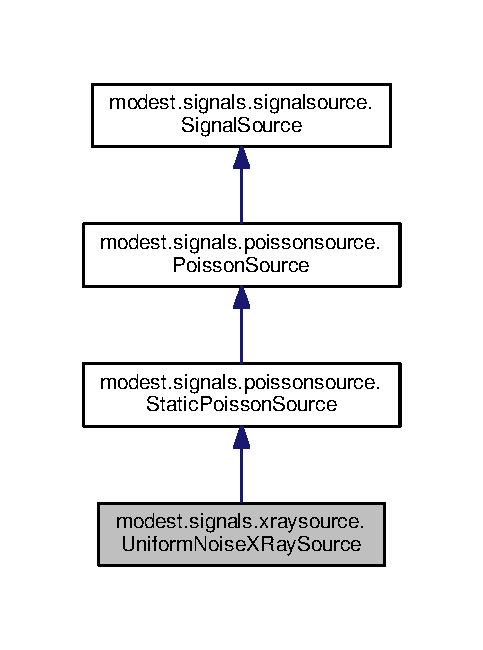
\includegraphics[width=232pt]{classmodest_1_1signals_1_1xraysource_1_1UniformNoiseXRaySource__coll__graph}
\end{center}
\end{figure}
\subsection*{Public Member Functions}
\begin{DoxyCompactItemize}
\item 
def \hyperlink{classmodest_1_1signals_1_1xraysource_1_1UniformNoiseXRaySource_a2bf2964e92d4540de35c6eebfe4944db}{\+\_\+\+\_\+init\+\_\+\+\_\+} (self, \hyperlink{classmodest_1_1signals_1_1xraysource_1_1UniformNoiseXRaySource_a9b8049972baf6e0640181b58850a3d20}{photon\+Flux})
\item 
def \hyperlink{classmodest_1_1signals_1_1xraysource_1_1UniformNoiseXRaySource_aa4732c82202fd8c607ae0f8244be3272}{compute\+Association\+Probability} (self, measurement, state\+Dict, validation\+Threshold=0)
\item 
def \hyperlink{classmodest_1_1signals_1_1poissonsource_1_1StaticPoissonSource_a1754d94bff46d97817438bab552afef9}{compute\+Association\+Probability} (self, measurement)
\item 
def \hyperlink{classmodest_1_1signals_1_1poissonsource_1_1PoissonSource_a2f8a73e6f51cbdcd0f1e646d6f4d4574}{compute\+Association\+Probability} (self, current\+Flux, measurement)
\item 
def \hyperlink{classmodest_1_1signals_1_1signalsource_1_1SignalSource_a9a64c6a9c2954f6ad61e4ca3518ea8ab}{signal\+ID} (self)
\end{DoxyCompactItemize}
\subsection*{Public Attributes}
\begin{DoxyCompactItemize}
\item 
\hyperlink{classmodest_1_1signals_1_1xraysource_1_1UniformNoiseXRaySource_a9b8049972baf6e0640181b58850a3d20}{photon\+Flux}
\item 
\hyperlink{classmodest_1_1signals_1_1poissonsource_1_1PoissonSource_a34395fc83bd8743a0a5ee69f9392a606}{last\+Time}
\item 
\hyperlink{classmodest_1_1signals_1_1poissonsource_1_1PoissonSource_a6f2c657ad936b921715d826ac74f7fe5}{flux}
\end{DoxyCompactItemize}
\subsection*{Static Public Attributes}
\begin{DoxyCompactItemize}
\item 
int \hyperlink{classmodest_1_1signals_1_1signalsource_1_1SignalSource_a453eafb550b551adbec0903deb63dfce}{next\+Signal\+ID} = 0
\end{DoxyCompactItemize}


\subsection{Detailed Description}


Definition at line 43 of file xraysource.\+py.



\subsection{Constructor \& Destructor Documentation}
\index{modest\+::signals\+::xraysource\+::\+Uniform\+Noise\+X\+Ray\+Source@{modest\+::signals\+::xraysource\+::\+Uniform\+Noise\+X\+Ray\+Source}!\+\_\+\+\_\+init\+\_\+\+\_\+@{\+\_\+\+\_\+init\+\_\+\+\_\+}}
\index{\+\_\+\+\_\+init\+\_\+\+\_\+@{\+\_\+\+\_\+init\+\_\+\+\_\+}!modest\+::signals\+::xraysource\+::\+Uniform\+Noise\+X\+Ray\+Source@{modest\+::signals\+::xraysource\+::\+Uniform\+Noise\+X\+Ray\+Source}}
\subsubsection[{\texorpdfstring{\+\_\+\+\_\+init\+\_\+\+\_\+(self, photon\+Flux)}{__init__(self, photonFlux)}}]{\setlength{\rightskip}{0pt plus 5cm}def modest.\+signals.\+xraysource.\+Uniform\+Noise\+X\+Ray\+Source.\+\_\+\+\_\+init\+\_\+\+\_\+ (
\begin{DoxyParamCaption}
\item[{}]{self, }
\item[{}]{photon\+Flux}
\end{DoxyParamCaption}
)}\hypertarget{classmodest_1_1signals_1_1xraysource_1_1UniformNoiseXRaySource_a2bf2964e92d4540de35c6eebfe4944db}{}\label{classmodest_1_1signals_1_1xraysource_1_1UniformNoiseXRaySource_a2bf2964e92d4540de35c6eebfe4944db}


Definition at line 47 of file xraysource.\+py.



\subsection{Member Function Documentation}
\index{modest\+::signals\+::xraysource\+::\+Uniform\+Noise\+X\+Ray\+Source@{modest\+::signals\+::xraysource\+::\+Uniform\+Noise\+X\+Ray\+Source}!compute\+Association\+Probability@{compute\+Association\+Probability}}
\index{compute\+Association\+Probability@{compute\+Association\+Probability}!modest\+::signals\+::xraysource\+::\+Uniform\+Noise\+X\+Ray\+Source@{modest\+::signals\+::xraysource\+::\+Uniform\+Noise\+X\+Ray\+Source}}
\subsubsection[{\texorpdfstring{compute\+Association\+Probability(self, current\+Flux, measurement)}{computeAssociationProbability(self, currentFlux, measurement)}}]{\setlength{\rightskip}{0pt plus 5cm}def modest.\+signals.\+poissonsource.\+Poisson\+Source.\+compute\+Association\+Probability (
\begin{DoxyParamCaption}
\item[{}]{self, }
\item[{}]{current\+Flux, }
\item[{}]{measurement}
\end{DoxyParamCaption}
)\hspace{0.3cm}{\ttfamily [inherited]}}\hypertarget{classmodest_1_1signals_1_1poissonsource_1_1PoissonSource_a2f8a73e6f51cbdcd0f1e646d6f4d4574}{}\label{classmodest_1_1signals_1_1poissonsource_1_1PoissonSource_a2f8a73e6f51cbdcd0f1e646d6f4d4574}


Definition at line 20 of file poissonsource.\+py.

\index{modest\+::signals\+::xraysource\+::\+Uniform\+Noise\+X\+Ray\+Source@{modest\+::signals\+::xraysource\+::\+Uniform\+Noise\+X\+Ray\+Source}!compute\+Association\+Probability@{compute\+Association\+Probability}}
\index{compute\+Association\+Probability@{compute\+Association\+Probability}!modest\+::signals\+::xraysource\+::\+Uniform\+Noise\+X\+Ray\+Source@{modest\+::signals\+::xraysource\+::\+Uniform\+Noise\+X\+Ray\+Source}}
\subsubsection[{\texorpdfstring{compute\+Association\+Probability(self, measurement)}{computeAssociationProbability(self, measurement)}}]{\setlength{\rightskip}{0pt plus 5cm}def modest.\+signals.\+poissonsource.\+Static\+Poisson\+Source.\+compute\+Association\+Probability (
\begin{DoxyParamCaption}
\item[{}]{self, }
\item[{}]{measurement}
\end{DoxyParamCaption}
)\hspace{0.3cm}{\ttfamily [inherited]}}\hypertarget{classmodest_1_1signals_1_1poissonsource_1_1StaticPoissonSource_a1754d94bff46d97817438bab552afef9}{}\label{classmodest_1_1signals_1_1poissonsource_1_1StaticPoissonSource_a1754d94bff46d97817438bab552afef9}


Definition at line 37 of file poissonsource.\+py.

\index{modest\+::signals\+::xraysource\+::\+Uniform\+Noise\+X\+Ray\+Source@{modest\+::signals\+::xraysource\+::\+Uniform\+Noise\+X\+Ray\+Source}!compute\+Association\+Probability@{compute\+Association\+Probability}}
\index{compute\+Association\+Probability@{compute\+Association\+Probability}!modest\+::signals\+::xraysource\+::\+Uniform\+Noise\+X\+Ray\+Source@{modest\+::signals\+::xraysource\+::\+Uniform\+Noise\+X\+Ray\+Source}}
\subsubsection[{\texorpdfstring{compute\+Association\+Probability(self, measurement, state\+Dict, validation\+Threshold=0)}{computeAssociationProbability(self, measurement, stateDict, validationThreshold=0)}}]{\setlength{\rightskip}{0pt plus 5cm}def modest.\+signals.\+xraysource.\+Uniform\+Noise\+X\+Ray\+Source.\+compute\+Association\+Probability (
\begin{DoxyParamCaption}
\item[{}]{self, }
\item[{}]{measurement, }
\item[{}]{state\+Dict, }
\item[{}]{validation\+Threshold = {\ttfamily 0}}
\end{DoxyParamCaption}
)}\hypertarget{classmodest_1_1signals_1_1xraysource_1_1UniformNoiseXRaySource_aa4732c82202fd8c607ae0f8244be3272}{}\label{classmodest_1_1signals_1_1xraysource_1_1UniformNoiseXRaySource_aa4732c82202fd8c607ae0f8244be3272}


Definition at line 58 of file xraysource.\+py.

\index{modest\+::signals\+::xraysource\+::\+Uniform\+Noise\+X\+Ray\+Source@{modest\+::signals\+::xraysource\+::\+Uniform\+Noise\+X\+Ray\+Source}!signal\+ID@{signal\+ID}}
\index{signal\+ID@{signal\+ID}!modest\+::signals\+::xraysource\+::\+Uniform\+Noise\+X\+Ray\+Source@{modest\+::signals\+::xraysource\+::\+Uniform\+Noise\+X\+Ray\+Source}}
\subsubsection[{\texorpdfstring{signal\+I\+D(self)}{signalID(self)}}]{\setlength{\rightskip}{0pt plus 5cm}def modest.\+signals.\+signalsource.\+Signal\+Source.\+signal\+ID (
\begin{DoxyParamCaption}
\item[{}]{self}
\end{DoxyParamCaption}
)\hspace{0.3cm}{\ttfamily [inherited]}}\hypertarget{classmodest_1_1signals_1_1signalsource_1_1SignalSource_a9a64c6a9c2954f6ad61e4ca3518ea8ab}{}\label{classmodest_1_1signals_1_1signalsource_1_1SignalSource_a9a64c6a9c2954f6ad61e4ca3518ea8ab}


Definition at line 14 of file signalsource.\+py.



\subsection{Member Data Documentation}
\index{modest\+::signals\+::xraysource\+::\+Uniform\+Noise\+X\+Ray\+Source@{modest\+::signals\+::xraysource\+::\+Uniform\+Noise\+X\+Ray\+Source}!flux@{flux}}
\index{flux@{flux}!modest\+::signals\+::xraysource\+::\+Uniform\+Noise\+X\+Ray\+Source@{modest\+::signals\+::xraysource\+::\+Uniform\+Noise\+X\+Ray\+Source}}
\subsubsection[{\texorpdfstring{flux}{flux}}]{\setlength{\rightskip}{0pt plus 5cm}modest.\+signals.\+poissonsource.\+Poisson\+Source.\+flux\hspace{0.3cm}{\ttfamily [inherited]}}\hypertarget{classmodest_1_1signals_1_1poissonsource_1_1PoissonSource_a6f2c657ad936b921715d826ac74f7fe5}{}\label{classmodest_1_1signals_1_1poissonsource_1_1PoissonSource_a6f2c657ad936b921715d826ac74f7fe5}


Definition at line 13 of file poissonsource.\+py.

\index{modest\+::signals\+::xraysource\+::\+Uniform\+Noise\+X\+Ray\+Source@{modest\+::signals\+::xraysource\+::\+Uniform\+Noise\+X\+Ray\+Source}!last\+Time@{last\+Time}}
\index{last\+Time@{last\+Time}!modest\+::signals\+::xraysource\+::\+Uniform\+Noise\+X\+Ray\+Source@{modest\+::signals\+::xraysource\+::\+Uniform\+Noise\+X\+Ray\+Source}}
\subsubsection[{\texorpdfstring{last\+Time}{lastTime}}]{\setlength{\rightskip}{0pt plus 5cm}modest.\+signals.\+poissonsource.\+Poisson\+Source.\+last\+Time\hspace{0.3cm}{\ttfamily [inherited]}}\hypertarget{classmodest_1_1signals_1_1poissonsource_1_1PoissonSource_a34395fc83bd8743a0a5ee69f9392a606}{}\label{classmodest_1_1signals_1_1poissonsource_1_1PoissonSource_a34395fc83bd8743a0a5ee69f9392a606}


Definition at line 12 of file poissonsource.\+py.

\index{modest\+::signals\+::xraysource\+::\+Uniform\+Noise\+X\+Ray\+Source@{modest\+::signals\+::xraysource\+::\+Uniform\+Noise\+X\+Ray\+Source}!next\+Signal\+ID@{next\+Signal\+ID}}
\index{next\+Signal\+ID@{next\+Signal\+ID}!modest\+::signals\+::xraysource\+::\+Uniform\+Noise\+X\+Ray\+Source@{modest\+::signals\+::xraysource\+::\+Uniform\+Noise\+X\+Ray\+Source}}
\subsubsection[{\texorpdfstring{next\+Signal\+ID}{nextSignalID}}]{\setlength{\rightskip}{0pt plus 5cm}int modest.\+signals.\+signalsource.\+Signal\+Source.\+next\+Signal\+ID = 0\hspace{0.3cm}{\ttfamily [static]}, {\ttfamily [inherited]}}\hypertarget{classmodest_1_1signals_1_1signalsource_1_1SignalSource_a453eafb550b551adbec0903deb63dfce}{}\label{classmodest_1_1signals_1_1signalsource_1_1SignalSource_a453eafb550b551adbec0903deb63dfce}


Definition at line 5 of file signalsource.\+py.

\index{modest\+::signals\+::xraysource\+::\+Uniform\+Noise\+X\+Ray\+Source@{modest\+::signals\+::xraysource\+::\+Uniform\+Noise\+X\+Ray\+Source}!photon\+Flux@{photon\+Flux}}
\index{photon\+Flux@{photon\+Flux}!modest\+::signals\+::xraysource\+::\+Uniform\+Noise\+X\+Ray\+Source@{modest\+::signals\+::xraysource\+::\+Uniform\+Noise\+X\+Ray\+Source}}
\subsubsection[{\texorpdfstring{photon\+Flux}{photonFlux}}]{\setlength{\rightskip}{0pt plus 5cm}modest.\+signals.\+xraysource.\+Uniform\+Noise\+X\+Ray\+Source.\+photon\+Flux}\hypertarget{classmodest_1_1signals_1_1xraysource_1_1UniformNoiseXRaySource_a9b8049972baf6e0640181b58850a3d20}{}\label{classmodest_1_1signals_1_1xraysource_1_1UniformNoiseXRaySource_a9b8049972baf6e0640181b58850a3d20}


Definition at line 50 of file xraysource.\+py.



The documentation for this class was generated from the following file\+:\begin{DoxyCompactItemize}
\item 
modest/signals/\hyperlink{xraysource_8py}{xraysource.\+py}\end{DoxyCompactItemize}

\chapter{File Documentation}
\hypertarget{____init_____8py}{}\section{modest/\+\_\+\+\_\+init\+\_\+\+\_\+.py File Reference}
\label{____init_____8py}\index{modest/\+\_\+\+\_\+init\+\_\+\+\_\+.\+py@{modest/\+\_\+\+\_\+init\+\_\+\+\_\+.\+py}}
\subsection*{Namespaces}
\begin{DoxyCompactItemize}
\item 
 \hyperlink{namespacemodest}{modest}
\end{DoxyCompactItemize}
\subsection*{Variables}
\begin{DoxyCompactItemize}
\item 
list \hyperlink{namespacemodest_a8c36cd07da61d6f2919f708a59f575a7}{modest.\+\_\+\+\_\+all\+\_\+\+\_\+}
\end{DoxyCompactItemize}

\hypertarget{plots_2____init_____8py}{}\section{modest/plots/\+\_\+\+\_\+init\+\_\+\+\_\+.py File Reference}
\label{plots_2____init_____8py}\index{modest/plots/\+\_\+\+\_\+init\+\_\+\+\_\+.\+py@{modest/plots/\+\_\+\+\_\+init\+\_\+\+\_\+.\+py}}
\subsection*{Namespaces}
\begin{DoxyCompactItemize}
\item 
 \hyperlink{namespacemodest_1_1plots}{modest.\+plots}
\end{DoxyCompactItemize}
\subsection*{Variables}
\begin{DoxyCompactItemize}
\item 
list \hyperlink{namespacemodest_1_1plots_aedbfdd69674be9bdda4c778bffbbeae2}{modest.\+plots.\+\_\+\+\_\+all\+\_\+\+\_\+}
\end{DoxyCompactItemize}

\hypertarget{signals_2____init_____8py}{}\section{modest/signals/\+\_\+\+\_\+init\+\_\+\+\_\+.py File Reference}
\label{signals_2____init_____8py}\index{modest/signals/\+\_\+\+\_\+init\+\_\+\+\_\+.\+py@{modest/signals/\+\_\+\+\_\+init\+\_\+\+\_\+.\+py}}
\subsection*{Namespaces}
\begin{DoxyCompactItemize}
\item 
 \hyperlink{namespacemodest_1_1signals}{modest.\+signals}
\end{DoxyCompactItemize}
\subsection*{Variables}
\begin{DoxyCompactItemize}
\item 
list \hyperlink{namespacemodest_1_1signals_aa31151680eba696b8f6eb7877a67adac}{modest.\+signals.\+\_\+\+\_\+all\+\_\+\+\_\+}
\end{DoxyCompactItemize}

\hypertarget{spacecraft_2____init_____8py}{}\section{modest/spacecraft/\+\_\+\+\_\+init\+\_\+\+\_\+.py File Reference}
\label{spacecraft_2____init_____8py}\index{modest/spacecraft/\+\_\+\+\_\+init\+\_\+\+\_\+.\+py@{modest/spacecraft/\+\_\+\+\_\+init\+\_\+\+\_\+.\+py}}
\subsection*{Namespaces}
\begin{DoxyCompactItemize}
\item 
 \hyperlink{namespacemodest_1_1spacecraft}{modest.\+spacecraft}
\end{DoxyCompactItemize}
\subsection*{Variables}
\begin{DoxyCompactItemize}
\item 
list \hyperlink{namespacemodest_1_1spacecraft_a75dc3ff9c9f0072247d38063ad9e1914}{modest.\+spacecraft.\+\_\+\+\_\+all\+\_\+\+\_\+}
\end{DoxyCompactItemize}

\hypertarget{substates_2____init_____8py}{}\section{modest/substates/\+\_\+\+\_\+init\+\_\+\+\_\+.py File Reference}
\label{substates_2____init_____8py}\index{modest/substates/\+\_\+\+\_\+init\+\_\+\+\_\+.\+py@{modest/substates/\+\_\+\+\_\+init\+\_\+\+\_\+.\+py}}
\subsection*{Namespaces}
\begin{DoxyCompactItemize}
\item 
 \hyperlink{namespacemodest_1_1substates}{modest.\+substates}
\end{DoxyCompactItemize}

\hypertarget{utils_2____init_____8py}{}\section{modest/utils/\+\_\+\+\_\+init\+\_\+\+\_\+.py File Reference}
\label{utils_2____init_____8py}\index{modest/utils/\+\_\+\+\_\+init\+\_\+\+\_\+.\+py@{modest/utils/\+\_\+\+\_\+init\+\_\+\+\_\+.\+py}}
\subsection*{Namespaces}
\begin{DoxyCompactItemize}
\item 
 \hyperlink{namespacemodest_1_1utils}{modest.\+utils}
\end{DoxyCompactItemize}
\subsection*{Variables}
\begin{DoxyCompactItemize}
\item 
list \hyperlink{namespacemodest_1_1utils_acd9a8b6ab3a03ab38f1c184c44fb92cb}{modest.\+utils.\+\_\+\+\_\+all\+\_\+\+\_\+}
\end{DoxyCompactItemize}

\hypertarget{modularfilter_8py}{}\section{modest/modularfilter.py File Reference}
\label{modularfilter_8py}\index{modest/modularfilter.\+py@{modest/modularfilter.\+py}}
\subsection*{Classes}
\begin{DoxyCompactItemize}
\item 
class \hyperlink{classmodest_1_1modularfilter_1_1ModularFilter}{modest.\+modularfilter.\+Modular\+Filter}
\end{DoxyCompactItemize}
\subsection*{Namespaces}
\begin{DoxyCompactItemize}
\item 
 \hyperlink{namespacemodest_1_1modularfilter}{modest.\+modularfilter}
\item 
 \hyperlink{namespaceState}{State}
\begin{DoxyCompactList}\small\item\em This package contains the Modular\+Filter class. \end{DoxyCompactList}\end{DoxyCompactItemize}

\hypertarget{montecarloplots_8py}{}\section{modest/plots/montecarloplots.py File Reference}
\label{montecarloplots_8py}\index{modest/plots/montecarloplots.\+py@{modest/plots/montecarloplots.\+py}}
\subsection*{Namespaces}
\begin{DoxyCompactItemize}
\item 
 \hyperlink{namespacemodest_1_1plots_1_1montecarloplots}{modest.\+plots.\+montecarloplots}
\end{DoxyCompactItemize}
\subsection*{Functions}
\begin{DoxyCompactItemize}
\item 
def \hyperlink{namespacemodest_1_1plots_1_1montecarloplots_af403c96348cb2de154c8e07a1204703d}{modest.\+plots.\+montecarloplots.\+plot\+Area\+Vs\+Angle\+Error} (trajectory, results\+Dir=\textquotesingle{}/home/joel/Documents/python\+Dev/modules/Modular\+Filter/tests/M\+C\+Results/\textquotesingle{}, logx=True, logy=True, figure=None)
\item 
def \hyperlink{namespacemodest_1_1plots_1_1montecarloplots_a55759f5a4200bdb71989294f66c44846}{modest.\+plots.\+montecarloplots.\+plot\+Key\+Vs\+Error} (trajectory, key, results\+Dir=\textquotesingle{}/home/joel/Documents/python\+Dev/modules/Modular\+Filter/tests/M\+C\+Results/\textquotesingle{}, logx=True, logy=True, figure=None)
\item 
def \hyperlink{namespacemodest_1_1plots_1_1montecarloplots_a7799195366030d9eeffd4e37364277ab}{modest.\+plots.\+montecarloplots.\+plot\+N\+Taps\+Vs\+Error} (trajectory, figure=None)
\item 
def \hyperlink{namespacemodest_1_1plots_1_1montecarloplots_a0b6aa0342e77a3e4b744cf028436c90e}{modest.\+plots.\+montecarloplots.\+plot\+Area\+Vs\+Error} (trajectory, reject\+Non\+Peak\+Lock=False, figure=None, results\+Dir=\textquotesingle{}/home/joel/Documents/python\+Dev/modules/Modular\+Filter/tests/M\+C\+Results/\textquotesingle{})
\item 
def \hyperlink{namespacemodest_1_1plots_1_1montecarloplots_aaa77ac260d1d31bfb2ccb973089be73c}{modest.\+plots.\+montecarloplots.\+plot\+Traj\+With\+Function} (traj, abscissa, ordinate, function=None, axis=None, plot\+Options=None)
\item 
def \hyperlink{namespacemodest_1_1plots_1_1montecarloplots_a23243ef9b5028dd887379c0484c39add}{modest.\+plots.\+montecarloplots.\+check\+For\+Units} (my\+Val, current\+Units)
\item 
def \hyperlink{namespacemodest_1_1plots_1_1montecarloplots_a6e47f1be3da01d444aa248651bb8d610}{modest.\+plots.\+montecarloplots.\+scatter\+Plot\+Traj} (traj, abscissa, ordinate, axis=None, plot\+Options=None, function=None)
\item 
def \hyperlink{namespacemodest_1_1plots_1_1montecarloplots_ad8bccdc8d922a7e0700f15017af56075}{modest.\+plots.\+montecarloplots.\+plot\+Trajectory} (traj\+Plot, sort\+By\+Key, plot\+Results\+Keys, figure=None, results\+Dir=\textquotesingle{}/home/joel/Documents/python\+Dev/modules/Modular\+Filter/tests/M\+C\+Results/\textquotesingle{}, logx=True, logy=True)
\end{DoxyCompactItemize}

\hypertarget{photonscatterplot_8py}{}\section{modest/plots/photonscatterplot.py File Reference}
\label{photonscatterplot_8py}\index{modest/plots/photonscatterplot.\+py@{modest/plots/photonscatterplot.\+py}}
\subsection*{Namespaces}
\begin{DoxyCompactItemize}
\item 
 \hyperlink{namespacemodest_1_1plots_1_1photonscatterplot}{modest.\+plots.\+photonscatterplot}
\end{DoxyCompactItemize}
\subsection*{Functions}
\begin{DoxyCompactItemize}
\item 
def \hyperlink{namespacemodest_1_1plots_1_1photonscatterplot_a9b5015a8217ab1c506a9d4f58b552c21}{modest.\+plots.\+photonscatterplot.\+plot\+Sources\+And\+Probabilities} (mod\+Filter, measurement\+List, point\+Size=1, plot\+Attitude=False, ignore\+Background=True)
\item 
def \hyperlink{namespacemodest_1_1plots_1_1photonscatterplot_ab5082fe69b4f7c07b1915c71fc7eb12d}{modest.\+plots.\+photonscatterplot.\+photon\+Scatter\+Plot} (photon\+Measurements, probability\+Alpha=None, alpha=1.\+0, size=1, axis=None, color=None)
\end{DoxyCompactItemize}

\hypertarget{oneDimensionalObject_8py}{}\section{modest/signals/one\+Dimensional\+Object.py File Reference}
\label{oneDimensionalObject_8py}\index{modest/signals/one\+Dimensional\+Object.\+py@{modest/signals/one\+Dimensional\+Object.\+py}}
\subsection*{Classes}
\begin{DoxyCompactItemize}
\item 
class \hyperlink{classmodest_1_1signals_1_1oneDimensionalObject_1_1oneDObjectMeasurement}{modest.\+signals.\+one\+Dimensional\+Object.\+one\+D\+Object\+Measurement}
\end{DoxyCompactItemize}
\subsection*{Namespaces}
\begin{DoxyCompactItemize}
\item 
 \hyperlink{namespacemodest_1_1signals_1_1oneDimensionalObject}{modest.\+signals.\+one\+Dimensional\+Object}
\end{DoxyCompactItemize}

\hypertarget{periodicxraysource_8py}{}\section{modest/signals/periodicxraysource.py File Reference}
\label{periodicxraysource_8py}\index{modest/signals/periodicxraysource.\+py@{modest/signals/periodicxraysource.\+py}}


This file contains the Periodic\+X\+Ray\+Source class.  


\subsection*{Classes}
\begin{DoxyCompactItemize}
\item 
class \hyperlink{classmodest_1_1signals_1_1periodicxraysource_1_1PeriodicXRaySource}{modest.\+signals.\+periodicxraysource.\+Periodic\+X\+Ray\+Source}
\end{DoxyCompactItemize}
\subsection*{Namespaces}
\begin{DoxyCompactItemize}
\item 
 \hyperlink{namespacemodest_1_1signals_1_1periodicxraysource}{modest.\+signals.\+periodicxraysource}
\end{DoxyCompactItemize}


\subsection{Detailed Description}
This file contains the Periodic\+X\+Ray\+Source class. 


\hypertarget{pointsource_8py}{}\section{modest/signals/pointsource.py File Reference}
\label{pointsource_8py}\index{modest/signals/pointsource.\+py@{modest/signals/pointsource.\+py}}
\subsection*{Classes}
\begin{DoxyCompactItemize}
\item 
class \hyperlink{classmodest_1_1signals_1_1pointsource_1_1PointSource}{modest.\+signals.\+pointsource.\+Point\+Source}
\end{DoxyCompactItemize}
\subsection*{Namespaces}
\begin{DoxyCompactItemize}
\item 
 \hyperlink{namespacemodest_1_1signals_1_1pointsource}{modest.\+signals.\+pointsource}
\end{DoxyCompactItemize}

\hypertarget{poissonsource_8py}{}\section{modest/signals/poissonsource.py File Reference}
\label{poissonsource_8py}\index{modest/signals/poissonsource.\+py@{modest/signals/poissonsource.\+py}}
\subsection*{Classes}
\begin{DoxyCompactItemize}
\item 
class \hyperlink{classmodest_1_1signals_1_1poissonsource_1_1PoissonSource}{modest.\+signals.\+poissonsource.\+Poisson\+Source}
\item 
class \hyperlink{classmodest_1_1signals_1_1poissonsource_1_1StaticPoissonSource}{modest.\+signals.\+poissonsource.\+Static\+Poisson\+Source}
\item 
class \hyperlink{classmodest_1_1signals_1_1poissonsource_1_1PeriodicPoissonSource}{modest.\+signals.\+poissonsource.\+Periodic\+Poisson\+Source}
\end{DoxyCompactItemize}
\subsection*{Namespaces}
\begin{DoxyCompactItemize}
\item 
 \hyperlink{namespacemodest_1_1signals_1_1poissonsource}{modest.\+signals.\+poissonsource}
\end{DoxyCompactItemize}

\hypertarget{signalsource_8py}{}\section{modest/signals/signalsource.py File Reference}
\label{signalsource_8py}\index{modest/signals/signalsource.\+py@{modest/signals/signalsource.\+py}}
\subsection*{Classes}
\begin{DoxyCompactItemize}
\item 
class \hyperlink{classmodest_1_1signals_1_1signalsource_1_1SignalSource}{modest.\+signals.\+signalsource.\+Signal\+Source}
\end{DoxyCompactItemize}
\subsection*{Namespaces}
\begin{DoxyCompactItemize}
\item 
 \hyperlink{namespacemodest_1_1signals_1_1signalsource}{modest.\+signals.\+signalsource}
\end{DoxyCompactItemize}

\hypertarget{staticxraypointsource_8py}{}\section{modest/signals/staticxraypointsource.py File Reference}
\label{staticxraypointsource_8py}\index{modest/signals/staticxraypointsource.\+py@{modest/signals/staticxraypointsource.\+py}}


This file contains a class which models static xray sources.  


\subsection*{Classes}
\begin{DoxyCompactItemize}
\item 
class \hyperlink{classmodest_1_1signals_1_1staticxraypointsource_1_1StaticXRayPointSource}{modest.\+signals.\+staticxraypointsource.\+Static\+X\+Ray\+Point\+Source}
\end{DoxyCompactItemize}
\subsection*{Namespaces}
\begin{DoxyCompactItemize}
\item 
 \hyperlink{namespacemodest_1_1signals_1_1staticxraypointsource}{modest.\+signals.\+staticxraypointsource}
\end{DoxyCompactItemize}


\subsection{Detailed Description}
This file contains a class which models static xray sources. 

This file contains the Static\+X\+Ray\+Point\+Source class. 
\hypertarget{uniformnoisexraysource_8py}{}\section{modest/signals/uniformnoisexraysource.py File Reference}
\label{uniformnoisexraysource_8py}\index{modest/signals/uniformnoisexraysource.\+py@{modest/signals/uniformnoisexraysource.\+py}}


This file contains the Uniform\+Noise\+X\+Ray\+Source class.  


\subsection*{Classes}
\begin{DoxyCompactItemize}
\item 
class \hyperlink{classmodest_1_1signals_1_1uniformnoisexraysource_1_1UniformNoiseXRaySource}{modest.\+signals.\+uniformnoisexraysource.\+Uniform\+Noise\+X\+Ray\+Source}
\end{DoxyCompactItemize}
\subsection*{Namespaces}
\begin{DoxyCompactItemize}
\item 
 \hyperlink{namespacemodest_1_1signals_1_1uniformnoisexraysource}{modest.\+signals.\+uniformnoisexraysource}
\end{DoxyCompactItemize}


\subsection{Detailed Description}
This file contains the Uniform\+Noise\+X\+Ray\+Source class. 


\hypertarget{xraysource_8py}{}\section{modest/signals/xraysource.py File Reference}
\label{xraysource_8py}\index{modest/signals/xraysource.\+py@{modest/signals/xraysource.\+py}}


This file contains classes which model various astrophysical x-\/ray sources.  


\subsection*{Classes}
\begin{DoxyCompactItemize}
\item 
class \hyperlink{classmodest_1_1signals_1_1xraysource_1_1StaticXRayPointSource}{modest.\+signals.\+xraysource.\+Static\+X\+Ray\+Point\+Source}
\item 
class \hyperlink{classmodest_1_1signals_1_1xraysource_1_1UniformNoiseXRaySource}{modest.\+signals.\+xraysource.\+Uniform\+Noise\+X\+Ray\+Source}
\item 
class \hyperlink{classmodest_1_1signals_1_1xraysource_1_1PeriodicXRaySource}{modest.\+signals.\+xraysource.\+Periodic\+X\+Ray\+Source}
\end{DoxyCompactItemize}
\subsection*{Namespaces}
\begin{DoxyCompactItemize}
\item 
 \hyperlink{namespacemodest_1_1signals_1_1xraysource}{modest.\+signals.\+xraysource}
\end{DoxyCompactItemize}


\subsection{Detailed Description}
This file contains classes which model various astrophysical x-\/ray sources. 

The signals modeled by these classes represent a variety of astrophysical x-\/ray sources including uniform background, static point sources (e.\+g. x-\/ray stars), and periodic point sources (e.\+g. pulsars).

These classes generally inherit from two different types of signals\+: .Point\+Source and .Poisson\+Source 
\hypertarget{chandra_8py}{}\section{modest/spacecraft/chandra.py File Reference}
\label{chandra_8py}\index{modest/spacecraft/chandra.\+py@{modest/spacecraft/chandra.\+py}}
\subsection*{Classes}
\begin{DoxyCompactItemize}
\item 
class \hyperlink{classmodest_1_1spacecraft_1_1chandra_1_1Chandra}{modest.\+spacecraft.\+chandra.\+Chandra}
\item 
class \hyperlink{classmodest_1_1spacecraft_1_1chandra_1_1ChandraDetector}{modest.\+spacecraft.\+chandra.\+Chandra\+Detector}
\item 
class \hyperlink{classmodest_1_1spacecraft_1_1chandra_1_1ChandraDynamics}{modest.\+spacecraft.\+chandra.\+Chandra\+Dynamics}
\end{DoxyCompactItemize}
\subsection*{Namespaces}
\begin{DoxyCompactItemize}
\item 
 \hyperlink{namespacemodest_1_1spacecraft_1_1chandra}{modest.\+spacecraft.\+chandra}
\end{DoxyCompactItemize}

\hypertarget{attitude_8py}{}\section{modest/substates/attitude.py File Reference}
\label{attitude_8py}\index{modest/substates/attitude.\+py@{modest/substates/attitude.\+py}}
\subsection*{Classes}
\begin{DoxyCompactItemize}
\item 
class \hyperlink{classmodest_1_1substates_1_1attitude_1_1Attitude}{modest.\+substates.\+attitude.\+Attitude}
\begin{DoxyCompactList}\small\item\em Estimates the attitude of a vehicle in three dimensions, along with three gyro bias states. \end{DoxyCompactList}\end{DoxyCompactItemize}
\subsection*{Namespaces}
\begin{DoxyCompactItemize}
\item 
 \hyperlink{namespacemodest_1_1substates_1_1attitude}{modest.\+substates.\+attitude}
\end{DoxyCompactItemize}

\hypertarget{correlationvector_8py}{}\section{modest/substates/correlationvector.py File Reference}
\label{correlationvector_8py}\index{modest/substates/correlationvector.\+py@{modest/substates/correlationvector.\+py}}
\subsection*{Classes}
\begin{DoxyCompactItemize}
\item 
class \hyperlink{classmodest_1_1substates_1_1correlationvector_1_1CorrelationVector}{modest.\+substates.\+correlationvector.\+Correlation\+Vector}
\begin{DoxyCompactList}\small\item\em \hyperlink{classmodest_1_1substates_1_1correlationvector_1_1CorrelationVector}{Correlation\+Vector} estimates the correlation vector and delay between a signal and a time-\/delayed measurement of that signal. \end{DoxyCompactList}\end{DoxyCompactItemize}
\subsection*{Namespaces}
\begin{DoxyCompactItemize}
\item 
 \hyperlink{namespacemodest_1_1substates_1_1correlationvector}{modest.\+substates.\+correlationvector}
\end{DoxyCompactItemize}

\hypertarget{oneDimensionalPositionVelocity_8py}{}\section{modest/substates/one\+Dimensional\+Position\+Velocity.py File Reference}
\label{oneDimensionalPositionVelocity_8py}\index{modest/substates/one\+Dimensional\+Position\+Velocity.\+py@{modest/substates/one\+Dimensional\+Position\+Velocity.\+py}}
\subsection*{Classes}
\begin{DoxyCompactItemize}
\item 
class \hyperlink{classmodest_1_1substates_1_1oneDimensionalPositionVelocity_1_1oneDPositionVelocity}{modest.\+substates.\+one\+Dimensional\+Position\+Velocity.\+one\+D\+Position\+Velocity}
\end{DoxyCompactItemize}
\subsection*{Namespaces}
\begin{DoxyCompactItemize}
\item 
 \hyperlink{namespacemodest_1_1substates_1_1oneDimensionalPositionVelocity}{modest.\+substates.\+one\+Dimensional\+Position\+Velocity}
\end{DoxyCompactItemize}

\hypertarget{substate_8py}{}\section{modest/substates/substate.py File Reference}
\label{substate_8py}\index{modest/substates/substate.\+py@{modest/substates/substate.\+py}}
\subsection*{Classes}
\begin{DoxyCompactItemize}
\item 
class \hyperlink{classmodest_1_1substates_1_1substate_1_1SubState}{modest.\+substates.\+substate.\+Sub\+State}
\begin{DoxyCompactList}\small\item\em This is an abstract base class for objects used as sub-\/states in State.\+Modular\+Filter. \end{DoxyCompactList}\end{DoxyCompactItemize}
\subsection*{Namespaces}
\begin{DoxyCompactItemize}
\item 
 \hyperlink{namespacemodest_1_1substates_1_1substate}{modest.\+substates.\+substate}
\end{DoxyCompactItemize}

\hypertarget{substatehistory_8py}{}\section{modest/substates/substatehistory.py File Reference}
\label{substatehistory_8py}\index{modest/substates/substatehistory.\+py@{modest/substates/substatehistory.\+py}}
\subsection*{Classes}
\begin{DoxyCompactItemize}
\item 
class \hyperlink{classmodest_1_1substates_1_1substatehistory_1_1SubStateHistory}{modest.\+substates.\+substatehistory.\+Sub\+State\+History}
\end{DoxyCompactItemize}
\subsection*{Namespaces}
\begin{DoxyCompactItemize}
\item 
 \hyperlink{namespacemodest_1_1substates_1_1substatehistory}{modest.\+substates.\+substatehistory}
\end{DoxyCompactItemize}

\hypertarget{accessPSC_8py}{}\section{modest/utils/access\+P\+SC.py File Reference}
\label{accessPSC_8py}\index{modest/utils/access\+P\+S\+C.\+py@{modest/utils/access\+P\+S\+C.\+py}}
\subsection*{Namespaces}
\begin{DoxyCompactItemize}
\item 
 \hyperlink{namespacemodest_1_1utils_1_1accessPSC}{modest.\+utils.\+access\+P\+SC}
\end{DoxyCompactItemize}
\subsection*{Functions}
\begin{DoxyCompactItemize}
\item 
def \hyperlink{namespacemodest_1_1utils_1_1accessPSC_ac99043193e97a4c32408a29d9313e865}{modest.\+utils.\+access\+P\+S\+C.\+get\+Chandra\+Obs} (obs\+ID, file\+List)
\item 
def \hyperlink{namespacemodest_1_1utils_1_1accessPSC_aa906506d800e7b89d1fa46111afa08ae}{modest.\+utils.\+access\+P\+S\+C.\+get\+Header\+Info} (key, header)
\item 
def \hyperlink{namespacemodest_1_1utils_1_1accessPSC_a98b6a5c25e92a7b93feb1b1174f7a5d6}{modest.\+utils.\+access\+P\+S\+C.\+plot\+Local\+Catalog} (catalog\+Name=\textquotesingle{}xmmsl2\+\_\+clean.\+fits\textquotesingle{}, dirpath=\textquotesingle{}/home/joel/Documents/python\+Dev/research/pulsar\+J\+P\+D\+AF/pulsar\+Data/xray\+\_\+catalogs/\textquotesingle{}, flux\+Key=\textquotesingle{}F\+L\+U\+X\+\_\+\+B8\textquotesingle{})
\item 
def \hyperlink{namespacemodest_1_1utils_1_1accessPSC_a9723ceabaf8957cd3ccceceeab3d9376}{modest.\+utils.\+access\+P\+S\+C.\+local\+Catalog\+\_\+cone\+Search} (RA, D\+EC, F\+OV, catalog\+Name=\textquotesingle{}xmmsl2\+\_\+clean.\+fits\textquotesingle{}, dirpath=\textquotesingle{}/home/joel/Documents/python\+Dev/research/pulsar\+J\+P\+D\+AF/pulsar\+Data/xray\+\_\+catalogs/\textquotesingle{}, remove\+Na\+Ns=True, flux\+Key=\textquotesingle{}F\+L\+U\+X\+\_\+\+B8\textquotesingle{}, extent\+Key=\textquotesingle{}E\+X\+T\+\_\+\+B8\textquotesingle{}, ra\+Key=\textquotesingle{}RA\textquotesingle{}, dec\+Key=\textquotesingle{}D\+EC\textquotesingle{}, src\+Name\+Key=\textquotesingle{}U\+N\+I\+Q\+U\+E\+\_\+\+S\+R\+C\+N\+A\+ME\textquotesingle{})
\item 
def \hyperlink{namespacemodest_1_1utils_1_1accessPSC_a2859f51b3fef3f19d8e8f4adf88c3e37}{modest.\+utils.\+access\+P\+S\+C.\+xamin\+\_\+cone\+Search} (RA, D\+EC, F\+OV, angle\+Units=\textquotesingle{}degrees\textquotesingle{}, catalog=\textquotesingle{}xray\textquotesingle{}, remove\+Null\+Flux=True, flux\+Key=\textquotesingle{}flux\textquotesingle{})
\item 
def \hyperlink{namespacemodest_1_1utils_1_1accessPSC_a07f558b2dd595030c4692a2df47cd11e}{modest.\+utils.\+access\+P\+S\+C.\+chandra\+P\+S\+C\+\_\+cone\+Search} (RA, D\+EC, F\+OV, F\+O\+V\+Units=\textquotesingle{}degrees\textquotesingle{}, min\+Significance=0)
\end{DoxyCompactItemize}

\hypertarget{buildtraj_8py}{}\section{modest/utils/buildtraj.py File Reference}
\label{buildtraj_8py}\index{modest/utils/buildtraj.\+py@{modest/utils/buildtraj.\+py}}
\subsection*{Namespaces}
\begin{DoxyCompactItemize}
\item 
 \hyperlink{namespacemodest_1_1utils_1_1buildtraj}{modest.\+utils.\+buildtraj}
\end{DoxyCompactItemize}
\subsection*{Functions}
\begin{DoxyCompactItemize}
\item 
def \hyperlink{namespacemodest_1_1utils_1_1buildtraj_a54c70ffdf83a36e47d50b4c60e04c049}{modest.\+utils.\+buildtraj.\+build\+Pulsar\+Correlation\+Substate} (traj, pulsar\+Object, process\+Noise\+Scale\+Factor=None)
\begin{DoxyCompactList}\small\item\em build\+Pulsar\+Correlation\+Substate builds an correlation substate based on imported Traj \end{DoxyCompactList}\item 
def \hyperlink{namespacemodest_1_1utils_1_1buildtraj_ad0e52f941f3cd900b03cf98d10345513}{modest.\+utils.\+buildtraj.\+build\+Environment} (yaml\+File)
\begin{DoxyCompactList}\small\item\em build\+Environment creates a pypet envorinment based on a Y\+A\+ML input file \end{DoxyCompactList}\item 
def \hyperlink{namespacemodest_1_1utils_1_1buildtraj_a7f8ea867a7d929c7e9f380ef9aa9cc01}{modest.\+utils.\+buildtraj.\+add\+Parameter\+Group} (traj, name, parameter)
\begin{DoxyCompactList}\small\item\em add\+Parameter\+Group adds parameters to a pypet trajectory \end{DoxyCompactList}\end{DoxyCompactItemize}

\hypertarget{covarianceUtils_8py}{}\section{modest/utils/covariance\+Utils.py File Reference}
\label{covarianceUtils_8py}\index{modest/utils/covariance\+Utils.\+py@{modest/utils/covariance\+Utils.\+py}}
\subsection*{Classes}
\begin{DoxyCompactItemize}
\item 
class \hyperlink{classmodest_1_1utils_1_1covarianceUtils_1_1covarianceContainer}{modest.\+utils.\+covariance\+Utils.\+covariance\+Container}
\end{DoxyCompactItemize}
\subsection*{Namespaces}
\begin{DoxyCompactItemize}
\item 
 \hyperlink{namespacemodest_1_1utils_1_1covarianceUtils}{modest.\+utils.\+covariance\+Utils}
\end{DoxyCompactItemize}

\hypertarget{loadPulsarData_8py}{}\section{modest/utils/load\+Pulsar\+Data.py File Reference}
\label{loadPulsarData_8py}\index{modest/utils/load\+Pulsar\+Data.\+py@{modest/utils/load\+Pulsar\+Data.\+py}}
\subsection*{Namespaces}
\begin{DoxyCompactItemize}
\item 
 \hyperlink{namespacemodest_1_1utils_1_1loadPulsarData}{modest.\+utils.\+load\+Pulsar\+Data}
\end{DoxyCompactItemize}
\subsection*{Functions}
\begin{DoxyCompactItemize}
\item 
def \hyperlink{namespacemodest_1_1utils_1_1loadPulsarData_abd266d46e56d28e83cb27a73f179bc4f}{modest.\+utils.\+load\+Pulsar\+Data.\+load\+Pulsar\+Data} (detector\+Area=1, load\+Pulsar\+Names=None, pulsar\+Dir=None, pulsar\+Catalog\+File\+Name=\textquotesingle{}pulsar\+Catalog.\+xls\textquotesingle{}, P\+A\+R\+Dir=\textquotesingle{}P\+A\+R\+\_\+files/\textquotesingle{}, profile\+Dir=\textquotesingle{}profiles/\textquotesingle{}, observatory\+M\+J\+D\+R\+EF=None)
\end{DoxyCompactItemize}

\hypertarget{physicalconstants_8py}{}\section{modest/utils/physicalconstants.py File Reference}
\label{physicalconstants_8py}\index{modest/utils/physicalconstants.\+py@{modest/utils/physicalconstants.\+py}}
\subsection*{Namespaces}
\begin{DoxyCompactItemize}
\item 
 \hyperlink{namespacemodest_1_1utils_1_1physicalconstants}{modest.\+utils.\+physicalconstants}
\end{DoxyCompactItemize}
\subsection*{Variables}
\begin{DoxyCompactItemize}
\item 
float \hyperlink{namespacemodest_1_1utils_1_1physicalconstants_a4dbf6992bb8dc7fb3f56e2c16f6a44f6}{modest.\+utils.\+physicalconstants.\+G} = 6.\+674e-\/11
\begin{DoxyCompactList}\small\item\em Physical Constants. \end{DoxyCompactList}\item 
float \hyperlink{namespacemodest_1_1utils_1_1physicalconstants_ab2e40332df353f2812f73c6cb9782903}{modest.\+utils.\+physicalconstants.\+C} = 299792458.\+0
\item 
int \hyperlink{namespacemodest_1_1utils_1_1physicalconstants_a5de6a1f36432c45571ffb47ac2f9363a}{modest.\+utils.\+physicalconstants.\+electron\+Volt\+Per\+Photon} = 6
\item 
float \hyperlink{namespacemodest_1_1utils_1_1physicalconstants_ae4bd0051685a48d01b60178bf81e217a}{modest.\+utils.\+physicalconstants.\+electron\+Volt\+Per\+Erg} = 6.\+242e11
\item 
int \hyperlink{namespacemodest_1_1utils_1_1physicalconstants_ad65e050e106abd959ed2133d5d10480f}{modest.\+utils.\+physicalconstants.\+ergs\+Per\+Electron\+Volt} = 1
\end{DoxyCompactItemize}

\hypertarget{QuaternionHelperFunctions_8py}{}\section{modest/utils/\+Quaternion\+Helper\+Functions.py File Reference}
\label{QuaternionHelperFunctions_8py}\index{modest/utils/\+Quaternion\+Helper\+Functions.\+py@{modest/utils/\+Quaternion\+Helper\+Functions.\+py}}
\subsection*{Namespaces}
\begin{DoxyCompactItemize}
\item 
 \hyperlink{namespacemodest_1_1utils_1_1QuaternionHelperFunctions}{modest.\+utils.\+Quaternion\+Helper\+Functions}
\end{DoxyCompactItemize}
\subsection*{Functions}
\begin{DoxyCompactItemize}
\item 
def \hyperlink{namespacemodest_1_1utils_1_1QuaternionHelperFunctions_a0e07033b643311bae70e9f5d720e929c}{modest.\+utils.\+Quaternion\+Helper\+Functions.\+euler2quaternion} (euler\+Angles)
\item 
def \hyperlink{namespacemodest_1_1utils_1_1QuaternionHelperFunctions_a8af48796e3a8efb612ec621ae8f3bf8c}{modest.\+utils.\+Quaternion\+Helper\+Functions.\+quaternion2euler} (q)
\item 
def \hyperlink{namespacemodest_1_1utils_1_1QuaternionHelperFunctions_a955763e140b5e3e962fde413872fe566}{modest.\+utils.\+Quaternion\+Helper\+Functions.\+euler\+Angle\+Diff} (angle1, angle2)
\end{DoxyCompactItemize}

\hypertarget{spacegeometry_8py}{}\section{modest/utils/spacegeometry.py File Reference}
\label{spacegeometry_8py}\index{modest/utils/spacegeometry.\+py@{modest/utils/spacegeometry.\+py}}
\subsection*{Namespaces}
\begin{DoxyCompactItemize}
\item 
 \hyperlink{namespacemodest_1_1utils_1_1spacegeometry}{modest.\+utils.\+spacegeometry}
\end{DoxyCompactItemize}
\subsection*{Functions}
\begin{DoxyCompactItemize}
\item 
def \hyperlink{namespacemodest_1_1utils_1_1spacegeometry_a69a1ef3c8a59eb0f83b4547549d4a7f5}{modest.\+utils.\+spacegeometry.\+phase\+Error} (est\+Delay, true\+Delay, period)
\item 
def \hyperlink{namespacemodest_1_1utils_1_1spacegeometry_ae918dae28f5734ddaccd2637945ad776}{modest.\+utils.\+spacegeometry.\+deg2rad} (deg)
\item 
def \hyperlink{namespacemodest_1_1utils_1_1spacegeometry_a93e1720efcf2b495c628f0bbf244701d}{modest.\+utils.\+spacegeometry.\+rad2deg} (rad)
\item 
def \hyperlink{namespacemodest_1_1utils_1_1spacegeometry_a61474efffb07bef68eeb498ac92b294e}{modest.\+utils.\+spacegeometry.\+hms2rad} (h=None, m=None, s=None, hms=None)
\item 
def \hyperlink{namespacemodest_1_1utils_1_1spacegeometry_a398ce622bd40db3b2665c3df13056ed5}{modest.\+utils.\+spacegeometry.\+dms2rad} (d=None, m=None, s=None, dms=None)
\item 
def \hyperlink{namespacemodest_1_1utils_1_1spacegeometry_a7b471a80f3324b55d73cdda38adb99fb}{modest.\+utils.\+spacegeometry.\+unit\+Vector2\+Ra\+Dec} (unit\+Vector)
\item 
def \hyperlink{namespacemodest_1_1utils_1_1spacegeometry_a9a295ccec50b2a38d2a5ef16d3e34244}{modest.\+utils.\+spacegeometry.\+sid\+Unit\+Vec} (RA, D\+EC)
\item 
def \hyperlink{namespacemodest_1_1utils_1_1spacegeometry_a8db26869aaa5b35b8c8f7fd934f49ed5}{modest.\+utils.\+spacegeometry.\+get\+U\+TC} (start\+Time, ellapsed\+Seconds, verbose=False)
\item 
def \hyperlink{namespacemodest_1_1utils_1_1spacegeometry_a1484fe47eb291c0df85ccfefb26ac670}{modest.\+utils.\+spacegeometry.\+earth\+Position} (start\+Time, ellapsed\+Seconds, verbose=False)
\item 
def \hyperlink{namespacemodest_1_1utils_1_1spacegeometry_a83a4fcc4870f205e081b127cb452e05d}{modest.\+utils.\+spacegeometry.\+earth\+Velocity} (start\+Time, ellapsed\+Seconds, verbose=False)
\item 
def \hyperlink{namespacemodest_1_1utils_1_1spacegeometry_a6202bbff79aa3ed41104bb6c3786d3cd}{modest.\+utils.\+spacegeometry.\+suzaku\+Time2\+M\+JD} (suzaku\+Time, M\+J\+D\+R\+E\+FI=None, M\+J\+D\+R\+E\+FF=None, fine\+Clock=None)
\begin{DoxyCompactList}\small\item\em M\+I\+SC U\+T\+I\+L\+I\+TY F\+U\+N\+C\+T\+I\+O\+NS. \end{DoxyCompactList}\item 
def \hyperlink{namespacemodest_1_1utils_1_1spacegeometry_a19a9c8b695537e87e1332b6cccff6860}{modest.\+utils.\+spacegeometry.\+swift\+Time2\+M\+JD} (swift\+Time, M\+J\+D\+R\+E\+FI=None, M\+J\+D\+R\+E\+FF=None, U\+T\+CF=None)
\item 
def \hyperlink{namespacemodest_1_1utils_1_1spacegeometry_a492030a27ce72b2beae6454c2df6e295}{modest.\+utils.\+spacegeometry.\+swift\+Time2\+JD} (swift\+Time, M\+J\+D\+R\+E\+FI=None, M\+J\+D\+R\+E\+FF=None, U\+T\+CF=None)
\item 
def \hyperlink{namespacemodest_1_1utils_1_1spacegeometry_a56a9b16ea25f058319b42c6cd3e813b1}{modest.\+utils.\+spacegeometry.\+slice\+Data} (sorted\+Time\+Series, threshold=100)
\item 
def \hyperlink{namespacemodest_1_1utils_1_1spacegeometry_a038ea404fb8280c079d7bc3d138f2cc9}{modest.\+utils.\+spacegeometry.\+sigma\+Delta\+T\+\_\+\+Theoretical} (period, flux, pulsed\+Fraction, pulse\+Width, detector\+Area, t\+Obs, background\+Flux=0)
\end{DoxyCompactItemize}
\subsection*{Variables}
\begin{DoxyCompactItemize}
\item 
\hyperlink{namespacemodest_1_1utils_1_1spacegeometry_a2aa86c4eec1470b4c2a8abf26189068a}{modest.\+utils.\+spacegeometry.\+planets} = load(\textquotesingle{}de421.\+bsp\textquotesingle{})
\item 
\hyperlink{namespacemodest_1_1utils_1_1spacegeometry_a4599db8252172dbf742cbd65616b3bee}{modest.\+utils.\+spacegeometry.\+time\+Obj} = load.\+timescale()
\item 
\hyperlink{namespacemodest_1_1utils_1_1spacegeometry_a5e817563041c43da2d36d223bade1512}{modest.\+utils.\+spacegeometry.\+earth\+Obj} = planets\mbox{[}\textquotesingle{}earth\textquotesingle{}\mbox{]}
\end{DoxyCompactItemize}

\hypertarget{xrayphotons_8py}{}\section{modest/utils/xrayphotons.py File Reference}
\label{xrayphotons_8py}\index{modest/utils/xrayphotons.\+py@{modest/utils/xrayphotons.\+py}}
\subsection*{Namespaces}
\begin{DoxyCompactItemize}
\item 
 \hyperlink{namespacemodest_1_1utils_1_1xrayphotons}{modest.\+utils.\+xrayphotons}
\end{DoxyCompactItemize}
\subsection*{Functions}
\begin{DoxyCompactItemize}
\item 
def \hyperlink{namespacemodest_1_1utils_1_1xrayphotons_ac25c6bed12492c96f5bec1a5999e5d72}{modest.\+utils.\+xrayphotons.\+x\+Ray\+Background} (E)
\item 
def \hyperlink{namespacemodest_1_1utils_1_1xrayphotons_a90c09e1d9d684bbc29fbb2d899a3e365}{modest.\+utils.\+xrayphotons.\+single\+X\+Ray\+Background} (E)
\item 
def \hyperlink{namespacemodest_1_1utils_1_1xrayphotons_a4b4d74ca9d380f56595d8d5b1bb79f36}{modest.\+utils.\+xrayphotons.\+background\+Flux\+Per\+SR} (lowerE, upperE, resolution=None)
\item 
def \hyperlink{namespacemodest_1_1utils_1_1xrayphotons_a3b81edfe248218f10f5e396c63ad0486}{modest.\+utils.\+xrayphotons.\+radian\+F\+O\+V\+To\+SR} (radian)
\item 
def \hyperlink{namespacemodest_1_1utils_1_1xrayphotons_a97521aadc03c97ce954a246bcff20241}{modest.\+utils.\+xrayphotons.\+degree\+F\+O\+V\+To\+SR} (degree)
\item 
def \hyperlink{namespacemodest_1_1utils_1_1xrayphotons_ad099f7b30fa16ed78149c6cf3b6e2046}{modest.\+utils.\+xrayphotons.\+K\+E\+Vbackground\+Flux} (lowerE, upperE, F\+O\+V\+Degrees)
\item 
def \hyperlink{namespacemodest_1_1utils_1_1xrayphotons_a6a2dd2f334288f742ec7b0f731daec5e}{modest.\+utils.\+xrayphotons.\+E\+R\+Gbackground\+Flux} (lowerE, upperE, F\+O\+V\+Degrees)
\item 
def \hyperlink{namespacemodest_1_1utils_1_1xrayphotons_a33db55f287f22c04d6acd0107102ab42}{modest.\+utils.\+xrayphotons.\+chandra\+Background\+E\+RG} (F\+O\+V\+Degrees)
\end{DoxyCompactItemize}

%--- End generated contents ---

% Index
\backmatter
\newpage
\phantomsection
\clearemptydoublepage
\addcontentsline{toc}{chapter}{Index}
\printindex

\end{document}
